\documentclass[11pt,a4paper]{article}
	\usepackage{fixltx2e}
	% Packages per la formattazione
	\usepackage{subcaption} %package per le sottoimmagini
	\usepackage{titlesec} % %package per le sezioni a quattro indici
	\usepackage[left=3.5cm,right=3.5cm,top=3.1cm,bottom=2.6cm]{geometry}
	\usepackage[english]{babel}
	\usepackage[utf8]{inputenc}
	\usepackage{lastpage}
	\usepackage[T1]{fontenc}
	\usepackage{geometry}
	\usepackage{graphicx}%package per la gestione delle immagini
	\geometry{a4paper}
	\usepackage{fancyhdr} %package di style per  l/c/rhead l/rfoot
	\usepackage{tocloft} %package per i punti nella tableofcontents
	\usepackage{xr} %package per i riferimenti a label di file esterni
	\usepackage{longtable}
	\pagestyle{fancy}
	\usepackage{xcolor} % package per i colori
	\usepackage{color} % sempre per i colori
	\usepackage{verbatim} %per scrivere codice e inserire commenti di più righe
	\definecolor{linkcolor}{cmyk}{1,.60,0,.40}
	\usepackage{hyperref}
		\hypersetup{
			colorlinks=true,
			linkcolor=black,
			urlcolor=linkcolor
		}		
	\usepackage{tabularx} %package meno complesso per la gestione delle tabelle
%	\usepackage{svg} % package necessario per includere immagini .svg
	\usepackage{pdfpages}
	\usepackage{tikz} % package per disegnare figure
	\usepackage{eurosym} %package per il simbolo dell'euro
	\usepackage[font=small,labelfont=bf]{caption} %pakage per ridefinire font caption
	\usepackage{multirow} %package per unire 2 righe
	\usepackage{pdflscape} %package per mettere il foglio in orizzontale (utile in caso di figure che si estendono in orizzontale)
	\usepackage{titlesec}
%%%%%%%%%%%%%%%%%%%%%%%%%%%%%%%%%%%%%%%%%%%%%%%%%%%%%%%%%%%%%%%%%%%%%%%%%%%%%%%%%%%%%%%%%%%%%%%%%%%%%%%%%%%%%%%%%%
% File: commands	.tex
% Created: 2013/11/25
% Author: Magnabosco Nicola
% Email: nick.magnabosco@gmail.com
%----------------------------------------------------------------------------------------------------------------
% Modification History:
% Version		Modifier Date		Change													Author
% 1.0.3			2013-12-09			Add commands for the documents files.
% 1.0.2			2013/11/29			Correct command proposerName for misspelling				Magnabosco Nicola
% 1.0.1			2013/11/27			Correct command "analist" for misspelling				Magnabosco Nicola
% 1.0.0			2013/11/25			Add all Custom Commands									Magnabosco Nicola
%%%%%%%%%%%%%%%%%%%%%%%%%%%%%%%%%%%%%%%%%%%%%%%%%%%%%%%%%%%%%%%%%%%%%%%%%%%%%%%%%%%%%%%%%%%%%%%%%%%%%%%%%%%%%%%%%%

%%*******REMEMBER TO MODIFY THIS PART FOR ANY NEW DOCUMENT******
%%INSERIRE IL NOME DEL DOCUMENTO
\newcommand{\documentName}{NOME DEL DOCUMENTO}

%%INSERT THE CURRENT VERSION
\newcommand{\currentVersion}{VERSION}

%%INSERT HERE DOCUMENT DATE
\newcommand{\redactionDate}{\today}

%%INSERT HERE THE NAME OF THE EDITORS
\newcommand{\editors}{
	\begin{itemize}
		\item Tizio Caio
		\item Mario Rossi
	\end{itemize}}

%%INSERT THE NAME OF THE DOCUMENT VERIFIERS
\newcommand{\verifiers}{\emph{Verificatore}}

%%INSERT WHO APPROVE THE DOCUMENT
\newcommand{\approved}{\emph{..}}

\newcommand{\usage}{\emph{Interno/Esterno}}

%%DOCUMENT DISTRIBUTION LIST
\newcommand{\distributionList}{\begin{itemize}
\item \authorName
\item \commitName
\item \commitNameC
\item \proposerName
\end{itemize}}

%%INSERIRE IL SOMMARIO
\newcommand{\sommario}{Descrizione dello scopo del documento}

%%DEFINIZIONE GLOSSARIO UGUALE PER TUTTI NON MODIFICARE
\newcommand{\glossario}{\small\ped{\textbf{G}}}
\newcommand{\g}{\small{\ped{\textbf{G}}}}

% BASE COMMANDS - || DO NOT MODIFY ||
\newcommand{\project}{Romeo}
\newcommand{\email}{\textit{\href{mailto:seven.monkeys.swe@gmail.com}{seven.monkeys.swe@gmail.com}}}
\newcommand{\authorName}{\emph{Seven Monkeys}}
\newcommand{\projectManager}{\emph{Responsabile di Progetto}}
\newcommand{\administrator}{\emph{Amministratore di Progetto}}
\newcommand{\analyst}{\emph{Analista}}
\newcommand{\programmer}{\emph{Programmatore}}
\newcommand{\designer}{\emph{Progettista}}
\newcommand{\verifier}{\emph{Verificatore}}
\newcommand{\proposerName}{\emph{Dott.ssa Gaia Rizzo} - DEI}
\newcommand{\commitName}{\emph{Prof. Tullio Vardanega}}
\newcommand{\commitNameC}{\emph{Prof. Riccardo Cardin}}
\newcommand{\logo}{\includegraphics[width=4cm,height=4cm]{../img/big_logo}}
\newcommand{\data}{\today}
\newcommand{\glossDoc}{\emph{Glossario v3.0.0}}
\newcommand{\studio}{\emph{Studio di Fattibilità \currentVersion}}
\newcommand{\analisi}{\emph{Analisi dei Requisiti \currentVersion}}
\newcommand{\PdP}{\emph{Piano di Progetto \currentVersion}}
\newcommand{\PdQ}{\emph{Piano di Qualifica \currentVersion}}
\newcommand{\NdP}{\emph{Norme di Progetto \currentVersion}}
\newcommand{\scopoProd}
{Il prodotto che si intende realizzare, denominato \project{}, si propone di fornire un sistema software per applicare la cluster analysis\glossario{} ad immagini biomediche. Lo scopo principale è quello di offrire alla comunità scientifica internazionale uno strumento semplice, ma allo stesso tempo completo e flessibile per applicare gli algoritmi della cluster analysis\glossario{}.}
\newcommand{\glossIntro}
{Al fine di evitare ogni ambiguità e per permettere al lettore una migliore comprensione dei termini e acronimi utilizzati nei vari documenti formali, essi sono riportati nel \glossDoc{} che
 contiene una descrizione approfondita di tali termini e acronimi.
\\Ogni volta
 che compare un termine presente nel \emph{Glossario}, esso è marcato
 con una \lq\lq\textbf{G}\rq\rq{} in pedice.}
\newcommand{\subject}{Subject\g{}}
\newcommand{\protocol}{Protocol\g{}}
\newcommand{\dataset}{Dataset\g{}}
\newcommand{\scopoDocumentoSpecifica}{Il presente documento ha lo scopo di definire la progettazione ad alto livello dell'applicativo \project{}.
Verrà presentata l'architettura generale secondo la quale saranno organizzate le componenti software e saranno descritti i design pattern\glossario{} utilizzati.}

%%%%%%%%%%%%%%%%%%%%%%%%%%%%%%%%%%%%%%%%%%%%%%%%%%%%%%%%%%%%%%%%%%%%%%%%%%%%%%%%%%%%%%%%%%%%%%%%%%%%%%%%%%%%%%%%%%
% File: styles.tex
% Created: 2013/11/25
% Author: Magnabosco Nicola
% Email: nick.magnabosco@gmail.com
%----------------------------------------------------------------------------------------------------------------
% Modification History:
% Version		Modifier Date		Change													Author
%%%%%%%%%%%%%%%%%%%%%%%%%%%%%%%%%%%%%%%%%%%%%%%%%%%%%%%%%%%%%%%%%%%%%%%%%%%%%%%%%%%%%%%%%%%%%%%%%%%%%%%%%%%%%%%%%%

%%%%%%%%%%%%%%%%%%%%ROMAN STYLE%%%%%%%%%%%%%%%%%%%%%%%%%%%%%
\setlength{\skip\footins}{1cm} %inserisce le footnote dopo un centimetro dal testo


\renewcommand{\cftsecleader}{\cftdotfill{\cftdotsep}} %aggiunge i punti nella tableofcontents
\fancypagestyle{romanPages}{	
	\pagestyle{empty}
	%HEADER
	\fancyhead{} %reset fields
	\setlength{\topmargin}{-60pt} %toglie altezza prima che cominci l'header
	\setlength{\headsep}{60pt} % aumenta distanza tra l'head e la pagina
	\fancyhead[L]{\definecolor{titlepagecolor}{cmyk}{1,.60,0,.40}
\begin{tikzpicture}[remember picture,overlay]
 \path [fill=titlepagecolor](-20,2) rectangle(1\paperwidth,-0.4);
 %(-0.5\paperwidth,6) rectangle (1\paperwidth,10);  
\end{tikzpicture}
	\includegraphics[width=2cm]{../../img/7monkeys_small}}
	\fancyhead[R]{\textcolor{white}{{\Large\nouppercase{\leftmark}}}}
	%FOOTER
	\fancyhead[R]{\bfseries\leftmark}
	\fancyfoot[L]{\bfseries\documentName}
	\fancyfoot[R]{\leftmark}
	\fancyfoot[C]{\thepage}
	%\setcounter{page}{0}
	\pagenumbering{Roman}
	\renewcommand{\footrulewidth}{0.5pt}
	\renewcommand{\headrulewidth}{0.0pt}
}
%%%%%%%%%%%%%%%%%%%%HISTORY%%%%%%%%%%%%%%%%%%%%%%%%%%%%%
\fancypagestyle{historyPages}{
	\pagestyle{fancy}
	\fancyhead{}
	\setlength{\topmargin}{-60pt} %toglie altezza prima che cominci l'header
	\setlength{\headsep}{60pt} % aumenta distanza tra l'head e la pagina
	\fancyhead[L]{\definecolor{titlepagecolor}{cmyk}{1,.60,0,.40}
\begin{tikzpicture}[remember picture,overlay]
 \path [fill=titlepagecolor](-20,2) rectangle(1\paperwidth,-0.4);
 %(-0.5\paperwidth,6) rectangle (1\paperwidth,10);  
\end{tikzpicture}
	\includegraphics[width=2cm]{../../img/7monkeys_small}}

	\fancyhead[R]{\textcolor{white}{\Large\nouppercase{Diario delle Modifiche}}}
	\fancyfoot{}
	\fancyfoot[L]{\documentName~\currentVersion}
	\fancyfoot[R]{\thepage}
	\setcounter{page}{0}
	\pagenumbering{Roman}
	\renewcommand{\headrulewidth}{0.0pt}
  	\renewcommand{\footrulewidth}{0.5pt}
  }
%%%%%%%%%%%%%%%%%%%%INDICE%%%%%%%%%%%%%%%%%%%%%%%%%%%%%
\fancypagestyle{plain}{

	\thispagestyle{plain}
	\pagestyle{fancy}
	\fancyhead{}
	\setlength{\topmargin}{-60pt} %toglie altezza prima che cominci l'header
	\setlength{\headsep}{60pt} % aumenta distanza tra l'head e la pagina
	\fancyhead[L]{\definecolor{titlepagecolor}{cmyk}{1,.60,0,.40}
\begin{tikzpicture}[remember picture,overlay]
 \path [fill=titlepagecolor](-20,2) rectangle(1\paperwidth,-0.4);
 %(-0.5\paperwidth,6) rectangle (1\paperwidth,10);  
\end{tikzpicture}
	\includegraphics[width=2cm]{../../img/7monkeys_small}}

	\fancyhead[R]{\textcolor{white}{\Large\nouppercase{\leftmark}}}
	\fancyfoot{}
	\fancyfoot[L]{\documentName~\currentVersion}
	\fancyfoot[R]{\thepage}
	
	\renewcommand{\headrulewidth}{0.0pt}
  	\renewcommand{\footrulewidth}{0.5pt}
}
%%%%%%%%%%%%%%%%%%%%%DOCUMENTI%%%%%%%%%%%%%%%%%%%%%%%%%%%%
\fancypagestyle{documentPages}{
	\thispagestyle{empty}
	\thispagestyle{fancy}
	\pagestyle{fancy}
	\fancyhead{}
	\setlength{\topmargin}{-60pt} %toglie altezza prima che cominci l'header
	\setlength{\headsep}{60pt} % aumenta distanza tra l'head e la pagina
	\fancyhead[L]{\definecolor{titlepagecolor}{cmyk}{1,.60,0,.40}
\begin{tikzpicture}[remember picture,overlay]
 \path [fill=titlepagecolor](-20,2) rectangle(1\paperwidth,-0.4);
 %(-0.5\paperwidth,6) rectangle (1\paperwidth,10);  
\end{tikzpicture}
	\includegraphics[width=2cm]{../../img/7monkeys_small}}

	\fancyhead[R]{\textcolor{white}{\Large\nouppercase{\leftmark}}}
	\fancyfoot{}
	\fancyfoot[L]{\documentName~\currentVersion}
	\fancyfoot[R]{Pagina \thepage~di~\pageref{LastPage}}
	\setcounter{page}{0}
	\pagenumbering{arabic}
	\renewcommand{\headrulewidth}{0.0pt}
  	\renewcommand{\footrulewidth}{0.5pt}
}

		\begin{document}		
			
			% COMMAND TO REDEFINE
			\renewcommand{\documentName}{Piano di Qualifica}
			\renewcommand{\currentVersion}{v4.0.0}
			\renewcommand{\redactionDate}{2013-12-09}
			\renewcommand{\editors}{
			\begin{itemize}	
			\item Adami Alberto
			\item Bissacco Nicolò		
			\item Magnabosco Nicola
			\end{itemize} }
			\renewcommand{\verifiers}{
			\begin{itemize}	
			\item Scapin Davide
			\end{itemize}}
			\renewcommand{\approved}{
			\begin{itemize}
			\item Feltre Beatrice
			\end{itemize}
			}
			\renewcommand{\usage}{Esterno}
			\renewcommand{\sommario}{Documento riguardante le strategie di verifica e validazione adottate dal gruppo \authorName{} volte al soddisfacimento dei requisiti qualitativi nello svolgimento del progetto \project}
			% TITLE PAGE
			%%%%%%%%%%%%%%%%%%%%%%%%%%%%%%%%%%%%%%%%%%%%%%%%%%%%%%%%%%%%%%%%%%%%%%%%%%%%%%%%%%%%%%%%%%%%%%%%%%%%%%%%%%%%%%%%%%
% File: firstpage.tex
% Created: 2013/11/25
% Author: Magnabosco Nicola
% Email: nick.magnabosco@gmail.com
%----------------------------------------------------------------------------------------------------------------
% Modification History:
% Version		Modifier Date		Change													Author
%%%%%%%%%%%%%%%%%%%%%%%%%%%%%%%%%%%%%%%%%%%%%%%%%%%%%%%%%%%%%%%%%%%%%%%%%%%%%%%%%%%%%%%%%%%%%%%%%%%%%%%%%%%%%%%%%%
%\begin{titlepage}
\thispagestyle{empty}
\setlength{\textfloatsep}{5pt}
		%\renewcommand{\headrulewidth}{10pt}
		%\setlength{\pdfpageheight}{1cm}

\begin{figure}[!t]
	\centering		
	\includegraphics[width=4cm,height=1.8cm]{../img/romeopdf}
\end{figure}	

\begin{figure}[!t]
	\centering
	\includegraphics[width=8cm]{../img/monkeypdf}
\end{figure}
\begin{center}
 		\email
\end{center}
\definecolor{titlepagecolor}{cmyk}{1,.60,0,.40}
\begin{tikzpicture}[remember picture,overlay]
 \path [fill=titlepagecolor](-20,0.2) rectangle(1\paperwidth,-1.5);
 %(-0.5\paperwidth,6) rectangle (1\paperwidth,10);  
\end{tikzpicture}
\begin{center}	
		\textcolor{white}{\textbf{\Huge\documentName}}
		\vspace{1cm}
		%%%%%%%%%%%%%%%%%%%%%%%%%%%%%%%%%%%%%%%%%%%%%%%%%%%%%%%%%%%%%%%%%%%%%%%%%%%%%%%%%%%%%%%%%%%%%%%%%%%%%%%%%%%%%%%%%%
% File: document_information.tex
% Created: 2013/11/25
% Author: Magnabosco Nicola
% Email: nick.magnabosco@gmail.com
%----------------------------------------------------------------------------------------------------------------
% Modification History:
% Version		Modifier Date		Change													Author
%%%%%%%%%%%%%%%%%%%%%%%%%%%%%%%%%%%%%%%%%%%%%%%%%%%%%%%%%%%%%%%%%%%%%%%%%%%%%%%%%%%%%%%%%%%%%%%%%%%%%%%%%%%%%%%%%%
\begin{center}
	\textbf{\Large Informazioni sul documento} \\[0.5cm]
	\begin{longtable}{ l | p{6cm} }
		\textbf{Nome documento} &  {\documentName}\\
		\textbf{Versione} & {\currentVersion} \\
		\textbf{Data redazione} & {\redactionDate} \\
		\textbf{Redattori} & \parbox{\textwidth}{\editors} \\
		\textbf{Verificatori} & \parbox{\textwidth}{\verifiers} \\
		\textbf{Approvazione} & \parbox{\textwidth}{\approved} \\
		\textbf{Lista distribuzione} & \parbox{\textwidth}{\distributionList} \\
		\textbf{Uso} & \parbox{\textwidth}{\usage} 
		\\
	\end{longtable}
	\vspace{0.5cm}
\textbf{\Large Sommario} \\[0.4cm]
\sommario
\end{center}
\end{center}
%\end{titlepage}	\pagebreak		
			\begin{center}
\begin{small}
	\vspace*{0.5cm}
	\thispagestyle{historyPages}
	\textbf{\huge Diario delle Modifiche}
	\vspace{0.5cm}
	\begin{longtable}{p{6cm}|c|c|c}
		\label{tab:history}
		\textbf{Modifica} & \textbf{Autore \& Ruolo} & \textbf{Data} & \textbf{Versione} \\
		\hline
		\hline
		% FOLLOW THIS EXAMPLE FOR ANY NEW ROW
		%\emph{•} & & 2013-mm-gg &	

		\emph{Approvazione del documento} & 
			\begin{tabular}[c]{c c}
				Luisetto Luca \\
				\projectManager \\
		\end{tabular} & 2014-04-11 & v4.0.0 \\
		\hline

		\emph{Eseguita verifica documento} & 
			\begin{tabular}[c]{c c}
				Bissacco Nicolò \\
				\verifier \\
		\end{tabular} & 2014-04-10 & v3.1.0 \\
		\hline

		\emph{Modifica fig.37 - visualizzazione dei risultati delle analisi} & 
			\begin{tabular}[c]{c c}
				Martignago Jimmy \\
				\administrator \\
		\end{tabular} & 2014-04-09 & v3.0.1 \\
		\hline

		\emph{Approvazione del documento} & 
			\begin{tabular}[c]{c c}
				Scapin Davide \\
				\projectManager \\
		\end{tabular} & 2014-02-17 & v3.0.0 \\
		\hline

		\emph{Eseguita verifica documento} & 
			\begin{tabular}[c]{c c}
				Feltre Beatrice \\
				\verifier \\
		\end{tabular} & 2014-02-14 & v2.1.0 \\
		\hline

		\emph{Ampliamento sezione diagrammi di attività} & 
			\begin{tabular}[c]{c c}
				Martignago Jimmy \\
				\analyst \\
		\end{tabular} & 2014-02-13 & v2.0.3 \\
		\hline

		\emph{Correzione requisito R0V7} & 
			\begin{tabular}[c]{c c}
				Martignago Jimmy \\
				\analyst \\
		\end{tabular} & 2014-02-11 & v2.0.2 \\
		\hline

		\emph{Correzione UC3.5 e UC3.6} & 
			\begin{tabular}[c]{c c}
				Martignago Jimmy \\
				\analyst \\
		\end{tabular} & 2014-02-10 & v2.0.1 \\
		\hline

		\emph{Approvazione del documento} & 
			\begin{tabular}[c]{c c}
				Feltre Beatrice \\
				\projectManager \\
		\end{tabular} & 2014-01-24 & v2.0.0 \\
		\hline

		\emph{Eseguita verifica documento} &
			\begin{tabular}[c]{c c}
				Scapin Davide \\
				\verifier \\
			\end{tabular} & 2014-01-22 & v1.3.0 \\
		\hline

		\emph{Effettuate modifiche in seguito a verifica} &
			\begin{tabular} [c] {c c}
				Magnabosco Nicola \\
				\analyst \\
			\end{tabular} & 2014-01-20 & v1.2.1 \\
		\hline

		\emph{Eseguita verifica documento} &
			\begin{tabular}[c]{c c}
				Scapin Davide \\
				\verifier \\
			\end{tabular} & 2014-01-18 & v1.2.0 \\
		\hline			
		
		\emph{Correzione errori riguardanti use case segnalati in Revisione dei Requisiti} &
			\begin{tabular}[c]{c c}
				Adami Alberto \\
				\analyst \\
			\end{tabular} & 2014-01-17 & v1.1.2 \\		
		\hline
		
		\emph{Correzione errori riguardanti requisiti segnalati in Revisione dei Requisiti} &
			\begin{tabular}[c]{c c}
				Magnabosco Nicola\\
				\analyst \\
			\end{tabular} & 2014-01-14 & v1.1.1 \\
		\hline
				
		\emph{Eseguita verifica documento} &
			\begin{tabular}[c]{c c}
				Feltre Beatrice \\
				\verifier \\
			\end{tabular} & 2013-12-28 & v1.1.0 \\
		\hline
		
		\emph{Stesura sezione riguardante use case 11} &		
			\begin{tabular}[c]{c c}
				Magnabosco Nicola\\
				\analyst \\
			\end{tabular} & 2013-12-27 & v1.0.3 \\
		\hline
		
		\emph{Adattamento use case a requisiti aggiunti} &
			\begin{tabular}[c]{c c}
				Martignago Jimmy\\
				\analyst \\
			\end{tabular} & 2013-12-23 & v1.0.2 \\
		\hline		
		
		\emph{Aggiunta requisiti} &
			\begin{tabular}[c]{c c}
				Bissacco Nicolò\\
				\analyst \\
			\end{tabular} & 2013-12-22 & v1.0.1 \\
		\hline	
		
		
		\emph{Approvazione del documento} & 
			\begin{tabular}[c]{c c}
				Bissacco Nicolò \\
				\projectManager \\
		\end{tabular} & 2013-12-19 & v1.0.0 \\
		\hline
		\emph{Eseguito verifica del Documento} & 
			\begin{tabular}[c]{c c}
				Magnabosco Nicola \\
				\verifier \\
		\end{tabular} & 2013-12-18 & v0.2.0 \\
		\hline
		\emph{Aggiunte modifiche in seguito a verifica} & 
			\begin{tabular}[c]{c c}
				Scapin Davide \\
				\analyst \\
		\end{tabular} & 2013-12-17 & v0.1.1 \\
		\hline
		\emph{Eseguita verifica del documento} & 
			\begin{tabular}[c]{c c}
				Magnabosco Nicola \\
				\verifier \\
		\end{tabular} & 2013-12-17 & v0.1.0 \\
		\hline
		\emph{Stesura delle tabelle tracciamento requisito-fonti, fonti-requisiti e riepilogo} & 
			\begin{tabular}[c]{c c}
				Scapin Davide \\
				\analyst \\
		\end{tabular} & 2013-12-16 & v0.0.12 \\
		\hline
		\emph{Stesura della tabella dei requisiti di vincolo} & 
			\begin{tabular}[c]{c c}
				Luisetto Luca \\
				\analyst \\
		\end{tabular} & 2013-12-16 & v0.0.11 \\
		\hline
		\emph{Stesura della tabella dei Requisiti Funzionali} & 
			\begin{tabular}[c]{c c}
				Luisetto Luca \\
				\analyst \\
		\end{tabular} & 2013-12-16 & v0.0.10 \\
		\hline
		\emph{Inizio stesura del capitolo Requisiti con introduzione} & 
			\begin{tabular}[c]{c c}
				Martignago Jimmy \\
				\analyst \\
		\end{tabular} & 2013-12-16 & v0.0.9 \\
		\hline
		\emph{Stesura sottosezioni relative ai casi d'uso UC8 e UC9 e UC10 e sue sottosezioni} & 
			\begin{tabular}[c]{c c}
				Feltre Beatrice \\
				\analyst \\
		\end{tabular} & 2013-12-14 & v0.0.8 \\
		\hline
		\emph{Stesura sottosezioni relative ai casi d'uso UC6 e UC7 e sottosezioni} & 
			\begin{tabular}[c]{c c}
				Scapin Davide \\
				\analyst \\
		\end{tabular} & 2013-12-14 & v0.0.7 \\
		\hline
		\emph{Stesura sottosezioni relative ai casi d'uso UC4 e UC5 e sottosezioni} & 
			\begin{tabular}[c]{c c}
				Luisetto Luca \\
				\analyst \\
		\end{tabular} & 2013-12-14 & v0.0.6 \\
		\hline
		\emph{Stesura sottosezione relativa al caso d'uso UC3 e sue sottosezioni} & 
			\begin{tabular}[c]{c c}
				Luisetto Luca \\
				\analyst \\
		\end{tabular} & 2013-12-13 & v0.0.5 \\
		\hline
		\emph{Stesura sottosezione relativa al caso d'uso UC2 e sue sottosezioni} & 
			\begin{tabular}[c]{c c}
				Martignago Jimmy \\
				\analyst \\
		\end{tabular} & 2013-12-13 & v0.0.4 \\
		\hline
		\emph{Stesura sottosezione relativa al caso d'uso UC1 e sue sottosezioni} & 
			\begin{tabular}[c]{c c}
				Feltre Beatrice \\
				\analyst \\
		\end{tabular} & 2013-12-12 & v0.0.3 \\
		\hline
		\emph{Stesura sezione relativa al caso d'uso scenario principale} & 
			\begin{tabular}[c]{c c}
				Feltre Beatrice \\
				\analyst \\
		\end{tabular} & 2013-12-12 & v0.0.2 \\
		\hline		
		\emph{Inizio stesura del documento, stesura sezioni Introduzione e Scopo del documento} & 
			\begin{tabular}[c]{c c}
				Luisetto Luca \\
				\analyst \\
		\end{tabular} & 2013-12-12 & v0.0.1 \\
		\hline
		\hline

	\end{longtable}
\end{small}
\end{center} \pagebreak			
			\pagestyle{romanPages}
			\setcounter{page}{1}
			% INDEX OF PAGES
			\tableofcontents \pagebreak
			\renewcommand{\labelenumi}{\alph{enumi}}
			\listoftables \pagebreak			
			\listoffigures \pagebreak
			%
			\setcounter{page}{1}
			\pagestyle{documentPages}
			% INCLUDE ALL THE SECTIONS SPECIFIED INTO "content_files.tex"
			%%%%%%%%%%%%%%%%%%%%%%%%%%%%%%%%%%%%%%%%%%%%%%%
%Intoduzione
%Version: 0.0.1
%Author: Nicolò Bissacco(nickbissa@gmail.com)
%Creation Date: 2013-12-11
%Change Table
%Relase		Author			Date		Object of the changed
%%%%%%%%%%%%%%%%%%%%%%%%%%%%%%%%%%%%%%%%%%%%%%%%

\section{Introduzione}
\label{Introduzione}

	\subsection{Scopo del documento}
	\label{ScopoDelDocumento}
		Gli obiettivi del seguente documento sono molteplici:
		\begin{itemize}
			\item Specificare la pianificazione dei lavori dal gruppo \authorName{} sul progetto \project{};
			\item Pianificare le tempistiche delle attività da attuare;
			\item Preventivare e mettere a consuntivo le risorse necessarie ed utilizzate;
			\item Analizzare i possibili fattori di rischio ed escogitare opportune contromisure.
		\end{itemize}
	\subsection{Glossario}
		\label{Glossario}
		\glossIntro{}
	\subsection{Riferimenti}
	\label{Riferimenti}
		\subsubsection{Normativi}
		\label{RifNormativi}
			\begin{itemize}
				\item \textbf{Capitolato d'Appalto C3:} \project{} Medical Imaging Cluster Analysis Tool, \proposerName;\\				
				\url{http://www.math.unipd.it/~tullio/IS-1/2013/Progetto/C3p.pdf};
				
				\item \textbf{Vincoli di organigramma:}	\url{http://www.math.unipd.it/~tullio/IS-1/2013/Progetto/PD01b.html};
				
				\item \textbf{Norme di Progetto:} \NdP.		
			\end{itemize}
			
		\subsubsection{Informativi}
		\label{RifInformativi}
			\begin{itemize}
				\item \textbf{Software Engineering-Ian Sommerville-9th Edition(2010):} Part 4: Software Management;
				
				\item \textbf{Slide del Corso Ingegneria del Software modulo A:} \url{http://www.math.unipd.it/~tullio/IS-1/2013/}.
			\end{itemize}
	\subsection{Note sulle tabelle}
	\label{NoteSulleTabelle}
		Come riportato nelle \NdP, per aumentare la leggibilità le celle in cui il valore 0 (zero) non è significativo per la comprensione della tabella vengono lasciate vuote.
	
	\subsection{Ciclo di vita}
	\label{CicloDiVita}
		Come modello di ciclo di vita da applicare ai processi si è scelto il \textbf{modello incrementale}.\\
		Questo modello prevede:
		\begin{itemize}
			\item \textbf{Analisi e progettazione architetturale:} queste fasi non sono ripetute;\\
			I requisiti principali e l'architettura del sistema sono identificati e fissati completamente in modo da pianificare in modo corretto i cicli di incremento;
			
			\item \textbf{Progettazione di dettaglio, codifica e prove:} queste fasi sono realizzate in modo incrementale.\\
			Si prevedono due fasi di codifica permettendo il rilascio del software con le funzionalità obbligatorie il prima possibile e successivamente un nuovo rilascio con le funzionalità opzionali e altri miglioramenti.
		\end{itemize}			
	
	\subsection{Scadenze}
	\label{Scadenze}
		Di seguito le scadenze che il gruppo \authorName{} ha deciso di rispettare e sulle quali si baserà la pianificazione del progetto:
		\begin{itemize}
			\item \textbf{Revisione Requisiti (RR):} 2014-01-09;
			\item \textbf{Revisione di Progetto (RP):} 2014-02-10;
			\item \textbf{Revisione di Qualifica (RQ):} 2014-03-17;
			\item \textbf{Revisione di Accettazione (RA):} 2014-07-02.
		\end{itemize} \pagebreak
\section{Standard di progetto}
\label{standard_prog}
\subsection{Standard di progettazione architetturale}
\label{progettazioneStandard}
Gli standard della progettazione architetturale sono definiti nella \emph{Specifica Tecnica v2.0.0}.

\subsection{Standard di documentazione del codice}
\label{documentazioneStandard}
Gli standard per la documentazione del codice sono definiti nelle \emph{Norme di Progetto v3.0.0}.
\subsection{Standard di denominazione delle entità e relazioni}
\label{denominazioneStandard}
Tutti gli elementi definiti, package\g{}, classi, metodi o attributi, devono avere una denominazione chiara e autoesplicativa. Qualora il nome risulti essere lungo è preferibile la chiarezza alla lunghezza.
Le abbreviazione sono ammesse solo se:
\begin{itemize}
\item immediatamente comprensibili;
\item non ambigue.
\end{itemize}

\subsection{Standard di programmazione}
\label{programmazioneStandard}

Gli standard di programmazione sono definiti e descritti nelle \emph{Norme di Progetto v3.0.0}.

\subsection{Strumenti di lavoro}
\label{strumentiLavoro}

Gli strumenti da adottare e le procedure da seguire per utilizzarli correttamente durante la realizzazione del prodotto software sono definiti nelle \emph{Norme di Progetto v3.0.0}.	\pagebreak
% rgbImage
% rgbImage2D
% rgbImage3D

\section{Specifica componenti}
\label{componenenti}
\subsection{Romeo}
\label{romeo}
\begin{figure} [!h]
\centering
	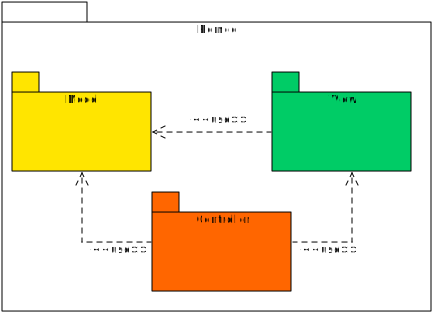
\includegraphics[scale=0.65] {../Specifica_Tecnica/Content/Immagini/Romeo.png}
			\caption{Componente Romeo}
			\label{romeoj}
\end{figure}

\section{Specifica componenti Romeo::Model}
\label{specificaModel}

\begin{figure} [!h]
\centering
	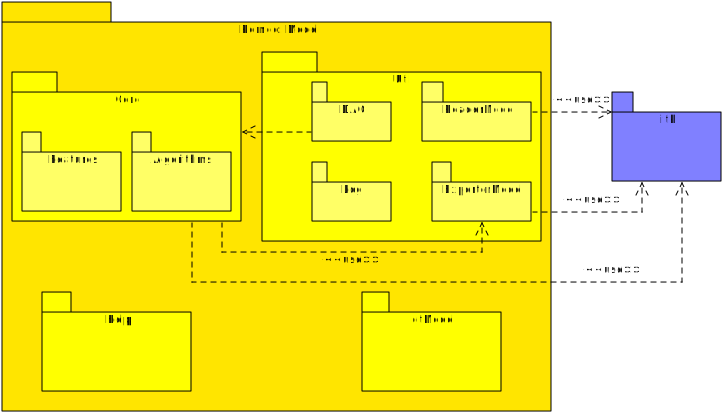
\includegraphics[scale=0.65] {../Specifica_Tecnica/Content/Immagini/Romeo__Model.png}
			\caption{Componente Romeo::Model}
			\label{comp_romeo_model}
\end{figure}

Package\g{} per il componente Model dell'architettura MVC.

\pagebreak
\subsection{Specifica componenti Model::Core}
\label{specifica_model_core}
\begin{figure}[!h]
\centering
			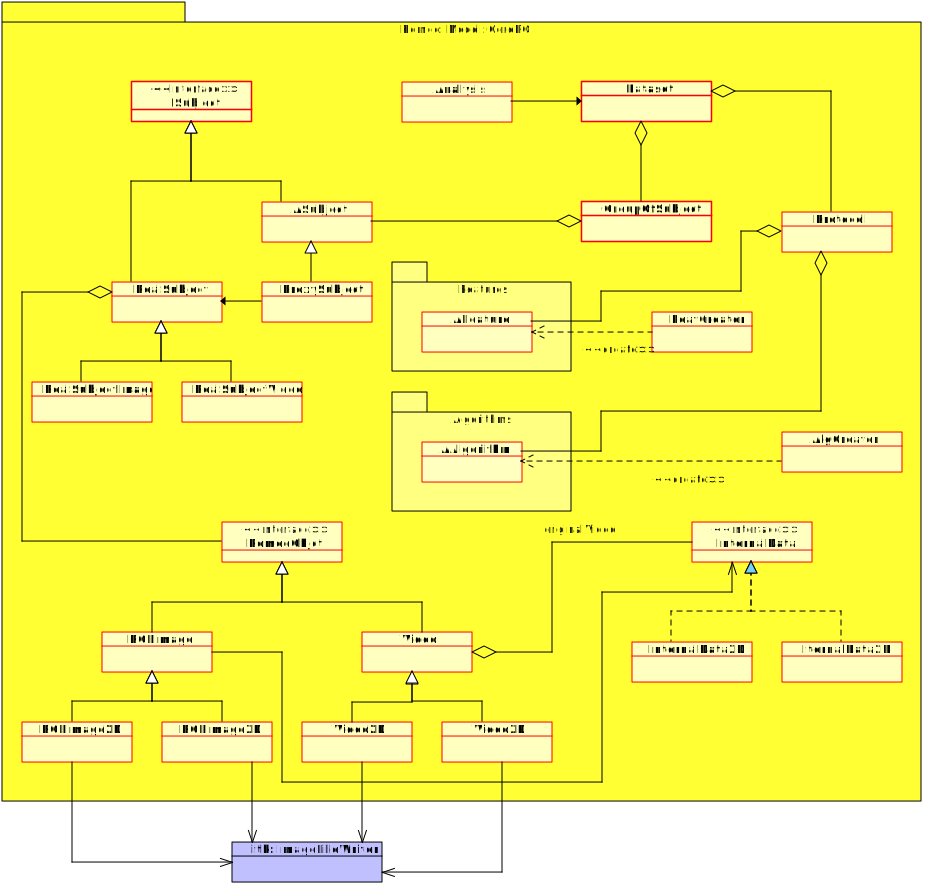
\includegraphics[scale=0.55]{../Specifica_Tecnica/Content/Immagini/Romeo__Model__Core.png}
			\caption{Diagramma package \textsl{Romeo::Model::Core}}
			\label{romeo_model_core}
\end{figure}
Package\g{} per il componente core.
% % % % % % % % % % % % % % % % % % % % % % % % % % % % % % % % % % %
% % ALGCREATOR % % % % % % % % % % % % % % % % % % % % % % % % % % % %
% % % % % % % % % % % % % % % % % % % % % % % % % % % % % % % % % % %

\subsubsection{AlgCreator (class)}
\label{algcreator}
	\begin{figure}[!h]
	\centering
				\includegraphics[scale=0.8]{./Content/Immagini/modelCore/AlgCreator.png}
				\caption{Diagramma classe \textsl{AlgCreator}}
				\label{algCreator_img}
	\end{figure}

	\paragraph{Descrizione\\}
	classe Factory avente la responsabilità di creare un oggetto di tipo \textsl{Romeo::Model::Core::Algorithms::AAlgorithm}, che rappresenta un' instanza dell' algoritmo da creare.
    \\Rappresenta il componente Factory del design pattern\g{} Factory.

	\paragraph{Utilizzo\\}
	viene utilizzata in seguito alla ricezione di un signal\g{} da parte dei controller che necessitano di utilizzare un oggetto di tipo \textsl{Romeo::Model::Core::Algorithms::AAlgorithm}.
	\\A seconda dei parametri e nome dell’ algoritmo di Cluster\g{} passati, crea un oggetto rispetto ad un altro.

	\paragraph{\textcolor{black}{Attributi\\}}
		\begin{itemize}
			\item \color{teal}\verb!- static algCreator: AlgCreator *!
			\color{black}
			\subparagraph{Descrizione:} puntatore all'unica istanza della classe \textsl{AlgCreator} che verrà creata in modo \textit{lazy} quando verrà richiesta la creazione dell'oggetto.
		\end{itemize}
		
\paragraph{\color{black}{Metodi}}
	\begin{itemize}
		%costruttore
		\item \color{blue}\verb! - AlgCreator()!
		\color{black}
		\subparagraph{Descrizione:} costruttore privato, come previsto dal design pattern\g{} Singleton.
		
		%getAlgCreator
		\item \color{blue}\verb! + static getAlgCreator : AlgCreator *!
		\color{black}
		\subparagraph{Descrizione:} metodo statico che  ritorna il puntatore all'unica istanza della classe \textsl{AlgCreator}. Nel caso in cui l'istanza non esista ancora, essa verrà creata e successivamente ritornata.
		\subparagraph{Note}
			\begin{itemize}
				\item Il metodo deve essere marcato come statico.
			\end{itemize}
			
		%buildAlgorithm
		\item \color{blue}\verb! + buildAlgorithm(name : const QString&, parameters : const QStringList& ,!
					\verb!algId : int) : AAlgorithm*!
		\color{black}
		\subparagraph{Descrizione:}Metodo che ha il compito di costruire l'algoritmo specificato, con i relativi parametri.\\
		Per esempio se il parametro \textit{name} è uguale a \lq\lq{}KMeans\rq\rq{} allora verrà creato un oggetto \textit{KMeansAlgorithm} con i dati passati nei parametri.
		\subparagraph{Argomenti}
			\begin{itemize}
				\item \color{RoyalPurple}\verb!name : const QString&!\\
				\color{black}Stringa che rappresenta il nome dell'algoritmo di clustering\g{} che si vuole creare;
				
				\item \color{RoyalPurple}\verb!parameters : const QStringList&!\\
				\color{black}Lista di stringhe che rappresenta i parametri da passare all'algoritmo di cluster\g{} che si vuole creare;
				
				\item \color{RoyalPurple}\verb!algId : int!\\
				\color{black}Rappresenta l'id da associare all'algorimo che si vuole creare. Nel caso non venga specificato assumerà il valore di default di \lq\lq{}-1\rq\rq{} che indica che l'algorimo non è già presente nel database.
			\end{itemize}
		\subparagraph{Note}
			\begin{itemize}
				\item Il metodo deve essere marcato come costante.
			\end{itemize}
	
	%getAllAlgorithms
	\item \color{blue}\verb! + getAllAlgorithms() : QVector<AAlgorithm *>!
	\color{black}
	\subparagraph{Descrizione:} metodo che ritorna tutte le possibili istanze di algoritmi di cluster\g{}.
	\subparagraph{Note}
		\begin{itemize}
			\item Il metodo deve essere marcato come costante.
		\end{itemize}
		
	\end{itemize}
	
\pagebreak
% % % % % % % % % % % % % % % % % % % % % % % % % % % %
% % ANALYSIS % % % % % % % % % % % % % % % % % % % % %
% % % % % % % % % % % % % % % % % % % % % % % % % % % % %
%\pagebreak
\color{black}
\subsubsection{Analysis (class)}
	\label{analysis}
	\begin{figure}[!h]
	\centering
				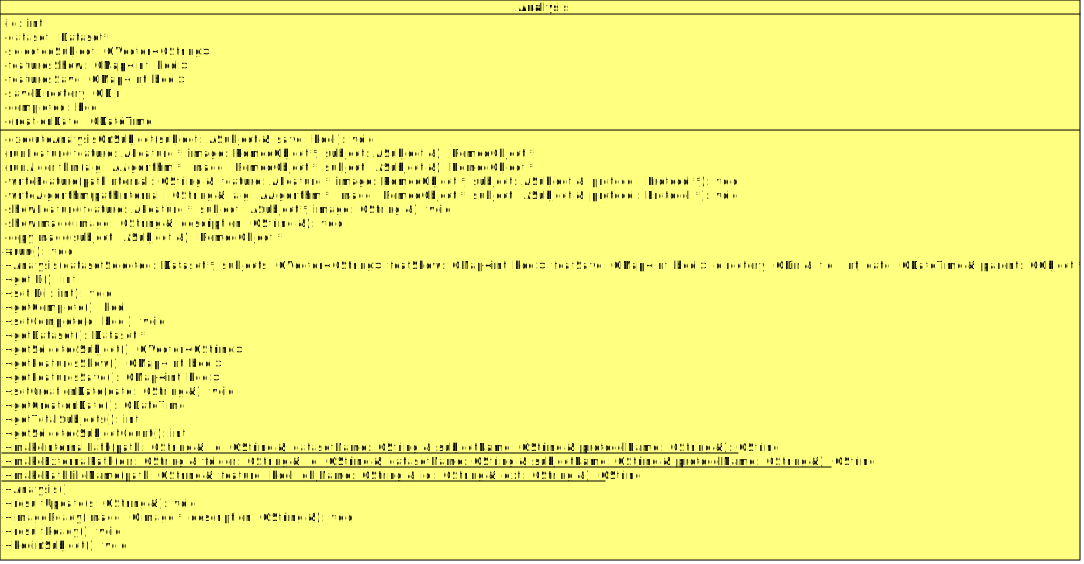
\includegraphics[scale=0.5]{./Content/Immagini/modelCore/Analysis.png}
				\caption{Diagramma classe \textsl{Analysis}}
				\label{analysis_img}
	\end{figure}

\paragraph{Descrizione \\}
classe che rappresenta un' analisi con le relative proprietà: \emph{Subject\g{} da analizzare, Directory dei risultati, Feature\g{} di cui salvare i risultati, Feature\g{} di cui visualizzare i risultati e Data di creazione}.
\\Rappresenta un Thread.

\paragraph{Utilizzo \\}
viene utilizzata dalla classe \textsl{AnalysisController}, alla ricezione di un signal\g{} per l'avvio di una nuova analisi.

\paragraph{Eredita da:}
	\begin{itemize}
		\item Qt::QThread.
	\end{itemize}
\paragraph{Attributi \\}
	\begin{itemize}
		\item \color{teal}\verb! - id : int!
		\color{black}
		\subparagraph{Descrizione:} rappresenta l'id associato all'analsi.
		
		\item \color{teal}\verb! - dataset!
		\color{black}
		\subparagraph{Descrizione:} puntatore all'oggetto \textsl{Dataset} associato all'analisi.
		
		\item \color{teal}\verb! - selectedSubject : QVector<QString>!
		\color{black}
		\subparagraph{Descrizione:} lista dei nomi dei Subject\g{} selezionati dall'utente su qui l'utente vuole eseguire l'analisi.
		
		\item \color{teal}\verb! - featuresShow : QMap<int, bool>!
		\color{black}
		\subparagraph{Descrizione:} mappa che rappresente le feature\g{} che l'utente vuole visualizzare nel dialogo.
		\\Ad ogni id delle feature è associato un \verb!bool! che indica se il risultato della feature\g{} deve essere visualizzata oppure no.
		
		\item \color{teal}\verb! - featuresSave : QMap<int, bool>!
		\color{black}
		\subparagraph{Descrizione:} mappa che rappresente le feature\g{} su cui l'utente vuole che siano esportati i risultati.
		\\Ad ogni id delle feature è associato un \verb!bool! che indica se il risultato della feature\g{} deve essere esportato oppure no.
		
		\item \color{teal}\verb! - saveDirectory : QDir!
		\color{black}
		\subparagraph{Descrizione:} cartella nel quale l'utente vuole che siano esportati i risultati.
		
		\item \color{teal}\verb! - completed : bool!
		\color{black}
		\subparagraph{Descrizione:} indica se l'analisi è terminata oppure no.
		
		\item \color{teal}\verb! - creationDate : QDateTime!
		\color{black}
		\subparagraph{Descrizione:} rappresenta la data in qui è stata avviata l'analisi.
			
	\end{itemize}

\color{black}
\paragraph{Metodi \\}
	\begin{itemize}
		%costruttore
		\item \color{blue}\verb! + Analysis(datasetSelected : Dataset *, subjects : QVector<QString>, !\\
								    \verb!featShow: const QMap<int, bool>, featSave : const QMap<int, bool>,!\\
							  		\verb! directory : const QDir&, tId : int, date : const QDateTime&, parent : QObject *);!\\
							  
		\color{black}
		\subparagraph{Descrizione:} costruttore della classe.
		
		\subparagraph{Argomenti:}
			\begin{itemize}
				\item \color{RoyalPurple}\verb!datasetSelected : Dataset *!\\
				\color{black}Puntatore al \textsl{Dataset} associato all'analisi;
				
				\item \color{RoyalPurple}\verb!subjects : QVector<QString>!\\
				\color{black}Lista dei nomi di Subject\g{} su qui eseguire l'analisi;
				
				\item \color{RoyalPurple}\verb!featShow: const QMap<int, bool>!\\
				\color{black}Mappa che associa ad un id di una feature\g{} un \verb!bool! che indica se la il risultato della feature\g{} va visualizzato nel dialogo oppure no;
				
				\item \color{RoyalPurple}\verb!featSave : const QMap<int, bool>!\\
				\color{black}Mappa che associa ad un id di uan feature\g{} un \verb!bool! che indica se il risultato della feature\g{} va esportato oppure no;
				
				\item \color{RoyalPurple}\verb!directory : const QDir&!\\
				\color{black}Directory nel quale salvare i risultati delle feature\g{} e degli algoritmi di clustering\g{};
				
				\item \color{RoyalPurple}\verb!tId : int!\\
				\color{black}Id associato all'analisi. Di default vale \lq\lq{}-1\rq\rq{};
				
				\item \color{RoyalPurple}\verb! date : const QDateTime&!\\
				\color{black}Data nel quale è stata creata l'analisi;
				
				\item \color{RoyalPurple}\verb!parent : QObject *!\\
				\color{black}Parente dell'oggetto Analysis.
			\end{itemize}
			
	\item \color{blue}\verb! - executeAnalysisOnSubject(subject : ASubject&, save : bool) : void!\\
	\color{black}\subparagraph{Descrizione:} metodo che esegue l'intera analisi sul \textsl{Subject} passato.
	\subparagraph{Argomenti}
		\begin{itemize}
			\item \color{RoyalPurple}\verb!subject : ASubject&!\\
			\color{black}Subject su qui eseguire l'analisi;
			
			\item \color{RoyalPurple}\verb!save : bool!\\
			\color{black}Booleano che indica se i risultati delle feature\g{} e degli algoritmi di clustering\g{} devono essere salvati o meno.
		\end{itemize}
	
	\item \color{blue}\verb! - runFeature(feature : AFeature *, image : RomeoObject *, !\\
	                            \verb!subject : ASubject &) : RomeoObject *!\\
	\color{black}\subparagraph{Descrizione:} metodo che esegue una feature\g{} sul formato interno dell'immagine passato come parametro.
	\\Ritorna un \textsl{RomeoObject *} rappresentante il formato interno dell'immagine di output.
	\subparagraph{Argomenti}
		\begin{itemize}
			\item \color{RoyalPurple}\verb!feature : AFeature *!\\
			\color{black}Feature da eseguire;
			
			\item \color{RoyalPurple}\verb!image : RomeoObject *!\\
			\color{black}Formato interno su cui eseguire la feature\g{};
			
			\item \color{RoyalPurple}\verb!subject : ASubject &!\\
			\color{black}Rappresenta il \textsl{Subject} su cui eseguire l'analisi.
		\end{itemize}
		
	\item \color{blue}\verb!- runAlgorithm(alg : AAlgorithm *, image : RomeoObject *, !\\
	                            \verb!subject : ASubject &) : RomeoObject *!\\
	\color{black}\subparagraph{Descrizione:} metodo che esegue un algoritmo\g{} sul formato interno dell'immagine passato come parametro.
	\\Ritorna un \textsl{RomeoObject *} rappresentante il formato interno dell'immagine di output.
	\subparagraph{Argomenti}
		\begin{itemize}
			\item \color{RoyalPurple}\verb!alg : AAlgorithm *!\\
					\color{black}Algoritmo da eseguire;
					
			\item \color{RoyalPurple}\verb!image : RomeoObject *!\\
			\color{black}Formato interno su cui eseguire la feature\g{};
		
			\item \color{RoyalPurple}\verb!subject : ASubject &!\\
			\color{black}Rappresenta il \textsl{Subject} su cui eseguire l'analisi.
		\end{itemize}
		
	\item \color{blue}\verb! - writeFeature(pathInternal : const QString&, !\\
								\verb!feature : AFeature*, image : RomeoObject *,subject : ASubject &,!\\
								\verb!protocol : Protocol *) : void!\\
			\color{black}\subparagraph{Descrizione:} metodo che esporta il risultato della feature\g{} nel filesystem.
			\subparagraph{Argomenti}
				\begin{itemize}
					\item \color{RoyalPurple}\verb!pathInternal : const QString&!\\
					\color{black}Path nel quale salvare il risultato della feature\g{};
					
					\item \color{RoyalPurple}\verb!feature : AFeature*!\\
					\color{black}Rappresenta la feature\g{} che è appena stata eseguita;
					
					\item \color{RoyalPurple}\verb!image : RomeoObject *!\\
					\color{black}Rappresenta il formato interno dell'imamgine che va esportata;
					
					\item \color{RoyalPurple}\verb!subject : ASubject &!\\
					\color{black}Rappresenta il Subject\g{} sul quale è stata eseguita la feature\g{};
					
					\item \color{RoyalPurple}\verb!protocol : Protocol *!\\
					\color{black}Rappresenta il Protocol\g{} al quale appartiene la Feature\g{} appena eseguita.
				\end{itemize}
				
		
	\item \color{blue}\verb! - writeAlgorithm(pathInternal : const QString&,!\\
	 						    \verb! alg : AAlgorithm*, image : RomeoObject *,!\\
									\verb! subject : ASubject &, protocol : Protocol *) : void!\\
				\color{black}\subparagraph{Descrizione:} metodo che esporta il risultato dell'algoritmo di clustering\g{} nel filesystem.
				\subparagraph{Argomenti}
					\begin{itemize}
						\item \color{RoyalPurple}\verb!pathInternal : const QString&!\\
						\color{black}Path nel quale salvare il risultato dell'algoritmo\g{};
						
						\item \color{RoyalPurple}\verb!alg : AAlgorithm*!\\
						\color{black}Rappresenta l'algoritmo di clustering\g{} che è appena stato eseguito;
						
						\item \color{RoyalPurple}\verb!image : RomeoObject *!\\
						\color{black}Rappresenta il formato interno dell'imamgine che va esportata;
						
						\item \color{RoyalPurple}\verb!subject : ASubject &!\\
						\color{black}Rappresenta il Subject\g{} sul quale è stato eseguito l'algorimo di clustering\g{};
						
						\item \color{RoyalPurple}\verb!protocol : Protocol *!\\
						\color{black}Rappresenta il Protocol\g{} al quale appartiene l'algoritmo di clustering\g{} appena eseguito.
					\end{itemize}
	
	\item \color{blue}\verb! - showFeature(feature : AFeature *, subject : ASubject *,!\\
						       \verb! image : const QString &) : void!\\
			 \color{black}\subparagraph{Descrizione:} metodo che si occupa di creare un oggetto \verb!QImage! sul risultato di una feature\g{}.
			 \subparagraph{Argomenti}
			 	\begin{itemize}
				 	\item \color{RoyalPurple}\verb!feature : AFeature *!\\
				 	\color{black}Rappresenta la feature\g{} che è stata eseguita;
				 	
				 	\item \color{RoyalPurple}\verb!subject : ASubject *!\\
				 	\color{black}Rappresenta il Subject\g{} su cui è stata eseguita la feature\g{};
				 	
				 	\item \color{RoyalPurple}\verb!image : const QString &!\\
				 	\color{black}Percorso nel quale è presente il risultato della feature\g{} appena eseguita.
			 	\end{itemize}
	
	\item \color{blue}\verb! - showImage(image : const QString &, type : const QString &,!\\
								\verb! description : const QString &) : void!\\
	\color{black}\subparagraph{Descrizione:}  metodo che emette il signal\g{} \verb!imageReady! quando un algoritmo di clustering\g{} o una feature\g{} è terminata.
	\subparagraph{Argomenti}
		\begin{itemize}
			\item \color{RoyalPurple}\verb!image : const QString &!\\
			\color{black}Rappreenta il percorso nel quale si trova l'immagine risultato;
			
			\item \color{RoyalPurple}\verb!type : const QString &!\\
			\color{black}Rappresenta il tipo di immagine;
			
			\item \color{RoyalPurple}\verb!description : const QString &)!\\
			\color{black}Rappresenta la descrizione dell'immagine.
		\end{itemize}
		
	\item \color{blue}\verb! + run() : void!\\
	\color{black}\subparagraph{Descrizione:} avvia il thread.
	\subparagraph{Note}
		\begin{itemize}
			\item Il metodo deve essere marcato come virtuale.
		\end{itemize}
	
	\item \color{blue}\verb! + getID() :int!\\
	\color{black}\subparagraph{Descrizione:} metodo che ritorna l'id associato all'istanza.
	\subparagraph{Note}
		\begin{itemize}
			\item Il metodo deve essere marcato costante.
		\end{itemize}
		
	\item \color{blue}\verb! + setID(i : int) : void!\\
	\color{black}\subparagraph{Descrizione:} cambia l'id associato all'oggetto \textsl{Analysis}.
	\subparagraph{Argomenti}
		\begin{itemize}
			\item \color{RoyalPurple}\verb!i : int!\\
			\color{black}Il nuovo id da associare.
		\end{itemize}
		
	\item \color{blue}\verb! + getComplete() : bool!\\
	\color{black}\subparagraph{Descrizione:} ritorna un \verb!bool! che indica se l'analisi è stata terminata o meno.
	\subparagraph{Note}
		\begin{itemize}
			\item Il metodo deve essere marcato come costante.
		\end{itemize}
		
	\item \color{blue}\verb! + setComplete(c : bool) : void!\\
	\color{black}\subparagraph{Descrizione:} metodo che cambia lo stato di completamento dell'analisi.
	\subparagraph{Argomenti}
		\begin{itemize}
			\item \color{RoyalPurple}\verb!c : bool!\\
			Rappresenta il nuovo stato di completamento dell'analsi.
		\end{itemize}
		
	\item \color{blue}\verb!+ getDataset() : Dataset*!\\
	\color{black}\subparagraph{Descrizione:} metodo che ritorna l'oggetto \textsl{Dataset} associato all'analisi.
	\subparagraph{Note}
		\begin{itemize}
			\item Il metodo deve essere marcato come costante.
		\end{itemize}
		
	\item \color{blue}\verb! + getSelectedSubject() : QVector<QString>!\\
	\color{black}\subparagraph{Descrizione:} metodo che ritorna la lista dei Subject\g{} su cui eseguire l'analisi.
	\subparagraph{Note}
		\begin{itemize}
			\item Il metodo deve essre marcato come costante.
		\end{itemize}
		
	\item \color{blue}\verb! + getFeaturesShow() : QMap<int, bool>!\\
	\color{black}\subparagraph{Descrizione:} metodo che ritorna una \verb! QMap! che associa all'id di una feature un \verb!bool! che indica se il risultato della feature\g{} va visualizzati nel dialogo oppure no.
	\subparagraph{Note}
		\begin{itemize}
			\item Il metodo deve essere marcato come costante.
		\end{itemize}
		
	\item \color{blue}\verb! +  getFeaturesSave() :QMap<int, bool>!\\
	\color{black}\subparagraph{Descrizione:} metodo che ritorna una \verb! QMap! che associa all'id di una feature un \verb!bool! che indica se il risultato della feature\g{} va esportato oppure no.
		\subparagraph{Note}
			\begin{itemize}
				\item Il metodo deve essere marcato come costante.
			\end{itemize}
			
	\item \color{blue}\verb! + setCreationDate(date : const QString &) : void!\\
	\color{black}\subparagraph{Descrizione:} metodo che cambia la data di creazione di un oggetto \textsl{Analysis}.
	\subparagraph{Argomenti}
		\begin{itemize}
			\item \color{RoyalPurple}\verb!date : const QString &!\\
			\color{black}Nuova data di creazione.
		\end{itemize}
		
	\item \color{blue}\verb! + getCreationDate() : QDateTime!\\
	\color{black}\subparagraph{Descrizione:} metodo che ritorna la data di creazione di un oggetto \textsl{Analysis}.
	\subparagraph{Note}
	\begin{itemize}
		\item Il metodo va marcato come costante.
	\end{itemize}
	
	\item \color{blue}\verb! + getTotalSubjects() :int!\\
	\color{black}\subparagraph{Descrizione:} metodo che ritorna il numero di Subject\g{} presenti nel Gruppo di Subject associati al Dataset\g{} dell'analisi.
	\subparagraph{Note}
		\begin{itemize}
			\item Il metodo deve essere marcato costante.
		\end{itemize}
		
	\item \color{blue}\verb! + getSelectedSubjectCount() : int!\\
	\color{black}\subparagraph{Descrizione:} metodo che ritorna il numero di Subject\g{} su cui eseguire l'analisi.
	\subparagraph{Note}
		\begin{itemize}
			\item Il metodo deve essere marcato costante.
		\end{itemize}
		
	\item \color{blue}\verb! + resultUpdate(s : const QString &) : void (signal)!\\    
	\color{black}\subparagraph{Descrizione:} signal\g{} emesso quando va aggiornata la descrizione dell'oggetto \textsl{AnalysisDialog}.
	\subparagraph{Argomenti}
		\begin{itemize}
			\item \color{RoyalPurple}\verb!s : const QString &!\\
			\color{black}Nuovo testo da visualizzare nel dialogo.
		\end{itemize}   
		
	\item \color{blue}\verb! + imageReady(image : QImage *, description : const QString &) : void (signal)!\\
	\color{black}\subparagraph{Descrizione:} signal\g{} emesso quando una nuova immagine è disponibile.
	\subparagraph{Argomenti}
		\begin{itemize}
			\item \color{RoyalPurple}\verb!image : QImage *!\\
			\color{black}Nuova immagine disponibile;
			
			\item \color{RoyalPurple}\verb!description : const QString &!\\
			\color{black}Descrizione associata all'immagine.
		\end{itemize}
		
	\item \color{blue}\verb! + resultReady() : void (signal)!\\
	\color{black}\subparagraph{Descrizione:} signal\g{} emesso quando l'esecuzione dell'analisi è terminata.
	
	\item \color{blue}\verb! +beginSubject() : void (signal)!\\
	\color{black}\subparagraph{Descrizione:} signal\g{} emesso quando l'analisi viene effettuata su un nuovo Subject\g{}.

	\end{itemize}
 


\pagebreak
% % % % % % % % % % % % % % % % % % % % % % % % % % % % % 
% % ISubject & % % % % % % % % % % % % % % % % % % % % %
% % % % % % % % % % % % % % % % % % % % % % % % % % % % %
\color{black}
\subsubsection{ISubject (interface)}
\label{iSubject}
\begin{figure}[!h]
\centering
			\centering
			 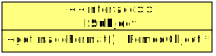
\includegraphics[scale=1.00]{./Content/Immagini/modelCore/ISubject.png}
			 \caption{Diagramma classe \textsl{ISubject}}
			\label{iSubject_img}
\end{figure}

\paragraph{Descrizione \\}
	Definisce l’interfaccia comune per le classi \textsl{ASubject} e \textsl{RealSubjec}, fornisce un metodo per ottenere il formato interno per l’immagine del Subject\g{}.
	\\Rappresenta il componente Subject del design pattern\g{} Proxy.

\paragraph{Utilizzo \\}
Viene utilizzata quando le componenti di Romeo\g{} necessitano di riferirsi a un Subject\g{} per ottenere il formato interno ad esso associato. 

\paragraph{\color{black}Metodi}
\begin{itemize}
			\item \color{blue} \verb!+ getImageFormat() : RomeoObject *!
			\color{black}
			\subparagraph{Descrizione:} contratto che restituisce un puntatore al formato interno dell'immagine di un Subject\g{}
			\subparagraph{Note}
			\begin{itemize}
				\item Il metodo deve essere marcato come virtuale.
			\end{itemize}
\end{itemize}
\pagebreak
% % % % % % % % % % % % % % % % % % % % % % % % % % % % % 
% % ASubject & % % % % % % % % % % % % % % % % % % % % %
% % % % % % % % % % % % % % % % % % % % % % % % % % % % %
\color{black}
\subsubsection{ASubject (abstract)}
\label{aSubject}
\begin{figure}[!h]
\centering
			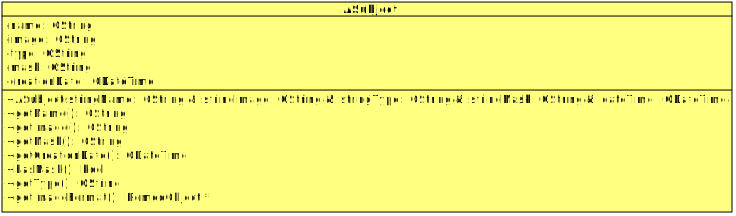
\includegraphics[scale=0.80]{./Content/Immagini/modelCore/ASubject}
			\caption{Diagramma classe \textsl{ASubject}}
			\label{aSubject_img}
\end{figure}

\paragraph{Descrizione \\}
Classe astratta che rappresenta un generico Subject\g{} con le relative proprietà \emph{Nome, Tipo del Subject\g{}, Immagine, Maschera e Data di creazione}.

\paragraph{Utilizzo \\}
 Viene utilizzata in seguito alla ricezione di un signal\g{} da parte dei controller che necessitano di riferirsi ad uno o più oggetti di tipo \textsl{ASubject}.
 \\Inoltre viene utilizzata dalle classi DAO e dalla classe \textsl{GroupOfSubject}.
 
\paragraph{Eredita da:}
\begin{itemize}
	\item Romeo::Model::Core::ISubject: non implementa ancora i contratti di questa classe.
\end{itemize}

\paragraph{Attributi \\}
	\begin{itemize}
			\item \color{teal} \verb!- name : QString!
					\color{black}
					\subparagraph{Descrizione:} nome del Subject\g{}.
					\item \color{teal} \verb!- image : QString!
					\color{black}
					\subparagraph{Descrizione:} stringa rappresentante il percorso assoluto dell'immagine del Subject\g{}.
					\item \color{teal} \verb!- type : QString!
					\color{black}
					\subparagraph{Descrizione:} stringa rappresentante il tipo di un Subject\g{} (2D, 2D-t, 3D, 3D-t).
					\item \color{teal} \verb!- mask : QString!
					\color{black}
					\subparagraph{Descrizione} stringa rappresentante il percorso della maschera del Subject\g{}.
					\item \color{teal} \verb!- creationDate : QDateTime!
					\color{black}
					\subparagraph{Descrizione:} data di creazione del Subject\g{}
	\end{itemize}
	
\paragraph{\color{black}Metodi \\}
\begin{itemize}

			%Costruttore
			\item \color{blue} \verb!+ ASubject(stringName : const QString &, stringImage : const QString &,!
			\verb!stringType : const QString &, stringMask : const QString &, dateTime : const QDateTime &)!
			\color{black}
			\subparagraph{Descrizione:} costruttore della classe.
			\color{black}
			\subparagraph{Argomenti}
				\begin{itemize}
					\item \color{RoyalPurple} \verb!stringName : const QString &!\\				
								\color{black} Nome del Subject\g{}.
					\item \color{RoyalPurple} \verb!stringImage : const QString &!\\				
								\color{black} Percorso dell'immagine del Subject\g{};
					\item \color{RoyalPurple} \verb!stringType : const QString &!\\				
								\color{black} Stringa che rappresenta il tipo del Subject\g{} (2D, 2D-t, 3D, 3D-t).
					\item \color{RoyalPurple} \verb!stringMask : const QString &!\\				
							  \color{black} Stringa rappresentante il percorso della maschera del Subject\g{}.
					\item \color{RoyalPurple} \verb!dateTime : const QDateTime &!\\				
								\color{black} Data di creazione del Subject\g{}.
				\end{itemize}
			
			%getName	
			\item \color{blue} \verb!+ getName() : QString! 
			\color{black}
			\subparagraph{Descrizione:} metodo che ritorna una stringa, contenente il nome del Subject\g{}.
			\subparagraph{Note}
			\begin{itemize}
				\item Il metodo deve essere marcato costante.
			\end{itemize}
			
			%getImage
			\item \color{blue} \verb!+ getImage() : QString! 
			\color{black}
			\subparagraph{Descrizione:} metodo che ritorna una stringa, contenete il percorso assoluto dell'immagine associata al Subject\g{}.
			\subparagraph{Note}
			\begin{itemize}
				\item Il metodo deve essere marcato costante.
			\end{itemize}
			
			%getMask
			\item \color{blue} \verb!+ getMask() : QString! 
			\color{black}
			\subparagraph{Descrizione:} metodo che ritorna una stringa, contente il percorso assoluto della (eventuale) maschera associata al Subject\g{}.
			\subparagraph{Note}
			\begin{itemize}
				\item Il metodo deve essere marcato costante.
			\end{itemize}
			
			%getCreationDate
			\item \color{blue} \verb!+ getCreationDate() : QDateTime!
			\color{black}
			\subparagraph{Descrizione:} metodo che ritorna la data di creazione del Subject\g{}.
			\subparagraph{Note}
			\begin{itemize}
				\item Il metodo deve essere marcato costante.
			\end{itemize}
			
			%hasMask
			\item \color{blue} \verb!+ hasMask() : bool!
			\color{black}
			\subparagraph{Descrizione:} metodo che controlla se il Subject\g{} contiene una maschera\g{} oppure no.
			\\Ritorna \verb!true! se il Subject\g{} possiede una maschera, \verb!false! viceversa.
			\subparagraph{Note}
			\begin{itemize}
				\item Il metodo deve essere marcato costante.
			\end{itemize}
			
			%getType
			\item \color{blue} \verb!+ getType() : QString!
			\color{black}
			\subparagraph{Descrizione} Metodo che ritorna una stringa, contente il tipo del Subject\g{} (2D, 2-t, 3D, 3D-t).
			\subparagraph{Note}
			\begin{itemize}
				\item Il metodo deve essere marcato const.
			\end{itemize}
		\end{itemize}


% % % % % % % % % % % % % % % % % % % % % % % % % % % % % 
% % ProxySubject & % % % % % % % % % % % % % % % % % % % % %
% % % % % % % % % % % % % % % % % % % % % % % % % % % % %
\pagebreak
\color{black}
\subsubsection{ProxySubject (class)}
\label{proxySubject}
\begin{figure}[!h]
\centering
			\includegraphics[width=1\linewidth]{./Content/Immagini/modelCore/ProxySubject.png}
			\caption{Diagramma classe \textsl{ProxySubject}}
			\label{proxySubject_img}
\end{figure}

\paragraph{Descrizione \\}
Classe che gestisce l’accesso ad un \textsl{RealSubject}, mantiene un riferimento che consente al proxy di accedere all’oggetto rappresentato \textsl{RealSubject}.
\\Fornisce la stessa interfaaccia della classe \textsl{ASubject}, consentendo di utilizzare un oggetto \textsl{ProxySubject} quando è richiesto un oggetto \textsl{ASubject}.
\\Rappresenta il componente Proxy del design pattern\g{} Proxy.

\paragraph{Utilizzo \\}
Viene utilizzando quando è necessario creare un Subject\g{} all'interno di Romeo\g{}.

\paragraph{Eredita da:}
\begin{itemize}
	\item Romeo::Model::Core::ISubject: implementa i contratti di questa classe.
\end{itemize}

\paragraph{Attributi \\}
	\begin{itemize}
		\item \color{teal}\verb! - realSubject : RealSubject *!
		\color{black}
		\subparagraph{Descrizione:} puntatore ad un oggetto di tipo \textsl{RealSubject} che il Proxy sta rappresentando.
	\end{itemize}

\color{black}
\paragraph{Metodi \\}
	\begin{itemize}
		%costruttore
		\item  \color{blue}\verb! + ProxySubject(subjectName : const QString&, subjectImage : const QString&, !\\
			\verb!maskName : const QString&, dateTime : const QDateTime&)!
			\color{black}
			\subparagraph{Descrizione:} costruttore della classe. Richiama il costruttore della superclasse.
			\subparagraph{Argomenti}
				\begin{itemize}
					\item \color{RoyalPurple}\verb!subjectName : const QString&!\\
					\color{black}Nome del Subject\g{}. Viene passato al costruttore della superclasse;
					
					\item \color{RoyalPurple}\verb!subjectImage : const QString&!\\
					\color{black}Immagine del Subject\g{}. Viene passato al costruttore della superclasse;
					
					\item \color{RoyalPurple}\verb!maskName : const QString&!\\
					\color{black}Maschera\g{} del \subject{}. Viene passato al costruttore della superclasse;
					
					\item \color{RoyalPurple}\verb!dateTime : QDateTime &!\\
					\color{black}Data di creazione del \subject{}. Viene passato al costruttore della superclasse.
				\end{itemize}
		
		%getRealSubject
		\item \color{blue}\verb! # getRealSubject() : RealSubject *!
		\color{black}
		\subparagraph{Descrizione:} restituisce il puntatore al \textsl{RealSubject} rappresentato. Nel caso non esista viene creato e successivmente ritornato.
		
		%getImageFormat
		\item \color{blue}\verb! + getImageFormat() : RomeoObject *!
		\color{black}
		\subparagraph{Descrizione:} Implementa il contratto fornito dalla superclasse. Si limita a chiamare il metodo \verb!getImageFormat()! sull'oggetto \textsl{RealSubject}.
		
		\subparagraph{Note}
			\begin{itemize}
				\item Il metodo deve essere marcato virtuale.
			\end{itemize}
			
	\end{itemize}


\pagebreak
% % % % % % % % % % % % % % % % % % % % % % % % % % % % % 
% % RealSubject & % % % % % % % % % % % % % % % % % % % % %
% % % % % % % % % % % % % % % % % % % % % % % % % % % % %
\color{black}
\subsubsection{RealSubject (abstract)}
\label{RealSubject}
\begin{figure}[!h]
\centering
			\includegraphics[scale=1]{./Content/Immagini/modelCore/RealSubject.png}
			\caption{Diagramma classe \textsl{RealSubject}}
			\label{realSubject_img}
\end{figure}

\paragraph{Descrizione \\}
classe astratta che caratterizza l’oggetto rappresentato dal \textsl{ProxySubject}, rappresenta un oggetto reale utilizzato dalla classe \textsl{ProxySubject}.
\\Contiene la proprietà \emph{imageFormat}.
\\Le sottoclassi rappresentano i componenti RealSubject del design pattern\g{} Proxy.

\paragraph{Utilizzo \\}
 viene utilizzato dalla classe \textsl{ProxySubject}, la quale contiene un riferimento al \textsl{RealSubject} che sta gestendo.
 
\paragraph{Eredita da:}
\begin{itemize}
	\item Romeo::Model::Core::ISubject: implementa i contratti di questa classe.
\end{itemize}

\paragraph{Attributi}
	\begin{itemize}
	   %imageFormat
		\item \color{teal}\verb! # imageFormat : RomeoObject *!
		\color{black}
		\subparagraph{Descrizione:} puntatore al formato interno utilizzato per rappresentare l'immagine associata al Subject\g{}.
	\end{itemize}

\paragraph{\color{black}Metodi}
	\begin{itemize}
		%costruttore
		\item \color{blue}\verb! # RealSubject()!
		\color{black}
		\subparagraph{Descrizione:} costruttore della classe. Il costruttore è stato reso protetto in quanto la classe è ancora astratta.
	\end{itemize}

\pagebreak
% % % % % % % % % % % % % % % % % % % % % % % % % % % % % 
% % RealSubjectImage & % % % % % % % % % % % % % % % % % % % % %
% % % % % % % % % % % % % % % % % % % % % % % % % % % % %
\color{black}
\subsubsection{RealSubjectImage (class)}
\label{RealSubject2D}
\begin{figure}[!h]
\centering
			\includegraphics[scale=1]{./Content/Immagini/modelCore/RealSubjectImage.png}
			\caption{Diagramma classe \textsl{RealSubjectImage}}
			\label{realSubject2d_img}
\end{figure}

\paragraph{Descrizione \\}
Classe concreta che rappresenta un Subject\g{} nel formato bidimensionale (2D, 3D).

\paragraph{Utilizzo \\}
Viene utilizzata dalla classe \textsl{ProxySubject} per ottenere l'oggetto di tipo \textsl{RomeoObject} che rappresenta l'immagine, quando il \textsl{ProxySubject} sta rappresentando un Subject\g{} 2D o 3D.

\paragraph{Eredita da:}
\begin{itemize}
	\item Romeo::Model::Core::RealSubject.
\end{itemize}

\paragraph{Metodi \\}
	\begin{itemize}
		\item \color{blue}\verb! + RealSubjectImage(image : const QString &, mask : const QString &)!
		\color{black}
		\subparagraph{Descrizione:} costruttore della classe. Richiama il costruttore della supeclasse.
		\\Rappresenta il componente RealSubject del design pattern\g{} Proxy.
		
		\subparagraph{Argomenti}
			\begin{itemize}
				\item \color{RoyalPurple}\verb!image : const QString &!\\
				\color{black}Stringa che rappresenta il path nel quale è presente l'immagine del Subject\g{};
				
				\item \color{RoyalPurple}\verb!mask : const QString &)!\\
				\color{black}Stringa che rappresenta il path nel quale è presente la maschera del Subject\g{}.
				Nel caso in qui il Subject\g{} non abbia alcuna maschera l'argomento \verb!mask! assumerà il valore di default "".
			\end{itemize}
	\end{itemize}

\pagebreak
% % % % % % % % % % % % % % % % % % % % % % % % % % % % % 
% % RealSubjectVideo & % % % % % % % % % % % % % % % % % % % % %
% % % % % % % % % % % % % % % % % % % % % % % % % % % % %
\color{black}
\subsubsection{RealSubjectVideo (class)}
\label{RealSubject3D}
\begin{figure}[!h]
\centering
			\includegraphics[scale=1]{./Content/Immagini/modelCore/RealSubjectVideo.png}
			\caption{Diagramma classe \textsl{RealSubjectVideo}}
			\label{realSubject3d_img}
\end{figure}

\paragraph{Descrizione \\}
Classe concreta che rappresenta un Subject\g{} di tipo 2D-t o 3D-t.
\\Rappresenta il componente RealSubject del design pattern\g{} proxy.

\paragraph{Utilizzo \\}
Viene utilizzata dalla classe \textsl{ProxySubject} per ottenere l'oggetto di tipo \textsl{RomeoObject} che rappresenta l'immagine, quando il \textsl{ProxySubject} sta rappresentando un Subject\g{} 2D-t o 3D-t.
			

\paragraph{Eredita da:}
\begin{itemize}
	\item Romeo::Model::Core::RealSubject.
\end{itemize}

\paragraph{Metodi \\}
\begin{itemize}
		\item \color{blue}\verb! + RealSubjectVideo(image : const QString &, mask : const QString &)!
		\color{black}
		\subparagraph{Descrizione:} costruttore della classe. Richiama il costruttore della supeclasse.
		\\Rappresenta il componente RealSubject del design pattern\g{} Proxy.
		
		\subparagraph{Argomenti}
			\begin{itemize}
				\item \color{RoyalPurple}\verb!image : const QString &!\\
				\color{black}Stringa che rappresenta il path nel quale è presente l'immagine del Subject\g{};
				
				\item \color{RoyalPurple}\verb!mask : const QString &)!\\
				\color{black}Stringa che rappresenta il path nel quale è presente la maschera del Subject\g{}.
				Nel caso in qui il Subject\g{} non abbia alcuna maschera l'argomento \verb!mask! assumerà il valore di default "".
			\end{itemize}
	\end{itemize}

\pagebreak
% % % % % % % % % % % % % % % % % % % % % % % % % % % % % 
% % GroupOfSubject % % % % % % % % % % % % % % % % % % % % %
% % % % % % % % % % % % % % % % % % % % % % % % % % % % %
\color{black}
\subsubsection{GroupOfSubject (class)}
\label{groupOfSubject}
\begin{figure}[!h]
\centering
			\includegraphics[width=1.2\linewidth]{./Content/Immagini/modelCore/GroupOfSubject.png}
			\caption{Diagramma classe \textsl{GroupOfSubject}}
			\label{groupOfSubject_img}
\end{figure}

\paragraph{Descrizione \\}
Classe che rappresenta un gruppo di Subject\g{} con le relative propietà: \emph{Nome del gruppo, tipo del gruppo, data di creazione e la lista di Subject\g{} presenti nel gruppo}.

\paragraph{Utilizzo \\}
Viene utilizzata in seguito alla ricezione di un signal\g{} da parte dei controller che necessitano di riferirsi ad uno o più gruppi di Subject\g{}
\\Inoltre viene utilizzata dalla classe \textsl{Dataset}, che contiene un riferimento al GroupOfSubject\g{} associato e dalle classi DAO.

\paragraph{Attributi }
	\begin{itemize}
		\item \color{teal}\verb!- imageType : QString!
		\color{black}\subparagraph{Descrizione:} stringa rappresentante il tipo del gruppo.
		
		% name
		
		\item \color{teal}\verb!- name : QString !
		\color{black}\subparagraph{Descrizione:} nome del gruppo.
			
		% mask
		\item \color{teal}\verb!- subjects : QVector<ASubject*> !
			\color{black}\subparagraph{Descrizione:} vettore di puntatori ad \textsl{ASubject} contenente i \subject{} facenti parte del gruppo.

		% creationDate
		\item \color{teal}\verb!- creationDate : QDateTime !
			\color{black}\subparagraph{Descrizione:} data di creazione del gruppo.
	\end{itemize}
	
\paragraph{Metodi \\}
	\begin{itemize}
		\item \color{blue}\verb! + GroupOfSubject(nameGroup : const QString&, imageType : const QString&,!\\
									 \verb! subjectsV : QVector<ASubject*>  ,  dateTime : const QDateTime&)!\\
				\color{black}
					\subparagraph{Descrizione:} costruttore della classe \textsl{GroupOfSubjcect}.
					\subparagraph{Argomenti}
						\begin{itemize}
							\item \color{RoyalPurple}\verb!nameGroup : const QString&!\\
							\color{black}Nome del Gruppo di Subject\g{};
							
							\item \color{RoyalPurple}\verb!imageType : const QString&!\\
							\color{black}Tipo del Gruppo di Subject\g{ (2D, 2D-t, 3D, 3D-t)};
							
							\item \color{RoyalPurple}\verb!subjectsV : QVector<ASubject*>!\\
							\color{black}Subject\g{} presenti nel gruppo;
							
							\item \color{RoyalPurple}\verb!dateTime : const QDateTime&!\\
							\color{black}Data di creazione del Subject\g{}.
						\end{itemize}
						
		\item \color{blue}\verb! + getName() : QString !\\
		\color{black}
		\subparagraph{Descrizione:} ritorna una stringa contenente il nome del gruppo.
		\subparagraph{Note}
			\begin{itemize}
				\item Il metodo deve essere marcato come costante.
			\end{itemize}
			
		
		\item \color{blue}\verb! + getImageType() : QString !\\
		\color{black}
		\subparagraph{Descrizione:} ritorna una stringa contenente il percorso del gruppo.
		\subparagraph{Note}
			\begin{itemize}
				\item Deve essere marcato costante.
			\end{itemize}
			
		\item 	\color{blue}\verb! + getCreationDate() : QDateTime !\\
		\color{black}
		\subparagraph{Descrizione:} ritorna la data di craezione del gruppo di Subjcect.
		\subparagraph{Note}
			\begin{itemize}
				\item Deve essere marcato come costante.
			\end{itemize}
		
		\item \color{blue}\verb! + addSubject( subject : const ASubject& ) : void !\\
		\color{black}
		\subparagraph{Descrizione:} aggiunge un \subject{} al vettore dei \subject{} del gruppo.
		\subparagraph{Argomenti}
				\begin{itemize}
					\item \color{RoyalPurple}\verb!subject : const ASubject &! \\ 
					\color{black}\subject{} da inserire.
				\end{itemize}
		
		\item 	\color{blue}\verb! + containsSubject( subject : const ASubject& ) : boolean !\\
			\color{black} 
			\subparagraph{Descrizione:} ritorna un booleano per indicare se il gruppo contiene o meno un determinato \subject{}.
			\subparagraph{Argomenti}
				\begin{itemize}
					\item \color{RoyalPurple}\verb!subject : const ASubject &! \\
					\color{black} \subject{} da cercare.
				\end{itemize}
			
		\item 	\color{blue}\verb! + getSubjectWithName(name : const QString &) : ASubject * !
		\color{black}
		\subparagraph{Descrizione:} metodo  che ritorna un puntatore al \subject{} avente il nome richiesto.
		\subparagraph{Argomenti}
			\begin{itemize}
				\item \color{RoyalPurple}\verb!name : const QString &! \\ 
				\color{black}Nome del \subject{} da cercare.
			\end{itemize}	
		\subparagraph{Note}
			\begin{itemize}
				\item Il metodo deve essre marcato costante
			\end{itemize}
			
		% removeSubject
		\item \color{blue}\verb! + removeSubject( subject : const ASubject& ) : boolean !
		\color{black}
			\subparagraph{Descrizione:} rimuove un \subject{} dal vettore dei \subject{} del gruppo. Ritorna un booleano per indicare se l'operazione è andata a buon fine o meno.
			\subparagraph{Argomenti}
				\begin{itemize}
					\item \color{RoyalPurple}\verb!subject : const ASubject &! \\ 
					\color{black}\subject{} da rimuovere.
				\end{itemize}
			

		% getAllSubject
		\item \color{blue}\verb! + getAllSubject() : QVector<ASubject*> !\\
		\color{black}
		\subparagraph{Descrizione:} ritorna un vettore contenente i puntatori a tutti i \subject{} del gruppo.
		\subparagraph{Note}
			\begin{itemize}
				\item Il metodo deve essere marcato come costante.
			\end{itemize}
			
		%subjacetCount
		\item \color{blue}\verb! + subjectsCount() : int!\\
		\color{black}
		\subparagraph{Descrizione:} metodo che ritorna il number di subject nel gruppo.
		\subparagraph{Note}
			\begin{itemize}
				\item Il metodo deve essere marcato costante.
			\end{itemize}

	\end{itemize}
\pagebreak
% % % % % % % % % % % % % % % % % % % % % % % % % % % % % 
% % Protocol % % % % % % % % % % % % % % % % % % % % %
% % % % % % % % % % % % % % % % % % % % % % % % % % % % %
\color{black}
\subsubsection{Protocol (class)}
\label{Protocol}
\begin{figure}[!h]
\centering
			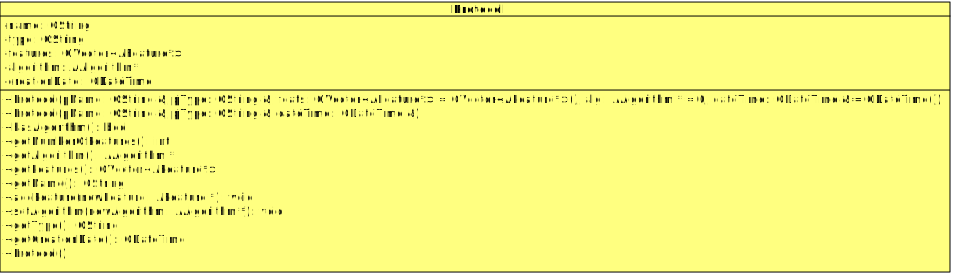
\includegraphics[scale=0.6]{./Content/Immagini/modelCore/Protocol.png}
			\caption{Diagramma classe \textsl{Protocol}}
			\label{Protocol_img}
\end{figure}

\paragraph{Descrizione \\}
Classe che rappresenta un Protocol\g{} con le relative propietà: \emph{Nome, Tipo, Data di creazione, Lista di feature\g{} e Algoritmo di cluster\g{}}.

\paragraph{Utilizzo \\}
viene utilizzata in seguito alla ricezione di un signal\g{} da parte dei controller che necessitano di riferirsi ad uno o più Protocol\g{}.
\\Inoltre viene utilizzata dalla classe \textsl{Dataset}, che contiene un riferimento ai Protocol\g{} associati, e dalle classi DAO.

\paragraph{Attributi}
	\begin{itemize}
	 	% name
		\item \color{teal}\verb!- name : QString !
		\color{black}\subparagraph{Descrizione:} nome del \protocol{}.
		
		%tpye
		\item \color{teal}\verb! -type : QString !
		\color{black}\subparagraph{Descrizione:} il tipo del Protocol\g{} (2D, 2D-t, 3D, 3D-t).
		
		% features
		\item \color{teal}\verb!- features : QVector<AFeature*> !
		\color{black} \subparagraph{Descrizione: } vettore di puntatori polimorfi ad oggetti \textsl{AFeature} contenente le feature\g{} del \protocol{}.
		
		%algorithm
		\item \color{teal}\verb!- algorithm : AAlgorithm* !
		\color{black}\subparagraph{Descrizione:} puntatore polimorfo all'algoritmo di clustering\g{}. Nel caso in cui non ci sia alcun algoritmi, \verb!algorithm! varrà 0.
		
		%date
		\item \color{teal}\verb! - creationDate : QDateTime !
		\color{black}\subparagraph{Descrizione:} data di creazione del Protocol\g{}.
		
	\end{itemize}

\color{black}
\pagebreak
\paragraph{Metodi}
	\begin{itemize}
		%costruttore
		\item \color{blue}\verb! + Protocol(pName : const QString&, pType : const QString& , feats : QVector<AFeature*>, !\\
								\verb!alg : AAlgorithm *, dateTime : const QDateTime& )!\\
				\color{black}
				\subparagraph{Descrizione:} costruttore della classe \textsl{Protocol}.
				\subparagraph{Argomenti}
					\begin{itemize}
						\item \color{RoyalPurple}\verb!pName : const QString&!\\
						\color{black}Nome del Protocol\g{};
						
						\item \color{RoyalPurple}\verb!pType : const QString&!\\
						\color{black}Tipo del Protocol\g{} (2D, 2D-t, 3D, 3D-t);
						
						\item \color{RoyalPurple}\verb!feats : QVector<AFeature*>!\\
						\color{black}Elenco di feature\g{} presenti nel Protocol\g{};
						
						\item \color{RoyalPurple}\verb!alg : AAlgorithm *!\\
						\color{black}Algoritmo di clustering\g{} presente nel Protocol\g{};
						
						\item \color{RoyalPurple}\verb!dateTime : const QDateTime&!\\
						\color{black}Data di creazione del Protocol\g{}.
					\end{itemize}
			
		\item \color{blue}\verb! + Protocol(pName : const QString&, pType :  const QString&, dateTime : const QDateTime&)!\\
			\color{black}
			\subparagraph{Descrizione:} costuttore utilizzato per creare un Protocol\g{} vuoto.
			\subparagraph{Argomenti}
				\begin{itemize}
					\item \color{RoyalPurple}\verb!pName : const QString&!\\
					\color{black}Nome del Protocol\g{};
					
					\item \color{RoyalPurple}\verb!pType :  const QString&!\\
					\color{black}Tipo del Protocol\g{} (2D, 2D-t, 3D, 3D-t).
				\end{itemize}
		
		%hasAlogrithm
		\item \color{blue}\verb! + hasAlgorithm() : boolean!\\
		\color{black}
		\subparagraph{Descrizione:} metodo che controlla se il Protocol\g{} ha un algoritmo di clustering\g{} o meno.
		\subparagraph{Note}
			\begin{itemize}
				\item Il metodo deve essere marcato come costante.
			\end{itemize}		
		
		%getNumberOfFeatures
		\item \color{blue}\verb! + getNumberOfFeatures(): int!\\
		\color{black}
		\subparagraph{Descrizione:} metodo che ritorna il numero di feature\g{} presenti nel Protocol\g{}.
		\subparagraph{Note}
			\begin{itemize}
				\item Il metodo deve essere marcato come costante.
			\end{itemize}
		
		%getAlgorithm
		\item \color{blue}\verb! + getAlgorithm() : AAlgorithm* !\\
		\color{black}
		\subparagraph{Descrizione:} ritorna il puntatore all'algoritmo di clustering\g{} del \protocol{}.
		\\S il Protocol\g{} non contiene alcun algoritmo di clsutering\g{} viene ritornato 0.
		\subparagraph{Note}
		\begin{itemize}
			\item Il metodo deve essere marcato come costante.
		\end{itemize}
		
		%getFeatures
		\item \color{blue}\verb! + getFeatures() : QVector<AFeature*> !\\
		\color{black} 
		\subparagraph{Descrizione:} ritorna un vettore di puntatori alle feature\g{} del \protocol{}.
		\subparagraph{Note}	
		\begin{itemize}
			\item Il metodo deve essere marcato come costante.
		\end{itemize}
		
		% getName
		\item \color{blue}\verb! + getName() : QString !
		\color{black}
		\subparagraph{Descrizione:} ritorna una stringa contenente il nome del \protocol{}.
		\subparagraph{Note}
			\begin{itemize}
				\item  Il metodo deve essere marcato come costante.
			\end{itemize}
		
		% addFeature
		\item \color{blue}\verb! + addFeature(newFeature : AFeature *) : void !
		\color{black}
		\subparagraph{Descrizione:} aggiunge una nuova feature\g{} al \protocol{}.
		\subparagraph{Argomenti}
			\begin{itemize}
				\item \color{RoyalPurple} \verb!newFeature : AFeature *! \\ 
				\color{Black}Puntatore alla feature\g{} da aggiungere al \protocol{}. 
			\end{itemize}
			
		% setAlgorithm
		\item \color{blue}\verb! + setAlgorithm(newAlgorithm : AAlgorithm *) : void !
		\color{black}
		\subparagraph{Descrizione:} assegna un nuovo algoritmo di clustering\g{} al \protocol{}.
		\subparagraph{Argomenti}
			\begin{itemize}
				\item \color{RoyalPurple} \verb!newAlgorithm : AAlgorithm *! \\ 
				\color{black}Puntatore al nuovo algoritmo di clustering\g{} da assegnare al \protocol{}. 
			\end{itemize}
			
		% getName
		\item \color{blue}\verb! + getType() : QString !\\
		\color{black}
		\subparagraph{Descrizione:} ritorna una stringa contenente il tipo del Protocol\g{} (2D, 2D-t, 3D, 3D-t).
		\subparagraph{Note}
			\begin{itemize}
				\item Deve essere marcato come costante.
			\end{itemize}
			
		%getCreationDate
		\item \color{blue}\verb! + getCreationDate() :QDateTime!\\
		\color{black}
		\subparagraph{Descrizione:} metodo che ritorna la data di creazione del Protool\g{}.
		\subparagraph{Note}
			\begin{itemize}
				\item Il metodo deve essere marcato come costante.
			\end{itemize}
	
	\end{itemize}





\pagebreak
% % % % % % % % % % % % % % % % % % % % % % % % % % % % % 
% % Dataset % % % % % % % % % % % % % % % % % % % % %
% % % % % % % % % % % % % % % % % % % % % % % % % % % % %
\color{black}
\subsubsection{Dataset (class)}
\label{Dataset}
\begin{figure}[!h]
\centering
			\includegraphics[scale=0.7]{./Content/Immagini/modelCore/Dataset.png}
			\caption{Diagramma classe \textsl{Dataset}}
			\label{Dataset_img}
\end{figure}

\paragraph{Descrizione \\}
Classe che rappresenta un Dataset\g{} con le relative proprietà: \textit{Nome}, \textit{Tipo}, \textit{Data di creazione}, \textit{Gruppo di Subject\g{}} e \textit{Protocol\g{}}.

\paragraph{Utilizzo \\}
Viene utilizzata in seguito alla ricezione di un signal\g{} da parte dei controller che necessitano di riferirsi ad uno o più Dataset\g{}.			
\\Inoltre viene utilizzata dalla classe \textsl{Analysis}, che contiene un riferimento al Dataset\g{} associato all'analisi, e dalle classi DAO.

\paragraph{Attributi}
	\begin{itemize}
		%name
		\item \color{blue}\verb!- name : QString !
		\color{black}
		\subparagraph{Descrizione:} nome del \dataset{}.
		
		%group
		\item \color{blue}\verb!- group : GroupOfSubject * !
		\color{black}
		\subparagraph{Descrizione:} puntatore al gruppo di Subject\g{} associato al Dataset\g{}.
	
		% protocols
		\item \color{teal}\verb!- protocol : QVector<Protocol*> !
		\color{black}
		\subparagraph{Descrizione:} vettore di puntatori a oggetti di tipo \textsl{Protocol}, contenente i vari \protocol{} presenti nel Dataset\g{}.
		
		%creationDate
		\item \color{teal}\verb! -creationDate : QDateTime !
		\color{black}
		\subparagraph{Descrizione:} data di creazione del Dataset\g{}.

	\end{itemize}

\color{black}
\paragraph{Metodi \\}
	\begin{itemize}
		%costruttore
		\item \color{blue}\verb! + Dataset(datasetName : const QString&, groupOfSubject : GroupOfSubject *,!\\
							    \verb! vProtocols : QVector<Protocol*> , dateTime :  const QDateTime&)!\\
		\color{black}
		\subparagraph{Descrizione:} costruttore della classe \textsl{Dataset}.
		\subparagraph{Argomenti}
			\begin{itemize}
				\item \color{RoyalPurple}\verb!datasetName : const QString&!\\
				\color{black}Nome del Dataset\g{};
				
				\item \color{RoyalPurple}\verb!groupOfSubject : GroupOfSubject *!\\
				\color{black}Gruppo di Subject\g{} associato al Dataset\g{};
				
				\item \color{RoyalPurple}\verb!vProtocols : QVector<Protocol*>!\\
				\color{black}Vettore di puntatori ad oggetti \textsl{Protocol} presenti nel Dataset\g{};
				
				\item \color{RoyalPurple}\verb!dateTime :  const QDateTime&!\\
				\color{black}Data di creazione del Dataset\g{}.
			\end{itemize}
		
		% getName
		\item \color{blue}\verb! + getName() : QString !\\
		\color{black}
		\subparagraph{Descrizione:} ritorna una stringa contenente il nome del \dataset{}.
		\subparagraph{Note}
			\begin{itemize}
				\item Il metodo deve essere marcato come costante.
			\end{itemize}
			
		% getGroup
		\item \color{blue}\verb! + getGroup() : GroupOfSubject * !\\
		\color{black}
		\subparagraph{Descrizione:} ritorna un puntatore al \textsl{GroupOfSubject} del Dataseet\g{}.
		\subparagraph{Note}
			\begin{itemize}
				\item Il metodo deve essere marcato come costante.
			\end{itemize}
			
		% getProtocols
		\item \color{blue}\verb! + getProtocols() : QVector<Protocol*> !\\
		\color{black}
		\subparagraph{Descrizione:} metodo che ritorna un vettore contenente i \textsl{Protocol} presenti nell'oggetto \textsl{Dataset}.
		\subparagraph{Note}
			\begin{itemize}
				\item Il metodo deve essere marcato come costante.
			\end{itemize}
		
		%getCreationDdate
		\item \color{blue}\verb! + getCreationDate() : QDateTime!\\
		\color{black}
		\subparagraph{Descrizione:} metodo che ritorna la data di creazione del Dataset\g{}.
		\subparagraph{Note}
			\begin{itemize}
				\item Il metodo deve essere marcato come costante.
			\end{itemize}
			
		%getNumberOfProtocols
		\item \color{blue}\verb! + getNumberOfProtocols() : int!\\
		\color{black}
		\subparagraph{Descrizione:} metodo che ritorna il numero di Protocol\g{} nel Dataset\g{}.
		\subparagraph{Note}
			\begin{itemize}
				\item Il metodo deve essere marcato come costante.
			\end{itemize}
			
		%getNumberOfFeaturesAssociated
		\item \color{blue}\verb! + getNumberOfFeaturesAssociated() : int!\\
		\color{black}
		\subparagraph{Descrizione:} metodo che ritorna il numero totale di feature\g{} presenti nel Dataset\g{}.
		\subparagraph{Note}
			\begin{itemize}
				\item Il metodo deve essere marcato come costante.
			\end{itemize}
			
		%getNumberofAlgAssociated
		\item \color{blue}\verb! + getNumberOfAlgAssociated() : int!\\
		\color{black}
		\subparagraph{Descrizione:} metodo che ritorna il numero totale di algoritmi di clustering\g{} presenti nel Dataset\g{}.
		\subparagraph{Note}
			\begin{itemize}
				\item il metodo deve essere marcato come costante.
			\end{itemize}
		
		
		
		
		
		
	\end{itemize}
\pagebreak
% % % % % % % % % % % % % % % % % % % % % % % % % % % % % 
% % FeatCreator % % % % % % % % % % % % % % % % % % % % %
% % % % % % % % % % % % % % % % % % % % % % % % % % % % %
\color{black}
\subsubsection{FeatCreator (class)}
\label{FeatCreator}
\begin{figure}[!h]
\centering
			\includegraphics[scale=1]{./Content/Immagini/modelCore/FeatCreator.png}
			\caption{Diagramma classe \textsl{FeatCreator}}
			\label{FeatCreator_img}
\end{figure}

\paragraph{Descrizione \\}
Classe Factory avente la responsibilità di creare un oggetto della classe Romeo::Model::Core::Features::AFeature, che rappresenta un'istanza della feature\glossario{} da creare.
\\Rappresenta il componente Factory del design pattern\g{} Factory.
\\A seconda dei parametri e nome della Feature\g{} passati, crea un oggetto rispetto ad un altro.

\paragraph{Utilizzo \\}
Viene utilizzata in seguito alla ricezione di un signal\g{} da parte dei controller che necessitano di utilizzare un oggetto di tipo \textsl{Romeo::Model::Core::Algorithms::AFearure}.
\\A seconda dei parametri e nome della feature\g{} passati, crea un oggetto rispetto ad un altro.

\paragraph{Attributi}
	\begin{itemize}
		%featCreator
		\item \color{teal}\verb!- static featCreator: FeatCreator *!
			\color{black}
			\subparagraph{Descrizione:} puntatore all'unica istanza della classe \textsl{FeatCreator} che verrà creata in modo \textit{lazy} quando verrà richiesta la creazione dell'oggetto.
			
	\end{itemize}
	
\paragraph{Metodi}
	\begin{itemize}
		%costruttore
		\item \color{blue}\verb! + FeatCreator() !\\
		\color{black}
		\subparagraph{Descrizione:} costruttore della classe \textsl{FeatCreator}.
		
		
		\item \color{blue}\verb! + static getFeatCreator() : FeatCreator *!\\
		\color{black}
		\subparagraph{Descrizione:} metodo statico che  ritorna il puntatore all'unica istanza della classe \textsl{FeatCreator}. Nel caso in cui l'istanza non esista ancora, essa verrà creata e successivamente ritornata.
		\subparagraph{Note}
			\begin{itemize}
				\item Il metodo deve essere marcato come statico.
			\end{itemize}
			
		\item \color{blue}\verb! + buildFeature(name : const QString &, parameters : QStringList & ,!\\
				 					\verb! idFeat : int) : AFeature* !\\
		\color{black}
		\subparagraph{Descrizione:}Metodo che ha il compito di costruire la feature\g{} specificato, con i relativi parametri.\\
		Per esempio se il parametro \textit{name} è uguale a \lq\lq{}Mean\rq\rq{} allora verrà creato un oggetto \textit{MeanFeature} con i dati passati nei parametri.
		\subparagraph{Argomenti}
			\begin{itemize}
						\item \color{RoyalPurple}\verb!name : const QString&!\\
						\color{black}Stringa che rappresenta il nome della feature\g{} che si vuole creare;
						
						\item \color{RoyalPurple}\verb!parameters : const QStringList&!\\
						\color{black}Lista di stringhe che rappresenta i parametri da passare alla feature\g{} che si vuole creare;
						
						\item \color{RoyalPurple}\verb!idFeat : int!\\
						\color{black}Rappresenta l'id da associare alla feature\g{} che si vuole creare. Nel caso non venga specificato assumerà il valore di default di \lq\lq{}-1\rq\rq{} che indica che la feature\g{} non è già presente nel database.
					\end{itemize}
		\subparagraph{Note}
			\begin{itemize}
				\item Il metodo deve essere marcato come costante.
			\end{itemize}
	
	% getAllFirstOrderFeature
	\item \color{blue}\verb! + getAllFeatureFirstOrder() : QVector<AFeature *> !\\
	\color{black}
	\subparagraph{Descrizione:} metodo  che ha il compito di ritornare tutte le feature\g{} del primo ordine esistenti.
	\subparagraph{Note}
		\begin{itemize}
			\item Il metodo deve essere marcato come costante.
		\end{itemize}
		
	% getAllSecondOrderFeature
	\item \color{blue}\verb! + getAllFeatureSecondOrder() : QVector<AFeature *> !\\
		\color{black} 
		\subparagraph{Descrizione:} metodo che che ha il compito di ritornare tutte le feature\g{} del secondo ordine esistenti.
		\subparagraph{Note}
			\begin{itemize}
				\item Il metodo deve essere marcato come costante.
			\end{itemize}

	% getAllDynamicFeature
	\item \color{blue}\verb! + getAllFirsDynamicFeature() : QVector<AFeature *> !\\
		\color{black} 
		\subparagraph{Descrizione:} metodo  che ha il compito di ritornare tutte le feature\g{} del dinamiche esistenti.
		\subparagraph{Note}
			\begin{itemize}
				\item Il metodo deve essere marcato come costante.
			\end{itemize}
		
	\end{itemize}

	\pagebreak
% % % % % % % % % % % % % % % % % % % % % % % % % % % % % 
% % InternalData % % % % % % % % % % % % % % % % % % % % %
% % % % % % % % % % % % % % % % % % % % % % % % % % % % %
\color{black}
\subsubsection{InternalData (interface)}
\label{InternalData}
\begin{figure}[!h]
\centering
			\includegraphics[scale=1]{./Content/Immagini/modelCore/InternalData.png}
			\caption{Diagramma classe \textsl{InternalData}}
			\label{InternalData_img}
\end{figure}

\paragraph{Descrizione }
Definisce l'interfaccia per accedere alle informazioni sulle dimensioni di un'immagine.
\\Rappresenta il componente Target del design pattern\g{} Adapter.

\paragraph{Utilizzo \\}
Viene utilizzata all'interno delle feature, ogni qualvolta ci si aspetta un' immagine generica.

\color{black}
\paragraph{Metodi}
	\begin{itemize}
		%getXSize
		\item \color{blue}\verb! + getXSize() : int !\\
		\color{black}
		\subparagraph{Descrizione:} contratto che ritorna la dimensione orizzantale di un'immagine generica.
		\subparagraph{Note}
			\begin{itemize}
				\item Il metodo va marcato come costante.
			\end{itemize}
			
		% getYSize	
		\item \color{blue}\verb! + getYSize() : int !
		\color{black}
		\subparagraph{Descrizione:} contratto che ritorna la dimensione verticale di un'immagine generica.
		\subparagraph{Note}
			\begin{itemize}
				\item Il metodo va marcato come costante.
			\end{itemize}

			
	\end{itemize}

\pagebreak
% % % % % % % % % % % % % % % % % % % % % % % % % % % % % 
% % InternalData2D % % % % % % % % % % % % % % % % % % % % %
% % % % % % % % % % % % % % % % % % % % % % % % % % % % %
\color{black}
\subsubsection{InternalData2D (class)}
\label{InternalData2D}
\begin{figure}[!h]
\centering
			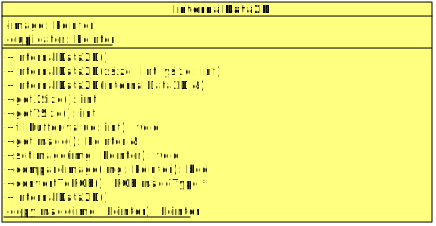
\includegraphics[scale=1]{./Content/Immagini/modelCore/InternalData2D.png}
			\caption{Diagramma classe \textsl{InternalData2D}}
			\label{InternalData2D_img}
\end{figure}

\paragraph{Descrizione\\}
Classe che implementa i contratti definiti da InternalData e rappresenta il formato interno bidimensionale sul quale operare. Implementa il design pattern Adapter e adatta la classe itk::Image della libreria ITK\g{}. Rappresenta la componente Adapter dell'omonimo design pattern\g{}.

\paragraph{Utilizzo \\}
Viene utlizzata nelle feature\g{} come parametro di input da elaborare e rappresenta i signoli canali nelle immagini in formato RGB.

\paragraph{Eredita da:}
	\begin{itemize}
		\item Romeo::Model::Core::InternalData: implementa i contratti di questa classe.
	\end{itemize}

\paragraph{Attributi}
	\begin{itemize}
		\item \color{teal}\verb! - image : ImageType2D::Pointer !\\
		\color{black}
		\subparagraph{Descrizione:} puntatore all'immagine bidimensionale (Tipo ITK\g{}).
		
		\item \color{teal}\verb! - static duplicator : DuplicatorType::Pointer!\\
		\color{black}
		\subparagraph{Desrizione:} \lq\lq{}duplicatore\rq\rq{} delle immagini \textsl{InternalData2D}.
		
	\end{itemize}
	
\paragraph{Metodi}
	\begin{itemize}
		%costruttore default
		\item \color{blue}\verb! + InternalData2D()! \\
		\color{black}
		\subparagraph{Descrizione:} costruttore di \emph{default} della lcasse \textsl{InternalData}.
		
		%costruttore
		\item \color{blue}\verb! + InternalData2D(xSize : int, ySize : int)! \\
		\color{black}
		\subparagraph{Descrizione:} costruttore a due argomenti. Costruisce un immagine di dimensioni \textit{xSize x ySize}. 
		\subparagraph{Argomenti}
			\begin{itemize}
				\item \color{RoyalPurple}\verb!xSize : int! \\ 
				\color{black}Dimensione orizzontale dell'immagine.
				
				\item \color{RoyalPurple}\verb!ySize : int! \\ 
				\color{black}Dimensione verticale dell'immagine.
			\end{itemize}
		
		%costuttore copia
		\item \color{blue}\verb! + InternalData2D(image : const InternalData &)!\\
		\color{black}
		\subparagraph{Descrizione:} costruttore di copia \emph{profondo}.
		\subparagraph{Argomenti}
			\begin{itemize}
				\item \color{RoyalPurple}\verb!image : const InternalData &!\\
				\color{black}Oggetto \textsl{InternalData2D} di cui si vuole fare la copia \emph{profonda}.
			\end{itemize}
		
		\item \color{blue}\verb! + operator=(image : const InternalData2D &) : InternalData2D&!\\
		\color{black}
		\subparagraph{Descrizione:} operatore di assegnazione \emph{profondo}.
		\subparagraph{Argomenti}
			\begin{itemize}
				\item \color{RoyalPurple}\verb!image : const InternalData &!\\
				\color{black}Oggetto \textsl{InternalData2D} di cui si vuole fare la copia \emph{profonda}.
			\end{itemize}
		
		% getXSize
		\item \color{blue}\verb! + getXSize() : int !\\
		\color{black} 
		\subparagraph{Descrizione:} implementa il contratto che ritorna la dimensione orizzontale di un'immagine.
		\subparagraph{Note}
			\begin{itemize}
				\item Il metodo deve essere marcato costante.
			\end{itemize}
		
		% getYSize
		\item \color{blue}\verb! + getYSize() : int !\\
		\color{black}
		\subparagraph{Descrizione:} implementa il contratto che ritorna la dimensione verticale di un'immagine.
		\subparagraph{Note}
			\begin{itemize}
				\item Il metodo deve essere marcato costante.
			\end{itemize}
		
		%fillBuffer
		\item \color{blue}\verb! +  fillBuffer(value : int) : void!\\
		\color{black}
		\subparagraph{Descrizione:} metodo che  \lq\lq{}riempie\rq\rq{} tutti i piexel del colore passato come argomenti.
		\subparagraph{Argomenti}
			\begin{itemize}
				\item \color{blue}\verb!value : int!\\
				\color{black}Rappresenta il colore dell'immagine (0-255). 
			\end{itemize}
		
		%getImage
		\item \color{blue}\verb! + getImage() : ImageType::Pointer& !\\
		\color{black}
		\subparagraph{Descrizione:} ritorna un puntatore ITK\g{} all'immagine rappresentata.
		
		%stImage
		\item \color{blue}\verb! + setImage(img : ImageType::Pointer) : void!\\
		\color{black}
		\subparagraph{Descrizione:} metodo che cambia l'immagine rappresentata dall'oggetto \textsl{InternalData2D}.
		\subparagraph{Argomenti}
			\begin{itemize}
				\item \color{RoyalPurple}\verb!img : ImageType::Pointer!\\
				\color{black}
				Nuova immagine da rappresentare.
			\end{itemize}
			
		\item \color{blue}\verb! + compareImage(img : ImageType::Pointer) : boolean!\\
		\color{black}
		\subparagraph{Descrizione:} metodo che controlla se due immagini sono uguali.
		\subparagraph{Argomenti}
			\begin{itemize}
				\item \color{RoyalPurple}\verb!img : ImageType::Pointer!\\
				\color{black}
				Immagine da confrontare.
			\end{itemize}
		
		%convertToRGB	
		\item \color{blue}\verb! + convertToRGB() : RGBImageType *!\\
		\color{black}
		\subparagraph{Descrizione:} metodo che converte l'oggetto \textsl{InternalData2D} in un oggetto di tipo \textsl{RGBImageType}.
		\subparagraph{Argomenti}
			\begin{itemize}
				\item Il metodo deve essere marcato costante.
			\end{itemize}
			
		% copyImage
		\item \color{blue}\verb! - static copyImage(image : ImageType2D::Pointer) : ImageType2D::Pointer !\\
		\color{black} 
		\subparagraph{Descrizione:} copia un immagine restituendone la copia.
		\subparagraph{Argomenti}
			\begin{itemize}
				\item \color{RoyalPurple}\verb!image : ImageType2D::Pointer!\\
				\color{black}Puntatore di tipo ITK\g{} all'immagine da copiare (tipo ITK\g{}).
			\end{itemize}
		\subparagraph{Note}
			\begin{itemize}
				\item Il metodo deve essere marcato come statico.
			\end{itemize}
			
	\end{itemize}
	
\pagebreak



% % % % % % % % % % % % % % % % % % % % % % % % % % % % % 
% % InternalData3D % % % % % % % % % % % % % % % % % % % % %
% % % % % % % % % % % % % % % % % % % % % % % % % % % % %
\color{black}
\subsubsection{InternalData3D (class)}
\label{InternalData3D}
\begin{figure}[!h]
\centering
			\includegraphics[scale=1]{./Content/Immagini/modelCore/InternalData3D.png}
			\caption{Diagramma Classe \textsl{InternalData3D}}
			\label{InternalData3D_img}
\end{figure}

\paragraph{Descrizione \\}
Classe che rappresenta il formato interno per un'immagine di tipo 3D.
\\Classe che \lq\lq{}adatta\rq\rq{} la classe itk::image fornita dalla libreria esterna ITK\g{}.
\\Rappresenta il componente Adapter del design pattern\g{} Adapter.

\paragraph{Utilizzo \\}
Viene utlizzata nelle feature\g{} come parametro di input da elaborare e rappresenta i signoli canali nelle immagini in formato RGB.

\paragraph{Eredita da:}
\begin{itemize}
	\item InternalData: implementa contratti di questa classe.
\end{itemize}

\paragraph{Attributi \\}
	\begin{itemize}
		\item \color{teal}\verb!- image : ImageType3D::Pointer !
		\color{black}
		\subparagraph{Descrizione:} puntatore all'immagine tridimensionale (Tipo ITK\g{}).
	\end{itemize}
	
\color{black}
\paragraph{Metodi}
	\begin{itemize}
		\item \color{blue}\verb! + InternalData3D()! 
		\color{black} 
		\subparagraph{Descrizione:} costruttore di \emph{default} della classe \textsl{InternalData3D}.

		\item \color{blue}\verb! + InternalData3D(xSize : int, ySize : int, zSize : int)! 
		\color{black} 
		\subparagraph{Descrizione:} costruttore a tre argomenti. Costruisce un immagine tridimensionale \textit{xSize x ySize x zSize}. 
		\subparagraph{Argomenti}
			\begin{itemize}
				\item \color{RoyalPurple}\verb! xSize : int! \\ 
				\color{black}Dimensione orizzontale;
				
				\item \color{RoyalPurple} \verb!ySize : int! \\ 
				\color{black}Dimensione verticale;
				
				\item \color{RoyalPurple}\verb!zSize : int! \\ 
				\color{black}Terza dimensione.
			\end{itemize}
			
		\item \color{blue}\verb! + InternalData3D(image :  RGBImageType::Pointer )!
		\color{black}
		\subparagraph{Descrizione:} costruttore che costriuisce un oggetto \textsl{InternalData3D}.
		\subparagraph{Argomenti}
			\begin{itemize}
				\item \color{RoyalPurple}\verb!image :  RGBImageType::Pointer!\\
				\color{black}Puntatore all'immagine da creare.
			\end{itemize}		
			
		\item \color{blue}\verb!InternalData3D(image : const InternalData3D &)!
		\color{black}
		\subparagraph{Descrizione:} costruttore di copia \emph{profondo}.
		\subparagraph{Argomenti}
			\begin{itemize}
				\item \color{RoyalPurple}\verb!image : const InternalData3D &!\\
				\color{black}Immagine di cui si vuole effettuare la copia.
			\end{itemize}
			
		% getXSize
		\item \color{blue}\verb! + getXSize() : int !\\
		\color{black} 
		\subparagraph{Descrizione:} implementa il contratto che ritorna la dimensione orizzontale di un'immagine.
		\subparagraph{Note}
			\begin{itemize}
				\item Il metodo deve essere marcato costante.
			\end{itemize}
		
		% getYSize
		\item \color{blue}\verb! + getYSize() : int !\\
		\color{black}
		\subparagraph{Descrizione:} implementa il contratto che ritorna la dimensione verticale di un'immagine.
		\subparagraph{Note}
			\begin{itemize}
				\item Il metodo deve essere marcato costante.
			\end{itemize}
			
		% getYSize
		\item \color{blue}\verb! + getZSize() : int !\\
		\color{black}
		\subparagraph{Descrizione:} implementa il contratto che ritorna la terza dimensione di un'immagine.
		\subparagraph{Note}
			\begin{itemize}
				\item Il metodo deve essere marcato costante.
			\end{itemize}
			
	%getImage
	\item \color{blue}\verb! + getImage() : ImageType::Pointer& !\\
	\color{black}
	\subparagraph{Descrizione:} ritorna un puntatore ITK\g{} all'immagine rappresentata.
			
	%stImage
	\item \color{blue}\verb! + setImage(img : ImageType::Pointer) : void!\\
	\color{black}
	\subparagraph{Descrizione:} metodo che cambia l'immagine rappresentata dall'oggetto \textsl{InternalData2D}.
	\subparagraph{Argomenti}
		\begin{itemize}
			\item \color{RoyalPurple}\verb!img : ImageType::Pointer!\\
			\color{black}
			Nuova immagine da rappresentare.
		\end{itemize}
		
		% copyImage
		\item \color{blue}\verb! - static copyImage(image : ImageType2D::Pointer) : ImageType2D::Pointer !\\
		\color{black} 
		\subparagraph{Descrizione:} copia un immagine restituendone la copia.
		\subparagraph{Argomenti}
			\begin{itemize}
				\item \color{RoyalPurple}\verb!image : ImageType2D::Pointer!\\
				\color{black}Puntatore di tipo ITK\g{} all'immagine da copiare (tipo ITK\g{}).
			\end{itemize}
		\subparagraph{Note}
			\begin{itemize}
				\item Il metodo deve essere marcato come statico.
			\end{itemize}
		
	\end{itemize}
	
\pagebreak	
	% % % % % % % % % % % % % % % % % % % % % % % % % % % % % %
	% % RomeoObject % % % % % % % % % % % % % % % % % % % % %
	% % % % % % % % % % % % % % % % % % % % % % % % % % % % % %
	
	\color{black}
	\subsubsection{RomeoObject(interface)}
	\label{romeoobject}
		\begin{figure}[!h]
			\centering
			\includegraphics[scale=1]{./Content/Immagini/modelCore/RomeoObject}
			\caption{Diagramma calsse \textsl{RomeoObject}}
			\label{romeoobject_img}
		\end{figure}
		
	\paragraph{Descrizione\\}
	Intefaccia che rappresenta un generico dato da analizzare in Romeo\g{}.
	
	\paragraph{Utilizzo\\}
	Viene utilizzato nei metodi delle feature e algoritmi per lavorare su un generico dato.
	
	\paragraph{Metodi}
		\begin{itemize}
			\item \color{blue}\verb! + getXSize() : int !\\
			\color{black}
			\subparagraph{Descrione:} contratto che ritorna la dimensione x del dato.
			\subparagraph{Note}
				\begin{itemize}
					\item Il metodo deve essere marcato come costante.
				\end{itemize}
				
				\item \color{blue}\verb! + getYSize() : int !\\
					\color{black}
					\subparagraph{Descrione:} contratto che ritorna la dimensione y del dato.
					\subparagraph{Note}
						\begin{itemize}
							\item Il metodo deve essere marcato come costante.
						\end{itemize}
						
				\item \color{blue}\verb! + maskImage(mask : const QString &) : void!\\
				\color{black}
				\subparagraph{Descrizione:} contratto che applica la maschera ad un dato.
				\subparagraph{Argomenti}
					\begin{itemize}
						\item \color{RoyalPurple}\verb!mask : const QString &!\\
						\color{black}Percorso della maschera\g{} da applicare al dato. 
					\end{itemize}
				
			
		\end{itemize}
		
	
\pagebreak	

% % % % % % % % % % % % % % % % % % % % % % % % % % % % % 
% % RGBImage % % % % % % % % % % % % % % % % % % % % %
% % % % % % % % % % % % % % % % % % % % % % % % % % % % %
\color{black}
\subsubsection{RGBImage (abstract)}
\label{RGBImage}
\begin{figure}[!h]
\centering
			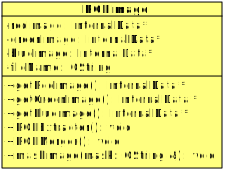
\includegraphics[scale=1]{./Content/Immagini/modelCore/RGBImage.png}
			\caption{Diagramma classe \textsl{RGBImage}}
			\label{RGBImage_img}
\end{figure}

\paragraph{Descrizione \\}
Classe astratta che rappresenta un'immagine RGB, composta da tre livelli di colore \textit{red, green} e \textit{blue}. Definisce dei contratti per l'accesso ai tre livelli di colore, per la loro scomposizione e fusione.

\paragraph{Utilizzo \\}
Viene utilizzata quando una feature\g{}  deve essere applicata ad un immagine e non ad un video.
\\Inoltre viene utilizzata per salvare le informazioni riguardanti il colore dell'immagine, che altrimenti sarebbe in scala di grigi.

\paragraph{Attributi \\}
	\begin{itemize}
		% fileName
		\item \color{teal}\verb!- fileName : QString !
		\color{black} 
		\subparagraph{Descrizione:} nome dell'immagine.
		
		% redimage
		\item \color{teal}\verb!- redImage : InternalDat a* !
		\color{black} Puntatore polimorfo al formato interno rappresentante il livello di rosso di un'immagine.

		% greenimage
		\item \color{teal}\verb!- greenImage : InternalData* !
			\color{black}
			\subparagraph{Descrizione:} puntatore polimorfo al formato interno rappresentante il livello di verde di un'immagine.
			\
			
		% blueimage
		\item \color{teal}\verb!- blueImage : InternalData* !
		\color{black} 
		\subparagraph{Descrizione:} puntatore polimorfo al formato interno rappresentante il livello di blu di un'immagine.

	\end{itemize}

\paragraph{Metodi \\}
	\begin{itemize}
	   % getRedImage
		\item \color{blue}\verb! + getRedImage() : InternalData *! 
		\color{black}
		\subparagraph{Descrizione:} metodo che ritorna il puntatore al formato interno rappresentante il livello di rosso di un'immagine.
	
		% getGreenImage
		\item \color{blue}\verb! + getGreenImage() : InternalData *!
		\color{black} 
		\subparagraph{Descrizione:} metodo che ritorna il puntatore al formato interno rappresentante il livello di verde di un'immagine.
		
		% getBlueImage
		\item \color{blue}\verb! + getBlueImage() : InternalData *! 
		\color{black} 
		\subparagraph{Descrizione;} metodo che ritorna il puntatore al formato interno rappresentante il livello di blu di un'immagine.
		
		
		% RGBExtracter
		\item \color{blue}\verb! + RGBExtracter() : void! 
		\color{black}
		\subparagraph{Descrizione:} contratto che estrae da un'immagine RGB tre formati interni rappresentanti i tre diversi livelli di un'immagine.
		
		% RGBMerger
		\item \color{blue}\verb! + RGBMerger() : void! 
		\color{black}
		\subparagraph{Descrizione:} contratto che ricompone un'immagine RGB ricostruendola dai tre formati interni rappresentanti i tre diversi livelli di un'immagine.
	\end{itemize}

	\pagebreak
% % % % % % % % % % % % % % % % % % % % % % % % % % % % % 
% % RGBImage2D % % % % % % % % % % % % % % % % % % % % %
% % % % % % % % % % % % % % % % % % % % % % % % % % % % %
\color{black}
\subsubsection{RGBImage2D (class)}
\label{RGBImage2D}
\begin{figure}[!h]
\centering
			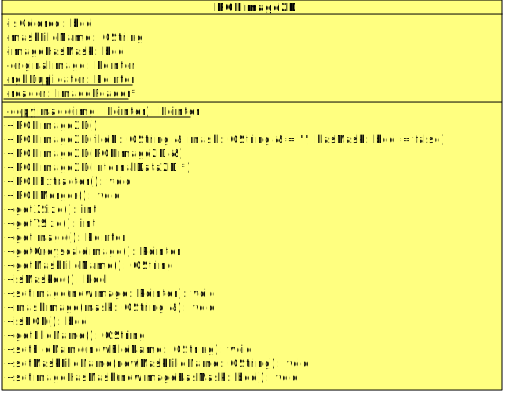
\includegraphics[scale=1]{./Content/Immagini/modelCore/RGBImage2D.png}
			\caption{Diagramma classe \textsl{ RGBImage2D}}
			\label{RGBImage2D_img}
\end{figure}

\paragraph{Descrizione \\}
Classe che rappresenta un immagine bidimensionale, a colori in Romeo\g{}
\\Classe che \lq\lq{}adatta\rq\rq{} la classe itk::image fornita da itk.
\\Rappresenta il componente Adapter del design pattern\g{} Adapter.

\paragraph{Utilizzo \\}
Viene utilizzata dalle feature\g{} che elaborano immagini bidimensionali.
\\Inoltre racchiude in se le informazioni sul colore delle immagini importate 

\paragraph{Eredita da:}
\begin{itemize}
	\item Romeo::Model::Core::RGBImage.
\end{itemize}

\paragraph{Attributi}
	\begin{itemize}
		% originalImage
		\item \color{teal}\verb!- originalImage : RGBImageType::Pointer !\\
		\color{black}
		\subparagraph{Descrizione:} puntatore all'immagine.
		
		%iscolored
		\item \color{teal}\verb! -isColored : boolean!\\
		\color{black}
		\subparagraph{Descrizione:} booleano che indica se l'immagine è colorata o a scala di grigi.
		
		%maskFileName
		\item \color{teal}\verb! - maskFileName : QString!\\
		\color{black}
		\subparagraph{Descrizione:} percorseo della maschera\g{} dell'immagine.
		
		\item \color{teal}\verb! - imageHasMask : boolean!\\
		\color{black}
		\subparagraph{Descrizione:} booelano che indica se l'immagine ha una maschera o no.
		
		\item \color{teal}\verb! -static rgbDuplicator : DuplicatorType::Pointer !\\
		\color{black}
		\subparagraph{Descrizione:} duplicatore per un immagine di tipo \textsl{RGBImage2D}.
		
		\item \color{teal}\verb! - static  reader : ImageReader*!
		\color{black}
		\subparagraph{Descrizione:} reader pr un'immagine di tipo \textsl{RGBImage2D}.
		

	\end{itemize}

\color{black}
\paragraph{Metodi }
	\begin{itemize}
	 %RGBImage2D
		\item \color{blue}\verb! + RGBImage2D()! \\
		\color{black} Costruttore di \emph{default} della classe \textsl{RGBImage2D}.
		
		% RGBImage2D
		\item \color{blue}\verb! + RGBImage2D(fileName : const QString &,  mask ; const QString&,!\\
								   \verb!hasMask : boolean)! 
			\color{black} 
			\subparagraph{Descrizione:} costruttore a tre argomenti della classe \textsl{RGBImage2D}.	
			\subparagraph{Argomenti}
			\begin{itemize}
				\item \color{RoyalPurple}\verb!fileName : QString &! \\
				\color{black}Percorso dell'immagine da caricare. Verrà passato al \textit{ReaderImage} che caricherà l'immagine.
			\end{itemize}
			
		\item \color{blue}\verb! + RGBImage2D(image : const RGBImage2D &)!\\
		\color{black}
		\subparagraph{Descrizione:} costruttore di copia \emph{profondo}.
		\subparagraph{Argomenti:}
			\begin{itemize}
				\item \color{RoyalPurple}\verb!image : const RGBImage2D &)!\\
				\color{black}Immagine di cui si vuole fare la copia.
			\end{itemize}
		
		\item \color{blue}\verb! + RGBImage2D(image : InternalData2D*)!\\
		\color{black}
		\subparagraph{Descrizione:} costruisce un'immagine \textsl{RGBImage2D} a partire da un oggetto \textsl{InternalData2D}.
		\subparagraph{Argomenti}
			\begin{itemize}
				\item \color{RoyalPurple}\verb!image : InternalData2D*!\\
				\color{black}Oggetto \textsl{InternalData2D} da cui si vuole ricavare l'oggetto \textsl{RGBImage2D}.
			\end{itemize}
			
	% RGBExtracter
		\item \color{blue}\verb! + RGBExtracter() : void! 
		\color{black}
		\subparagraph{Descrizione:} metodo che estrae da un'immagine RGB tre formati interni rappresentanti i tre diversi livelli di un'immagine.
		
		% RGBMerger
		\item \color{blue}\verb! + RGBMerger() : void! 
		\color{black}
		\subparagraph{Descrizione:} metodo che ricompone un'immagine RGB ricostruendola dai tre formati interni rappresentanti i tre diversi livelli di un'immagine.
		
	% getXSize
	\item \color{blue}\verb! + getXSize() : int !\\
	\color{black}
	\subparagraph{Descrizione: } ritorna la dimensione orizzontale dell'immagine.
	\subparagraph{Note}
		\begin{itemize}
			\item Il metodo deve essere marcato come costante.
		\end{itemize}
		
	% getYSize
	\item \color{blue}\verb! + getYSize() : int !\\
	\color{black}
	\subparagraph{Descrizione: } ritorna la dimensione verticale dell'immagine.
	\subparagraph{Note}
		\begin{itemize}
			\item Il metodo deve essere marcato come costante.
		\end{itemize}
		
	\item \color{blue}\verb! +  getImage() : RGBImageType::Pointer!\\
	\color{black}
	\subparagraph{Descrizione:} metodo che ritorna un puntatore ITK\g{} all'immagine.
	
	\item \color{blue}\verb! + getGreyscaleImage() : ImageType::Pointer!\\
	\color{black}
	\subparagraph{Descrizione:} metodo che ritorna un puntatore ITK\g{} all'immagine rappresentata come scala di grigi.
	
	\item \color{blue}\verb! + getMaskFileName() : QString!\\
	\color{black}
	\subparagraph{Descrizione:} metodo che ritorna il percorso dell'eventuale maschera\g{} dell'immagine.
	\subparagraph{Note}
		\begin{itemize}
			\item Il metodo deve essere marcato costante.
		\end{itemize}
		
	\item \color{blue}\verb! + isMasked() : boolean!\\
	\color{black}
	\subparagraph{Descrizione:} metodo che ritorna un booelano indicante se l'immagine ha una maschera o meno.
	\subparagraph{Note}
			\begin{itemize}
				\item Il metodo deve essere marcato costante.
			\end{itemize}
	
	\item \color{blue}\verb! + setImage(newImage : RGBImageType::Pointer ) : void!\\
	\color{black}
	\subparagraph{Descrizione:} metodo che cambia l'immagine rappresentata.
	\subparagraph{Argomeni}
		\begin{itemize}
			\item \color{RoyalPurple}\verb!newImage : RGBImageType::Pointer!\\
			\color{black}Puntatore ITK\g{} alla nuova immagine.
		\end{itemize}
		
	\item \color{blue}\verb! + maskImage(mask : const QString &) : void!\\
	\color{black}
	\subparagraph{Descrizione:} metodo che applica la maschera ad un immagine \textsl{RGBImage2D}.
	\subparagraph{Argomenti}
		\begin{itemize}
			\item \color{RoyalPurple}\verb!mask : const QString &!\\
			\color{black}Percorso della maschera\g{} da applicare all'oggetto \textsl{RGBImage2D}. 
		\end{itemize}
		
	\item \color{blue}\verb! + isRGB() : boolean!\\
	\color{black}
	\subparagraph{Descrizione:} metodo che ritorna un booleano indicante se l'immagine è RGB o no.
	\subparagraph{Argomenti}
		\begin{itemize}
			\item Il metodo deve essere marcato costante.
		\end{itemize}
	\subparagraph{Note}
			\begin{itemize}
				\item Il metodo deve essere marcato come costante.
			\end{itemize}
	
	\item \color{blue}\verb! + getFileName() : QString!\\
	\color{black}
	\subparagraph{Descrizione:} metodo che ritorna il nome del file rappresentato.
	\subparagraph{Note}
		\begin{itemize}
			\item Il metodo deve essere marcato come costante.
		\end{itemize}
	
	\item \color{blue}\verb! + setFileName(newFileName : QString ) : void!\\
	\color{black}
	\subparagraph{Descrizione:} metodo che cambia il file rappresentato.
	\subparagraph{Argomenti}
		\begin{itemize}
			\item \color{RoyalPurple}\verb!newFileName : QString !\\
			\color{black}Nuovo file da rappresentato.
		\end{itemize}
		
	\item \color{blue}\verb! + setMaskFileName(newMaskFileName : QString) : void!\\
	\color{black}
	\subparagraph{Descrizione:} metodo che cambia la maschera\g{} dell'immagine rappresentata.
	\subparagraph{Argomenti}
		\begin{itemize}
			\item \color{RoyalPurple}\verb!newMaskFileName : QString!\\
			\color{black}Nuova maschera.
		\end{itemize}
	  
	 \item \color{blue}\verb! +setImageHasMask(newImageHasMask : bool ) : void!\\
	  \color{black}
	  \subparagraph{Descrizione:} assegna all'attributo \verb!imageHasMask! un nuovo valore.
	  \subparagraph{Argomenti}
	  	\begin{itemize}
		  	\item \color{RoyalPurple}\verb!newImageHasMask : bool!\\
		  	\color{black}Il nuovo valore.
	  	\end{itemize}
		
		
	\end{itemize}
\pagebreak
% % % % % % % % % % % % % % % % % % % % % % % % % % % % % 
% % RGBImage3D % % % % % % % % % % % % % % % % % % % % %
% % % % % % % % % % % % % % % % % % % % % % % % % % % % %
\color{black}
\subsubsection{RGBImage3D (class)}
\label{RGBImage3D}
\begin{figure}[!h]
\centering
			\includegraphics[scale=1]{./Content/Immagini/modelCore/RGBImage3D.png}
			\caption{Diagramma classe \textsl{RGBImage3D}}
			\label{RGBImage3D_img}
\end{figure}

\paragraph{Descrizione \\}
Classe che concretizza RGBImage e rappresenta un'immagine RGB tridimensionale, composta da tre livelli di colore \textit{red, green} e \textit{blue}. Implementa i contratti per l'accesso ai tre livelli di colore, per la loro scomposizione e fusione.
Utilizza il template itk::Image della libreria ITK\g{} per rappresentare l'immagine.

\paragraph{Utilizzo \\}
Viene utilizzata dalle sottoclassi di AFeature e di AAlgorithm per applicare le varie feature\g{} e algoritmi di clustering\g{}.

\paragraph{Eredita da:}
\begin{itemize}
	\item Romeo::Model::Core::RGBImage.
\end{itemize}

\paragraph{Attributi}
	\begin{itemize}
		% originalImage
		\item \color{teal}\verb!- originalImage : RGBImageType::Pointer !\\
		\color{black}
		\subparagraph{Descrizione:} puntatore all'immagine.
		
		
		
		%maskFileName
		\item \color{teal}\verb! - maskFileName : QString!\\
		\color{black}
		\subparagraph{Descrizione:} percorseo della maschera\g{} dell'immagine.
		
		\item \color{teal}\verb! - imageHasMask : boolean!\\
		\color{black}
		\subparagraph{Descrizione:} booelano che indica se l'immagine ha una maschera o no.
		
		\item \color{teal}\verb! - static  reader : ImageReader*!
		\color{black}
		\subparagraph{Descrizione:} reader pr un'immagine di tipo \textsl{RGBImage3D}.
		

	\end{itemize}

\color{black}
\paragraph{Metodi }
	\begin{itemize}
	 %RGBImage2D
		\item \color{blue}\verb! + RGBImage3D()! \\
		\color{black} Costruttore di \emph{default} della classe \textsl{RGBImage3D}.
		
		% RGBImage2D
		\item \color{blue}\verb! + RGBImage3D(fileName : const QString &,  mask ; const QString&,!\\
								   \verb!hasMask : boolean)! 
			\color{black} 
			\subparagraph{Descrizione:} costruttore a tre argomenti della classe \textsl{RGBImage3D}.	
			\subparagraph{Argomenti}
			\begin{itemize}
				\item \color{RoyalPurple}\verb!fileName : QString &! \\
				\color{black}Percorso dell'immagine da caricare. Verrà passato al \textit{ReaderImage} che caricherà l'immagine.
			\end{itemize}
			
		\item \color{blue}\verb! + RGBImage3D(image : const RGBImage3D &)!\\
		\color{black}
		\subparagraph{Descrizione:} costruttore di copia \emph{profondo}.
		\subparagraph{Argomenti:}
			\begin{itemize}
				\item \color{RoyalPurple}\verb!image : const RGBImag3D &)!\\
				\color{black}Immagine di cui si vuole fare la copia.
			\end{itemize}
		
		\item \color{blue}\verb! + RGBImage3D(image : InternalData3D*)!\\
		\color{black}
		\subparagraph{Descrizione:} costruisce un'immagine \textsl{RGBImage3D} a partire da un oggetto \textsl{InternalData3D}.
		\subparagraph{Argomenti}
			\begin{itemize}
				\item \color{RoyalPurple}\verb!image : InternalData3D*!\\
				\color{black}Oggetto \textsl{InternalDat3D} da cui si vuole ricavare l'oggetto \textsl{RGBImage3D}.
			\end{itemize}
			
	% RGBExtracter
		\item \color{blue}\verb! + RGBExtracter() : void! 
		\color{black}
		\subparagraph{Descrizione:} metodo che estrae da un'immagine RGB tre formati interni rappresentanti i tre diversi livelli di un'immagine.
		
		% RGBMerger
		\item \color{blue}\verb! + RGBMerger() : void! 
		\color{black}
		\subparagraph{Descrizione:} metodo che ricompone un'immagine RGB ricostruendola dai tre formati interni rappresentanti i tre diversi livelli di un'immagine.
		
	% getXSize
	\item \color{blue}\verb! + getXSize() : int !\\
	\color{black}
	\subparagraph{Descrizione: } ritorna la dimensione orizzontale dell'immagine.
	\subparagraph{Note}
		\begin{itemize}
			\item Il metodo deve essere marcato come costante.
		\end{itemize}
		
	% getYSize
	\item \color{blue}\verb! + getYSize() : int !\\
	\color{black}
	\subparagraph{Descrizione: } ritorna la dimensione verticale dell'immagine.
	\subparagraph{Note}
		\begin{itemize}
			\item Il metodo deve essere marcato come costante.
		\end{itemize}
	
	%getZSize
	\item \color{blue}\verb! + getZSize() : int!\\
	\color{black}
	\subparagraph{Descrizione:} ritorna la terza  dimensione dell'immagine.
	\subparagraph{Note}
		\begin{itemize}
			\item Il metodo deve essere marcato come costante.
		\end{itemize}
		
	\item \color{blue}\verb! +  getImage() : RGBImageType::Pointer!\\
	\color{black}
	\subparagraph{Descrizione:} metodo che ritorna un puntatore ITK\g{} all'immagine.
	
	\item \color{blue}\verb! + getGreyscaleImage() : ImageType::Pointer!\\
	\color{black}
	\subparagraph{Descrizione:} metodo che ritorna un puntatore ITK\g{} all'immagine rappresentata come scala di grigi.
	
	\item \color{blue}\verb! + getMaskFileName() : QString!\\
	\color{black}
	\subparagraph{Descrizione:} metodo che ritorna il percorso dell'eventuale maschera\g{} dell'immagine.
	\subparagraph{Note}
		\begin{itemize}
			\item Il metodo deve essere marcato costante.
		\end{itemize}
		
	\item \color{blue}\verb! + isMasked() : boolean!\\
	\color{black}
	\subparagraph{Descrizione:} metodo che ritorna un booelano indicante se l'immagine ha una maschera o meno.
	\subparagraph{Note}
			\begin{itemize}
				\item Il metodo deve essere marcato costante.
			\end{itemize}
	
	\item \color{blue}\verb! + setImage(newImage : RGBImageType::Pointer ) : void!\\
	\color{black}
	\subparagraph{Descrizione:} metodo che cambia l'immagine rappresentata.
	\subparagraph{Argomeni}
		\begin{itemize}
			\item \color{RoyalPurple}\verb!newImage : RGBImageType::Pointer!\\
			\color{black}Puntatore ITK\g{} alla nuova immagine.
		\end{itemize}
		
	\item \color{blue}\verb! + maskImage(mask : const QString &) : void!\\
	\color{black}
	\subparagraph{Descrizione:} metodo che applica la maschera ad un immagine \textsl{RGBImage3D}.
	\subparagraph{Argomenti}
		\begin{itemize}
			\item \color{RoyalPurple}\verb!mask : const QString &!\\
			\color{black}Percorso della maschera\g{} da applicare all'oggetto \textsl{RGBImage3D}. 
		\end{itemize}
		
	\item \color{blue}\verb! + isRGB() : boolean!\\
	\color{black}
	\subparagraph{Descrizione:} metodo che ritorna un booleano indicante se l'immagine è RGB o no.
	\subparagraph{Argomenti}
	\subparagraph{Note}
			\begin{itemize}
				\item Il metodo deve essere marcato come costante.
			\end{itemize}
	
	\item \color{blue}\verb! + getFileName() : QString!\\
	\color{black}
	\subparagraph{Descrizione:} metodo che ritorna il nome del file rappresentato.
	\subparagraph{Note}
		\begin{itemize}
			\item Il metodo deve essere marcato come costante.
		\end{itemize}
	
	\item \color{blue}\verb! + setFileName(newFileName : QString ) : void!\\
	\color{black}
	\subparagraph{Descrizione:} metodo che cambia il file rappresentato.
	\subparagraph{Argomenti}
		\begin{itemize}
			\item \color{RoyalPurple}\verb!newFileName : QString !\\
			\color{black}Nuovo file da rappresentato.
		\end{itemize}
		
	\item \color{blue}\verb! + setMaskFileName(newMaskFileName : QString) : void!\\
	\color{black}
	\subparagraph{Descrizione:} metodo che cambia la maschera\g{} dell'immagine rappresentata.
	\subparagraph{Argomenti}
		\begin{itemize}
			\item \color{RoyalPurple}\verb!newMaskFileName : QString!\\
			\color{black}Nuova maschera.
		\end{itemize}
	  
	 \item \color{blue}\verb! +setImageHasMask(newImageHasMask : bool ) : void!\\
	  \color{black}
	  \subparagraph{Descrizione:} assegna all'attributo \verb!imageHasMask! un nuovo valore.
	  \subparagraph{Argomenti}
	  	\begin{itemize}
		  	\item \color{RoyalPurple}\verb!newImageHasMask : bool!\\
		  	\color{black}Il nuovo valore.
	  	\end{itemize}
	
	\end{itemize}

% % % % % % % % % % % % % % % % % % % % % % % % % % % % % 
% % Video % % % % % % % % % % % % % % % % % % % % %
% % % % % % % % % % % % % % % % % % % % % % % % % % % % %
\pagebreak
\subsubsection{Video(abstract)}
\label{Video}
\begin{figure}[!h]
\centering
			\includegraphics[scale=1]{./Content/Immagini/modelCore/Video.png}
			\caption{Diagramma classe \textsl{Video}}
			\label{RGBVideo_img}
\end{figure}

\paragraph{Descrizione \\}
Classe astratta che rappresenta la classe base di tutti i video in Romeo\g{}.
\\È composta da un vettore di oggetti di tipo \textsl{InternalData}.

\paragraph{Utilizzo \\}
viene utilizzata dalle Feature\g{} dinamiche quando ci si aspetta un video generico.

\paragraph{Attributi\\}
	\begin{itemize}
		\item  \color{teal}\verb! # fileName : QString!\\
		\color{black}
		\subparagraph{Descrizione:} percorso del video.
		 
		 \item \color{teal}\verb! # static reader : VideoReader *!\\
		 \color{black}
		 \subparagraph{Descrizione:} puntatore al reader dei video.
		 
		 \item \color{teal}\verb! -originalVideo : QVector<InternalData *>!\\
		 \color{black}
		 \subparagraph{Descrizione:} vettore di frames del video.
	\end{itemize}
	
\paragraph{Metodi\\}
	\begin{itemize}
		\item \color{blue}\verb! + Video(name : const QStirng &)!\\
			\color{black}
			\subparagraph{Descrizione:} costruttore della classe.
			\subparagraph{Argomenti}
				\begin{itemize}
					\item \color{RoyalPurple}\verb!name : const QStirng &!\\
					\color{black}Percorso del video.
				\end{itemize}
			
		\item \color{blue}\verb! + getXSize() : int !\\
		\color{black}
		\subparagraph{Descrizione:} metodo che ritorna la larghezza del frame video.
		\subparagraph{Note}
			\begin{itemize}
				\item Il metodo deve essere marcato come costante.
			\end{itemize}
		
		\item \color{blue}\verb! + getYSize() : int !\\
		\color{black}
		\subparagraph{Descrizione:} metodo che ritorna l'altezza del frame video.
		\subparagraph{Note}
			\begin{itemize}
				\item Il metodo deve essere marcato come costante.
			\end{itemize}
			
		\item \color{blue}\verb! + getNumberOfFrames() : int !\\
		\color{black}
		\subparagraph{Descrizione:} metodo che ritorna il numero di frame presenti nel video.
		\subparagraph{Note}
			\begin{itemize}
				\item Il metodo deve essere marcato come costante.
			\end{itemize}
			
		\item \color{blue}\verb! + getFrame(i : int) : InternalData * !\\
		\color{black}
		\subparagraph{Descrizione:} metodo che ritorna il frame i-esimo del video.
		\subparagraph{Argomenti}
				\begin{itemize}
					\item \color{RoyalPurple}\verb!i : int !\\
					\color{black}Indice del frame da ottenere.
				\end{itemize}
		
		\item \color{blue}\verb! + maskImage(mask : QString &) : void !\\
		\color{black}
		\subparagraph{Descrizione:} metodo che aggiunge una maschera ad un video.
		\subparagraph{Argomenti}
				\begin{itemize}
					\item \color{RoyalPurple}\verb!mask : QString & !\\
					\color{black}Percorso della maschera nel filesystem.
				\end{itemize}
		
	\end{itemize}
	
% % % % % % % % % % % % % % % % % % % % % % % % % % % % % 
% % Video2D % % % % % % % % % % % % % % % % % % % % % % %
% % % % % % % % % % % % % % % % % % % % % % % % % % % % %
\pagebreak
\subsubsection{Video2D(class)}
\label{Video2D}
\begin{figure}[!h]
\centering
			\includegraphics[scale=1]{./Content/Immagini/modelCore/Video2D.png}
			\caption{Diagramma classe \textsl{Video2D}}
			\label{Video2D_img}
\end{figure}

\paragraph{Descrizione \\}
Classe che rappresenta un video bidimensionale in Romeo\g{}.
\\È composta da un vettore di oggetti di tipo \textsl{InternalData2D}.

\paragraph{Utilizzo \\}
viene utilizzata dalle Feature\g{} dinamiche quando ci si aspetta un video bidimensionale.

\paragraph{Metodi\\}
	\begin{itemize}
		\item \color{blue}\verb! + Video2D(fileN : const QString& fileN, mask : const QString & , hasMask : bool)!\\
			\color{black}
			\subparagraph{Descrizione:} costruttore della classe.
			\subparagraph{Argomenti}
				\begin{itemize}
					\item \color{RoyalPurple}\verb!fileN : const QStirng &!\\
					\color{black}Percorso del video nel filesystem.
					\item \color{RoyalPurple}\verb!mask : const QStirng &!\\
					\color{black}Percorso della maschera del video nel filesystem.
					\item \color{RoyalPurple}\verb!hasMask : bool!\\
					\color{black} true se il video possiede una maschera.
				\end{itemize}
				
		\item \color{blue}\verb! + getXSize() : int !\\
		\color{black}
		\subparagraph{Descrizione:} metodo che ritorna la larghezza del frame video.
		\subparagraph{Note}
			\begin{itemize}
				\item Il metodo deve essere marcato come costante.
			\end{itemize}
		
		\item \color{blue}\verb! + getYSize() : int !\\
		\color{black}
		\subparagraph{Descrizione:} metodo che ritorna l'altezza del frame video.
		\subparagraph{Note}
			\begin{itemize}
				\item Il metodo deve essere marcato come costante.
			\end{itemize}
			
		\item \color{blue}\verb! + getNumberOfFrames() : int !\\
		\color{black}
		\subparagraph{Descrizione:} metodo che ritorna il numero di frame presenti nel video.
		\subparagraph{Note}
			\begin{itemize}
				\item Il metodo deve essere marcato come costante.
			\end{itemize}
			
		\item \color{blue}\verb! + getFrame(i : int) : InternalData2D * !\\
		\color{black}
		\subparagraph{Descrizione:} metodo che ritorna il frame i-esimo del video.
		\subparagraph{Argomenti}
				\begin{itemize}
					\item \color{RoyalPurple}\verb!i : int !\\
					\color{black}Indice del frame da ottenere.
				\end{itemize}
		
		\item \color{blue}\verb! + maskImage(mask : QString &) : void !\\
		\color{black}
		\subparagraph{Descrizione:} metodo che aggiunge una maschera ad un video.
		\subparagraph{Argomenti}
				\begin{itemize}
					\item \color{RoyalPurple}\verb!mask : QString & !\\
					\color{black}Percorso della maschera nel filesystem.
				\end{itemize}
				
	\end{itemize}
	
% % % % % % % % % % % % % % % % % % % % % % % % % % % % % 
% % Video3D % % % % % % % % % % % % % % % % % % % % % % %
% % % % % % % % % % % % % % % % % % % % % % % % % % % % %
\pagebreak
\subsubsection{Video3D(class)}
\label{Video3D}
\begin{figure}[!h]
\centering
			\includegraphics[scale=1]{./Content/Immagini/modelCore/Video3D.png}
			\caption{Diagramma classe \textsl{Video3D}}
			\label{Video3D_img}
\end{figure}

\paragraph{Descrizione \\}
Classe che rappresenta un video tridimensionale in Romeo\g{}.
\\È composta da un vettore di oggetti di tipo \textsl{InternalData2D}.

\paragraph{Utilizzo \\}
Viene utilizzata dalle Feature\g{} dinamiche quando ci si aspetta un video tridimensionale.

\paragraph{Metodi\\}
	\begin{itemize}
		\item \color{blue}\verb! + Video2D(fileN : const QString& fileN, mask : const QString & , hasMask : bool)!\\
			\color{black}
			\subparagraph{Descrizione:} costruttore della classe.
			\subparagraph{Argomenti}
				\begin{itemize}
					\item \color{RoyalPurple}\verb!fileN : const QStirng &!\\
					\color{black}Percorso del video nel filesystem.
					\item \color{RoyalPurple}\verb!mask : const QStirng &!\\
					\color{black}Percorso della maschera del video nel filesystem.
					\item \color{RoyalPurple}\verb!hasMask : bool!\\
					\color{black} true se il video possiede una maschera.
				\end{itemize}
				
		\item \color{blue}\verb! + getXSize() : int !\\
		\color{black}
		\subparagraph{Descrizione:} metodo che ritorna la larghezza del frame video.
		\subparagraph{Note}
			\begin{itemize}
				\item Il metodo deve essere marcato come costante.
			\end{itemize}
		
		\item \color{blue}\verb! + getYSize() : int !\\
		\color{black}
		\subparagraph{Descrizione:} metodo che ritorna l'altezza del frame video.
		\subparagraph{Note}
			\begin{itemize}
				\item Il metodo deve essere marcato come costante.
			\end{itemize}
		
		\item \color{blue}\verb! + getZSize() : int !\\
		\color{black}
		\subparagraph{Descrizione:} metodo che ritorna la profondità del frame video.
		\subparagraph{Note}
			\begin{itemize}
				\item Il metodo deve essere marcato come costante.
			\end{itemize}
			
		\item \color{blue}\verb! + getNumberOfFrames() : int !\\
		\color{black}
		\subparagraph{Descrizione:} metodo che ritorna il numero di frame presenti nel video.
		\subparagraph{Note}
			\begin{itemize}
				\item Il metodo deve essere marcato come costante.
			\end{itemize}
			
		\item \color{blue}\verb! + getFrame(i : int) : InternalData3D * !\\
		\color{black}
		\subparagraph{Descrizione:} metodo che ritorna il frame i-esimo del video.
		\subparagraph{Argomenti}
				\begin{itemize}
					\item \color{RoyalPurple}\verb!i : int !\\
					\color{black}Indice del frame da ottenere.
				\end{itemize}
		
		\item \color{blue}\verb! + maskImage(mask : QString &) : void !\\
		\color{black}
		\subparagraph{Descrizione:} metodo che aggiunge una maschera ad un video.
		\subparagraph{Argomenti}
				\begin{itemize}
					\item \color{RoyalPurple}\verb!mask : QString & !\\
					\color{black}Percorso della maschera nel filesystem.
				\end{itemize}
				
	\end{itemize}

	\pagebreak
\subsection{Specifica componenti Model::Core::Algorithm}
\label{specificaModelCoreAlgorithm}

\begin{figure}[!h]
\centering
			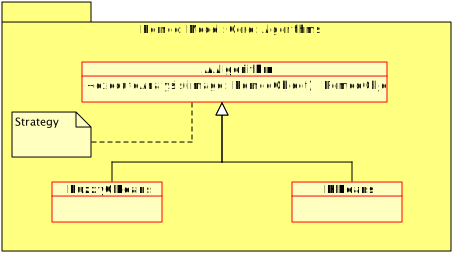
\includegraphics[scale=1]{../Specifica_Tecnica/Content/Immagini/Romeo__Model__Core__Adapters__Algorithms.png}
			\caption{Componente Romeo::Model::Core::Algorithm}
			\label{romeo_model_core}
\end{figure}

Package\g{} contenente le classi per gli algoritmi di clustering\g{}.
% % % % % % % % % % % % % % % % % % % % % %
% % % % AAlgorithm
% % % % % % % % % % % % % % % % % % % %
\subsubsection{AAlgorithm (abstract)}
\label{aalgorithm}
\begin{figure}[!h]
\centering
			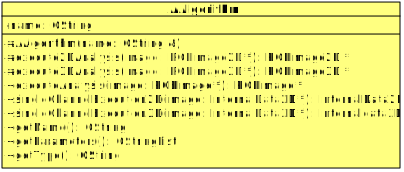
\includegraphics[scale=1]{./Content/Immagini/modelCore/AAlgorithm.png}
			\caption{Diagramma classe \textsl{AAlgorithm}}
			\label{aalgorithm_img}
\end{figure}

\paragraph{Descrizione \\} Classe astratta che rappresenta un generico algoritmo di clustering\g{}, secondo il design pattern Strategy. Definisce dei contratti per l'esecuzione degli algoritmi, che dovranno essere implementati dalle sue sottoclassi.

\paragraph{Utilizzo\\} Fornisce i metodi per l'esecuzione di un algoritmo di clustering su un immagine bidimensionale o tridimensionale.

\paragraph{Attributi\\}
	\begin{itemize}
		\item  \color{teal}\verb! - name : QString !\\
		\color{black}
		\subparagraph{Descrizione:} nome dell'algoritmo.
		\item  \color{teal}\verb! - id : int !\\
		\color{black}
		\subparagraph{Descrizione:} codice identificativo dell'algoritmo.
	\end{itemize}
	
\paragraph{Metodi\\}
	\begin{itemize}
		\item \color{blue}\verb! # execute2DAnalysis(image :RGBImage2D*) : RomeoObject* !\\
			\color{black}
			\subparagraph{Descrizione:} metodo che esegue l'algoritmo di clustering su un immagine bidimensionale.
			\subparagraph{Argomenti}
				\begin{itemize}
					\item \color{RoyalPurple}\verb!image : RGBImage2D*!\\
					\color{black} immagine bidimensionale su cui eseguire l'algoritmo di clustering.
				\end{itemize}
				\subparagraph{Note}
				\begin{itemize}
					\item il metodo deve essere marcato virtuale puro.
				\end{itemize}
				
		\item \color{blue}\verb! # execute3DAnalysis(image :RGBImage3D*) : RomeoObject* !\\
			\color{black}
			\subparagraph{Descrizione:} metodo che esegue l'algoritmo di clustering su un immagine tridimensionale.
			\subparagraph{Argomenti}
				\begin{itemize}
					\item \color{RoyalPurple}\verb!image : RGBImage3D*!\\
					\color{black} immagine tridimensionale su cui eseguire l'algoritmo di clustering.
				\end{itemize}
				\subparagraph{Note}
				\begin{itemize}
					\item il metodo deve essere marcato virtuale puro.
				\end{itemize}
				
		\item \color{blue}\verb! # execute2DVideoAnalysis(video :Video2D*) : RomeoObject* !\\
			\color{black}
			\subparagraph{Descrizione:} metodo che esegue l'algoritmo di clustering su un video bidimensionale.
			\subparagraph{Argomenti}
				\begin{itemize}
					\item \color{RoyalPurple}\verb!video ; Video2D* !\\
					\color{black} video bidimensionale su cui eseguire l'algoritmo di clustering.
				\end{itemize}
				\subparagraph{Note}
				\begin{itemize}
					\item il metodo deve essere marcato virtuale puro.
				\end{itemize}
		\item \color{blue}\verb! # execute3DVideoAnalysis(video : Video3D*) : RomeoObject* !\\
			\color{black}
			\subparagraph{Descrizione:} metodo che esegue l'algoritmo di clustering su un video tridimensionale.
			\subparagraph{Argomenti}
				\begin{itemize}
					\item \color{RoyalPurple}\verb!image : RGBImage2D*!\\
					\color{black} video tridimensionale su cui eseguire l'algoritmo di clustering.
				\end{itemize}
				\subparagraph{Note}
			\begin{itemize}
				\item il metodo deve essere marcato virtuale puro.
			\end{itemize}
			
		\item \color{blue}\verb! + AAlgorithm(algorithmName : const QString& ,algorithmId : int)!\\
			\color{black}
			\subparagraph{Descrizione:} costruttore della classe.
			\subparagraph{Argomenti}
				\begin{itemize}
					\item \color{RoyalPurple}\verb!algorithmName : const QString& !\\
					\color{black} nome dell'algoritmo.
					\item \color{RoyalPurple}\verb!algorithmId : int!\\
					\color{black} codice identificativo dell'algoritmo.
				\end{itemize}
			
	\item \color{blue}\verb! + getParameters() : QStringList!
		\color{black}
		\subparagraph{Descrizione:} metodo che ritorna la lista dei parametri dell'algoritmo di clustering\g{} .
		\subparagraph{Note}
			\begin{itemize}
				\item il metodo deve essere marcato virtuale.
				\item il metodo deve essere marcato cost.
			\end{itemize}
			
	\item \color{blue}\verb! + setParameters(params : const QStringList &) : void!
		\color{black}
		\subparagraph{Descrizione:} inserisce i parametri dell'algoritmo di clustering\g{}.
		\subparagraph{Argomenti}
			\begin{itemize}
				\item \color{RoyalPurple} \verb!params : const QStringList & ! \\ 
				\color{black} lista di parametri dell'algoritmo di clustering\g{}..		
			\end{itemize}
		\subparagraph{Note}
			\begin{itemize}
				\item il metodo deve essere marcato virtuale.
			\end{itemize}
			
	\item \color{blue}\verb! + getName() : QString!
		\color{black}
		\subparagraph{Descrizione:} metodo che ritorna il nome dell'algoritmo di clustering\g{} .
		\subparagraph{Note}
			\begin{itemize}
				\item il metodo deve essere marcato virtuale.
				\item il metodo deve essere marcato cost.
			\end{itemize}
			
	\item \color{blue}\verb! + getId() :int!
		\color{black}
		\subparagraph{Descrizione:} metodo che ritorna il codice identificativo dell'algoritmo di clustering\g{} .
		\subparagraph{Note}
			\begin{itemize}
				\item il metodo deve essere marcato cost.
			\end{itemize}
				
	\item \color{blue}\verb! + setId(i : int) : void!
		\color{black}
		\subparagraph{Descrizione:} inserisce il codice identificativo dell'algoritmo di clustering\g{}.
		\subparagraph{Argomenti}
			\begin{itemize}
				\item \color{RoyalPurple} \verb!i : int ! \\ 
				\color{black} codice identificativo dell'algoritmo di clustering\g{}..		
			\end{itemize}
		
			
	\item \color{blue}\verb! + executeAnalysis(image : RomeoObject* ) : RomeoObject*!
		\color{black}
		\subparagraph{Descrizione:} esegue l'algoritmo di clustering\g{} su un generico dato.
		\subparagraph{Argomenti}
			\begin{itemize}
				\item \color{RoyalPurple} \verb!image : RomeoObject* ! \\ 
				\color{black} generico dato su cui applicare l'algoritmo di clustering\g{}..		
			\end{itemize}
			
	\item \color{blue}\verb! + AAlgorithm()!
		\color{black}
		\subparagraph{Descrizione:} costruttore di default.
			
	\item \color{blue}\verb! + getParametersTypeList()  : QMap<QString, QList<int> >!
		\color{black}
		\subparagraph{Descrizione:} metodo che ritorna la lista dei parametri di tipo dell'algoritmo di clustering\g{} .
		\subparagraph{Note}
			\begin{itemize}
				\item il metodo deve essere marcato virtuale puro.
				\item il metodo deve essere marcato costante.
			\end{itemize}	
			
	\item \color{blue}\verb! + getParametersOfTypeChoice()  : QVector< QMap<char, QString> >!
		\color{black}
		\subparagraph{Descrizione:} metodo che ritorna la lista dei parametri di scelta dell'algoritmo di clustering\g{} .
		\subparagraph{Note}
			\begin{itemize}
				\item il metodo deve essere marcato virtuale.
				\item il metodo deve essere marcato costante.
			\end{itemize}	
	
	\item \color{blue}\verb! + getKeyComboBox(i : int , txt : const QString & ) : QString!
		\color{black}
		\subparagraph{Descrizione:} metodo che ritorna la lista delle chaivi combobox.
		\subparagraph{Argomenti}
			\begin{itemize}
				\item \color{RoyalPurple} \verb!i : int ! \\ 
				\color{black} indice combobox.
				\item \color{RoyalPurple} \verb!txt : const QString & ! \\ 
				\color{black} valore combobox.		
			\end{itemize}
		\subparagraph{Note}
			\begin{itemize}
				\item il metodo deve essere marcato virtuale.
				\item il metodo deve essere marcato costante.
			\end{itemize}	
			
	\item \color{blue}\verb! + getValueComboBox(i : int , txt : const QString & ) : QString!
		\color{black}
		\subparagraph{Descrizione:} metodo che ritorna la lista del valori del combobox.
		\subparagraph{Argomenti}
			\begin{itemize}
				\item \color{RoyalPurple} \verb!i : int ! \\ 
				\color{black} indice combobox.
				\item \color{RoyalPurple} \verb!txt : const QString & ! \\ 
				\color{black} valore combobox.		
			\end{itemize}
		\subparagraph{Note}
			\begin{itemize}
				\item il metodo deve essere marcato virtuale .
				\item il metodo deve essere marcato costante.
			\end{itemize}				
			
		\item \color{blue}\verb! + testParameters(pars : const QStringList &) : QStringList!
		\color{black}
		\subparagraph{Descrizione:} metodo che ritorna la lista il test dei parametri.
		\subparagraph{Argomenti}
			\begin{itemize}
				\item \color{RoyalPurple} \verb!pars : const QStringList & ! \\ 
				\color{black} valore dei parametri.	
			\end{itemize}
		\subparagraph{Note}
			\begin{itemize}
				\item il metodo deve essere marcato virtuale puro .
				\item il metodo deve essere marcato costante.
			\end{itemize}				
			
	\end{itemize}
\pagebreak
% % % % % % % % % % % % % % % % % % % % % % % % % % % % % % % % 
% % % FUZZYCMEANALGORITHM% % % % % % % % % % % % % % % % % % % %
% % % % % % % % % % % % % % % % % % % % % % % % % % % % % % % % %
\color{black}
\subsubsection{FuzzyCMeansAlgorithm (class)}
\label{fuzzyCMeansAlgorithm}
\begin{figure}[!h]
\centering
			\includegraphics[scale=1]{./Content/Immagini/modelCore/FuzzyCMeansAlgorithm.png}
			\caption{Diagramma classe \textsl{FuzzyCMeansAlgorithm}}
			\label{fuzzyCMeansAlgorithm_img}
\end{figure}

\paragraph{Descrizione \\} Classe che implementa l'algoritmo di clustering\g{} \textit{FuzzyCMeans}.

\paragraph{Utilizzo\\} Viene utilizzata durante un'analisi per applicare l'algoritmo a un \dataset{}.

\paragraph{Eredita da:}
\begin{itemize}
	\item AAlgorithm.
\end{itemize}


	
\paragraph{Metodi\\}
	\begin{itemize}
		\item \color{blue}\verb! # execute2DAnalysis(image :RGBImage2D*) : RomeoObject* !\\
			\color{black}
			\subparagraph{Descrizione:} metodo che esegue l'algoritmo di clustering su un immagine bidimensionale.
			\subparagraph{Argomenti}
				\begin{itemize}
					\item \color{RoyalPurple}\verb!image : RGBImage2D*!\\
					\color{black} immagine bidimensionale su cui eseguire l'algoritmo di clustering.
				\end{itemize}
				\subparagraph{Note}
				\begin{itemize}
					\item il metodo deve essere marcato virtuale.
				\end{itemize}
				
		\item \color{blue}\verb! # execute3DAnalysis(image :RGBImage3D*) : RomeoObject* !\\
			\color{black}
			\subparagraph{Descrizione:} metodo che esegue l'algoritmo di clustering su un immagine tridimensionale.
			\subparagraph{Argomenti}
				\begin{itemize}
					\item \color{RoyalPurple}\verb!image : RGBImage3D*!\\
					\color{black} immagine tridimensionale su cui eseguire l'algoritmo di clustering.
				\end{itemize}
				\subparagraph{Note}
				\begin{itemize}
					\item il metodo deve essere marcato virtuale.
				\end{itemize}
				
		\item \color{blue}\verb! # execute2DVideoAnalysis(video :Video2D*) : RomeoObject* !\\
			\color{black}
			\subparagraph{Descrizione:} metodo che esegue l'algoritmo di clustering su un video bidimensionale.
			\subparagraph{Argomenti}
				\begin{itemize}
					\item \color{RoyalPurple}\verb!video ; Video2D* !\\
					\color{black} video bidimensionale su cui eseguire l'algoritmo di clustering.
				\end{itemize}
				\subparagraph{Note}
				\begin{itemize}
					\item il metodo deve essere marcato virtuale.
				\end{itemize}
		\item \color{blue}\verb! # execute3DVideoAnalysis(video : Video3D*) : RomeoObject* !\\
			\color{black}
			\subparagraph{Descrizione:} metodo che esegue l'algoritmo di clustering su un video tridimensionale.
			\subparagraph{Argomenti}
				\begin{itemize}
					\item \color{RoyalPurple}\verb!image : RGBImage2D*!\\
					\color{black} video tridimensionale su cui eseguire l'algoritmo di clustering.
				\end{itemize}
				\subparagraph{Note}
			\begin{itemize}
				\item il metodo deve essere marcato virtuale.
			\end{itemize}
			
		\item \color{blue}\verb! + FuzzyCMeansAlgorithm(parameters : StringList & ,idAlg : int)!\\
			\color{black}
			\subparagraph{Descrizione:} costruttore della classe.
			\subparagraph{Argomenti}
				\begin{itemize}
					\item \color{RoyalPurple}\verb!parameters:  StringList &  !\\
					\color{black} parametri dell'algoritmo.
					\item \color{RoyalPurple}\verb!idAlg : int!\\
					\color{black} codice identificativo dell'algoritmo.
				\end{itemize}
			
	\item \color{blue}\verb! + getParameters() : QStringList!
		\color{black}
		\subparagraph{Descrizione:} metodo che ritorna la lista dei parametri dell'algoritmo di clustering\g{} .
		\subparagraph{Note}
			\begin{itemize}
				\item il metodo deve essere marcato virtuale.
				\item il metodo deve essere marcato cost.
			\end{itemize}
			
	\item \color{blue}\verb! + setParameters(params : const QStringList &) : void!
		\color{black}
		\subparagraph{Descrizione:} inserisce i parametri dell'algoritmo di clustering\g{}.
		\subparagraph{Argomenti}
			\begin{itemize}
				\item \color{RoyalPurple} \verb!params : const QStringList & ! \\ 
				\color{black} lista di parametri dell'algoritmo di clustering\g{}..		
			\end{itemize}
		\subparagraph{Note}
			\begin{itemize}
				\item il metodo deve essere marcato virtuale.
			\end{itemize}
					
	\item \color{blue}\verb! + getParametersTypeList()  : QMap<QString, QList<int> >!
		\color{black}
		\subparagraph{Descrizione:} metodo che ritorna la lista dei parametri di tipo dell'algoritmo di clustering\g{} .
		\subparagraph{Note}
			\begin{itemize}
				\item il metodo deve essere marcato virtuale.
				\item il metodo deve essere marcato costante.
			\end{itemize}	
			
	\item \color{blue}\verb! + getParametersOfTypeChoice()  : QVector< QMap<char, QString> >!
		\color{black}
		\subparagraph{Descrizione:} metodo che ritorna la lista dei parametri di scelta dell'algoritmo di clustering\g{} .
		\subparagraph{Note}
			\begin{itemize}
				\item il metodo deve essere marcato virtuale.
				\item il metodo deve essere marcato costante.
			\end{itemize}	
	
		\item \color{blue}\verb! + testParameters(pars : const QStringList &) : QStringList!
		\color{black}
		\subparagraph{Descrizione:} metodo che ritorna la lista il test dei parametri.
		\subparagraph{Argomenti}
			\begin{itemize}
				\item \color{RoyalPurple} \verb!pars : const QStringList & ! \\ 
				\color{black} valore dei parametri.	
			\end{itemize}
		\subparagraph{Note}
			\begin{itemize}
				\item il metodo deve essere marcato virtuale.
				\item il metodo deve essere marcato costante.
			\end{itemize}				
			
	\end{itemize}
\pagebreak
% % % % % % % % % % % % % % % % % % % % % % % % % % % % % % % % %
% % % % % % K MEANS ALGORITHM% % % % % % % % % % % % % % % % % % % % % % %
% % % % % % % % % % % % % % % % % % % % % % % % % % % % % %
\color{black}
\subsubsection{KMeansAlgorithm (class)}
\label{KMeanslAlgorithm}
\begin{figure}[!h]
\centering
			\includegraphics[scale=1]{./Content/Immagini/modelCore/KMeansAlgorithm.png}
			\caption{Diagramma classe \textsl{KMeansAlgorithm}}
			\label{KMeansAlgorithm_img}
\end{figure}

\paragraph{Descrizione \\} Classe che implementa l'algoritmo di clustering\g{} \textit{KMeans}.

\paragraph{Utilizzo\\} Viene utilizzata durante un'analisi per applicare l'algoritmo a un \dataset{}.

\paragraph{Eredita da:}
\begin{itemize}
	\item AAlgorithm.
\end{itemize}

\paragraph{Attributi\\}
	\begin{itemize}
		\item  \color{teal}\verb! - numberOfCluster : int !\\
		\color{black}
		\subparagraph{Descrizione:} Numero dei cluster per l'applicazione dell'algoritmo.
		\item  \color{teal}\verb! - numberOfReplicates : int !\\
		\color{black}
		\subparagraph{Descrizione:} Specifica il numero di volte che l'algoritmo deve essere applicato.
		\item  \color{teal}\verb! - maxIteration : int !\\
		\color{black}
		\subparagraph{Descrizione:} Limite massimo di iterazioni per l'algoritmo.
		\item  \color{teal}\verb! - distance : QString !\\
		\color{black}
		\subparagraph{Descrizione:} Tipo di distanza per l'applicazione dell'algoritmo.
	\end{itemize}
	
\paragraph{Metodi\\}
	\begin{itemize}
		\item \color{blue}\verb! # execute2DAnalysis(image :RGBImage2D*) : RomeoObject* !\\
			\color{black}
			\subparagraph{Descrizione:} metodo che esegue l'algoritmo di clustering su un immagine bidimensionale.
			\subparagraph{Argomenti}
				\begin{itemize}
					\item \color{RoyalPurple}\verb!image : RGBImage2D*!\\
					\color{black} immagine bidimensionale su cui eseguire l'algoritmo di clustering.
				\end{itemize}
				\subparagraph{Note}
				\begin{itemize}
					\item il metodo deve essere marcato virtuale.
				\end{itemize}
				
		\item \color{blue}\verb! # execute3DAnalysis(image :RGBImage3D*) : RomeoObject* !\\
			\color{black}
			\subparagraph{Descrizione:} metodo che esegue l'algoritmo di clustering su un immagine tridimensionale.
			\subparagraph{Argomenti}
				\begin{itemize}
					\item \color{RoyalPurple}\verb!image : RGBImage3D*!\\
					\color{black} immagine tridimensionale su cui eseguire l'algoritmo di clustering.
				\end{itemize}
				\subparagraph{Note}
				\begin{itemize}
					\item il metodo deve essere marcato virtuale.
				\end{itemize}
				
		\item \color{blue}\verb! # execute2DVideoAnalysis(video :Video2D*) : RomeoObject* !\\
			\color{black}
			\subparagraph{Descrizione:} metodo che esegue l'algoritmo di clustering su un video bidimensionale.
			\subparagraph{Argomenti}
				\begin{itemize}
					\item \color{RoyalPurple}\verb!video ; Video2D* !\\
					\color{black} video bidimensionale su cui eseguire l'algoritmo di clustering.
				\end{itemize}
				\subparagraph{Note}
				\begin{itemize}
					\item il metodo deve essere marcato virtuale.
				\end{itemize}
		\item \color{blue}\verb! # execute3DVideoAnalysis(video : Video3D*) : RomeoObject* !\\
			\color{black}
			\subparagraph{Descrizione:} metodo che esegue l'algoritmo di clustering su un video tridimensionale.
			\subparagraph{Argomenti}
				\begin{itemize}
					\item \color{RoyalPurple}\verb!image : RGBImage2D*!\\
					\color{black} video tridimensionale su cui eseguire l'algoritmo di clustering.
				\end{itemize}
				\subparagraph{Note}
			\begin{itemize}
				\item il metodo deve essere marcato virtuale.
			\end{itemize}

		\item \color{blue}\verb! + MeansAlgorithm(idAlg : int)!\\
			\color{black}
			\subparagraph{Descrizione:} costruttore della classe a un parametro.
			\subparagraph{Argomenti}
				\begin{itemize}
					\item \color{RoyalPurple}\verb!idAlg : int!\\
					\color{black} codice identificativo dell'algoritmo.
				\end{itemize}			
		
		\item \color{blue}\verb! + MeansAlgorithm(parameters : StringList & ,idAlg : int)!\\
			\color{black}
			\subparagraph{Descrizione:} costruttore della classe.
			\subparagraph{Argomenti}
				\begin{itemize}
					\item \color{RoyalPurple}\verb!parameters:  StringList &  !\\
					\color{black} parametri dell'algoritmo.
					\item \color{RoyalPurple}\verb!idAlg : int!\\
					\color{black} codice identificativo dell'algoritmo.
				\end{itemize}
		
		\item \color{blue}\verb! + getNumberOfClusters() : int!
		\color{black}
		\subparagraph{Descrizione:} metodo che ritorna il numero di cluster dell'algoritmo di clustering\g{} .
		\subparagraph{Note}
			\begin{itemize}
				\item il metodo deve essere marcato cost.
			\end{itemize}
			
			\item \color{blue}\verb! + getNumberOfReplicates() : int!
		\color{black}
		\subparagraph{Descrizione:} metodo che ritorna il numero di replicates dell'algoritmo di clustering\g{} .
		\subparagraph{Note}
			\begin{itemize}
				\item il metodo deve essere marcato cost.
			\end{itemize}
			\item \color{blue}\verb! + getMaxIteration() : int!
		\color{black}
		\subparagraph{Descrizione:} metodo che ritorna il numero massimo di iterazioni dell'algoritmo di clustering\g{} .
		\subparagraph{Note}
			\begin{itemize}
				\item il metodo deve essere marcato cost.
			\end{itemize}
			\item \color{blue}\verb! + getDistance() : char!
		\color{black}
		\subparagraph{Descrizione:} metodo che ritorna il tipo di distanza dell'algoritmo di clustering\g{} .
		\subparagraph{Note}
			\begin{itemize}
				\item il metodo deve essere marcato cost.
			\end{itemize}
			
			
	\item \color{blue}\verb! + getParameters() : QStringList!
		\color{black}
		\subparagraph{Descrizione:} metodo che ritorna la lista dei parametri dell'algoritmo di clustering\g{} .
		\subparagraph{Note}
			\begin{itemize}
				\item il metodo deve essere marcato virtuale.
				\item il metodo deve essere marcato cost.
			\end{itemize}
			
	\item \color{blue}\verb! + setParameters(params : const QStringList &) : void!
		\color{black}
		\subparagraph{Descrizione:} inserisce i parametri dell'algoritmo di clustering\g{}.
		\subparagraph{Argomenti}
			\begin{itemize}
				\item \color{RoyalPurple} \verb!params : const QStringList & ! \\ 
				\color{black} lista di parametri dell'algoritmo di clustering\g{}..		
			\end{itemize}
		\subparagraph{Note}
			\begin{itemize}
				\item il metodo deve essere marcato virtuale.
			\end{itemize}
					
	\item \color{blue}\verb! + getParametersTypeList()  : QMap<QString, QList<int> >!
		\color{black}
		\subparagraph{Descrizione:} metodo che ritorna la lista dei parametri di tipo dell'algoritmo di clustering\g{} .
		\subparagraph{Note}
			\begin{itemize}
				\item il metodo deve essere marcato virtuale.
				\item il metodo deve essere marcato costante.
			\end{itemize}	
			
	\item \color{blue}\verb! + getParametersOfTypeChoice()  : QVector< QMap<char, QString> >!
		\color{black}
		\subparagraph{Descrizione:} metodo che ritorna la lista dei parametri di scelta dell'algoritmo di clustering\g{} .
		\subparagraph{Note}
			\begin{itemize}
				\item il metodo deve essere marcato virtuale.
				\item il metodo deve essere marcato costante.
			\end{itemize}	
	
		\item \color{blue}\verb! + testParameters(pars : const QStringList &) : QStringList!
		\color{black}
		\subparagraph{Descrizione:} metodo che ritorna la lista il test dei parametri.
		\subparagraph{Argomenti}
			\begin{itemize}
				\item \color{RoyalPurple} \verb!pars : const QStringList & ! \\ 
				\color{black} valore dei parametri.	
			\end{itemize}
		\subparagraph{Note}
			\begin{itemize}
				\item il metodo deve essere marcato virtuale.
				\item il metodo deve essere marcato costante.
			\end{itemize}				
			
	\end{itemize}
 \pagebreak
\color{black}
\subsection{Specifica componenti Model::Core::Feature}
\label{specificaModelCoreAlgorithm}

\begin{figure}[!h]
\centering
			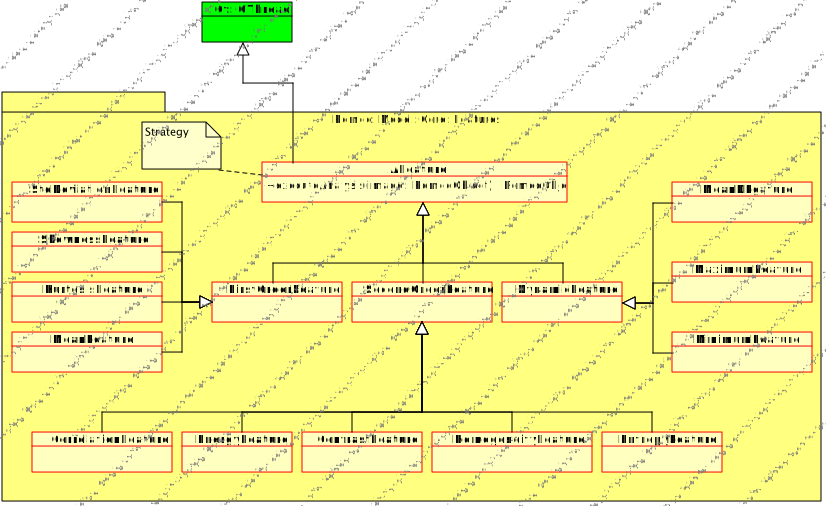
\includegraphics[scale=0.6]{../Specifica_Tecnica/Content/Immagini/Romeo__Model__Core__Adapters__Features.png}
			\caption{Diagramma package \textsl{Romeo::Model::Core::Feature}}
			\label{romeo_model_core}
\end{figure}

Package\g{} contenente le classi per le feature\g{}.

% % % % % % % % % % % % % % % % % % % % % %
% % % % % % % % % % % % % % % % % % % %
\subsubsection{AFeature (abstract)}
\label{afeature}
\begin{figure}[!h]
\centering
			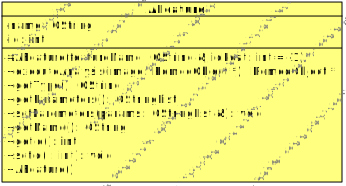
\includegraphics[scale=1]{./Content/Immagini/modelCore/AFeature.png}
			\caption{Diagramma classe \textsl{AFeature}}
			\label{feature_img}
\end{figure}

\paragraph{Descrizione \\} Classe astratta che rappresenta una generica feature\g{}. Definisce dei contratti per l'esecuzione degli algoritmi, che dovranno essere implementati dalle sue sottoclassi. Rappresenta la componente Strategy dell'omonimo design pattern\g{}.

\paragraph{Utilizzo\\} Fornisce i metodi per l'esecuzione di una feature\g{} su un immagine bidimensionale o tridimensionale.

\paragraph{Eredita da}
\begin{itemize}
	\item Qt::QThread
\end{itemize}

\paragraph{\textcolor{black}{Attributi\\}}
	\begin{itemize}
		\item \color{teal}\verb!- name : QString !
		\color{black}
		\subparagraph{Descrizione:} stringa contenente il nome della feature\g{}.
		\item \color{teal}\verb!- id : int !
		\color{black}
		\subparagraph{Descrizione:} intero contentente il codice identificativo della feature\g{}.
	\end{itemize}

\paragraph{\textcolor{black}{Metodi\\}}
	\begin{itemize}
	\item \color{blue}\verb! # AFeature(featureName : const QString & , id :	int)!
		\color{black}
		\subparagraph{Descrizione:} costruttore della classe AFeature.
		\subparagraph{Argomenti}
			\begin{itemize}
				\item \color{RoyalPurple} \verb!name : const QString &! \\ 
				\color{black} nome della feature\g{}.	
				\item \color{RoyalPurple} \verb!id : int! \\ 
				\color{black} codice identificativo della feature\g{}.	
			\end{itemize}
			
	\item \color{blue}\verb! + executeAnalysis(image : RomeoObject *) : RomeoObject *!
		\color{black}
		\subparagraph{Descrizione:} metodo puro che esegue la feature su un dato e ritorna il dato di output.
		\subparagraph{Argomenti}
			\begin{itemize}
				\item \color{RoyalPurple} \verb!image : RomeoObject * ! \\ 
				\color{black} dato in ingresso alla feature.		
			\end{itemize}
		\subparagraph{Note}
			\begin{itemize}
				\item il metodo deve essere marcato virtuale puro.
			\end{itemize}
			
	\item \color{blue}\verb! + getType() : QString !
		\color{black}
		\subparagraph{Descrizione:}  contratto per restituire il tipo della feature\g{}.
		\subparagraph{Note}
			\begin{itemize}
				\item deve essere marcato costante.
			\end{itemize}
			
	\item \color{blue}\verb! + getParameters() : QStringList!
		\color{black}
		\subparagraph{Descrizione:}  contratto per restituisce una lista di stringe, contenente la lista degli 						attributi.
		\subparagraph{Note}
			\begin{itemize}
				\item deve essere marcato costante.
			\end{itemize}
	
	\item \color{blue}\verb! + setParameters(params : const QStringList &) : void !
		\color{black}
		\subparagraph{Descrizione:} inserisce i parametri della feature\g{}.
		\subparagraph{Argomenti}
			\begin{itemize}
				\item \color{RoyalPurple} \verb!params : const QStringList & ! \\ 
				\color{black} lista di parametri della feature.		
			\end{itemize}
		\subparagraph{Note}
			\begin{itemize}
				\item il metodo deve essere marcato virtuale.
			\end{itemize}
		
	\item \color{blue}\verb! + getName() : QString!
		\color{black}
		\subparagraph{Descrizione:} restituisce il nome della feature\g{}.
		\subparagraph{Note}
			\begin{itemize}
				\item deve essere marcato costante.
			\end{itemize}
			
	\item \color{blue}\verb! + getId() : int!
		\color{black}
		\subparagraph{Descrizione:} restituisce il codice identificativo della feature\g{}.
		\subparagraph{Note}
			\begin{itemize}
				\item deve essere marcato costante.
			\end{itemize}
			
	\item \color{blue}\verb! + setId(i : int) : void!
		\color{black}
		\subparagraph{Descrizione:} inserisce il codice identificativo della feature.
		\subparagraph{Argomenti}
			\begin{itemize}
				\item \color{RoyalPurple} \verb!params : const QStringList & ! \\ 
				\color{black} codice identificativo della feature.		
			\end{itemize}

	\end{itemize}
	

% % % % % % % % % % % % % % % % % % % % % % % % % % % % % % % % %
% % % % % % FIRST ORDER FEATURE % % % % % % % % % % % % % % % % % % % % % %
% % % % % % % % % % % % % % % % % % % % % % % % % % % % % %
\color{black}
\pagebreak
\subsubsection{FirstOrderFeature (abstract)}
\label{FirstOrderFeature}
\begin{figure}[!h]
\centering
			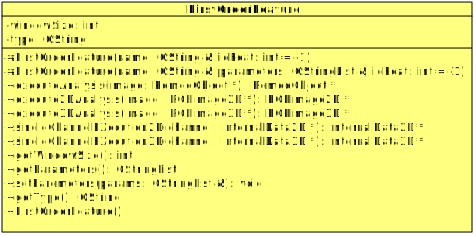
\includegraphics[scale=1]{./Content/Immagini/modelCore/FirstOrderFeature.png}
			\caption{Diagramma classe \textsl{FirstOrderFeature}}
			\label{FirstOrderFeature_img}
\end{figure}

\paragraph{Descrizione \\} Classe astratta che rappresenta una generica feature\g{} del primo ordine. Deriva da AFeature e rimane astratta perché non implementa i contratti di quest'ultima. Le sue sottoclassi rappresenteranno le componenti ConcreteStrategy del design pattern\g{} Strategy.

\paragraph{Utilizzo\\} Viene utilizzata durante un'analisi recuperare le informazioni sulla dimensione della finestra, la lista dei parametri e il tipo della feature\g{}.

\paragraph{Eredita da:}
\begin{itemize}
	\item AFeature.
\end{itemize}

\paragraph{\textcolor{black}{Attributi\\}}
	\begin{itemize}
		\item \color{teal}\verb!- windowSize : int!
		\color{black}
		\subparagraph{Descrizione:} dimensione della finestra sulla quale effettuare le operazioni.
		\item \color{teal}\verb!- type : QString!
		\color{black}
		\subparagraph{Descrizione:} specifica il tipo della feature\g{}.
	\end{itemize}

\paragraph{\textcolor{black}{Metodi\\}}
	\begin{itemize}
	\item \color{blue}\verb! # FirstOrderFeature(name : QString & , idFeat : int)!
		\color{black}
		\subparagraph{Descrizione:} costruttore della classe FirstOrderFeature.
		\subparagraph{Argomenti}
			\begin{itemize}
				\item \color{RoyalPurple} \verb!name : QString &! \\ 
				\color{black} Nome della feature. Viene passato al costruttore della superclasse.	
				\item \color{RoyalPurple} \verb!id : int! \\ 
				\color{black} codice identificativo della feature\g{}.	
			\end{itemize}
			
	\item \color{blue}\verb! # FirstOrderFeature(name : QString &, parameters : QStringList & , id : int)!
		\color{black}
		\subparagraph{Descrizione:} Costruttore a tre parametri della classe. Richiama il costruttore della 						superclasse.
		\subparagraph{Argomenti}
			\begin{itemize}
				\item \color{RoyalPurple} \verb!name : QString &! \\ 
				\color{black} Nome della feature. Viene passato al costruttore della superclasse.	
				\item \color{RoyalPurple} \verb!parameters : QStringList &! \\ 
				\color{black} Lista contenente i parametri della feature\g{}. Verrà effettuato il \textit{parsing} 						della lista, dalla quale verrà estratta la dimensione della finestra.
				\item \color{RoyalPurple} \verb!id : int! \\ 
				\color{black} codice identificativo della feature\g{}.	
			\end{itemize}
			
	\item \color{blue}\verb! + executeAnalysis(image : RomeoObject *) : RomeoObject *!
		\color{black}
		\subparagraph{Descrizione:} metodo puro che esegue la feature su un dato e ritorna il dato di output.
		\subparagraph{Argomenti}
			\begin{itemize}
				\item \color{RoyalPurple} \verb!image : RomeoObject * ! \\ 
				\color{black} dato in ingresso alla feature.		
			\end{itemize}
		\subparagraph{Note}
			\begin{itemize}
				\item il metodo deve essere marcato virtuale.
			\end{itemize}
						
	\item \color{blue}\verb! + execute2DAnalysis(image : RGBImage2D *) : RGBImage2D *!
		\color{black}
		\subparagraph{Descrizione:} metodo puro che esegue la feature su un immagine 2D e ritorna un immagine 2D 						processata.
		\subparagraph{Argomenti}
			\begin{itemize}
				\item \color{RoyalPurple} \verb!image : RGBImage2D * ! \\ 
				\color{black} immagine 2D in ingresso alla feature.		
			\end{itemize}
		\subparagraph{Note}
			\begin{itemize}
				\item il metodo deve essere marcato virtuale.
			\end{itemize}
			
	\item \color{blue}\verb! + execute3DAnalysis(image : RGBImage3D *) : RGBImage3D *!
		\color{black}
		\subparagraph{Descrizione:} metodo puro che esegue la feature su un immagine 3D e ritorna un immagine 3D 						processata.
		\subparagraph{Argomenti}
			\begin{itemize}
				\item \color{RoyalPurple} \verb!image : RGBImage3D * ! \\ 
				\color{black} immagine 3D in ingresso alla feature.		
			\end{itemize}
		\subparagraph{Note}
			\begin{itemize}
				\item il metodo deve essere marcato virtuale.
			\end{itemize}
			
	\item \color{blue}\verb! + singleChannelEXecution2D(channel : InternalData2D *) : InternalData2D *!
		\color{black}
		\subparagraph{Descrizione:} metodo puro che esegue la feature su un canale di un immagine 2D.
		\subparagraph{Argomenti}
			\begin{itemize}
				\item \color{RoyalPurple} \verb!channel : InternalData2D * ! \\ 
				\color{black} canale di un immagine 2D in ingresso alla feature.		
			\end{itemize}
		\subparagraph{Note}
			\begin{itemize}
				\item il metodo deve essere marcato virtuale puro.
			\end{itemize}
			
	\item \color{blue}\verb! + singleChannelEXecution3D(channel : InternalData3D *) : InternalData3D *!
		\color{black}
		\subparagraph{Descrizione:} metodo puro che esegue la feature su un canale di un immagine 3D.
		\subparagraph{Argomenti}
			\begin{itemize}
				\item \color{RoyalPurple} \verb!channel : InternalData3D * ! \\ 
				\color{black} canale di un immagine 3D in ingresso alla feature.		
			\end{itemize}
		\subparagraph{Note}
			\begin{itemize}
				\item il metodo deve essere marcato virtuale puro.
			\end{itemize}
			
	\item \color{blue}\verb! + getWindowSize() : int!
		\color{black}
		\subparagraph{Descrizione:} metodo che ritorna la dimensione della finestra .
		\subparagraph{Note}
			\begin{itemize}
				\item il metodo deve essere marcato costante.
			\end{itemize}
			
	\item \color{blue}\verb! + getParameters() : QStringList!
		\color{black}
		\subparagraph{Descrizione:} metodo che ritorna la lista dei parametri della feature\g{} .
		\subparagraph{Note}
			\begin{itemize}
				\item il metodo deve essere marcato virtuale.
			\end{itemize}
			
	\item \color{blue}\verb! + setParameters(params : const QStringList &) : void!
		\color{black}
		\subparagraph{Descrizione:} inserisce i parametri della feature\g{}.
		\subparagraph{Argomenti}
			\begin{itemize}
				\item \color{RoyalPurple} \verb!params : const QStringList & ! \\ 
				\color{black} lista di parametri della feature.		
			\end{itemize}
		\subparagraph{Note}
			\begin{itemize}
				\item il metodo deve essere marcato virtuale.
			\end{itemize}
			
	\item \color{blue}\verb! + getType() : QString!
		\color{black}
		\subparagraph{Descrizione:} metodo che ritorna il tipo della feature\g{} .
		\subparagraph{Note}
			\begin{itemize}
				\item il metodo deve essere marcato costante.
				\item il metodo deve essere marcato virtuale.
			\end{itemize}
			
	\end{itemize}


% % % % % % % % % % % % % % % % % % % % % % % % % % % % % % % % %
% % % % % % SECOND ORDER FEATURE% % % % % % % % % % % % % % % % % % % % % % %
% % % % % % % % % % % % % % % % % % % % % % % % % % % % % %
\color{black}
\pagebreak
\subsubsection{SecondOrderFeature (abstract)}
\label{SecondOrderFeature}
\begin{figure}[!h]
\centering
			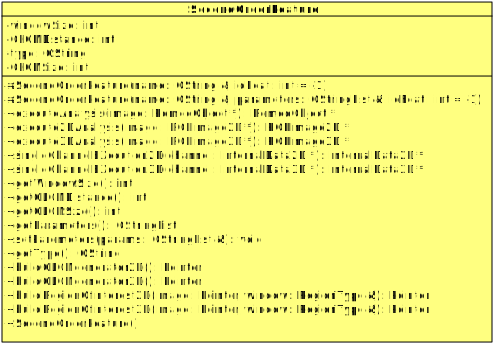
\includegraphics[scale=1]{./Content/Immagini/modelCore/SecondOrderFeature.png}
			\caption{Diagramma classe \textsl{SecondOrderFeature}}
			\label{SecondOrder_img}
\end{figure}

\paragraph{Descrizione \\} Classe astratta che rappresenta una generica feature\g{} del secondo ordine. Deriva da AFeature e rimane astratta perché non implementa i contratti di quest'ultima. Le sue sottoclassi rappresenteranno le componenti ConcreteStrategy del design pattern\g{} Strategy.

\paragraph{Utilizzo\\} Viene utilizzata durante un'analisi recuperare le informazioni della feature\g{}, la lista dei parametri e il tipo della feature\g{}.

\paragraph{Eredita da:}
\begin{itemize}
	\item AFeature.
\end{itemize}

\paragraph{\textcolor{black}{Attributi\\}}
	\begin{itemize}
		\item \color{teal}\verb!- windowSize : int!
		\color{black}
		\subparagraph{Descrizione:} dimensione della finestra sulla quale effettuare le operazioni.
		\item \color{teal}\verb!- type : QString!
		\color{black}
		\subparagraph{Descrizione:} specifica il tipo della feature\g{}.
		\item \color{teal}\verb!- GLCMSize : int!
		\color{black}
		\subparagraph{Descrizione:} specifica la dimensione della matrice GLCM.
		\item \color{teal}\verb!- GLCMDistance : int!
		\color{black}
		\subparagraph{Descrizione:} specifica la distanza della matrice GLCM.
	\end{itemize}

\paragraph{\textcolor{black}{Metodi\\}}
	\begin{itemize}
	\item \color{blue}\verb! # SecondOrderFeature(name : QString & , idFeat : int)!
		\color{black}
		\subparagraph{Descrizione:} costruttore della classe SecondOrderFeature.
		\subparagraph{Argomenti}
			\begin{itemize}
				\item \color{RoyalPurple} \verb!name : QString &! \\ 
				\color{black} Nome della feature. Viene passato al costruttore della superclasse.	
				\item \color{RoyalPurple} \verb!id : int! \\ 
				\color{black} codice identificativo della feature\g{}.	
			\end{itemize}
			
	\item \color{blue}\verb! # SecondOrderFeature(name : QString &, parameters : QStringList & , id : int)!
		\color{black}
		\subparagraph{Descrizione:} Costruttore a tre parametri della classe. Richiama il costruttore della 						superclasse.
		\subparagraph{Argomenti}
			\begin{itemize}
				\item \color{RoyalPurple} \verb!name : QString &! \\ 
				\color{black} Nome della feature. Viene passato al costruttore della superclasse.	
				\item \color{RoyalPurple} \verb!parameters : QStringList &! \\ 
				\color{black} Lista contenente i parametri della feature\g{}. Verrà effettuato il \textit{parsing} 						della lista, dalla quale verrà estratta la dimensione della finestra.
				\item \color{RoyalPurple} \verb!id : int! \\ 
				\color{black} codice identificativo della feature\g{}.	
			\end{itemize}
			
	\item \color{blue}\verb! + executeAnalysis(image : RomeoObject *) : RomeoObject *!
		\color{black}
		\subparagraph{Descrizione:} metodo puro che esegue la feature su un dato e ritorna il dato di output.
		\subparagraph{Argomenti}
			\begin{itemize}
				\item \color{RoyalPurple} \verb!image : RomeoObject * ! \\ 
				\color{black} dato in ingresso alla feature.		
			\end{itemize}
		\subparagraph{Note}
			\begin{itemize}
				\item il metodo deve essere marcato virtuale.
			\end{itemize}
						
	\item \color{blue}\verb! + execute2DAnalysis(image : RGBImage2D *) : RGBImage2D *!
		\color{black}
		\subparagraph{Descrizione:} metodo puro che esegue la feature su un immagine 2D e ritorna un immagine 2D 						processata.
		\subparagraph{Argomenti}
			\begin{itemize}
				\item \color{RoyalPurple} \verb!image : RGBImage2D * ! \\ 
				\color{black} immagine 2D in ingresso alla feature.		
			\end{itemize}
		\subparagraph{Note}
			\begin{itemize}
				\item il metodo deve essere marcato virtuale.
			\end{itemize}
			
	\item \color{blue}\verb! + execute3DAnalysis(image : RGBImage3D *) : RGBImage3D *!
		\color{black}
		\subparagraph{Descrizione:} metodo puro che esegue la feature su un immagine 3D e ritorna un immagine 3D 						processata.
		\subparagraph{Argomenti}
			\begin{itemize}
				\item \color{RoyalPurple} \verb!image : RGBImage3D * ! \\ 
				\color{black} immagine 3D in ingresso alla feature.		
			\end{itemize}
		\subparagraph{Note}
			\begin{itemize}
				\item il metodo deve essere marcato virtuale.
			\end{itemize}
			
	\item \color{blue}\verb! + singleChannelEXecution2D(channel : InternalData2D *) : InternalData2D *!
		\color{black}
		\subparagraph{Descrizione:} metodo puro che esegue la feature su un canale di un immagine 2D.
		\subparagraph{Argomenti}
			\begin{itemize}
				\item \color{RoyalPurple} \verb!channel : InternalData2D * ! \\ 
				\color{black} canale di un immagine 2D in ingresso alla feature.		
			\end{itemize}
		\subparagraph{Note}
			\begin{itemize}
				\item il metodo deve essere marcato virtuale puro.
			\end{itemize}
			
	\item \color{blue}\verb! + singleChannelEXecution3D(channel : InternalData3D *) : InternalData3D *!
		\color{black}
		\subparagraph{Descrizione:} metodo puro che esegue la feature su un canale di un immagine 3D.
		\subparagraph{Argomenti}
			\begin{itemize}
				\item \color{RoyalPurple} \verb!channel : InternalData3D * ! \\ 
				\color{black} canale di un immagine 3D in ingresso alla feature.		
			\end{itemize}
		\subparagraph{Note}
			\begin{itemize}
				\item il metodo deve essere marcato virtuale puro.
			\end{itemize}
			
	\item \color{blue}\verb! + getWindowSize() : int!
		\color{black}
		\subparagraph{Descrizione:} metodo che ritorna la dimensione della finestra .
		\subparagraph{Note}
			\begin{itemize}
				\item il metodo deve essere marcato costante.
			\end{itemize}
			
	\item \color{blue}\verb! + getGLCMDistance() : int!
		\color{black}
		\subparagraph{Descrizione:} metodo che ritorna la distanza della matrice GLCM	.
		\subparagraph{Note}
			\begin{itemize}
				\item il metodo deve essere marcato costante.
			\end{itemize}
			
	\item \color{blue}\verb! + getGLCMSize() : int!
		\color{black}
		\subparagraph{Descrizione:} metodo che ritorna la dimensione della matrice GLCM	.
		\subparagraph{Note}
			\begin{itemize}
				\item il metodo deve essere marcato costante.
			\end{itemize}
			
			
	\item \color{blue}\verb! + getParameters() : QStringList!
		\color{black}
		\subparagraph{Descrizione:} metodo che ritorna la lista dei parametri della feature\g{} .
		\subparagraph{Note}
			\begin{itemize}
				\item il metodo deve essere marcato virtuale.
			\end{itemize}
			
	\item \color{blue}\verb! + setParameters(params : const QStringList &) : void!
		\color{black}
		\subparagraph{Descrizione:} inserisce i parametri della feature\g{}.
		\subparagraph{Argomenti}
			\begin{itemize}
				\item \color{RoyalPurple} \verb!params : const QStringList & ! \\ 
				\color{black} lista di parametri della feature.		
			\end{itemize}
		\subparagraph{Note}
			\begin{itemize}
				\item il metodo deve essere marcato virtuale.
			\end{itemize}
			
	\item \color{blue}\verb! + getType() : QString!
		\color{black}
		\subparagraph{Descrizione:} metodo che ritorna il tipo della feature\g{} .
		\subparagraph{Note}
			\begin{itemize}
				\item il metodo deve essere marcato costante.
				\item il metodo deve essere marcato virtuale.
			\end{itemize}
			
			
	\item \color{blue}\verb! + buildGLCMgenerator2D() : InternalData2D::ImageToGlcmType::Pointer !
		\color{black}
		\subparagraph{Descrizione:} costruisce l'oggetto che si occupa del calcolo della GLCM per le immagini 2D.
		
	\item \color{blue}\verb! + buildGLCMgenerator3D() : InternalData3D::ImageToGlcmType::Pointer !
		\color{black}
		\subparagraph{Descrizione:} costruisce l'oggetto che si occupa del calcolo della GLCM per le immagini 3D.
		
	\item \color{blue}\verb! + buildRegionOfInterest2D(image : InternalData2D::ImageType::Pointer , !\\																	\verb!window : InternalData2D::ImageType::RegionType &) !\\
													\verb!: InternalData2D::roiType::Pointer  !					
		\color{black}
		\subparagraph{Descrizione:} costruisce la regione di iterazione per le immagini 2D.
		\subparagraph{Argomenti}
			\begin{itemize}
				\item \color{RoyalPurple} \verb!image : InternalData2D::ImageType::Pointer ! \\ 
				\color{black} immagine in input.		
			\end{itemize}
			\begin{itemize}
				\item \color{RoyalPurple} \verb!window : InternalData2D::ImageType::RegionType & ! \\ 
				\color{black} regione dell'immagine da scorrere.		
			\end{itemize}
			
	\item \color{blue}\verb! + buildRegionOfInterest3D(image : InternalData3D::ImageType::Pointer , !\\																	\verb!window : InternalData3D::ImageType::RegionType &) !\\
													\verb!: InternalData3D::roiType::Pointer  !					
		\color{black}
		\subparagraph{Descrizione:} costruisce la regione di iterazione per le immagini 3D.
		\subparagraph{Argomenti}
			\begin{itemize}
				\item \color{RoyalPurple} \verb!image : InternalData3D::ImageType::Pointer ! \\ 
				\color{black} immagine in input.		
			\end{itemize}
			\begin{itemize}
				\item \color{RoyalPurple} \verb!window : InternalData3D::ImageType::RegionType & ! \\ 
				\color{black} regione dell'immagine da scorrere.		
			\end{itemize}
		
	\end{itemize}

% % % % % % % % % % % % % % % % % % % % % % % % % % % % % % % % %
% % % % % % DYNAMIC FEATURE% % % % % % % % % % % % % % % % % % % % % % %
% % % % % % % % % % % % % % % % % % % % % % % % % % % % % %
\color{black}
\pagebreak
\subsubsection{DynamicFeature (abstract)}
\label{DynamicFeature}
\begin{figure}[!h]
\centering
			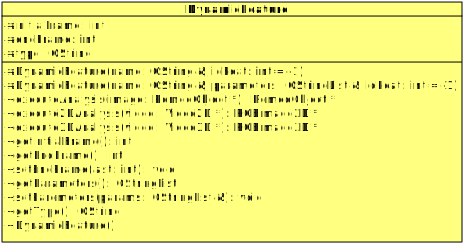
\includegraphics[scale=1]{./Content/Immagini/modelCore/DynamicFeature.png}
			\caption{Diagramma classe \textsl{DynamicFeature}}
			\label{Dynamic_img}
\end{figure}

\paragraph{Descrizione \\} Classe astratta che rappresenta una generica feature\g{} dinamica. Deriva da AFeature e rimane astratta perché non implementa i contratti di quest'ultima. Le sue sottoclassi rappresenteranno le componenti ConcreteStrategy del design pattern\g{} Strategy.

\paragraph{Utilizzo\\} Viene utilizzata durante un'analisi recuperare la lista dei parametri e il tipo della feature\g{}.

\paragraph{Eredita da:}
\begin{itemize}
	\item AFeature.
\end{itemize}

\paragraph{\textcolor{black}{Attributi\\}}
	\begin{itemize}
		\item \color{teal}\verb!- type : QString!
		\color{black}
		\subparagraph{Descrizione:} specifica il tipo della feature\g{}.
		\item \color{teal}\verb!- initialFrame : int!
		\color{black}
		\subparagraph{Descrizione:} specifica il frame d'inizio del video.
		\item \color{teal}\verb!- endFrame : int!
		\color{black}
		\subparagraph{Descrizione:} specifica l'ultimo frame del video.
	\end{itemize}

\paragraph{\textcolor{black}{Metodi\\}}
	\begin{itemize}
	\item \color{blue}\verb! # DynamicFeature(name : QString & , idFeat : int)!
		\color{black}
		\subparagraph{Descrizione:} costruttore della classe SecondOrderFeature.
		\subparagraph{Argomenti}
			\begin{itemize}
				\item \color{RoyalPurple} \verb!name : QString &! \\ 
				\color{black} Nome della feature. Viene passato al costruttore della superclasse.	
				\item \color{RoyalPurple} \verb!id : int! \\ 
				\color{black} codice identificativo della feature\g{}.	
			\end{itemize}
			
	\item \color{blue}\verb! # DynamicFeature(name : QString &, parameters : QStringList & , id : int)!
		\color{black}
		\subparagraph{Descrizione:} Costruttore a tre parametri della classe. Richiama il costruttore della 						superclasse.
		\subparagraph{Argomenti}
			\begin{itemize}
				\item \color{RoyalPurple} \verb!name : QString &! \\ 
				\color{black} Nome della feature. Viene passato al costruttore della superclasse.	
				\item \color{RoyalPurple} \verb!parameters : QStringList &! \\ 
				\color{black} Lista contenente i parametri della feature\g{}. Verrà effettuato il \textit{parsing} 						della lista, dalla quale verrà estratta la dimensione della finestra.
				\item \color{RoyalPurple} \verb!id : int! \\ 
				\color{black} codice identificativo della feature\g{}.	
			\end{itemize}
			
	\item \color{blue}\verb! + executeAnalysis(image : RomeoObject *) : RomeoObject *!
		\color{black}
		\subparagraph{Descrizione:} metodo puro che esegue la feature su un dato e ritorna il dato di output.
		\subparagraph{Argomenti}
			\begin{itemize}
				\item \color{RoyalPurple} \verb!image : RomeoObject * ! \\ 
				\color{black} dato in ingresso alla feature.		
			\end{itemize}
		\subparagraph{Note}
			\begin{itemize}
				\item il metodo deve essere marcato virtuale.
			\end{itemize}
						
	\item \color{blue}\verb! + execute2DAnalysis(image : RGBImage2D *) : RGBImage2D *!
		\color{black}
		\subparagraph{Descrizione:} metodo puro che esegue la feature su un immagine 2D e ritorna un immagine 2D 						processata.
		\subparagraph{Argomenti}
			\begin{itemize}
				\item \color{RoyalPurple} \verb!image : RGBImage2D * ! \\ 
				\color{black} immagine 2D in ingresso alla feature.		
			\end{itemize}
		\subparagraph{Note}
			\begin{itemize}
				\item il metodo deve essere marcato virtuale.
			\end{itemize}
			
	\item \color{blue}\verb! + execute3DAnalysis(image : RGBImage3D *) : RGBImage3D *!
		\color{black}
		\subparagraph{Descrizione:} metodo puro che esegue la feature su un immagine 3D e ritorna un immagine 3D 						processata.
		\subparagraph{Argomenti}
			\begin{itemize}
				\item \color{RoyalPurple} \verb!image : RGBImage3D * ! \\ 
				\color{black} immagine 3D in ingresso alla feature.		
			\end{itemize}
		\subparagraph{Note}
			\begin{itemize}
				\item il metodo deve essere marcato virtuale.
			\end{itemize}
			
	\item \color{blue}\verb! + getInitialFrame() : int!
		\color{black}
		\subparagraph{Descrizione:} metodo che ritorna l'indice del frame iniziale.
		\subparagraph{Note}
			\begin{itemize}
				\item il metodo deve essere marcato costante.
			\end{itemize}
			
	\item \color{blue}\verb! + getEndFrame() : int!
		\color{black}
		\subparagraph{Descrizione:} metodo che ritorna il frame finale.
		\subparagraph{Note}
			\begin{itemize}
				\item il metodo deve essere marcato costante.
			\end{itemize}
	
	\item \color{blue}\verb! + setEndFrame(last : int) : void!
		\color{black}
		\subparagraph{Descrizione:} metodo che inserisce l'indice dell'ultimo frame del video da considerare.
		\subparagraph{Argomenti}
			\begin{itemize}
				\item \color{RoyalPurple} \verb!last : int! \\ 
				\color{black} indice dell'ultimo frame del video da considerare.		
			\end{itemize}		
						
	\item \color{blue}\verb! + getParameters() : QStringList!
		\color{black}
		\subparagraph{Descrizione:} metodo che ritorna la lista dei parametri della feature\g{} .
		\subparagraph{Note}
			\begin{itemize}
				\item il metodo deve essere marcato virtuale.
			\end{itemize}
			
	\item \color{blue}\verb! + setParameters(params : const QStringList &) : void!
		\color{black}
		\subparagraph{Descrizione:} inserisce i parametri della feature\g{}.
		\subparagraph{Argomenti}
			\begin{itemize}
				\item \color{RoyalPurple} \verb!params : const QStringList & ! \\ 
				\color{black} lista di parametri della feature.		
			\end{itemize}
		\subparagraph{Note}
			\begin{itemize}
				\item il metodo deve essere marcato virtuale.
			\end{itemize}
			
	\item \color{blue}\verb! + getType() : QString!
		\color{black}
		\subparagraph{Descrizione:} metodo che ritorna il tipo della feature\g{} .
		\subparagraph{Note}
			\begin{itemize}
				\item il metodo deve essere marcato costante.
				\item il metodo deve essere marcato virtuale.
			\end{itemize}
		
	\end{itemize}


% % % % % % % % % % % % % % % % % % % % % % % % % % % % % % % % %
% % % % % % MEAN FEATURE % % % % % % % % % % % % % % % % % % % % % % %
% % % % % % % % % % % % % % % % % % % % % % % % % % % % % %
\color{black}
\pagebreak
\subsubsection{MeanFeature (class)}
\label{MeanFeature}
\begin{figure}[!h]
\centering
			\includegraphics[scale=1]{./Content/Immagini/modelCore/MeanFeature.png}
			\caption{Diagramma classe \textsl{MeanFeature}}
			\label{meanFeature_img}
\end{figure}

\paragraph{Descrizione \\} Classe che implementa la feature\g{} \textit{Mean}. Rappresenta la componente ConcreteStrategy del design pattern\g{} Strategy.
\\Per l'implementazione della feature\g{} il programmatore dovrà seguire l'appendice \ref{codicematlab}.

\paragraph{Utilizzo\\} Viene utilizzata durante un'analisi per applicare la feature\g{} a un \dataset{}.

\paragraph{Eredita da:}
\begin{itemize}
	\item FirstOrderFeature.
\end{itemize}

\paragraph{\textcolor{black}{Metodi\\}}
	\begin{itemize}
	\item \color{blue}\verb! # DynamicFeature(idFeat : int)!
		\color{black}
		\subparagraph{Descrizione:} costruttore della classe MeanFeature.
		\subparagraph{Argomenti}
			\begin{itemize}
				\item \color{RoyalPurple} \verb!id : int! \\ 
				\color{black} codice identificativo della feature\g{}.	
			\end{itemize}
			
	\item \color{blue}\verb! # DynamicFeature(parameters : QStringList & , id : int)!
		\color{black}
		\subparagraph{Descrizione:} Costruttore a due parametri della classe. Richiama il costruttore della 						superclasse.
		\subparagraph{Argomenti}
			\begin{itemize}	
				\item \color{RoyalPurple} \verb!parameters : QStringList &! \\ 
				\color{black} Lista contenente i parametri della feature\g{}. Verrà effettuato il \textit{parsing} 						della lista, dalla quale verrà estratta la dimensione della finestra.
				\item \color{RoyalPurple} \verb!id : int! \\ 
				\color{black} codice identificativo della feature\g{}.	
			\end{itemize}

	\item \color{blue}\verb! + singleChannelEXecution2D(channel : InternalData2D *) : InternalData2D *!
		\color{black}
		\subparagraph{Descrizione:} metodo puro che esegue la feature su un canale di un immagine 2D.
		\subparagraph{Argomenti}
			\begin{itemize}
				\item \color{RoyalPurple} \verb!channel : InternalData2D * ! \\ 
				\color{black} canale di un immagine 2D in ingresso alla feature.		
			\end{itemize}
		\subparagraph{Note}
			\begin{itemize}
				\item il metodo deve essere marcato virtuale puro.
			\end{itemize}
			
	\item \color{blue}\verb! + singleChannelEXecution3D(channel : InternalData3D *) : InternalData3D *!
		\color{black}
		\subparagraph{Descrizione:} metodo puro che esegue la feature su un canale di un immagine 3D.
		\subparagraph{Argomenti}
			\begin{itemize}
				\item \color{RoyalPurple} \verb!channel : InternalData3D * ! \\ 
				\color{black} canale di un immagine 3D in ingresso alla feature.		
			\end{itemize}
		\subparagraph{Note}
			\begin{itemize}
				\item il metodo deve essere marcato virtuale puro.
			\end{itemize}
			
	\end{itemize}



% % % % % % % % % % % % % % % % % % % % % % % % % % % % % % % % %
% % % % % % KURTOSIS FEATURE % % % % % % % % % % % % % % % % % % % % % % %
% % % % % % % % % % % % % % % % % % % % % % % % % % % % % %
\color{black}
\pagebreak
\subsubsection{KurtosisFeature (class)}
\label{KurtosisFeature}
\begin{figure}[!h]
\centering
			\includegraphics[scale=1]{./Content/Immagini/modelCore/KurtosisFeature.png}
			\caption{Diagramma classe \textsl{KurtosisFeature}}
			\label{kurtosisFeature_img}
\end{figure}

\paragraph{Descrizione \\} Classe che implementa la feature\g{} \textit{Kurtosis}. Rappresenta la componente ConcreteStrategy del design pattern\g{} Strategy.
\\Per l'implementazione della feature\g{} il programmatore dovrà seguire l'appendice \ref{codicematlab}.

\paragraph{Utilizzo\\} Viene utilizzata durante un'analisi per applicare la feature\g{} a un \dataset{}.

\paragraph{Eredita da:}
\begin{itemize}
	\item FirstOrderFeature.
\end{itemize}

\paragraph{\textcolor{black}{Metodi\\}}
	\begin{itemize}
	\item \color{blue}\verb! # DynamicFeature(idFeat : int)!
		\color{black}
		\subparagraph{Descrizione:} costruttore della classe MeanFeature.
		\subparagraph{Argomenti}
			\begin{itemize}
				\item \color{RoyalPurple} \verb!id : int! \\ 
				\color{black} codice identificativo della feature\g{}.	
			\end{itemize}
			
	\item \color{blue}\verb! # DynamicFeature(parameters : QStringList & , id : int)!
		\color{black}
		\subparagraph{Descrizione:} Costruttore a due parametri della classe. Richiama il costruttore della 						superclasse.
		\subparagraph{Argomenti}
			\begin{itemize}	
				\item \color{RoyalPurple} \verb!parameters : QStringList &! \\ 
				\color{black} Lista contenente i parametri della feature\g{}. Verrà effettuato il \textit{parsing} 						della lista, dalla quale verrà estratta la dimensione della finestra.
				\item \color{RoyalPurple} \verb!id : int! \\ 
				\color{black} codice identificativo della feature\g{}.	
			\end{itemize}

	\item \color{blue}\verb! + singleChannelEXecution2D(channel : InternalData2D *) : InternalData2D *!
		\color{black}
		\subparagraph{Descrizione:} metodo puro che esegue la feature su un canale di un immagine 2D.
		\subparagraph{Argomenti}
			\begin{itemize}
				\item \color{RoyalPurple} \verb!channel : InternalData2D * ! \\ 
				\color{black} canale di un immagine 2D in ingresso alla feature.		
			\end{itemize}
		\subparagraph{Note}
			\begin{itemize}
				\item il metodo deve essere marcato virtuale puro.
			\end{itemize}
			
	\item \color{blue}\verb! + singleChannelEXecution3D(channel : InternalData3D *) : InternalData3D *!
		\color{black}
		\subparagraph{Descrizione:} metodo puro che esegue la feature su un canale di un immagine 3D.
		\subparagraph{Argomenti}
			\begin{itemize}
				\item \color{RoyalPurple} \verb!channel : InternalData3D * ! \\ 
				\color{black} canale di un immagine 3D in ingresso alla feature.		
			\end{itemize}
		\subparagraph{Note}
			\begin{itemize}
				\item il metodo deve essere marcato virtuale puro.
			\end{itemize}
			
	\end{itemize}

% % % % % % % % % % % % % % % % % % % % % % % % % % % % % % % % %
% % % % % % SKEWNESS FEATURE % % % % % % % % % % % % % % % % % % % % % % %
% % % % % % % % % % % % % % % % % % % % % % % % % % % % % %
\color{black}
\pagebreak
\subsubsection{SkewnessFeature (class)}
\label{SkewnessFeature}
\begin{figure}[!h]
\centering
			\includegraphics[scale=1]{./Content/Immagini/modelCore/SkewnessFeature.png}
			\caption{Diagramma classe \textsl{SkewnessFeature}}
			\label{skewnessFeature_img}
\end{figure}

\paragraph{Descrizione \\} Classe che implementa la feature\g{} \textit{Skewness}. Rappresenta la componente ConcreteStrategy del design pattern\g{} Strategy.
\\Per l'implementazione della feature\g{} il programmatore dovrà seguire l'appendice \ref{codicematlab}.

\paragraph{Utilizzo\\} Viene utilizzata durante un'analisi per applicare la feature\g{} a un \dataset{}.

\paragraph{Eredita da:}
\begin{itemize}
	\item FirstOrderFeature.
\end{itemize}

\paragraph{\textcolor{black}{Metodi\\}}
	\begin{itemize}
	\item \color{blue}\verb! # DynamicFeature(idFeat : int)!
		\color{black}
		\subparagraph{Descrizione:} costruttore della classe SkewnessFeature.
		\subparagraph{Argomenti}
			\begin{itemize}
				\item \color{RoyalPurple} \verb!id : int! \\ 
				\color{black} codice identificativo della feature\g{}.	
			\end{itemize}
			
	\item \color{blue}\verb! # DynamicFeature(parameters : QStringList & , id : int)!
		\color{black}
		\subparagraph{Descrizione:} Costruttore a due parametri della classe. Richiama il costruttore della 						superclasse.
		\subparagraph{Argomenti}
			\begin{itemize}	
				\item \color{RoyalPurple} \verb!parameters : QStringList &! \\ 
				\color{black} Lista contenente i parametri della feature\g{}. Verrà effettuato il \textit{parsing} 						della lista, dalla quale verrà estratta la dimensione della finestra.
				\item \color{RoyalPurple} \verb!id : int! \\ 
				\color{black} codice identificativo della feature\g{}.	
			\end{itemize}

	\item \color{blue}\verb! + singleChannelEXecution2D(channel : InternalData2D *) : InternalData2D *!
		\color{black}
		\subparagraph{Descrizione:} metodo puro che esegue la feature su un canale di un immagine 2D.
		\subparagraph{Argomenti}
			\begin{itemize}
				\item \color{RoyalPurple} \verb!channel : InternalData2D * ! \\ 
				\color{black} canale di un immagine 2D in ingresso alla feature.		
			\end{itemize}
		\subparagraph{Note}
			\begin{itemize}
				\item il metodo deve essere marcato virtuale puro.
			\end{itemize}
			
	\item \color{blue}\verb! + singleChannelEXecution3D(channel : InternalData3D *) : InternalData3D *!
		\color{black}
		\subparagraph{Descrizione:} metodo puro che esegue la feature su un canale di un immagine 3D.
		\subparagraph{Argomenti}
			\begin{itemize}
				\item \color{RoyalPurple} \verb!channel : InternalData3D * ! \\ 
				\color{black} canale di un immagine 3D in ingresso alla feature.		
			\end{itemize}
		\subparagraph{Note}
			\begin{itemize}
				\item il metodo deve essere marcato virtuale puro.
			\end{itemize}
			
	\end{itemize}

% % % % % % % % % % % % % % % % % % % % % % % % % % % % % % % % %
% % % % % % STANDARD DEVIATION FEATURE % % % % % % % % % % % % % % % % % % % % % % %
% % % % % % % % % % % % % % % % % % % % % % % % % % % % % %
\color{black}
\pagebreak
\subsubsection{StandardDeviationFeature (class)}
\label{StandardDeviationFeature}
\begin{figure}[!h]
\centering
			\includegraphics[scale=1]{./Content/Immagini/modelCore/StandardDeviationFeature.png}
			\caption{Diagramma classe \textsl{StandardDeviationFeature}}
			\label{standardDeviationFeature_img}
\end{figure}

\paragraph{Descrizione \\} Classe che implementa la feature\g{} \textit{Standard Deviation}. Rappresenta la componente ConcreteStrategy del design pattern\g{} Strategy.
\\Per l'implementazione della feature\g{} il programmatore dovrà seguire l'appendice \ref{codicematlab}.

\paragraph{Utilizzo\\} Viene utilizzata durante un'analisi per applicare la feature\g{} a un \dataset{}.

\paragraph{Eredita da:}
\begin{itemize}
	\item FirstOrderFeature.
\end{itemize}


\paragraph{\textcolor{black}{Metodi\\}}
	\begin{itemize}
	\item \color{blue}\verb! # DynamicFeature(idFeat : int)!
		\color{black}
		\subparagraph{Descrizione:} costruttore della classe StandardDeviationFeature.
		\subparagraph{Argomenti}
			\begin{itemize}
				\item \color{RoyalPurple} \verb!id : int! \\ 
				\color{black} codice identificativo della feature\g{}.	
			\end{itemize}
			
	\item \color{blue}\verb! # DynamicFeature(parameters : QStringList & , id : int)!
		\color{black}
		\subparagraph{Descrizione:} Costruttore a due parametri della classe. Richiama il costruttore della 						superclasse.
		\subparagraph{Argomenti}
			\begin{itemize}	
				\item \color{RoyalPurple} \verb!parameters : QStringList &! \\ 
				\color{black} Lista contenente i parametri della feature\g{}. Verrà effettuato il \textit{parsing} 						della lista, dalla quale verrà estratta la dimensione della finestra.
				\item \color{RoyalPurple} \verb!id : int! \\ 
				\color{black} codice identificativo della feature\g{}.	
			\end{itemize}

	\item \color{blue}\verb! + singleChannelEXecution2D(channel : InternalData2D *) : InternalData2D *!
		\color{black}
		\subparagraph{Descrizione:} metodo puro che esegue la feature su un canale di un immagine 2D.
		\subparagraph{Argomenti}
			\begin{itemize}
				\item \color{RoyalPurple} \verb!channel : InternalData2D * ! \\ 
				\color{black} canale di un immagine 2D in ingresso alla feature.		
			\end{itemize}
		\subparagraph{Note}
			\begin{itemize}
				\item il metodo deve essere marcato virtuale puro.
			\end{itemize}
			
	\item \color{blue}\verb! + singleChannelEXecution3D(channel : InternalData3D *) : InternalData3D *!
		\color{black}
		\subparagraph{Descrizione:} metodo puro che esegue la feature su un canale di un immagine 3D.
		\subparagraph{Argomenti}
			\begin{itemize}
				\item \color{RoyalPurple} \verb!channel : InternalData3D * ! \\ 
				\color{black} canale di un immagine 3D in ingresso alla feature.		
			\end{itemize}
		\subparagraph{Note}
			\begin{itemize}
				\item il metodo deve essere marcato virtuale puro.
			\end{itemize}
			
	\end{itemize}

% % % % % % % % % % % % % % % % % % % % % % % % % % % % % % % % %
% % % % % % CONTRAST FEATURE % % % % % % % % % % % % % % % % % % % % % % %
% % % % % % % % % % % % % % % % % % % % % % % % % % % % % %
\color{black}
\pagebreak
\subsubsection{ContrastFeature (class)}
\label{ConstrastFeature}
\begin{figure}[!h]
\centering
			\includegraphics[scale=1]{./Content/Immagini/modelCore/ContrastFeature.png}
			\caption{Diagramma classe \textsl{ContrastFeature}}
			\label{contrastFeature_img}
\end{figure}

\paragraph{Descrizione \\} Classe che implementa la feature\g{} \textit{Contrast}. Rappresenta la componente ConcreteStrategy del design pattern\g{} Strategy.
\\Per l'implementazione della feature\g{} il programmatore dovrà seguire l'appendice \ref{codicematlab}.

\paragraph{Utilizzo\\} Viene utilizzata durante un'analisi per applicare la feature\g{} a un \dataset{}.

\paragraph{Eredita da:}
\begin{itemize}
	\item SecondOrderFeature.
\end{itemize}


\paragraph{\textcolor{black}{Metodi\\}}
	\begin{itemize}
	\item \color{blue}\verb! # DynamicFeature(idFeat : int)!
		\color{black}
		\subparagraph{Descrizione:} costruttore della classe ContrastFeature.
		\subparagraph{Argomenti}
			\begin{itemize}
				\item \color{RoyalPurple} \verb!id : int! \\ 
				\color{black} codice identificativo della feature\g{}.	
			\end{itemize}
			
	\item \color{blue}\verb! # DynamicFeature(parameters : QStringList & , id : int)!
		\color{black}
		\subparagraph{Descrizione:} Costruttore a due parametri della classe. Richiama il costruttore della 						superclasse.
		\subparagraph{Argomenti}
			\begin{itemize}	
				\item \color{RoyalPurple} \verb!parameters : QStringList &! \\ 
				\color{black} Lista contenente i parametri della feature\g{}. Verrà effettuato il \textit{parsing} 						della lista, dalla quale verrà estratta la dimensione della finestra.
				\item \color{RoyalPurple} \verb!id : int! \\ 
				\color{black} codice identificativo della feature\g{}.	
			\end{itemize}

	\item \color{blue}\verb! + singleChannelEXecution2D(channel : InternalData2D *) : InternalData2D *!
		\color{black}
		\subparagraph{Descrizione:} metodo puro che esegue la feature su un canale di un immagine 2D.
		\subparagraph{Argomenti}
			\begin{itemize}
				\item \color{RoyalPurple} \verb!channel : InternalData2D * ! \\ 
				\color{black} canale di un immagine 2D in ingresso alla feature.		
			\end{itemize}
		\subparagraph{Note}
			\begin{itemize}
				\item il metodo deve essere marcato virtuale puro.
			\end{itemize}
			
	\item \color{blue}\verb! + singleChannelEXecution3D(channel : InternalData3D *) : InternalData3D *!
		\color{black}
		\subparagraph{Descrizione:} metodo puro che esegue la feature su un canale di un immagine 3D.
		\subparagraph{Argomenti}
			\begin{itemize}
				\item \color{RoyalPurple} \verb!channel : InternalData3D * ! \\ 
				\color{black} canale di un immagine 3D in ingresso alla feature.		
			\end{itemize}
		\subparagraph{Note}
			\begin{itemize}
				\item il metodo deve essere marcato virtuale puro.
			\end{itemize}
			
	\end{itemize}
	
% % % % % % % % % % % % % % % % % % % % % % % % % % % % % % % % %
% % % % % % Correlation FEATURE % % % % % % % % % % % % % % % % % % % % % % %
% % % % % % % % % % % % % % % % % % % % % % % % % % % % % %
\color{black}
\pagebreak
\subsubsection{CorrelationFeature (class)}
\label{CorrelationFeature}
\begin{figure}[!h]
\centering
			\includegraphics[scale=1]{./Content/Immagini/modelCore/CorrelationFeature.png}
			\caption{Diagramma classe \textsl{CorrelationFeature}}
			\label{correlationFeature_img}
\end{figure}

\paragraph{Descrizione \\} Classe che implementa la feature\g{} \textit{Correlation}. Rappresenta la componente ConcreteStrategy del design pattern\g{} Strategy.
\\Per l'implementazione della feature\g{} il programmatore dovrà seguire l'appendice \ref{codicematlab}.

\paragraph{Utilizzo\\} Viene utilizzata durante un'analisi per applicare la feature\g{} a un \dataset{}.

\paragraph{Eredita da:}
\begin{itemize}
	\item SecondOrderFeature.
\end{itemize}


\paragraph{\textcolor{black}{Metodi\\}}
	\begin{itemize}
	\item \color{blue}\verb! # DynamicFeature(idFeat : int)!
		\color{black}
		\subparagraph{Descrizione:} costruttore della classe CorrelationFeature.
		\subparagraph{Argomenti}
			\begin{itemize}
				\item \color{RoyalPurple} \verb!id : int! \\ 
				\color{black} codice identificativo della feature\g{}.	
			\end{itemize}
			
	\item \color{blue}\verb! # DynamicFeature(parameters : QStringList & , id : int)!
		\color{black}
		\subparagraph{Descrizione:} Costruttore a due parametri della classe. Richiama il costruttore della 						superclasse.
		\subparagraph{Argomenti}
			\begin{itemize}	
				\item \color{RoyalPurple} \verb!parameters : QStringList &! \\ 
				\color{black} Lista contenente i parametri della feature\g{}. Verrà effettuato il \textit{parsing} 						della lista, dalla quale verrà estratta la dimensione della finestra.
				\item \color{RoyalPurple} \verb!id : int! \\ 
				\color{black} codice identificativo della feature\g{}.	
			\end{itemize}

	\item \color{blue}\verb! + singleChannelEXecution2D(channel : InternalData2D *) : InternalData2D *!
		\color{black}
		\subparagraph{Descrizione:} metodo puro che esegue la feature su un canale di un immagine 2D.
		\subparagraph{Argomenti}
			\begin{itemize}
				\item \color{RoyalPurple} \verb!channel : InternalData2D * ! \\ 
				\color{black} canale di un immagine 2D in ingresso alla feature.		
			\end{itemize}
		\subparagraph{Note}
			\begin{itemize}
				\item il metodo deve essere marcato virtuale puro.
			\end{itemize}
			
	\item \color{blue}\verb! + singleChannelEXecution3D(channel : InternalData3D *) : InternalData3D *!
		\color{black}
		\subparagraph{Descrizione:} metodo puro che esegue la feature su un canale di un immagine 3D.
		\subparagraph{Argomenti}
			\begin{itemize}
				\item \color{RoyalPurple} \verb!channel : InternalData3D * ! \\ 
				\color{black} canale di un immagine 3D in ingresso alla feature.		
			\end{itemize}
		\subparagraph{Note}
			\begin{itemize}
				\item il metodo deve essere marcato virtuale puro.
			\end{itemize}
			
	\end{itemize}
	
% % % % % % % % % % % % % % % % % % % % % % % % % % % % % % % % %
% % % % % % ENERGY FEATURE % % % % % % % % % % % % % % % % % % % % % % %
% % % % % % % % % % % % % % % % % % % % % % % % % % % % % %
\color{black}
\pagebreak
\subsubsection{EnergyFeature (class)}
\label{EnergyFeature}
\begin{figure}[!h]
\centering
			\includegraphics[scale=1]{./Content/Immagini/modelCore/EnergyFeature.png}
			\caption{Diagramma classe \textsl{EnergyFeature}}
			\label{EnergyFeature_img}
\end{figure}

\paragraph{Descrizione \\} Classe che implementa la feature\g{} \textit{Energy}. Rappresenta la componente ConcreteStrategy del design pattern\g{} Strategy.
\\Per l'implementazione della feature\g{} il programmatore dovrà seguire l'appendice \ref{codicematlab}.

\paragraph{Utilizzo\\} Viene utilizzata durante un'analisi per applicare la feature\g{} a un \dataset{}.

\paragraph{Eredita da:}
\begin{itemize}
	\item SecondOrderFeature.
\end{itemize}


\paragraph{\textcolor{black}{Metodi\\}}
	\begin{itemize}
	\item \color{blue}\verb! # DynamicFeature(idFeat : int)!
		\color{black}
		\subparagraph{Descrizione:} costruttore della classe EnergyFeature.
		\subparagraph{Argomenti}
			\begin{itemize}
				\item \color{RoyalPurple} \verb!id : int! \\ 
				\color{black} codice identificativo della feature\g{}.	
			\end{itemize}
			
	\item \color{blue}\verb! # DynamicFeature(parameters : QStringList & , id : int)!
		\color{black}
		\subparagraph{Descrizione:} Costruttore a due parametri della classe. Richiama il costruttore della 						superclasse.
		\subparagraph{Argomenti}
			\begin{itemize}	
				\item \color{RoyalPurple} \verb!parameters : QStringList &! \\ 
				\color{black} Lista contenente i parametri della feature\g{}. Verrà effettuato il \textit{parsing} 						della lista, dalla quale verrà estratta la dimensione della finestra.
				\item \color{RoyalPurple} \verb!id : int! \\ 
				\color{black} codice identificativo della feature\g{}.	
			\end{itemize}

	\item \color{blue}\verb! + singleChannelEXecution2D(channel : InternalData2D *) : InternalData2D *!
		\color{black}
		\subparagraph{Descrizione:} metodo puro che esegue la feature su un canale di un immagine 2D.
		\subparagraph{Argomenti}
			\begin{itemize}
				\item \color{RoyalPurple} \verb!channel : InternalData2D * ! \\ 
				\color{black} canale di un immagine 2D in ingresso alla feature.		
			\end{itemize}
		\subparagraph{Note}
			\begin{itemize}
				\item il metodo deve essere marcato virtuale puro.
			\end{itemize}
			
	\item \color{blue}\verb! + singleChannelEXecution3D(channel : InternalData3D *) : InternalData3D *!
		\color{black}
		\subparagraph{Descrizione:} metodo puro che esegue la feature su un canale di un immagine 3D.
		\subparagraph{Argomenti}
			\begin{itemize}
				\item \color{RoyalPurple} \verb!channel : InternalData3D * ! \\ 
				\color{black} canale di un immagine 3D in ingresso alla feature.		
			\end{itemize}
		\subparagraph{Note}
			\begin{itemize}
				\item il metodo deve essere marcato virtuale puro.
			\end{itemize}
			
	\end{itemize}
	
% % % % % % % % % % % % % % % % % % % % % % % % % % % % % % % % %
% % % % % % ENTROPY FEATURE % % % % % % % % % % % % % % % % % % % % % % %
% % % % % % % % % % % % % % % % % % % % % % % % % % % % % %
\color{black}
\pagebreak
\subsubsection{EntropyFeature (class)}
\label{EntropyFeature}
\begin{figure}[!h]
\centering
			\includegraphics[scale=1]{./Content/Immagini/modelCore/EntropyFeature.png}
			\caption{Diagramma classe \textsl{EntropyFeature}}
			\label{EntropyFeature_img}
\end{figure}

\paragraph{Descrizione \\} Classe che implementa la feature\g{} \textit{Entropy}. Rappresenta la componente ConcreteStrategy del design pattern\g{} Strategy.
\\Per l'implementazione della feature\g{} il programmatore dovrà seguire l'appendice \ref{codicematlab}.

\paragraph{Utilizzo\\} Viene utilizzata durante un'analisi per applicare la feature\g{} a un \dataset{}.

\paragraph{Eredita da:}
\begin{itemize}
	\item SecondOrderFeature.
\end{itemize}


\paragraph{\textcolor{black}{Metodi\\}}
	\begin{itemize}
	\item \color{blue}\verb! # DynamicFeature(idFeat : int)!
		\color{black}
		\subparagraph{Descrizione:} costruttore della classe EntropyFeature.
		\subparagraph{Argomenti}
			\begin{itemize}
				\item \color{RoyalPurple} \verb!id : int! \\ 
				\color{black} codice identificativo della feature\g{}.	
			\end{itemize}
			
	\item \color{blue}\verb! # DynamicFeature(parameters : QStringList & , id : int)!
		\color{black}
		\subparagraph{Descrizione:} Costruttore a due parametri della classe. Richiama il costruttore della 						superclasse.
		\subparagraph{Argomenti}
			\begin{itemize}	
				\item \color{RoyalPurple} \verb!parameters : QStringList &! \\ 
				\color{black} Lista contenente i parametri della feature\g{}. Verrà effettuato il \textit{parsing} 						della lista, dalla quale verrà estratta la dimensione della finestra.
				\item \color{RoyalPurple} \verb!id : int! \\ 
				\color{black} codice identificativo della feature\g{}.	
			\end{itemize}

	\item \color{blue}\verb! + singleChannelEXecution2D(channel : InternalData2D *) : InternalData2D *!
		\color{black}
		\subparagraph{Descrizione:} metodo puro che esegue la feature su un canale di un immagine 2D.
		\subparagraph{Argomenti}
			\begin{itemize}
				\item \color{RoyalPurple} \verb!channel : InternalData2D * ! \\ 
				\color{black} canale di un immagine 2D in ingresso alla feature.		
			\end{itemize}
		\subparagraph{Note}
			\begin{itemize}
				\item il metodo deve essere marcato virtuale puro.
			\end{itemize}
			
	\item \color{blue}\verb! + singleChannelEXecution3D(channel : InternalData3D *) : InternalData3D *!
		\color{black}
		\subparagraph{Descrizione:} metodo puro che esegue la feature su un canale di un immagine 3D.
		\subparagraph{Argomenti}
			\begin{itemize}
				\item \color{RoyalPurple} \verb!channel : InternalData3D * ! \\ 
				\color{black} canale di un immagine 3D in ingresso alla feature.		
			\end{itemize}
		\subparagraph{Note}
			\begin{itemize}
				\item il metodo deve essere marcato virtuale puro.
			\end{itemize}
			
	\end{itemize}
% % % % % % % % % % % % % % % % % % % % % % % % % % % % % % % % %
% % % % % % HOMOGENEITY FEATURE % % % % % % % % % % % % % % % % % % % % % % %
% % % % % % % % % % % % % % % % % % % % % % % % % % % % % %
\color{black}
\pagebreak
\subsubsection{HomogeneityFeature (class)}
\label{HomogeneityFeature}
\begin{figure}[!h]
\centering
			\includegraphics[scale=1]{./Content/Immagini/modelCore/HomogeneityFeature.png}
			\caption{Diagramma classe \textsl{HomogeneityFeature}}
			\label{HomogeneityFeature_img}
\end{figure}

\paragraph{Descrizione \\} Classe che implementa la feature\g{} \textit{Homogeneity}. Rappresenta la componente ConcreteStrategy del design pattern\g{} Strategy.
\\Per l'implementazione della feature\g{} il programmatore dovrà seguire l'appendice \ref{codicematlab}.

\paragraph{Utilizzo\\} Viene utilizzata durante un'analisi per applicare la feature\g{} a un \dataset{}.

\paragraph{Eredita da:}
\begin{itemize}
	\item SecondOrderFeature.
\end{itemize}


\paragraph{\textcolor{black}{Metodi\\}}
	\begin{itemize}
	\item \color{blue}\verb! # DynamicFeature(idFeat : int)!
		\color{black}
		\subparagraph{Descrizione:} costruttore della classe HomogeneityFeature.
		\subparagraph{Argomenti}
			\begin{itemize}
				\item \color{RoyalPurple} \verb!id : int! \\ 
				\color{black} codice identificativo della feature\g{}.	
			\end{itemize}
			
	\item \color{blue}\verb! # DynamicFeature(parameters : QStringList & , id : int)!
		\color{black}
		\subparagraph{Descrizione:} Costruttore a due parametri della classe. Richiama il costruttore della 						superclasse.
		\subparagraph{Argomenti}
			\begin{itemize}	
				\item \color{RoyalPurple} \verb!parameters : QStringList &! \\ 
				\color{black} Lista contenente i parametri della feature\g{}. Verrà effettuato il \textit{parsing} 						della lista, dalla quale verrà estratta la dimensione della finestra.
				\item \color{RoyalPurple} \verb!id : int! \\ 
				\color{black} codice identificativo della feature\g{}.	
			\end{itemize}

	\item \color{blue}\verb! + singleChannelEXecution2D(channel : InternalData2D *) : InternalData2D *!
		\color{black}
		\subparagraph{Descrizione:} metodo puro che esegue la feature su un canale di un immagine 2D.
		\subparagraph{Argomenti}
			\begin{itemize}
				\item \color{RoyalPurple} \verb!channel : InternalData2D * ! \\ 
				\color{black} canale di un immagine 2D in ingresso alla feature.		
			\end{itemize}
		\subparagraph{Note}
			\begin{itemize}
				\item il metodo deve essere marcato virtuale puro.
			\end{itemize}
			
	\item \color{blue}\verb! + singleChannelEXecution3D(channel : InternalData3D *) : InternalData3D *!
		\color{black}
		\subparagraph{Descrizione:} metodo puro che esegue la feature su un canale di un immagine 3D.
		\subparagraph{Argomenti}
			\begin{itemize}
				\item \color{RoyalPurple} \verb!channel : InternalData3D * ! \\ 
				\color{black} canale di un immagine 3D in ingresso alla feature.		
			\end{itemize}
		\subparagraph{Note}
			\begin{itemize}
				\item il metodo deve essere marcato virtuale puro.
			\end{itemize}
			
	\end{itemize}
	
% % % % % % % % % % % % % % % % % % % % % % % % % % % % % % % % %
% % % % % % MAXIMUM FEATURE % % % % % % % % % % % % % % % % % % % % % % %
% % % % % % % % % % % % % % % % % % % % % % % % % % % % % %
\color{black}
\pagebreak
\subsubsection{MaximumFeature (class)}
\label{MaximumFeature}
\begin{figure}[!h]
\centering
			\includegraphics[scale=1]{./Content/Immagini/modelCore/MaximumFeature.png}
			\caption{Diagramma classe \textsl{MaximumFeature}}
			\label{MaximumFeature_img}
\end{figure}

\paragraph{Descrizione \\} Classe che implementa la feature\g{} dinamica \textit{Maximum}. Rappresenta la componente ConcreteStrategy del design pattern\g{} Strategy.
\\Per l'implementazione della feature\g{} il programmatore dovrà seguire l'appendice \ref{codicematlab}.

\paragraph{Utilizzo\\} Viene utilizzata durante un'analisi per applicare la feature\g{} a un \dataset{}.

\paragraph{Eredita da:}
\begin{itemize}
	\item DynamicFeature.
\end{itemize}


\paragraph{\textcolor{black}{Metodi\\}}
	\begin{itemize}
	\item \color{blue}\verb! # DynamicFeature(idFeat : int)!
		\color{black}
		\subparagraph{Descrizione:} costruttore della classe MaximumFeature.
		\subparagraph{Argomenti}
			\begin{itemize}
				\item \color{RoyalPurple} \verb!id : int! \\ 
				\color{black} codice identificativo della feature\g{}.	
			\end{itemize}
			
	\item \color{blue}\verb! # DynamicFeature(parameters : QStringList & , id : int)!
		\color{black}
		\subparagraph{Descrizione:} Costruttore a due parametri della classe. Richiama il costruttore della 						superclasse.
		\subparagraph{Argomenti}
			\begin{itemize}	
				\item \color{RoyalPurple} \verb!parameters : QStringList &! \\ 
				\color{black} Lista contenente i parametri della feature\g{}. Verrà effettuato il \textit{parsing} 						della lista, dalla quale verrà estratta la dimensione della finestra.
				\item \color{RoyalPurple} \verb!id : int! \\ 
				\color{black} codice identificativo della feature\g{}.	
			\end{itemize}

	\item \color{blue}\verb! + singleChannelEXecution2D(channel : InternalData2D *) : InternalData2D *!
		\color{black}
		\subparagraph{Descrizione:} metodo puro che esegue la feature su un canale di un immagine 2D.
		\subparagraph{Argomenti}
			\begin{itemize}
				\item \color{RoyalPurple} \verb!channel : InternalData2D * ! \\ 
				\color{black} canale di un immagine 2D in ingresso alla feature.		
			\end{itemize}
		\subparagraph{Note}
			\begin{itemize}
				\item il metodo deve essere marcato virtuale puro.
			\end{itemize}
			
	\item \color{blue}\verb! + singleChannelEXecution3D(channel : InternalData3D *) : InternalData3D *!
		\color{black}
		\subparagraph{Descrizione:} metodo puro che esegue la feature su un canale di un immagine 3D.
		\subparagraph{Argomenti}
			\begin{itemize}
				\item \color{RoyalPurple} \verb!channel : InternalData3D * ! \\ 
				\color{black} canale di un immagine 3D in ingresso alla feature.		
			\end{itemize}
		\subparagraph{Note}
			\begin{itemize}
				\item il metodo deve essere marcato virtuale puro.
			\end{itemize}
			
	\end{itemize}
	
% % % % % % % % % % % % % % % % % % % % % % % % % % % % % % % % %
% % % % % % MEAN DYNAMIC FEATURE % % % % % % % % % % % % % % % % % % % % % % %
% % % % % % % % % % % % % % % % % % % % % % % % % % % % % %
\color{black}
\pagebreak
\subsubsection{MeanDynamicFeature (class)}
\label{MeanDynamicFeature}
\begin{figure}[!h]
\centering
			\includegraphics[scale=1]{./Content/Immagini/modelCore/MeanDynamicFeature.png}
			\caption{Diagramma classe \textsl{MeanDynamicFeature}}
			\label{DynamicMeanFeature_img}
\end{figure}

\paragraph{Descrizione \\} Classe che implementa la feature\g{} dinamica \textit{DynamicMean}. Rappresenta la componente ConcreteStrategy del design pattern\g{} Strategy.
\\Per l'implementazione della feature\g{} il programmatore dovrà seguire l'appendice \ref{codicematlab}.

\paragraph{Utilizzo\\} Viene utilizzata durante un'analisi per applicare la feature\g{} a un \dataset{}.

\paragraph{Eredita da:}
\begin{itemize}
	\item DynamicFeature.
\end{itemize}


\paragraph{\textcolor{black}{Metodi\\}}
	\begin{itemize}
	\item \color{blue}\verb! # DynamicFeature(idFeat : int)!
		\color{black}
		\subparagraph{Descrizione:} costruttore della classe MeanDynamicFeature.
		\subparagraph{Argomenti}
			\begin{itemize}
				\item \color{RoyalPurple} \verb!id : int! \\ 
				\color{black} codice identificativo della feature\g{}.	
			\end{itemize}
			
	\item \color{blue}\verb! # DynamicFeature(parameters : QStringList & , id : int)!
		\color{black}
		\subparagraph{Descrizione:} Costruttore a due parametri della classe. Richiama il costruttore della 						superclasse.
		\subparagraph{Argomenti}
			\begin{itemize}	
				\item \color{RoyalPurple} \verb!parameters : QStringList &! \\ 
				\color{black} Lista contenente i parametri della feature\g{}. Verrà effettuato il \textit{parsing} 						della lista, dalla quale verrà estratta la dimensione della finestra.
				\item \color{RoyalPurple} \verb!id : int! \\ 
				\color{black} codice identificativo della feature\g{}.	
			\end{itemize}

	\item \color{blue}\verb! + singleChannelEXecution2D(channel : InternalData2D *) : InternalData2D *!
		\color{black}
		\subparagraph{Descrizione:} metodo puro che esegue la feature su un canale di un immagine 2D.
		\subparagraph{Argomenti}
			\begin{itemize}
				\item \color{RoyalPurple} \verb!channel : InternalData2D * ! \\ 
				\color{black} canale di un immagine 2D in ingresso alla feature.		
			\end{itemize}
		\subparagraph{Note}
			\begin{itemize}
				\item il metodo deve essere marcato virtuale puro.
			\end{itemize}
			
	\item \color{blue}\verb! + singleChannelEXecution3D(channel : InternalData3D *) : InternalData3D *!
		\color{black}
		\subparagraph{Descrizione:} metodo puro che esegue la feature su un canale di un immagine 3D.
		\subparagraph{Argomenti}
			\begin{itemize}
				\item \color{RoyalPurple} \verb!channel : InternalData3D * ! \\ 
				\color{black} canale di un immagine 3D in ingresso alla feature.		
			\end{itemize}
		\subparagraph{Note}
			\begin{itemize}
				\item il metodo deve essere marcato virtuale puro.
			\end{itemize}
			
	\end{itemize}
	
% % % % % % % % % % % % % % % % % % % % % % % % % % % % % % % % %
% % % % % % MINIMUM FEATURE % % % % % % % % % % % % % % % % % % % % % % %
% % % % % % % % % % % % % % % % % % % % % % % % % % % % % %
\color{black}
\pagebreak
\subsubsection{MinimumFeature (class)}
\label{MinimumFeature}
\begin{figure}[!h]
\centering
			\includegraphics[scale=1]{./Content/Immagini/modelCore/MinimumFeature.png}
			\caption{Diagramma classe \textsl{MinimumFeature}}
			\label{MinimumFeature_img}
\end{figure}

\paragraph{Descrizione \\} Classe che implementa la feature\g{} dinamica \textit{Minimum}. Rappresenta la componente ConcreteStrategy del design pattern\g{} Strategy.
\\Per l'implementazione della feature\g{} il programmatore dovrà seguire l'appendice \ref{codicematlab}.

\paragraph{Utilizzo\\} Viene utilizzata durante un'analisi per applicare la feature\g{} a un \dataset{}.

\paragraph{Eredita da:}
\begin{itemize}
	\item DynamicFeature.
\end{itemize}


\paragraph{\textcolor{black}{Metodi\\}}
	\begin{itemize}
	\item \color{blue}\verb! # DynamicFeature(idFeat : int)!
		\color{black}
		\subparagraph{Descrizione:} costruttore della classe MinimumFeature.
		\subparagraph{Argomenti}
			\begin{itemize}
				\item \color{RoyalPurple} \verb!id : int! \\ 
				\color{black} codice identificativo della feature\g{}.	
			\end{itemize}
			
	\item \color{blue}\verb! # DynamicFeature(parameters : QStringList & , id : int)!
		\color{black}
		\subparagraph{Descrizione:} Costruttore a due parametri della classe. Richiama il costruttore della 						superclasse.
		\subparagraph{Argomenti}
			\begin{itemize}	
				\item \color{RoyalPurple} \verb!parameters : QStringList &! \\ 
				\color{black} Lista contenente i parametri della feature\g{}. Verrà effettuato il \textit{parsing} 						della lista, dalla quale verrà estratta la dimensione della finestra.
				\item \color{RoyalPurple} \verb!id : int! \\ 
				\color{black} codice identificativo della feature\g{}.	
			\end{itemize}

	\item \color{blue}\verb! + singleChannelEXecution2D(channel : InternalData2D *) : InternalData2D *!
		\color{black}
		\subparagraph{Descrizione:} metodo puro che esegue la feature su un canale di un immagine 2D.
		\subparagraph{Argomenti}
			\begin{itemize}
				\item \color{RoyalPurple} \verb!channel : InternalData2D * ! \\ 
				\color{black} canale di un immagine 2D in ingresso alla feature.		
			\end{itemize}
		\subparagraph{Note}
			\begin{itemize}
				\item il metodo deve essere marcato virtuale puro.
			\end{itemize}
			
	\item \color{blue}\verb! + singleChannelEXecution3D(channel : InternalData3D *) : InternalData3D *!
		\color{black}
		\subparagraph{Descrizione:} metodo puro che esegue la feature su un canale di un immagine 3D.
		\subparagraph{Argomenti}
			\begin{itemize}
				\item \color{RoyalPurple} \verb!channel : InternalData3D * ! \\ 
				\color{black} canale di un immagine 3D in ingresso alla feature.		
			\end{itemize}
		\subparagraph{Note}
			\begin{itemize}
				\item il metodo deve essere marcato virtuale puro.
			\end{itemize}
			
	\end{itemize}

% % % % % % % % % % % % % % % % % % % % % % % % % % % % % % % % %
% % % % % % AREA UNDER THE CURVE (VALUE FEATURE) % % % % % % % % % % % % % % % % % % % % % % %
% % % % % % % % % % % % % % % % % % % % % % % % % % % % % %
\color{black}
\pagebreak
\subsubsection{AreaUnderCurveFeature (class)}
\label{AreaUnderCurveFeature}

\begin{figure}[!h]
\centering
			\includegraphics[scale=1]{./Content/Immagini/modelCore/AreaUnderCurveFeature.png}
			\caption{Diagramma classe \textsl{AreaUnderCurveFeature}}
			\label{AreaUnderCurve_img}
\end{figure}

\paragraph{Descrizione \\} Classe che implementa la feature\g{} dinamica \textit{Area Under the Curve}. Rappresenta la componente ConcreteStrategy del design pattern\g{} Strategy.
\\Per l'implementazione della feature\g{} il programmatore dovrà seguire l'appendice \ref{codicematlab}.

\paragraph{Utilizzo\\} Viene utilizzata durante un'analisi per applicare la feature\g{} a un \dataset{}.

\paragraph{Eredita da:}
\begin{itemize}
	\item DynamicFeature.
\end{itemize}


\paragraph{\textcolor{black}{Metodi\\}}
	\begin{itemize}
	\item \color{blue}\verb! # DynamicFeature(idFeat : int)!
		\color{black}
		\subparagraph{Descrizione:} costruttore della classe AreaUnderCurveFeature.
		\subparagraph{Argomenti}
			\begin{itemize}
				\item \color{RoyalPurple} \verb!id : int! \\ 
				\color{black} codice identificativo della feature\g{}.	
			\end{itemize}
			
	\item \color{blue}\verb! # DynamicFeature(parameters : QStringList & , id : int)!
		\color{black}
		\subparagraph{Descrizione:} Costruttore a due parametri della classe. Richiama il costruttore della 						superclasse.
		\subparagraph{Argomenti}
			\begin{itemize}	
				\item \color{RoyalPurple} \verb!parameters : QStringList &! \\ 
				\color{black} Lista contenente i parametri della feature\g{}. Verrà effettuato il \textit{parsing} 						della lista, dalla quale verrà estratta la dimensione della finestra.
				\item \color{RoyalPurple} \verb!id : int! \\ 
				\color{black} codice identificativo della feature\g{}.	
			\end{itemize}

	\item \color{blue}\verb! + singleChannelEXecution2D(channel : InternalData2D *) : InternalData2D *!
		\color{black}
		\subparagraph{Descrizione:} metodo puro che esegue la feature su un canale di un immagine 2D.
		\subparagraph{Argomenti}
			\begin{itemize}
				\item \color{RoyalPurple} \verb!channel : InternalData2D * ! \\ 
				\color{black} canale di un immagine 2D in ingresso alla feature.		
			\end{itemize}
		\subparagraph{Note}
			\begin{itemize}
				\item il metodo deve essere marcato virtuale puro.
			\end{itemize}
			
	\item \color{blue}\verb! + singleChannelEXecution3D(channel : InternalData3D *) : InternalData3D *!
		\color{black}
		\subparagraph{Descrizione:} metodo puro che esegue la feature su un canale di un immagine 3D.
		\subparagraph{Argomenti}
			\begin{itemize}
				\item \color{RoyalPurple} \verb!channel : InternalData3D * ! \\ 
				\color{black} canale di un immagine 3D in ingresso alla feature.		
			\end{itemize}
		\subparagraph{Note}
			\begin{itemize}
				\item il metodo deve essere marcato virtuale puro.
			\end{itemize}
			
	\end{itemize}
\color{black} \pagebreak
\pagebreak
\subsection{Specifica componenti Model::Util}
\label{specificaUtil}
\begin{figure}[!h]
\centering
\includegraphics[scale=1]{../Specifica_Tecnica/Content/Immagini/Romeo__Model__Util.png}
			\caption{Diagramma package \textsl{Romeo::Model::Util}}
			\label{comp_romeo::model::util}
\end{figure}
Componente che contiene le classi di supporto per alcune operazioni del core.
%%%%%%%%%%%%%%%%%%%%
%     PACKAGE LOG
%%%%%%%%%%%%%%%%%%%%%%%
\subsection{Specifica componenti Model::Util::Log}
\label{specificaLog}
\begin{figure}[!h]
\centering
\includegraphics[scale=1]{../Specifica_Tecnica/Content/Immagini/Romeo__Model__Util__Log.png}
			\caption{Diagramma package \textsl{Romeo::Model::Util::Log}}
			\label{comp_romeo::model::util::log}
\end{figure}
Package\g{} che contiene la classe log.
%%%%%%%%%%%%%%%%%%%%
%     CLASSE LOG
%%%%%%%%%%%%%%%%%%%%%%%
\subsubsection{Log (class)}
\label{spelog}
\begin{figure}[!h]
\centering
			\includegraphics[scale=0.75]{./Content/Immagini/model/Log.png}
			\caption{Diagramma classe \textsl{Log}}
			\label{cl_log}
\end{figure}
\paragraph{Descrizione \\}
Classe utilizzata per la creazione di file di log contenenti i dettagli delle operazioni effettuate in \project{}.
\paragraph{Utilizzo\\}
La classe è utilizzata ad ogni operazioni effettuata dall'utente e ad ogni operazione eseguita sul DAO, essa genera differenti file di log, a seconda delle operazioni che memorizza.
\paragraph{\color{black}Attributi \\}
	\begin{itemize}
		\item \color{teal}\verb! - folderName : static QString !
		\color{black}
		\subparagraph{Descrizione:} stringa che identifica il nome della cartella in cui creare i file di log.
		
		\item \color{teal}\verb! - enable : static boolean!
		\color{black}
		\subparagraph{Descrizione:} attributo che indica se è abilitata o meno  la scrittura del log.
		
		\item \color{teal}\verb! - fileUserAction : static QString !
		\color{black}
		\subparagraph{Descrizione:} indica il nome del file di log contenente le informazioni riguardo alle operazioni utente.
		
		\item \color{teal}\verb! - userActionFilePath : static QString !
		\color{black} 
		\subparagraph{Desrizine: } indica il path del file di log, compreso il nome del file, definito dall'attributo fileUserAction.
		
		\item \color{teal}\verb! - fileDatabaseQuery : static QString !
		\color{black} 
		\subparagraph{Descrizione:} indica il nome del file di log contenente le informazioni riguardanti le operazioni effettuate sul database.
		
		\item \color{teal}\verb!- databaseQueryFilePath : static QString !
		\color{black} 
		\subparagraph{Descrizione:} indica il path del file di log, compreso il nome del file, definito dall'attributo fileDatabaseQuery.
	
		\item \color{teal}\verb! - fileAnalysis : static QString !
		\color{black} 
		\subparagraph{Descrizione:} indica il nome del file di log contenente le informazioni riguardanti le operazioni effettuate durante un'analisi.
	
		\item \color{teal}\verb! - extension : static QString !
		\color{black} 
		\subparagraph{Descrizione:} indica l'estensione dei file di log.
		
		\item \color{teal}\verb! - analysisFilePath : static QString!
		\color{black}
		\subparagraph{Descrizione:} indica il path del file di log, compreso il nome del file, definito dall'attributo fileAnalysis.
		
		\item\color{teal}\verb!- maxLinesPerFile : static QString !
		\color{black} 
		\subparagraph{Descrizione:} indica il numero massimo di linee di testo contenute in un file di log.  Una volta superato tale valore, il contenuto del file corrente viene copiato in un altro, cosi da poterlo svuotare.		
	\end{itemize}


\paragraph{\textcolor{black}{Metodi\\}}
	\begin{itemize}
		\item \color{blue}\verb!- Log()!
		\color{black}
		\subparagraph{Descrizione:} costruttore privato.
		
		\item \color{blue}\verb! +static void setEnable(enableV : boolean)!\\
		\color{black}
		\subparagraph{Descrizione:} metodo che cambia lo stato del Log. Lo abilità o lo disabilità.
		\subparagraph{Argomenti}
			\begin{itemize}
				\item \color{RoyalPurple}\verb!enableV : boolean!\\
				\color{black}Abilita o disabilita il Log.
			\end{itemize}
		\subparagraph{Note}
					\begin{itemize}
						\item Il metodo deve essere marcato statico.
					\end{itemize}
			
		\item \color{blue}\verb! + static void writeLog(type : Type, txt : const QString&)!\\
		\color{black}
		\subparagraph{Decrizione:} metodo che scrive testo su un file.
		\subparagraph{Argomenti}
			\begin{itemize}
				\item \color{blue}\verb!type : Type!\\
				\color{black}Tipo di log che si vuole generare;
				
				\item \color{blue}\verb! txt : const QString&!\\
				\color{black}Testo che va scritto nel log.
			\end{itemize}
		\subparagraph{Note}
					\begin{itemize}
						\item Il metodo deve essere marcato statico.
					\end{itemize}
			
		\item \color{blue}\verb!- static countLines(file : QTextStream &): int!
		\color{black}
		\subparagraph{Descrizione:} metodo che conta le linee presenti nel parametro file.
		\subparagraph{Argomenti}	
			\begin{itemize}
				\item \color{RoyalPurple}\verb!file : QTextStream &!\\
				\color{black}File di cui si vogliono testare le linee.
			\end{itemize}
		\subparagraph{Note}
					\begin{itemize}
						\item Il metodo deve essere marcato statico.
					\end{itemize}
			
		\item \color{blue}\verb! - static logWriter(txt : const QString&, fileP : QString) : void!\\
		\color{black}
		\subparagraph{Descrizione:} metodo che scrive testo su un  file.
		\subparagraph{Argomenti}
			\begin{itemize}
				\item \color{RoyalPurple}\verb!txt : const QString&!\\
				\color{black}Testo da scrivere nel file;
				
				\item \color{RoyalPurple}\verb!fileP : QString!\\
				\color{black}Percorso del file.
			\end{itemize}
		\subparagraph{Note}
			\begin{itemize}
				\item Il metodo deve essere marcato statico.
			\end{itemize}
		
		
	\end{itemize}


%%%%%%%%%%%%%%%%%%%%
%     PACKAGE READERMODEL
%%%%%%%%%%%%%%%%%%%%%%%
\color{black}
\subsection{Specifica componenti Model::Util::ReaderModel}
\label{specificaReaderModel}
\begin{figure}[!h]
\centering
\includegraphics[scale=0.8]{../Specifica_Tecnica/Content/Immagini/Romeo__Model__Util__ReaderModel.png}
			\caption{Diagramma package \textsl{Romeo::Model::Util::ReaderModel}}
			\label{comp_romeo::model::util::readermodel}
\end{figure}
Componente che contiene le classi utilizzate per leggere i vari formati di immagini su cui opera \project.

\pagebreak
%%%%%%%%%%%%%%%%%%%%
%     INTERFACCIA READER
%%%%%%%%%%%%%%%%%%%%%%%
\subsubsection{Reader (interface)}
\label{spereader}
\begin{figure}[!h]
\centering
			\includegraphics[scale=5]{./Content/Immagini/model/Reader.png}
			\caption{Interfaccia Reader: metodi}
			\label{cl_reader}
\end{figure}
\paragraph{Descrizione \\}
L'interfaccia rappresenta un generico oggetto reader, essa fornisce il contratto ai reader concreti.
\paragraph{Utilizzo\\}
L'interfaccia fornisce dei contratti puri che saranno implementati dalle sottoclassi.

\paragraph{\textcolor{black}{Metodi\\}}
%READFILE2D
\color{blue}\verb!+ readFile2D(readFile : QString &): RGBImage2DType::Pointer!
\begin{quote}
\color{black} Metodo virtuale puro che ha come contratto la lettura di un file 2D. Il metodo deve essere ridefinito dalle classi che ereditano da questa, definendo la lettura di un file 2D.

\textbf{Argomenti}
\begin{itemize}
\item \verb!readFile : QString &! \\ Riferimento al nome del file che il metodo deve leggere.
\end{itemize}

\textbf{Note}
\begin{itemize}
\item questo metodo deve essere marcato virtuale puro;
\item questo metodo deve essere ridefinito.
\end{itemize}
\end{quote} 
%READFILE3D
\color{blue}\verb!+ readFil32D(readFile : QString &): RGBImage3DType::Pointer!
\begin{quote}
\color{black} Metodo virtuale puro che ha come contratto la lettura di un file 3D. Il metodo deve essere ridefinito dalle classi che ereditano da questa, definendo la lettura di un file 3D.

\textbf{Argomenti}
\begin{itemize}
\item \verb!readFile : QString &! \\ Riferimento al nome del file che il metodo deve leggere.
\end{itemize}

\textbf{Note}
\begin{itemize}
\item questo metodo deve essere marcato virtuale puro;
\item questo metodo deve essere ridefinito.
\end{itemize}
\end{quote} 

\color{black}
%%%%%%%%%%%%%%%%%%%%
%     CLASSE IMAGEREADER
%%%%%%%%%%%%%%%%%%%%%%%
\pagebreak
\subsubsection{ImageReader (class)}
\label{speimagereader}
\begin{figure}[!h]
\centering
			\includegraphics[scale=5]{./Content/Immagini/model/ImageReader.png}
			\caption{Classe ImageReader: attributi e metodi}
			\label{cl_imagereader}
\end{figure}
\paragraph{Descrizione \\}
Classe che rappresenta l'oggetto incaricato di caricare file di tipo 2D e 3D non time-dipendent.
\paragraph{Utilizzo\\}
La classe implementerà i metodi virtuali puri della superclasse.
\paragraph{Classi ereditate\\}
\begin{itemize}
\item \hyperref[spereader]{Reader}.
\end{itemize}
\paragraph{\color{black}Attributi \\}
%FOLDERNAME
\color{teal}\verb!- itk::ImageFileReader reader!
\begin{quote}
\color{black}Oggetto del toolkit itk che identifica un reader per la lettura di file di tipo immagine dal file system.
\end{quote}
\paragraph{\textcolor{black}{Metodi\\}}
%costruttore
\color{blue}\verb!+ ImageReader()!
\begin{quote}
\color{black}Costruttore pubblico della classe ImageReader.
\end{quote}
%READFILE2D

\color{blue}\verb!+ readFile2D(readFile : QString &): RGBImage2DType::Pointer!
\begin{quote}
\color{black} Metodo che implementa il contratto fornito dalla classe astratta \hyperref[spereader]{Reader}.

\textbf{Argomenti}
\begin{itemize}
\item \verb!readFile : QString &! \\ Riferimento al nome del file che il metodo deve leggere.
\end{itemize}

\textbf{Note}
\begin{itemize}
\item questo metodo deve essere marcato virtuale;
\item questo metodo è stato ridefinito.
\end{itemize} 
\end{quote}
%READFILE3D
\color{blue}\verb!+ readFile3D(readFile : QString &): RGBImage3DType::Pointer!
\begin{quote}
\color{black} Metodo che implementa il contratto fornito dalla classe astratta \hyperref[spereader]{Reader}.

\textbf{Argomenti}
\begin{itemize}
\item \verb!readFile : QString &! \\ Riferimento al nome del file che il metodo deve leggere.
\end{itemize}

\textbf{Note}
\begin{itemize}
\item questo metodo deve essere marcato virtuale;
\item questo metodo è stato ridefinito.
\end{itemize}
\end{quote} 

\color{black}
%%%%%%%%%%%%%%%%%%%%
%     CLASSE VIDEOREADER
%%%%%%%%%%%%%%%%%%%%%%%
\pagebreak

\subsubsection{VideoReader (class)}
\label{spevideoreader}
\begin{figure}[!h]
\centering
			\includegraphics[scale=5]{./Content/Immagini/model/VideoReader.png}
			\caption{Classe VideoReader: attributi e metodi}
			\label{cl_videoreader}
\end{figure}
\paragraph{Descrizione \\}
Classe che rappresenta l'oggetto incaricato di caricare file di tipo 2D e 3D time-dipendent.
\paragraph{Utilizzo\\}
La classe implementerà i metodi virtuali puri della superclasse \hyperref[spereader]{Reader}.
\paragraph{Classi ereditate\\}
\begin{itemize}
\item \hyperref[spereader]{Reader}.
\end{itemize}
\paragraph{\color{black}Attributi \\}
%FOLDERNAME
\color{teal}\verb!- itk::VideoFileReader reader!
\begin{quote}
\color{black}Oggetto del toolkit itk che identifica un reader per la lettura di file di tipo video dal file system.
\end{quote}
\paragraph{\textcolor{black}{Metodi\\}}
%costruttore
\color{blue}\verb!+ VideoReader()!
\begin{quote}
\color{black}Costruttore pubblico della classe VideoReader. \\
\end{quote}
%READFILE2D
\color{blue}\verb!+ readFile2D(readFile : QString &): RGBImage2DType::Pointer!
\begin{quote}
\color{black} Metodo che implementa il contratto fornito dalla classe astratta \hyperref[spereader]{Reader}.

\textbf{Argomenti}
\begin{itemize}
\item \verb!readFile : QString &! \\ Riferimento al nome del file che il metodo deve leggere.
\end{itemize}

\textbf{Note}
\begin{itemize}
\item questo metodo deve essere marcato virtuale;
\item questo metodo è stato ridefinito.
\end{itemize}
\end{quote} 
%READFILE3D
\color{blue}\verb!+ readFile3D(readFile : QString &): RGBImage3DType::Pointer!
\begin{quote}
\color{black} Metodo che implementa il contratto fornito dalla classe astratta \hyperref[spereader]{Reader}.

\textbf{Argomenti}
\begin{itemize}
\item \verb!readFile : QString &! \\ Riferimento al nome del file che il metodo deve leggere.
\end{itemize}

\textbf{Note}
\begin{itemize}
\item questo metodo deve essere marcato virtuale;
\item questo metodo è stato ridefinito.
\end{itemize}
\end{quote} 
\color{black}


%%%%%%%%%%%%%%%%%%%%
%     PACKAGE EXPORTERMODEL
%%%%%%%%%%%%%%%%%%%%%%%
\subsection{Specifica componenti Model::Util::ExporterModel}
\label{specificaExporterModel}
\begin{figure}[!h]
\centering
\includegraphics[scale=0.8]{../Specifica_Tecnica/Content/Immagini/Romeo__Model__Util__ExporterModel.png}
			\caption{Diagramma package \textsl{Romeo::Model::Util::ExporterModel}}
			\label{comp_romeo::model::util::exporterrmodel}
\end{figure}
Package\g{} che contiene le classi utilizzate per esportare in vari formati i risultati delle analisi effettuati da \project.

%%%%%%%%%%%%%%%%%%%%
%     INTERFACCIA EXPORTER
%%%%%%%%%%%%%%%%%%%%%%%
\pagebreak
\subsubsection{Exporter (interface)}
\label{spexporter}
\begin{figure}[!h]
\centering
\includegraphics[scale=5]{./Content/Immagini/model/Exporter.png}
			\caption{Diagramma classe \textsl{Exporter}}
			\label{cl_exporter}
\end{figure}
\paragraph{Descrizione \\}
L'interfaccia rappresenta un generico oggetto exporter, essa fornisce il contratto alle classi exporter concrete.
\paragraph{Utilizzo\\}
L'interfaccia fornisce dei contratti puri che saranno implementati dalle sottoclassi.
\paragraph{\textcolor{black}{Metodi\\}}
	\begin{itemize}

%READFILE2D

		\item \color{blue}\verb!+ exportImage(file : QString &, image: RGBImage*)!
		\subparagraph{Descrizione:} Metodo virtuale puro che ha come contratto la scrittura di un oggetto di tipo RGBImage su file system con il nome contenuto nel parametro file.
\color{black}
		\subparagraph{Argomenti}
			\begin{itemize}
				\item \color{RoyalPurple}\verb!file : QString &! \\ 
				\color{black}Riferimento al nome che il metodo deve dare al file che scriverà nel file system.
				\item \color{RoyalPurple}\verb!image : RGBImage*! \\ 
				\color{black}Puntatore all'oggetto che rappresenta l'immagine che il metodo deve scrivere su file system
			\end{itemize}
\color{black}
		\subparagraph{Note}
			\begin{itemize}
				\item questo metodo deve essere marcato virtuale puro;
				\item questo metodo deve essere ridefinito.
			\end{itemize}
	\end{itemize}
		\color{black}

\pagebreak
%%%%%%%%%%%%%%%%%%%%
%     CLASSE EXPORTER2D
%%%%%%%%%%%%%%%%%%%%%%%
\subsubsection{Exporter2D (class)}
\label{spexporter2d}
\begin{figure}[!h]
\centering
			\includegraphics[scale=5]{./Content/Immagini/model/Exporter2D.png}
			\caption{Diagramma classe \textsl{Exporter2D}}
			\label{cl_exporter2d}
\end{figure}

\paragraph{Descrizione \\}
Classe che rappresenta l'oggetto incaricato di scrivere sul disco le immagini 2D elaborate in \project.
\paragraph{Utilizzo\\}
La classe implementerà i metodi virtuali puri della superclasse.
\paragraph{Classi ereditate\\}
\begin{itemize}
\item \hyperref[spexporter]{Exporter}.
\end{itemize}
\paragraph{\color{black}Attributi \\}
	\begin{itemize}
%FOLDERNAME
		\item \color{teal}\verb!- itk::ImageFileWriter writer!
		\color{black}
		\subparagraph{Descrizione:} Oggetto del toolkit itk che identifica un writer per la scrittura di file di tipo immagine 2D nel file system.
	\end{itemize}	
\paragraph{\textcolor{black}{Metodi}}
	\begin{itemize}
%costruttore
		\item \color{blue}\verb!+ Export2D()!
		\color{black}
		\subparagraph{Descrizione:} Costruttore pubblico della classe Export2D.

%READFILE2D

		\item \color{blue}\verb!+ ExportFileconst (file: QString&, image: RGBImage*): void RGBImage2DType::Pointer!
		\color{black}
		\subparagraph{Descrizione:} Metodo che implementa il contratto fornito dalla classe astratta \hyperref[spexporter]{Exporter}. Esso scrive su disco l'immagine rappresentata dal parametro image di tipo puntatore ad RGBImage nel percorso indicato dal parametro file di tipo riferimento a QString.

		\subparagraph{Argomenti}
			\begin{itemize}
				\item \color{RoyalPurple}\verb!file : QString &! \\ 
				\color{black}Riferimento al nome che l'immagine scritta sul disco dovrà avere.
				\item \color{RoyalPurple}\verb!image : RGBImage*! \\ 
				\color{black}Puntatore all'oggetto rappresentante l'immagine che dovrà essere scritta su disco.
			\end{itemize}
\color{black}
		\subparagraph{Note}
			\begin{itemize}
				\item questo metodo deve essere marcato virtuale;
				\item questo metodo deve essere marcato costante;
				\item questo metodo è stato ridefinito.
			\end{itemize} 
	\end{itemize}
\color{black}

%%%%%%%%%%%%%%%%%%%%
%     CLASSE EXPORTER3D
%%%%%%%%%%%%%%%%%%%%%%%
\pagebreak
\subsubsection{Exporter3D (class)}
\label{spexporter3d}
\begin{figure}[!h]
\centering
			\includegraphics[scale=5]{./Content/Immagini/model/Exporter3D.png}
			\caption{Diagramma classe \textsl{Exporter3D}}
			\label{cl_exporter3d}
\end{figure}
\paragraph{Descrizione \\}
Classe che rappresenta l'oggetto incaricato di scrivere sul disco le immagini 3D elaborate in \project.
\paragraph{Utilizzo\\}
La classe implementerà i metodi virtuali puri della superclasse.
\paragraph{Classi ereditate\\}
\begin{itemize}
\item \hyperref[spexporter]{exporter}.
\end{itemize}
\paragraph{\color{black}Attributi \\}
	\begin{itemize}
%FOLDERNAME
		\item \color{teal}\verb!- itk::ImageFileWriter writer!
		\color{black}
		\subparagraph{Descrizione:} Oggetto del toolkit itk che identifica un writer per la scrittura di file di tipo immagine 3D nel file system.
	\end{itemize}
\paragraph{\textcolor{black}{Metodi}}
	\begin{itemize}
%costruttore
		\item \color{blue}\verb!+ Export3D()!
		\color{black}
		\subparagraph{Descrizione:} Costruttore pubblico della classe Export3D.

%READFILE2D

		\item\color{blue}\verb!+ ExportFileconst (file: QString&, image: RGBImage*): void RGBImage2DType::Pointer!
		\color{black}
		\subparagraph{Descrizione:} Metodo che implementa il contratto fornito dalla classe astratta \hyperref[spexporter]{Exporter}. Esso scrive su disco l'immagine rappresentata dal parametro image di tipo puntatore ad RGBImage nel percorso indicato dal parametro file di tipo riferimento a QString.

		\subparagraph{Argomenti}
			\begin{itemize}
				\item \color{RoyalPurple}\verb!file : QString &! \\ 
				\color{black}Riferimento al nome che l'immagine scritta sul disco dovrà avere.
				\item \color{RoyalPurple}\verb!image : RGBImage*! \\ 
				\color{black}Puntatore all'oggetto rappresentante l'immagine che dovrà essere scritta su disco.
			\end{itemize}
\color{black}
		\subparagraph{Note}
			\begin{itemize}
				\item questo metodo deve essere marcato virtuale;
				\item questo metodo deve essere marcato costante;
				\item questo metodo è stato ridefinito.
			\end{itemize} 
	\end{itemize}
\color{black}

%%%%%%%%%%%%%%%%%%%%
%     PACKAGE DAO
%%%%%%%%%%%%%%%%%%%%%%%
\pagebreak
\subsection{Specifica componenti Model::Util::DAO}
\label{specificaDAO}
\begin{figure}[!h]
\centering
\includegraphics[scale=0.8]{../Specifica_Tecnica/Content/Immagini/Romeo__Model__Util__DAO.png}
			\caption{Diagramma package \textsl{Romeo::Model::Util::DAO}}
			\label{comp_romeo::model::util::dao}
\end{figure}
Package\g{} che contiene le classi per l'interazione di \project con il Database.

\color{black}

\pagebreak
%%%%%%%%%%%%%%%%%%%%
%     CLASSE ADATABASE
%%%%%%%%%%%%%%%%%%%%%%%
\subsubsection{ADatabase (Abstract)}
\label{speadatabase}
\begin{figure}[!h]
\centering
			\includegraphics[scale=1]{./Content/Immagini/model/ADatabase.png}
			\caption{Diagramma classe \textsl{ADatabase}}
			\label{cl_adatabase}
\end{figure}

\paragraph{Descrizione \\}
Classe astratta che fornisce i metodi di connessione e disconnessione al database e dei metodi per notificare eventuali errori dovuti al collegamento con componenti esterne, nel nostro caso, il database. Tale classe viene solamente estesa dalle classi che opereranno sulle tabelle del database.

\paragraph{Utilizzo\\}
La classe viene creata alla creazione di una sua sottoclasse.

\paragraph{Eredita da:}
	\begin{itemize}
		\item Qt::QSqlDatabase.
	\end{itemize}
	
\paragraph{\color{black}Attributi \\}
	\begin{itemize}
		\item \color{teal}\verb! - static connection : QSqlDatabase!\\
		\color{black}
		\subparagraph{Descrizione:} attributo statico che identifica la connessione ad un database.
		
		\item \color{teal}\verb! -dbName : QString!\\
		\color{black}
		\subparagraph{Descrizione:} nome del database a qui si è connesso.
		
	\end{itemize}

\paragraph{\textcolor{black}{Metodi}}
\begin{itemize}
	\item \color{blue}\verb! -getCreationSchema() : QStringList!\\
	\color{black}
	\subparagraph{Descrizione:} metodo che ritorna lo schema SQL del dtabase.
	
	\item \color{blue}\verb! # static getConnection() : QSqlDatabase *!\\
	\color{black}
	\subparagraph{Descrizione:} metodo che si occupa di creare la connessione al database.
	
	\item \color{blue}\verb! + ADatabase()!\\
	\color{black}
	\subparagraph{Descrizione:} costruttore delle classe. Esso controlla se l'attributo \verb!connection! contiene già una connesione, in caso negatiovo la crea.
	
	\item \color{blue}\verb! + connect() : boolean!\\
	\color{black}
	\subparagraph{Descrizione:} metodo pubblico che effettua la connessione al database e ritorna se questa è stata effettuata con successo.

	\item \color{blue}\verb! + disconnect() : boolean!\\
	\color{black}
	\subparagraph{Descrizione:} metodo che effettua la disconnessione dal database e ritorna se questa è stata effettuata con successo.
	
\end{itemize}

\pagebreak
%%%%%%%%%%%%%%%%%%%%
%     CLASSE ALGORITHMDAO
%%%%%%%%%%%%%%%%%%%%%%%

\subsubsection{AlgorithmDAO(class)}
\label{spealgorithmdao}
\begin{figure}[!h]
\centering
			\includegraphics[scale=1]{./Content/Immagini/model/AlgorithmDAO.png}
			\caption{Diagramma classe \textsl{AlgorithmDAO}}
			\label{cl_algorithmdao}
\end{figure}

\paragraph{Descrizione \\}
Classe che rappresenta l'oggetto incaricato di operare con la tabella Algorithm del database.
\paragraph{Utilizzo\\}
La classe verrà utilizzata dal core quando dovrà salvare nel database, o recuperare da esso informazioni riguardanti gli algoritmi creati dall'utente o utilizzati da\project.

\paragraph{Classi ereditate\\}
	\begin{itemize}
		\item \hyperref[speadatabase]{Romeo::Model::Util::DAOADatabase}.
	\end{itemize}
\paragraph{\textcolor{black}{Metodi\\}}
	\begin{itemize}
		\item \color{blue}\verb!+ AlgorithmDAO()!\\
		\color{black}
		\subparagraph{Descrizione:} costruttore della classe \textsl{AlgorithmDAO}, richiama il costruttore della superclasse.
		
		%GETALGORITHMBYID
		\item \color{blue}\verb! + getAlgorithmById(id : const int): AAlgorithm*!\\
		\color{black}
		\subparagraph{Descrizione:} metodo pubblico che ricerca all'interno del database un algoritmo avente l'id indicato nel parametro. Esso ritorna un puntatore a tale algoritmo di tipo \textsl{AAlgorithm}.
		\subparagraph{Argomenti}
			\begin{itemize}
				\item \color{RoyalPurple}\verb!id : const int! \\
				\color{black}Indica l'id dell'algoritmo da cercare.
			\end{itemize}
			
		%ADDALGORITHM
		\item \color{blue}\verb!+ addAlgorithm(algorithm : const AAlgorithm*): QVariant!\\
		\color{black}
		\subparagraph{Descrizione:} metodo pubblico che aggiunge nel database un nuovo algoritmo passato come parametro. Esso ritorna l'ultimo id creato nella tabella Algorithm del database.
		\subparagraph{Argomenti}
			\begin{itemize}
				\item \color{RoyalPurple} \verb!algorithm : AAlgorithm*! \\
				\color{black} Puntatore all'oggetto di tipo \textsl{AAlgorithm} da inserire nel database.
			\end{itemize}
			
		%DELETEALGORITHM
		\item \color{blue}\verb!+ deleteAlgorithm(algorithm :  AAlgorithm*) : boolean!\\
		\color{black} 
		\subparagraph{Descrizione:} metodo pubblico che rimuove dal database un algoritmo passato come parametro.
		\subparagraph{Argomenti}
			\begin{itemize}
				\item \color{RoyalPurple}\verb!algorithm :  AAlgorithm*! \\ 
				\color{black}Puntatore all'oggetto di tipo \textsl{AAlgorithm} da eliminare dal database.
			\end{itemize}
		
		%DELETEALGORITHM
		\item \color{blue}\verb!+ deleteAlgorithm(name : const QString &, param: const QString &) : boolean!\\
		\color{black} 
		\subparagraph{Descrizione:} metodo pubblico che rimuove dal database un algoritmo avente nome e parametri passati come parametro.
		\subparagraph{Argomenti}
			\begin{itemize}
				\item \color{RoyalPurple}\verb!name : const QString &! \\ 
				\color{black}Riferimento alla stringa avente il nome dell'algoritmo da eliminare.
				\item \color{RoyalPurple}\verb!param : const QString &! \\ 
				\color{black}Riferimento alla stringa avente tutti i parametri dell'algoritmo che si vuole eliminare.
			\end{itemize}
			
		%GETALLALGORITHM
		\item \color{blue}\verb!+ getAllAlgorithm(): QVector<AAlgorithm *>!
		\color{black}
		\subparagraph{Descrizione:} metodo pubblico che ritorna un \textsl{QVector} di puntatori ad oggetti di tipo \textsl{AAlgorithm} contenente tutti gli algoritmi presenti nel database.
		
		%GETALGORITHMOFPROTOCOL
		\item \color{blue}\verb!+ getAlgorithmOfProtocol(protocol : const Protocol &): AAlgorithm *!\\
		\color{black} 
		\subparagraph{Descrizione:} metodo pubblico che ritorna un puntatore all'oggetto AAlgorithm, che rappresenta l'algoritmo che fa parte del protocol passato come parametro.
		\subparagraph{Argomenti}
			\begin{itemize}
				\item \color{RoyalPurple}\verb!protocol : const Protocol &! \\ 
				\color{black}Riferimento al \textsl{Protocol} del quale si vuole ricavare l'algoritmo.
			\end{itemize}

		%GETALGORITHMOFPROTOCOL
		\item \color{blue}\verb!+ getAlgorithmOfProtocol(protocolName : const QString &): AAlgorithm*!\\
		\color{black} 
		\subparagraph{Descrizione:} metodo pubblico che ritorna un puntatore all'oggetto \textsl{AAlgorithm}, che rappresenta l'algoritmo membro del protocol\g{} avente il nome passato come parametro.
		\subparagraph{Argomenti:}
			\begin{itemize}
				\item \color{RoyalPurple}\verb!protocolName : const QString &! \\
				\color{black} Riferimento al nome del Protocol\g{} del quale si vuole ricavare l'algoritmo.
			\end{itemize}
		
		%
		\item \color{blue}\verb! + deleteAlgorithm(id : int) : boolean!\\
		\color{black}
		\subparagraph{Descrizone:} metodo che elimina l'algoritmo dal database.
		\subparagraph{Argomenti}
			\begin{itemize}
				\item \color{RoyalPurple}\verb!id : int!\\
				\color{black}Id dell'algoritmo che si vuole eliminare.
			\end{itemize}
			
		\item \color{blue}\verb! + updateAlgorithm(newAlg : AAlgorithm *, oldAlg : AAlgorithm *) : int!\\
		\color{black}
		\subparagraph{Descrizione:} metodo che sostituisce un algoritmo\g{}. Ritorna l'id del nuovo algoritmo.
		\subparagraph{Argomenti}
			\begin{itemize}
				\item \color{RoyalPurple}\verb!newAlg : AAlgorithm *!\\
				\color{black}Nuovo algoritmo;
				
				\item \color{RoyalPurple}\verb!oldAlg : AAlgorithm *!\\
				\color{black}Vecchio algoritmo da modificare.
			\end{itemize}

	\end{itemize}

\color{black}

\pagebreak
%%%%%%%%%%%%%%%%%%%%
%     CLASSE ANALYSISDAO
%%%%%%%%%%%%%%%%%%%%%%%

\subsubsection{AnalysisDAO(class)}
\label{speanalysisdao}
\begin{figure}[!h]
\centering
			\includegraphics[scale=1]{./Content/Immagini/model/AnalysisDAO.png}
			\caption{Diagramme classe \textsl{AnalysisDAO}}
			\label{cl_analysisdao}
\end{figure}

\paragraph{Descrizione \\}
Classe che rappresenta l'oggetto incaricato di operare con la tabella Analysis del database.
\paragraph{Utilizzo\\}
La classe verrà utilizzata dal core quando dovrà salvare nel database, o recuperare da esso informazioni riguardanti le analisi effettuate dall'utente.
\paragraph{Classi ereditate\\}
	\begin{itemize}
	\item \hyperref[speadatabase]{Romeo::Model::Util::DAO::ADatabase}.
	\end{itemize}
	
\paragraph{\textcolor{black}{Metodi\\}}
\begin{itemize}
	\item \color{blue}\verb!+ AnalysisDAO()!\\
	\color{black}
	\subparagraph{Descrizione:} costruttore pubblico che richiama il costruttore della superclasse in modo da stabilire una connessione con il database. 
	
	\item \color{blue}\verb! + existAnalysis(id : int) : boolean!\\
	\color{black}
	\subparagraph{Descrizione:} metodo che controlla se esiste giù un analsi avente l'id passato.
	\subparagraph{Argomenti}
		\begin{itemize}
			\item \color{RoyalPurple}\verb!id : int!\\
			\color{black}Rappresenta l'id dell'oggetto \textsl{Analysis} da cercare.
		\end{itemize}
	
	 %CREATEANALYSIS
	\item \color{blue}\verb! + createAnalysis(analysis : const Analysis &): boolean!\\
	\color{black} 
	\subparagraph{Descrizione:} metodo pubblico che aggiunge nel database informazioni riguardanti l'analisi passata come parametro. Esso ritorna true se l'operazione va a buon fine, false altrimenti.
	\subparagraph{Argomenti}
		\begin{itemize}
			\item \color{RoyalPurple} \verb!analysis : const Analysis &! \\ 
			\color{black}Riferimento all'oggetto di tipo \textsl{Analysis}, le cui informazioni vengono aggiunte al database.
		\end{itemize}
		
	\item \color{blue}\verb! + setComplete(id : int) : boolean!\\
	\color{black}
	\subparagraph{Descrizione:} metodo che assegna il valore di completato all'oggetto \textsl{Analysis} avente l'id passato come argomento.
	\subparagraph{Argomenti}
		\begin{itemize}
			\item \color{RoyalPurple}\verb!id : int!\\
			\color{black}Id dell'analisi a cui assegnare il valore complete.
		\end{itemize}
			
	\item \color{blue}\verb! + getAnalysis(id : int) : Analysis *!\\
	\color{black}
	\subparagraph{Descrizione:} metodo che ritorna un puntatore ad un oggetto \textsl{Analysis}, avente come id il valore passato.
	\subparagraph{Argomenti}
		\begin{itemize}
			\item \color{RoyalPurple}\verb!id : int!\\
			\color{black}Id dell'analisi che si vuole ottenere.
		\end{itemize}
	\subparagraph{Note}
		\begin{itemize}
			\item Il metodo deve essere marcato come costante.
		\end{itemize}
		
	\item \color{blue}\verb! + getAllAnalysis() : QVector<Analysis*>!\\
	\color{black}
	\subparagraph{Descrizione:} metodo che ritorna un vettore contenente tutte le analisi effettuate dall'utente.
	\subparagraph{Note}
			\begin{itemize}
				\item Il metodo deve essere marcato come costante.
			\end{itemize}
			
	\item \color{blue}\verb! + getSelectedSubject(id : int) : QVector<ASubject* >!\\
	\color{black}
	\subparagraph{Descrizione:} metodo che ritorna un vettore contenente i Subject\g{} selezionati nell'analisi avente l'id dato.
	\subparagraph{Argomenti}
		\begin{itemize}
			\item \color{RoyalPurple}\verb!id : int!\\
			\color{black}Id dell'analisi di cui si vogliono conoscere i Subject\g{} selezionati.
		\end{itemize}
	\subparagraph{Note}
		\begin{itemize}
			\item Il metodo deve essere marcato come costante.
		\end{itemize}
		
	\item \color{blue}\verb! + getSelectedSubjectString(id : int) : QVector<QString>!\\
	\color{black}
	\subparagraph{Descrizione:} metodo che ritorna l'elenco dei nomi dei Subject\g{} selezionati dall'utente nell'analisi avente l'id passato.
	\subparagraph{Argomenti}
		\begin{itemize}
			\item \color{RoyalPurple}\verb!id : int!\\
			\color{black}Id dell'analisi di cui si vogliono conoscere i nomi del Subject\g{} selezionati.
		\end{itemize}
	\subparagraph{Note}
		\begin{itemize}
			\item Il metodo deve essere marcato come costante.
		\end{itemize}
		
	\item \color{blue}\verb! + getFeatShow(id : int) : QMap<int, bool>!\\
	\color{black}
	\subparagraph{Descrizione:} metodo che ritorna una mappa contenente per ogni feature un booleano che rappresenta se la feature\g{} è stata mostrata o meno.
	\subparagraph{Argomeni}
		\begin{itemize}
			\item \color{RoyalPurple}\verb!id : int!\\
			\color{black}Id dell'analisi di cui si vogliono ottenere le feature\g{} mostrate.
		\end{itemize}
	\subparagraph{Note}
		\begin{itemize}
			\item Il metodo deve essere marcato come costante.
		\end{itemize}
		
	\item \color{blue}\verb!+getFeatSave(id : int) : QMap<int, bool>!\\
	\color{black}
	\subparagraph{Descrizione:} metodo che ritorna una mappa contenente per ogni feature\g{} un booleano che rappresenta se la feature\g{} è stata salvata o meno.
	\subparagraph{Argomeni}
		\begin{itemize}
			\item \color{RoyalPurple}\verb!id : int!\\
			\color{black}Id dell'analisi di cui si vogliono ottenere le feature\g{} esportate.
		\end{itemize}
	\subparagraph{Note}
		\begin{itemize}
			\item Il metodo deve essere marcato come costante.
		\end{itemize}
		
	\item \color{blue}\verb! + getDatasetname(id : int) : QString!\\
	\color{black}
	\subparagraph{Descrizone:} metodo che ritorna il nome del Dataset\g{} associato all'analisi avente l'id passato.
	\subparagraph{Argomenti}
		\begin{itemize}
			\item \color{RoyalPurple}\verb!id : int!\\
			\color{black}Id dell'analisi di cui si vole ottenere il Dataset\g{}.
		\end{itemize}


\end{itemize}

\pagebreak
%%%%%%%%%%%%%%%%%%%%
%     CLASSE DATASETDAO
%%%%%%%%%%%%%%%%%%%%%%%

\subsubsection{DatasetDAO(class)}
\label{spedatasetdao}
\begin{figure}[!h]
\centering
			\includegraphics[scale=1]{./Content/Immagini/model/DatasetDAO.png}
			\caption{Classe DatasetDAO: attributi e metodi}
			\label{cl_datasetdao}
\end{figure}
\paragraph{Descrizione \\}
Classe che rappresenta l'oggetto incaricato di operare con la tabella \dataset{} del database.
\paragraph{Utilizzo\\}
La classe verrà utilizzata dal core quando dovrà salvare nel database, o recuperare da esso informazioni riguardanti i \dataset{} creati dall'utente o utilizzati da \project.
\paragraph{Classi ereditate\\}
\begin{itemize}
\item \hyperref[speadatabase]{ADatabase}.
\end{itemize}
\paragraph{\textcolor{black}{Metodi\\}}
%costruttore
\color{blue}\verb!+ DatasetDAO()!
\begin{quote}
\color{black} Costruttore pubblico che richiama il costruttore della superclasse in modo da stabilire una connessione con il database. \\
\end{quote}

%EXISTDATASETWITHNAME
\color{blue}\verb!+ existSubjectWithName(name : const QString &)!
\begin{quote}
\color{black} Metodo pubblico che controlla se all'interno del database è già presente un \dataset{} avente il nome passato come parametro. 

\textbf{Argomenti}
\begin{itemize}
\item \verb!name : const QString &! \\ Riferimento al nome del \dataset{} del quale si vuole verificare l'esistenza.
\end{itemize}
\end{quote}

%GETALLDATASET
\color{blue}\verb!+ getAllDataset(): QVector<Dataset*>!
\begin{quote}
\color{black} Metodo pubblico che ritorna un QVector di puntatori ad oggetti di tipo Dataset, contenente tutti i \dataset{} presenti nel database.
\end{quote}

%GETALLDATASETNAME
\color{blue}\verb!+ getAllDatasetName(): QVector<QString>!
\begin{quote}
\color{black} Metodo pubblico che ritorna un QVector di QString, contenente il nome tutti i \dataset{} presenti nel database.
\end{quote}

%GETGROUPOFDATASET
\color{blue}\verb!+ getGroupOfDataset(dataset : const Dataset &): QVector<GroupOfSubject*>!
\begin{quote}
\color{black} Metodo pubblico che ritorna un QVector di puntatori ad oggetti di tipo GroupOfSubject, contenente tutti i gruppi di \subject{} membri del \dataset{} passato come parametro.

\textbf{Argomenti}
\begin{itemize}
\item \verb!dataset : const Dataset &! \\ Riferimento al  \dataset{} del quale si vogliono ricavare i gruppi membri.
\end{itemize}
\end{quote}

%GETPROTOCOLOFDATASET
\color{blue}\verb!+ getProtocolOfDataset(dataset : const Dataset &): QVector<Protocol*>!
\begin{quote}
\color{black} Metodo pubblico che ritorna un QVector di puntatori ad oggetti di tipo Protocol, contenente tutti i \protocol{} membri del \dataset{} passato come parametro.

\textbf{Argomenti}
\begin{itemize}
\item \verb!dataset : const Dataset &! \\ Riferimento al \dataset{} del quale si vogliono ricavare i \protocol{} membri.
\end{itemize}
\end{quote}

%CREATEDATASET
\color{blue}\verb!+ createDataset(dataset : const Dataset &)!
\begin{quote}
\color{black} Metodo pubblico che aggiunge nel database un nuovo \dataset{} passato come parametro.

\textbf{Argomenti}
\begin{itemize}
\item \verb!dataset : const Dataset &! \\ Riferimento al  \dataset{} che si vuole inserire nel database.
\end{itemize}
\end{quote}


%DELETEDATASET
\color{blue}\verb!+ deleteDataset(dataset : const Dataset &)!
\begin{quote}
\color{black} Metodo pubblico che elimina dal database il \dataset{} passato come parametro. \\

\textbf{Argomenti}
\begin{itemize}
\item \verb!dataset : const Dataset &! \\ Riferimento al \dataset{} che si vuole eliminare dal database.
\end{itemize}
\end{quote}


%ADDPROTOCOL
\color{blue}\verb!+ addProtocol(dataset : const Dataset &, protocol : const Protocol &)!
\begin{quote}
\color{black} Metodo pubblico che aggiunge un \protocol{} ad un \dataset{} già esistente all'interno del database.

\textbf{Argomenti}
\begin{itemize}
\item \verb!dataset : const Dataset &! \\ Riferimento al \dataset{} al quale si vuole aggiungere un \protocol{}.
\item \verb!protocol : const Protocol &! \\ Riferimento al \protocol{} da aggiungere.
\end{itemize}
\end{quote}
\color{black}

\pagebreak
%%%%%%%%%%%%%%%%%%%%
%     CLASSE FEATUREDAO
%%%%%%%%%%%%%%%%%%%%%%%

\subsubsection{FeatureDAO(class)}
\label{spefeaturedao}
\begin{figure}[!h]
\centering
			\includegraphics[scale=1]{./Content/Immagini/model/FeatureDAO.png}
			\caption{Diagramma classe \textsl{FeatureDAO}}
			\label{cl_featuredao}
\end{figure}
\paragraph{Descrizione \\}
Classe che rappresenta l'oggetto incaricato di operare con la tabella Feature\g{} del database.

\paragraph{Utilizzo\\}
La classe verrà utilizzata dal core quando dovrà salvare nel database, o recuperare da esso informazioni riguardanti le feature\g{} create dall'utente o utilizzate da \project.

\paragraph{Classi ereditate\\}
	\begin{itemize}
	\item \hyperref[speadatabase]{Romeo::Model::Util::DAO::ADatabase}.
	\end{itemize}
	
\paragraph{\textcolor{black}{Metodi\\}}
	\begin{itemize}
		\item \color{blue}\verb! + FeatureDAO()!\\
		\color{black}
		\subparagraph{Descrizione:} costruttore pubblico che richiama il costruttore della superclasse in modo da stabilire una connessione con il database.
		
		\item \color{blue}\verb!+ existFeature(id : int) : boolean!\\
		\color{black}
		\subparagraph{Desrizione:} metodo che controlla se esiste già un algoritmo con l'id passato.
		\subparagraph{Argomenti}
			\begin{itemize}
				\item \color{blue}\verb!id : int!\\
				\color{black}L'id della feature da centrare.
			\end{itemize}
		\subparagraph{Note}
			\begin{itemize}
				\item Il metodo deve essere marcato costante.
			\end{itemize}
			
		\item \color{blue}\verb!+ createFeature(feature :  AFeature*, protocol:  Protocol*): boolean!\\
		\color{black}
		\subparagraph{Descrizione:} metodo pubblico che aggiunge nel database una nuova Feature\g{} passata come parametro e simultaneamente la associa al \protocol{} passato come parametro. Ritorna true se l'inserimento avviene correttamente.
		\subparagraph{Argomenti}
			\begin{itemize}
				\item\color{RoyalPurple} \verb!feature :  AFeature*! \\ 
				\color{black}Puntatore all'oggetto \textsl{AFeature} che deve essere aggiunto nel database;
				
				\item \verb!protocol: Protocol*! \\ 
				\color{black}Puntatore all'oggetto \textsl{Protocol} a cui deve essere aggiunta la feature\g{}.
			\end{itemize}
			
		\item \color{blue}\verb! + updateFeature(feature : AFeature &, protocol : Protocol &) : boolean!\\
		\color{black}
		\subparagraph{Descrizione:} metodo che aggiorna una feature\g{} presente nel database.
		\subparagraph{Argomenti}
			\begin{itemize}
				\item \color{RoyalPurple}\verb!feature : AFeature &!\\
				\color{black}Rappresenta la feature\g{} da aggiornare;
				
				\item \color{RoyalPurple}\verb!protocol : Protocol &!\\
				\color{black}Rappresenta il Protocol\g{} assocaito alla feature\g{}.
			\end{itemize}
			
		\item \color{blue}\verb! + removeFeature(protocol : const QString &): boolean!\\
		\color{black} 
		\subparagraph{Descrizione:} metodo pubblico che rimuove nel database tutte le Feature\g{} membre del \protocol{} avente il nome passato come parametro. Ritorna true se l'eliminazione va a buon fine.
		\subparagraph{Argomenti}
			\begin{itemize}
				\item \color{RoyalPurple}\verb!protocol : const QString &! \\ 
				\color{black}Nome del Protocol di cui si vogliono eliminare le feature\g{}.
			\end{itemize}
			
		\item \color{blue}\verb! +removeFeature(id : const int) : boolean!\\
		\color{black}
		\subparagraph{Descrizione:} metodo pubblico che rimuove dal database la Feature\g{} avente l'id passato.
		Ritorna \verb!true! se l'eleiminazione va a buon fine.
		\subparagraph{Argomenti}
			\begin{itemize}
				\item \color{RoyalPurple}\verb!id : const int)!\\
				\color{black}Rappresenta l'id della feature\g{} che si vuole eliminare.
			\end{itemize}
			
		\item \color{blue}\verb!+ getFeatureOfProtocol(featureName : const QString &,!\\
									\verb! protocol : Protocol *) : AFeature *!\\
		\color{black} 
		\subparagraph{Descrizione:} metodo pubblico che ritorna un puntatore ad un oggetto di tipo \textsl{AFeature} che rappresenta la feature\g{} avente il nome passato come parametro e facente parte del \protocol{}.
		\subparagraph{Argomenti}
			\begin{itemize}
				\item \color{RoyalPurple}\verb!featureName : const QString &! \\
				\color{black} Riferimento al nome della feature\g{} che si vuole cercare;
				
				\item \color{RoyalPurple}\verb!protocol : const Protocol*! \\
				\color{black}Puntatore ad un oggetto di tipo \protocol{} nel quale si vuole cercare una Feature\g{} avente il nome passato come parametro.
			\end{itemize}
			
		%GETALLFEATUREOFPROTOCOL
		\item \color{blue}\verb!+ getAllFeatureOfProtocol(protocol : Protocol*): QVector<AFeature*>!
		\color{black} 
		\subparagraph{Descrizione:} metodo pubblico che ritorna un \textsl{QVector} di puntatori ad oggetti di tipo \textsl{AFeature}, esso contiene tutte le feature\g{} facenti parte del \protocol{} passato come parametro.
		\subparagraph{Argomenti}
			\begin{itemize}
			\item \color{RoyalPurple}\verb!protocol : const Protocol*! \\
			\color{black}Puntatore ad un oggetto di tipo \protocol{}, identifica il \protocol{} di cui si vogliono ottenere le feature\g{}.
			\end{itemize}

		
		%GETALLFEATUREOFPROTOCOL
		\item \color{blue}\verb!+ getAllFeatureOfProtocol(protocolName : const QString &): QVector<AFeature*>!
		\color{black} 
		\subparagraph{Descrizione:} metodo pubblico che ritorna un QVector di puntatori ad oggetti di tipo AFeature, esso contiene tutte le feature\g{} facenti parte del \protocol{} avente il nome uguale alla QString passata come parametro.
		\subparagraph{Argomenti}
		\begin{itemize}
			\item \verb!protocolName : const QString &! \\ 
			\color{black}Riferimento all'oggetto di tipo QString che rappresenta il nome del \protocol{} del quale si vogliono ottenere le feature\g{}.
		\end{itemize}
		
	\end{itemize}

\pagebreak
\color{black}
%%%%%%%%%%%%%%%%%%%%
%     CLASSE GROUPDAO
%%%%%%%%%%%%%%%%%%%%%%%

\subsubsection{GroupDAO(class)}
\label{spegroupdao}
\begin{figure}[!h]
\centering
			\includegraphics[scale=1]{./Content/Immagini/model/GroupDAO.png}
			\caption{Diagramma classe \textsl{GroupDAO}}
			\label{cl_groupdao}
\end{figure}

\paragraph{Descrizione \\}
Classe che rappresenta l'oggetto incaricato di operare con la tabella GroupOfSubject del database.

\paragraph{Utilizzo\\}
La classe verrà utilizzata dal core quando dovrà salvare nel database, o recuperare da esso informazioni riguardanti i gruppi di \subject{} creati dall'utente o utilizzati da \project.

\paragraph{Classi ereditate\\}
\begin{itemize}
\item \hyperref[speadatabase]{Romeo::Model::Util::DAO::ADatabase}.
\end{itemize}

\paragraph{\textcolor{black}{Metodi\\}}
	\begin{itemize}
		\item \color{blue}\verb! + GroupDAO()!\\
		\color{black}
		\subparagraph{Descrizione:} costruttore pubblico che richiama il costruttore della superclasse in modo da stabilire una connessione con il database. \\
		
		\item \color{blue}\verb! + existGroupWithName(name : const QString &): boolean!
		\color{black} 
		\subparagraph{Descrizione:} metodo pubblico che controlla se all'interno del database è presente un gruppo di \subject{} aventi il nome passato come parametro. In caso affermativo il metodo ritorna true, altrimenti false.\\
		\subparagraph{Argomenti}
			\begin{itemize}
				\item \color{RoyalPurple}\verb!name : const QString &! \\ 
				\color{black}Riferimento ad un oggetto \textsl{QString} che rappresenta il nome del Gruppo di Subject\g{} del quale si vuole controllare la presenza nel database.
			\end{itemize}
	
		\item \color{blue}\verb!+ getAllGroup(): QVector<GroupOfSubjec*>!
		\color{black} 
		\subparagraph{Descrizione:} metodo pubblico che ritorna un \textsl{QVector} di puntatori ad oggetti di tipo \textsl{GroupOfSubject}, i quali rappresentano tutti i gruppi di subject presenti nel database.

		
		\item \color{blue}\verb!+ getAllGroup(): QVector<QString>!
		\color{black} 
		\subparagraph{Descrizone:} metodo pubblico che ritorna un \textsl{QVector} di oggetti di tipo \textsl{QString}, i quali rappresentano il nome di ogni gruppo di subject\g{} presente nel database.
		
		\item \color{blue}\verb!+ getGroupByName(name : const QString &): GroupOfSubject*!
		\color{black} 
		\subparagraph{Descrizione:} metodo pubblico che ritorna un puntatore ad un oggetto \textsl{GroupOfSubject}, il quale rappresenta il gruppo di \subject{} avente il nome passato come parametro al metodo, recuperato dal database.
		\subparagraph{Argomenti}
			\begin{itemize}
				\item \color{RoyalPurple}\verb!name : const QString &! \\ 
				\color{black}
				Riferimento ad un oggetto di tipo \textsl{QString}, il quale rappresenta il nome del gruppo di \subject{} che si vuole recuperare dal database.
			\end{itemize}
			
			\item  \color{blue}\verb!+ createGroup(group :const GroupOfSubject &): boolean!
			\color{black}
			\subparagraph{Descrizione:} metodo pubblico che aggiunge nel database un nuovo gruppo di \subject{} passato come parametro. Ritorna true se l'operazione è andata a buon fine, false altrimenti.
			\subparagraph{Argomenti}
			\begin{itemize}
				\item\color{RoyalPurple} \verb!group : const GroupOfSubject &! \\ 
				\color{black}Riferimento al gruppo di \subject{} che si vuole inserire nel database
			\end{itemize}

			\item  \color{blue}\verb!+ deleteGroup(group : const QString &): boolean!\\
			\color{black}
			\subparagraph{Descrizione:} metodo pubblico che elimina dal database un gruppo di \subject{} avente il nome uguale alla QString passata come parametro. Esso ritorna true se l'operazione va a buon fine, false altrimenti.
			\subparagraph{Argomenti}
			\begin{itemize}
				\item \verb!group : const QString &! \\ Riferimento ad un oggetto di tipo \textsl{QString} il quale rappresenta il nome del gruppo di \subject{} da eliminare.
			\end{itemize}
			
			\item \color{blue}\verb! + addSubjectToGroup(subject : ASubject*, group : const GroupOfSubject &): boolean!
			\color{black} 
			\subparagraph{Descrizione:} metodo pubblico che aggiunge un \subject{}, il quale viene passato come parametro, ad un gruppo di \subject{}, anch'esso passato come parametro. Esso ritorna true se l'operazione va a buon fine, false altrimenti.
			\subparagraph{Argomenti}
			\begin{itemize}
				\item \color{RoyalPurple}\verb!subject : ASubject*! \\ 
				\color{black}Puntatore ad un oggetto di tipo \textsl{ASubject}, il quale rappresenta il \subject{} da aggiungere al gruppo;
				
				\item \color{RoyalPurple}\verb!group : const GroupOfSubject &! \\ 
				\color{black}Riferimento ad un oggetto di tipo \textsl{GroupOfSubject}, il quale rappresenta il gruppo a cui aggiungere il \subject{}.
			\end{itemize}

			\item \color{blue}\verb! + removeSubjectFromGroup(subject : ASubject*, group : const GroupOfSubject &): boolean!
			\color{black} 
			\subparagraph{Descrizione:} metodo pubblico che rimuove un \subject{}, il quale viene passato come parametro, da un gruppo di \subject{}, anch'esso passato come parametro. Esso ritorna true se l'operazione va a buon fine, false altrimenti.
			\subparagraph{Argomenti}
			\begin{itemize}
				\item \color{RoyalPurple}\verb!subject : const ASubject*! \\ 
				\color{black}Puntatore ad un oggetto di tipo \textsl{ASubject}, il quale rappresenta il \subject{} da rimuovere dal gruppo;
				
				\item \color{RoyalPurple}\verb!group : const GroupOfSubject &! \\ 
				\color{black}Riferimento ad un oggetto di tipo \textsl{GroupOfSubject}, il quale rappresenta il gruppo da cui rimuovere il \subject{}.
			\end{itemize}

			
			\item  \color{blue}\verb!+ getSubjectOfGroup(group : const QString &): QVector<ASubject*>!
			\color{black}
			\subparagraph{Descrizione:} metodo pubblico che ritorna un QVector di puntatori ad oggetti di tipo \textsl{ASubject}, i quali rappresentano tutti i \subject{} che sono membri del gruppo di \subject{} passato come parametro.
			\subparagraph{Argomenti}
			\begin{itemize}
				\item \color{RoyalPurple}\verb!group : const QString &! \\
				\color{black}Riferimento ad un oggetto di tipo \textsc{QString}, il quale rappresenta il nome del gruppo di cui ottenere i membri.
			\end{itemize}
			
			\item \color{blue}\verb! + updateGroupOfSubject(GroupOfSubject & : group) : boolean!\\
			\color{black}
			\subparagraph{Descrizione:} metodo che esegue l'aggiornamento di un gruppo di subject\g{}.
			Il metodo ritorna un booleano che indica se l'operazione è andata a buon fine.
			\subparagraph{Argomenti}
				\begin{itemize}
					\item \color{RoyalPurple}\verb!GroupOfSubject & : group)!\\
					\color{black}Il gruppo di subject\g{} da aggiornare.
				\end{itemize}

	\end{itemize}

\color{black}
%%%%%%%%%%%%%%%%%%%%
%     CLASSE PROTOCOLDAO
%%%%%%%%%%%%%%%%%%%%%%%
\pagebreak
\subsubsection{ProtocolDAO(class)}
\label{speprotocoldao}
\begin{figure}[!h]
\centering
			\includegraphics[scale=0.8]{./Content/Immagini/model/ProtocolDAO.png}
			\caption{Diagramma classe \textsl{ProtocolDAO}}
			\label{cl_protocoldao}
\end{figure}

\paragraph{Descrizione \\}
Classe che rappresenta l'oggetto incaricato di operare con la tabella \protocol{} del database.
\paragraph{Utilizzo\\}
La classe verrà utilizzata dal core quando dovrà salvare nel database, o recuperare da esso informazioni riguardanti i \protocol{} creati dall'utente o utilizzati da \project.
\paragraph{Classi ereditate\\}
\begin{itemize}
\item \hyperref[speadatabase]{Romeo::Model::Util::DAO::ADatabase}.
\end{itemize}

\paragraph{\textcolor{black}{Metodi\\}}
\begin{itemize}
	\item \color{blue}\verb!+ ProtocolDAO()!
	\color{black} 
	\subparagraph{Descrizione:} costruttore pubblico che richiama il costruttore della superclasse in modo da stabilire una connessione con il database.
	
	\item \color{blue}\verb!+ existProtocolWithName(name : const QString &): boolean!
	\color{black} 
	\subparagraph{Descrizione:} metodo pubblico che controlla se all'interno del database è presente un \protocol{} avente il nome passato come parametro. In caso affermativo il metodo ritorna true, altrimenti false.
	\subparagraph{Argomenti}
	\begin{itemize}
		\item \color{RoyalPurple}\verb!name : const QString &! \\ 
		\color{black}Riferimento ad un oggetto \textsl{QString} che rappresenta il nome del \protocol{} del quale si vuole controllare la presenza nel database.
	\end{itemize}
	
	\item \color{blue}\verb!+ getAllProtocol(): QVector<Protocol*>!\\
	\color{black} 
	\subparagraph{Descrizione:} metodo pubblico che ritorna un \textsl{QVector} di puntatori ad oggetti di tipo \protocol{}, i quali rappresentano tutti i \protocol{} presenti nel database.
	
	\item \color{blue}\verb! + getProtocolsOfType(type : QString &) : QVector<Protocol*>!
	\color{black}
	\subparagraph{Descrizione:} metodo che ritorna un vettore di oggetti \textsl{Protocol}, contenente tutti i Protocol\g{} di un determinato tipo (2D, 2D-T, 3D, 3D-t).
	\subparagraph{Argomenti}	
		\begin{itemize}
			\item \color{RoyalPurple}\verb!type : QString &!\\
			\color{black}Tipo dei Protocol\g{} che si vogliono ottenere.
		\end{itemize}
		
	\item \color{blue}\verb!+ getProtocolByName(name : const QString &): Protocol*!
	\color{black} 
	\subparagraph{Descrizione:} metodo pubblico che ritorna un puntatore ad un oggetto di tipo \protocol{}, il quale rappresenta il \protocol{} avente il nome uguale alla QString passata come parametro, recuperato dal database.
	\subparagraph{Argomenti}
		\begin{itemize}
			\item \color{RoyalPurple}\verb!name : const QString &! \\ 
			\color{black}Riferimento ad un oggetto di tipo \textsl{QString} che rappresenta il nome del \protocol{} da cercare nel database.
		\end{itemize}
		
	\item \color{blue}\verb!+ createProtocol(protocol : const Protocol &): boolean!
	\color{black} 
	\subparagraph{Descrizione:} metodo pubblico che consente l'inserimento nel database, del \protocol{} passato come parametro. Esso ritorna true se l'operazione va a buon fine, false altrimenti.
	\subparagraph{Argomenti}
	\begin{itemize}
		\item \color{RoyalPurple}\verb!protocol : const Protocol &! \\ 
		\color{black}Riferimento ad un oggetto di tipo \protocol{}, il quale rappresenta il \protocol{} da inserire nel database.
	\end{itemize}

	\item \color{blue}\verb! + updateProtocol(newProtocol : Protocol &, oldProtocol : Protocol &, !\\
								\verb!featuresToRemove : QVector<int>) : boolean!
	\color{black}
	\subparagraph{Descrizione:} metodo che aggiorna un Protocol\g{}.
	\subparagraph{Argomenti}
		\begin{itemize}
			\item \color{RoyalPurple}\verb!newProtocol : Protocol &!\\
			\color{black}Protocol\g{} con le nuove informazioni;
			
			\item \color{RoyalPurple}\verb!oldProtocol : Protocol &!\\
			\color{black}Vecchio Protocol\g{} da aggiornare;
			
			\item \color{RoyalPurple}\verb!featuresToRemove : QVector<int>!\\
			\color{black}Lista di feature\g{} da rimuovere.
		\end{itemize}
		
	\item \color{blue}\verb! + deleteProtocol(protocol : const Protocol &): boolean!\\
	\color{black}
	\subparagraph{Descrizione:} metodo pubblico che consente l'eliminazione dal database, del \protocol{} passato come parametro. Esso ritorna true se l'operazione va a buon fine, false altrimenti.
	\subparagraph{Argomenti:}
	\begin{itemize}
			\item\color{RoyalPurple} \verb!protocol : const Protocol &! \\
			\color{black}Riferimento ad un oggetto di tipo \protocol{}, il quale rappresenta il \protocol{} da rimuovere dal database.
	\end{itemize}
	
	\item \color{blue}\verb! + getAllProtocolName() : QVector<QString>!\\
	\color{black}
	\subparagraph{Descrizione:} metodo pubblico che ritorna un vettore di oggetti \textsl{QString} contenente l'elenco dei nomi dei vari Protocol\g{} esistenti.
	
	\item \color{blue}\verb!+ getAllProtocolOfDataset(datasetName : const QString &): QVector<Protocol*>!
	\color{black} 
	\subparagraph{Descrizione:} metodo pubblico che ritorna un QVector di puntatori ad oggetti di tipo \protocol{}, i quali rappresentano tutti i \protocol{} che sono membri del \dataset{} avente il nome uguale al parametro passato.
	\subparagraph{Argomenti}
	\begin{itemize}
		\item\color{RoyalPurple} \verb!datasetName : const QString &! \\ 
		\color{black}Riferimento ad un oggetto di tipo \textsl{QString}, il quale rappresenta il nome del \dataset{} del quale ottenere i \protocol{}.
	\end{itemize}
	
	\item \color{blue}\verb! + getDatasetOfProtocol(protocol : const QString &) : QVector<QString>!
	\color{black}
	\subparagraph{Descrizione:} metodo pubblico che ritorna un QVector di puntatori ad oggetti di tipo QString contentente i nomi dei dataset associati col Protocol\g{} passato.
	\subparagraph{Argomenti}
		\begin{itemize}
			\item \color{RoyalPurple}\verb!protocol : const QString &!\\
			\color{black}Nome del protocol\g{} di cui si vogliono conoscere i dataset\g{} associati.
		\end{itemize}

\end{itemize}














\pagebreak
%%%%%%%%%%%%%%%%%%%%
%     CLASSE SUBJECTDAO
%%%%%%%%%%%%%%%%%%%%%%%

\subsubsection{SubjectDAO(class)}
\label{spesubjectdao}
\begin{figure}[!h]
\centering
			\includegraphics[scale=1]{./Content/Immagini/model/SubjectDAO.png}
			\caption{Diagramma classe \textsl{SubjectDAO}}
			\label{cl_subjectdao}
\end{figure}
\paragraph{Descrizione \\}
Classe che rappresenta l'oggetto incaricato di operare con la tabella \subject{} del database.
\paragraph{Utilizzo\\}
La classe verrà utilizzata dal core quando dovrà salvare nel database, o recuperare da esso informazioni riguardanti i \subject{} creati dall'utente o utilizzati da \project.
\paragraph{Classi ereditate\\}
\begin{itemize}
\item \hyperref[speadatabase]{Romeo::Model::Util::DAO}.
\end{itemize}
\paragraph{\textcolor{black}{Metodi\\}}
\begin{itemize}
	\item\color{blue}\verb!+SubjectDAO()!
	\color{black} 
	\subparagraph{Descrizione:} costruttore pubblico che richiama il costruttore della superclasse in modo da stabilire una connessione con il database.
	
	\item \color{blue}\verb!+ existSubjectlWithName(name : const QString &): boolean!
	\color{black} 
	\subparagraph{Descrizione:} metodo pubblico che controlla se all'interno del database è presente un \subject{} avente il nome passato come parametro. In caso affermativo il metodo ritorna true, altrimenti false.\\
	\subparagraph{Argomenti:}
	\begin{itemize}
		\item \color{RoyalPurple}\verb!name : const QString &! \\
		\color{black} Riferimento ad un oggetto \textsl{QString} che rappresenta il nome del \subject{} del quale si vuole controllare la presenza nel database.
	\end{itemize}
	\subparagraph{Note}
		\begin{itemize}
			\item Il metodo deve esseere marcato come costante.
		\end{itemize}
	

	\item\color{blue}\verb!+ getSubjectByName(name : const QString &): ASubject*!
	\color{black} 
	\subparagraph{Descrizione:} metodo pubblico che ritorna un puntatore ad un oggetto \textsl{ASubject}, il quale rappresenta il \subject{} avente il nome passato come parametro al metodo, recuperato dal database.
	\subparagraph{Argomenti}
	\begin{itemize}
		\item \color{RoyalPurple}\verb!name : const QString &! \\ 
		\color{black}Riferimento ad un oggetto di tipo QString, il quale rappresenta il nome del \subject{} che si vuole recuperare dal database.
	\end{itemize}
	\subparagraph{Note}
			\begin{itemize}
				\item Il metodo deve esseere marcato come costante.
			\end{itemize}
			
	\item \color{blue}\verb! + getAllSubject(): QVector<ASubject*>!
	\color{black} 
	\subparagraph{Descrizione:} metodo pubblico che ritorna un \textsl{QVector} di puntatori ad oggetti di tipo \textsl{ASubject}, i quali rappresentano tutti i \subject{} presenti nel database.
	\subparagraph{Note}
			\begin{itemize}
				\item Il metodo deve esseere marcato come costante.
			\end{itemize}
	
	\item\color{blue}\verb!+ getAllSubjectName(): QVector<QString>!
	\color{black} 
	\subparagraph{Descrizione:} metodo pubblico che ritorna un \textsl{QVector} di oggetti di tipo \textsl{QString}, i quali rappresentano il nome di ogni Subject\g{} presente nel database.
	\subparagraph{Note}
			\begin{itemize}
					\item Il metodo deve esseere marcato come costante.
			\end{itemize}
			
	
	\item \color{blue}\verb!+ createSubject(subject : const ASubject &): boolean!
	\color{black} 
	\subparagraph{Descrizione:} metodo pubblico che aggiunge nel database un nuovo \subject{} passato come parametro. Esso ritorna true se l'operazione va a buon fine, false altrimenti.
	\subparagraph{Argomenti}
	\begin{itemize}
	\item \color{RoyalPurple}\verb!subject : const ASubject &! \\ 
	\color{black}Riferimento al \subject{} che si vuole inserire nel database.
	\end{itemize}
	
	\item \color{blue}\verb!+ subjectsOfGroup(group : const QString &): QVector<ASubject*>!
	\color{black} 
	\subparagraph{Descrizione:} metodo pubblico che ritorna un \textsl{QVector} di puntatori ad oggetti di tipo \textsl{ASubject}, i quali rappresentano i \subject{} che fanno parte del gruppo di \subject{} avente il nome uguale alla \textsl{QString} passata come parametro.
	\subparagraph{Argomenti}
	\begin{itemize}
		\item \color{RoyalPurple}\verb!group : const QString &! \\ 
		\color{black}Riferimento ad un oggetto di tipo \textsl{QString} che rappresenta il nome del gruppo del quale si vogliono ricavare i \subject{}
	\end{itemize}
	
		\subparagraph{Note}
				\begin{itemize}
					\item Il metodo deve esseere marcato come costante.
				\end{itemize}
	
	\item\color{blue}\verb!+ getGroupOfSubject(subject : const QString &): QVector<GroupOfSubject*>!
	\color{black} 
	\subparagraph{Descrizione:} metodo pubblico che ritorna un \textsl{QVector} di puntatori ad oggetti di tipo \textsl{GroupOfSubject}, i quali rappresentano i gruppi di \subject{} di cui è membro il \subject{} avente il nome uguale alla stringa passata come parametro.
	
	\textbf{Argomenti}
	\begin{itemize}
	\item \color{RoyalPurple}\verb!subject : const QString &! \\ 
	\color{black}Riferimento ad un oggetto di tipo QString che rappresenta il nome del \subject{} del quale si vogliono ricavare i gruppi a cui esso appartiene.
	\end{itemize}

		\subparagraph{Note}
				\begin{itemize}
					\item Il metodo deve esseere marcato come costante.
				\end{itemize}
				
	\item \color{blue}\verb!+ getSubjectsByType(type : const QString &): QVector<ASubject*>!
	\color{black} 
	\subparagraph{Descrizione:} metodo pubblico che ritorna un \textsl{QVector} di puntatori ad oggetti di tipo \textsl{ASubject}, i quali rappresentano i \subject{} aventi immagini del tipo passato come parametro.
	\subparagraph{Argomenti}
	\begin{itemize}
		\item \color{RoyalPurple}\verb!type : const QString &!\\
		\color{black}Riferimento ad un oggetto di tipo \textsl{QString}, il quale rappresenta il tipo dei \subject{} che si vogliono recuperare dal database.
	\end{itemize}
	\subparagraph{Note}
		\begin{itemize}
			\item Il metodo deve esseere marcato come costante.
		\end{itemize}
		
	\item \color{blue}\verb!+ getSubjectsOfDataset(dataset : const QString &) : QVector<ASubject*>!\\
	\color{black}
	\subparagraph{Descrizione:} metodo che ritorna un vettore di puntatori a oggetti \textsl{ASubject}, contenente la lista di Subject\g{} associati ad un determinato dataset\g{}.
	\subparagraph{Argomenti}
		\begin{itemize}
			\item \color{RoyalPurple}\verb!dataset : const QString &!\\
			\color{black}Nome del dataset\g{} di cui si vogliono conoscere i subject\g{} associati.
		\end{itemize}
	\subparagraph{Note}
			\begin{itemize}
				\item Il metodo deve esseere marcato come costante.
			\end{itemize}

\end{itemize}









\pagebreak
\color{black}
\subsection{Specifica componenti Romeo::Model::Help}
\label{specificaHelp}

	\begin{figure}[!h]
				\centering
				\includegraphics[scale=1.00]{../Specifica_Tecnica/Content/Immagini/Help.png}
				\caption{Diagramma package \textsl{Romeo::Model::Help}}
				\label{comp_romeo::model::help}
	\end{figure}
	
Package\g{} che contiene la classe che si occupa della gestione logica della guida utente.
	%%%%%%%%%%%%%%%%%%%%
	%     CLASSE HELP
	%%%%%%%%%%%%%%%%%%%%%%%
	\subsubsection{Assistant (class)}
	\label{spehelp}
	\begin{figure}[!h]
	\centering
				\includegraphics[width=0.6\linewidth]{./Content/Immagini/model/Assistant.png}
				\caption{Diagramma classe \textsl{Assistanti}}
				\label{cl_log}
	\end{figure}

	\paragraph{Descrizione:\\}
	 Classe che rappresenta il processo Qt Assistant, utilizzato per la gestione della guida utente.
	
	\paragraph{Utilizzo\\} 
	Viene utilizzata per gestire la richiesta dell'utente, che vuole visualizzare una determinata pagina all'interno della guida utente.
					
	\paragraph{Eredita da:}
		\begin{itemize}
			\item Qt::QProcess
		\end{itemize}
	
	\paragraph{\color{black}Attributi \\}
		\begin{itemize}
			\item \color{teal} \verb!- process : QProcess *!\\
				   	\color{black}
				   	\subparagraph{Descrizione:} puntatore al processo esterno Qt Assistant.
		\end{itemize}
		
	\paragraph{\color{black}Metodi\\}
		\begin{itemize}
			\item \color{blue} \verb!+ Assistant()!\\
							 \color{black}
							 \subparagraph{Descrizione:} costruttore per un oggetto di tipo \textsl{Assistant}.
							 
			\item  \color{blue} \verb!- startAssistant() : boolean!\\
					\color{black}
					\subparagraph{Descrizione:} metodo che controlla se il processo esterno associato a Qt Assistant è già attivo, in caso negativo si preoccupa di farlo partire. 
					\\Ritorna un booleano per indicare se il processo è attivo o no.
					
			\item \color{blue} \verb!+ showDocumentation(file : const QString &) : void!\\
					 \color{black}
					 \subparagraph{Descrizione:} metodo che si occupa di visualizzare nell'help di Qt Assistant la pagina \verb!HTML! passata come argomento.\\
					 \subparagraph{Argomenti}
						\begin{itemize}
							\item \color{RoyalPurple} \verb!file : const QString &!\\
							\color{black}Rappresenta il path della pagina \verb!HTML! da visualizzare nell'help di Qt Assistant.
						\end{itemize}
		\end{itemize}
	
	
\pagebreak
\color{black}
\subsection{Specifica componenti Model::QtModel}
\label{specificaQtModel}
	\begin{figure}[!h]
		\centering
		\includegraphics[width=\linewidth]{../Specifica_Tecnica/Content/Immagini/Romeo__Model__qtModel.png}
		\caption{Diagramma package \textsl{Romeo::Model::QtModel}}
		\label{comp_romeo_model_qtmodel}
	\end{figure}
	Package\g{} per il componente Model dell'architettura Model/View di Qt\g{}.
	
\subsubsection{TableModel(abstract)}
\label{TableModel}
\begin{figure}[!h]
	\centering
	\includegraphics[width=0.6\linewidth]{./Content/Immagini/QtModel/TableModel.png}
	\caption{Diagramma classe \textsl{TableModel}}
	\label{comp_TableModel}
\end{figure}

\paragraph{Descrizione\\} 
Classe astratta che eredita da Qt::QAbstractTableModel.

\paragraph{Utilizzo\\}
La classe viene ereditata da tutte le classi che rappresentano i model delle tabelle visualizzate nelle view.

\paragraph{Classi ereditate:}
\begin{itemize}
	\item Qt::QAbstractTableModel.
\end{itemize}
	
\paragraph{\color{black}Metodi\\}
\begin{itemize}
	\item \color{blue}\verb!+ rowCount(parent : const QModelIndex &) : int!\\
	\color{black}
	\subparagraph{Descrizione:} metodo virtuale puro che ha come contratto il conteggio di numero di righe e lo ritorna.
	\\Il metodo viene invocato automaticamente da Qt\g{} nella generazione del Model.\\
	Il metodo deve essere ridefinito nelle classi che ereditano da questa.
	\subparagraph{Argomenti}
		\begin{itemize}
			\item \color{RoyalPurple}\verb!parent : const QModelIndex &!\\
			\color{Black}Rappresenta l'indice attuale del model.
		\end{itemize}
	\subparagraph{Note}
		\begin{itemize}
			\item Il metodo è costante puro e deve essere ridefinito dalle sottoclassi.
		\end{itemize}
	
	\item \color{blue}\verb!+ columnCount(parent : const QModelIndex &) : int!\\
	\color{black}
	\subparagraph{Descrizione:} metodo virtuale puro che ha come contratto il conteggio di numero di colonne e lo ritorna.\\
	Il metodo viene invocato automaticamente da Qt\g{} nella generazione del Model.\\
	Il metodo deve essere ridefinito nelle classi che ereditano da questa.\\
	\subparagraph{Argomenti}
		\begin{itemize}
			\item \color{RoyalPurple}\verb! parent : const QModelIndex &!\\
			\color{black}Rappresenta l'indice attuale del model.
		\end{itemize}
	\subparagraph{Note}
			\begin{itemize}
				\item Il metodo è costante puro e deve essere ridefinito dalle sottoclassi.
			\end{itemize}
		
	\item \color{blue}\verb! + data(index : const QModelIndex &, !\\
					\verb!role: int) : QVariant!\\
	\color{black}
	\subparagraph{Descrizione:} metodo virtuale puro che ha come contratto l'inserimento dei dati nella riga della tabella, ritorna il testo da inserire nelle singole celle\\
		Il metodo viene invocato automaticamente da Qt\g{} nella generazione del Model.\\
		Il metodo deve essere ridefinito nelle classi che ereditano da questa.\\
	\subparagraph{Argomenti}
		\begin{itemize}
			\item \color{RoyalPurple}\verb! parent : const QModelIndex &!\\
			\color{black}Rappresena l'indice attuale del model;
			
			\item \color{RoyalPurple}\verb! role : int!\\
			\color{black}Regola di visualizzazione Qt\g{}.
		\end{itemize}
	\subparagraph{Note}
			\begin{itemize}
				\item Il metodo è costante puro e deve essere ridefinito dalle sottoclassi.
			\end{itemize}
		
	\item \color{blue}\verb!+ headerData(section : int, orientation : Qt::Orientation,!\\
	  \verb!role : int) : QVariant!\\
	\color{black}
	\subparagraph{Descrizione:} metodo virtuale puro che ha come contratto l'inserimento delle intestazioni della tabella, ritorna il testo da inserire in ogni intestazione.\\
	Il metodo viene invocato automaticamente da Qt\g{} nella generazione del Model.\\
	Il metodo deve essere ridefinito nelle classi che ereditano da questa.\\
	\subparagraph{Argomenti}
		\begin{itemize}
			\item \color{RoyalPurple}\verb! section : int!\\
			\color{black}Rappresenta l'indice della colonna o riga in base all'orientamento;
			
			\item \color{RoyalPurple}\verb! orientation : Qt::Orientation!\\
			\color{black}Rappresenta l'orientamento della tabella;
			
			\item \color{RoyalPurple}\verb! role : int!\\
			\color{black}Regola di visualizzazione Qt\g{}.
		\end{itemize}
	\subparagraph{Note}
			\begin{itemize}
				\item Il metodo è costante puro e deve essere ridefinito dalle sottoclassi.
			\end{itemize}
\end{itemize}
\pagebreak

% % % % % % % % % % % % % % % % % % %

\subsubsection{AnalysisProtocolsTableModel(class)}
\label{AnalysisProtocolsTableModel}
\begin{figure}[!h]
	\centering
	\includegraphics[width=0.6\linewidth]{./Content/Immagini/QtModel/AnalysisProtocolsTableModel.png}
	\caption{Diagramma classe \textsl{AnalysisProtocolsTableModel}}
	\label{comp_AnalysisProtocolsTableModel}
\end{figure}

\paragraph{Descrizione\\} 
Classe che rappresenta il model della tabella delle feature\g{} presente nella vista di avvio analisi.

\paragraph{Utilizzo\\}
La classe viene utilizzata come model dalla tabella delle feature\g{} della vista di avvio analisi.

\paragraph{Classi ereditate:}
\begin{itemize}
	\item Romeo::Model::QtModel::TableModel.
\end{itemize}

\paragraph{\textcolor{black}{Attributi\\}}
	\begin{itemize}
		\item \color{teal}\verb!- protocolName : QVector<QString>!
		\color{black}
		\subparagraph{Descrizione:} È il vettore dei nomi dei protocol\g{} presenti nel dataset\g{}.	
		\item \color{teal}\verb!- features : QVector<AFeature*>!
				\color{black}
				\subparagraph{Descrizione:} È il vettore delle feature\g{} che compone il model.				
		\item \color{teal}\verb!- show : QVector<QString>!
				\color{black}
				\subparagraph{Descrizione:} È il vettore di si e di no per le feature\g{} da mostrare durante l'analisi.				
		\item \color{teal}\verb!- save : QVector<QString>!
				\color{black}
				\subparagraph{Descrizione:} È il vettore di si e di no per le feature\g{} da esportare durante l'analisi.
	\end{itemize}
	
\paragraph{\color{black}Metodi\\}
\begin{itemize}
	\item \color{blue}\verb!+ AnalysisProtocolsTableModel(parent : QObject*)!\\
		\color{black}
		\subparagraph{Descrizione:} costruttore della classe.\\
		\subparagraph{Argomenti}
			\begin{itemize}
				\item \color{RoyalPurple}\verb!parent : QObject*!\\
				\color{Black}Parente dell'oggetto AnalysisProtocolsTableModel.
			\end{itemize}			
	\item \color{blue}\verb!+ rowCount(parent : const QModelIndex &) : int!\\
	\color{black}
	\subparagraph{Descrizione:} metodo virtuale che ha come contratto il conteggio di numero di righe e lo ritorna.
	\\Il metodo viene invocato automaticamente da Qt\g{} nella generazione del Model.
	\subparagraph{Argomenti}
		\begin{itemize}
			\item \color{RoyalPurple}\verb!parent : const QModelIndex &!\\
			\color{Black}Rappresenta l'indice attuale del model.
		\end{itemize}
	\subparagraph{Note}
		\begin{itemize}
			\item Il metodo è costante.
		\end{itemize}	
	\item \color{blue}\verb!+ columnCount(parent : const QModelIndex &) : int!\\
	\color{black}
	\subparagraph{Descrizione:} metodo virtuale che ha come contratto il conteggio di numero di colonne e lo ritorna. Il metodo viene invocato automaticamente da Qt\g{} nella generazione del Model. Il metodo deve essere ridefinito nelle classi che ereditano da questa.
	\subparagraph{Argomenti}
		\begin{itemize}
			\item \color{RoyalPurple}\verb! parent : const QModelIndex &!\\
			\color{black}Rappresenta l'indice attuale del model.
		\end{itemize}
	\subparagraph{Note}
			\begin{itemize}
				\item Il metodo è costante.
			\end{itemize}		
	\item \color{blue}\verb! + data(index : const QModelIndex &, !\\
					\verb!role: int) : QVariant!\\
	\color{black}
	\subparagraph{Descrizione:} metodo virtuale che ha come contratto l'inserimento dei dati nella riga della tabella, ritorna il testo da inserire nelle singole celle\\
		Il metodo viene invocato automaticamente da Qt\g{} nella generazione del Model.\\
		Il metodo deve essere ridefinito nelle classi che ereditano da questa.
	\subparagraph{Argomenti}
		\begin{itemize}
			\item \color{RoyalPurple}\verb! parent : const QModelIndex &!\\
			\color{black}Rappresena l'indice attuale del model;
			
			\item \color{RoyalPurple}\verb! role : int!\\
			\color{black}Regola di visualizzazione Qt\g{}.
		\end{itemize}
	\subparagraph{Note}
			\begin{itemize}
				\item Il metodo è costante.
			\end{itemize}		
	\item \color{blue}\verb!+ headerData(section : int, orientation : Qt::Orientation,!\\
	  \verb!role : int) : QVariant!\\
	\color{black}
	\subparagraph{Descrizione:} metodo virtuale che ha come contratto l'inserimento delle intestazioni della tabella, ritorna il testo da inserire in ogni intestazione.\\
	Il metodo viene invocato automaticamente da Qt\g{} nella generazione del Model.\\
	Il metodo deve essere ridefinito nelle classi che ereditano da questa.
	\subparagraph{Argomenti}
		\begin{itemize}
			\item \color{RoyalPurple}\verb! section : int!\\
			\color{black}Rappresenta l'indice della colonna o riga in base all'orientamento;
			
			\item \color{RoyalPurple}\verb! orientation : Qt::Orientation!\\
			\color{black}Rappresenta l'orientamento della tabella;
			
			\item \color{RoyalPurple}\verb! role : int!\\
			\color{black}Regola di visualizzazione Qt\g{}.
		\end{itemize}
	\subparagraph{Note}
			\begin{itemize}
				\item Il metodo è costante.
			\end{itemize}		
	\item \color{blue}\verb!+ loadModelData(protocolsV : const QVector<Protocol*>&) : void!\\
		\color{black}
		\subparagraph{Descrizione:} Carica i dati del model in base al nome del dataset\g{} passato come parametro al metodo.
		\subparagraph{Argomenti}
			\begin{itemize}				
				\item \color{RoyalPurple}\verb! protocolsV : const QVector<Protocol*>&!\\
				\color{black} Vettore dei protocol\g{} che andranno caricati nel model.
			\end{itemize}			
	\item \color{blue}\verb!+ resetModelData() : void!\\
		\color{black}
		\subparagraph{Descrizione:} Elimina i dati nel model portandolo allo stato vuoto.\\		
	\item \color{blue}\verb!+ setShowProtocol(index : const QModelIndex &) : void!\\
		\color{black}
		\subparagraph{Descrizione:} Imposta la feature\g{} puntata dall'indice come da visualizzare o no durante l'analisi.
		\subparagraph{Argomenti}
			\begin{itemize}				
				\item \color{RoyalPurple}\verb! index : const QModelIndex &!\\
				\color{black} Indice selezionato della tabella delle feature\g{}.
			\end{itemize}			
	\item \color{blue}\verb!+ setSaveProtocol(index : const QModelIndex &) : void!\\
		\color{black}
		\subparagraph{Descrizione:} Imposta la feature\g{} puntata dall'indice come da esportare o no durante l'analisi.
		\subparagraph{Argomenti}
			\begin{itemize}				
				\item \color{RoyalPurple}\verb! index : const QModelIndex &!\\
				\color{black} Indice selezionato della tabella delle feature\g{}.
			\end{itemize}			
	\item \color{blue}\verb!+ saveAll() : void!\\
		\color{black}
		\subparagraph{Descrizione:} Imposta tutte le feature\g{} come da esportare durante l'analisi.		
	\item \color{blue}\verb!+ showAll() : void!\\
		\color{black}
		\subparagraph{Descrizione:} Imposta tutte le feature\g{} come da visualizzare durante l'analisi.
	\item \color{blue}\verb!+ getFeaturesToSave() : QVector<QString>!\\
			\color{black}
			\subparagraph{Descrizione:} Il metodo ritorna il vettore delle feature\g{} da esportare durante l'analisi.
			\subparagraph{Note}
					\begin{itemize}
						\item Il metodo è costante.
					\end{itemize}					
	\item \color{blue}\verb!+ getFeaturesToShow() : QVector<QString>!\\
			\color{black}
			\subparagraph{Descrizione:} Il metodo ritorna il vettore delle feature\g{} da visualizzare durante l'analisi.
			\subparagraph{Note}
					\begin{itemize}
						\item Il metodo è costante.
					\end{itemize}						
	\item \color{blue}\verb!+ getFeatures() : QVector<AFeature*>!\\
			\color{black}
			\subparagraph{Descrizione:} Il metodo ritorna il vettore delle feature\g{} del model.
			\subparagraph{Note}
					\begin{itemize}
						\item Il metodo è costante.
					\end{itemize}
\end{itemize}
\pagebreak

% % % % % % % % % % % % % % % % % %

\subsubsection{AnalysisSubjectsTableModel(class)}
\label{AnalysisSubjectsTableModel}
\begin{figure}[!h]
	\centering
	\includegraphics[width=0.6\linewidth]{./Content/Immagini/QtModel/AnalysisSubjectsTableModel.png}
	\caption{Diagramma classe \textsl{tAnalysisSubjectsTableModel}}
	\label{comp_AnalysisSubjectsTableModel}
\end{figure}

\paragraph{Descrizione\\} 
Classe che rappresenta il model della tabella dei subject\g{} presente nella vista di avvio analisi.

\paragraph{Utilizzo\\}
La classe viene utilizzata come model dalla tabella dei subject\g{} della vista di avvio analisi.

\paragraph{Classi ereditate:}
\begin{itemize}
	\item Romeo::Model::QtModel::TableModel.
\end{itemize}

\paragraph{\textcolor{black}{Attributi\\}}
	\begin{itemize}
		\item \color{teal}\verb!- subjects : QVector<ASubject*>!
		\color{black}
		\subparagraph{Descrizione:} È il vettore dei subject\g{} che compone il model.
	\end{itemize}
	
\paragraph{\color{black}Metodi\\}
\begin{itemize}
	\item \color{blue}\verb!+ AnalysisSubjectsTableModel(parent : QObject*)!\\
		\color{black}
		\subparagraph{Descrizione:} costruttore della classe.\\
		\subparagraph{Argomenti}
			\begin{itemize}
				\item \color{RoyalPurple}\verb!parent : QObject*!\\
				\color{Black}Parente dell'oggetto AnalysisSubjectsTableModel.
			\end{itemize}
				
	\item \color{blue}\verb!+ rowCount(parent : const QModelIndex &) : int!\\
	\color{black}
	\subparagraph{Descrizione:} metodo virtuale che ha come contratto il conteggio di numero di righe e lo ritorna.
	\\Il metodo viene invocato automaticamente da Qt\g{} nella generazione del Model.\\
	\subparagraph{Argomenti}
		\begin{itemize}
			\item \color{RoyalPurple}\verb!parent : const QModelIndex &!\\
			\color{Black}Rappresenta l'indice attuale del model.
		\end{itemize}
	\subparagraph{Note}
			\begin{itemize}
				\item Il metodo è costante.
			\end{itemize}
	
	\item \color{blue}\verb!+ columnCount(parent : const QModelIndex &) : int!\\
	\color{black}
	\subparagraph{Descrizione:} metodo virtuale che ha come contratto il conteggio di numero di colonne e lo ritorna.\\
	Il metodo viene invocato automaticamente da Qt\g{} nella generazione del Model.\\
	Il metodo deve essere ridefinito nelle classi che ereditano da questa.\\
	\subparagraph{Argomenti}
		\begin{itemize}
			\item \color{RoyalPurple}\verb! parent : const QModelIndex &!\\
			\color{black}Rappresenta l'indice attuale del model.
		\end{itemize}
	\subparagraph{Note}
			\begin{itemize}
				\item Il metodo è costante.
			\end{itemize}
		
	\item \color{blue}\verb! + data(index : const QModelIndex &, !\\
					\verb!role: int) : QVariant!\\
	\color{black}
	\subparagraph{Descrizione:} metodo virtuale che ha come contratto l'inserimento dei dati nella riga della tabella, ritorna il testo da inserire nelle singole celle\\
		Il metodo viene invocato automaticamente da Qt\g{} nella generazione del Model.\\
		Il metodo deve essere ridefinito nelle classi che ereditano da questa.\\
	\subparagraph{Argomenti}
		\begin{itemize}
			\item \color{RoyalPurple}\verb! parent : const QModelIndex &!\\
			\color{black}Rappresena l'indice attuale del model;
			
			\item \color{RoyalPurple}\verb! role : int!\\
			\color{black}Regola di visualizzazione Qt\g{}.
		\end{itemize}
	\subparagraph{Note}
			\begin{itemize}
				\item Il metodo è costante.
			\end{itemize}
		
	\item \color{blue}\verb!+ headerData(section : int, orientation : Qt::Orientation,!\\
	  \verb!role : int) : QVariant!\\
	\color{black}
	\subparagraph{Descrizione:} metodo virtuale che ha come contratto l'inserimento delle intestazioni della tabella, ritorna il testo da inserire in ogni intestazione.\\
	Il metodo viene invocato automaticamente da Qt\g{} nella generazione del Model.\\
	Il metodo deve essere ridefinito nelle classi che ereditano da questa.\\
	\subparagraph{Argomenti}
		\begin{itemize}
			\item \color{RoyalPurple}\verb! section : int!\\
			\color{black}Rappresenta l'indice della colonna o riga in base all'orientamento;
			
			\item \color{RoyalPurple}\verb! orientation : Qt::Orientation!\\
			\color{black}Rappresenta l'orientamento della tabella;
			
			\item \color{RoyalPurple}\verb! role : int!\\
			\color{black}Regola di visualizzazione Qt\g{}.
		\end{itemize}
	\subparagraph{Note}
			\begin{itemize}
				\item Il metodo è costante.
			\end{itemize}
		
	\item \color{blue}\verb!+ loadModelData(dataset : const QString&) : void!\\
		\color{black}
		\subparagraph{Descrizione:} Carica i dati del model in base al nome del dataset\g{} passato come parametro al metodo.\\
		\subparagraph{Argomenti}
			\begin{itemize}				
				\item \color{RoyalPurple}\verb! dataset : const QString&!\\
				\color{black} Nome del dataset\g{}.
			\end{itemize}
			
	\item \color{blue}\verb!+ resetModelData() : void!\\
			\color{black}
			\subparagraph{Descrizione:} Elimina i dati nel model portandolo allo stato vuoto.\\
\end{itemize}
\pagebreak

% % % % % % % % % % % % % % % % % %

\subsubsection{DatasetGroupTableModel(class)}
\label{DatasetGroupTableModel}
\begin{figure}[!h]
	\centering
	\includegraphics[width=0.6\linewidth]{./Content/Immagini/QtModel/DatasetGroupTableModel.png}
	\caption{Diagramma classe \textsl{DatasetGroupTableModel}}
	\label{comp_DatasetGroupTableModel}
\end{figure}

\paragraph{Descrizione\\} 
Classe che rappresenta il model della tabella dei gruppi di subject\g{} presente nella vista di creazione del dataset\g{}.

\paragraph{Utilizzo\\}
La classe viene utilizzata come model dalla tabella dei gruppi di subject\g{} della vista di creazione del dataset\g{}.

\paragraph{Classi ereditate:}
\begin{itemize}
	\item Romeo::Model::QtModel::TableModel.
\end{itemize}

\paragraph{\textcolor{black}{Attributi\\}}
	\begin{itemize}
		\item \color{teal}\verb!- groups : QVector<GroupOfSubject*>!
		\color{black}
		\subparagraph{Descrizione:} È il vettore dei gruppi di subject\g{} che compone il model.
	\end{itemize}
	
\paragraph{\color{black}Metodi\\}
\begin{itemize}
	\item \color{blue}\verb!+ DatasetGroupTableModel(parent : QObject*)!\\
		\color{black}
		\subparagraph{Descrizione:} costruttore della classe.\\
		\subparagraph{Argomenti}
			\begin{itemize}
				\item \color{RoyalPurple}\verb!parent : QObject*!\\
				\color{Black}Parente dell'oggetto DatasetGroupTableModel.
			\end{itemize}
			
	\item \color{blue}\verb!+ rowCount(parent : const QModelIndex &) : int!\\
	\color{black}
	\subparagraph{Descrizione:} metodo virtuale che ha come contratto il conteggio di numero di righe e lo ritorna.
	\\Il metodo viene invocato automaticamente da Qt\g{} nella generazione del Model.\\
	\subparagraph{Argomenti}
		\begin{itemize}
			\item \color{RoyalPurple}\verb!parent : const QModelIndex &!\\
			\color{Black}Rappresenta l'indice attuale del model.
		\end{itemize}
	\subparagraph{Note}
			\begin{itemize}
				\item Il metodo è costante.
			\end{itemize}
	
	\item \color{blue}\verb!+ columnCount(parent : const QModelIndex &) : int!\\
	\color{black}
	\subparagraph{Descrizione:} metodo virtuale che ha come contratto il conteggio di numero di colonne e lo ritorna.\\
	Il metodo viene invocato automaticamente da Qt\g{} nella generazione del Model.\\
	Il metodo deve essere ridefinito nelle classi che ereditano da questa.\\
	\subparagraph{Argomenti}
		\begin{itemize}
			\item \color{RoyalPurple}\verb! parent : const QModelIndex &!\\
			\color{black}Rappresenta l'indice attuale del model.
		\end{itemize}
	\subparagraph{Note}
			\begin{itemize}
				\item Il metodo è costante.
			\end{itemize}
		
	\item \color{blue}\verb! + data(index : const QModelIndex &, !\\
					\verb!role: int) : QVariant!\\
	\color{black}
	\subparagraph{Descrizione:} metodo virtuale che ha come contratto l'inserimento dei dati nella riga della tabella, ritorna il testo da inserire nelle singole celle\\
		Il metodo viene invocato automaticamente da Qt\g{} nella generazione del Model.\\
		Il metodo deve essere ridefinito nelle classi che ereditano da questa.\\
	\subparagraph{Argomenti}
		\begin{itemize}
			\item \color{RoyalPurple}\verb! parent : const QModelIndex &!\\
			\color{black}Rappresena l'indice attuale del model;
			
			\item \color{RoyalPurple}\verb! role : int!\\
			\color{black}Regola di visualizzazione Qt\g{}.
		\end{itemize}
	\subparagraph{Note}
			\begin{itemize}
				\item Il metodo è costante.
			\end{itemize}
		
	\item \color{blue}\verb!+ headerData(section : int, orientation : Qt::Orientation,!\\
	  \verb!role : int) : QVariant!\\
	\color{black}
	\subparagraph{Descrizione:} metodo virtuale che ha come contratto l'inserimento delle intestazioni della tabella, ritorna il testo da inserire in ogni intestazione.\\
	Il metodo viene invocato automaticamente da Qt\g{} nella generazione del Model.\\
	Il metodo deve essere ridefinito nelle classi che ereditano da questa.\\
	\subparagraph{Argomenti}
		\begin{itemize}
			\item \color{RoyalPurple}\verb! section : int!\\
			\color{black}Rappresenta l'indice della colonna o riga in base all'orientamento;
			
			\item \color{RoyalPurple}\verb! orientation : Qt::Orientation!\\
			\color{black}Rappresenta l'orientamento della tabella;
			
			\item \color{RoyalPurple}\verb! role : int!\\
			\color{black}Regola di visualizzazione Qt\g{}.
		\end{itemize}
	\subparagraph{Note}
			\begin{itemize}
				\item Il metodo è costante.
			\end{itemize}
		
	\item \color{blue}\verb!+ resetDatasetModel() : void!\\
		\color{black}
		\subparagraph{Descrizione:} Elimina i dati nel model portandolo allo stato vuoto.\\
			
	\item \color{blue}\verb!- loadModelData() : void!\\
		\color{black}
		\subparagraph{Descrizione:} Carica i dati del model .\\
\end{itemize}
\pagebreak

% % % % % % % % % % % % % % % % % %

\subsubsection{DatasetProtocolTableModel(class)}
\label{DatasetProtocolTableModel}
\begin{figure}[!h]
	\centering
	\includegraphics[width=0.6\linewidth]{./Content/Immagini/QtModel/DatasetProtocolTableModel.png}
	\caption{Diagramma classe \textsl{DatasetProtocolTableModel}}
	\label{comp_DatasetProtocolTableModel}
\end{figure}

\paragraph{Descrizione\\} 
Classe che rappresenta il model della tabella dei protocol\g{} presente nella vista di creazione dei dataset\g{}.

\paragraph{Utilizzo\\}
La classe viene utilizzata come model dalla tabella dei protocol\g{} della vista di creazione dei dataset\g{}.

\paragraph{Classi ereditate:}
\begin{itemize}
	\item Romeo::Model::QtModel::TableModel.
\end{itemize}

\paragraph{\textcolor{black}{Attributi\\}}
	\begin{itemize}
		\item \color{teal}\verb!- protocols : QVector<Protocol*>!
		\color{black}
		\subparagraph{Descrizione:} È il vettore dei protocol\g{} che compone il model.
	\end{itemize}
	
\paragraph{\color{black}Metodi\\}
\begin{itemize}
	\item \color{blue}\verb!+ DatasetProtocolTableModel(parent : QObject*)!\\
		\color{black}
		\subparagraph{Descrizione:} costruttore della classe.\\
		\subparagraph{Argomenti}
			\begin{itemize}
				\item \color{RoyalPurple}\verb!parent : QObject*!\\
				\color{Black}Parente dell'oggetto DatasetProtocolTableModel.
			\end{itemize}
			
	\item \color{blue}\verb!+ rowCount(parent : const QModelIndex &) : int!\\
	\color{black}
	\subparagraph{Descrizione:} metodo virtuale che ha come contratto il conteggio di numero di righe e lo ritorna.
	\\Il metodo viene invocato automaticamente da Qt\g{} nella generazione del Model.\\
	\subparagraph{Argomenti}
		\begin{itemize}
			\item \color{RoyalPurple}\verb!parent : const QModelIndex &!\\
			\color{Black}Rappresenta l'indice attuale del model.
		\end{itemize}
	\subparagraph{Note}
			\begin{itemize}
				\item Il metodo è costante.
			\end{itemize}
	
	\item \color{blue}\verb!+ columnCount(parent : const QModelIndex &) : int!\\
	\color{black}
	\subparagraph{Descrizione:} metodo virtuale che ha come contratto il conteggio di numero di colonne e lo ritorna.\\
	Il metodo viene invocato automaticamente da Qt\g{} nella generazione del Model.\\
	Il metodo deve essere ridefinito nelle classi che ereditano da questa.\\
	\subparagraph{Argomenti}
		\begin{itemize}
			\item \color{RoyalPurple}\verb! parent : const QModelIndex &!\\
			\color{black}Rappresenta l'indice attuale del model.
		\end{itemize}
	\subparagraph{Note}
			\begin{itemize}
				\item Il metodo è costante.
			\end{itemize}
		
	\item \color{blue}\verb! + data(index : const QModelIndex &, !\\
					\verb!role: int) : QVariant!\\
	\color{black}
	\subparagraph{Descrizione:} metodo virtuale che ha come contratto l'inserimento dei dati nella riga della tabella, ritorna il testo da inserire nelle singole celle\\
		Il metodo viene invocato automaticamente da Qt\g{} nella generazione del Model.\\
		Il metodo deve essere ridefinito nelle classi che ereditano da questa.\\
	\subparagraph{Argomenti}
		\begin{itemize}
			\item \color{RoyalPurple}\verb! parent : const QModelIndex &!\\
			\color{black}Rappresena l'indice attuale del model;
			
			\item \color{RoyalPurple}\verb! role : int!\\
			\color{black}Regola di visualizzazione Qt\g{}.
		\end{itemize}
	\subparagraph{Note}
			\begin{itemize}
				\item Il metodo è costante.
			\end{itemize}
		
	\item \color{blue}\verb!+ headerData(section : int, orientation : Qt::Orientation,!\\
	  \verb!role : int) : QVariant!\\
	\color{black}
	\subparagraph{Descrizione:} metodo virtuale che ha come contratto l'inserimento delle intestazioni della tabella, ritorna il testo da inserire in ogni intestazione.\\
	Il metodo viene invocato automaticamente da Qt\g{} nella generazione del Model.\\
	Il metodo deve essere ridefinito nelle classi che ereditano da questa.\\
	\subparagraph{Argomenti}
		\begin{itemize}
			\item \color{RoyalPurple}\verb! section : int!\\
			\color{black}Rappresenta l'indice della colonna o riga in base all'orientamento;
			
			\item \color{RoyalPurple}\verb! orientation : Qt::Orientation!\\
			\color{black}Rappresenta l'orientamento della tabella;
			
			\item \color{RoyalPurple}\verb! role : int!\\
			\color{black}Regola di visualizzazione Qt\g{}.
		\end{itemize}
	\subparagraph{Note}
			\begin{itemize}
				\item Il metodo è costante.
			\end{itemize}
		
	\item \color{blue}\verb!+ loadModelData(type : const QString&) : void!\\
		\color{black}
		\subparagraph{Descrizione:} Carica i dati del model in base al tipo passato come parametro al metodo.\\
		\subparagraph{Argomenti}
			\begin{itemize}				
				\item \color{RoyalPurple}\verb! type : const QString&!\\
				\color{black} Tipo del protocol\g{}.
			\end{itemize}
			
	\item \color{blue}\verb!+ resetDatasetModel() : void!\\
		\color{black}
		\subparagraph{Descrizione:} Elimina i dati nel model portandolo allo stato vuoto.\\
\end{itemize}
\pagebreak

% % % % % % % % % % % % % % % % % %

\subsubsection{DatasetsTableModel(class)}
\label{DatasetsTableModel}
\begin{figure}[!h]
	\centering
	\includegraphics[width=0.6\linewidth]{./Content/Immagini/QtModel/DatasetsTableModel.png}
	\caption{Diagramma classe \textsl{DatasetsTableModel}}
	\label{comp_DatasetsTableModel}
\end{figure}

\paragraph{Descrizione\\} 
Classe che rappresenta il model della tabella dei dataset\g{} presente nella vista di visualizzazione dei dataset\g{}.

\paragraph{Utilizzo\\}
La classe viene utilizzata come model dalla tabella dei dataset\g{ della vista di visualizzazione dei dataset\g{}.

\paragraph{Classi ereditate:}
\begin{itemize}
	\item Romeo::Model::QtModel::TableModel.
\end{itemize}

\paragraph{\textcolor{black}{Attributi\\}}
	\begin{itemize}
		\item \color{teal}\verb!- datasets : QVector<Dataset*>!
		\color{black}
		\subparagraph{Descrizione:} È il vettore dei dataset\g{} che compone il model.
	\end{itemize}
	
\paragraph{\color{black}Metodi\\}
\begin{itemize}
	\item \color{blue}\verb!+ DatasetsTableModel(parent : QObject*)!\\
		\color{black}
		\subparagraph{Descrizione:} costruttore della classe.\\
		\subparagraph{Argomenti}
			\begin{itemize}
				\item \color{RoyalPurple}\verb!parent : QObject*!\\
				\color{Black}Parente dell'oggetto DatasetsTableModel.
			\end{itemize}
			
	\item \color{blue}\verb!+ rowCount(parent : const QModelIndex &) : int!\\
	\color{black}
	\subparagraph{Descrizione:} metodo virtuale che ha come contratto il conteggio di numero di righe e lo ritorna.
	\\Il metodo viene invocato automaticamente da Qt\g{} nella generazione del Model.\\
	\subparagraph{Argomenti}
		\begin{itemize}
			\item \color{RoyalPurple}\verb!parent : const QModelIndex &!\\
			\color{Black}Rappresenta l'indice attuale del model.
		\end{itemize}
	\subparagraph{Note}
			\begin{itemize}
				\item Il metodo è costante.
			\end{itemize}
	
	\item \color{blue}\verb!+ columnCount(parent : const QModelIndex &) : int!\\
	\color{black}
	\subparagraph{Descrizione:} metodo virtuale che ha come contratto il conteggio di numero di colonne e lo ritorna.\\
	Il metodo viene invocato automaticamente da Qt\g{} nella generazione del Model.\\
	Il metodo deve essere ridefinito nelle classi che ereditano da questa.\\
	\subparagraph{Argomenti}
		\begin{itemize}
			\item \color{RoyalPurple}\verb! parent : const QModelIndex &!\\
			\color{black}Rappresenta l'indice attuale del model.
		\end{itemize}
	\subparagraph{Note}
			\begin{itemize}
				\item Il metodo è costante.
			\end{itemize}
		
	\item \color{blue}\verb! + data(index : const QModelIndex &, !\\
					\verb!role: int) : QVariant!\\
	\color{black}
	\subparagraph{Descrizione:} metodo virtuale che ha come contratto l'inserimento dei dati nella riga della tabella, ritorna il testo da inserire nelle singole celle\\
		Il metodo viene invocato automaticamente da Qt\g{} nella generazione del Model.\\
		Il metodo deve essere ridefinito nelle classi che ereditano da questa.\\
	\subparagraph{Argomenti}
		\begin{itemize}
			\item \color{RoyalPurple}\verb! parent : const QModelIndex &!\\
			\color{black}Rappresena l'indice attuale del model;
			
			\item \color{RoyalPurple}\verb! role : int!\\
			\color{black}Regola di visualizzazione Qt\g{}.
		\end{itemize}
	\subparagraph{Note}
			\begin{itemize}
				\item Il metodo è costante.
			\end{itemize}
		
	\item \color{blue}\verb!+ headerData(section : int, orientation : Qt::Orientation,!\\
	  \verb!role : int) : QVariant!\\
	\color{black}
	\subparagraph{Descrizione:} metodo virtuale che ha come contratto l'inserimento delle intestazioni della tabella, ritorna il testo da inserire in ogni intestazione.\\
	Il metodo viene invocato automaticamente da Qt\g{} nella generazione del Model.\\
	Il metodo deve essere ridefinito nelle classi che ereditano da questa.\\
	\subparagraph{Argomenti}
		\begin{itemize}
			\item \color{RoyalPurple}\verb! section : int!\\
			\color{black}Rappresenta l'indice della colonna o riga in base all'orientamento;
			
			\item \color{RoyalPurple}\verb! orientation : Qt::Orientation!\\
			\color{black}Rappresenta l'orientamento della tabella;
			
			\item \color{RoyalPurple}\verb! role : int!\\
			\color{black}Regola di visualizzazione Qt\g{}.
		\end{itemize}
	\subparagraph{Note}
			\begin{itemize}
				\item Il metodo è costante.
			\end{itemize}
		
	\item \color{blue}\verb!+ refreshModelData() : void!\\
		\color{black}
		\subparagraph{Descrizione:} Ricarica i dati del model.\\
			
	\item \color{blue}\verb!- loadModelData() : void!\\
		\color{black}
		\subparagraph{Descrizione:} Carica i dati del model .\\
\end{itemize}
\pagebreak

% % % % % % % % % % % % % % % % % %

\subsubsection{GroupSubjectsTableModel(class)}
\label{GroupSubjectsTableModel}
\begin{figure}[!h]
	\centering
	\includegraphics[width=0.6\linewidth]{./Content/Immagini/QtModel/GroupSubjectsTableModel.png}
	\caption{Diagramma classe \textsl{GroupSubjectsTableModel}}
	\label{comp_GroupSubjectsTableModel}
\end{figure}

\paragraph{Descrizione\\} 
Classe che rappresenta il model della tabella dei subject\g{} presente nella vista di visualizzazione dei gruppi di subject\g{}.

\paragraph{Utilizzo\\}
La classe viene utilizzata come model dalla tabella dei subject\g{} della vista di visualizzazione dei gruppi di subject\g{}.

\paragraph{Classi ereditate:}
\begin{itemize}
	\item Romeo::Model::QtModel::TableModel.
\end{itemize}

\paragraph{\textcolor{black}{Attributi\\}}
	\begin{itemize}
		\item \color{teal}\verb!- subjects : QVector<ASubject*>!
		\color{black}
		\subparagraph{Descrizione:} È il vettore dei subject\g{} che compone il model.
	\end{itemize}
	
\paragraph{\color{black}Metodi\\}
\begin{itemize}
	\item \color{blue}\verb!+ GroupSubjectsTableModel(parent : QObject*)!\\
		\color{black}
		\subparagraph{Descrizione:} costruttore della classe.\\
		\subparagraph{Argomenti}
			\begin{itemize}
				\item \color{RoyalPurple}\verb!parent : QObject*!\\
				\color{Black}Parente dell'oggetto GroupSubjectsTableModel.
			\end{itemize}
			
	\item \color{blue}\verb!+ rowCount(parent : const QModelIndex &) : int!\\
	\color{black}
	\subparagraph{Descrizione:} metodo virtuale che ha come contratto il conteggio di numero di righe e lo ritorna.
	\\Il metodo viene invocato automaticamente da Qt\g{} nella generazione del Model.\\
	\subparagraph{Argomenti}
		\begin{itemize}
			\item \color{RoyalPurple}\verb!parent : const QModelIndex &!\\
			\color{Black}Rappresenta l'indice attuale del model.
		\end{itemize}
	\subparagraph{Note}
			\begin{itemize}
				\item Il metodo è costante.
			\end{itemize}
	
	\item \color{blue}\verb!+ columnCount(parent : const QModelIndex &) : int!\\
	\color{black}
	\subparagraph{Descrizione:} metodo virtuale che ha come contratto il conteggio di numero di colonne e lo ritorna.\\
	Il metodo viene invocato automaticamente da Qt\g{} nella generazione del Model.\\
	Il metodo deve essere ridefinito nelle classi che ereditano da questa.\\
	\subparagraph{Argomenti}
		\begin{itemize}
			\item \color{RoyalPurple}\verb! parent : const QModelIndex &!\\
			\color{black}Rappresenta l'indice attuale del model.
		\end{itemize}
	\subparagraph{Note}
			\begin{itemize}
				\item Il metodo è costante.
			\end{itemize}
		
	\item \color{blue}\verb! + data(index : const QModelIndex &, !\\
					\verb!role: int) : QVariant!\\
	\color{black}
	\subparagraph{Descrizione:} metodo virtuale che ha come contratto l'inserimento dei dati nella riga della tabella, ritorna il testo da inserire nelle singole celle\\
		Il metodo viene invocato automaticamente da Qt\g{} nella generazione del Model.\\
		Il metodo deve essere ridefinito nelle classi che ereditano da questa.\\
	\subparagraph{Argomenti}
		\begin{itemize}
			\item \color{RoyalPurple}\verb! parent : const QModelIndex &!\\
			\color{black}Rappresena l'indice attuale del model;
			
			\item \color{RoyalPurple}\verb! role : int!\\
			\color{black}Regola di visualizzazione Qt\g{}.
		\end{itemize}
	\subparagraph{Note}
			\begin{itemize}
				\item Il metodo è costante.
			\end{itemize}
		
	\item \color{blue}\verb!+ headerData(section : int, orientation : Qt::Orientation,!\\
	  \verb!role : int) : QVariant!\\
	\color{black}
	\subparagraph{Descrizione:} metodo virtuale che ha come contratto l'inserimento delle intestazioni della tabella, ritorna il testo da inserire in ogni intestazione.\\
	Il metodo viene invocato automaticamente da Qt\g{} nella generazione del Model.\\
	Il metodo deve essere ridefinito nelle classi che ereditano da questa.\\
	\subparagraph{Argomenti}
		\begin{itemize}
			\item \color{RoyalPurple}\verb! section : int!\\
			\color{black}Rappresenta l'indice della colonna o riga in base all'orientamento;
			
			\item \color{RoyalPurple}\verb! orientation : Qt::Orientation!\\
			\color{black}Rappresenta l'orientamento della tabella;
			
			\item \color{RoyalPurple}\verb! role : int!\\
			\color{black}Regola di visualizzazione Qt\g{}.
		\end{itemize}
	\subparagraph{Note}
			\begin{itemize}
				\item Il metodo è costante.
			\end{itemize}
		
	\item \color{blue}\verb!+ resetListModel(subjectsV : QVector<ASubject*>) : void!\\
		\color{black}
		\subparagraph{Descrizione:} Carica i dati del model con i dati passati come parametro al metodo.\\
		\subparagraph{Argomenti}
			\begin{itemize}				
				\item \color{RoyalPurple}\verb! subjectsV : QVector<ASubject*>!\\
				\color{black} Vettore di subject\g{}.
			\end{itemize}
			
	\item \color{blue}\verb!+ resetListModel() : void!\\
		\color{black}
		\subparagraph{Descrizione:} Ricarica i dati nel model.\\
\end{itemize}
\pagebreak

% % % % % % % % % % % % % % % % % %

\subsubsection{GroupTableModel(class)}
\label{GroupTableModel}
\begin{figure}[!h]
	\centering
	\includegraphics[width=0.6\linewidth]{./Content/Immagini/QtModel/GroupTableModel.png}
	\caption{Diagramma classe \textsl{GroupTableModel}}
	\label{comp_GroupTableModel}
\end{figure}

\paragraph{Descrizione\\} 
Classe che rappresenta il model della tabella dei gruppi di subject\g{} presente nella vista di visualizzazione dei gruppi di subject\g{}.

\paragraph{Utilizzo\\}
La classe viene utilizzata come model dalla tabella dei gruppi di subject\g{} della vista di visualizzazione dei gruppi di subject\g{}.

\paragraph{Classi ereditate:}
\begin{itemize}
	\item Romeo::Model::QtModel::TableModel.
\end{itemize}

\paragraph{\textcolor{black}{Attributi\\}}
	\begin{itemize}
		\item \color{teal}\verb!- groups : QVector<GroupOfSubject*>!
		\color{black}
		\subparagraph{Descrizione:} È il vettore dei gruppi di subject\g{} che compone il model.
	\end{itemize}
	
\paragraph{\color{black}Metodi\\}
\begin{itemize}
	\item \color{blue}\verb!+ GroupTableModel(parent : QObject*)!\\
		\color{black}
		\subparagraph{Descrizione:} costruttore della classe.\\
		\subparagraph{Argomenti}
			\begin{itemize}
				\item \color{RoyalPurple}\verb!parent : QObject*!\\
				\color{Black}Parente dell'oggetto GroupTableModel.
			\end{itemize}
			
	\item \color{blue}\verb!+ rowCount(parent : const QModelIndex &) : int!\\
	\color{black}
	\subparagraph{Descrizione:} metodo virtuale che ha come contratto il conteggio di numero di righe e lo ritorna.
	\\Il metodo viene invocato automaticamente da Qt\g{} nella generazione del Model.\\
	\subparagraph{Argomenti}
		\begin{itemize}
			\item \color{RoyalPurple}\verb!parent : const QModelIndex &!\\
			\color{Black}Rappresenta l'indice attuale del model.
		\end{itemize}
	\subparagraph{Note}
			\begin{itemize}
				\item Il metodo è costante.
			\end{itemize}
	
	\item \color{blue}\verb!+ columnCount(parent : const QModelIndex &) : int!\\
	\color{black}
	\subparagraph{Descrizione:} metodo virtuale che ha come contratto il conteggio di numero di colonne e lo ritorna.\\
	Il metodo viene invocato automaticamente da Qt\g{} nella generazione del Model.\\
	Il metodo deve essere ridefinito nelle classi che ereditano da questa.\\
	\subparagraph{Argomenti}
		\begin{itemize}
			\item \color{RoyalPurple}\verb! parent : const QModelIndex &!\\
			\color{black}Rappresenta l'indice attuale del model.
		\end{itemize}
	\subparagraph{Note}
			\begin{itemize}
				\item Il metodo è costante.
			\end{itemize}
		
	\item \color{blue}\verb! + data(index : const QModelIndex &, !\\
					\verb!role: int) : QVariant!\\
	\color{black}
	\subparagraph{Descrizione:} metodo virtuale che ha come contratto l'inserimento dei dati nella riga della tabella, ritorna il testo da inserire nelle singole celle\\
		Il metodo viene invocato automaticamente da Qt\g{} nella generazione del Model.\\
		Il metodo deve essere ridefinito nelle classi che ereditano da questa.\\
	\subparagraph{Argomenti}
		\begin{itemize}
			\item \color{RoyalPurple}\verb! parent : const QModelIndex &!\\
			\color{black}Rappresena l'indice attuale del model;
			
			\item \color{RoyalPurple}\verb! role : int!\\
			\color{black}Regola di visualizzazione Qt\g{}.
		\end{itemize}
	\subparagraph{Note}
			\begin{itemize}
				\item Il metodo è costante.
			\end{itemize}
		
	\item \color{blue}\verb!+ headerData(section : int, orientation : Qt::Orientation,!\\
	  \verb!role : int) : QVariant!\\
	\color{black}
	\subparagraph{Descrizione:} metodo virtuale che ha come contratto l'inserimento delle intestazioni della tabella, ritorna il testo da inserire in ogni intestazione.\\
	Il metodo viene invocato automaticamente da Qt\g{} nella generazione del Model.\\
	Il metodo deve essere ridefinito nelle classi che ereditano da questa.\\
	\subparagraph{Argomenti}
		\begin{itemize}
			\item \color{RoyalPurple}\verb! section : int!\\
			\color{black}Rappresenta l'indice della colonna o riga in base all'orientamento;
			
			\item \color{RoyalPurple}\verb! orientation : Qt::Orientation!\\
			\color{black}Rappresenta l'orientamento della tabella;
			
			\item \color{RoyalPurple}\verb! role : int!\\
			\color{black}Regola di visualizzazione Qt\g{}.
		\end{itemize}
	\subparagraph{Note}
			\begin{itemize}
				\item Il metodo è costante.
			\end{itemize}
		
	\item \color{blue}\verb!+ refreshModelData() : void!\\
		\color{black}
		\subparagraph{Descrizione:} Ricarica i dati del model.\\
			
	\item \color{blue}\verb!- loadModelData() : void!\\
		\color{black}
		\subparagraph{Descrizione:} Carica i dati del model .\\
\end{itemize}
\pagebreak

% % % % % % % % % % % % % % % % % %

\subsubsection{NewGroupTableModel(class)}
\label{NewGroupTableModel}
\begin{figure}[!h]
	\centering
	\includegraphics[width=0.6\linewidth]{./Content/Immagini/QtModel/NewGroupTableModel.png}
	\caption{Diagramma classe \textsl{NewGroupTableModel}}
	\label{comp_NewGroupTableModel}
\end{figure}

\paragraph{Descrizione\\} 
Classe che rappresenta il model della tabella dei subject\g{} presente nella vista di creazione dei gruppi di subject\g{}.

\paragraph{Utilizzo\\}
La classe viene utilizzata come model dalla tabella dei subject\g{} della vista di creazione dei gruppi di subject\g{}.

\paragraph{Classi ereditate:}
\begin{itemize}
	\item Romeo::Model::QtModel::TableModel.
\end{itemize}

\paragraph{\textcolor{black}{Attributi\\}}
	\begin{itemize}
		\item \color{teal}\verb!- subjects : QVector<ASubject*>!
		\color{black}
		\subparagraph{Descrizione:} È il vettore dei subject\g{} che compone il model.
	\end{itemize}
	
\paragraph{\color{black}Metodi\\}
\begin{itemize}
	\item \color{blue}\verb!+ NewGroupTableModel(parent : QObject*)!\\
		\color{black}
		\subparagraph{Descrizione:} costruttore della classe.\\
		\subparagraph{Argomenti}
			\begin{itemize}
				\item \color{RoyalPurple}\verb!parent : QObject*!\\
				\color{Black}Parente dell'oggetto NewGroupTableModel.
			\end{itemize}
			
	\item \color{blue}\verb!+ rowCount(parent : const QModelIndex &) : int!\\
	\color{black}
	\subparagraph{Descrizione:} metodo virtuale che ha come contratto il conteggio di numero di righe e lo ritorna.
	\\Il metodo viene invocato automaticamente da Qt\g{} nella generazione del Model.\\
	\subparagraph{Argomenti}
		\begin{itemize}
			\item \color{RoyalPurple}\verb!parent : const QModelIndex &!\\
			\color{Black}Rappresenta l'indice attuale del model.
		\end{itemize}
	\subparagraph{Note}
			\begin{itemize}
				\item Il metodo è costante.
			\end{itemize}
	
	\item \color{blue}\verb!+ columnCount(parent : const QModelIndex &) : int!\\
	\color{black}
	\subparagraph{Descrizione:} metodo virtuale che ha come contratto il conteggio di numero di colonne e lo ritorna.\\
	Il metodo viene invocato automaticamente da Qt\g{} nella generazione del Model.\\
	Il metodo deve essere ridefinito nelle classi che ereditano da questa.\\
	\subparagraph{Argomenti}
		\begin{itemize}
			\item \color{RoyalPurple}\verb! parent : const QModelIndex &!\\
			\color{black}Rappresenta l'indice attuale del model.
		\end{itemize}
	\subparagraph{Note}
			\begin{itemize}
				\item Il metodo è costante.
			\end{itemize}
		
	\item \color{blue}\verb! + data(index : const QModelIndex &, !\\
					\verb!role: int) : QVariant!\\
	\color{black}
	\subparagraph{Descrizione:} metodo virtuale che ha come contratto l'inserimento dei dati nella riga della tabella, ritorna il testo da inserire nelle singole celle\\
		Il metodo viene invocato automaticamente da Qt\g{} nella generazione del Model.\\
		Il metodo deve essere ridefinito nelle classi che ereditano da questa.\\
	\subparagraph{Argomenti}
		\begin{itemize}
			\item \color{RoyalPurple}\verb! parent : const QModelIndex &!\\
			\color{black}Rappresena l'indice attuale del model;
			
			\item \color{RoyalPurple}\verb! role : int!\\
			\color{black}Regola di visualizzazione Qt\g{}.
		\end{itemize}
	\subparagraph{Note}
			\begin{itemize}
				\item Il metodo è costante.
			\end{itemize}
		
	\item \color{blue}\verb!+ headerData(section : int, orientation : Qt::Orientation,!\\
	  \verb!role : int) : QVariant!\\
	\color{black}
	\subparagraph{Descrizione:} metodo virtuale che ha come contratto l'inserimento delle intestazioni della tabella, ritorna il testo da inserire in ogni intestazione.\\
	Il metodo viene invocato automaticamente da Qt\g{} nella generazione del Model.\\
	Il metodo deve essere ridefinito nelle classi che ereditano da questa.\\
	\subparagraph{Argomenti}
		\begin{itemize}
			\item \color{RoyalPurple}\verb! section : int!\\
			\color{black}Rappresenta l'indice della colonna o riga in base all'orientamento;
			
			\item \color{RoyalPurple}\verb! orientation : Qt::Orientation!\\
			\color{black}Rappresenta l'orientamento della tabella;
			
			\item \color{RoyalPurple}\verb! role : int!\\
			\color{black}Regola di visualizzazione Qt\g{}.
		\end{itemize}
	\subparagraph{Note}
			\begin{itemize}
				\item Il metodo è costante.
			\end{itemize}
		
	\item \color{blue}\verb!+ filterSubjectsForType(type : const QString&) : void!\\
		\color{black}
		\subparagraph{Descrizione:} Carica i dati dei subject\g{} nel model in base al tipo passato come parametro al metodo.\\
		\subparagraph{Argomenti}
			\begin{itemize}				
				\item \color{RoyalPurple}\verb! type : const QString&!\\
				\color{black} Tipo del subject\g{}.
			\end{itemize}
			
	\item \color{blue}\verb!+ resetListModel() : void!\\
		\color{black}
		\subparagraph{Descrizione:} Elimina i dati nel model portandolo allo stato vuoto.\\
			
	\item \color{blue}\verb!+ getRefreshModelForType(type : const QString&) : NewGroupTableModel*!\\
		\color{black}
		\subparagraph{Descrizione:} Carica i dati dei subject\g{} nel model in base al tipo passato come parametro al metodo e ritorna il puntatore al model.\\
		\subparagraph{Argomenti}
			\begin{itemize}				
				\item \color{RoyalPurple}\verb! type : const QString&!\\
				\color{black} Tipo del subject\g{}.
			\end{itemize}
\end{itemize}
\pagebreak

% % % % % % % % % % % % % % % % % %

\subsubsection{NewProtocolFeatureTableModel(class)}
\label{NewProtocolFeatureTableModel}
\begin{figure}[!h]
	\centering
	\includegraphics[width=0.6\linewidth]{./Content/Immagini/QtModel/NewProtocolFeatureTableModel.png}
	\caption{Diagramme classe \textsl{NewProtocolFeatureTableModel}}
	\label{comp_NewProtocolFeatureTableModel}
\end{figure}

\paragraph{Descrizione\\} 
Classe che rappresenta il model della tabella delle feature\g{} presente nella vista di creazione dei protocol\g{}.

\paragraph{Utilizzo\\}
La classe viene utilizzata come model dalla tabella delle feature\g{} della vista di creazione dei protocol\g{}.

\paragraph{Classi ereditate:}
\begin{itemize}
	\item Romeo::Model::QtModel::TableModel.
\end{itemize}

\paragraph{\textcolor{black}{Attributi\\}}
	\begin{itemize}
		\item \color{teal}\verb!- features : QVector<AFeature*>!
		\color{black}
		\subparagraph{Descrizione:} È il vettore delle feature\g{} che compone il model.
	\end{itemize}
	
\paragraph{\color{black}Metodi\\}
\begin{itemize}
	\item \color{blue}\verb!+ NewProtocolFeatureTableModel(parent : QObject*)!\\
		\color{black}
		\subparagraph{Descrizione:} costruttore della classe.\\
		\subparagraph{Argomenti}
			\begin{itemize}
				\item \color{RoyalPurple}\verb!parent : QObject*!\\
				\color{Black}Parente dell'oggetto NewProtocolFeatureTableModel.
			\end{itemize}
			
	\item \color{blue}\verb!+ rowCount(parent : const QModelIndex &) : int!\\
	\color{black}
	\subparagraph{Descrizione:} metodo virtuale che ha come contratto il conteggio di numero di righe e lo ritorna.
	\\Il metodo viene invocato automaticamente da Qt\g{} nella generazione del Model.\\
	\subparagraph{Argomenti}
		\begin{itemize}
			\item \color{RoyalPurple}\verb!parent : const QModelIndex &!\\
			\color{Black}Rappresenta l'indice attuale del model.
		\end{itemize}
	\subparagraph{Note}
			\begin{itemize}
				\item Il metodo è costante.
			\end{itemize}
	
	\item \color{blue}\verb!+ columnCount(parent : const QModelIndex &) : int!\\
	\color{black}
	\subparagraph{Descrizione:} metodo virtuale che ha come contratto il conteggio di numero di colonne e lo ritorna.\\
	Il metodo viene invocato automaticamente da Qt\g{} nella generazione del Model.\\
	Il metodo deve essere ridefinito nelle classi che ereditano da questa.\\
	\subparagraph{Argomenti}
		\begin{itemize}
			\item \color{RoyalPurple}\verb! parent : const QModelIndex &!\\
			\color{black}Rappresenta l'indice attuale del model.
		\end{itemize}
	\subparagraph{Note}
			\begin{itemize}
				\item Il metodo è costante.
			\end{itemize}
		
	\item \color{blue}\verb! + data(index : const QModelIndex &, !\\
					\verb!role: int) : QVariant!\\
	\color{black}
	\subparagraph{Descrizione:} metodo virtuale che ha come contratto l'inserimento dei dati nella riga della tabella, ritorna il testo da inserire nelle singole celle\\
		Il metodo viene invocato automaticamente da Qt\g{} nella generazione del Model.\\
		Il metodo deve essere ridefinito nelle classi che ereditano da questa.\\
	\subparagraph{Argomenti}
		\begin{itemize}
			\item \color{RoyalPurple}\verb! parent : const QModelIndex &!\\
			\color{black}Rappresena l'indice attuale del model;
			
			\item \color{RoyalPurple}\verb! role : int!\\
			\color{black}Regola di visualizzazione Qt\g{}.
		\end{itemize}
	\subparagraph{Note}
			\begin{itemize}
				\item Il metodo è costante.
			\end{itemize}
		
	\item \color{blue}\verb!+ headerData(section : int, orientation : Qt::Orientation,!\\
	  \verb!role : int) : QVariant!\\
	\color{black}
	\subparagraph{Descrizione:} metodo virtuale che ha come contratto l'inserimento delle intestazioni della tabella, ritorna il testo da inserire in ogni intestazione.\\
	Il metodo viene invocato automaticamente da Qt\g{} nella generazione del Model.\\
	Il metodo deve essere ridefinito nelle classi che ereditano da questa.\\
	\subparagraph{Argomenti}
		\begin{itemize}
			\item \color{RoyalPurple}\verb! section : int!\\
			\color{black}Rappresenta l'indice della colonna o riga in base all'orientamento;
			
			\item \color{RoyalPurple}\verb! orientation : Qt::Orientation!\\
			\color{black}Rappresenta l'orientamento della tabella;
			
			\item \color{RoyalPurple}\verb! role : int!\\
			\color{black}Regola di visualizzazione Qt\g{}.
		\end{itemize}
	\subparagraph{Note}
			\begin{itemize}
				\item Il metodo è costante.
			\end{itemize}
		
	\item \color{blue}\verb!+ addFeature(feat : AFeature*) : void!\\
		\color{black}
		\subparagraph{Descrizione:} Il metodo aggiunge la feature\g{} al model.\\
		\subparagraph{Argomenti}
			\begin{itemize}				
				\item \color{RoyalPurple}\verb! feat : AFeature*!\\
				\color{black} È la feature\g{} da aggiungere.
			\end{itemize}
			
	\item \color{blue}\verb!+ resetModel() : void!\\
		\color{black}
		\subparagraph{Descrizione:} Il metodo svuota il model.\\
		
	\item \color{blue}\verb!+ getFeatures() : QVector<AFeature*>!\\
		\color{black}
		\subparagraph{Descrizione:} Il metodo ritorna il vettore di tutte le feature\g{} del model.\\
		\subparagraph{Note}
				\begin{itemize}
					\item Il metodo è costante.
				\end{itemize}
		
	\item \color{blue}\verb!+ removeFeatures(indexes : QModelIndexList) : void!\\
		\color{black}
		\subparagraph{Descrizione:} Il metodo rimuove le feature\g{} puntate dagli indici dal model.\\
		\subparagraph{Argomenti}
			\begin{itemize}				
				\item \color{RoyalPurple}\verb! indexes : QModelIndexList!\\
				\color{black} È la lista degli indici della tabella.
			\end{itemize}
			
	\item \color{blue}\verb!+ getFeatureId(index : int) : void!\\
		\color{black}
		\subparagraph{Descrizione:} Il metodo ritorna l'ID della feature\g{} nella posizione index del vettore del model.\\
		\subparagraph{Argomenti}
			\begin{itemize}				
				\item \color{RoyalPurple}\verb! index : int!\\
				\color{black} È la posizione del vettore.
			\end{itemize}
		\subparagraph{Note}
				\begin{itemize}
					\item Il metodo è costante.
				\end{itemize}
\end{itemize}
\pagebreak

% % % % % % % % % % % % % % % % % %

\subsubsection{ProtocolTableModel(class)}
\label{ProtocolTableModel}
\begin{figure}[!h]
	\centering
	\includegraphics[width=0.6\linewidth]{./Content/Immagini/QtModel/ProtocolTableModel.png}
	\caption{Diagramma classe \textsl{ProtocolTableModel}}
	\label{comp_ProtocolTableModel}
\end{figure}

\paragraph{Descrizione\\} 
Classe che rappresenta il model della tabella dei protocol\g{} presente nella vista di visualizzazione dei protocol\g{}.

\paragraph{Utilizzo\\}
La classe viene utilizzata come model dalla tabella dei protocol\g{} della vista di visualizzazione dei protocol\g{}.

\paragraph{Classi ereditate:}
\begin{itemize}
	\item Romeo::Model::QtModel::TableModel.
\end{itemize}

\paragraph{\textcolor{black}{Attributi\\}}
	\begin{itemize}
		\item \color{teal}\verb!- protocols : QVector<Protocol*>!
		\color{black}
		\subparagraph{Descrizione:} È il vettore dei protocol\g{} che compone il model.
	\end{itemize}
	
\paragraph{\color{black}Metodi\\}
\begin{itemize}
	\item \color{blue}\verb!+ ProtocolTableModel(parent : QObject*)!\\
		\color{black}
		\subparagraph{Descrizione:} costruttore della classe.\\
		\subparagraph{Argomenti}
			\begin{itemize}
				\item \color{RoyalPurple}\verb!parent : QObject*!\\
				\color{Black}Parente dell'oggetto ProtocolTableModel.
			\end{itemize}
			
	\item \color{blue}\verb!+ rowCount(parent : const QModelIndex &) : int!\\
	\color{black}
	\subparagraph{Descrizione:} metodo virtuale che ha come contratto il conteggio di numero di righe e lo ritorna.
	\\Il metodo viene invocato automaticamente da Qt\g{} nella generazione del Model.\\
	\subparagraph{Argomenti}
		\begin{itemize}
			\item \color{RoyalPurple}\verb!parent : const QModelIndex &!\\
			\color{Black}Rappresenta l'indice attuale del model.
		\end{itemize}
	\subparagraph{Note}
			\begin{itemize}
				\item Il metodo è costante.
			\end{itemize}
	
	\item \color{blue}\verb!+ columnCount(parent : const QModelIndex &) : int!\\
	\color{black}
	\subparagraph{Descrizione:} metodo virtuale che ha come contratto il conteggio di numero di colonne e lo ritorna.\\
	Il metodo viene invocato automaticamente da Qt\g{} nella generazione del Model.\\
	Il metodo deve essere ridefinito nelle classi che ereditano da questa.\\
	\subparagraph{Argomenti}
		\begin{itemize}
			\item \color{RoyalPurple}\verb! parent : const QModelIndex &!\\
			\color{black}Rappresenta l'indice attuale del model.
		\end{itemize}
	\subparagraph{Note}
			\begin{itemize}
				\item Il metodo è costante.
			\end{itemize}
		
	\item \color{blue}\verb! + data(index : const QModelIndex &, !\\
					\verb!role: int) : QVariant!\\
	\color{black}
	\subparagraph{Descrizione:} metodo virtuale che ha come contratto l'inserimento dei dati nella riga della tabella, ritorna il testo da inserire nelle singole celle\\
		Il metodo viene invocato automaticamente da Qt\g{} nella generazione del Model.\\
		Il metodo deve essere ridefinito nelle classi che ereditano da questa.\\
	\subparagraph{Argomenti}
		\begin{itemize}
			\item \color{RoyalPurple}\verb! parent : const QModelIndex &!\\
			\color{black}Rappresena l'indice attuale del model;
			
			\item \color{RoyalPurple}\verb! role : int!\\
			\color{black}Regola di visualizzazione Qt\g{}.
		\end{itemize}
	\subparagraph{Note}
			\begin{itemize}
				\item Il metodo è costante.
			\end{itemize}
		
	\item \color{blue}\verb!+ headerData(section : int, orientation : Qt::Orientation,!\\
	  \verb!role : int) : QVariant!\\
	\color{black}
	\subparagraph{Descrizione:} metodo virtuale che ha come contratto l'inserimento delle intestazioni della tabella, ritorna il testo da inserire in ogni intestazione.\\
	Il metodo viene invocato automaticamente da Qt\g{} nella generazione del Model.\\
	Il metodo deve essere ridefinito nelle classi che ereditano da questa.\\
	\subparagraph{Argomenti}
		\begin{itemize}
			\item \color{RoyalPurple}\verb! section : int!\\
			\color{black}Rappresenta l'indice della colonna o riga in base all'orientamento;
			
			\item \color{RoyalPurple}\verb! orientation : Qt::Orientation!\\
			\color{black}Rappresenta l'orientamento della tabella;
			
			\item \color{RoyalPurple}\verb! role : int!\\
			\color{black}Regola di visualizzazione Qt\g{}.
		\end{itemize}
	\subparagraph{Note}
			\begin{itemize}
				\item Il metodo è costante.
			\end{itemize}
		
	\item \color{blue}\verb!+ refreshModelData() : void!\\
		\color{black}
		\subparagraph{Descrizione:} Ricarica i dati del model.\\
			
	\item \color{blue}\verb!- loadModelData() : void!\\
		\color{black}
		\subparagraph{Descrizione:} Carica i dati del model .\\
\end{itemize}
\pagebreak

% % % % % % % % % % % % % % % % % %

\subsubsection{ResultsTableModel(class)}
\label{ResultsTableModel}
\begin{figure}[!h]
	\centering
	\includegraphics[width=0.6\linewidth]{./Content/Immagini/QtModel/ResultsTableModel.png}
	\caption{Diagramma classe \textsl{ResultsTableModel}}
	\label{comp_ResultsTableModel}
\end{figure}

\paragraph{Descrizione\\} 
Classe che rappresenta il model della tabella delle analisi effettuate presente nella vista di visualizzazione delle analisi.

\paragraph{Utilizzo\\}
La classe viene utilizzata come model dalla tabella delle analisi effettuate della vista di visualizzazione analisi.

\paragraph{Classi ereditate:}
\begin{itemize}
	\item Romeo::Model::QtModel::TableModel.
\end{itemize}

\paragraph{\textcolor{black}{Attributi\\}}
	\begin{itemize}
		\item \color{teal}\verb!- analysis : QVector<Analysis*>!
		\color{black}
		\subparagraph{Descrizione:} È il vettore di analisi che compone il model.
	\end{itemize}
	
\paragraph{\color{black}Metodi\\}
\begin{itemize}
	\item \color{blue}\verb!+ ResultsTableModel(parent : QObject*)!\\
		\color{black}
		\subparagraph{Descrizione:} costruttore della classe.\\
		\subparagraph{Argomenti}
			\begin{itemize}
				\item \color{RoyalPurple}\verb!parent : QObject*!\\
				\color{Black}Parente dell'oggetto ResultsTableModel.
			\end{itemize}
			
	\item \color{blue}\verb!+ rowCount(parent : const QModelIndex &) : int!\\
	\color{black}
	\subparagraph{Descrizione:} metodo virtuale che ha come contratto il conteggio di numero di righe e lo ritorna.
	\\Il metodo viene invocato automaticamente da Qt\g{} nella generazione del Model.\\
	\subparagraph{Argomenti}
		\begin{itemize}
			\item \color{RoyalPurple}\verb!parent : const QModelIndex &!\\
			\color{Black}Rappresenta l'indice attuale del model.
		\end{itemize}
	\subparagraph{Note}
			\begin{itemize}
				\item Il metodo è costante.
			\end{itemize}
	
	\item \color{blue}\verb!+ columnCount(parent : const QModelIndex &) : int!\\
	\color{black}
	\subparagraph{Descrizione:} metodo virtuale che ha come contratto il conteggio di numero di colonne e lo ritorna.\\
	Il metodo viene invocato automaticamente da Qt\g{} nella generazione del Model.\\
	Il metodo deve essere ridefinito nelle classi che ereditano da questa.\\
	\subparagraph{Argomenti}
		\begin{itemize}
			\item \color{RoyalPurple}\verb! parent : const QModelIndex &!\\
			\color{black}Rappresenta l'indice attuale del model.
		\end{itemize}
	\subparagraph{Note}
			\begin{itemize}
				\item Il metodo è costante.
			\end{itemize}
		
	\item \color{blue}\verb! + data(index : const QModelIndex &, !\\
					\verb!role: int) : QVariant!\\
	\color{black}
	\subparagraph{Descrizione:} metodo virtuale che ha come contratto l'inserimento dei dati nella riga della tabella, ritorna il testo da inserire nelle singole celle\\
		Il metodo viene invocato automaticamente da Qt\g{} nella generazione del Model.\\
		Il metodo deve essere ridefinito nelle classi che ereditano da questa.\\
	\subparagraph{Argomenti}
		\begin{itemize}
			\item \color{RoyalPurple}\verb! parent : const QModelIndex &!\\
			\color{black}Rappresena l'indice attuale del model;
			
			\item \color{RoyalPurple}\verb! role : int!\\
			\color{black}Regola di visualizzazione Qt\g{}.
		\end{itemize}
	\subparagraph{Note}
			\begin{itemize}
				\item Il metodo è costante.
			\end{itemize}
		
	\item \color{blue}\verb!+ headerData(section : int, orientation : Qt::Orientation,!\\
	  \verb!role : int) : QVariant!\\
	\color{black}
	\subparagraph{Descrizione:} metodo virtuale che ha come contratto l'inserimento delle intestazioni della tabella, ritorna il testo da inserire in ogni intestazione.\\
	Il metodo viene invocato automaticamente da Qt\g{} nella generazione del Model.\\
	Il metodo deve essere ridefinito nelle classi che ereditano da questa.\\
	\subparagraph{Argomenti}
		\begin{itemize}
			\item \color{RoyalPurple}\verb! section : int!\\
			\color{black}Rappresenta l'indice della colonna o riga in base all'orientamento;
			
			\item \color{RoyalPurple}\verb! orientation : Qt::Orientation!\\
			\color{black}Rappresenta l'orientamento della tabella;
			
			\item \color{RoyalPurple}\verb! role : int!\\
			\color{black}Regola di visualizzazione Qt\g{}.
		\end{itemize}
	\subparagraph{Note}
			\begin{itemize}
				\item Il metodo è costante.
			\end{itemize}
		
	\item \color{blue}\verb!+ getIdAnalysis() : QVector<int>!\\
		\color{black}
		\subparagraph{Descrizione:} Ritorna gli ID delle analisi presenti nel model.\\
		\subparagraph{Note}
				\begin{itemize}
					\item Il metodo è costante.
				\end{itemize}
			
	\item \color{blue}\verb!- loadModelData() : void!\\
		\color{black}
		\subparagraph{Descrizione:} Carica i dati del model .\\
\end{itemize}
\pagebreak

% % % % % % % % % % % % % % % % % %

\subsubsection{SubjectTableModel(class)}
\label{SubjectTableModel}
\begin{figure}[!h]
	\centering
	\includegraphics[width=0.6\linewidth]{./Content/Immagini/QtModel/SubjectTableModel.png}
	\caption{Diagramma classe \textsl{SubjectTableModel}}
	\label{comp_SubjectTableModelv}
\end{figure}

\paragraph{Descrizione\\} 
Classe che rappresenta il model della tabella dei subject\g{} presente nella vista di visualizzazione dei subject\g{}.

\paragraph{Utilizzo\\}
La classe viene utilizzata come model dalla tabella dei subject\g{} della vista di visualizzazione subject\g{}.

\paragraph{Classi ereditate:}
\begin{itemize}
	\item Romeo::Model::QtModel::TableModel.
\end{itemize}

\paragraph{\textcolor{black}{Attributi\\}}
	\begin{itemize}
		\item \color{teal}\verb!- subjects : QVector<ASubject*>!
			\color{black}
			\subparagraph{Descrizione:} È il vettore di subject\g{} che compone il model.
	\end{itemize}
	
\paragraph{\color{black}Metodi\\}
\begin{itemize}
	\item \color{blue}\verb!+ SubjectTableModel(parent : QObject*)!\\
		\color{black}
		\subparagraph{Descrizione:} costruttore della classe.\\
		\subparagraph{Argomenti}
			\begin{itemize}
				\item \color{RoyalPurple}\verb!parent : QObject*!\\
				\color{Black}Parente dell'oggetto SubjectTableModel.
			\end{itemize}
			
	\item \color{blue}\verb!+ rowCount(parent : const QModelIndex &) : int!\\
	\color{black}
	\subparagraph{Descrizione:} metodo virtuale che ha come contratto il conteggio di numero di righe e lo ritorna.
	\\Il metodo viene invocato automaticamente da Qt\g{} nella generazione del Model.\\
	\subparagraph{Argomenti}
		\begin{itemize}
			\item \color{RoyalPurple}\verb!parent : const QModelIndex &!\\
			\color{Black}Rappresenta l'indice attuale del model.
		\end{itemize}
	\subparagraph{Note}
			\begin{itemize}
				\item Il metodo è costante.
			\end{itemize}
	
	\item \color{blue}\verb!+ columnCount(parent : const QModelIndex &) : int!\\
	\color{black}
	\subparagraph{Descrizione:} metodo virtuale che ha come contratto il conteggio di numero di colonne e lo ritorna.\\
	Il metodo viene invocato automaticamente da Qt\g{} nella generazione del Model.\\
	Il metodo deve essere ridefinito nelle classi che ereditano da questa.\\
	\subparagraph{Argomenti}
		\begin{itemize}
			\item \color{RoyalPurple}\verb! parent : const QModelIndex &!\\
			\color{black}Rappresenta l'indice attuale del model.
		\end{itemize}
	\subparagraph{Note}
			\begin{itemize}
				\item Il metodo è costante.
			\end{itemize}
		
	\item \color{blue}\verb! + data(index : const QModelIndex &, !\\
					\verb!role: int) : QVariant!\\
	\color{black}
	\subparagraph{Descrizione:} metodo virtuale che ha come contratto l'inserimento dei dati nella riga della tabella, ritorna il testo da inserire nelle singole celle\\
		Il metodo viene invocato automaticamente da Qt\g{} nella generazione del Model.\\
		Il metodo deve essere ridefinito nelle classi che ereditano da questa.\\
	\subparagraph{Argomenti}
		\begin{itemize}
			\item \color{RoyalPurple}\verb! parent : const QModelIndex &!\\
			\color{black}Rappresena l'indice attuale del model;
			
			\item \color{RoyalPurple}\verb! role : int!\\
			\color{black}Regola di visualizzazione Qt\g{}.
		\end{itemize}
	\subparagraph{Note}
			\begin{itemize}
				\item Il metodo è costante.
			\end{itemize}
		
	\item \color{blue}\verb!+ headerData(section : int, orientation : Qt::Orientation,!\\
	  \verb!role : int) : QVariant!\\
	\color{black}
	\subparagraph{Descrizione:} metodo virtuale che ha come contratto l'inserimento delle intestazioni della tabella, ritorna il testo da inserire in ogni intestazione.\\
	Il metodo viene invocato automaticamente da Qt\g{} nella generazione del Model.\\
	Il metodo deve essere ridefinito nelle classi che ereditano da questa.\\
	\subparagraph{Argomenti}
		\begin{itemize}
			\item \color{RoyalPurple}\verb! section : int!\\
			\color{black}Rappresenta l'indice della colonna o riga in base all'orientamento;
			
			\item \color{RoyalPurple}\verb! orientation : Qt::Orientation!\\
			\color{black}Rappresenta l'orientamento della tabella;
			
			\item \color{RoyalPurple}\verb! role : int!\\
			\color{black}Regola di visualizzazione Qt\g{}.
		\end{itemize}
	\subparagraph{Note}
			\begin{itemize}
				\item Il metodo è costante.
			\end{itemize}
		
	\item \color{blue}\verb!- loadModelData() : void!\\
		\color{black}
		\subparagraph{Descrizione:} Carica i dati del model .\\
\end{itemize}

% % % % % % % % % % % % % % % % % %																											 \pagebreak
\color{black}
\section{Specifica componenti Romeo::View}
\label{specificaView}
\begin{figure} [!h]
\centering
	\includegraphics[width=0.8\linewidth] {../Specifica_Tecnica/Content/Immagini/RelazioniView.png}
			\caption{Componente Romeo::View}
			\label{comp_romeo::view}
\end{figure}
Package\g{} per il componente View dell'architettura MVC.
\subsection{Specifica componenti View::Window}
\label{specificaWindow}
\begin{figure}[!h]

			\includegraphics[width=0.8\linewidth]{../Specifica_Tecnica/Content/Immagini/Window.png}
			\caption{Componente Romeo::View::Window}
			\label{comp_romeo::view::window}
\end{figure}
Componente che contiene tutti i tipi di finestre disponibili nel sistema con cui l'utente potrà interagire per accedere alle funzionalità di \project.
\pagebreak
%%%%%%%%%%%%%%%%%%%%
%     MAINWINDOW
%%%%%%%%%%%%%%%%%%%%%%%
\subsubsection{MainWindow (class)}
\label{speMainWindow}
\begin{figure}[!h]
\centering
			\includegraphics[width=0.6\linewidth]{./Content/Immagini/view/MainWindow.png}
			\caption{Diagramma Classe MainWindow: attributi e metodi}
			\label{cl_mainWind}
\end{figure}
\paragraph{Descrizione \\}
Classe che rappresenta la sola ed unica finestra attiva presente in \project{}. Dovendo essere l'unica istanza all'interno dell'applicativo, è stata implementata tramite design pattern\g{} Singleton.
\paragraph{Utilizzo\\}
La classe viene utilizzata per poter interagire con il core dell'applicazione mettendo a disposizione le varie funzionalità.
\paragraph{Classi ereditate\\}
\begin{itemize}
\item Qt::QMainWindow.
\end{itemize}
\paragraph{\color{black}Attributi \\}
\begin{itemize}
%APANEL
\item \color{teal}\verb!-  central: Window::APanel*!
\color{black}
\subparagraph{Descrizione:} Puntatore al widget che verrà impostato come centralWidget di MainWindow.

%MENUBAR
\item \color{teal}\verb!- shortcuts : QVector<QShortCut*>!
\color{black}
\subparagraph{Descrizione:} contiene la lista di shortcut disponibili per \project{}.
%TOOLBAR
\item \color{teal}\verb!-  toolBar : Component::ToolBar*!
\color{black}
\subparagraph{Descrizione:} Puntatore alla barra che darà la possibilità all'utente di filtrare e ordinare i dati. 

\item \color{teal}\verb!- static  mainWindow MainWindow*!
\color{black} 
\subparagraph{Descrizione:} Puntatore al campo dati statico che rappresenta l'unica istanza presente per la classe stessa, MainWindow che verrà istanziata in modo \emph{lazy} quando verrà richiesta la creazione dell'oggetto. 
\end{itemize}
%%%%%%%%%%%%% metodi %%%%%%%%%%%%%%%%5
\paragraph{\textcolor{black}{Metodi\\}}
\begin{itemize}
%costruttore
\item \color{blue}\verb!- MainWindow(parent : QWidget*=0)!
\color{black}
\subparagraph{Descrizione: }Costruttore privato (come prevede il design pattern\g{} Singleton) per la classe MainWindow. \\
\subparagraph{Argomenti}
\begin{itemize}
\item \color{RoyalPurple} \verb! parent : QWidget*=0 !\\ Puntatore al QWidget padre di MainWindow.
\end{itemize}
%LOADCSS
\item \color{blue}\verb!-loadCss():void!
\color{black} Metodo che carica il file contentente il css di default per MainWindow. \\
\subparagraph{Note}
 \begin{itemize}
 \item deve essere marcato costante.
 \end{itemize}

%SETUPMAINWINDOW
\item \color{blue}\verb!-setupMainWindow(): void !
\color{black}
\subparagraph{Descrizione:} Metodo che imposta la dimensione della finestra e la menuBar per la MainWindow.
 
%addConnections
\item \color{blue}\verb!-addConnections(): void!
\color{black} 
\subparagraph{Descrizione: }Metodo che si occupa di creare tutte le connessioni necessarie tra i vari oggetti che inviano un signal\g{} e quelli che implementano lo slot\g{} alla ricezione del signal\g{}.
 \subparagraph{Note:}
 \begin{itemize}
 \item deve essere marcato costante.
 \end{itemize}

%createShortcut
\item \color{blue}\verb!-createShortCuts(): void!
\color{black} 
\subparagraph{Descrizione: }Metodo che si occupa di creare gli shortcut disponibili.

%getMainWindow
\item \color{blue}\verb!+ static getMainWindow():MainWindow* !
\color{black}
\subparagraph{Descrizione:} Metodo statico che ritorna il puntatore all'unica istanza della classe MainWindow. Se l'istanza non esiste ancora, essa verrà creata e poi verrà ritornata. \\
\subparagraph{Note}
\begin{itemize}
\item deve essere un metodo statico.
\end{itemize}

 
%addCentralWidget
\item \color{blue}\verb!+addCentralWidget(central : APanel*):void !
\color{black}
\subparagraph{Descrizione:} Metodo che imposta l'oggetto puntato da central come central widget di MainWindow; central deve puntare a un oggetto sottotipo di APanel. \\
\subparagraph{Argomenti}
\begin{itemize}
\item \color{RoyalPurple}\verb! central : APanel* !\\ rappresenta il widget da settare come centralWidget di MainWindow.
\end{itemize}

%getToolBar
\item \color{blue}\verb!+ getToolBar() : QToolBar* !
\color{black}
\subparagraph{Descrizione: }
Metodo che ritorna un puntatore alla toolBar.
\subparagraph{Note}
\begin{itemize}
\item il metodo deve essere marcato come costante.
\end{itemize}

%loadCssStatic
\item \color{blue}\verb!+ loadCssStatic(path : const QString&): QString!
\color{black}
\subparagraph{Descrizione: }
 Metodo che apre e legge il file, il cui nome è contenuto in path, che contiene le impostazioni stilistiche per l'applicativo \project{} e ritorna il contenuto del file \\ 
 \subparagraph{Note}
 \begin{itemize}
 \item deve essere marcato statico;
 \item deve essere marcato costante.
 \end{itemize}
\subparagraph{Argomenti:}
\begin{itemize}
\item \color{RoyalPurple} \verb! path : const QString\& !\\ Stringa contenente il path del file da aprire e leggere.
\end{itemize}

%getShortCuts()
\item \color{blue}\verb!+ getShortCuts() : QVector<QShortCut*> !
\color{black}
\subparagraph{Descrizione: }
Metodo che ritorna un vettore contenente tutti gli shorcut per l'applicativo \project{}.
\subparagraph{Note:}
\begin{itemize}
\item il metodo deve essere marcato costante;
\end{itemize}

%setShortCutHomeEnable()
\item \color{blue}\verb!+ setShortcutHomeEnable(enable: bool) : void !
\color{black}
\subparagraph{Descrizione: }
Metodo che ha il compito di impostare lo shortcut per la pagina iniziale al valore definito dal parametro.
\subparagraph{Argomenti:}
\begin{itemize}
\item \color{RoyalPurple} \verb! enable: bool! \\ rappresenta il valore a cui deve essere impostata la proprietà dello shortcut per la pagina iniziale: true se è abilitato, false altrimenti.
\end{itemize}
\color{black}

%getCentralW()
\item \color{blue}\verb!+ getCentralWidget() : APanel* !
\color{black}
\subparagraph{Descrizione: }
Metodo che ritorna il puntatore al widget centrale della finestra principale.
\subparagraph{Note:}
\begin{itemize}
\item il metodo deve essere marcato costante;
\end{itemize}

%showHel()
\item \color{blue}\verb!+ showHelp(page: const QString\&) : void !
\color{black}
\subparagraph{Descrizione: }
Metodo che ha il compito di visualizzare la guida interattiva sull'utilizzo dell'applicativo \project{}.
\subparagraph{Argomenti:}
\begin{itemize}
\item \color{RoyalPurple} \verb! page: const QString\& !\\ Rappresenta la pagina dove la guida è chiamata.
\end{itemize}
\subparagraph{Note:}
\begin{itemize}
\item il metodo deve essere marcato costante;
\end{itemize}

%%%%%%% signals
\item \color{blue}\verb! + homeSC():void! (signal)
\color{black} 
\subparagraph{Descrizione:} Signal\g{} emesso quando lo shortcut \textit{home} è attivato.

\item \color{blue}\verb! + aboutSC():void! (signal)
\color{black} 
\subparagraph{Descrizione:} Signal\g{} emesso quando lo shortcut \textit{about} è attivato.

\item \color{blue}\verb! + exitSC():void! (signal)
\color{black} 
\subparagraph{Descrizione:} Signal\g{} emesso quando lo shortcut \textit{exit} è attivato.

\item \color{blue}\verb! + createNewSubjectSC():void! (signal)
\color{black} 
\subparagraph{Descrizione:} Signal\g{} emesso quando lo shortcut \textit{create new Subject} è attivato.

\item \color{blue}\verb! + createNewGroupSC():void! (signal)
\color{black} 
\subparagraph{Descrizione:} Signal\g{} emesso quando lo shortcut \textit{create new Group} è attivato.

\item \color{blue}\verb! + createNewProtocolSC():void! (signal)
\color{black} 
\subparagraph{Descrizione:} Signal\g{} emesso quando lo shortcut \textit{create new Protocol} è attivato.

\item \color{blue}\verb! + createNewDatasetSC():void! (signal)
\color{black} 
\subparagraph{Descrizione:} Signal\g{} emesso quando lo shortcut \textit{create new Dataset} è attivato.

\item \color{blue}\verb! + showSubjectsSC():void! (signal)
\color{black} 
\subparagraph{Descrizione:} Signal\g{} emesso quando lo shortcut \textit{manage Subjects} è attivato.

\item \color{blue}\verb! + showGroupsSC():void! (signal)
\color{black} 
\subparagraph{Descrizione:} Signal\g{} emesso quando lo shortcut \textit{manage Groups} è attivato.

\item \color{blue}\verb! + showProtocolsSC():void! (signal)
\color{black} 
\subparagraph{Descrizione:} Signal\g{} emesso quando lo shortcut \textit{manage Protocols} è attivato.

\item \color{blue}\verb! + showDatasetsSC():void! (signal)
\color{black} 
\subparagraph{Descrizione:} Signal\g{} emesso quando lo shortcut \textit{manage Datasets} è attivato.


\item \color{blue}\verb! + showResultsSC():void! (signal)
\color{black} 
\subparagraph{Descrizione:} Signal\g{} emesso quando lo shortcut \textit{show Results} è attivato.

\item \color{blue}\verb! + StartAnalysisSC():void! (signal)
\color{black} 
\subparagraph{Descrizione:} Signal\g{} emesso quando lo shortcut \textit{start analysis} è attivato.

\item \color{blue}\verb! + helpVideoGuideSC():void! (signal)
\color{black} 
\subparagraph{Descrizione:} Signal\g{} emesso quando lo shortcut \textit{video guide} è attivato.

\item \color{blue}\verb! + helpManualSC():void! (signal)
\color{black} 
\subparagraph{Descrizione:} Signal\g{} emesso quando lo shortcut \textit{interactive guide} è attivato.

\item \color{blue}\verb! + shortCutsSC():void! (signal)
\color{black} 
\subparagraph{Descrizione:} Signal\g{} emesso quando lo shortcut \textit{show shortcats} è attivato.

\item \color{blue}\verb! + helpPageSC():void! (signal)
\color{black} 
\subparagraph{Descrizione:} Signal\g{} emesso viene premuto il pulsante per l'help.

%%%% slot
% writeStatusBar
\item \color{blue}\verb!+ writeStatusBar(txt : const QString\&, timeout:int=0):void! (slot)
\color{black}
\subparagraph{Descrizione:} Slot\g{} che ha il compito di visualizzare la barra di stato attivato alla ricezione di un signal\g{}.\\ 
\subparagraph{Argomenti:}
\begin{itemize}
\item \color{RoyalPurple} \verb! txt : const QString\& !\\ Stringa contenente il testo da visualizzare;
\item \color{RoyalPurple} \verb! timeout: int=0! \\ intero che rappresenta il tempo per il quale il messaggio (txt) debba essere visualizzato: di default 0.
\end{itemize}
\end{itemize}
\color{black}
\pagebreak
%%%%%%%%%%%%%%%%%%
% 	APANEL
%%%%%%%%%%%%%%%%%
\subsubsection{APanel (abstract)}
\label{speAPanel}
\begin{figure}[!h]
\centering
			\includegraphics[width=0.65\linewidth]{./Content/Immagini/view/APanel.png}
			\caption{Diagramma Classe APanel: attributi e metodi}
			\label{cl_apanelV}
\end{figure}
\paragraph{Descrizione \\}
Classe che rappresenta il widget che verrà poi impostato come centralWidget di MainWindow.
\paragraph{Utilizzo\\}
La classe astratta fornisce dei contratti puri che verranno implementati dalle sottoclassi, e offre dei metodi disponibili alle sottoclassi.
\paragraph{Classi ereditate\\}
\begin{itemize}
\item Qt::QWidget.
\end{itemize}
%%%%%%%%%% attributi
\paragraph{\textcolor{black}{Attributi\\}}
\begin{itemize}
\item \color{teal}\verb!- showToolbar: bool!
\color{black}
\subparagraph{Descrizione: }Rappresenta un flag che vale true se la tool bar è visibile nella view, false atrimenti.
\item \color{teal} \verb! - resultMessageWidget: ResultMessageWidget*!
\subparagraph{Descrizione:} Puntatore alla componente che mostra all'utente il risultato dell'operazione eseguita sulla view (se è andata a buon fine o meno).
\end{itemize}

%%%%%%%%% metodi
\paragraph{\textcolor{black}{Metodi\\}}
\begin{itemize}
%costruttore
\item \color{blue}\verb! # APanel(parent : QWidget*=0)!
\color{black}
\subparagraph{Descrizione: }Costruttore protetto per la classe APanel.
\subparagraph{Argomenti}
\begin{itemize}
\item \color{RoyalPurple} \verb!parent : QWidget*=0! \\ Puntatore al QWidget padre di APanel.
\end{itemize}

%setupLayout
\item \color{blue}\verb! #setupLayout(): void !
\color{black}
\subparagraph{Descrizione:} Metodo virtuale puro che ha come contratto la costruzione del layout del widget. Il metodo deve essere ridefinito dalle classi che ereditano da questa, definendo la costruzione del proprio layout.
\subparagraph{Note:}
\begin{itemize}
\item questo metodo deve essere marcato virtuale puro;
\item questo metodo deve essere ridefinito.
\end{itemize}

%LOADCSS
\item \color{blue}\verb! #loadCss(): void !
\color{black} 
\subparagraph{Descrizione:} Metodo virtuale puro che ha come contratto il caricamento del file contentente il css per il widget. Il metodo deve essere ridefinito dalle classi che ereditano da questa, definendo il proprio css, qualora ne sia provvisto, altrimenti avrà corpo vuoto. \\ 
 \subparagraph{Note:}
 \begin{itemize}
 \item questo metodo deve essere marcato virtuale puro;
 \item questo metodo deve essere ridefinito.
 \end{itemize}

%setupObjectName
\item \color{blue}\verb! #setupObjectName():void!
\color{black}
\subparagraph{Descrizione:} Metodo virtuale puro con contratto quello di settare il nome ad ogni oggetto, contenuto nel widget. Il metodo deve essere ridefinito dalle classi che ereditano da questa, per gli oggetti contenuti nella classe. \\
 \subparagraph{Note:}
 \begin{itemize}
 \item questo metodo deve essere marcato virtuale puro;
 \item questo metodo deve essere ridefinito.
 \end{itemize}
  
%setupToolTip
\item \color{blue}\verb! #setupToolTip():void!
\color{black} 
\subparagraph{Descrizione: }Metodo virtuale puro che ha come contratto quello di settare i Tooltip\g{} agli oggetti della finestra. Il metodo deve essere ridefinito dalle classi che ereditano da questa impostando per ogni oggetto i ToolTip necessari per mostrare all'utente che sta utilizzando \project{} i suggerimenti e  spiegare a cosa serve quell'oggetto su cui si è posizionato con il cursore. \\
 \subparagraph{Note:}
 \begin{itemize}
 \item questo metodo deve essere marcato virtuale puro;
 \item questo metodo deve essere ridefinito.
 \end{itemize}
%addConnect
\item \color{blue}\verb! #addConnect(): void!
\color{black} 
\subparagraph{Descrizione:} Metodo virtuale puro che ha come contratto quello di fissare tutte le istruzioni \emph{connect}. Il metodo deve essere ridefinito dalle classi che ereditano da questa inserendo le connect necessarie al widget.\\ 
 \subparagraph{Note:}
 \begin{itemize}
 \item questo metodo deve essere marcato costante;
 \item questo metodo deve essere marcato virtuale puro;
 \item questo metodo deve essere ridefinito.
 \end{itemize}

%setupView
\item \color{blue}\verb! #setupView(): void !
\color{black} 
\subparagraph{Descrizione: } Metodo virtuale puro che ha come contratto quello di settare il layout del widget. Il metodo deve essere ridefinito dalle classi che ereditano da questa impostando il proprio layout.\\
 \subparagraph{Note:}
 \begin{itemize}
 \item questo metodo deve essere marcato virtuale puro;
 \item questo metodo è stato ridefinito.
 \end{itemize}
 

%initializeView
\item \color{blue}\verb! # initializeView(): void !
\color{black} 
\subparagraph{Descrizione: }
Metodo che invoca i metodi astratti precedentemente descritti, ridefiniti nella sottoclasse che eredita da APanel.

%getTypeRomeo
\item \color{blue}\verb! # static getTypeRomeo(parent:QObject*=0):QStringListModel*!
\color{black} 
\subparagraph{Descrizione:}
Metodo che ritorna una lista di stringhe usate dalla combobox per selezionare il tipo dell'immagine.
\subparagraph{Note:}
\begin{itemize}
\item il metodo deve essere marcato statico.
\end{itemize}
\color{black}

%labelInfo
\item \color{blue} \verb! # labelInfo(txt: const QString\&, parent:QWidget* =0): QLabel*! \\
\color{black}
\subparagraph{Descrizione:} Metodo che ha il compito di creare una label informativa da mostrare all'utente vicino ai campi di input; ritorna un puntatore alla label appena creata.
\subparagraph{Argomenti:}
\begin{itemize}
\item \color{RoyalPurple} \verb! txt: const QString\& ! \\Rappresenta il testo da mostrare all'utente;
\item \color{RoyalPurple} \verb! parent : QObject* ! \\ Puntatore al parent dell'oggetto label in creazione.
\end{itemize}
\subparagraph{Note:}
\begin{itemize}
\item il metodo deve essere marcato costante.
\end{itemize}

%labelEmpty
\item \color{blue} \verb! # labelEmpty(txt: const QString\&, parent:QWidget* =0): QLabel*! \\
\color{black}
\subparagraph{Descrizione:} Metodo che ha il compito di creare una label per mostrare all'utente una lista vuota; ritorna un puntatore alla label appena creata.
\subparagraph{Argomenti:}
\begin{itemize}
\item \color{RoyalPurple} \verb! txt: const QString\& ! \\Rappresenta il testo da mostrare all'utente;
\item \color{RoyalPurple} \verb! parent : QObject* ! \\ Puntatore al parent dell'oggetto label in creazione.
\end{itemize}
\subparagraph{Note:}
\begin{itemize}
\item il metodo deve essere marcato costante.
\end{itemize}

%setShowToolBar
\item \color{blue} \verb! # setShowToolBar(show : bool): void*! \\
\color{black}
\subparagraph{Descrizione:} Metodo che ha il compito di impostare se la toolbare è visibile o meno nella view in base al valore passato come parametro.
\subparagraph{Argomenti:}
\begin{itemize}
\item \color{RoyalPurple} \verb! show: bool! \\Rappresenta il valore a cui impostare il flag che dice se la toolbar è visibile (true) o meno.
\end{itemize}

%addResultMessag
\item \color{blue} \verb! + addResultMessageWidget(txt: const QString\&, type: bool):void! \\
\color{black}
\subparagraph{Descrizione:} Metodo che ha il compito di aggiungere il messaggio di risultato per avvenuta operazione o meno a seconda del valore del secondo parametro passato.
\subparagraph{Argomenti:}
\begin{itemize}
\item \color{RoyalPurple} \verb! txt: const QString\& ! \\Rappresenta il testo da mostrare all'utente all'interno del widget;
\item \color{RoyalPurple} \verb!type : bool ! \\ Vale true se il messaggio è un messaggio di successo, false se il messaggio è di errore.
\end{itemize}
\subparagraph{Note:}
\begin{itemize}
\item il metodo deve essere marcato virtuale.
\end{itemize}

%removeResultMessag
\item \color{blue} \verb! + removeResultMessageWidget():void! \\
\color{black}
\subparagraph{Descrizione:} Metodo che ha il compito di rimuovere il messaggio di risultato che l'utente sta visualizzando.

%isShowToolBar
\item \color{blue} \verb! + isShowToolbar():bool! \\
\color{black}
\subparagraph{Descrizione:} Metodo che il flag che dice se la toolbar è visibile o meno; ritorna true se la toolbar è visibile nella view, ritorna false se è nascosta.
\subparagraph{Note:}
\begin{itemize}
\item il metodo deve essere marcato costante.
\end{itemize}

%------------------------SIGNALS
%backview
\color{blue}\verb! + backView():void! (signal)
\color{black} 
\subparagraph{Descrizione: }
Signal\g{} emesso quando l'utente decide di ritornare alla vista precedente, ovvero quando viene premuto il pulsante back presente nelle viste che mettono a disposizione questa funzionalità.

%saveOb
\color{blue}\verb! + saveObject():void! (signal)
\color{black}
\subparagraph{Descrizione: }
Signal\g{} emesso quando l'utente decide di salvare le modifiche fatte nella vista corrente, ovvero quando viene premuto il pulsante save presente nelle viste che mettono a disposizione questa funzionalità.

%editObj
\color{blue}\verb! + editObject():void! (signal)
\color{black} 
\subparagraph{Descrizione: }
Signal\g{} emesso quando l'utente decide di modificare qualcosa nella vista corrente, ovvero quando viene premuto il pulsante edit presente nelle viste che mettono a disposizione questa funzionalità.

%deleteOb
\color{blue}\verb! + deleteObject():void! (signal)
\color{black} 
\subparagraph{Descrizione: }
Signal\g{} emesso quando l'utente decide di eliminare l'oggetto selezionato ovvero quando viene premuto il pulsante delete presente nelle viste che mettono a disposizione questa funzionalità.

%startAn
\color{blue}\verb! + startAnalysis():void! (signal)
\color{black} 
\subparagraph{Descrizione: }
Signal\g{} emesso quando l'utente decide avviare un'analisi, ovvero quando viene premuto il pulsante start Analysis presente nelle viste che mettono a disposizione questa funzionalità.

%selectAll
\color{blue}\verb! + selectAll():void! (signal)
\color{black} 
\subparagraph{Descrizione: }
Signal\g{} emesso quando l'utente decide selezionare tutti gil elementi presenti in una lista o tabella. Emesso dalle viste che mettono a disposizione questa funzionalità.

%deselectAll
\color{blue}\verb! + deselectAll():void! (signal)
\color{black} 
\subparagraph{Descrizione: }
Signal\g{} emesso quando l'utente decide deselezionare tutti gil elementi selezionati in una lista o tabella. Emesso dalle viste che mettono a disposizione questa funzionalità.

\item \color{blue}\verb! + restartAnalysis():void! (signal)
\color{black} 
\subparagraph{Descrizione: }
Signal\g{} emesso quando l'utente decide di far ripartire l'analisi, ovvero quando viene premuto il pulsante di restart analysis.

\item \color{blue}\verb! + showAnalysisResults():void! (signal)
\color{black} 
\subparagraph{Descrizione: }
Signal\g{} emesso quando l'utente decide di mostrare i risultati delle analisi, ovvero quando viene premuto il pulsante di visualizzazione dei risultati.
\end{itemize}
\pagebreak
%%%%%%%%%%%%%%%%%%%%%%%%%%%%%%%
%		WELCOMEVIEW
%%%%%%%%%%%%%%%%%%%%%%%%%%%%%%%
\subsubsection{WelcomeView (class)}
\label{speWelView}
\begin{figure}[!h]
\centering
			\includegraphics[width=0.4\linewidth]{./Content/Immagini/view/WelcomeView.png}
			\caption{Diagramma Classe WelcomeView: attributi e metodi}
			\label{cl_welcomeV}
\end{figure}
\paragraph{Descrizione \\}
Classe che rappresenta il widget della pagina iniziale, dove l'utente può scegliere le diverse operazioni da eseguire.
\paragraph{Utilizzo\\}
La classe implementerà i metodi virtuali puri della superclasse inoltre metterà a disposizione i pulsanti che daranno all'utente la possibilità di interagire con l'applicazione svolgendo l'operazione desiderata.
\paragraph{Classi ereditate\\}
\begin{itemize}
\item Window::APanel.
\end{itemize}
\paragraph{\textcolor{black}{Attributi\\}}
\begin{itemize}
%newSubjectButton
\item \color{teal}\verb!-newSubjectButton:QPushButton*!
\color{black}
\subparagraph{Descrizione: }pulsante per la creazione di un nuovo Subject\g{}. Alla pressione del pulsante verrà emesso un signal\g{} e verrà mostrata l'interfaccia per la creazione di un nuovo Subject\g{}.
 
%showSubjectButton
\item \color{teal}\verb!-showSubjectButton:QPushButton*!
\color{black}
\subparagraph{Descrizione: }pulsante per la visualizzazione dei Subject\g{} presenti nell'applicativo. Alla pressione del pulsante verrà emesso un signal\g{} e verrà mostrata l'interfaccia per la visualizzazione dei Subject\g{}.

%newGroupButton
\item\color{teal}\verb!-newGroupButton:QPushButton*!
\color{black}
\subparagraph{Descrizione: }pulsante per la creazione di un nuovo gruppo di Subject\g{}. Alla pressione del pulsante verrà emesso un signal\g{} e verrà mostrata l'interfaccia per la creazione di un nuovo gruppo di Subject\g{}.

%showGroupButton
\item\color{teal}\verb!-showGroupButton:QPushButton*!
\color{black}
\subparagraph{Descrizione: }pulsante per la visualizzazione dei gruppi di Subject\g{} presenti nell'applicativo e la possibilità di modificarne il contenuto, aggiungendo o togliendo Subject\g{} dal gruppo selezionato. Alla pressione del pulsante verrà emesso un signal\g{} e verrà mostrata l'interfaccia per la visualizzazione dei Subject\g{}.

%newProtocolButton
\item\color{teal}\verb!-newProtocolButton:QPushButton*!
\color{black}
\subparagraph{Descrizione: }pulsante per la creazione di un nuovo Protocol\g{}. Alla pressione del pulsante verrà emesso un signal\g{} e verrà mostrata l'interfaccia per la creazione di un nuovo Protocol\g{}.
 
%showProtocolButton
\item\color{teal}\verb!-showGroupButton:QPushButton*!
\color{black}
\subparagraph{Descrizione: }pulsante per la visualizzazione dei Protocol\g{} presenti nell'applicativo e la possibilità di eliminare quelli selezionati. Alla pressione del pulsante verrà emesso un signal\g{} e verrà mostrata l'interfaccia per la visualizzazione dei Subject\g{}.

%newDatasetButton
\item\color{teal}\verb!-newGroupButton:QPushButton*!
\color{black}
\subparagraph{Descrizione: }pulsante per la creazione di un nuovo Dataset\g{}. Alla pressione del pulsante verrà emesso un signal\g{} e verrà mostrata l'interfaccia per la creazione di un nuovo Dataset\g{}.

%showDatasetButton
\item\color{teal}\verb!-showDatasetButton:QPushButton*!
\color{black}
\subparagraph{Descrizione: }pulsante per la visualizzazione dei Dataset\g{} presenti nell'applicativo. Alla pressione del pulsante verrà emesso un signal\g{} e verrà mostrata l'interfaccia per la visualizzazione dei Dataset\g{}.

%startAnalysisButton
\item\color{teal}\verb!-showDatasetButton:QPushButton*!
\color{black}
\subparagraph{Descrizione: }pulsante per iniziare una nuova analisi. Alla pressione del pulsante verrà emesso un signal\g{} e verrà mostrata l'interfaccia per la creazione di una nuova analisi e la sua successiva esecuzione.

%analysisResultsButton
\item\color{teal}\verb!-analysisResultsButton:QPushButton*!
\color{black}
\subparagraph{Descrizione: }pulsante per la visualizzazione delle analisi effettuate con \project{} e i risultati prodotti da esse. Alla pressione del pulsante verrà emesso un signal\g{} e verrà mostrata l'interfaccia per la visualizzazione delle analisi presenti nell'applicativo.
\end{itemize}
\paragraph{\textcolor{black}{Metodi\\}}
\begin{itemize}
%%%%%%%%%%%%%%
%costruttore
\item\color{blue}\verb! + WelcomeView(parent : QWidget*=0)!
\color{black}
\subparagraph{Descrizione: }Costruttore per la classe WelcomeView. \\
\subparagraph{Argomenti:}
\begin{itemize}
\item \color{RoyalPurple} \verb! parent : QWidget*=0 !\\ Puntatore al QWidget padre di WelcomeView.
\end{itemize}

%%%%%%%%%%%%%%
%setupLeftFrame
\item\color{blue}\verb! - setupLeftFrame(): void!
\color{black}
\subparagraph{Descrizione: }Metodo che ha il compito di costruire la parte sinistra del widget iniziale.

%setupRightFrame
\item\color{blue}\verb! -setupRightFrame(): void !
\color{black}
\subparagraph{Descrizione: }Metodo che ha il compito di costruire la parte destra del widget iniziale.

%LOADCSS
\item\color{blue}\verb! #loadCss(): void !
\color{black} 
\subparagraph{Descrizione: }Metodo che implementa il contratto fornito dalla classe astratta \hyperref[speAPanel]{APanel}.\\
 \subparagraph{Note}
 \begin{itemize}
  \item questo metodo deve essere marcato virtuale;
 \item questo metodo è stato ridefinito.
 \end{itemize}

%setupObjectName
\item\color{blue}\verb! # setupObjectName():void!
\color{black}
\subparagraph{Descrizione: }
Metodo che implementa il contratto fornito dalla classe astratta \hyperref[speAPanel]{APanel}.\\
 \subparagraph{Note}
 \begin{itemize}
  \item questo metodo deve essere marcato virtuale;
 \item questo metodo è stato ridefinito.
 \end{itemize}
 
%setupToolTip
\item\color{blue}\verb! # setupToolTip(): void!
\color{black} 
\subparagraph{Descrizione: }Metodo che implementa il contratto fornito dalla classe astratta \hyperref[speAPanel]{APanel}.\\
 \subparagraph{Note}
 \begin{itemize}
 \item questo metodo deve essere marcato virtuale;
 \item questo metodo è stato ridefinito.
 \end{itemize}
 
%addConnect
\item\color{blue}\verb! #addConnect():void!
\color{black} 
\subparagraph{Descrizione: }Metodo che implementa il contratto fornito dalla classe astratta \hyperref[speAPanel]{APanel}.\\
 \subparagraph{Note}
 \begin{itemize}
 \item questo metodo deve essere marcato costante;
 \item questo metodo deve essere marcato virtuale;
 \item questo metodo è stato ridefinito.
 \end{itemize}

%setupView
\item\color{blue}\verb! #setupView():void!
\color{black}
\subparagraph{Descrizione: }
Metodo che implementa il contratto fornito dalla classe astratta \hyperref[speAPanel]{APanel}.
\subparagraph{Note:}
\begin{itemize}
\item questo metodo deve essere marcato virtuale;
\item questo metodo è stato ridefinito.
\end{itemize}
%%%%%%%%%%%%%%%%%% signal
\item\color{blue}\verb! + aboutus():void! (signal)
\color{black} 
\subparagraph{Descrizione:} Signal\g{} emesso quando viene premuto il pulsante \textit{about us}.

\item \color{blue}\verb! + exitSignal():void! (signal)
\color{black} 
\subparagraph{Descrizione:} Signal\g{} emesso quando viene premuto il pulsante \textit{exit}.

\item \color{blue}\verb! + createNewSubject():void! (signal)
\color{black} 
\subparagraph{Descrizione:} Signal\g{} emesso quando viene premuto il pulsante \textit{new Subject}.

\item \color{blue}\verb! + createNewGroup():void! (signal)
\color{black} 
\subparagraph{Descrizione:} Signal\g{} emesso quando viene premuto il pulsante \textit{new Gruop}.

\item \color{blue}\verb! + createNewProtocol():void! (signal)
\color{black} 
\subparagraph{Descrizione:} Signal\g{} emesso quando viene premuto il pulsante \textit{new  Protocol}.

\item \color{blue}\verb! + createNewDataset():void! (signal)
\color{black} 
\subparagraph{Descrizione:} Signal\g{} emesso quando viene premuto il pulsante \textit{new Dataset}.

\item \color{blue}\verb! + showSubjects():void! (signal)
\color{black} 
\subparagraph{Descrizione:} Signal\g{} emesso quando viene premuto il pulsante \textit{show Subjects}.

\item \color{blue}\verb! + showGroups():void! (signal)
\color{black} 
\subparagraph{Descrizione:} Signal\g{} emesso quando viene premuto il pulsante \textit{show Groups}.

\item \color{blue}\verb! + showProtocols():void! (signal)
\color{black} 
\subparagraph{Descrizione:} Signal\g{} emesso quando viene premuto il pulsante \textit{show Protocols}.

\item \color{blue}\verb! + showDatasets():void! (signal)
\color{black} 
\subparagraph{Descrizione:} Signal\g{} emesso quando viene premuto il pulsante \textit{show Dataset}.

\item \color{blue}\verb! + showResults():void! (signal)
\color{black} 
\subparagraph{Descrizione:} Signal\g{} emesso quando viene premuto il pulsante \textit{show Results}.

\item \color{blue}\verb! + StartAnalysis():void! (signal)
\color{black} 
\subparagraph{Descrizione:} Signal\g{} emesso quando viene premuto il pulsante \textit{start analysis}.

\item \color{blue}\verb! + VideoGuide():void! (signal)
\color{black} 
\subparagraph{Descrizione:} Signal\g{} emesso quando viene premuto il pulsante \textit{video guide}.

\item \color{blue}\verb! + userGuide():void! (signal)
\color{black} 
\subparagraph{Descrizione:} Signal\g{} emesso quando viene premuto il pulsante \textit{interactive guide}.

\item \color{blue}\verb! + shortcutsList():void! (signal)
\color{black} 
\subparagraph{Descrizione:} Signal\g{} emesso quando viene premuto il pulsante \textit{show shortcuts}.
\end{itemize}
\color{black}
\pagebreak

%%%%%%%%%%%%%%%%%%%%%%%%%%%%%%%%%%%%%%%%%%%
%		NEWSUBJECTVIEW
%%%%%%%%%%%%%%%%%%%%%%%%%%%%%%%%%%%%%%%%%%%
\subsubsection{NewSubjectView (class)}
\label{speNsubV}
\begin{figure}[!h]
\centering
			\includegraphics[width=0.7\linewidth]{./Content/Immagini/view/NewSubjectView.png}
			\caption{Diagramma Classe NewSubjectView: attributi e metodi}
			\label{cl_nsubview}
\end{figure}
\paragraph{Descrizione \\}
Classe che rappresenta il widget per la creazione di un nuovo \subject{}.
\paragraph{Utilizzo\\}
La classe implementerà i metodi virtuali puri della superclasse inoltre darà la possibilità all'utente di inserire il nome del \subject{}, selezionare il file corrispondente all'immagine da analizzare, opzionalmente potrà scegliere il file per la maschera e infine salvare le operazioni fatte, o ritornare alla finestra iniziale.
\paragraph{Classi ereditate\\}
\begin{itemize}
\item Window::APanel.
\end{itemize}
\paragraph{\textcolor{black}{Attributi\\}}
\begin{itemize}
\item \color{teal}\verb!-subjectName: QString!
\color{black}
\subparagraph{Descrizione: }Stringa che rappresenta il nome del \subject{}.

\color{teal}\verb!-subjectImage: QString!
\color{black}
\subparagraph{Descrizione: }Stringa che rappresenta il percorso dell'immagine da associare al \subject{}.

\color{teal}\verb!-subjectMask: QString !
\color{black}
\subparagraph{Descrizione: }Stringa che rappresenta il percorso della maschera da associare all'immagine del \subject{}.

%typeSelected
\color{teal}\verb! -typeSelected: QString!
\color{black} 
\subparagraph{Descrizione: }
Stringa che rappresenta il tipo di immagine associata al Subject\g{} in creazione.

%searchFileButton
\color{teal}\verb!-searchFileButton: QPushButton* !
\color{black}
\subparagraph{Descrizione: }pulsante che quando verrà premuto, emetterà un signal\g{} e verrà aperta una finestra di dialogo per navigare il file system e selezionare il file contenente l'immagine da caricare.

%searchMaskButton
\color{teal}\verb!-searchMaskButton: QPushButton* !
\color{black}
\subparagraph{Descrizione: }pulsante che quando verrà premuto, emetterà un signal\g{} e verrà aperta una finestra di dialogo per navigare il file system e selezionare il file contenente la maschera da caricare.

\color{teal}\verb! bottomWidget:NavWidget*!
\color{black} 
\subparagraph{Descrizione: }
Puntatore al widget che rappresenta la parte bassa della finestra contentente i pulsanti necessari al salvataggio all'annullamento delle operazioni e tornare indietro.
\end{itemize}
%%%% METODI 
\paragraph{\textcolor{black}{Metodi\\}}
\begin{itemize}
%costruttore
\item \color{blue}\verb! + NewSubjectView(parent : QWidget*=0)!
\color{black}
\subparagraph{Descrizione: }
Costruttore per la classe NewSubjectView.
\subparagraph{Argomenti:}
\begin{itemize}
\item \color{RoyalPurple}\verb!parent: QWidget*=0 ! \\ Puntatore al QWidget padre di NewSubjectView.
\end{itemize}

%setupLayout()
\item \color{blue}\verb! #setupLayout():void!
\color{black}
Metodo che implementa il contratto fornito dalla classe astratta \hyperref[speAPanel]{APanel}.\\
\subparagraph{Note: }
\begin{itemize}
\item questo metodo deve essere marcato virtuale;
\item questo metodo è stato ridefinito.
\end{itemize}

%Top
\item \color{blue}\verb! -createTop():void!
\color{black}
\subparagraph{Descrizione: }
Metodo che ha il compito di costruire la parte in alto del widget contenente la form per l'inserimento dei dati necessari per la creazione di un nuovo \subject{}.
 
%createButtom
\item \color{blue}\verb! -createButtom():void!
\color{black}
\subparagraph{Descrizione: }
Metodo che ha il compito di costruire la parte in basso del widget contenente il pulsante per ritornare alla pagine iniziale, il pulsante per il salvataggio e l'accesso alla guida.

%LOADCSS
\item \color{blue}\verb! #loadCss():void!
\color{black}
\subparagraph{Descrizione: }
 Metodo che implementa il contratto fornito dalla classe astratta \hyperref[speAPanel]{APanel}.\\
 \subparagraph{Note}
 \begin{itemize}
  \item questo metododeve essere marcato virtuale;
 \item questo metodo è stato ridefinito.
 \end{itemize}
 
%setupObjectName
\item \color{blue}\verb! #setupObjectName():void!
\color{black}
\subparagraph{Descrizione: }
Metodo che implementa il contratto fornito dalla classe astratta \hyperref[speAPanel]{APanel}.\\
 \subparagraph{Note}
 \begin{itemize}
  \item questo deve essere marcato virtuale;
 \item questo metodo è stato ridefinito.
 \end{itemize}

%setupToolTip
\item \color{blue}\verb! #setupToolTip():void!
\color{black}
\subparagraph{Descrizione: }
Metodo che implementa il contratto fornito dalla classe astratta \hyperref[speAPanel]{APanel}.\\
 \subparagraph{Note}
 \begin{itemize}
 \item questo metodo deve essere marcato virtuale;
 \item questo metodo è stato ridefinito.
 \end{itemize}

%addConnect
\item \color{blue}\verb! #addConnect():void!
\color{black}
\subparagraph{Descrizione: }
Metodo che implementa il contratto fornito dalla classe astratta \hyperref[speAPanel]{APanel}.\\
 \subparagraph{Note}
 \begin{itemize}
 \item questo metodo deve essere marcato costante;
 \item questo metodo deve essere marcato virtuale;
 \item questo metodo è stato ridefinito.
 \end{itemize}
 
%setupView
\item \color{blue}\verb! #setupView():void!
\color{black}
\subparagraph{Descrizione: }
Metodo che implementa il contratto fornito dalla classe astratta \hyperref[speAPanel]{APanel}.\\
 \subparagraph{Note}
 \begin{itemize}
 \item questo metodo deve essere marcato virtuale;
 \item questo metodo è stato ridefinito.
 \end{itemize}
 
%addResultMessag
\item \color{blue} \verb! + addResultMessageWidget(txt: const QString\&, type: bool):void!
\color{black}
\subparagraph{Descrizione:} Metodo che ha il compito di aggiungere il messaggio di risultato per avvenuta operazione o meno a seconda del valore del secondo parametro passato.
\subparagraph{Argomenti:}
\begin{itemize}
\item \color{RoyalPurple} \verb! txt: const QString\& ! \\Rappresenta il testo da mostrare all'utente all'interno del widget;
\item \color{RoyalPurple} \verb!type : bool ! \\ Vale true se il messaggio è un messaggio di successo, false se il messaggio è di errore.
\end{itemize}
\subparagraph{Note:}
\begin{itemize}
\item il metodo deve essere marcato virtuale.
\end{itemize}
 
%setSubjectName
\item \color{blue}\verb! +setSubjectName(name: QString\&):void!
\color{black}
\subparagraph{Descrizione: }
Metodo che modifica il nome associato al \subject{} da creare.
 \subparagraph{Argomenti:}
 \begin{itemize}
\item \color{RoyalPurple} \verb!name : const QString\& !\\ riferimento costante alla stringa contentente il nuovo nome per il \subject{}.
\end{itemize}
 \subparagraph{Note:}
 \begin{itemize}
 \item questo metodo verrà invocato dal controller che si occupa di questa vista.
 \end{itemize}
 
%setImagePath
\item \color{blue}\verb! + setImagePath(path: QString\&):void !
\color{black} 
\subparagraph{Descrizione: }Metodo che modifica il path dell'immagine associata al \subject{} da creare. \\
  \subparagraph{Argomenti:}
 \begin{itemize}
\item \color{RoyalPurple} \verb!path : const QString\& !\\ riferimento costante alla stringa contentente il nuovo path dell'immagine per il \subject{}.
\end{itemize} 
 \subparagraph{Note}
 \begin{itemize}
 \item questo metodo verrà invocato dal controller che si occupa di questa vista.
 \end{itemize}

%setMaskPath
\item \color{blue}\verb! +setMaskPath(path: QString\&): void !
\color{black}
\subparagraph{Descrizione: }Metodo che modifica il path della maschera associata al \subject{} da creare. \\
  \subparagraph{Argomenti:}
 \begin{itemize}
\item \color{RoyalPurple} \verb! path : const QString\& !\\ riferimento costante alla stringa contentente il nuovo path della maschera per il \subject{}.
\end{itemize}
 \subparagraph{Note}
 \begin{itemize}
 \item questo metodo verrà invocato dal controller che si occupa di questa vista.
 \end{itemize}

%setTypeSelection
\item \color{blue}\verb! +setTypeSelection(type: const QString\&):void! 
\color{black} 
\subparagraph{Descrizione: }Metodo che modifica il tipo dell'immagine associata al \subject{} in creazione. \\
  \subparagraph{Argomenti:}
 \begin{itemize}
\item \color{RoyalPurple} \verb!type : const QString\& !\\ riferimento costante alla stringa contentente il nuovo tipo dell'immagine associata al  \subject{}.
\end{itemize}
 \subparagraph{Note}
 \begin{itemize}
 \item questo metodo verrà invocato dal controller che si occupa di questa vista.
 \end{itemize}

%resetFields
\item \color{blue}\verb! + resetFields(): void!
\color{black}
\subparagraph{Descrizione: }Metodo che imposta ai valori di default tutti i campi della view.

%enableSearchFile
\item \color{blue}\verb! + enableSearchFile(): void!
\color{black}
\subparagraph{Descrizione: }Metodo che imposta ad abilitata la ricerca nel fileSystem.

%disableSearchFile
\item \color{blue}\verb! + disableSearchFile(): void!
\color{black}
\subparagraph{Descrizione: }Metodo che imposta ad disabilitata la ricerca nel fileSystem.

%getSubjectName
\item \color{blue}\verb! + getSubjectName(): QString!
\color{black}
\subparagraph{Descrizione: }Metodo che restituisce un QString contenente il nome del \subject{}. 
 \subparagraph{Note: }
 \begin{itemize}
 \item questo metodo deve essere marcato costante.
 \end{itemize}

%getImagePath
\item \color{blue}\verb! + getImagePath(): QString!
\color{black}
\subparagraph{Descrizione: }Metodo che restituisce un QString contenente il path dell'immagine associata al \subject{}.
 \subparagraph{Note:}
 \begin{itemize}
 \item questo metodo deve essere marcato costante.
 \end{itemize}

%getMaskPath
\item \color{blue}\verb! + getMaskPath(): QString!
\color{black}
\subparagraph{Descrizione: }
 Metodo che restituisce un QString contenente il path della maschera associata al \subject{} \\
 \subparagraph{Note}
 \begin{itemize}
 \item questo metodo deve essere marcato costante.
 \end{itemize}

%getType sel
\item \color{blue}\verb! + getTypeSelected(): QString!
\color{black}
\subparagraph{Descrizione: }
 Metodo che restituisce un QString contenente il tipo selezionato.\\
 \subparagraph{Note}
 \begin{itemize}
 \item questo metodo deve essere marcato costante.
 \end{itemize}

%resetFields
\item \color{blue}\verb! + resetFields(): void!
\color{black}
\subparagraph{Descrizione: }
 Metodo che resetta la form, eliminando il contenuto di ogni campo mettendo le impostazioni di default.

%addimage
\item \color{blue}\verb! + addImage():void! (signal)
\color{black} 
\subparagraph{Descrizione: }
Signal\g{} emesso quando l'utente decide di cercare nel file system l'immagine da associare al \subject{} ovvero quando viene premuto il pulsante searchFileButton.

%addmask
\item \color{blue}\verb! + addMask():void! (signal)
\color{black} 
\subparagraph{Descrizione: }
Signal\g{} emesso quando l'utente decide di cercare nel file system la maschera da associare al \subject{} ovvero quando viene premuto il pulsante searchMaskButton.

%saveSub
\item \color{blue}\verb! + saveSubject():void! (signal)
\color{black} 
\subparagraph{Descrizione: }
Signal\g{} emesso quando l'utente decide di salvare il \subject{} appena creato, ovvero quando viene premuto il pulsante save contentuto in bottomWidget.

%nameTextch
\item \color{blue}\verb! + nameTextChanded(text:QString\&):void! (signal)
\color{black} 
\subparagraph{Descrizione: }
Signal\g{} emesso quando l'utente modifica il nome contenuto nella linea di testo per l'inseriemnto del nome del \subject.
\subparagraph{Argomenti:}
\begin{itemize}
\item \color{RoyalPurple} \verb!text: QString\& !\\ rappresenta il nuovo nome da assegnare al Subject\g{}. 
\end{itemize}

%imagegetextch
\item \color{blue}\verb! + imageTextChanded(text:QString\&):void! (signal)
\color{black} 
\subparagraph{Descrizione: }
Signal\g{} emesso quando l'utente modifica il file dell'immagine da associare al Subject\g{}.
\subparagraph{Argomenti:}
\begin{itemize}
\item \color{RoyalPurple} \verb!text: QString\& !\\ rappresenta il path della nuova immagine da associare al Subject\g{}. 
\end{itemize}

%maskchang
\item \color{blue}\verb! + maskTextChanded(text:QString\&):void! (signal)
\color{black} 
\subparagraph{Descrizione: }
Signal\g{} eemesso quando l'utente modifica il file dell'immagine da associare al Subject\g{}.
\subparagraph{Argomenti:}
\begin{itemize}
\item \color{RoyalPurple}\verb!text: QString\& !\\ rappresenta il path della nuova maschera da associare al Subject\g{}. 
\end{itemize}

\end{itemize}
\color{black}
\pagebreak
%
%%%%%%%%%%%%%%%%%%%%%%%%%%%%%%%%
%	NEWGROUPVIEW
%%%%%%%%%%%%%%%%%%%%%%%%%%%%%%%
\subsubsection{NewGroupView (class)}
\label{speNgroV}
\begin{figure}[!h]
\centering
			\includegraphics[width=0.75\linewidth]{./Content/Immagini/view/NewGroupView.png}
			\caption{Diagramma Classe NewGroupView: attributi e metodi}
			\label{cl_ngro}
\end{figure}
\paragraph{Descrizione \\}
Classe che rappresenta il widget per la creazione di un nuovo gruppo di \subject{}.
\paragraph{Utilizzo\\}
La classe implementerà i metodi virtuali puri della superclasse inoltre darà la possibilità all'utente di:
\begin{itemize}
\item inserire il nome del nuovo gruppo di \subject{};
\item selezionare il tipo dell'immagine che dovranno avere i \subject{} da aggiungere al gruppo;
\item selezionare, dalla lista dei \subject con associata un'immagine del tipo precedentemente scelto, i \subject{} di interesse;
\item salvare le operazioni fatte, o ritornare alla finestra iniziale.
\end{itemize}
\paragraph{Classi ereditate\\}
\begin{itemize}
\item Window::APanel.
\end{itemize}
\paragraph{\textcolor{black}{Attributi\\}}
\begin{itemize}
%model
\item \color{teal}\verb!-model: NewGroupTableModel* !
\color{black}
\subparagraph{Descrizione:}
Modello contenente i \subject{} contenuti nel gruppo 
%tableView
\item \color{teal}\verb!-tableView: QTabelView* !
\color{black}
\subparagraph{Descrizione:}
Contiene la lista dei \subject{} presenti in \emph{model}.

%nsub
\item\color{teal}\verb!-nSubject:int !
\color{black}
\subparagraph{Descrizione:}
Indica il numero di \subject{} presenti nel sistema con associata un'immagine del tipo indicato dal campo \emph{comboBoxType}.


%groupLine
\item \color{teal}\verb!-groupLineEdit: QLineEdit* !
\color{black}
\subparagraph{Descrizione:}
Linea di testo, contenente il nome del gruppo in creazione.

%comboBox
\item \color{teal}\verb!-comboBoxType: QComboBox* !
\color{black}
\subparagraph{Descrizione:}
Contiene l'elenco dei tipi di immagine che \project è in grado di elaborare; serve per selezionare poi i \subject{} che hanno il tipo di immagine indicato da questo campo dati.
\end{itemize}
%%%%%%%%%%%%%%%% metodi %%%%%%%%%%%%%%%%%%
\paragraph{\textcolor{black}{Metodi\\}}
\begin{itemize}
%costruttore
\item \color{blue}\verb! + NewGroupView(parent : QWidget*=0)!
\color{black}
\subparagraph{Descrizione:}
Costruttore per la classe NewGroupView. \\
\subparagraph{Argomenti}
\begin{itemize}
\item \color{RoyalPurple} \verb! parent: QWidget*=0 !\\ Puntatore al QWidget padre di NewGrouView.
\end{itemize}

%setupTopLayout
\item \color{blue}\verb! -setupTopLayout():void!
\color{black} 
\subparagraph{Descrizione:}
Metodo che ha il compito di impostare il layout in alto del widget, aggiungendo gli oggetti che lo compongono, e dando delle impostazioni grafiche.

%createTop
\item \color{blue}\verb! -createTop():void!
\color{black}
\subparagraph{Descrizione:} Metodo che ha il compito di costruire la parte in alto del widget contenente la form per l'inserimento dei dati necessari per la creazione di un nuovo gruppo di \subject{}.

%createButtom
\item \color{blue}\verb! -createButtom():void!
\color{black}
\subparagraph{Descrizione:}Metodo che ha il compito di costruire la parte in basso del widget contenente il pulsante per ritornare alla pagina iniziale, il pulsante per il salvataggio e l'accesso alla guida.

%setupLayout()
\item \color{blue}\verb! #setupLayout():void!
\color{black}
\subparagraph{Descrizione:}
Metodo che implementa il contratto fornito dalla classe astratta \hyperref[speAPanel]{APanel}.
\subparagraph{Note:}
\begin{itemize}
\item questo metodo deve essere marcato virtuale;
\item questo metodo è stato ridefinito.
\end{itemize}
 
%LOADCSS
\item \color{blue}\verb! #loadCss():void!
\color{black}
\subparagraph{Descrizione:}
Metodo che implementa il contratto fornito dalla classe astratta \hyperref[speAPanel]{APanel}.\\
 \subparagraph{Note}
 \begin{itemize}
  \item questo metodo deve essere marcato virtuale;
 \item questo metodo è stato ridefinito.
 \end{itemize}

%setupObjectName
\item \color{blue}\verb! #setupObjectName():void!
\color{black}
\subparagraph{Descrizione:}Metodo che implementa il contratto fornito dalla classe astratta \hyperref[speAPanel]{APanel}.\\
 \subparagraph{Note:}
 \begin{itemize}
  \item questo metodo deve essere marcato virtuale;
 \item questo metodo è stato ridefinito.
 \end{itemize}

%setupToolTip
\item \color{blue}\verb! #setupToolTip():void!
\color{black}
\subparagraph{Descrizione:}
Metodo che implementa il contratto fornito dalla classe astratta \hyperref[speAPanel]{APanel}.\\
 \subparagraph{Note}
 \begin{itemize}
 \item questo metodo deve essere marcato virtuale;
 \item questo metodo è stato ridefinito.
 \end{itemize}


%addResultMessag
\item \color{blue} \verb! + addResultMessageWidget(txt: const QString&, type: bool):void! \\
\color{black}
\subparagraph{Descrizione:} Metodo che ha il compito di aggiungere il messaggio di risultato per avvenuta operazione o meno a seconda del valore del secondo parametro passato.
\subparagraph{Argomenti:}
\begin{itemize}
\item \color{RoyalPurple} \verb! txt: const QString& ! \\Rappresenta il testo da mostrare all'utente all'interno del widget;
\item \color{RoyalPurple} \verb!type : bool ! \\ Vale true se il messaggio è un messaggio di successo, false se il messaggio è di errore.
\end{itemize}
\subparagraph{Note:}
\begin{itemize}
\item il metodo deve essere marcato virtuale.
\end{itemize}

%addConnect
\item \color{blue}\verb! #addConnect():void!
\color{black}
\subparagraph{Descrizione:} Metodo che implementa il contratto fornito dalla classe astratta \hyperref[speAPanel]{APanel}.
 \subparagraph{Note:}
 \begin{itemize}
 \item questo metodo deve essere marcato costante;
 \item questo metodo deve essere marcato virtuale;
 \item questo metodo è stato ridefinito.
 \end{itemize}
%setupView
\item \color{blue}\verb! #setupView():void!
\color{black}
\subparagraph{Descrizione:}
Metodo che implementa il contratto fornito dalla classe astratta \hyperref[speAPanel]{APanel}.\\
 \subparagraph{Note:}
 \begin{itemize}
 \item questo metodo deve essere marcato virtuale;
 \item questo metodo è stato ridefinito.
 \end{itemize}
%getTableView
\item \color{blue}\verb! + getTableView():QTableView*!
\color{black} 
\subparagraph{Descrizione:} Metodo che ritorna la tabella contenente tutti i \subject{} contenuti che gruppo.
%updateProxyMod
\item \color{blue}\verb! + updateProxyModel(): QSortFilterProxyModel*!
\color{black} 
\subparagraph{Descrizione:} Metodo che aggiorna il model della tabella dei \subject{} cliccando gli header della tabella stessa.
%getNewGroup
\item \color{blue}\verb! + getNewGroupTableModel(): NewGroupTableModel*!
\color{black} 
\subparagraph{Descrizione:}Metodo che ritorna il campo dati \emph{model}. 
\subparagraph{Note}
 \begin{itemize}
 \item questo metodo deve essere marcato costante.
 \end{itemize}
%getname
\item \color{blue}\verb! + getName(): QString!
\color{black} 
\subparagraph{Descrizione:}Metodo ch ritorna il nome del gruppo in creazione.
\subparagraph{Note:}
 \begin{itemize}
 \item questo metodo deve essere marcato costante.
 \end{itemize}
%getType
\item \color{blue}\verb! + getType(): QString!
\color{black} 
\subparagraph{Descrizione:}Metodo che ritorna il tipo di immagine che devono avere i \subject{} da inserire nel gruppo. 
\subparagraph{Note}
 \begin{itemize}
 \item questo metodo deve essere marcato costante.
 \end{itemize}

%getSelectedSubjects
\item \color{blue}\verb! + getSelectedSubjects(): QModelIndexList*!
\color{black} 
\subparagraph{Descrizione:}Metodo che ritorna la lista dei \subject selezionati.
\subparagraph{Note}
 \begin{itemize}
 \item questo metodo deve essere marcato costante.
 \end{itemize}

%resetForm
\item \color{blue}\verb! + resetFields(): void !
\color{black} 
\subparagraph{Descrizione:} Metodo che imposta tutti gli object contenuti dentro alla finestra al loro valore di default.

%setNsub
\item \color{blue}\verb! + setNSubjects(n: int):void!
\color{black} 
\subparagraph{Descrizione:} Metodo che imposta il campo dati \emph{nSubject}.
\subparagraph{Argomenti:}
 \begin{itemize}
 \item \color{RoyalPurple} \verb! n: int !\\numero di\subject{} presenti per il tipo selezionato, da assegnare al campo dati \emph{nSubject}.
 \end{itemize}
 
%setEditFields
\item \color{blue}\verb! + setEditFields (group: GroupsOfSubject*):void!
\color{black} 
\subparagraph{Descrizione:} Metodo che imposta i campi con i valori.
\subparagraph{Argomenti:}
 \begin{itemize}
 \item \color{RoyalPurple} \verb! group: GroupOfSubject* !\\ Rappresenta il puntatore al gruppo da editare.
 \end{itemize} 
 
%typeSelection
\item \color{blue}\verb! + typeSelection(selection: QString&):void! (signal)
\color{black}
\subparagraph{Descrizione:}
Signal\g{} emesso quando l'utente ha selezionato il tipo dalla combobox.
\subparagraph{Argomenti:}
\begin{itemize}
\item \color{RoyalPurple} \verb! selection: QString& ! \\ Rappresenta la stringa selezionata dall'utente.
\end{itemize}
\end{itemize}
\color{black}
\pagebreak


\pagebreak
%%%%%%%%%%%%%%%%%%%%%%%%%%%%%%%%%%%%%%%
%		NEWPROTOCOLVIEW
%%%%%%%%%%%%%%%%%%%%%%%%%%%%%%%%%%%%%%%
\subsubsection{NewProtocolView (class)}
\label{speNproV}
\begin{figure}[!h]
\centering
			\includegraphics[width=0.6\linewidth]{./Content/Immagini/view/NewProtocolView.png}
			\caption{Diagramma Classe NewProtocolView: attributi e metodi}
			\label{cl_nsproview}
\end{figure}
\paragraph{Descrizione \\}
Classe che rappresenta il widget per la creazione di un nuovo \protocol{}.
\paragraph{Utilizzo\\}
La classe implementerà i metodi virtuali puri della superclasse inoltre darà la possibilità all'utente di inserire il nome del \protocol{}, selezionare il tipo di immagine a cui il protocol\g{} verrà applicato, potrà selezionare i Feature Extractors\g{} di interesse, settando i parametri richiesti lasciando opzionalmente quelli presenti di default, e/o selezionare uno e uno solo algoritmo di clastering\g{} comportandosi allo stesso modo per i Feature Extractors\g{}. Può poi proseguire al salvataggio del Protocol\g{} creato.
\paragraph{Classi ereditate\\}
\begin{itemize}
\item Window::APanel.
\end{itemize}
%%%%%%%ATTRIBUTI%%%%%%%%%%%
\paragraph{\textcolor{black}{Attributi\\}}
\begin{itemize}
\item\color{teal}\verb!-featureAdd: QPushButton*!
\color{black}
\subparagraph{Descrizione:} Pulsante che permette di aggiungere una nuova feature, da inserire nel Protocol in creazione.

%model
\item\color{teal}\verb!-model: NewProtocolFeatureTabelModel*!
\color{black}
\subparagraph{Descrizione:}
Modello che contiene la lista delle Feature fino a questo momento inserite nel \protocol{} in creazione.
%model
\item\color{teal}\verb!- algorithmFieldsList : QVector<QWidget*>!
\color{black}
\subparagraph{Descrizione:}
Vettore che contiene i puntatori ai campi degll'algoritmo.

%featureList
\item\color{teal}\verb!-featureList: QTabelView*!
\color{black}
\subparagraph{Descrizione:}contiene la lista delle Feature\g{} contenute dentro a \emph{model}. 

%algorith combo box
\item\color{teal}\verb!-algorithmCombobox: QComboBox*!
\color{black}
\subparagraph{Descrizione:}contiene la lista degli algoritmi di clustering\g{} presenti nell'applicativo \project{}. 

%name line edit
\item\color{teal}\verb!-nameLineEdit: QLineEdit*!
\color{black}
\subparagraph{Descrizione:}Linea di testa utilizzata per inserire il nome del \protocol{} che si sta creando. 

%type combo box
\item\color{teal}\verb!-typeComboBox: QComboBox*!
\color{black}
\subparagraph{Descrizione:}contiene la lista dei tipi di immagine a cui il \protocol{} verrà applicato. Una volta selezionato un tipo, verranno rese disponibili solo le Feature\g{} applicabili al tipo di immagine scelto.
\end{itemize}

%%%%%%%%%%%% METODI %%%%%%%%%%%
\paragraph{\textcolor{black}{Metodi\\}}
\begin{itemize}
%costruttore
\item \color{blue}\verb! + NewProtocolView(parent : QWidget*=0)!
\color{black}
\subparagraph{Descrizione:}
Costruttore per la classe NewSubjectView.
\subparagraph{Argomenti:}
\begin{itemize}
\item \color{RoyalPurple}\verb!parent: QWidget*=0 ! \\ Puntatore al QWidget padre di NewSubjectView.
\end{itemize}

%setupLayout()
\item \color{blue}\verb! #setupLayout():void!
\color{black} 
\subparagraph{Descrizione:}Metodo che implementa il contratto fornito dalla classe astratta \hyperref[speAPanel]{APanel}.
\subparagraph{Note:}
\begin{itemize}
\item questo metodo deve essere marcato virtuale;
\item questo metodo è stato ridefinito.
\end{itemize}

%setupToolTip
\item\color{blue}\verb! #setupToolTip():void!

\color{black}
\subparagraph{Descrizione:} Metodo che implementa il contratto fornito dalla classe astratta \hyperref[speAPanel]{APanel}.
 \subparagraph{Note:}
 \begin{itemize}
 \item questo metodo deve essere marcato virtuale;
 \item questo metodo è stato ridefinito.
 \end{itemize}
%createTop
\item \color{blue}\verb! -createTop():void!
\color{black}
\subparagraph{Descrizione:}Metodo che ha il compito di costruire la parte in alto del widget.

%createButtom
\item \color{blue}\verb! -createButtom():void!
\color{black}
\subparagraph{Descrizione:}Metodo che ha il compito di costruire la parte in basso del widget contenente il pulsante per ritornare alla pagine iniziale, il pulsante per il salvataggio e l'accesso alla guida.
 
%LOADCSS
\item \color{blue}\verb! #loadCss():void!
\color{black} 
\subparagraph{Descrizione:}Metodo che implementa il contratto fornito dalla classe astratta \hyperref[speAPanel]{APanel}.
 \subparagraph{Note}
 \begin{itemize}
  \item questo metododeve essere marcato virtuale;
 \item questo metodo è stato ridefinito.
 \end{itemize}

%setupObjectName
\item\color{blue}\verb! #setupObjectName():void!
\color{black}
\subparagraph{Descrizione:}Metodo che implementa il contratto fornito dalla classe astratta \hyperref[speAPanel]{APanel}.
 \subparagraph{Note}
 \begin{itemize}
  \item questo deve essere marcato virtuale;
 \item questo metodo è stato ridefinito.
 \end{itemize}

%addConnect
\item \color{blue}\verb! #addConnect():void!
\color{black}
\subparagraph{Descrizione:} Metodo che implementa il contratto fornito dalla classe astratta \hyperref[speAPanel]{APanel}.
 \subparagraph{Note}
 \begin{itemize}
 \item questo metodo deve essere marcato costante;
 \item questo metodo deve essere marcato virtuale;
 \item questo metodo è stato ridefinito.
 \end{itemize}

%setupView
\item \color{blue}\verb! #setupView():void!
\color{black}
\subparagraph{Descrizione:} Metodo che implementa il contratto fornito dalla classe astratta \hyperref[speAPanel]{APanel}.
 \subparagraph{Note}
 \begin{itemize}
 \item questo metodo deve essere marcato virtuale;
 \item questo metodo è stato ridefinito.
 \end{itemize}
%getTypeSelected
\item \color{blue}\verb! +getTypeSelected():QString!
\color{black} 
\subparagraph{Descrizione: }Metodo che ritorna il tipo a cui verrà applicato il protocol\g{}.
 \subparagraph{Note}
 \begin{itemize}
 \item questo metodo deve essere marcato costante.
 \end{itemize}
 
%getAlgorithmSelected
\item \color{blue}\verb! +getAlgorithmSelected():QString!
\color{black} 
\subparagraph{Descrizione:}Metodo che ritorna il nome dell'algoritmo selezionato.
 \subparagraph{Note}
 \begin{itemize}
 \item questo metodo deve essere marcato costante.
 \end{itemize}

%getprotocolName
\item \color{blue}\verb! +getProtocolName():QString!
\color{black}
\subparagraph{Descrizione:} Metodo che ritorna il nome da associare al nuovo \protocol{}.
 \subparagraph{Note}
 \begin{itemize}
 \item questo metodo deve essere marcato costante.
 \end{itemize}

%getFeaturesTable
\item \color{blue}\verb! +getFeaturesTable():QString!
\color{black} 
\subparagraph{Descrizione:}Metodo che ritorna la tabella contenente le features impostate.
 \subparagraph{Note}
 \begin{itemize}
 \item questo metodo deve essere marcato costante.
 \end{itemize}

%resetFields
\item \color{blue}\verb! +resetFields(): void!
\color{black}
\subparagraph{Descrizione:} Metodo che ripulisce i campi e li setta alle opzioni di predefinite.

%create left
\item \color{blue}\verb! -createLeft(): void!
\color{black}
\subparagraph{Descrizione:}Metodo che crea il layout per la parte sinistra della finestra contenente il nome da dare al nuovo protocol\g{} e il tipo di immagine a cui il protocol\g{} verrà applicato.

%createright
\item \color{blue}\verb! -createRight(): void!
\color{black} 
\subparagraph{Descrizione:}Metodo che crea il layout per la parte destra della finestra contenente le opzioni per l'inserimento dell'algoritmo di clustering\g{}.

%createCenter
\item \color{blue}\verb! -createCenter(): void!
\color{black} 
\subparagraph{Descrizione:}Metodo che crea il layout per la parte centrale della finestra contenente le opzioni per l'inserimento delle feature\g{}.

%setupTopLayout
\item \color{blue}\verb! -setupTopLayout(): void!
\color{black}
\subparagraph{Descrizione:} Metodo che imposta il layout della parte alta della finestra contenente le parti: destra, sinistra e centrale create dai metodi precedentemente illustrati.

%setEditableField
\item\color{blue}\verb! + setEditableFields(protocol: Protocol*):void!
\color{black} 
\subparagraph{Descrizione:}
Metodo che ha il compito di impostare i campi della view con i valori.
\subparagraph{Argomenti:}
\begin{itemize}
\item \color{RoyalPurple}\verb!protocol: Protocol* ! \\Rappresenta il \protocol{} da editare.
\end{itemize}

%addResultMessag
\item \color{blue} \verb! + addResultMessageWidget(txt: const QString\&, type: bool):void! 
\color{black}
\subparagraph{Descrizione:} Metodo che ha il compito di aggiungere il messaggio di risultato per avvenuta operazione o meno a seconda del valore del secondo parametro passato.
\subparagraph{Argomenti:}
\begin{itemize}
\item \color{RoyalPurple} \verb! txt: const QString\& ! \\Rappresenta il testo da mostrare all'utente all'interno del widget;
\item \color{RoyalPurple} \verb!type : bool ! \\ Vale true se il messaggio è un messaggio di successo, false se il messaggio è di errore.
\end{itemize}
\subparagraph{Note:}
\begin{itemize}
\item il metodo deve essere marcato virtuale.
\end{itemize}

%getSelectFeats
\item \color{blue} \verb! + getSelectedFeatures(): QModelIndexList! 
\color{black}
\subparagraph{Descrizione:} Metodo che ha il compito di ritornare  al Feature\g{} selezionata; ritorna una lista di indici di tabella.
\subparagraph{Note:}
\begin{itemize}
\item il metodo deve essere marcato costante.
\end{itemize}

%void enableRemoveFeatureButton(const bool enable)
\item \color{blue} \verb! + enableRemoveFeatureButton(enable: const bool): void!
\color{black}
\subparagraph{Descrizione:} Metodo che ha il compito di impostare la proprietà del pulsante abilitato o disabilitato, a seconda del valore del parametro passato.
\subparagraph{Argomenti:}
\begin{itemize}
\item \color{RoyalPurple} \verb! enable: const bool! \\ rappresenta il valore a cui impostare la proprietà del pulsante: true per abilitare il pulsante di rimozione della Feature\g{} false altrimenti.
\end{itemize}

%void setAlgorithmFields(AAlgorithm *alg)
\item \color{blue} \verb! + setAlgorithmFields(alg : AAlgorithm *) :void! 
\color{black}
\subparagraph{Descrizione:} Metodo che ha il compito di impostare i campi dei parametri dell'algoritmo.
\subparagraph{Argomenti:}
\begin{itemize}
\item \color{RoyalPurple} \verb! alg: AAlgorithm*! \\ rappresenta l'algoritmo di cui impostare i campi dei parametri.
\end{itemize}

%void removeAlgorithmFields()
\item \color{blue} \verb! + removeAlgorithmFields() :void! 
\color{black}
\subparagraph{Descrizione:} Metodo che ha il compito di rimuovere i campi dei parametri dell'algoritmo.


%void getAlgorithmParam(AAlgorithm *alg)const
\item \color{blue} \verb! + setAlgorithmFields(alg : AAlgorithm *) :void! 
\color{black}
\subparagraph{Descrizione:} Metodo che ha il compito di ritornare una lista contenente i valori dei parametri.
\subparagraph{Argomenti:}
\begin{itemize}
\item \color{RoyalPurple} \verb! alg: AAlgorithm*! \\ rappresenta l'algoritmo di cui cui ritornare il valore dei parametri.
\end{itemize}
\subparagraph{Note:}
\begin{itemize}
\item il metodo deve essere marcato come costante.
\end{itemize}

%%%%%%%%%%%%% signal
%addFeatureClicked
\item \color{blue}\verb! + addFeatureClicked():void! (signal)
\color{black} 
\subparagraph{Descrizione:}
Signal\g{} emesso quando l'utente decide di aggiungere una nuova Feature\g{} da calcolare al \protocol{}.

%typeChange(index:int)
\item\color{blue}\verb! + typeChange(index:int):void! (signal)
\color{black} 
\subparagraph{Descrizione:}
Signal\g{} emesso quando l'utente ha selezionato il tipo dalla combobox, servirà poi per poter mostrare all'utente solo le Feature\g{} disponibili per il tipo di immagine selezionato.
\subparagraph{Argomenti:}
\begin{itemize}
\item \color{RoyalPurple}\verb! index: int! \\rappresenta l'indice della voce selezionata dal menu a tendina.
\end{itemize}

%featRemove
\item \color{blue}\verb! + featureRemove():void! (signal)
\color{black} 
\subparagraph{Descrizione:}
Signal\g{} emesso quando l'utente preme il pulsante per la rimozione di una Feature\g{}.

%featSelect(index:QModelIndex\&)
\item\color{blue}\verb! + featureSelect(index:const QModelIndex \&):void! (signal)
\color{black} 
\subparagraph{Descrizione:}
Signal\g{} emesso quando l'utente seleziona un elemento dalla tabella.
\subparagraph{Argomenti:}
\begin{itemize}
\item \color{RoyalPurple}\verb! index: const QModelIndex\& ! \\rappresenta l'indice della tabella.
\end{itemize}

%featSelect(index:QModelIndex\&)
\item\color{blue}\verb! + AlgorithmSelect(selection:const QString \&):void! (signal)
\color{black} 
\subparagraph{Descrizione:}
Signal\g{} emesso quando l'utente seleziona un algoritmo.
\subparagraph{Argomenti:}
\begin{itemize}
\item \color{RoyalPurple}\verb! selection: const QString\&  ! \\rappresenta l'indice della tabella.
\end{itemize}

\end{itemize}
\color{black}
\pagebreak
%%%%%%%%%%%%%%%%%%%%%%%%%%%%%%%%%%%%%%%
%		NEWDatasetVIEW
%%%%%%%%%%%%%%%%%%%%%%%%%%%%%%%%%%%%%%%
\subsubsection{NewDatasetView (class)}
\label{speNdatV}
\begin{figure}[!h]
\centering
			\includegraphics[width=0.5\linewidth]{./Content/Immagini/view/NewDatasetView.png}
			\caption{ Diagramma Classe NewDatasetView: attributi e metodi}
			\label{cl_ndatview}
\end{figure}
\paragraph{Descrizione \\}
Classe che rappresenta il widget per la creazione di un nuovo \dataset{}.
\paragraph{Utilizzo\\}
La classe implementerà i metodi virtuali puri della superclasse inoltre darà la possibilità all'utente di inserire un gruppo di \subject{} precedentemente creato, selezionare uno o più protocol\g{} da eseguire per quel gruppo di \subject{} e infine salvarlo.
\paragraph{Classi ereditate\\}
\begin{itemize}
\item Window::APanel.
\end{itemize}
%%%%%%%ATTRIBUTI%%%%%%%%%%%
\paragraph{\textcolor{black}{Attributi\\}}
\begin{itemize}
\item\color{teal}\verb!-datasetLineEdit: QLineEdit*!
\color{black}
\subparagraph{Descrizione:}Linea di testo che conterrà il nome del \dataset{} che l'utente sta andando a creare.
 
%modelGroups
\item\color{teal}\verb!-modelGroups: DatasetGroupTableModel*!
\color{black}
\subparagraph{Descrizione:}Modello per la tabella dei \subject{}.
 
%modelProtocol
\item\color{teal}\verb!-modelProtocols: DatasetProtocolTableModel*!
\color{black}
\subparagraph{Descrizione:}Modello che contiene tutti i \protocol{} che
 
%detailSubject
\item\color{teal}\verb!-detailSubject: QLabel*!
\color{black}
\subparagraph{Descrizione:}Contiene tutte le informazioni relative al \subject{} selezionato.
 
%protocolTable
\item\color{teal}\verb!-ProtocolTable: QTableView*!
\color{black}
\subparagraph{Descrizione:}Contiene la lista dei \protocol{} contenuti dentro a \emph{modelProtocols}
 
%subjectTable
\item\color{teal}\verb!-detailProtocol: QTableView*!
\color{black}
\subparagraph{Descrizione:}Contiene tutte le informazioni relative al \protocol{} selezionato.
 
%bottomWidget
\item\color{teal}\verb! bottomWidget:NavWidget*!
\color{black} 
 \subparagraph{Descrizione:}
Puntatore al widget che rappresenta la parte bassa della finestra contentente i pulsanti necessari al salvataggio all'annullamento delle operazioni e tornare indietro.
 \end{itemize}
%%%%%%%%%%%% METODI %%%%%%%%%%%
\paragraph{\textcolor{black}{Metodi\\}}
\begin{itemize}
%costruttore
\item\color{blue}\verb! + NewDatasetView(parent : QWidget*=0)!
\color{black}
\subparagraph{Descrizione:}Costruttore per la classe NewDatasetView.
\subparagraph{Argomenti:}
\begin{itemize}
\item \color{RoyalPurple}\verb!parent: QWidget*=0 ! \\ Puntatore al QWidget padre di NewDatasetView.
\end{itemize}
 
%setupToolTip
\item\color{blue}\verb! #setupToolTip():void!

\color{black}
\subparagraph{Descrizione:} Metodo che implementa il contratto fornito dalla classe astratta \hyperref[speAPanel]{APanel}.
 \subparagraph{Note:}
 \begin{itemize}
 \item questo metodo deve essere marcato virtuale;
 \item questo metodo è stato ridefinito.
 \end{itemize} 
 
%setupLayout()
\item\color{blue}\verb! #setupLayout():void!
\color{black} 
\subparagraph{Descrizione:}Metodo che implementa il contratto fornito dalla classe astratta \hyperref[speAPanel]{APanel}.
\subparagraph{Note:}
\begin{itemize}
\item questo metodo deve essere marcato virtuale;
\item questo metodo è stato ridefinito.
\end{itemize}
  
%createTop
\item\color{blue}\verb! -createTop():void!
\color{black}
\subparagraph{Descrizione:} Metodo che ha il compito di costruire la parte in alto del widget contenente la form per l'inserimento dei dati necessari per la creazione di un nuovo \dataset{}.
  
%createCenter
\item\color{blue}\verb! -createCenter():void!
\color{black} 
\subparagraph{Descrizione:}Metodo che ha il compito di costruire la parte centrale del widget per la vista che si occupa della  creazione di un nuovo \dataset{}.
  
%createButtom
\item\color{blue}\verb! -createButtom():void!
\color{black} 
\subparagraph{Descrizione:}Metodo che ha il compito di costruire la parte in basso del widget contenente il pulsante per ritornare alla pagine iniziale, il pulsante per il salvataggio e l'accesso alla guida.
 
%setupTopLayout
\item\color{blue}\verb! -setupTopLayout():void!
\color{black} 
\subparagraph{Descrizione:}Metodo che ha il compito di impostare la parte alta del layout della finestra.
   
%setupCenterLayout()
\item\color{blue}\verb! -setupCenterLayout():void!
\color{black} 
\subparagraph{Descrizione:}Metodo che ha il compito di impostare la parte centrale del layout della finestra.
  
%LOADCSS
\item\color{blue}\verb! #loadCss():void!
\color{black}
\subparagraph{Descrizione:} Metodo che implementa il contratto fornito dalla classe astratta \hyperref[speAPanel]{APanel}.
 \subparagraph{Note:}
 \begin{itemize}
  \item questo metododeve essere marcato virtuale;
 \item questo metodo è stato ridefinito.
 \end{itemize}
  
%setupObjectName
\item\color{blue}\verb! #setupObjectName():void!
\color{black}
\subparagraph{Descrizione:}Metodo che implementa il contratto fornito dalla classe astratta \hyperref[speAPanel]{APanel}.
 \subparagraph{Note:}
 \begin{itemize}
  \item questo deve essere marcato virtuale;
 \item questo metodo è stato ridefinito.
 \end{itemize}
  
%addConnect
\item\color{blue}\verb! #addConnect():void!
\color{black}
\subparagraph{Descrizione:}Metodo che implementa il contratto fornito dalla classe astratta \hyperref[speAPanel]{APanel}.
 \subparagraph{Note:}
 \begin{itemize}
 \item questo metodo deve essere marcato costante;
 \item questo metodo deve essere marcato virtuale;
 \item questo metodo è stato ridefinito.
 \end{itemize}
  
%setupView
\item\color{blue}\verb! #setupView():void!
\color{black}
\subparagraph{Descrizione:}Metodo che implementa il contratto fornito dalla classe astratta \hyperref[speAPanel]{APanel}.
 \subparagraph{Note:}
 \begin{itemize}
 \item questo metodo deve essere marcato virtuale;
 \item questo metodo è stato ridefinito.
 \end{itemize}
 
%getGroupTable
\item\color{blue}\verb! +getGroupTable(): QTableView*!
\color{black} 
\subparagraph{Descrizione:}Metodo che ritorna la lista dei gruppi di \subject{} disponibili.
 \subparagraph{Note:}
 \begin{itemize}
 \item questo metodo deve essere marcato costante.
 \end{itemize}
 
%getProtocTable
\item\color{blue}\verb! +getProtocolsTable(): QTableView*!
\color{black} 
\subparagraph{Descrizione:}Metodo che ritorna la lista dei \protocol{} disponibili.
 \subparagraph{Note:}
 \begin{itemize}
 \item questo metodo deve essere marcato costante.
 \end{itemize}
%getName
\item\color{blue}\verb! +getName(): QString!
\color{black} 
\subparagraph{Descrizione:}Metodo che ritorna il nome del \dataset{}.  
 \subparagraph{Note:}
 \begin{itemize}
 \item questo metodo deve essere marcato costante.
 \end{itemize}
  
%get groupSelect
\item\color{blue}\verb! +getGroupSelected(): QModelIndex*!
\color{black} 
\subparagraph{Descrizione:}Metodo che ritorna un indice di tabella del gruppo selezionato.  
 \subparagraph{Note:}
 \begin{itemize}
 \item questo metodo deve essere marcato costante.
 \end{itemize}
 
%get protoSelect
\item\color{blue}\verb! +getProtocolsSelected(): QModelIndex*!
\color{black} 
\subparagraph{Descrizione:}Metodo che ritorna un indice di tabella del \protocol{}selezionato.  
 \subparagraph{Note:}
 \begin{itemize}
 \item questo metodo deve essere marcato costante.
 \end{itemize} 
  
%resetInfo
\item\color{blue}\verb! + resetInfo(): void!
\color{black} 
\subparagraph{Descrizione:}Metodo che reimposta il box delle informazioni.

%resetFields
\item\color{blue}\verb! + resetFields(): void!
\color{black} 
\subparagraph{Descrizione:}Metodo che reimposta tutti i campi della view.    

%getgroup
\item\color{blue}\verb! +getGroupInfoLabel(): QLabel*!
\color{black} 
\subparagraph{Descrizione:}Metodo che ritorna una label contenenente le informazioni relative al gruppo selezionato.  
 \subparagraph{Note:}
 \begin{itemize}
 \item questo metodo deve essere marcato costante.
 \end{itemize}
 
%getProto
\item\color{blue}\verb! +getProtocolInfoLabel(): QLabel*!
\color{black} 
\subparagraph{Descrizione:}Metodo che ritorna una label contenenente le informazioni relative al \protocol{} selezionato.  
 \subparagraph{Note:}
 \begin{itemize}
 \item questo metodo deve essere marcato costante.
 \end{itemize}
 
%setProtocolInfo
\item\color{blue}\verb! +setProtocolInfo(txt: QString\&): void!
\color{black}
\subparagraph{Descrizione:} Metodo che imposta le informazioni del protocol selezionato.  
 \subparagraph{Argomenti:}
 \begin{itemize}
 \item \color{RoyalPurple} \verb!txt: QString\& !\\ txt contiene il testo che verrà settato per il capo dati \emph{detailProtocol}.
 \end{itemize}
 
%setGroupInfo
\item\color{blue}\verb! +setGroupInfo(txt: QString\&): void!
\color{black}
\subparagraph{Descrizione:} Metodo che imposta le informazioni del gruppo selezionato.  
 \subparagraph{Argomenti:}
 \begin{itemize}
 \item \color{RoyalPurple} \verb!txt: QString\& !\\ txt contiene il testo che verrà settato per il capo dati \emph{detailsSubject}.
 \end{itemize}
 
%seteditFields
\item\color{blue}\verb! +setEditFields(dataset: Dataset*): void!
\color{black}
\subparagraph{Descrizione:} Metodo che imposta i campi con i dati.  
 \subparagraph{Argomenti:}
 \begin{itemize}
 \item \color{RoyalPurple} \verb!dataset: Dataset* !\\ Rappresenta il puntatore al \dataset{} da editare.
 \end{itemize} 
 
 %addResultMessag
\item \color{blue} \verb! + addResultMessageWidget(txt: const QString\&, type: bool):void! 
\color{black}
\subparagraph{Descrizione:} Metodo che ha il compito di aggiungere il messaggio di risultato per avvenuta operazione o meno a seconda del valore del secondo parametro passato.
\subparagraph{Argomenti:}
\begin{itemize}
\item \color{RoyalPurple} \verb! txt: const QString\& ! \\Rappresenta il testo da mostrare all'utente all'interno del widget;
\item \color{RoyalPurple} \verb!type : bool ! \\ Vale true se il messaggio è un messaggio di successo, false se il messaggio è di errore.
\end{itemize}
\subparagraph{Note:}
\begin{itemize}
\item il metodo deve essere marcato virtuale.
\end{itemize}


%%%%%%%%%%%% signal
%groupSelected
\item\color{blue}\verb! +groupSelected(index:QModelIndex\&):void! (signal)
\color{black} 
\subparagraph{Descrizione:}
Signal\g{} emesso quando l'utente seleziona un gruppo dalla tabella identificata dal campo dati \emph{subjectTable}.
 
%protocolSelect
\item\color{blue}\verb! +groupSelected(index:QModelIndex\&):void! (signal)
\color{black} 
 \subparagraph{Descrizione:}
Signal\g{} emesso quando l'utente seleziona un \protocol{} dalla tabella identificata dal campo dati \emph{protocolTable}.
 \end{itemize}
\pagebreak
\color{black}
%%%%%%%%%%%%%%%%%%%%%%%%%%%%%%%%%%
%		SUBJECTSVIEW
%%%%%%%%%%%%%%%%%%%%%%%%%%%%%%%%%%
\subsubsection{SubjectsView (class)}
\label{spesubV}
\begin{figure}[!h]
\centering
			\includegraphics[width=0.75\linewidth]{./Content/Immagini/view/SubjectsView.png}
			\caption{Diagramma Classe SubjectsView: attributi e metodi}
			\label{cl_subview}
\end{figure}
\paragraph{Descrizione \\}
Classe che rappresenta il widget per la visualizzazione di tutti i \subject{} presenti all'interno di \project.
\paragraph{Utilizzo\\}
La classe implementerà i metodi virtuali puri della superclasse inoltre darà la possibilità all'utente di visualizzare l'elenco di tutti i \subject{} fino a quel momento creati e memorizzati dentro a \project. Selezionando un \subject{} sarà possibile visualizzare le informazioni relative a quel \subject{}.
\paragraph{Classi ereditate\\}
\begin{itemize}
\item Window::APanel.
\end{itemize}
%%%%%%%ATTRIBUTI%%%%%%%%%%%
\paragraph{\textcolor{black}{Attributi\\}}
\begin{itemize}
\item\color{teal}\verb!-model: SubjectTableModel *!

\color{black}Modello che contiene i \subject presenti nel sistema.

%tabelView
\item\color{teal}\verb!-tableView: QTabelView*!
\color{black}

Contiene la lista dei \subject contenuti nel campo dati \emph{model}.

%subjImg
\item\color{teal}\verb!-subjectImg: QLabel*!
\color{black}

Contiene l'immagine relativa al subject\g{} selezionato.

%subjmask
\item\color{teal}\verb!-subjectMask: QLabel*!

\color{black}
Contiene la maschera relativa al subject\g{} selezionato.

%infoTxt
\item\color{teal}\verb!-infoTxt: QLabel*!

\color{black}
Contiene le informazioni relative al \subject{} selezionato.

%bottomWidget
\item\color{teal}\verb! bottomWidget:NavWidget*!
\color{black} 

Puntatore al widget che rappresenta la parte bassa della finestra contentente i pulsanti per tornare indietro e per la visualizzazione della guida interattiva.
\end{itemize}
%%%%%%%%%  METODI
\paragraph{\textcolor{black}{Metodi\\}}
\begin{itemize}
%costruttore
\item\color{blue}\verb! + SubjectsView(parent : QWidget*=0)!
\color{black}
\subparagraph{Descrizione: }Costruttore per la classe SubjectsView. 
\subparagraph{Argomenti:}
\begin{itemize}
\item \color{RoyalPurple}\verb!parent: QWidget*=0 ! \\ Puntatore al QWidget padre di SubjectsView.
\end{itemize}

%setupLayout()
\item\color{blue}\verb! #setupLayout():void!
\color{black} 
\subparagraph{Descrizione: }Metodo che implementa il contratto fornito dalla classe astratta \hyperref[speAPanel]{APanel}.
\subparagraph{Note: }
\begin{itemize}
\item questo metodo deve essere marcato virtuale;
\item questo metodo è stato ridefinito.
\end{itemize}
 
%createTop
\item\color{blue}\verb! -createTop():void!
\color{black} 
\subparagraph{Descrizione: }Metodo che ha il compito di costruire la parte in alto del widget contenente l'elenco dei \subject e a lato lo spazio per visualizzare le informazioni.
 
%createButtom
\item\color{blue}\verb! -createButtom():void!
\color{black}
\subparagraph{Descrizione: } Metodo che ha il compito di costruire la parte in basso del widget contenente il pulsante per ritornare alla pagine iniziale, e per l'accesso alla guida.

%setupTable
%createButtom
\item\color{blue}\verb! -setupTable():void!
\color{black}
\subparagraph{Descrizione: } Metodo che ha il compito di impostare la tabella che visualizzerà l'elenco dei \subject{} presenti nel sistema.

%createButtom
\item\color{blue}\verb! -setupInfoBlock():void!
\color{black}
\subparagraph{Descrizione: } Metodo che ha il compito di impostare il layout riguardante la visualizzazione delle informazioni.

%LOADCSS
\item\color{blue}\verb! #loadCss():void!
\color{black} 
\subparagraph{Descrizione: }Metodo che implementa il contratto fornito dalla classe astratta \hyperref[speAPanel]{APanel}.
 \subparagraph{Note:}
 \begin{itemize}
  \item questo metododeve essere marcato virtuale;
 \item questo metodo è stato ridefinito.
 \end{itemize}
 
%setupObjectName
\item\color{blue}\verb! #setupObjectName():void!
\color{black}
\subparagraph{Descrizione: }Metodo che implementa il contratto fornito dalla classe astratta \hyperref[speAPanel]{APanel}.
 \subparagraph{Note:}
 \begin{itemize}
  \item questo deve essere marcato virtuale;
 \item questo metodo è stato ridefinito.
 \end{itemize}
 
%setupToolTip
\item\color{blue}\verb! #setupToolTip():void!
\color{black}
\subparagraph{Descrizione: }Metodo che implementa il contratto fornito dalla classe astratta \hyperref[speAPanel]{APanel}.
 \subparagraph{Note:}
 \begin{itemize}
 \item questo metodo deve essere marcato virtuale;
 \item questo metodo è stato ridefinito.
 \end{itemize}
 
%addConnect
\item\color{blue}\verb! #addConnect():void!
\color{black}
\subparagraph{Descrizione: }Metodo che implementa il contratto fornito dalla classe astratta \hyperref[speAPanel]{APanel}.
 \subparagraph{Note:}
 \begin{itemize}
 \item questo metodo deve essere marcato costante;
 \item questo metodo deve essere marcato virtuale;
 \item questo metodo è stato ridefinito.
 \end{itemize}
 
%setupView
\item\color{blue}\verb! #setupView():void!
\color{black}
\subparagraph{Descrizione: }Metodo che implementa il contratto fornito dalla classe astratta \hyperref[speAPanel]{APanel}.
 \subparagraph{Note:}
 \begin{itemize}
 \item questo metodo deve essere marcato virtuale;
 \item questo metodo è stato ridefinito.
 \end{itemize}

%subjView
\item\color{blue}\verb! -getTableView():QTabelView*!
\color{black}
Metodo che ritorna il puntatore campo dati \emph{tableView}.
 \subparagraph{Note:}
 \begin{itemize}
 \item questo metodo deve essere marcato costante.
 \end{itemize}

%setsubjImg
\item\color{blue}\verb! -setSubjectImg(imgage:QImage&):void!
\color{black}
\subparagraph{Descrizione: }Metodo che imposta l'immagine del \subject{} nella parte delle informazioni relative al \subject{}.
\subparagraph{Argomenti:}
\begin{itemize}
\item \color{RoyalPurple}\verb!image: QImage& !\\ contiene l'immagine che verrà impostata nella parte delle informazioni.
\end{itemize}

%setsubjmask
\item\color{blue}\verb! -setSubjectMask(imgage:QImage&):void!
\color{black}
\subparagraph{Descrizione: }Metodo che imposta la maschera del \subject{} nella parte delle informazioni relative al \subject{}.
\subparagraph{Argomenti:}
\begin{itemize}
\item \color{RoyalPurple}\verb!image: QImage& !\\ contiene la maschera che verrà impostata nella parte delle informazioni.
\end{itemize}

%setSubjectInfo
\item\color{blue}\verb! -setSubjectInfo(txt:QString&):void!
\color{black}
\subparagraph{Descrizione: }Metodo che imposta tutte le informazioni del \subject selezionato nella parte deidicata alle informazioni.
\subparagraph{Argomenti:}
\begin{itemize}
\item \color{RoyalPurple}\verb!txt: QString& !\\ stringa contenente le nuove informazioni da visualizzare.
\end{itemize}

%itemSelected
\item\color{blue}\verb! +itemSelected(index:QModelIndex&):void! (signal)
\color{black} 
\subparagraph{Descrizione: }
Signal\g{} emesso quando l'utente seleziona un \subject{} dalla tabella contenente tutti i \subject{} presenti.
\subparagraph{Attributi:}
\begin{itemize}
\item \color{RoyalPurple}\verb! index: QModelIndex& ! \\ rappresenta l'indice della tabella selezionato.
\end{itemize}

%setSubjectInfo
\item\color{blue}\verb! + imageDoubleClicked(path:const QString&):void! (signal)
\color{black}
\subparagraph{Descrizione: }
Signal\g{} emesso quando l'utente seleziona con un doppio click sull'immagine del \subject{}.
\subparagraph{Argomenti:}
\begin{itemize}
\item \color{RoyalPurple}\verb!path: QString& !\\ stringa contenente il path relativo all'immagine.
\end{itemize}

%smaskdouble
\item\color{blue}\verb! + maskDoubleClicked(path:const QString&):void!(signal)
\color{black}
\subparagraph{Descrizione: }
Signal\g{} emesso quando l'utente seleziona con un doppio click la maschera associata all'immagine del \subject{}.
\subparagraph{Argomenti:}
\begin{itemize}
\item \color{RoyalPurple}\verb!path: QString& !\\ stringa contenente il path relativo all'immagine.
\end{itemize}
\end{itemize}
\pagebreak
\color{black}\pagebreak
%%%%%%%%%%%%%%
%	GROUPVIEW
%%%%%%%%%%%%%%%%
\subsubsection{GroupView (class)}
\label{spegroV}
\begin{figure}[!h]
\centering
			\includegraphics[width=0.5\linewidth]{./Content/Immagini/view/GroupView.png}
			\caption{Diagramma Classe GroupView: attributi e metodi}
			\label{cl_groview}
\end{figure}
\paragraph{Descrizione \\}
Classe che rappresenta il widget per la visualizzazione di tutti i gruppi di \subject{} presenti all'interno di \project.
\paragraph{Utilizzo\\}
La classe implementerà i metodi virtuali puri della superclasse inoltre darà la possibilità all'utente di visualizzare l'elenco di tutti i gruppi di \subject{} fino a quel momento creati e memorizzati dentro a \project. Selezionando un gruppo, sarà possibile visualizzare le informazioni relative a quel gruppo, come per esempio i \subject{} contenuti al suo interno.
\paragraph{Classi ereditate\\}
\begin{itemize}
\item Window::APanel.
\end{itemize}
%%%%%%%ATTRIBUTI%%%%%%%%%%%
\paragraph{\textcolor{black}{Attributi\\}}
\begin{itemize}
\item\color{teal}\verb!-modelTable: GroupTableModel *!
\color{black}
\subparagraph{Descrizione:}
Modello che contiene i gruppi di\subject{} presenti nel sistema fino a quel momento.

%modelSub
\item\color{teal}\verb!-modeSubjectslTable: GroupSubjectsTableModel *!
\color{black}
\subparagraph{Descrizione:}
Modello che contiene i \subject{} presenti in un determinato gruppo di \subject{} fino a quel momento presenti nel sistema.

%tabelView
\item\color{teal}\verb!-groupTable: QTabelView*!
\color{black}
\subparagraph{Descrizione:}
Contiene la lista dei gruppi di \subject{} contenuti nel campo dati \emph{modelTable}.

%tabelView
\item\color{teal}\verb!-subjectList: QTabelView*!
\color{black}
\subparagraph{Descrizione:}
Contiene la lista dei \subject{} contenuti nel campo dati \emph{modelSubjectsTable}.

%bottomWidget
\item\color{teal}\verb! bottomWidget:NavWidget*!
\color{black} 
\subparagraph{Descrizione:}
Puntatore al widget che rappresenta la parte bassa della finestra contentente i pulsanti per tornare indietro, la visualizzazione della guida interattiva, la possibilità di editare un gruppo e salvare successivamente le modifiche.
\end{itemize}
%%%%%%%%%  METODI
\paragraph{\textcolor{black}{Metodi\\}}
\begin{itemize}
%costruttore
\item\color{blue}\verb! + GroupView(parent : QWidget*=0)!
\color{black}
\subparagraph{Descrizione:}Costruttore per la classe GroupView. 
\subparagraph{Argomenti:}
\begin{itemize}
\item \color{RoyalPurple}\verb!parent: QWidget*=0!  \\ Puntatore al QWidget padre di GroupView.
\end{itemize}

%setupLayout()
\item\color{blue}\verb! #setupLayout():void!
\color{black}
\subparagraph{Descrizione:}Metodo che implementa il contratto fornito dalla classe astratta \hyperref[speAPanel]{APanel}.
\subparagraph{Note:}
\begin{itemize}
\item questo metodo deve essere marcato virtuale;
\item questo metodo è stato ridefinito.
\end{itemize}
 
%createTop
\item\color{blue}\verb! -createTop():void!
\color{black}
\subparagraph{Descrizione:}Metodo che ha il compito di costruire la parte in alto del widget contenente l'elenco dei \subject e a lato lo spazio per visualizzare le informazioni.
 
%createButtom
\item\color{blue}\verb! -createButtom():void!
\color{black}
\subparagraph{Descrizione:}Metodo che ha il compito di costruire la parte in basso del widget contenente il pulsante per ritornare alla pagine iniziale, e per l'accesso alla guida.

%setupTopLayout
\item\color{blue}\verb! -setupTopLayout():void!
\color{black}
\subparagraph{Descrizione:} Metodo che ha il compito di impostare la parte alta del layout della finestra.
  
%LOADCSS
\item\color{blue}\verb! #loadCss():void!
\color{black}
\subparagraph{Descrizione:} Metodo che implementa il contratto fornito dalla classe astratta \hyperref[speAPanel]{APanel}.
 \subparagraph{Note}
 \begin{itemize}
  \item questo metododeve essere marcato virtuale;
 \item questo metodo è stato ridefinito.
 \end{itemize}
 
%setupObjectName
\item\color{blue}\verb! #setupObjectName():void!
\color{black}
\subparagraph{Descrizione:}Metodo che implementa il contratto fornito dalla classe astratta \hyperref[speAPanel]{APanel}.
 \subparagraph{Note}
 \begin{itemize}
  \item questo deve essere marcato virtuale;
 \item questo metodo è stato ridefinito.
 \end{itemize}
 
%setupToolTip
\item\color{blue}\verb! #setupToolTip():void!
\color{black}
\subparagraph{Descrizione:}Metodo che implementa il contratto fornito dalla classe astratta \hyperref[speAPanel]{APanel}.
 \subparagraph{Note}
 \begin{itemize}
 \item questo metodo deve essere marcato virtuale;
 \item questo metodo è stato ridefinito.
 \end{itemize}
 
%addConnect
\item\color{blue}\verb! #addConnect():void!
\color{black}
\subparagraph{Descrizione:}Metodo che implementa il contratto fornito dalla classe astratta \hyperref[speAPanel]{APanel}.
 \subparagraph{Note}
 \begin{itemize}
 \item questo metodo deve essere marcato costante;
 \item questo metodo deve essere marcato virtuale;
 \item questo metodo è stato ridefinito.
 \end{itemize}
 
%setupView
\item\color{blue}\verb! #setupView():void!
\color{black}
\subparagraph{Descrizione:}Metodo che implementa il contratto fornito dalla classe astratta \hyperref[speAPanel]{APanel}.
 \subparagraph{Note}
 \begin{itemize}
 \item questo metodo deve essere marcato virtuale;
 \item questo metodo è stato ridefinito.
 \end{itemize}

%getGroup
\item\color{blue}\verb! +getGroupTable():QTabelView*!
\color{black}
\subparagraph{Descrizione:}Metodo che ritorna il puntatore al campo dati \emph{groupTable}.
 \subparagraph{Note}
 \begin{itemize}
 \item questo metodo deve essere marcato costante.
 \end{itemize}

%getsubje
\item\color{blue}\verb! +getSubjectsTable():QTabelView*!
\color{black}
\subparagraph{Descrizione:}Metodo che ritorna il puntatore al campo dati \emph{modelSubjectTable}.
 \subparagraph{Note}
 \begin{itemize}
 \item questo metodo deve essere marcato costante.
 \end{itemize}
%addResultMessag
\item \color{blue} \verb! + addResultMessageWidget(txt: const QString&, type: bool):void! 
\color{black}
\subparagraph{Descrizione:} Metodo che ha il compito di aggiungere il messaggio di risultato per avvenuta operazione o meno a seconda del valore del secondo parametro passato.
\subparagraph{Argomenti:}
\begin{itemize}
\item \color{RoyalPurple} \verb! txt: const QString& ! \\Rappresenta il testo da mostrare all'utente all'interno del widget;
\item \color{RoyalPurple} \verb!type : bool ! \\ Vale true se il messaggio è un messaggio di successo, false se il messaggio è di errore.
\end{itemize}
\subparagraph{Note:}
\begin{itemize}
\item il metodo deve essere marcato virtuale.
\end{itemize}

%itemSelected
\item\color{blue}\verb! +itemSelected(index:QModelIndex&): void! (signal)
\color{black} 
\subparagraph{Descrizione:}
Signal\g{} emesso quando l'utente seleziona un elemento da una tabella, che sia quella contentente la lista di gruppi di \subject{} o quella con la lista dei \subject{} per un determinato gruppo.
\subparagraph{Attributi:}
\begin{itemize}
\item \color{RoyalPurple}\verb! index: QModelIndex& ! \\ rappresenta l'indice della tabella selezionato.
\end{itemize}
\end{itemize}
\pagebreak
\color{black}
%%%%%%%%%%%%%%%%%%%%%%
% PROTOCOLSVIEW
%%%%%%%%%%%%%%%%%%%%%
\subsubsection{ProtocolsView (class)}
\label{speproV}
\begin{figure}[!h]
\centering
			\includegraphics[width=0.5\linewidth]{./Content/Immagini/view/ProtocolsView.png}
			\caption{Diagramma Classe ProtocolsView: attributi e metodi}
			\label{cl_proview}
\end{figure}
\paragraph{Descrizione \\}
Classe che rappresenta il widget per la visualizzazione di tutti i \protocol{} presenti all'interno di \project.
\paragraph{Utilizzo\\}
La classe implementerà i metodi virtuali puri della superclasse inoltre darà la possibilità all'utente di visualizzare l'elenco di tutti i \protocol{} fino a quel momento creati e memorizzati dentro a \project. Selezionando un \protocol{}, sarà possibile visualizzare le informazioni relative a quel \protocol{}: feature\g{} presenti con il valore dei parametri (qualora fossero presenti), e algoritmo di clustering\g{} con valore dei parametri.
\paragraph{Classi ereditate\\}
\begin{itemize}
\item Window::APanel.
\end{itemize}
%%%%%%%ATTRIBUTI%%%%%%%%%%%
\paragraph{\textcolor{black}{Attributi\\}}
\begin{itemize}
\item\color{teal}\verb!-model: protocolTableModel *!
\color{black}
\subparagraph{Descrizione:}Modello che contiene i \protocol{} presenti nel sistema fino a quel momento.

%tabelView
\item\color{teal}\verb!-tableView: QTabelView*!
\color{black}
\subparagraph{Descrizione:}
Contiene la lista dei \protocol{} contenuti nel campo dati \emph{model}.

%algInfo
\item\color{teal}\verb!-algorithmInfo: QLabel*!
\color{black}
\subparagraph{Descrizione:}
Contiene le informazioni relative all'algoritmo di clustering\g{} del \protocol{} selezionato, qualora fosse presente.

%featInfo
\item\color{teal}\verb!-featureInfo: QLabel*!
\color{black}
\subparagraph{Descrizione:}
Contiene le informazioni relative alle Feature\g{} del \protocol{} selezionato qualora fosse presente almeno una Feature\g{}.

%bottomWidget
\item\color{teal}\verb! bottomWidget:NavWidget*!
\color{black} 
\subparagraph{Descrizione:}
Puntatore al widget che rappresenta la parte bassa della finestra contentente i pulsanti per tornare indietro, la visualizzazione della guida interattiva, la possibilità di eliminare un \protocol{} e confermare l'operazione.
\end{itemize}
%%%%%%%%%  METODI
\paragraph{\textcolor{black}{Metodi\\}}
\begin{itemize}
%costruttore
\item\color{blue}\verb! + ProtocolsView(parent : QWidget*=0)!
\color{black}
\subparagraph{Descrizione:}Costruttore per la classe ProtocolsView. 
\subparagraph{Argomenti:}
\begin{itemize}
\item \color{RoyalPurple}\verb!parent: QWidget*=0  !\\ Puntatore al QWidget padre di ProtocolsView.
\end{itemize}

%setupLayout()
\item\color{blue}\verb! #setupLayout():void!
\color{black}
\subparagraph{Descrizione:}Metodo che implementa il contratto fornito dalla classe astratta \hyperref[speAPanel]{APanel}.
\subparagraph{Note:}
\begin{itemize}
\item questo metodo deve essere marcato virtuale;
\item questo metodo è stato ridefinito.
\end{itemize}
 
%createTop
\item\color{blue}\verb! -createTop():void!
\color{black}
\subparagraph{Descrizione:}Metodo che ha il compito di costruire la parte in alto del widget contenente l'elenco dei \subject e a lato lo spazio per visualizzare le informazioni.
 
%createButtom
\item\color{blue}\verb! -createButtom():void!
\color{black}
\subparagraph{Descrizione:}Metodo che ha il compito di costruire la parte in basso del widget contenente il pulsante per ritornare alla pagine iniziale, e per l'accesso alla guida.

%setupTopLayout
\item\color{blue}\verb! -setupTopLayout():void!
\color{black}
\subparagraph{Descrizione:}Metodo che ha il compito di impostare la parte alta del layout della finestra.
  
%LOADCSS
\item\color{blue}\verb! #loadCss():void!
\color{black}
\subparagraph{Descrizione:}Metodo che implementa il contratto fornito dalla classe astratta \hyperref[speAPanel]{APanel}.
 \subparagraph{Note}
 \begin{itemize}
  \item questo metododeve essere marcato virtuale;
 \item questo metodo è stato ridefinito.
 \end{itemize}
 
%setupObjectName
\item\color{blue}\verb! #setupObjectName():void!
\color{black}
\subparagraph{Descrizione:}Metodo che implementa il contratto fornito dalla classe astratta \hyperref[speAPanel]{APanel}.
 \subparagraph{Note}
 \begin{itemize}
  \item questo deve essere marcato virtuale;
 \item questo metodo è stato ridefinito.
 \end{itemize}
 
%setupToolTip
\item\color{blue}\verb! #setupToolTip():void!
\color{black}
\subparagraph{Descrizione:}Metodo che implementa il contratto fornito dalla classe astratta \hyperref[speAPanel]{APanel}.
 \subparagraph{Note}
 \begin{itemize}
 \item questo metodo deve essere marcato virtuale;
 \item questo metodo è stato ridefinito.
 \end{itemize}
 
%addConnect
\item\color{blue}\verb! #addConnect():void!

\color{black}
\subparagraph{Descrizione:}Metodo che implementa il contratto fornito dalla classe astratta \hyperref[speAPanel]{APanel}.
 \subparagraph{Note}
 \begin{itemize}
 \item questo metodo deve essere marcato costante;
 \item questo metodo deve essere marcato virtuale;
 \item questo metodo è stato ridefinito.
 \end{itemize}
 
%setupView
\item\color{blue}\verb! #setupView():void!
\color{black}
\subparagraph{Descrizione:}Metodo che implementa il contratto fornito dalla classe astratta \hyperref[speAPanel]{APanel}.
 \subparagraph{Note}
 \begin{itemize}
 \item questo metodo deve essere marcato virtuale;
 \item questo metodo è stato ridefinito.
 \end{itemize}

%getProtocol
\item\color{blue}\verb! +getProtoclsTable():QTabelView*!
\color{black}
\subparagraph{Descrizione:}Metodo che ritorna il puntatore al campo dati \emph{protocolsTable}.
 \subparagraph{Note}
 \begin{itemize}
 \item questo metodo deve essere marcato costante.
 \end{itemize}

%getAlgInfo
\item\color{blue}\verb! +getAlgorithmLabel():QLabel*!
\color{black}
\subparagraph{Descrizione:}Metodo che ritorna la label contenente le informazioni riguardanti l'algoritmo di clustering\g{} presente nel \protocol{}.
 \subparagraph{Note}
 \begin{itemize}
 \item questo metodo deve essere marcato costante.
 \end{itemize}

%getInf
\item\color{blue}\verb! +getFeatureLabel():QLabel*!
\color{black}
\subparagraph{Descrizione:}Metodo che ritorna la label contenente le informazioni riguardanti le Feature\g{} presenti nel \protocol{}.
 \subparagraph{Note}
 \begin{itemize}
 \item questo metodo deve essere marcato costante.
 \end{itemize}

%getalgoBox
\item\color{blue}\verb! +getAlgorithmBox():QScrollArea*!
\color{black}
\subparagraph{Descrizione:}Metodo che ritorna il puntatore al box contentente le informazioni dell'algoritmo.
 \subparagraph{Note}
 \begin{itemize}
 \item questo metodo deve essere marcato costante.
 \end{itemize}
 
%getFeatBox
\item\color{blue}\verb! +getFeaturesBox():QScrollArea*!
\color{black}
\subparagraph{Descrizione:}Metodo che ritorna il puntatore al box contentente le informazioni dei \protocol{}.
 \subparagraph{Note}
 \begin{itemize}
 \item questo metodo deve essere marcato costante.
 \end{itemize} 
 
%addResultMessag
\item \color{blue} \verb! + addResultMessageWidget(txt: const QString&, type: bool):void! 
\color{black}
\subparagraph{Descrizione:} Metodo che ha il compito di aggiungere il messaggio di risultato per avvenuta operazione o meno a seconda del valore del secondo parametro passato.
\subparagraph{Argomenti:}
\begin{itemize}
\item \color{RoyalPurple} \verb! txt: const QString& !  \\Rappresenta il testo da mostrare all'utente all'interno del widget;
\item \color{RoyalPurple} \verb!type : bool ! \\ Vale true se il messaggio è un messaggio di successo, false se il messaggio è di errore.
\end{itemize}
\subparagraph{Note:}
\begin{itemize}
\item il metodo deve essere marcato virtuale.
\end{itemize}

%resetProtocolInfo
\item\color{blue}\verb! + resetProtocolInfo(): void!
\color{black}
\subparagraph{Descrizione:}Metodo che reimposta il box contenente le informazioni.
 \subparagraph{Note}
 \begin{itemize}
 \item questo metodo deve essere marcato costante.
 \end{itemize}

%protSelected
\item\color{blue}\verb! +protocolSelected(index:QModelIndex&):void! (signal)
\color{black} 
\subparagraph{Descrizione:}
Signal\g{} emesso quando l'utente seleziona un elemento da una tabella, che sia quella contentente la lista di gruppi di \subject{} o quella con la lista dei \subject{} per un determinato gruppo.

\end{itemize}
\color{black}
\pagebreak
%%%%%%%%%%%%%%%%%%%%5
%	DATASETSVIEW
%%%%%%%%%%%%%%%%
\subsubsection{DatasetsView (class)}
\label{spedatV}
\begin{figure}[!h]
\centering
			\includegraphics[width=0.5\linewidth]{./Content/Immagini/view/DatasetsView.png}
			\caption{Diagramma Classe DatasetsView: attributi e metodi}
			\label{cl_datview}
\end{figure}
\paragraph{Descrizione \\}
Classe che rappresenta il widget per la visualizzazione di tutti i \dataset{} presenti all'interno di \project.
\paragraph{Utilizzo\\}
La classe implementerà i metodi virtuali puri della superclasse inoltre darà la possibilità all'utente di visualizzare l'elenco di tutti i \dataset{} fino a quel momento creati e memorizzati dentro a \project. Selezionando un \dataset{}, sarà possibile visualizzare le informazioni relative a quel \dataset{}: gruppo di \subject{} contenuto e \protocol{} presenti (uno o più).
\paragraph{Classi ereditate\\}
\begin{itemize}
\item Window::APanel.
\end{itemize}
%%%%%%%ATTRIBUTI%%%%%%%%%%%
\paragraph{\textcolor{black}{Attributi\\}}
\begin{itemize}
\item\color{teal}\verb!-model: DatasetsTableModel*!
\color{black}
\subparagraph{Descrizione: }
Rappresenta il modello per la tabella dei \dataset{} presenti nell'applicativo \project.
%tabelView
\item\color{teal}\verb!-DatasetsView: QTabelView*!
\color{black}
\subparagraph{Descrizione: }
Contiene la lista dei \dataset{} contenuti nel campo dati \emph{model}.

%algInfo
\item\color{teal}\verb!-algorithmInfo: QLabel*!
\color{black}
\subparagraph{Descrizione: }
Contiene le informazioni relative all'algoritmo di clustering\g{} del \protocol{} selezionato, qualora fosse presente.

%featInfo
\item\color{teal}\verb!-featureInfo: QLabel*!
\color{black}
\subparagraph{Descrizione: }
Contiene le informazioni relative alle Feature\g{} del \protocol{} selezionato qualora fosse presente almeno una Feature\g{}.

%bottomWidget
\item\color{teal}\verb! bottomWidget:NavWidget*!
\color{black} 
\subparagraph{Descrizione: }
Puntatore al widget che rappresenta la parte bassa della finestra contentente i pulsanti per tornare indietro, la visualizzazione della guida interattiva, la possibilità di eliminare un \dataset{} e confermare successivamente l'operazione.
\end{itemize}
%%%%%%%%%  METODI
\paragraph{\textcolor{black}{Metodi\\}}
\begin{itemize}
%costruttore
\item\color{blue}\verb! + DatasetsView(parent : QWidget*=0)!

\color{black}Costruttore per la classe DatasesView. 
\subparagraph{Argomenti:}
\begin{itemize}
\item \color{RoyalPurple}\verb!parent: QWidget*=0 ! \\ Puntatore al QWidget padre di DatasetsView.
\end{itemize}

%setupLayout()
\item\color{blue}\verb! #setupLayout():void!

\color{black}
\subparagraph{Descrizione: }Metodo che implementa il contratto fornito dalla classe astratta \hyperref[speAPanel]{APanel}.
\begin{itemize}
\item questo metodo deve essere marcato virtuale;
\item questo metodo è stato ridefinito.
\end{itemize}
 
%createTop
\item\color{blue}\verb! -createTop():void!
\color{black}
\subparagraph{Descrizione: }Metodo che ha il compito di costruire la parte in alto del widget contenente l'elenco dei \subject e a lato lo spazio per visualizzare le informazioni.
 
%createButtom
\item\color{blue}\verb! -createButtom():void!
\color{black}
\subparagraph{Descrizione: }Metodo che ha il compito di costruire la parte in basso del widget contenente il pulsante per ritornare alla pagine iniziale, e per l'accesso alla guida.

%setupTopLayout
\item\color{blue}\verb! -setupTopLayout():void!
\color{black}
\subparagraph{Descrizione: }Metodo che ha il compito di impostare la parte alta del layout della finestra.
  
%LOADCSS
\item\color{blue}\verb! #loadCss():void!
\color{black}
\subparagraph{Descrizione: }Metodo che implementa il contratto fornito dalla classe astratta \hyperref[speAPanel]{APanel}.
 \subparagraph{Note}
 \begin{itemize}
  \item questo metododeve essere marcato virtuale;
 \item questo metodo è stato ridefinito.
 \end{itemize}
 
%setupObjectName
\item\color{blue}\verb! #setupObjectName():void!
\color{black}
\subparagraph{Descrizione: }Metodo che implementa il contratto fornito dalla classe astratta \hyperref[speAPanel]{APanel}.
 \subparagraph{Note}
 \begin{itemize}
  \item questo deve essere marcato virtuale;
 \item questo metodo è stato ridefinito.
 \end{itemize}
 
%setupToolTip
\item\color{blue}\verb! #setupToolTip():void!
\color{black}
\subparagraph{Descrizione: }Metodo che implementa il contratto fornito dalla classe astratta \hyperref[speAPanel]{APanel}.
 \subparagraph{Note}
 \begin{itemize}
 \item questo metodo deve essere marcato virtuale;
 \item questo metodo è stato ridefinito.
 \end{itemize}
 
%addConnect
\item\color{blue}\verb! #addConnect():void!
\color{black}
\subparagraph{Descrizione: }Metodo che implementa il contratto fornito dalla classe astratta \hyperref[speAPanel]{APanel}.
 \subparagraph{Note}
 \begin{itemize}
 \item questo metodo deve essere marcato costante;
 \item questo metodo deve essere marcato virtuale;
 \item questo metodo è stato ridefinito.
 \end{itemize}
 
%setupView
\item\color{blue}\verb! #setupView():void!
\color{black}
\subparagraph{Descrizione: }Metodo che implementa il contratto fornito dalla classe astratta \hyperref[speAPanel]{APanel}.
 \subparagraph{Note}
 \begin{itemize}
 \item questo metodo deve essere marcato virtuale;
 \item questo metodo è stato ridefinito.
 \end{itemize}

%resetDatasetInfo
\item\color{blue}\verb! + resetDatasetInfo(): void!
\color{black}
\subparagraph{Descrizione:}Metodo che reimposta il box contenente le informazioni riguardanti il \dataset{}.
 \subparagraph{Note}
 \begin{itemize}
 \item questo metodo deve essere marcato costante.
 \end{itemize}

%getDatasetTab
\item \color{blue} \verb! + getDatasetTab():QTableView*! 
\color{black}
\subparagraph{Descrizione:} Metodo che ha il compito di ritornare la tabella contenente il \dataset{}.
\subparagraph{Note:}
\begin{itemize}
\item il metodo deve essere marcato costante.
\end{itemize}

%setprotocolsInfo
\item \color{blue} \verb! + setProtocolsInfo(txt: const QString&): void! 
\color{black}
\subparagraph{Descrizione:} Metodo che ha il compito di impostare le informazioni relative al \protocol{}.
\subparagraph{Attributi:}
\begin{itemize}
\item \color{RoyalPurple} \verb!txt:const QString& ! \\ Rappresenta il testo da mostrare.
\end{itemize}

%setGroupInfo
\item \color{blue} \verb! + setGroupInfo(txt: const QString&): void! 
\color{black}
\subparagraph{Descrizione:} Metodo che ha il compito di impostare le informazioni relative al gruppo di \subject{}.
\subparagraph{Attributi:}
\begin{itemize}
\item \color{RoyalPurple} \verb!txt:const QString& !  \\ Rappresenta il testo da mostrare.
\end{itemize}
%addResultMessag
\item \color{blue} \verb! + addResultMessageWidget(txt: const QString&, type: bool):void! 
\color{black}
\subparagraph{Descrizione:} Metodo che ha il compito di aggiungere il messaggio di risultato per avvenuta operazione o meno a seconda del valore del secondo parametro passato.
\subparagraph{Argomenti:}
\begin{itemize}
\item \color{RoyalPurple} \verb! txt: const QString& ! \\Rappresenta il testo da mostrare all'utente all'interno del widget;
\item \color{RoyalPurple} \verb!type : bool ! \\ Vale true se il messaggio è un messaggio di successo, false se il messaggio è di errore.
\end{itemize}
\subparagraph{Note:}
\begin{itemize}
\item il metodo deve essere marcato virtuale.
\end{itemize}
%itemSelected
\item\color{blue}\verb! +itemSelected(index:QModelIndex&):void! (signal)
\color{black} 
\subparagraph{Descrizione:}
Signal\g{} emesso quando l'utente seleziona un elemento da una tabella, che sia quella contentente la lista di gruppi di \subject{} o quella con la lista dei \subject{} per un determinato gruppo.
\subparagraph{Attributi:}
\begin{itemize}
\item \color{RoyalPurple}\verb! index: QModelIndex& ! \\ rappresenta l'indice della tabella selezionato.
\end{itemize}
\end{itemize}
\pagebreak
\color{black}

%%%%%%%%%%%%%%%%%%%%
% 		ANALYSIS
%%%%%%%%%%%%%%%%%
\subsubsection{AnalysisView (class)}
\label{speanaV}
\begin{figure}[!h]
\centering
			\includegraphics[width=0.5\linewidth]{./Content/Immagini/view/AnalysisView.png}
			\caption{Diagramma Classe AnalysisView: attributi e metodi}
			\label{cl_anaview}
\end{figure}
\paragraph{Descrizione \\}
Classe che rappresenta il widget per avviare un'analisi su un \dataset{}.
\paragraph{Utilizzo\\}
La classe implementerà i metodi virtuali puri della superclasse inoltre darà la possibilità all'utente di selezionare un \dataset{} sul quale effettuare un'analisi,selezionare quali \subject{} analizzare, scegliere quali risultati salvare per le Feature\g{} (per l'algoritmo, di default viene sia visualizzato, sia esportato), selezionare il path di dove salvare i risultati e infine far partire l'analisi.
\paragraph{Classi ereditate\\}
\begin{itemize}
\item Window::APanel.
\end{itemize}
%%%%%%%ATTRIBUTI%%%%%%%%%%%
\paragraph{\textcolor{black}{Attributi\\}}
\begin{itemize}
%subjectsTAbModel
\item\color{teal}\verb!-subjectsTableModel: AnalysisSubjectsTableModel*!
\color{black}
\subparagraph{Descrizione:} Rappresenta il model per la tabella contenente i \subject{}. 

%protTAbModel
\item\color{teal}\verb!-subjectsTableModel: AnalysisSubjectsTableModel*!
\color{black}
\subparagraph{Descrizione:} Rappresenta il model per la tabella contenente i \protocol{}. 

%noDataset
\item\color{teal}\verb!-noDatasets: bool!
\color{black}
\subparagraph{Descrizione:} Rappresenta il flag che vale true se non sono presenti \dataset{} all'interno dell'applicativo \project{}. 

%subList
\item\color{teal}\verb!- subjectsListView: QTableView*!
\color{black}
\subparagraph{Descrizione:} Rappresenta la tabella contenente la lista di \subject{}.

%selDesl
\item\color{teal}\verb!-selDesel: SelectDeselectWidget*!
\color{black}
\subparagraph{Descrizione:} Rappresenta il widget per selezionare/deselezionare tutti gli oggetti della lista.

%searchButton
\item\color{teal}\verb!-searchButton:QPushButton*!
\color{black}
\subparagraph{Descrizione:} Rappresenta il pulsante per la ricerca della cartella dove salvare i risultati dell'analisi.

%saverButton
\item\color{teal}\verb!-saverButton:QPushButton*!
\color{black}
\subparagraph{Descrizione:} Rappresenta il pulsante per il salvataggio dei risultati delle Feature Extractor\g{}.

%viewrButton
\item\color{teal}\verb!-viewerButton:QPushButton*!
\color{black}
\subparagraph{Descrizione:} Rappresenta il pulsante per la visualizzazione dei risultati delle Feature Extractor\g{} dopo averli calcolati.

%bottomWidget
\item\color{teal}\verb! bottomWidget:NavWidget*!
\color{black} 
\subparagraph{Descrizione:}
Puntatore al widget che rappresenta la parte bassa della finestra contentente i pulsanti per tornare indietro, la visualizzazione della guida interattiva, la possibilità di eliminare un \dataset{} e confermare successivamente l'operazione.
\end{itemize}
%%%%%%%%%  METODI
\paragraph{\textcolor{black}{Metodi\\}}
\begin{itemize}
%costruttore
\item\color{blue}\verb! + DatasetsView(parent : QWidget*=0)!
\subparagraph{Descrizione:}
\color{black}Costruttore per la classe DatasesView. 
\subparagraph{Argomenti:}
\begin{itemize}
\item \color{RoyalPurple}\verb!parent: QWidget*=0  !\\ Puntatore al QWidget padre di DatasetsView.
\end{itemize}

%setupLayout()
\item\color{blue}\verb! #setupLayout():void!
\color{black}
\subparagraph{Descrizione:} Metodo che implementa il contratto fornito dalla classe astratta \hyperref[speAPanel]{APanel}.
\subparagraph{Note:}
\begin{itemize}
\item questo metodo deve essere marcato virtuale;
\item questo metodo è stato ridefinito.
\end{itemize}
 
%createTop
\item\color{blue}\verb! -createTop():void!
\color{black}
\subparagraph{Descrizione:} Metodo che ha il compito di costruire la parte in alto del widget contenente l'elenco dei \subject e a lato lo spazio per visualizzare le informazioni.
 
%setDatasetCombo
\item\color{blue}\verb! -setDatasetComboBox():void!
\color{black}
\subparagraph{Descrizione:} Metodo che ha il compito di costruire la comboBox contenente i \dataset{} presenti all'interno dell'applicativo \project. 
 
%checkDataset
\item\color{blue}\verb! -checkDatasets():void!
\color{black}
\subparagraph{Descrizione:} Metodo che testa se sono presenti \dataset{} da mostrare.  
 
%createButtom
\item\color{blue}\verb! -createButtom():void!
\color{black}
\subparagraph{Descrizione:} Metodo che ha il compito di costruire la parte in basso del widget contenente il pulsante per ritornare alla pagine iniziale, e per l'accesso alla guida.

%setupTopLayout
\item\color{blue}\verb! -setupTopLayout():void!
\color{black}
\subparagraph{Descrizione:} Metodo che ha il compito di impostare la parte alta del layout della finestra.
  
%LOADCSS
\item\color{blue}\verb! #loadCss():void!
\color{black}
\subparagraph{Descrizione:} Metodo che implementa il contratto fornito dalla classe astratta \hyperref[spe]{APanel}.
 \subparagraph{Note}
 \begin{itemize}
  \item questo metodo deve essere marcato virtuale;
 \item questo metodo è stato ridefinito.
 \end{itemize}
 
%setupObjectName
\item\color{blue}\verb! #setupObjectName():void!
\color{black}
\subparagraph{Descrizione:} Metodo che implementa il contratto fornito dalla classe astratta \hyperref[speAPanel]{APanel}.
 \subparagraph{Note}
 \begin{itemize}
  \item questo deve essere marcato virtuale;
 \item questo metodo è stato ridefinito.
 \end{itemize}
 
%setupToolTip
\item\color{blue}\verb! #setupToolTip():void!
\color{black}
\subparagraph{Descrizione:} Metodo che implementa il contratto fornito dalla classe astratta \hyperref[speAPanel]{APanel}.
 \subparagraph{Note}
 \begin{itemize}
 \item questo metodo deve essere marcato virtuale;
 \item questo metodo è stato ridefinito.
 \end{itemize}
 
%addConnect
\item\color{blue}\verb! #addConnect():void!
\color{black}
\subparagraph{Descrizione:} Metodo che implementa il contratto fornito dalla classe astratta \hyperref[speAPanel]{APanel}.
 \subparagraph{Note}
 \begin{itemize}
 \item questo metodo deve essere marcato costante;
 \item questo metodo deve essere marcato virtuale;
 \item questo metodo è stato ridefinito.
 \end{itemize}
 
%setupView 
\item\color{blue}\verb! #setupView():void!
\color{black}
\subparagraph{Descrizione:} Metodo che implementa il contratto fornito dalla classe astratta \hyperref[speAPanel]{APanel}.
 \subparagraph{Note}
 \begin{itemize}
 \item questo metodo deve essere marcato virtuale;
 \item questo metodo è stato ridefinito.
 \end{itemize}

%getsubje
\item\color{blue}\verb! +getSubjectsTable():QTabelView*!
\color{black}
\subparagraph{Descrizione:} Metodo che ritorna il puntatore al campo dati \emph{subjectTableModel}.
 \subparagraph{Note}
 \begin{itemize}
 \item questo metodo deve essere marcato costante.
 \end{itemize}

%getproto
\item\color{blue}\verb! +getProtocolsTable():QTabelView*!
\color{black}
\subparagraph{Descrizione: }Metodo che ritorna il puntatore al campo dati \emph{protocolTableModel}.
 \subparagraph{Note}
 \begin{itemize}
 \item questo metodo deve essere marcato costante.
 \end{itemize} 
 
%getsubjeSelect
\item\color{blue}\verb! +getSubjectsSelected():QModelIndexList!
\color{black}
\subparagraph{Descrizione:} Metodo che ritorna i \subject{} selezionati nella tabella; ritorna una lista di indici.
 \subparagraph{Note}
 \begin{itemize}
 \item questo metodo deve essere marcato costante.
 \end{itemize} 
 
%getDestFolder
\item\color{blue}\verb! +getDestinationFolder(): QString!
\color{black}
\subparagraph{Descrizione: }Metodo che ritorna la cartella di destinazione selezionata.
 \subparagraph{Note}
 \begin{itemize}
 \item questo metodo deve essere marcato costante.
 \end{itemize} 
 
%setDestFolder
\item\color{blue}\verb! +setDestinationFolder(folder : const QString&): void!
\color{black}
\subparagraph{Descrizione:} Metodo che ritorna la cartella di destinazione selezionata.
 \subparagraph{Argomenti:}
 \begin{itemize}
 \item \color{RoyalPurple} \verb! folder:const QString& ! \\Rappresenta il path della cartella di destinazione.
 \end{itemize}  
 
%addResultMessag
\item \color{blue} \verb! + addResultMessageWidget(txt: const QString&, type: bool):void! 
\color{black}
\subparagraph{Descrizione:} Metodo che ha il compito di aggiungere il messaggio di risultato per avvenuta operazione o meno a seconda del valore del secondo parametro passato.
\subparagraph{Argomenti:}
\begin{itemize}
\item \color{RoyalPurple} \verb! txt: const QString& ! \\Rappresenta il testo da mostrare all'utente all'interno del widget;
\item \color{RoyalPurple} \verb!type : bool ! \\ Vale true se il messaggio è un messaggio di successo, false se il messaggio è di errore.
\end{itemize}
\subparagraph{Note:}
\begin{itemize}
\item il metodo deve essere marcato virtuale.
\end{itemize} 

%resetView
\item\color{blue}\verb! +resetView(): void!
\color{black}
\subparagraph{Descrizione:} Metodo che reimposta tutti i campi della view.

%resetView
\item\color{blue}\verb! +setRestartData(analysis: Analysis*): void!
\color{black}
\subparagraph{Descrizione:} Metodo che imposta la view con i dati riguardanti l'analisi da far ripartire
\subparagraph{Argomenti:}
\begin{itemize}
\item \color{RoyalPurple} \verb! analysis: Analysis*! \\ Rappresenta l'analisi da far ripartire.
\end{itemize}
%%%%%%%%%%% signals
%featsSelected
\item\color{blue}\verb! +featureSelected(index:const QModelIndex&) :void! (signal)
\color{black} 
\subparagraph{Descrizione:}
Signal\g{} emesso quando l'utente seleziona una Feature\g{}.
\subparagraph{Attributi:}
\begin{itemize}
\item \color{RoyalPurple}\verb! index: const QModelIndex& ! \\ rappresenta l'indice della Feature\g{} selezionato.
\end{itemize}

%datasetSelected
\item\color{blue}\verb! +datasetSelected(dataset:const QString&) : void! (signal)
\color{black} 
\subparagraph{Descrizione:}
Signal\g{} emesso quando l'utente seleziona una Feature\g{}.
\subparagraph{Attributi:}
\begin{itemize}
\item \color{RoyalPurple}\verb! dataset: const QString& ! \\ rappresenta il nome del \dataset{} selezionato.
\end{itemize}

%selectDEstiFolder
\item\color{blue}\verb! +selectDestinationDirectory():void! (signal)
\color{black} 
\subparagraph{Descrizione:}
Signal\g{} emesso quando l'utente preme il pulsante per la ricerca della cartella in cui salvare i risultati.

%saveAll
\item\color{blue}\verb! +saveAllSignal() :void! (signal)
\color{black} 
\subparagraph{Descrizione:}
Signal\g{} emesso quando l'utente preme il pulsante per salvare o non salvare tutto.

%showAll
\item\color{blue}\verb! +showAllSignal() :void! (signal)
\color{black} 
\subparagraph{Descrizione:}
Signal\g{} emesso quando l'utente preme il pulsante per visualizzare o non visualizzare tutto.
\end{itemize}
\pagebreak
\color{black}
%%%%%%%%%%%%%%%%%%%%%%%%
%	DETAILED	
%%%%%%%%%%%%%%%%%
\subsubsection{DetailedResult (class)}
\label{spedetRe}
\begin{figure}[!h]
\centering
			\includegraphics[width=0.5\linewidth]{./Content/Immagini/view/DetailedResult.png}
			\caption{Diagramma Classe DetailedResult: attributi e metodi}
			\label{cl_detRes}
\end{figure}
\paragraph{Descrizione \\}
Classe che rappresenta il widget per la visualizzazione di tutti i gruppi di \subject{} presenti all'interno di \project.
\paragraph{Utilizzo\\}
La classe implementerà i metodi virtuali puri della superclasse inoltre darà la possibilità all'utente di visualizzare l'elenco di tutti i gruppi di \subject{} fino a quel momento creati e memorizzati dentro a \project. Selezionando un gruppo, sarà possibile visualizzare le informazioni relative a quel gruppo, come per esempio i \subject{} contenuti al suo interno.
\paragraph{Classi ereditate\\}
\begin{itemize}
\item Window::APanel.
\end{itemize}
%%%%%%%ATTRIBUTI%%%%%%%%%%%
\paragraph{\textcolor{black}{Attributi\\}}
\begin{itemize}
%treeView
\item\color{teal}\verb!-treeView: QTreeView*!
\color{black}
\subparagraph{Descrizione:}
Rappresenta l'albero dei risultati di un'analisi. L'albero è ordinabile per l'elenco dei \subject{} su cui è stata effettuata l'analisi oppure per \protocol{} presenti nel \dataset{} su cui è stata eseguita l'analisi.

%modeltree
\item\color{teal}\verb!-modelTree: QFileSystemModel* !
\color{black}
\subparagraph{Descrizione:}
 Rappresenta il modello per l'albero dei risultati delle analisi.

%imageWidgetLit
\item\color{teal}\verb!-imageWidgetLit: QVector<QWidget*> !
\color{black}
\subparagraph{Descrizione:} Rappresenta il vettore contenenente i widget delle immagini.

%bottomWidget
\item\color{teal}\verb! bottomWidget:NavWidget*!
\color{black} 
\subparagraph{Descrizione:}
Puntatore al widget che rappresenta la parte bassa della finestra contentente i pulsanti per tornare indietro,e la visualizzazione della guida interattiva.
\end{itemize}
%%%%%%%%%  METODI
\paragraph{\textcolor{black}{Metodi\\}}
\begin{itemize}
%costruttore
\item\color{blue}\verb! + DetailedResult(parent : QWidget*=0)!
\color{black}
\subparagraph{Descrizione:} Costruttore per la classe DetailedResult. 
\subparagraph{Argomenti:}
\begin{itemize}
\item \color{RoyalPurple}\verb!parent: QWidget*=0 ! \\ Puntatore al QWidget padre di DetailedResult.
\end{itemize}

%setupLayout()
\item\color{blue}\verb! #setupLayout():void!
\color{black}
\subparagraph{Descrizione:} Metodo che implementa il contratto fornito dalla classe astratta \hyperref[speAPanel]{APanel}.
\subparagraph{Note:}
\begin{itemize}
\item questo metodo deve essere marcato virtuale;
\item questo metodo è stato ridefinito.
\end{itemize}
 
%createTop
\item\color{blue}\verb! -createTop():void!
\color{black}
\subparagraph{Descrizione:} Metodo che ha il compito di costruire la parte in alto del widget contenente l'elenco dei \subject e a lato lo spazio per visualizzare le informazioni.
 
%createButtom
\item\color{blue}\verb! -createButtom():void!
\color{black}
\subparagraph{Descrizione:} Metodo che ha il compito di costruire la parte in basso del widget contenente il pulsante per ritornare alla pagine iniziale, e per l'accesso alla guida.

%setupTopLayout
\item\color{blue}\verb! -setupTopLayout():void!
\color{black}
\subparagraph{Descrizione:} Metodo che ha il compito di impostare la parte alta del layout della finestra.
  
%LOADCSS
\item\color{blue}\verb! #loadCss():void!
\color{black}
\subparagraph{Descrizione:} Metodo che implementa il contratto fornito dalla classe astratta \hyperref[speAPanel]{APanel}.
 \subparagraph{Note}
 \begin{itemize}
  \item questo metododeve essere marcato virtuale;
 \item questo metodo è stato ridefinito.
 \end{itemize}
 
%setupObjectName
\item\color{blue}\verb! #setupObjectName():void!
\color{black}
\subparagraph{Descrizione:} Metodo che implementa il contratto fornito dalla classe astratta \hyperref[speAPanel]{APanel}.
 \subparagraph{Note}
 \begin{itemize}
  \item questo deve essere marcato virtuale;
 \item questo metodo è stato ridefinito.
 \end{itemize}
 
%setupToolTip
\item\color{blue}\verb! #setupToolTip():void!
\color{black}
\subparagraph{Descrizione:} Metodo che implementa il contratto fornito dalla classe astratta \hyperref[speAPanel]{APanel}.
 \subparagraph{Note}
 \begin{itemize}
 \item questo metodo deve essere marcato virtuale;
 \item questo metodo è stato ridefinito.
 \end{itemize}
 
%addConnect
\item\color{blue}\verb! #addConnect():void!
\color{black}
\subparagraph{Descrizione:} Metodo che implementa il contratto fornito dalla classe astratta \hyperref[speAPanel]{APanel}.
 \subparagraph{Note}
 \begin{itemize}
 \item questo metodo deve essere marcato costante;
 \item questo metodo deve essere marcato virtuale;
 \item questo metodo è stato ridefinito.
 \end{itemize}
 
%setupView
\item\color{blue}\verb! #setupView():void!
\color{black}
\subparagraph{Descrizione:} Metodo che implementa il contratto fornito dalla classe astratta \hyperref[speAPanel]{APanel}.
 \subparagraph{Note}
 \begin{itemize}
 \item questo metodo deve essere marcato virtuale;
 \item questo metodo è stato ridefinito.
 \end{itemize}
 
%setTreePath
\item\color{blue}\verb! +setTreePath(path: const QString&): void!
\color{black}
\subparagraph{Descrizione:} Metodo che imposta il path dell'albero da visualizzare
\subparagraph{Argomenti:}
\begin{itemize}
\item \color{RoyalPurple} \verb!path: const QString& ! \\ Rappresenta il path dell'albero.
\end{itemize}

%generateImages
\item\color{blue}\verb! +generateImages(path: const QString&): void!
\color{black}
\subparagraph{Descrizione:} Metodo che genera le immagini raggiungibili dal valore contenuto nel parametro
\subparagraph{Argomenti:}
\begin{itemize}
\item \color{RoyalPurple} \verb!path: const QString& ! \\ Rappresenta il path delle immagini da visualizzare.
\end{itemize}
 
 %setPageTitle
\item\color{blue}\verb! +setpageTitle(txt: const QString&): void!
\color{black}
\subparagraph{Descrizione:} Metodo che imposta il titolo nella parte alta della pagina.
\subparagraph{Argomenti:}
\begin{itemize}
\item \color{RoyalPurple} \verb! txt: const QString& ! \\ Rappresenta il testo da impostare come titolo.
\end{itemize}
 
%getModelTree
\item\color{blue}\verb! +getModelTree(): QFileSystemModel*!
\color{black}
\subparagraph{Descrizione:} Metodo che ritorna il campo dati \emph{modelTree}.
%%%%%%%%%%%%% signals
%treeclicked
\item\color{blue}\verb! + treeClicked(item:const QModelIndex&) : void! (signal)
\color{black} 
\subparagraph{Descrizione:} 
Signal\g{} emesso quando l'utente seleziona un elemento dall'albero.
\subparagraph{Attributi:}
\begin{itemize}
\item \color{RoyalPurple}\verb! item: const QModelIndex& ! \\ Rappresenta l'indice nell'albero selezionato.
\end{itemize}

%treeclicked
\item\color{blue}\verb!+ imageDoubleClicked(path:const QString&) : void! (signal)
\color{black} 
\subparagraph{Descrizione:} 
Signal\g{} emesso quando l'utente fa un doppio click sull'immagine visualizzata.
\subparagraph{Attributi:}
\begin{itemize}
\item \color{RoyalPurple}\verb! path: const QString& ! \\ Rappresenta il path relativo all'immagine.
\end{itemize}
 
\end{itemize}
\pagebreak
\color{black}
%%%%%%%%%%%%%%%
% RESULTSVIEW
%%%%%%%%%%%%%%
\subsubsection{ResultsView (class)}
\label{speResV}
\begin{figure}[!h]
\centering
			\includegraphics[width=0.45\linewidth]{./Content/Immagini/view/ResultsView.png}
			\caption{Diagramma Classe ResultsView: attributi e metodi}
			\label{cl_ResV}
\end{figure}
\paragraph{Descrizione \\}
Classe che rappresenta il widget per la visualizzazione di tutte le analisi effettuate contenute dentro a \project{}.Contiene sia le analisi complete, effettuate con successo sia quelle interrotte che quelle incomplete.
\paragraph{Utilizzo\\}
La classe implementerà i metodi virtuali puri della superclasse inoltre darà la possibilità all'utente di visualizzare l'elenco di tutte le analisi effettuate, e di aprire una nuova finestra per vedere nel dettaglio i risultati di una specifica analisi.
\paragraph{Classi ereditate\\}
\begin{itemize}
\item Window::APanel.
\end{itemize}
%%%%%%%ATTRIBUTI%%%%%%%%%%%
\paragraph{\textcolor{black}{Attributi\\}}
\begin{itemize}
%model
\item\color{teal}\verb!-model: ResultsTableModel*!
\color{black}
\subparagraph{Descrizione: } Rappresenta il modello per la tabella dei risultati delle analisi effettuate.

%tabelView
\item\color{teal}\verb!-tableView: QTableView*!
\color{black}
\subparagraph{Descrizione: }  
Contiene la lista di tutte le analisi effettuate anche se non complete (non eseguite su tutti i \subject del \dataset{}) e interrotte.

%bottomWidget
\item\color{teal}\verb! bottomWidget:NavWidget*!
\color{black} 
\subparagraph{Descrizione:}
 Puntatore al widget che rappresenta la parte bassa della finestra contentente i pulsanti per tornare indietro,e la visualizzazione della guida interattiva.
\end{itemize}
%%%%%%%%%  METODI
\paragraph{\textcolor{black}{Metodi\\}}
\begin{itemize}
%costruttore
\item\color{blue}\verb! + ResultsView(parent : QWidget*=0)!
\color{black}
\subparagraph{Descrizione:} Costruttore per la classe ResultsView. 
\subparagraph{Argomenti:}
\begin{itemize}
\item \color{RoyalPurple}\verb!parent: QWidget*=0  !\\ Puntatore al QWidget padre di ResultsView.
\end{itemize}

%setupLayout()
\item\color{blue}\verb! #setupLayout():void!
\color{black} 
\subparagraph{Descrizione:} Metodo che implementa il contratto fornito dalla classe astratta \hyperref[speAPanel]{APanel}.
\subparagraph{Note}
\begin{itemize}
\item questo metodo deve essere marcato virtuale;
\item questo metodo è stato ridefinito.
\end{itemize}
 
%createTop
\item\color{blue}\verb! -createTop():void!
\color{black}
\subparagraph{Descrizione:} Metodo che ha il compito di costruire la parte in alto del widget contenente l'elenco dei \subject e a lato lo spazio per visualizzare le informazioni.
 
%createButtom
\item\color{blue}\verb! -createButtom():void!
\color{black}
\subparagraph{Descrizione:} Metodo che ha il compito di costruire la parte in basso del widget contenente il pulsante per ritornare alla pagine iniziale, e per l'accesso alla guida.

%setupTopLayout
\item\color{blue}\verb! -setupTopLayout():void!
\color{black}
\subparagraph{Descrizione:} Metodo che ha il compito di impostare la parte alta del layout della finestra.
  
%LOADCSS
\item\color{blue}\verb! #loadCss():void!
\color{black}
\subparagraph{Descrizione:} Metodo che implementa il contratto fornito dalla classe astratta \hyperref[speAPanel]{APanel}.
 \subparagraph{Note}
 \begin{itemize}
  \item questo metododeve essere marcato virtuale;
 \item questo metodo è stato ridefinito.
 \end{itemize}
 
%setupObjectName
\item\color{blue}\verb! #setupObjectName():void!

\color{black}
\subparagraph{Descrizione:} Metodo che implementa il contratto fornito dalla classe astratta \hyperref[speAPanel]{APanel}.
 \subparagraph{Note}
 \begin{itemize}
  \item questo deve essere marcato virtuale;
 \item questo metodo è stato ridefinito.
 \end{itemize}
 
%setupToolTip
\item\color{blue}\verb! #setupToolTip():void!

\color{black}
\subparagraph{Descrizione:} Metodo che implementa il contratto fornito dalla classe astratta \hyperref[speAPanel]{APanel}.
 \subparagraph{Note}
 \begin{itemize}
 \item questo metodo deve essere marcato virtuale;
 \item questo metodo è stato ridefinito.
 \end{itemize}
 
%addConnect
\item\color{blue}\verb! #addConnect():void!

\color{black}
\subparagraph{Descrizione:} Metodo che implementa il contratto fornito dalla classe astratta \hyperref[speAPanel]{APanel}.
 \subparagraph{Note}
 \begin{itemize}
 \item questo metodo deve essere marcato costante;
 \item questo metodo deve essere marcato virtuale;
 \item questo metodo è stato ridefinito.
 \end{itemize}
 
%setupView
\item\color{blue}\verb! #setupView():void!
\color{black}
\subparagraph{Descrizione:} Metodo che implementa il contratto fornito dalla classe astratta \hyperref[speAPanel]{APanel}.
 \subparagraph{Note}
 \begin{itemize}
 \item questo metodo deve essere marcato virtuale;
 \item questo metodo è stato ridefinito.
 \end{itemize}
\color{black}

%enableButtons
\item\color{blue}\verb! + enableButtons():void!
\color{black}
\subparagraph{Descrizione:} Metodo che ha il compito di abilitare i pulsanti presenti nella view.
\color{black}
%getModel
\item\color{blue}\verb! +getModelTree(): QFileSystemModel*!
\color{black}
\subparagraph{Descrizione:} Metodo che ritorna il campo dati \emph{model}.
\subparagraph{Note:}
\begin{itemize}
\item il metodo deve essere marcato come costante;
\end{itemize}

%%%%%%%%%%%%% signals
%rowSelected
\item\color{blue}\verb! + rowSelected(index :const QModelIndex&) : void! (signal)
\color{black} 
\subparagraph{Descrizione:} 
Signal\g{} emesso quando l'utente seleziona un elemento dalla tabella.
\subparagraph{Attributi:}
\begin{itemize}
\item \color{RoyalPurple}\verb! index: const QModelIndex& ! \\ Rappresenta l'indice della tabella selezionato.
\end{itemize}

%rowSelectDoubl
\item\color{blue}\verb! + rowSelected(index :const QModelIndex&) : void! (signal)
\color{black} 
\subparagraph{Descrizione:} 
Signal\g{} emesso quando l'utente fa il doppio click su un elemento dalla tabella.
\subparagraph{Attributi:}
\begin{itemize}
\item \color{RoyalPurple}\verb! index: const QModelIndex& ! \\ Rappresenta l'indice della tabella selezionato.
\end{itemize}

\end{itemize}
\color{black}\pagebreak
\color{black}
\subsection{Specifica componenti View::Dialog}
\label{specificaDialog}
\begin{figure}[!h]

			\includegraphics[width=0.7\linewidth]{../Specifica_Tecnica/Content/Immagini/Romeo__View__Dialog.png}
			\caption{Componente Romeo::View::Dialog}
			\label{comp_romeo::view::dialog}
\end{figure}
Componente che contiene tutte le classi che rappresentano le finestre di dialogo con cui l'utente potrà interagire
\pagebreak
%%%%%%%%%%%%%%%%%%%5
% 	DIALOG
%%%%%%%%%%%%%%%%%
\subsubsection{Dialog (class)}
\label{spedialog}
\begin{figure}[!h]
\centering
			\includegraphics[width=1.1\linewidth]{./Content/Immagini/view/Dialog.png}
			\caption{Diagramma Classe Dialog: attributi e metodi}
			\label{cl_dia}
\end{figure}
\paragraph{Descrizione \\}
Classe che rappresenta le varie finestre di dialogo che mandano all'utente un messaggio, e che attende la pressione di un pulsante da parte dell'utente per proseguire. Possono essere messaggi che se accettati, interrompono la regolare operazione che era in esecuzione prima dell'apertura del messaggio di dialogo.
\paragraph{Utilizzo\\}
La classe viene utilizzata per dare messaggi all'utente.
\paragraph{Classi ereditate\\}
\begin{itemize}
\item Qt::QMessageBox.
\end{itemize}
%%%%%%%%%  METODI
\paragraph{\textcolor{black}{Metodi\\}}
\begin{itemize}
%costruttore
	\item \color{blue}\verb!- Dialog(title:QString\&, text:QString\&, info:QString\&, detail:QString\&, parent:QWidget*=0)!
\subparagraph*{Descrizione}
\color{black}Costruttore privato per la classe Dialog. Viene invocato dai metodi statici che mette a disposizione la classe in esame. \\
\subparagraph{Argomenti}
\begin{itemize}
\item \color{RoyalPurple} \verb!title: QString\\& !\\ title viene settato come titolo della finestra di dialogo;
\item \color{RoyalPurple} \verb!text: QString\\& !\\ text viene utilizzato per impostare il testo della finestra di dialogo;
\item \color{RoyalPurple} \verb!info: QString\& !\\ info viene utilizzato per impostare le informazioni della finestra di dialogo;
\item \color{RoyalPurple} \verb!detail: QString\& !\\ detail viene utilizzato per impostare i dettagli che la finestra di dialogo fornisce all'utente;
\item\color{RoyalPurple} \verb!parent: QWidget*=0 ! \\ Puntatore al QWidget padre di Dialog.
\end{itemize}
%dialogInfo
	\item \color{blue}\verb! + static dialogInfo(title:QString\&, text:QString\&, info:QString\&,! \\ \verb! detail:QString\&, parent:QWidget * = 0): int!
\color{black}
\subparagraph{Descrizione: }
Metodo statico che invoca la creazione di una finestra di dialogo che da un messaggio informativo. Ritorna il numero del pulsante che l'utente ha premuto. \\
\subparagraph{Note: }
\begin{itemize}
\item Questo metodo deve essere marcato statico.
\item Gli argomenti del metodo, vengono passati al costruttore della classe \emph{Dialog}.
\end{itemize}
%dialogCritical
\item \color{blue}\verb! + static dialogCritical(title:QString\&, text:QString\&, info:QString\&,! \\ \verb! detail:QString\&, parent:QWidget * = 0): int!
\color{black}
\subparagraph{Descrizione: }
Metodo statico che invoca la creazione di una finestra di dialogo che da un messaggio di criticità. Ritorna il numero del pulsante che l'utente ha premuto. \\
\subparagraph{Note:}
\begin{itemize}
\item Questo metodo deve essere marcato statico.
\item Gli argomenti del metodo, vengono passati al costruttore della classe \emph{Dialog}.
\end{itemize}
%dialogQuestion
\item \color{blue}\verb! + static dialogQuestion(title:QString\&, text:QString\&, info:QString\&,! \\ \verb! detail:QString\&, parent:QWidget * = 0): int!
\color{black}
\subparagraph{Descrizione: }
Metodo statico che invoca la creazione di una finestra di dialogo che richiede una risposta da parte dell'utente. Ritorna il numero del pulsante che l'utente ha premuto. \\
\subparagraph{Note:}
\begin{itemize}
\item Questo metodo deve essere marcato statico.
\item Gli argomenti del metodo, vengono passati al costruttore della classe \emph{Dialog}.
\end{itemize}
%DialogWarning
\item \color{blue}\verb! + static dialogCritical(title:QString\&, text:QString\&, info:QString\&,! \\ \verb! detail:QString\&, parent:QWidget * = 0): int!
\color{black}
\subparagraph{Descrizione: }
Metodo statico che invoca la creazione di una finestra di dialogo che da un messaggio di warning. Ritorna il numero del pulsante che l'utente ha premuto. \\
\subparagraph{Note:}
\begin{itemize}
\item Questo metodo deve essere marcato statico.
\item Gli argomenti del metodo, vengono passati al costruttore della classe \emph{Dialog}.
\end{itemize}
\end{itemize}
\pagebreak
%%%%%%%%%%%%%%%%%%
% 	featureParams
%%%%%%%%%%%%%%%%%%%%
\subsubsection{FeatureParams (class)}
\label{speFeaPar}
\begin{figure}[!h]
\centering
			\includegraphics[width=0.8\linewidth] {./Content/Immagini/view/FeatureParams.png}
			\caption{Diagramma Classe FeatureParams: attributi e metodi}
			\label{cl_fea}
\end{figure}
\paragraph{Descrizione \\}
Classe che rappresenta la finestra di dialogo che permette all'utente di impostare i valori dei parametri per una determinata Feature\g{}.
\paragraph{Utilizzo\\}
La classe viene utilizzata dalla finestra \emph{NewProtocolView} alla pressione del pulsante che permette l'inserimento di una nuova Feature\g{} nel \protocol in creazione. Dà la possibilità di impostare i valori dei parametri che richiede la Feature\g{}, dando comunque un valore di default per ogni parametro.
\paragraph{Classi ereditate\\}
\begin{itemize}
\item Qt::QDialog.
\end{itemize}

%%%%%%%%%%% ATTRIBUTI
\paragraph{\textcolor{black}{Attributi\\}}
\begin{itemize}
%FEATURES
\item \color{teal}\verb!-features: QVector<AFeature*>!
\color{black}
\subparagraph{Descrizione}
Contiene la lista di tutte le Feature\g{} rese disponibili da \project.
%params
\item \color{teal}\verb! - params:QStringList*!
\color{black} 
\subparagraph{Descrizione}
Lista contentente tutti i parametri richiesti dalla Feature\g{} che si vuole aggiungere.
%type
\item \color{teal}\verb! - type:QString!
\color{black} 
\subparagraph{Descrizione}
Stringa che contiene il tipo della Feature\g{} che si sta creando.

%feature

\item \color{teal}\verb! - feature: AFeature*!
\color{black} 
\subparagraph{Descrizione: }Puntatore polimorfo alla Feature\g{} selezionata.
%FeaturesComboBox
\item \color{teal}\verb! - featuresComboBox: ComboBox*!
\color{black} 
\subparagraph{Descrizione: }Visualizza le Feature\g{} contenute nel campo dati \emph{features}.
%firstWSize
\item \color{teal}\verb! - firstWSize: QLineEdit*!
\color{black} 
\subparagraph{Descrizione:} Linea di testo per impostare la dimensione della finestra per la Feature\g{} di primo ordine.

%secondWSize
\item \color{teal}\verb! - secondWSize: QLineEdit*!
\color{black} 
\subparagraph{Descrizione: }Linea di testo per impostare la dimensione della finestra per la Feature\g{} di secondo ordine.

%secondGlcm
\item \color{teal}\verb! - secondGlcm: QLineEdit*!
\color{black} 
\subparagraph{Descrizione:} Linea di testo per impostare il valore della GLCM\g{}.

%dynamicWSize
\item \color{teal}\verb! - dynamicWSize: QLineEdit*!
\color{black} 
\subparagraph{Descrizione: }Linea di testo per impostare la dimensione della finestra per la Feature\g{} di tipo dinamico.

%dynamicInitialFrame
\item \color{teal}\verb! - dynamicInitialFrame: QLineEdit*!
\color{black} 
\subparagraph{Descrizione: }Linea di testo per impostare il frame iniziale per la Feature\g{} dinamica.

%dynamicInitialFrame
\item \color{teal}\verb! - dynamicInitialFrame: QLineEdit*!
\color{black} 
\subparagraph{Descrizione:} Linea di testo per impostare il frame finale per la Feature\g{} dinamica.

%cancelButton
\item \color{teal}\verb! - cancelButton: QPushButton*!
\color{black} 
\subparagraph{Descrizione:} pulsante che permette all'utente di eliminare le modifiche fatte e non ancora salvate.

%okButton
\item \color{teal}\verb! - okButton: QPushButton*!
\color{black} 
\subparagraph{Descrizione:} pulsante che permette all'utente di confermare i dati inseriti e di conseguenza salvarli all'interno dell'applicativo \project{}.
\end{itemize}
%%%%%%%%%  METODI
\paragraph{\textcolor{black}{Metodi\\}}
\begin{itemize}
%costruttore
\item\color{blue}\verb!- FeatureParams(featureP: QVector<AFeature*>\&, parent:QWidget*=0)!

\subparagraph{Descrizione: }\color{black}Costruttore per la classe. \\
\subparagraph{Argomenti}
\begin{itemize}
\item\color{RoyalPurple} \verb! featureP: QVector<AFeature*>\& !\\ Vector di puntatori ad oggetti di tipo \emph{AFeature}. Utilizzato per inizializzare il campo dati \emph{features};
\item \color{RoyalPurple} \verb!parent: QWidget*=0 ! \\ Puntatore al QWidget padre di FeatureParams.
\end{itemize}
%setuplayout
\item\color{blue}\verb! -setupLayout(): void !
\color{black}
\subparagraph{Descrizione: }
 Metodo che ha il compito di impostare il layout del widget.

%setupObjectName
\item \color{blue}\verb! -setupObjectName():void!
\color{black} 
\subparagraph{Descrizione:} Metodo che ha il compito di impostare il nome di ogni oggetto, contenuto nel widget.

%addConnect
\item \color{blue}\verb! -addConnect(): void!
\color{black} 
\subparagraph{Descrizione: }Metodo che ha il compito di fissare tutte le istruzioni \emph{connect} degli oggetti che emetteranno un signal\g{} verso il rispettivo controller. 
%setupView
\item \color{blue}\verb! -setupView(): void !
\color{black} 
\subparagraph{Descrizione:} Metodo che ha il compito di impostare il layout del widget.

%createTop
\item \color{blue}\verb! -createTop():void!
\color{black} 
\subparagraph{Descrizione:} Metodo che ha il compito di creare la parte in alto della finestra di dialogo contenente i campi per l'inserimento dei valori dei parametri per la Feature\g{} selezionata.

%createLayout
\item \color{blue}\verb! -createLayout():void!

\color{black}
\subparagraph{Descrizione:} Metodo che ha il compito di creare il layout per la finestra di dialogo.
 
%createButtom
\item \color{blue}\verb! -createButtom():void!
\color{black}
\subparagraph{Descrizione:} Metodo che ha il compito di costruire la parte in basso del widget contenente il pulsante per il salvataggio dei valori inseriti oppure per poter reimpostare la form.

%createFeatureBox
\item \color{blue}\verb! -createFeatureBox():void!
\color{black}
\subparagraph{Descrizione: }Metodo che ha il compito di costruire il box contenente i campi per l'inserimento delle informazioni necessarie.

%createFirstBox
\item \color{blue}\verb! -createFirstBox():void!
\color{black}
\subparagraph{Descrizione: }Metodo che ha il compito di costruire il box contenente i campi per l'inserimento delle informazioni necessarie, relative alle Feature\g{} di primo ordine.

%createSecondBox
\item \color{blue}\verb! -createFirstBox():void!
\color{black}
\subparagraph{Descrizione:} Metodo che ha il compito di costruire il box contenente i campi per l'inserimento delle informazioni necessarie, relative alle Feature\g{} di secondo ordine.

%createDynamicBox
\item \color{blue}\verb! -createFirstBox():void!
\color{black}
\subparagraph{Descrizione:}
 Metodo che ha il compito di costruire il box contenente i campi per l'inserimento delle informazioni necessarie, relative alle Feature\g{} dinamiche.
 
%resetDefaulValues
\item \color{blue}\verb! -resetDefaultValues():void!
\color{black}
\subparagraph{Descrizione:}
 Metodo che ha il compito di impostare i campi di input ai valori di default.
 
%visibleBox
\item \color{blue}\verb! + visibleBox(type:QString\&): void!
\color{black}
\subparagraph{Descrizione:} Metodo che imposta la finestra di dialogo mostrando i campi corretti per l'inserimento dei valori dei parametri in base al valore della stringa passata come parametro al metodo.\\
\subparagraph{Argomenti:}
\begin{itemize}
\item \color{RoyalPurple} \verb! type: QString\& ! \\ rappresenta il tipo di Feature\g{} ovvero se di primo, secondo ordine o dinamica.
\end{itemize}

%resetBox
\item \color{blue}\verb! + resetBox(): void!
\color{black} 
\subparagraph{Descrizione:} Metodo che reimposta la finestra di dialogo, mostrando solamente il menu di selezione con le Feature{} disponibili.

%visibleBox
\item \color{blue}\verb! + visibleBox(type:QString\&): void!
\color{black}
\subparagraph{Descrizione:} Metodo che imposta la finestra di dialogo mostrando i campi corretti per l'inserimento dei valori dei parametri in base al valore della stringa passata come parametro al metodo.\\
\subparagraph{Argomenti}
\begin{itemize}
\item \color{RoyalPurple} \verb!type: QString\& ! \\ rappresenta il tipo di Feature\g{} ovvero se di primo, secondo ordine o dinamica.
\end{itemize}

%setFeature
\item \color{blue}\verb! + setFeature(featureF:AFeature*): void!
\color{black}
\subparagraph{Descrizione:} Metodo che imposta il campo dati \emph{feature}.\\
\subparagraph{Argomenti}
\begin{itemize}
\item \color{RoyalPurple} \verb!featureF: AFeature* !\\ puntatore polimorfo alla Feature\g{} selezionata il cui valore verrà dato al campo dati \emph{feature}.
\end{itemize}

%getFeatur
\item \color{blue}\verb! + getFeature(): AFeature*!
\color{black}
\subparagraph{Descrizione:} Metodo che ritorna un puntatore polimorfo alla Feature\g{} selezionata.\\

%featureSelected
\item \color{blue}\verb! + featureSelected(featureF:QString\&):void! (signal)
\color{black} 
\subparagraph{Descrizione:} Signal\g{} emesso quando l'utente seleziona una voce dal menu di selezione.
\subparagraph{Argomenti:}
\begin{itemize}
\item \color{RoyalPurple} \verb!featureF: QString\& !\\ identifica la selezione fatta dall'utente.
\end{itemize}

%ok
\item \color{blue}\verb! + ok(params:QStringList):void! (signal)
\color{black} 
\subparagraph{Descrizione:} Signal\g{} emesso quando dallo slot\g{} \emph{slotOk} quando i parametri inseriti hanno un valore corretto.
\subparagraph{Argomenti}
\begin{itemize}
\item \color{RoyalPurple} \verb!params: QStringList\& !\\ Lista contentente i valori di tutti i parametri settati dall'utente.
\end{itemize}

%slotOk
\item \color{blue}\verb!+ slotOk():void! (slot)
\color{black}
\subparagraph{Descrizione: }Slot\g{} che riceve il signal\g{} del click sul pulsante \emph{ok} della finestra di dialgo. Ha il compito di controllare se i valori inseriti per i parametri sono corretti e in caso, emette il signal\g{} \emph{ok}.\\ 
\end{itemize}
\color{black}
\pagebreak
%%%%%%%%%%%%%%%%%%%%%
% 	AnalysisDialog
%%%%%%%%%%%%%%%%%%%
\subsubsection{AnalysisDialog (class)}
\label{speAnaD}
\begin{figure}[!h]
\centering
			\includegraphics[width=0.6\linewidth] {./Content/Immagini/view/AnalysisDialog.png}
			\caption{Diagramma Classe AnalysisDialog: attributi e metodi}
			\label{cl_anaDia}
\end{figure}
\paragraph{Descrizione \\}
Classe che rappresenta la finestra di dialogo che viene visualizzata dall'utente durante l'esecuzione dell'analisi.
\paragraph{Utilizzo\\}
La classe viene creata quando l'utente ha scelto il dataset\g{} su cui eseguire l'analisi e le opzioni per la visualizzazione ed esportazione delle Feature\g{}. Mostra all'utente la barra di avanzamento dell'analisi; ad ogni Feature\g{} se precedentemente selezionato, verrà mostrato il risultato ottenuto dall'applicazione della Feature\g{} all'immagine associata al \subject{}. Mette inoltre a disposizione la possibilità di interrompere l'analisi, di proseguire senza più mostrare i risultati delle Feature\g{} oppure di proseguire con l'analisi con le impostazioni scelte.
\paragraph{Classi ereditate\\}
\begin{itemize}
\item Qt::QDialog.
\end{itemize}

\paragraph{\textcolor{black}{Attributi\\}}
\begin{itemize}
%nextButton
\item \color{teal}\verb!-nextButton: QPushButton*!
\color{black}
\subparagraph{Descrizione:} Pulsante che permette di proseguire l'analisi con le impostazioni scelte prima di inziare l'analisi.

%endButton
\item \color{teal}\verb! -previousButton:QPushButton*!
\color{black} 
\subparagraph{Descrizione:} Pulsante che permette di visualizzare l'immagine precedente a quella che si sta visualizzando al momento.

%progressBar
\item \color{teal}\verb! -progressBar:QProgressBar*!
\color{black} 
\subparagraph{Descrizione: }Identifica la barra di avanzamento che informa l'utente sul tempo mancante alla terminazione dell'analisi.

%cancelButton
\item \color{teal}\verb! -cancelButton: QPushButton*!
\color{black}
\subparagraph{Descrizione:} Pulsante che permette l'interruzione dell'analisi in corso.

%totalSub
\item \color{teal}\verb! -totalSubject: int!
\color{black}
\subparagraph{Descrizione:} Rappresenta il numero totale di Subject\g{} presenti all'interno del Dataset\g{} di cui si vuole far partire l'analisi.

%number
\item \color{teal}\verb! -number: int!
\color{black}
\subparagraph{Descrizione:} Rappresenta il numero di Subject\g{} su cui si vuole far partire l'analisi.

%currentSub
\item \color{teal}\verb! -currentSubject: int!
\color{black}
\subparagraph{Descrizione:} Rappresenta il numero del Subject\g{} attualmente processato.

%finished
\item \color{teal}\verb! -finished: bool!
\color{black}
\subparagraph{Descrizione:} Rappresenta un flag che vale true se e solo se l'analisi è stata completata.

%imageShow
\item \color{teal}\verb! -imageShow: int!
\color{black}
\subparagraph{Descrizione:} Rappresenta il numero di immagine che è visualizzata.

%images
\item \color{teal}\verb! -images: QVector<QImage*>!
\color{black}
\subparagraph{Descrizione:} Rappresenta la lista di immagini risultati dall'analisi.

%imagesDescription
\item \color{teal}\verb! -imagesDescription: QVector<QString>!
\color{black}
\subparagraph{Descrizione:} Rappresenta la lista delle informazioni delle immagini presenti all'interno di \textit{images}.
\end{itemize}

%%%%%%%%%%%%%%%%%%%% METODI
\paragraph{\textcolor{black}{Metodi\\}}
\begin{itemize}
%costruttore
\item \color{blue}\verb!- FeatureParams(featureP: QVector<AFeature*>\&, parent:QWidget*=0)!
\color{black}
\subparagraph{Descrizione:}
Costruttore per la classe. \\
\subparagraph{Argomenti:}
\begin{itemize}
\item \color{RoyalPurple} \verb!featureP: QVector<AFeature*>\& !\\ Vector di puntatori ad oggetti di tipo \emph{AFeature}. Utilizzato per inizializzare il campo dati \emph{features};
\item \color{RoyalPurple} \verb! parent: QWidget*=0  ! \\ Puntatore al QWidget padre di FeatureParams.
\end{itemize}

%updateButtonState
\item \color{blue}\verb! -updateButtonState(): void !
\color{black}
\subparagraph{Descrizione:} Metodo che ha il compito di aggiornare lo stato dei pulsanti sotto all'immagine che l'utente sta visualizzando.

%setupObjectName
\item \color{blue}\verb! -setupObjectName():void!
\color{black}
\subparagraph{Descrizione:} Metodo che ha il compito di impostare il nome di ogni oggetto, contenuto nel widget.
%showImage
\item \color{blue}\verb! -showImage(i : int):void!
\color{black} Metodo che ha il compito di visualizzare l'immagine che si trova all'indice rappresentato dal parametro passato al metodo.
\subparagraph{Argomenti:}
\begin{itemize}
\item \color{RoyalPurple} \verb! i: int! \\rappresenta il numero dell'immagine da far visualizzare nella view.
\end{itemize}

%addConnect
\item \color{blue}\verb! -addConnect(): void!
\color{black} 
\subparagraph{Descrizione:}
Metodo che ha il compito di fissare tutte le istruzioni \emph{connect} degli oggetti che emetteranno un signal\g{} verso il rispettivo controller.

%createProgress
\item \color{blue}\verb! -createProgress(): void !
\color{black} 
\subparagraph{Descrizione: }Metodo che ha il compito creare il layout contentente la barra di avanzamento dell'analisi.

%createTop
\item \color{blue}\verb! -createTop():void!
\color{black}
\subparagraph{Descrizione:} Metodo che ha il compito di creare la parte in alto della finestra di dialogo contenente la visualizzazione dell'anteprima dei risultati intermedi e la barra di avanzamento.

%createLayout
\item \color{blue}\verb! -createLayout():void!
\color{black} 
\subparagraph{Descrizione:} Metodo che ha il compito di creare il layout per la finestra di dialogo.

%createButtom
\item \color{blue}\verb! -createButtom():void!
\color{black}
\subparagraph{Descrizione:}
 Metodo che ha il compito di costruire la parte in basso del widget contenente i pulsanti per l'interazione con l'utente.

%closeEvent
\item \color{blue}\verb! #closeEvent(QCloseEvent* event):void!
\color{black}
\subparagraph{Descrizione:}
 Metodo virtuale che ridefinisce il comportamento del metodo presente nella classe \textit{Qt::QDialog}. Il metodo viene invocato quando Qt\g{} riceve una richiesta di chiusura di una finestra di più alto livello.
\subparagraph{Argomenti:}
\begin{itemize}
\item \color{RoyalPurple} \verb! event: QCloseEvent* ! \\Rappresenta l'evento con il quale il metodo verrà invocato; nel nostro caso riguarda un evento di chiusura della finestra.
\end{itemize}

%analysisfinish
\item \color{blue}\verb! +analysisFinish():void!
\color{black}
\subparagraph{Descrizione:}
 Metodo che ha il compito di aggiornare la view quando l'analisi è stata completata.
 
%setBarValue
\item \color{blue}\verb! +setBarValue(description: const QString\&):void!
\color{black}
\subparagraph{Descrizione:}
 Metodo che ha il compito di incrementare la barra di avanzamento e imposta il testo informativo.
\subparagraph{Argomenti:}
\begin{itemize}
\item \color{RoyalPurple} \verb! description: const QString\& ! \\ Rappresenta il testo informativo da far visualizzare all'utente nella barra di avanzamento.
\end{itemize}

%addImage
\item \color{blue}\verb! +addImage(image: QImage* ,description: const QString\&):void!
\color{black}
\subparagraph{Descrizione:}
 Metodo che ha il compito riceve l'immagine da mostrare nella finestra di dialogo.
\subparagraph{Argomenti:}
\begin{itemize}
\item \color{RoyalPurple} \verb! image: QImage* ! \\ Rappresenta l'immagine da visualizzare nella finestra di dialogo
\item \color{RoyalPurple} \verb! description: const QString\& ! \\ Rappresenta la descrizione dell'immagine passata come parametro.
\end{itemize}

%showPreviousImage
\item \color{blue}\verb! +showPreviousImage():void!
\color{black}
\subparagraph{Descrizione:}
 Metodo che ha il compito di visualizzare nella finestra di dialogo l'immagine precedente a quella attuale, se questa esiste.

%showNextImage
\item \color{blue}\verb! +showNextImage():void!
\color{black}
\subparagraph{Descrizione:}
 Metodo che ha il compito di visualizzare nella finestra di dialogo l'immagine successiva a quella attuale, se questa esiste.

%setImageDescr
\item \color{blue}\verb! +setImageDescription(txt: const QString\&):void!
\color{black}
\subparagraph{Descrizione:}
 Metodo che ha il compito di impostare la descrizione per la corrente immagine che si sta visualizzando.
\subparagraph{Argomenti:}
\begin{itemize}
\item \color{RoyalPurple} \verb! txt: const QString\& ! \\ Rappresenta il testo informativo relativa all'immagine corrente.
\end{itemize}

%incrementCurrentSub
\item \color{blue}\verb! +incrementCurrentSubject():void!
\color{black}
\subparagraph{Descrizione:}
 Metodo che ha il compito di incrementare il numero attuale di Subject\g{} presenti nella finestra di dialogo.
 
%nextImgage
\item \color{blue}\verb! +nextImage():void! (signal)
\color{black}
\subparagraph{Descrizione:} Signal\g{} emesso quando l'utente seleziona il pulsante next dalla finestra di dialogo.

%prevImgage
\item \color{blue}\verb! +previousImage():void! (signal)
\color{black}
\subparagraph{Descrizione:} Signal\g{} emesso quando l'utente seleziona il pulsante previous dalla finestra di dialogo.

%cancelAnalysis
\item \color{blue}\verb! +cancelAnalysis():void! (signal)
\color{black}
\subparagraph{Descrizione:} Signal\g{} emesso quando l'utente seleziona il pulsante cancel dalla finestra di dialogo.

%realclose
\item \color{blue}\verb! +realClose():void! (signal)
\color{black}
\subparagraph{Descrizione:} Signal\g{} emesso quando l'utente seleziona il pulsante yes dalla conferma di voler interrompere l'analisi.

%closeOnfinish
\item \color{blue}\verb! +nextImage():void! (signal)
\color{black}
\subparagraph{Descrizione:} Signal\g{} emesso quando l'analisi è stata completata.

\end{itemize}
\color{black}
\pagebreak\pagebreak
\color{black}
\subsection{Specifica componenti View::Component}
\label{specificaCompon}
\begin{figure}[!h]

			\includegraphics[width=\linewidth]{../Specifica_Tecnica/Content/Immagini/Romeo__View__Component.png}
			\caption{Componente Romeo::View::Component}
			\label{comp_romeo::view::component}
\end{figure}
\pagebreak
%%%%%%%%%%%%%%%%%%%
% 	TOOLBAR
%%%%%%%%%%%%%%%%%
\subsubsection{ToolBar(class)}
\label{spetool}
\begin{figure}[!h]
\centering
			\includegraphics[width=0.4\linewidth]{./Content/Immagini/view/ToolBar.png}
			\caption{Diagramma Classe ToolBar: attributi e metodi}
			\label{cl_tool}
\end{figure}
\paragraph{Descrizione \\}
Classe che rappresenta la componente contenuta nelle finestre per poter filtrare i contenuti delle tabelle presentei nella vista in base a diversi parametri secondo le preferenze dell'utente.
\paragraph{Utilizzo\\}
La classe viene utilizzata per dare all'utente la possibilità di visualizzare i dati tabellari ordinandoli secondo una certa caratteristica scelta dall'utente nel momento in cui si trova sulla finestra che espone una tabella.
\paragraph{Classi ereditate\\}
\begin{itemize}
\item Qt::QWidget.
\end{itemize}
%%%%%%%%%%%%%% ATTRIBUTI
\paragraph{\textcolor{black}{Attributi\\}}
\begin{itemize}
%menuHelp
\item \color{teal}\verb!-menuHelp:QMenu*!
\color{black}
\subparagraph{Descrizione:} rappresenta il menu per l'help.
%actHelpInteractiveGuide
\item \color{teal}\verb! - actionHelpInteractiveGuide:QAction*!
\color{black} 
\subparagraph{Descrizione: } Rappresenta l'azione l'help interattivo.

%actHelpVideoGuide
\item \color{teal}\verb! - actionHelpVideoGuide:QAction*!
\color{black} 
\subparagraph{Descrizione: } Rappresenta l'azione per la video guida, elemento del menu help.

%aboutAct
\item \color{teal}\verb! - aboutAction:QAction*!
\color{black} 
\subparagraph{Descrizione: } Rappresenta l'azione per l'elemento about del menu help.

%shortCutHelp
\item \color{teal}\verb! - shortCutsAction:QAction*!
\color{black} 
\subparagraph{Descrizione: } Rappresenta l'azione per i shortcuts, elemento del menu help.
%%%%%%%%%%%%%%%%% qtoolbutton
\item \color{teal}\verb!-homeButton: QToolButton*!
\color{black}
\subparagraph{Descrizione:} Rappresenta il pulsante della toolbar per raggiungere la pagina iniziale dell'applicativo \project{}.

\item \color{teal}\verb!-newSubjectButton: QToolButton*!
\color{black}
\subparagraph{Descrizione:} Rappresenta il pulsante della toolbar per raggiungere la view per la creazione di un nuovo Subject\g{} dell'applicativo \project{}.

\item \color{teal}\verb!-newGroupButton: QToolButton*!
\color{black}
\subparagraph{Descrizione:} Rappresenta il pulsante della toolbar per raggiungere la view per la creazione di un nuovo gruppo di Subject\g{} dell'applicativo \project{}.

\item \color{teal}\verb!-newProtocolButton: QToolButton*!
\color{black}
\subparagraph{Descrizione:} Rappresenta il pulsante della toolbar per raggiungere la view per la creazione di un nuovo Protocol\g{} dell'applicativo \project{}.

\item \color{teal}\verb!-newDatasetButton: QToolButton*!
\color{black}
\subparagraph{Descrizione:} Rappresenta il pulsante della toolbar per raggiungere la view per la creazione di un nuovo Dataset\g{} dell'applicativo \project{}.

\item \color{teal}\verb!-manageSubjectButton: QToolButton*!
\color{black}
\subparagraph{Descrizione:} Rappresenta il pulsante della toolbar per raggiungere la view per la gestione dei Subject\g{} dell'applicativo \project{}.

\item \color{teal}\verb!-manageGroupButton: QToolButton*!
\color{black}
\subparagraph{Descrizione:} Rappresenta il pulsante della toolbar per raggiungere la view per la gestione dei gruppi di Subject\g{} dell'applicativo \project{}.

\item \color{teal}\verb!-manageProtocolButton: QToolButton*!
\color{black}
\subparagraph{Descrizione:} Rappresenta il pulsante della toolbar per raggiungere la view per la gestione dei Protocol\g{} dell'applicativo \project{}.

\item \color{teal}\verb!-manageDatasetButton: QToolButton*!
\color{black}
\subparagraph{Descrizione:} Rappresenta il pulsante della toolbar per raggiungere la view per la gestione dei Dataset\g{} dell'applicativo \project{}.

\item \color{teal}\verb!-startAnalysisButton: QToolButton*!
\color{black}
\subparagraph{Descrizione:} Rappresenta il pulsante della toolbar per raggiungere la view per creare e avviare una nuova analisi dell'applicativo \project{}.

\item \color{teal}\verb!-resultsButton: QToolButton*!
\color{black}
\subparagraph{Descrizione:} Rappresenta il pulsante della toolbar per raggiungere la view per la visualizzazione dei risultati delle analisi effettuate dell'applicativo \project{}.

\item \color{teal}\verb!-helpButton: QToolButton*!
\color{black}
\subparagraph{Descrizione:} Rappresenta il pulsante della toolbar per ottenere maggiori aiuti nell'utilizzo dell'applicativo \project{}.

\item \color{teal}\verb!-exitButton: QToolButton*!
\color{black}
\subparagraph{Descrizione:} Rappresenta il pulsante della toolbar per chiudere l'applicativo \project{}.
\end{itemize}

%%%%%%%%%%%%%%%%%%%%%%

%%%%%%%%%  METODI
\paragraph{\textcolor{black}{Metodi\\}}
\begin{itemize}
%costruttore
\item \color{blue}\verb! + ToolBar(parent : QWidget*=0)!
\color{black}
\subparagraph{Descrizione:}
Costruttore per la classe ToolBar. \\
\subparagraph{Argomenti}
\begin{itemize}
\item \color{RoyalPurple} \verb!parent: QWidget*=0 ! \\ Puntatore al QWidget padre di ToolBar.
\end{itemize}

%setupToolBar()
\item \color{blue}\verb! -setupToolBar():void!
\color{black}
\subparagraph{Descrizione:} Metodo che ha il compito di impostare le configurazioni del menu e creare i componenti della la toolbar.
\color{black}
%createMenus()
\item \color{blue}\verb! -createMenus():void!
\color{black}
\subparagraph{Descrizione:} Metodo che ha il compito creare il menu di help.

%addConnection
\item \color{blue}\verb! -addConnections():void!
\color{black}
\subparagraph{Descrizione:} Metodo che ha il compito di impostare le connessioni tra i pulsanti e i Signal\g{}.

%createButtons
\item \color{blue}\verb! -createButtons():void!
\color{black}
\subparagraph{Descrizione:} Metodo che ha il compito di creare i pulsanti per la toolbar.

%css()
\item \color{blue}\verb! -loadCss():void!
\color{black}
\subparagraph{Descrizione:} Metodo che ha il compito di impostare lo stile per la toolbar.
%%%%%%%% signals
%backtohome
\item \color{blue}\verb! +backToHome():void! (signal)
\color{black} 
\subparagraph{Descrizione:} Signal\g{} emesso quando viene premuto il pulsante home dalla toolbar.

%menuAbo
\item \color{blue}\verb! +menuAbout():void! (signal)
\color{black} 
\subparagraph{Descrizione:} Signal\g{} emesso quando viene premuta l'azione \textit{about}.

%menuExit
\item \color{blue}\verb! +menuExit():void! (signal)
\color{black} 
\subparagraph{Descrizione:} Signal\g{} emesso quando viene premuto il pulsante exit dalla toolbar.

%createNewSub
\item \color{blue}\verb! +createNewSubject():void! (signal)
\color{black} 
\subparagraph{Descrizione:} Signal\g{} emesso quando viene premuto il pulsante per la creazione di un nuovo Subject\g{} dalla toolbar.

%createNewGrou
\item \color{blue}\verb! +createNewGroup():void! (signal)
\color{black} 
\subparagraph{Descrizione:} Signal\g{} emesso quando viene premuto il pulsante per la creazione di un nuovo gruppo di Subject\g{} dalla toolbar.

%createNewProt
\item \color{blue}\verb! +createNewProtocol():void! (signal)
\color{black} 
\subparagraph{Descrizione:} Signal\g{} emesso quando viene premuto il pulsante per la creazione di un nuovo Protocol\g{} dalla toolbar.

%createNewDAtaset
\item \color{blue}\verb! +createNewDataset():void! (signal)
\color{black} 
\subparagraph{Descrizione:} Signal\g{} emesso quando viene premuto il pulsante per la creazione di un nuovo Dataset\g{} dalla toolbar.


%showSub
\item \color{blue}\verb! +showSubjects():void! (signal)
\color{black} 
\subparagraph{Descrizione:} Signal\g{} emesso quando viene premuto il pulsante per la gestione dei Subject\g{} dalla toolbar.

%showGrou
\item \color{blue}\verb! +showGroups():void! (signal)
\color{black} 
\subparagraph{Descrizione:} Signal\g{} emesso quando viene premuto il pulsante per la gestione dei gruppi di Subject\g{} dalla toolbar.

%showprot
\item \color{blue}\verb! +showProtocols():void! (signal)
\color{black} 
\subparagraph{Descrizione:} Signal\g{} emesso quando viene premuto il pulsante per la gestione dei Protocol\g{} dalla toolbar.
%showDatas
\item \color{blue}\verb! +showDatasets():void! (signal)
\color{black} 
\subparagraph{Descrizione:} Signal\g{} emesso quando viene premuto il pulsante per la gestione dei Dataset\g{} dalla toolbar.

%showResult
\item \color{blue}\verb! +showResults():void! (signal)
\color{black} 
\subparagraph{Descrizione:} Signal\g{} emesso quando viene premuto il pulsante per la visualizzazione dei risultati dalla toolbar.

%startAnal
\item \color{blue}\verb! +startAnalysis():void! (signal)
\color{black} 
\subparagraph{Descrizione:} Signal\g{} emesso quando viene premuto il pulsante per la creazione e l'avvio di un'analisi dalla toolbar.

%shortcuts
\item \color{blue}\verb! +shortCutsSignal():void! (signal)
\color{black} 
\subparagraph{Descrizione:} Signal\g{} emesso quando viene premuto il pulsante per la visualizzazione degli shortcut disponibili dalla toolbar.

%helpManual
\item \color{blue}\verb! +helpManualSignal():void! (signal)
\color{black} 
\subparagraph{Descrizione:} Signal\g{} emesso quando viene premuta l'azione per la visualizzazione del manuale di utilizzo dalla toolbar.

%video
\item \color{blue}\verb! +helpVideoGuideSignal():void! (signal)
\color{black} 
\subparagraph{Descrizione:} Signal\g{} emesso quando viene premuta l'azione per la visualizzazione della video guida.
\end{itemize}
\pagebreak
\color{black}


%%%%%%%%%%%%%%%%%%
%	SELECTDESELECT
%%%%%%%%%%%%%%%%%%
\subsubsection{SelectDeselectWidget (class)}
\label{speselDes}
\begin{figure}[!h]
\centering
			\includegraphics[width=0.5\linewidth]{./Content/Immagini/view/SelectDeselectWidget.png}
			\caption{Diagramma Classe SelectDeselectWidget: attributi e metodi}
			\label{cl_seldesel}
\end{figure}
\paragraph{Descrizione \\}
Classe che rappresenta la componente che permette, dove previsto, di velocizzare le operazioni dell'utente qualora voglia selezionare (o deselezionare) l'intero insieme dei dati.
\paragraph{Utilizzo\\}
La classe viene utilizzata dalle viste che presentano un elenco di dati, che l'utente può selezionare per poi compiere determinate azioni sugli elementi scelti. È molto utile quando l'utente ha da selezionare (rispettivamente, deselezionare) un numero molto alto di voci.
\paragraph{Classi ereditate\\}
\begin{itemize}
\item Qt::QWidget.
\end{itemize}
%%%%%%%%%%%%%%ATTRIBUTI%%%%%%%%%%%
\paragraph{\textcolor{black}{Attributi\\}}
\begin{itemize}
\item \color{teal}\verb!-selectAll: QPushButton*!
\color{black}
\subparagraph{Descrizione:} Pulsante che permette la selezione contemporanea di tutte le voci della tabella.

\item \color{teal}\verb!-deselectAll: QPushButton*!
\color{black}
\subparagraph{Descrizione:} Pulsante che permette la deselezione contemporanea di tutte le voci della tabella.
\end{itemize}
%%%%%%%%%  METODI
\paragraph{\textcolor{black}{Metodi\\}}
\begin{itemize}
%costruttore
\item \color{blue}\verb! + SelectDeselectWidget(parent : QWidget*=0)!
\color{black}
\subparagraph{Descrizione:} Costruttore per la classe SelectDeselectWidget.
\subparagraph{Argomenti:}
\begin{itemize}
\item \color{RoyalPurple} \verb!parent: QWidget*=0 ! \\ Puntatore al QWidget padre di ToolBar.
\end{itemize}

%setupObjName()
\item \color{blue}\verb! -setupObjectName():void!
\color{black}
\subparagraph{Descrizione:} Metodo che ha il compito di impostare i nomi degli oggetti contenuti all'interno del widget \emph{SelectDeselectAll}.
\end{itemize}
\color{black}
\pagebreak


%%%%%%%%%%%%%%%%
%	NAVWIDGET
%%%%%%%%%%%%%%%%
\subsubsection{NavWidget (class)}
\label{spenav}
\begin{figure}[!h]
\centering
			\includegraphics[width=0.9\linewidth]{./Content/Immagini/view/NavWidget.png}
			\caption{Diagramma Classe NavWidget: attributi e metodi}
			\label{cl_nav}
\end{figure}
\paragraph{Descrizione \\}
Classe che rappresenta la componente disposta nella parte bassa del layout della finestra contenente i pulsanti per la navigazione all'indietro, la visualizzazione della guida interattiva e, ove previsti, i pulsanti per la modifica, per la cancellazione e per il salvataggio delle modifiche apportate.
\paragraph{Utilizzo\\}
La classe viene utilizzata da tutte le viste in quanto è sicuramente sempre presente il pulsante per ritornare alla finestra precedente e per l'apertura della guida; gli altri pulsanti saranno presenti ove vi è la possibilità di effettuare operazioni che influiscono sullo stato del sistema come per esempio l'inserimento di un nuovo \subject{} o la cancellazione di un \protocol{} o ancora la modifica di un gruppo di \subject{}.
\paragraph{Classi ereditate\\}
\begin{itemize}
\item Qt::QWidget.
\end{itemize}
%%%%%%%%%%%%%%ATTRIBUTI%%%%%%%%%%%
\paragraph{\textcolor{black}{Attributi\\}}
\begin{itemize}
\item \color{teal}\verb!-backButton: QPushButton*!
\color{black}
\subparagraph{Descrizione: }Pulsante che permette il ritorno alla finestra precedente.

\item \color{teal}\verb!-editButton: QPushButton*!
\color{black}
\subparagraph{Descrizione: }Pulsante che permette la modifica di alcuni dati visualizzati nella vista.

\item \color{teal}\verb!-saveButton: QPushButton*!
\color{black}
\subparagraph{Descrizione: }Pulsante che permette il salvataggio delle modifiche precedentemente effettuate.

\item \color{teal}\verb!-deleteButton: QPushButton*!
\color{black}
\subparagraph{Descrizione: }Pulsante che permette la rimozione degli oggetti selezionati.

\item \color{teal}\verb!-helpButton: QPushButton*!
\color{black}
\subparagraph{Descrizione: }Pulsante che permette la visualizzazione della guida interattiva.

\item \color{teal}\verb!-startButton: QPushButton*!
\color{black}
\subparagraph{Descrizione: }Pulsante che permette di avviare una nuova analisi.

\item \color{teal}\verb!-restartButton: QPushButton*!
\color{black}
\subparagraph{Descrizione: }Pulsante che permette di riavviare un'analisi.

\item \color{teal}\verb!-showButton: QPushButton*!
\color{black}
\subparagraph{Descrizione: }Pulsante che permette visualizzare i risultati delle analisi.
\end{itemize}
%%%%%%%%%  METODI
\paragraph{\textcolor{black}{Metodi\\}}
\begin{itemize}
%costruttore
\item \color{blue}\verb! + NavWidget(type: Type, parent : QWidget*=0)!
\color{black}
\subparagraph{Descrizione: }
Costruttore per la classe NavWidget. 
\subparagraph{Argomenti:}
\begin{itemize}
\item \color{RoyalPurple} \verb! type: Type !\\ suggerisce la tipologia di NavWidget da costruire:
\begin{itemize}
\item solo ritorno alla finestra precedente e visualizzazione guida (es. visualizzazione \subject{} presenti nel sistema);
\item ritorno alla finestra precedente e salvataggio operazioni (es. per le viste che si occupano di creare nuovi elementi);
\item ritorno alla finestra precedente e possibilità di modifica dei campi (es. visualizzazione gruppi di \subject{});
\item ritorno alla finestra precedente e possibilità di cancellare elementi selezionati (es. visualizzazione \protocol{});
\item ritorno alla finestra precedente e possibilità di avviare l'analisi (es. starAnalysis);
\item ritorno alla finestra precedente e possibilità di riavviare l'analisi e visualizzare i risultati.
\end{itemize}
\item  \color{RoyalPurple} \verb! parent: QWidget*=0 ! \\ Puntatore al QWidget padre di ToolBar.
\end{itemize}

%setupObjName()
\item \color{blue}\verb!-setupObjectName():void!
\color{black}
\subparagraph{Descrizione:} Metodo che ha il compito di impostare i nomi degli oggetti contenuti all'interno del widget \emph{SelectDeselectAll}.

\color{black}
%createBackButton
\item \color{blue}\verb!-createBackButton(layout:QHBoxLayout*, parent:QWidget*= 0, enable:bool= true): void!
\color{black}
\subparagraph{Descrizione: }Metodo che ha il compito di creare il campo dati \emph{backButton}.
\subparagraph{Argomenti:}
\begin{itemize}
\item \color{RoyalPurple} \verb! layout: QHBoxLayout*! \\ box per dare un'allineamento orizzontale del pulsante;
\item  \color{RoyalPurple} \verb!parent: QWidget*=0 ! \\ Puntatore al QWidget padre di NavWidget;
\item  \color{RoyalPurple} \verb!enable: bool=true! \\ caratteristica del pulsante ad essere abilitato alla pressione, di default è true.
\end{itemize}

%createEditButton
\item \color{blue}\verb!-createEditButton(layout:QHBoxLayout*, parent:QWidget*=0, enable:bool=true):void!
\color{black}
\subparagraph{Descrizione: }Metodo che ha il compito di creare il campo dati \emph{editButton}.
\subparagraph{Argomenti: }
\begin{itemize}
\item  \color{RoyalPurple} \verb!layout: QHBoxLayout* !\\ box per dare un'allineamento orizzontale del pulsante;
\item  \color{RoyalPurple} \verb!parent: QWidget*=0!  \\ Puntatore al QWidget padre di NavWidget;
\item  \color{RoyalPurple} \verb!enable: bool=true !\\ caratteristica del pulsante ad essere abilitato alla pressione, di default è true.
\end{itemize}

%createSaveButton
\item \color{blue}\verb!-createSaveButton(layout:QHBoxLayout*, parent:QWidget*=0, enable:bool= true):void!
\color{black}
\subparagraph{Descrizione: }Metodo che ha il compito di creare il campo dati \emph{saveButton}.
\subparagraph{Argomenti:}
\begin{itemize}
\item  \color{RoyalPurple} \verb!layout: QHBoxLayout* !\\ box per dare un'allineamento orizzontale del pulsante;
\item  \color{RoyalPurple} \verb!parent: QWidget*=0 ! \\ Puntatore al QWidget padre di NavWidget;
\item  \color{RoyalPurple} \verb!enable: bool=true !\\ caratteristica del pulsante ad essere abilitato alla pressione, di default è true.
\end{itemize}

%createdeleteButton
\item \color{blue}\verb!-createDeleteButton(layout:QHBoxLayout*, parent:QWidget*=0, enable:bool=true):void!
\color{black}
\subparagraph{Descrizione: } Metodo che ha il compito di creare il campo dati \emph{deleteButton}.
\subparagraph{Argomenti:}
\begin{itemize}
\item \color{RoyalPurple} \verb! layout: QHBoxLayout*! \\ box per dare un'allineamento orizzontale del pulsante;
\item  \color{RoyalPurple} \verb!parent: QWidget*=0 ! \\ Puntatore al QWidget padre di NavWidget;
\item  \color{RoyalPurple} \verb!enable: bool=true! \\ caratteristica del pulsante ad essere abilitato alla pressione, di default è true.
\end{itemize}
%createHelpButton
\item \color{blue}\verb!-createHelpButton(layout:QHBoxLayout*, parent:QWidget*=0, enable:bool=true):void!
\color{black}
\subparagraph{Descrizione:} Metodo che ha il compito di creare il campo dati \emph{helpButton}.
\subparagraph{Argomenti:}
\begin{itemize}
\item  \color{RoyalPurple} \verb!layout: QHBoxLayout*! \\ box per dare un'allineamento orizzontale del pulsante;
\item  \color{RoyalPurple} \verb!parent: QWidget*=0  !\\ Puntatore al QWidget padre di NavWidget;
\item  \color{RoyalPurple} \verb!enable: bool=true !\\ caratteristica del pulsante ad essere abilitato alla pressione, di default è true.
\end{itemize}

%createStartButton
\item \color{blue}\verb!-createStartAnalysisButton(layout:QHBoxLayout*, parent:QWidget*=0, enable:bool=true):void!
\color{black}
\subparagraph{Descrizione:} Metodo che ha il compito di creare il campo dati \emph{startButton}.
\subparagraph{Argomenti:}
\begin{itemize}
\item  \color{RoyalPurple} \verb!layout: QHBoxLayout*! \\ box per dare un'allineamento orizzontale del pulsante;
\item  \color{RoyalPurple} \verb!parent: QWidget*=0 ! \\ Puntatore al QWidget padre di NavWidget;
\item  \color{RoyalPurple} \verb!enable: bool=true !\\ caratteristica del pulsante ad essere abilitato alla pressione, di default è true.
\end{itemize}

%createSshowButton
\item \color{blue}\verb!-createShowButton(layout:QHBoxLayout*, parent:QWidget*=0, enable:bool=true):void!
\color{black}
\subparagraph{Descrizione:} Metodo che ha il compito di creare il campo dati \emph{showButton}.
\subparagraph{Argomenti:}
\begin{itemize}
\item  \color{RoyalPurple} \verb!layout: QHBoxLayout*! \\ box per dare un'allineamento orizzontale del pulsante;
\item  \color{RoyalPurple} \verb!parent: QWidget*=0 ! \\ Puntatore al QWidget padre di NavWidget;
\item  \color{RoyalPurple} \verb!enable: bool=true !\\ caratteristica del pulsante ad essere abilitato alla pressione, di default è true.
\end{itemize}

%createrestartButton
\item \color{blue}\verb!-createRestartButton(layout:QHBoxLayout*, parent:QWidget*=0, enable:bool=true):void!
\color{black}
\subparagraph{Descrizione:} Metodo che ha il compito di creare il campo dati \emph{restartButton}.
\subparagraph{Argomenti:}
\begin{itemize}
\item  \color{RoyalPurple} \verb!layout: QHBoxLayout*! \\ box per dare un'allineamento orizzontale del pulsante;
\item  \color{RoyalPurple} \verb!parent: QWidget*=0 ! \\ Puntatore al QWidget padre di NavWidget;
\item  \color{RoyalPurple} \verb!enable: bool=true !\\ caratteristica del pulsante ad essere abilitato alla pressione, di default è true.
\end{itemize}

%%%%%%%%%%%%%%%%%%%%%%% setEnable
%setEnableBack
\item \color{blue}\verb!+setEnableBack(enable:bool=true):void!
\color{black}
\subparagraph{Descrizione:} Metodo che ha il compito di impostare la proprietà \textit{enable:} del pulsante \textit{back}.
\subparagraph{Argomenti:}
\begin{itemize}
\item  \color{RoyalPurple} \verb!enable: bool=true !\\ caratteristica del pulsante ad essere abilitato alla pressione, di default è true.
\end{itemize}

%setEnableedit
\item \color{blue}\verb!+setEnableEdit(enable:bool=true):void!
\color{black}
\subparagraph{Descrizione:} Metodo che ha il compito di impostare la proprietà \textit{enable:} del pulsante \textit{edit}.
\subparagraph{Argomenti:}
\begin{itemize}
\item  \color{RoyalPurple} \verb!enable: bool=true !\\ caratteristica del pulsante ad essere abilitato alla pressione, di default è true.
\end{itemize}

%setEnablesave
\item \color{blue}\verb!+setEnableSave(enable:bool=true):void!
\color{black}
\subparagraph{Descrizione:} Metodo che ha il compito di impostare la proprietà \textit{enable:} del pulsante \textit{save}.
\subparagraph{Argomenti:}
\begin{itemize}
\item  \color{RoyalPurple} \verb!enable: bool=true !\\ caratteristica del pulsante ad essere abilitato alla pressione, di default è true.
\end{itemize}

%setEnableDelete
\item \color{blue}\verb!+setEnableDelete(enable:bool=true):void!
\color{black}
\subparagraph{Descrizione:} Metodo che ha il compito di impostare la proprietà \textit{enable:} del pulsante \textit{delete}.
\subparagraph{Argomenti:}
\begin{itemize}
\item  \color{RoyalPurple} \verb!enable: bool=true !\\ caratteristica del pulsante ad essere abilitato alla pressione, di default è true.
\end{itemize}

%setEnableStart
\item \color{blue}\verb!+setEnableStartAnalyis(enable:bool=true):void!
\color{black}
\subparagraph{Descrizione:} Metodo che ha il compito di impostare la proprietà \textit{enable:} del pulsante \textit{startAnalysis}.
\subparagraph{Argomenti:}
\begin{itemize}
\item  \color{RoyalPurple} \verb!enable: bool=true !\\ caratteristica del pulsante ad essere abilitato alla pressione, di default è true.
\end{itemize}

%setEnablerestart
\item \color{blue}\verb!+setEnableRestart(enable:bool=true):void!
\color{black}
\subparagraph{Descrizione:} Metodo che ha il compito di impostare la proprietà \textit{enable:} del pulsante \textit{restart}.
\subparagraph{Argomenti:}
\begin{itemize}
\item  \color{RoyalPurple} \verb!enable: bool=true !\\ caratteristica del pulsante ad essere abilitato alla pressione, di default è true.
\end{itemize}

%setEnableshow
\item \color{blue}\verb!+setEnableShow(enable:bool=true):void!
\color{black}
\subparagraph{Descrizione:} Metodo che ha il compito di impostare la proprietà \textit{enable:} del pulsante \textit{show}.
\subparagraph{Argomenti:}
\begin{itemize}
\item  \color{RoyalPurple} \verb!enable: bool=true !\\ caratteristica del pulsante ad essere abilitato alla pressione, di default è true.
\end{itemize}

%setEnablehelp
\item \color{blue}\verb!+setEnableHelp(enable:bool=true):void!
\color{black}
\subparagraph{Descrizione:} Metodo che ha il compito di impostare la proprietà \textit{enable:} del pulsante \textit{help}.
\subparagraph{Argomenti:}
\begin{itemize}
\item  \color{RoyalPurple} \verb!enable: bool=true !\\ caratteristica del pulsante ad essere abilitato alla pressione, di default è true.
\end{itemize}

%create
\item \color{blue}\verb! -create(type: Type, navContainerLayout: QHBoxLayout, helpContainerLayout: QHBoxLayout)!
\color{black}
Costruttore per la classe NavWidget. \\
\subparagraph{Argomenti:}
\begin{itemize}
\item \color{RoyalPurple} \verb! type: Type !\\ Rappresenta quali pulsanti verranno visualizzati nel widget;
\item \color{RoyalPurple} \verb! navContainerLayout: QHBoxLayout* !\\ Rappresenta il layout per i pulsanti di navigazione;
\item \color{RoyalPurple} \verb! helpContainerLayout: QHBoxLayout* !\\ Rappresenta il layout per il pulsante di help.
\end{itemize}

\end{itemize}
\color{black}
\pagebreak

%%%%%%%%%%%%%%%%%%%%%%%%%%%%%%
% 	IMAGELABEL
%%%%%%%%%%%%%%%%%%%%%%%%%
\subsubsection{ImageLabel (class)}
\label{speImage}
\begin{figure}[!h]
\centering
			\includegraphics[width=0.6\linewidth]{./Content/Immagini/view/ImageLabel.png}
			\caption{Diagramma Classe ImageLabel: attributi e metodi}
			\label{cl_image}
\end{figure}
\paragraph{Descrizione \\}
Classe che rappresenta l'immagine di un Subject\g{} o dell'analisi alla con la quale si può interagire facendo doppio click.
\paragraph{Utilizzo\\}
La classe viene utilizzata dalle classi SubjectsView e  detailedResultsView per visualizzare le anteprime delle immagini con le quali l'utente può interagire.
\paragraph{Classi ereditate\\}
\begin{itemize}
\item Qt::QLabel.
\end{itemize}
%%%%%%%%%%%%%%ATTRIBUTI%%%%%%%%%%%
\paragraph{\textcolor{black}{Attributi\\}}
\begin{itemize}
\item \color{teal}\verb!-path: QString!
\color{black}
\subparagraph{Descrizione:} Rappresenta il path dell'immagine.
\end{itemize}
%%%%%%%%%% METODI %%%%%%%%%%%%%

\paragraph{\textcolor{black}{Metodi\\}}
\begin{itemize}
%costruttore
\item \color{blue}\verb! + ImageLabel(pathP: const QString&, parent : QWidget*=0)!
\color{black}
\subparagraph{Descrizione: }
Costruttore per la classe ImageLabel.
\subparagraph{Argomenti:}
\begin{itemize}
\item \color{RoyalPurple} \verb! pathP: const QString& ! \\ Rappresenta il path relativo all'immagine.
\item  \color{RoyalPurple} \verb! parent: QWidget*=0 ! \\ Puntatore al QWidget padre di ImageLabel.
\end{itemize}

%mouseDoubleclick
\item \color{blue}\verb! # mouseDoubleClickEvent(event:QMouseEvent*):void!
\color{black}
\paragraph{Descrizione:} Metodo virtuale della classe QLabel ridefinito per il doppio click del mouse.
\subparagraph{Argomenti:}
\begin{itemize}
\item \color{RoyalPurple} \verb! event: QMouseEvent*! \\ Rappresenta l'evento di pressione del mouse.
\end{itemize}

%setImage
\item \color{blue}\verb! + setImage(image:QImage &, dimension:int):void!
\color{black}
\paragraph{Descrizione:} Metodo che ha il compito di impostare l'immagine nella label con la dimensione passata come parametro
\subparagraph{Argomenti:}
\begin{itemize}
\item \color{RoyalPurple} \verb! image: QImage& ! \\ Rappresenta l'immagine da ridimensionare;
\item \color{RoyalPurple} \verb! dimension: int! \\ Rappresenta la dimensione a cui scalare l'immagine.
\end{itemize}

%signaldoubleclicked
\item \color{blue}\verb! + signalDoubleClicked(path:const QString &) :void!
\color{black}
\paragraph{Descrizione:} Signal\g{} emesso quando sulla lable viene fatto il doppio click con il mouse.
\subparagraph{Argomenti:}
\begin{itemize}
\item \color{RoyalPurple} \verb! path: const QString& ! \\ Rappresenta il path dell'immagine contenuta nella label;
\end{itemize}

\end{itemize}
\color{black}
\pagebreak
%%%%%%%%%%%%%%%%%%%%%%%%%%%%%%
% 	RESULTMESSAGEWIDGET
%%%%%%%%%%%%%%%%%%%%%%%%%
\subsubsection{ResultMessageWidget (class)}
\label{speResult}
\begin{figure}[!h]
\centering
			\includegraphics[width=0.7\linewidth]{./Content/Immagini/view/ResultMessageWidget.png}
			\caption{Diagramma Classe ResultMessageWidget: attributi e metodi}
			\label{cl_resMess}
\end{figure}
\paragraph{Descrizione \\}
Classe che rappresenta il widget che visualizza i messaggi dopo aver fatto un azione di salvataggio, modifica o eliminazione.
Il messaggio può essere di successo o di errore.
\paragraph{Utilizzo\\}
La classe viene utilizzata dalle varie viste per segnalare all'utente il successo o errore di un'azione fatta.
\paragraph{Classi ereditate\\}
\begin{itemize}
\item Qt::QWidget.
\end{itemize}
%%%%%%%%%%%%%%ATTRIBUTI%%%%%%%%%%%
\paragraph{\textcolor{black}{Attributi\\}}
\begin{itemize}
\item \color{teal}\verb!-message: QLabel*!
\color{black}
\subparagraph{Descrizione:} Rappresenta la label per il messaggio di testo da visualizzare.
\end{itemize}
%%%%%%%%%% METODI %%%%%%%%%%%%%
\paragraph{\textcolor{black}{Metodi\\}}
\begin{itemize}
%costruttore
\item \color{blue}\verb! -ResultMessageWidget(parent : QWidget*=0)!
\color{black}
\subparagraph{Descrizione: }
Costruttore per la classe ResultMessageWidget.
\subparagraph{Argomenti:}
\begin{itemize}
\item  \color{RoyalPurple} \verb! parent: QWidget*=0 ! \\ Puntatore al QWidget padre di ResultMessageWidget.
\end{itemize}
%setupWidget
\item \color{blue}\verb! -setupWidget(txt: const QString&):void!
\color{black}
\paragraph{Descrizione: }Metodo che ha il compito di impostare il componente e il layout del widget
\subparagraph{Argomenti:}
\begin{itemize}
\item \color{RoyalPurple} \verb! txt: const QString& ! \\ Rappresenta il testo da visualizzare.
\end{itemize}
%successWidget
\item \color{blue}\verb! -successWidget(txt: const QString&,parent: QWidget*=0):ResultMessageWidget*!
\color{black}
\paragraph{Descrizione: }Metodo che ha il compito di creare un ResultMessageWidget di successo. Ritorna il puntatore al widget creato.
\subparagraph{Argomenti:}
\begin{itemize}
\item \color{RoyalPurple} \verb! txt: const QString& ! \\ Rappresenta il testo da visualizzare nel widget;
\item  \color{RoyalPurple} \verb! parent: QWidget*=0 ! \\ Puntatore al QWidget padre di ResultMessageWidget.
\end{itemize}
\subparagraph{Note:}
\begin{itemize}
\item il metodo deve essere marcato statico.
\end{itemize}

%errorWidget
\item \color{blue}\verb! -errorWidget(txt: const QString&,parent: QWidget*=0):ResultMessageWidget*!
\color{black}
\paragraph{Descrizione: }Metodo che ha il compito di creare un ResultMessageWidget di errore. Ritorna il puntatore al widget creato.
\subparagraph{Argomenti:}
\begin{itemize}
\item \color{RoyalPurple} \verb! txt: const QString& ! \\ Rappresenta il testo da visualizzare nel widget;
\item  \color{RoyalPurple} \verb! parent: QWidget*=0 ! \\ Puntatore al QWidget padre di ResultMessageWidget.
\end{itemize}
\subparagraph{Note:}
\begin{itemize}
\item il metodo deve essere marcato statico.
\end{itemize}

\end{itemize}


\pagebreak
\section{Specifica componenti Romeo::Controller}
\subsection{Romeo::Controller}
	\begin{figure} [!h]
		\centering
		\includegraphics[scale=0.5] {../Specifica_Tecnica/Content/Immagini/Romeo__Controller.png}
		\caption{Diagramma package \textsl{Romeo::Controller}}
	\end{figure}
	\subsubsection{AController (abstract)}
	\begin{figure}[!h]
		\centering
		\includegraphics[width=0.5\linewidth]{./Content/Immagini/controller/AController.png}
		\caption{Diagramma classe \textsl{AController}}
	\end{figure}
	\paragraph{Descrizione:} classe astratta che rappresenta un generico controller per un oggetto derivato dalla classe \textsl{APanel}
	\paragraph{Utilizzo:} riceve i signal\g{} dalla vista che sta gestendo e reagisce di conseguenza.
	\paragraph{Eredita da:}
		\begin{itemize}
			\item Qt::QObject.
		\end{itemize}
	\paragraph{Attributi}
		\begin{itemize}
			\item \color{teal} \verb!# view : APanel *!
			\color{black}
			\subparagraph{Descrizione} Puntatore all'oggetto \textsl{APanel} che l'oggetto \textsl{AController} sta controllando. Essendo \textsl{APanel} una classe astratta, il tipo dinamico di tale puntatore non sarà mai \verb!APanel *!, ma bensì un puntatore ad una sua sottoclasse.
		\end{itemize}
	\paragraph{\color{black}Metodi}
		\begin{itemize}
			\item \color{blue} \verb!# AController(view : APanel *, parent : QObject *)!
			\color{black}
			\subparagraph{Descrizione:} Costruttore protetto che crea un controller sull'oggetto view passato come parametro.
			\color{black}
			\subparagraph{Argomenti}
			\begin{itemize}
				\item \color{RoyalPurple} \verb!view : APanel *!\\				
\color{black} Puntatore all'oggetto \textsl{APanel} al quale lavorerà l'oggetto \textsl{AController} che verrà costruito.
				\item \color{RoyalPurple} \verb!parent : QObject *!\\				
\color{black} Puntatore all'oggetto \textsl{QObject} padre dell'oggetto \textsl{AController}.
			\end{itemize}
			\item \color{blue} \verb!# createConnections() : void!
			\color{black}
			\subparagraph{Descrizione} Metodo virtuale puro che fornisce un contratto per la creazione delle varie connect per gestire i signal\g{} inviati dalla view.
			\subparagraph{Note}
			\begin{itemize}
				\item Il metodo deve essere marcato come costante.
				\item Il metodo deve essere marcato come virtuale puro.
			\end{itemize}
			\item \color{blue} \verb!+ slotBack() : void!
			\color{black}
			\subparagraph{Descrizione} Metodo che gestisce la richiesta, da parte dell'utente, di ritornare alla vista precedente.
			\subparagraph{Note}
			\begin{itemize}
				\item Il metodo deve essere marcato come virtuale.
			\end{itemize}
		\end{itemize}
	\pagebreak
	\subsubsection{AnalysisController (class)}
	\begin{figure}[!h]
		\centering
		\includegraphics[width=0.65\linewidth]{./Content/Immagini/controller/AnalysisController.png}
		\caption{Diagramma classe AnalysisController}
	\end{figure}
	\paragraph{Descrizione:} classe che rappresenta il controller per un oggetto AnalysisView.
	\paragraph{Utilizzo:} viene utilizzata per gestire i Signal\g{} emessi da un oggetto Analysisview e reagisce in modo appropriato ogni volta che ne viene catturato uno.
	\paragraph{Eredita da:}
		\begin{itemize}
			\item Romeo::Controller::AController.
		\end{itemize}
	\paragraph{Attributi}
		\begin{itemize}
			\item \color{teal} \verb!- dataset : QString!
			\color{black}
			\subparagraph{Descrizione} contiene il nome del Dataset\g{} da analizzare
			\item \color{teal} \verb!- dialog : AnalysisDialog *!
			\color{black}
			\subparagraph{Descrizione} rappresenta il puntatore alla finestra di dialogo per iniziare l'analisi.
			\item \color{teal} \verb!- analysis : Analysis *!
			\color{black}
			\subparagraph{Descrizione} puntatore all'oggetto analysis
			\item \color{teal} \verb!- lastCreateID : int!
			\color{black}
			\subparagraph{Descrizione} rappresenta l'id nel database dell'analisi corrente creata.
			\item \color{teal} \verb!- restart : bool!
			\color{black}
			\subparagraph{Descrizione} rappresenta un flag che vale false se l'analisi è una nuova analisi true altrimenti.
			\item \color{teal} \verb!- protocolsOfDataset : QVector<Protocol*>!
			\color{black}
			\subparagraph{Descrizione} rappresenta i Protocol\g{} contenuti nel Dataset\g{} del quale si vuole fare l'analisi.
		\end{itemize}
	\paragraph{\color{black}Metodi}
		\begin{itemize}
			\item \color{blue} \verb!- clearData() : void!
			\color{black}
			\subparagraph{Descrizione} metodo che rimuove i dati dell'oggetto controllore
			\item \color{blue} \verb!- createDialogConnections() : void!
			\color{black}
			\subparagraph{Descrizione} metodo che crea le connessioni per la finestra di dialogo di inizio analisi.
			\item \color{blue} \verb!# createConnections() : void!
			\color{black}
			\subparagraph{Descrizione} metodo che ha il compito di creare le connessioni tra la vista che l'oggetto controllore ha associata e il controller stesso.
			\subparagraph{Note}
			\begin{itemize}
				\item Il metodo deve essere marcato come costante.
			\end{itemize}
			\item \color{blue} \verb!+ AnalysisController(analysis : Analysis *, parent : QObject *)!
			\color{black}
			\subparagraph{Descrizione:} costruttore per la creazione del controller di una nuova analisi
			\color{black}
			\subparagraph{Argomenti}
			\begin{itemize}
				\item \color{RoyalPurple} \verb!analysis : Analysis *!\\				
\color{black} puntatore alla view associata al controller.
				\item \color{RoyalPurple} \verb!parent : QObject *!\\				
\color{black} rappresenta il parent dell'oggetto controller in costruzione.
			\end{itemize}
			\item \color{blue} \verb!+ AnalysisController(analysis : Analysis *, id : int, parent : QObject *)!
			\color{black}
			\subparagraph{Descrizione:} costruttore per la classe che ha il compito di creare il controller per un'analisi già esistente da far ripartire.
			\color{black}
			\subparagraph{Argomenti}
			\begin{itemize}
				\item \color{RoyalPurple} \verb!analysis : Analysis *!\\				
\color{black} puntatore alla vista associata al controller in costruzione.
				\item \color{RoyalPurple} \verb!id : int!\\				
\color{black} rappresenta l'id univoco dell'oggetto analisi all'interno del database.
				\item \color{RoyalPurple} \verb!parent : QObject *!\\				
\color{black} rappresenta il parent dell'oggetto in costruzione
			\end{itemize}
			\item \color{blue} \verb!+ slotDatasetSelected(datasetS : const QString &) : void!
			\color{black}
			\subparagraph{Descrizione:} Slot\g{} che riceve il segnale dalla view associata quando l'utente seleziona un dataset.
			\color{black}
			\subparagraph{Argomenti}
			\begin{itemize}
				\item \color{RoyalPurple} \verb!datasetS : const QString &!\\				
\color{black} rappresenta il nome del Dataset\g{} selezionato.
			\end{itemize}
			\subparagraph{Note}
			\begin{itemize}
				\item Il metodo è uno slot\g{} Qt\g{}.
			\end{itemize}
			\item \color{blue} \verb!+ slotSelectedResultsFolder() : void!
			\color{black}
			\subparagraph{Descrizione} Slot\g{} che riceve il segnale dalla view associata quando l'utente seleziona il pulsante per la cartella in cui verranno esportati i risultati che l'analisi produrrà.
			\subparagraph{Note}
			\begin{itemize}
				\item Il metodo è uno slot\g{} Qt\g{}.
			\end{itemize}
			\item \color{blue} \verb!+ slotStartAnalysis() : void!
			\color{black}
			\subparagraph{Descrizione} Slot\g{} che riceve il segnale dalla view associata quando l'utente seleziona il pulsante per iniziare l'analisi.
			\subparagraph{Note}
			\begin{itemize}
				\item Il metodo è uno slot\g{} Qt\g{}.
			\end{itemize}
			\item \color{blue} \verb!+ slotUpdateDialog(description : const QString &) : void!
			\color{black}
			\subparagraph{Descrizione:} Slot\g{} che riceve il segnale dalla view associata quando la finestra di dialogo dell'analisi necessita di aggiornare la vista.
			\color{black}
			\subparagraph{Argomenti}
			\begin{itemize}
				\item \color{RoyalPurple} \verb!description : const QString &!\\				
\color{black} rappresenta la descrizione testuale da impostare alla view.
			\end{itemize}
			\subparagraph{Note}
			\begin{itemize}
				\item Il metodo è uno slot\g{} Qt\g{}.
			\end{itemize}
			\item \color{blue} \verb!+ slotRealClose() : void!
			\color{black}
			\subparagraph{Descrizione} Slot\g{} che riceve il segnale dalla view associata quando la finestra di dialogo ha terminato l'analisi e imposta i puntatori analysis e dialog a null.
			\subparagraph{Note}
			\begin{itemize}
				\item Il metodo è uno slot\g{} Qt\g{}.
			\end{itemize}
			\item \color{blue} \verb!+ slotFeatureSelected(index : const QModelIndex &) : void!
			\color{black}
			\subparagraph{Descrizione:} Slot\g{} che riceve il segnale dalla view associata quando l'utente seleziona le Feature\g{} da visualizzare o salvare.
			\color{black}
			\subparagraph{Argomenti}
			\begin{itemize}
				\item \color{RoyalPurple} \verb!index : const QModelIndex &!\\				
\color{black} rappresenta l'indice della tabella selezionata dall'utente.
			\end{itemize}
			\subparagraph{Note}
			\begin{itemize}
				\item Il metodo è uno slot\g{} Qt\g{}.
			\end{itemize}
			\item \color{blue} \verb!+ slotSelAllSubjects() : void!
			\color{black}
			\subparagraph{Descrizione} Slot\g{} che riceve il segnale dalla view associata quando l'utente preme il pulsante per selezionare tutti i Subject\g{} presenti nel Dataset\g{}.
			\subparagraph{Note}
			\begin{itemize}
				\item Il metodo è uno slot\g{} Qt\g{}.
			\end{itemize}
			\item \color{blue} \verb!+ slotDeselAllSubject() : void!
			\color{black}
			\subparagraph{Descrizione} Slot\g{} che riceve il segnale dalla view associata quando l'utente preme il pulsante per deselezionare tutti i Subject\g{} presenti nel Dataset\g{}.
			\subparagraph{Note}
			\begin{itemize}
				\item Il metodo è uno slot\g{} Qt\g{}.
			\end{itemize}
			\item \color{blue} \verb!+ slotSaveAll() : void!
			\color{black}
			\subparagraph{Descrizione} Slot\g{} che riceve il segnale dalla view associata quando l'utente preme il pulsante per salvare tutte le Feature\g{} presenti.
			\subparagraph{Note}
			\begin{itemize}
				\item Il metodo è uno slot\g{} Qt\g{}.
			\end{itemize}
			\item \color{blue} \verb!+ slotShowAll() : void!
			\color{black}
			\subparagraph{Descrizione} Slot\g{} che riceve il segnale dalla view associata quando l'utente preme il pulsante per visualizzare tutte le Feature\g{} presenti.
			\subparagraph{Note}
			\begin{itemize}
				\item Il metodo è uno slot\g{} Qt\g{}.
			\end{itemize}
			\item \color{blue} \verb!+ slotFinishAnalysis() : void!
			\color{black}
			\subparagraph{Descrizione} Slot\g{} che riceve il segnale dalla view associata quando l'analisi è stata terminata.
			\subparagraph{Note}
			\begin{itemize}
				\item Il metodo è uno slot\g{} Qt\g{}.
			\end{itemize}
			\item \color{blue} \verb!+ slotResetView() : void!
			\color{black}
			\subparagraph{Descrizione} Slot\g{} che riceve il segnale dalla view associata per ripristinare la view.
			\subparagraph{Note}
			\begin{itemize}
				\item Il metodo è uno slot\g{} Qt\g{}.
			\end{itemize}
			\item \color{blue} \verb!+ slotShowNewImage(image : QImage *, description : const QString &) : void!
			\color{black}
			\subparagraph{Descrizione:} Slot\g{} che riceve il segnale dalla view associata quando la nuova immagine dell'analisi è pronta per essere mostrata.
			\color{black}
			\subparagraph{Argomenti}
			\begin{itemize}
				\item \color{RoyalPurple} \verb!image : QImage *!\\				
\color{black} rappresenta l'immagine da mostrare.
				\item \color{RoyalPurple} \verb!description : const QString &!\\				
\color{black} rappresenta la descrizione dell'immagine  passata come parametro.
			\end{itemize}
			\subparagraph{Note}
			\begin{itemize}
				\item Il metodo è uno slot\g{} Qt\g{}.
			\end{itemize}
			\item \color{blue} \verb!+ slotShowNextImage() : void!
			\color{black}
			\subparagraph{Descrizione} Slot\g{} che riceve il segnale dalla view associata quando l'utente preme il pulsante per visualizzare l'immagine successiva dalla finestra di dialogo.
			\subparagraph{Note}
			\begin{itemize}
				\item Il metodo è uno slot\g{} Qt\g{}.
			\end{itemize}
			\item \color{blue} \verb!+ slotShowPreviousImage() : void!
			\color{black}
			\subparagraph{Descrizione} Slot\g{} che riceve il segnale dalla view associata quando l'utente preme il pulsante per visualizzare l'immagine precedente dalla finestra di dialogo.
			\subparagraph{Note}
			\begin{itemize}
				\item Il metodo è uno slot\g{} Qt\g{}.
			\end{itemize}
			\item \color{blue} \verb!+ slotIncrementSubject() : void!
			\color{black}
			\subparagraph{Descrizione} Slot\g{} che riceve il segnale dalla view associata per aumentare il numero di Subject\g{}da analizzare.
			\subparagraph{Note}
			\begin{itemize}
				\item Il metodo è uno slot\g{} Qt\g{}.
			\end{itemize}
			\item \color{blue} \verb!+ slotBack() : void!
			\color{black}
			\subparagraph{Descrizione} Slot\g{} che riceve il segnale dalla view associata quando l'utente preme il pulsante back per tornare alla view precedente.
			\subparagraph{Note}
			\begin{itemize}
				\item Il metodo deve essere marcato come virtuale.
				\item Il metodo è uno slot\g{} Qt\g{}.
			\end{itemize}
		\end{itemize}
		\pagebreak
	\subsubsection{ControllerManager (class)}
	\begin{figure}[!h]
		\centering
		\includegraphics[width=0.6\linewidth]{./Content/Immagini/controller/ControllerManager}
		\caption{Diagramma classe \textsl{ControllerManager}}
	\end{figure}
	\paragraph{Descrizione:} classe che si occupa di cancellare i controller dalla memoria, quando non sono più necessari. È implementata tramite il design patterng\g{} Singleton.
	\paragraph{Utilizzo:} si occupa di gestire ed eliminare i controller.
	\paragraph{Eredita da:}
		\begin{itemize}
			\item Qt::QObject.
		\end{itemize}
	\paragraph{Attributi}
		\begin{itemize}
			\item \color{teal} \verb!- activeController : AController *!
			\color{black}
			\subparagraph{Descrizione} Puntatore al controller attivo in un determinato istante.
			\item \color{teal} \verb!- static controllerManager : ControllerManager *!
			\color{black}
			\subparagraph{Descrizione} Puntatore al campo dati statico che rappresenta l'unica istanza della classe ControllerManager. Tale istanza verrà creata in modo \textit{lazy}, ossia non sarà creata prima di quando viene richiesta per la prima volta.
		\end{itemize}
	\paragraph{\color{black}Metodi}
		\begin{itemize}
			\item \color{blue} \verb!- ControllerManager(parent : QObject *)!
			\color{black}
			\subparagraph{Descrizione:} Costruttore privato, come previsto dal design patterng\g{} Singleton, della classe \textsl{ControllerManger}. Essendo privato, non sarà possibile creare direttamente oggetti di tipo \textsl{ControllerManager}. Per ottenere l'unica istanza di \textsl{ControllerManger} si dovrà utilizzare il metodo \verb!getControllerManager()!.
			\color{black}
			\subparagraph{Argomenti}
			\begin{itemize}
				\item \color{RoyalPurple} \verb!parent : QObject *!\\				
\color{black} Puntatore al \textsl{QObject} padre dell'oggetto \textsl{ControllerManger}.
			\end{itemize}
			\item \color{blue} \verb!+ getControllerManger() : ControllerManager *!
			\color{black}
			\subparagraph{Descrizione} Metodo statico che, come previsto dal design patterng\g{} Singleton, ritorna l'unica istanza della classe \textsl{ControllerManager} esistente. Se tale istanza non è ancora esitente, il metodo si occuperà di crearla.
			\item \color{blue} \verb!+ addController(controller : const AController &) : void!
			\color{black}
			\subparagraph{Descrizione:} Metodo che permette di impostare l'oggetto di tipo \textsl{AController} attivo in un dato instante. Se al momento della chiamata è già presente un oggetto \textsl{AController}, esso viene eliminato dalla memoria. In questo modo non si ha memoria inutilizzata.
			\color{black}
			\subparagraph{Argomenti}
			\begin{itemize}
				\item \color{RoyalPurple} \verb!controller : const AController &!\\				
\color{black} Rappresenta l'oggetto \textsl{AController} da gestire.
			\end{itemize}
		\end{itemize}
		\pagebreak
	\subsubsection{DatasetsController (class)}
	\begin{figure}[!h]
		\centering
		\includegraphics[width=0.6\linewidth]{./Content/Immagini/controller/DatasetsController}
		\caption{Diagramma classe \textsl{DatasetsController}}
	\end{figure}
	\paragraph{Descrizione:} classe rappresentante un controller per un oggetto di tipo \textsl{DatasetsView}.
	\paragraph{Utilizzo:} gestisce i signal\g{} emessi da un oggetto \textsl{DatasetsView} ed agisce conseguentemente in modo appropriato.
	\paragraph{Eredita da:}
		\begin{itemize}
			\item Romeo::Controller::AController.
		\end{itemize}
	\paragraph{Attributi}
		\begin{itemize}
			\item \color{teal} \verb!- item : QString!
			\color{black}
			\subparagraph{Descrizione} Rappresenta il nome del Dataset\g{} selezionato dall'utente nella vista associata al controller.
		\end{itemize}
	\paragraph{\color{black}Metodi}
		\begin{itemize}
			\item \color{blue} \verb!# createConnections() : void!
			\color{black}
			\subparagraph{Descrizione} Metodo che si occupa di creare le connessioni tra i segnali emessi dalla vista associata e gli slot\g{} dell'oggetto \textsl{DatasetsController}.
			\subparagraph{Note}
			\begin{itemize}
				\item Il metodo deve essere marcato come costante.
				\item Il metodo deve essere marcato come virtuale.
			\end{itemize}
			\item \color{blue} \verb!+ DatasetsController(view : DatasetsView *, parent : QObject *)!
			\color{black}
			\subparagraph{Descrizione:} Costruttore protetto della classe \textsl{DatasetsController}. Si occupa di costruire un oggetto di tipo \textsl{DatasetsController}, associandolo alla propria vista.
			\color{black}
			\subparagraph{Argomenti}
			\begin{itemize}
				\item \color{RoyalPurple} \verb!view : DatasetsView *!\\				
\color{black} Puntatore all'oggetto di tipo \textsl{DatasetView}, rappresentante la vista che verrà controllata dall'oggetto \textsl{DatasetsController}.
				\item \color{RoyalPurple} \verb!parent : QObject *!\\				
\color{black} Puntatore all'oggetto \textsl{QObject}, rappresentante il padre dell'oggetto \textsl{DatasetsController}.
			\end{itemize}
			\item \color{blue} \verb!+ slotItemSelected(index : const QModelIndex &) : void!
			\color{black}
			\subparagraph{Descrizione:} Metodo pubblico che mostra i dettagli del Dataset\g{} selezionato dall'utente, nella vista associata.
			\color{black}
			\subparagraph{Argomenti}
			\begin{itemize}
				\item \color{RoyalPurple} \verb!index : const QModelIndex &!\\				
\color{black} Indice dell'item associato al Dataset\g{} selezionato dall'utente.
			\end{itemize}
			\subparagraph{Note}
			\begin{itemize}
				\item Il metodo è uno slot\g{} Qt\g{}.
			\end{itemize}
			\item \color{blue} \verb!+ slotDeleteDataset() : void!
			\color{black}
			\subparagraph{Descrizione} Elimina il Dataset\g{} selezionato dall'utente dal database.
			\subparagraph{Note}
			\begin{itemize}
				\item Il metodo è uno slot\g{} Qt\g{}.
			\end{itemize}
			\item \color{blue} \verb!- featuresInfo(feats : QVector<AFeature*>, txtProtocols : QString &) : void!
			\color{black}
			\subparagraph{Descrizione:} aggiunge le informazioni riguardanti le Feature\g{} alla stringa passata come parametro.
			\color{black}
			\subparagraph{Argomenti}
			\begin{itemize}
				\item \color{RoyalPurple} \verb!feats : QVector<AFeature*>!\\				
\color{black} rappresenta puntatori alle Feature\g{} presenti nei Protocol\g{} del Datase\g{} preso in considerazione.
				\item \color{RoyalPurple} \verb!txtProtocols : QString &!\\				
\color{black} rappresenta la stringa al quale vengono aggiunte le informazioni relative alle Feature\g{}.
			\end{itemize}
			\subparagraph{Note}
			\begin{itemize}
				\item Il metodo deve essere marcato come costante.
			\end{itemize}
			\item \color{blue} \verb!- algorithmInfo(alg : AAlgorithm *, txtProtocols : QString &) : void!
			\color{black}
			\subparagraph{Descrizione:} aggiunge le informazioni riguardanti l'algoritmo di cluster\g{} alla stringa passata come parametro.
			\color{black}
			\subparagraph{Argomenti}
			\begin{itemize}
				\item \color{RoyalPurple} \verb!alg : AAlgorithm *!\\				
\color{black} puntatore all'algoritmo contenuto nel Dataset\g{} selezionato.
				\item \color{RoyalPurple} \verb!txtProtocols : QString &!\\				
\color{black} stringa dove verranno aggiunte le informazioni riguardanti l'algoritmo.
			\end{itemize}
			\subparagraph{Note}
			\begin{itemize}
				\item Il metodo deve essere marcato come costante.
			\end{itemize}
		\end{itemize}
		\pagebreak
	\subsubsection{DetailedResultController (class)}
	\begin{figure}[!h]
		\centering
		\includegraphics[width=0.75\linewidth]{./Content/Immagini/controller/DetailedResultController.png}
		\caption{Diagramma classe DetailedResultController}
	\end{figure}
	\paragraph{Descrizione:} La classe estende la classe astratta \textsl{AController} e ha il compito di catturare gli input dell'utente nella vista dei dettaglio risultati
	\paragraph{Utilizzo:} viene utilizzata per gestire i Signal\g{} emessi da un oggetto DetailedResultView e reagisce in modo appropriato
	\paragraph{Eredita da:}
		\begin{itemize}
			\item Romeo::Controller::AController.
		\end{itemize}
	\paragraph{Attributi}
		\begin{itemize}
			\item \color{teal} \verb!- idResult : int!
			\color{black}
			\subparagraph{Descrizione} rappresenta l'id dell'analisi con cui è identificata all'interno del database.
		\end{itemize}
	\paragraph{\color{black}Metodi}
		\begin{itemize}
			\item \color{blue} \verb!- setPathTree() : void!
			\color{black}
			\subparagraph{Descrizione} metodo che ha il compito di impostare  il path della vista ad albero.
			\item \color{blue} \verb!- setPageTitle(txt : const QString &) : void!
			\color{black}
			\subparagraph{Descrizione:} metodo che imposta il titolo della pagina nella parte alta della finestra.
			\color{black}
			\subparagraph{Argomenti}
			\begin{itemize}
				\item \color{RoyalPurple} \verb!txt : const QString &!\\				
\color{black} rappresenta il testo da mettere come titolo.
			\end{itemize}
			\subparagraph{Note}
			\begin{itemize}
				\item Il metodo deve essere marcato come costante.
			\end{itemize}
			\item \color{blue} \verb!# createConnections() : void!
			\color{black}
			\subparagraph{Descrizione} metodo che ha il compito di impostare le connessioni dell'oggetto.
			\subparagraph{Note}
			\begin{itemize}
				\item Il metodo deve essere marcato come costante.
				\item Il metodo deve essere marcato come virtuale.
			\end{itemize}
			\item \color{blue} \verb!+ DetailedResultController(id : int, title : const QString &, !\\ \verb!view : DetailedResult*, parent : QObject *)!
			\color{black}
			\subparagraph{Descrizione:} Costruttore della classe, che ha il compito di creare l'oggetto e le connessioni alla view associata.
			\color{black}
			\subparagraph{Argomenti}
			\begin{itemize}
				\item \color{RoyalPurple} \verb!id : int!\\				
\color{black} rappresenta l'id associato all'analisi di cui si stanno visualizzando i risultati.
				\item \color{RoyalPurple} \verb!title : const QString &!\\				
\color{black} rappresenta il titolo da mettere alla pagina.
				\item \color{RoyalPurple} \verb!view : DetailedResult*!\\				
\color{black} rappresenta la view a cui il controller in costruzione verrà associata.
				\item \color{RoyalPurple} \verb!parent : QObject *!\\				
\color{black} rappresenta il parent dell'oggetto in creazione.
			\end{itemize}
			\item \color{blue} \verb!+ slotBack() : void!
			\color{black}
			\subparagraph{Descrizione} Slot\g{} che riceve il segnale della view associata quando l'utente preme il pulsante per tornare indietro.
			\subparagraph{Note}
			\begin{itemize}
				\item Il metodo è uno slot\g{} Qt\g{}.
			\end{itemize}
			\item \color{blue} \verb!+ slotTreeClicked(item : const QModelIndex &) : void!
			\color{black}
			\subparagraph{Descrizione:} Slot\g{} che riceve il segnale dalla view associata quanto l'utente preme sull'albero.
			\color{black}
			\subparagraph{Argomenti}
			\begin{itemize}
				\item \color{RoyalPurple} \verb!item : const QModelIndex &!\\				
\color{black} rappresenta l'elemento selezionato dall'albero.
			\end{itemize}
			\subparagraph{Note}
			\begin{itemize}
				\item Il metodo è uno slot\g{} Qt\g{}.
			\end{itemize}
			\item \color{blue} \verb!+ slotImageDoubleClicked(path : const QString &) : void!
			\color{black}
			\subparagraph{Descrizione:} Slot\g{} che riceve il segnale dalla view associata quando l'utente fa il doppio click sull'immagine/video.
			\color{black}
			\subparagraph{Argomenti}
			\begin{itemize}
				\item \color{RoyalPurple} \verb!path : const QString &!\\				
\color{black} rappresenta il path del file selezionato.
			\end{itemize}
			\subparagraph{Note}
			\begin{itemize}
				\item Il metodo è uno slot\g{} Qt\g{}.
			\end{itemize}
		\end{itemize}
		\pagebreak
	\subsubsection{GroupsController (class)}
	\begin{figure}[!h]
		\centering
		\includegraphics[width=0.6\linewidth]{./Content/Immagini/controller/GroupsController}
		\caption{Diagramma classe \textsl{GroupsController}}
	\end{figure}
	\paragraph{Descrizione:} classe che rappresenta un controller per un oggetto di tipo \textsl{GroupsView}.
	\paragraph{Utilizzo:} gestisce i signal\g{} emessi da un oggetto \textsl{GroupsView} ed agisce conseguentemente in modo appropriato.
	\paragraph{Eredita da:}
		\begin{itemize}
			\item Romeo::Controller::AController.
		\end{itemize}
	\paragraph{Attributi}
		\begin{itemize}
			\item \color{teal} \verb!- item : QString!
			\color{black}
			\subparagraph{Descrizione} Rappresenta il nome del gruppo di Subject\g{} selezionato dall'utente nella vista associata al controller.
		\end{itemize}
	\paragraph{\color{black}Metodi}
		\begin{itemize}
			\item \color{blue} \verb!# createConnections() : void!
			\color{black}
			\subparagraph{Descrizione} Metodo che si occupa di creare le connessioni tra i segnali emessi dalla vista associata e gli slot\g{} dell'oggetto \textsl{GroupsController}.
			\subparagraph{Note}
			\begin{itemize}
				\item Il metodo deve essere marcato come costante.
				\item Il metodo deve essere marcato come virtuale.
			\end{itemize}
			\item \color{blue} \verb!+ GroupsController(view : GroupView *, parent : QObject *)!
			\color{black}
			\subparagraph{Descrizione:} Costruttore pubblico della classe \textsl{GroupsController}. Si occupa di costruire un oggetto di tipo \textsl{GroupsController}, associandolo alla propria vista.
			\color{black}
			\subparagraph{Argomenti}
			\begin{itemize}
				\item \color{RoyalPurple} \verb!view : GroupView *!\\				
\color{black} Puntatore all'oggetto di tipo \textsl{GroupView}, rappresentante la vista che verrà controllata dall'oggetto \textsl{GroupsController}.
				\item \color{RoyalPurple} \verb!parent : QObject *!\\				
\color{black} Puntatore all'oggetto \textsl{QObject}, rappresentante il padre dell'oggetto \textsl{GroupsController}.
			\end{itemize}
			\item \color{blue} \verb!+ slotItemSelected(index : const QModelIndex &) : void!
			\color{black}
			\subparagraph{Descrizione:} Metodo pubblico che mostra i dettagli del gruppo di Subject\g{} selezionato dall'utente, nella vista associata.
			\color{black}
			\subparagraph{Argomenti}
			\begin{itemize}
				\item \color{RoyalPurple} \verb!index : const QModelIndex &!\\				
\color{black} Indice dell'item associato al gruppo di Subject\g{} selezionato dall'utente.
			\end{itemize}
			\subparagraph{Note}
			\begin{itemize}
				\item Il metodo è uno slot\g{} Qt\g{}.
			\end{itemize}
			\item \color{blue} \verb!+ slotDeleteGroup() : void!
			\color{black}
			\subparagraph{Descrizione} Elimina il gruppo di Subject\g{} selezionato dall'utente dal database.
			\subparagraph{Note}
			\begin{itemize}
				\item Il metodo è uno slot\g{} Qt\g{}.
			\end{itemize}
			\item \color{blue} \verb!+ slotEditGroup() : void!
			\color{black}
			\subparagraph{Descrizione} Metodo che permette all'utente di poter modificare il gruppo di Subject\g{} selezionato. Il metodo reindirizza l'utente ad un altra vista in cui può effettuare le dovute modifiche.
			\subparagraph{Note}
			\begin{itemize}
				\item Il metodo è uno slot\g{} Qt\g{}.
			\end{itemize}
		\end{itemize}
		\pagebreak
	\subsubsection{MainWindowController (class)}
	\begin{figure}[!h]
		\centering
		\includegraphics[width=0.75\linewidth]{./Content/Immagini/controller/MainViewController.png}
		\caption{Diagramma classe MainViewController}
	\end{figure}
	\paragraph{Descrizione:} classe che rappresenta un controller per un oggetto \textsl{MainWindowController}. Gestisce i vari input utente nella finestra principale del programma
	\paragraph{Utilizzo:} viene utilizzata per gestire i Signal\g{} emessi da un oggetto MainWindow. La classe MainWindowController recepisce i Signal\g{} emessi dalla view associata e reagisce in modo appropriato
	\paragraph{Eredita da:}
		\begin{itemize}
			\item Qt::QObject.
		\end{itemize}
	\paragraph{Attributi}
		\begin{itemize}
			\item \color{teal} \verb!- mainView : MainWindow*!
			\color{black}
			\subparagraph{Descrizione} rappresenta la main Window gestita dal mainWindowController.
			\item \color{teal} \verb!- firtOpen : bool!
			\color{black}
			\subparagraph{Descrizione} indica se la mainWindow è visualizzata per la prima volta (true).
			\item \color{teal} \verb!- static mainWindowController : MainWindowController*!
			\color{black}
			\subparagraph{Descrizione} rappresenta l'unica istanza di mainWindowController disponibile in quanto è stata implementando rispettando il design pattern\g{} Singleton.
			\subparagraph{Note}
			\begin{itemize}
				\item Il metodo deve essere marcato come static
			\end{itemize}
		\end{itemize}
	\paragraph{\color{black}Metodi}
		\begin{itemize}
			\item \color{blue} \verb!- MainWindowController(main : MainWindow*, parent : QObject *)!
			\color{black}
			\subparagraph{Descrizione:} costruttore per l'oggetto della classe MainWindowController in cui gli verrà associata la view passata come parametro.
			\color{black}
			\subparagraph{Argomenti}
			\begin{itemize}
				\item \color{RoyalPurple} \verb!main : MainWindow*!\\				
\color{black} rappresenta la view che verrà gestita dal controller in creazione.
				\item \color{RoyalPurple} \verb!parent : QObject *!\\				
\color{black} rappresenta il parent dell'oggetto in creazione.
			\end{itemize}
			\item \color{blue} \verb!- createConnections() : void!
			\color{black}
			\subparagraph{Descrizione} metodo che ha il compito di creare tutte le connessioni per l'oggetto della classe in questione.
			\subparagraph{Note}
			\begin{itemize}
				\item Il metodo deve essere marcato come costante.
			\end{itemize}
			\item \color{blue} \verb!- registerToSystem(view : APanel *, controller : AController *) : void!
			\color{black}
			\subparagraph{Descrizione:} metodo che ha il compito di impostare i contenuti principali della MainWindow  con la view passatao. Inoltre passa l'istanza del controller al metodo \textit{addController} della classe \textit{ControllerManager}.
			\color{black}
			\subparagraph{Argomenti}
			\begin{itemize}
				\item \color{RoyalPurple} \verb!view : APanel *!\\				
\color{black} rappresenta la view da visualizzare come contenuto principale nella mainWindow.
				\item \color{RoyalPurple} \verb!controller : AController *!\\				
\color{black} rappresenta il controller associato alla view. passata come parametro
			\end{itemize}
			\subparagraph{Note}
			\begin{itemize}
				\item Il metodo deve essere marcato come costante.
			\end{itemize}
			\item \color{blue} \verb!+ getMainWindowController() : MainWindowController*!
			\color{black}
			\subparagraph{Descrizione} metodo statico che ritorna l'unica istanza statica della classe MainWindowController stessa.
			\subparagraph{Note}
			\begin{itemize}
				\item Il metodo deve essere marcato come static
			\end{itemize}
			\item \color{blue} \verb!+ slotWelcome() : void!
			\color{black}
			\subparagraph{Descrizione} Slot\g{} che permette all'utente di ritornare alla pagina iniziale (WelcomeView).
			\subparagraph{Note}
			\begin{itemize}
				\item Il metodo è uno slot\g{} Qt\g{}.
			\end{itemize}
			\item \color{blue} \verb!+ slotNewSubject() : void!
			\color{black}
			\subparagraph{Descrizione} Slot\g{} che permette all'utente di andare alla view per la creazione di un nuovo Subject\g{} all'interno del sistema.
			\subparagraph{Note}
			\begin{itemize}
				\item Il metodo è uno slot\g{} Qt\g{}.
			\end{itemize}
			\item \color{blue} \verb!+ slotShowSubjects() : void!
			\color{black}
			\subparagraph{Descrizione} Slot\g{} che permette all'utente di raggiungere la pagina per la visualizzazione dei subject\g{} attualmente presenti nel sistema.
			\subparagraph{Note}
			\begin{itemize}
				\item Il metodo è uno slot\g{} Qt\g{}.
			\end{itemize}
			\item \color{blue} \verb!+ slotNewGroup() : void!
			\color{black}
			\subparagraph{Descrizione} Slot\g{} che permette all'utente di raggiungere la pagina per la creazione di un nuovo gruppo di Subject\g{} all'interno del sistema.
			\subparagraph{Note}
			\begin{itemize}
				\item Il metodo è uno slot\g{} Qt\g{}.
			\end{itemize}
			\item \color{blue} \verb!+ slotShowGroups(from : const QString & = "") : void!
			\color{black}
			\subparagraph{Descrizione:} Slot\g{} che permette all'utente di raggiungere la pagina per la visualizzazione dei gruppi d subject\g{} attualmente presenti nel sistema.
			\color{black}
			\subparagraph{Argomenti}
			\begin{itemize}
				\item \color{RoyalPurple} \verb!from : const QString & = ""!\\				
\color{black} rappresenta la vista dalla quale l'utente decide di voler visualizzare i gruppi di Subject\g{} presenti nel sistema.
			\end{itemize}
			\subparagraph{Note}
			\begin{itemize}
				\item Il metodo è uno slot\g{} Qt\g{}.
			\end{itemize}
			\item \color{blue} \verb!+ slotEditGroups(group : const QString &) : void!
			\color{black}
			\subparagraph{Descrizione:} Slot\g{} che permette all'utente modificare  un gruppo di Subject\g{} attualmente presenti nel sistema.
			\color{black}
			\subparagraph{Argomenti}
			\begin{itemize}
				\item \color{RoyalPurple} \verb!group : const QString &!\\				
\color{black} rappresenta il nome del gruppo da modificare
			\end{itemize}
			\subparagraph{Note}
			\begin{itemize}
				\item Il metodo è uno slot\g{} Qt\g{}.
			\end{itemize}
			\item \color{blue} \verb!+ slotNewProtocol() : void!
			\color{black}
			\subparagraph{Descrizione} Slot\g{} che permette all'utente di raggiungere la pagina per la creazione di un nuovo Protocol\g{} all'interno del sistema.
			\subparagraph{Note}
			\begin{itemize}
				\item Il metodo è uno slot\g{} Qt\g{}.
			\end{itemize}
			\item \color{blue} \verb!+ slotEditProtocol(protocol : const QString &) : void!
			\color{black}
			\subparagraph{Descrizione:} Slot\g{} che permette all'utente modificare un Protocol\g{} esistente.
			\color{black}
			\subparagraph{Argomenti}
			\begin{itemize}
				\item \color{RoyalPurple} \verb!protocol : const QString &!\\				
\color{black} rappresenta il nome del Protocol\g{} che l'utente vuole modificare.
			\end{itemize}
			\subparagraph{Note}
			\begin{itemize}
				\item Il metodo è uno slot\g{} Qt\g{}.
			\end{itemize}
			\item \color{blue} \verb!+ slotShowProtocols(from : const QString &) : void!
			\color{black}
			\subparagraph{Descrizione:} Slot\g{} che permette all'utente di raggiungere la pagina per la visualizzazione dei Protocol\g{} attualmente presenti nel sistema.
			\color{black}
			\subparagraph{Argomenti}
			\begin{itemize}
				\item \color{RoyalPurple} \verb!from : const QString &!\\				
\color{black} rappresenta la view dalla quale l'utente vuole visualizzare i Protocol\g{} attualmente presenti nel sistema.
			\end{itemize}
			\subparagraph{Note}
			\begin{itemize}
				\item Il metodo è uno slot\g{} Qt\g{}.
			\end{itemize}
			\item \color{blue} \verb!+ slotNewDataset() : void!
			\color{black}
			\subparagraph{Descrizione} Slot\g{} che permette all'utente di raggiungere la pagina per la creazione di un nuovo Dataset\g{} nel sistema.
			\subparagraph{Note}
			\begin{itemize}
				\item Il metodo è uno slot\g{} Qt\g{}.
			\end{itemize}
			\item \color{blue} \verb!+ slotShowDatasets(from : const QString & = "") : void!
			\color{black}
			\subparagraph{Descrizione:} Slot\g{} che permette all'utente di raggiungere la pagina per la visualizzazione dei Dataset\g{} attualmente presenti nel sistema.
			\color{black}
			\subparagraph{Argomenti}
			\begin{itemize}
				\item \color{RoyalPurple} \verb!from : const QString & = ""!\\				
\color{black} rappresenta la view dalla quale l'utente vuole visualizzare i Dataset\g{} presenti nel sistema.
			\end{itemize}
			\subparagraph{Note}
			\begin{itemize}
				\item Il metodo è uno slot\g{} Qt\g{}.
			\end{itemize}
			\item \color{blue} \verb!+ slotStartAnalysis() : void!
			\color{black}
			\subparagraph{Descrizione} Slot\g{} che permette all'utente di iniziare una nuova analisi.
			\subparagraph{Note}
			\begin{itemize}
				\item Il metodo è uno slot\g{} Qt\g{}.
			\end{itemize}
			\item \color{blue} \verb!+ slotRestartAnalysis(id : int) : void!
			\color{black}
			\subparagraph{Descrizione:} Slot\g{} che permette all'utente di far ripartire un'analisi precedentemente avviata.
			\color{black}
			\subparagraph{Argomenti}
			\begin{itemize}
				\item \color{RoyalPurple} \verb!id : int!\\				
\color{black} rappresenta l'id dell'analisi che l'utente vuole far ripartire.
			\end{itemize}
			\subparagraph{Note}
			\begin{itemize}
				\item Il metodo è uno slot\g{} Qt\g{}.
			\end{itemize}
			\item \color{blue} \verb!+ slotAnalysisResults(from : int = 1) : void!
			\color{black}
			\subparagraph{Descrizione:} Slot\g{} che permette all'utente di visualizzare i dettagli delle precedenti analisi eseguite.
			\color{black}
			\subparagraph{Argomenti}
			\begin{itemize}
				\item \color{RoyalPurple} \verb!from : int = 1!\\				
\color{black} rappresenta l'id dell'analisi dal quale partire.
			\end{itemize}
			\subparagraph{Note}
			\begin{itemize}
				\item Il metodo è uno slot\g{} Qt\g{}.
			\end{itemize}
			\item \color{blue} \verb!+ slotDetailedResults(id : int, title : const QString &) : void!
			\color{black}
			\subparagraph{Descrizione:} Slot\g{} che permette all'utente di visualizzare i dettagli di una specifica analisi.
			\color{black}
			\subparagraph{Argomenti}
			\begin{itemize}
				\item \color{RoyalPurple} \verb!id : int!\\				
\color{black} rappresenta l'id dell'analisi della quale l'utente vuole visualizzarne i dettagli.
				\item \color{RoyalPurple} \verb!title : const QString &!\\				
\color{black} rappresenta il titolo della pagina del dettaglio dei risultati da mettere in alto alla view.
			\end{itemize}
			\subparagraph{Note}
			\begin{itemize}
				\item Il metodo è uno slot\g{} Qt\g{}.
			\end{itemize}
			\item \color{blue} \verb!+ slotAboutRomeo() : void!
			\color{black}
			\subparagraph{Descrizione} Slot\g{} che permette all'utente di visualizzare le informazioni relative al prodotto Romeo.
			\subparagraph{Note}
			\begin{itemize}
				\item Il metodo è uno slot\g{} Qt\g{}.
			\end{itemize}
			\item \color{blue} \verb!+ slotShortCuts() : void!
			\color{black}
			\subparagraph{Descrizione} Slot\g{} che permette all'utente di visualizzare gli shortcut utilizzabili all'interno del prodotto Romeo.
			\subparagraph{Note}
			\begin{itemize}
				\item Il metodo è uno slot\g{} Qt\g{}.
			\end{itemize}
			\item \color{blue} \verb!+ slotCloseRomeo() : void!
			\color{black}
			\subparagraph{Descrizione} Slot\g{} eseguito quando l'utente decide di uscire dall'applicazione Romeo.
			\subparagraph{Note}
			\begin{itemize}
				\item Il metodo è uno slot\g{} Qt\g{}.
			\end{itemize}
			\item \color{blue} \verb!+ slotHelp() : void!
			\color{black}
			\subparagraph{Descrizione} Slot\g{} che permette all'utente di visualizzare il manuale d'uso di Romeo.
			\subparagraph{Note}
			\begin{itemize}
				\item Il metodo è uno slot\g{} Qt\g{}.
			\end{itemize}
			\item \color{blue} \verb!+ slotHelpPage() : void!
			\color{black}
			\subparagraph{Descrizione} Slot\g{} che permette all'utente di visualizzare una determinata pagina del manuale d'uso per Romeo.
			\subparagraph{Note}
			\begin{itemize}
				\item Il metodo è uno slot\g{} Qt\g{}.
			\end{itemize}
			\item \color{blue} \verb!+ slotHelpVideo() : void!
			\color{black}
			\subparagraph{Descrizione} Slot\g{} che permette all'utente di visualizzare la guida video all'utilizzo di Romeo.
			\subparagraph{Note}
			\begin{itemize}
				\item Il metodo è uno slot\g{} Qt\g{}.
			\end{itemize}
		\end{itemize}
		\pagebreak
	\subsubsection{NewDatasetController (class)}
	\begin{figure}[!h]
		\centering
		\includegraphics[width=0.7\linewidth]{./Content/Immagini/controller/NewDatasetController.png}
		\caption{Diagramma classe NewDatasetController}
	\end{figure}
	\paragraph{Descrizione:} classe che rappresenta un controller per un oggetto NewDatasetView e ha il compito di creare un nuovo Protocol\g{}.
	\paragraph{Utilizzo:} viene utilizzata per gestire i Signal\g{} emessi dall'oggetto NewDatasetView associato e reagisce in modo appropriato una volta recepito.
	\paragraph{Eredita da:}
		\begin{itemize}
			\item Romeo::Controller::AController.
		\end{itemize}
	\paragraph{Attributi}
		\begin{itemize}
			\item \color{teal} \verb!- edit : bool!
			\color{black}
			\subparagraph{Descrizione} rappresenta un flag che vale false se è un nuovo Dataset\g{} altrimenti vale true.
			\item \color{teal} \verb!- idEdit : QString!
			\color{black}
			\subparagraph{Descrizione} rappresenta l'id del Dataset\g{} da modificare.
			\item \color{teal} \verb!- group : QString!
			\color{black}
			\subparagraph{Descrizione} rappresenta il gruppo contenuto all'interno del Dataset\g{}.
			\item \color{teal} \verb!- protocol : QString!
			\color{black}
			\subparagraph{Descrizione} rappresenta il protocol selezionato contenuto all'interno del Dataset\g{}.
		\end{itemize}
	\paragraph{\color{black}Metodi}
		\begin{itemize}
			\item \color{blue} \verb!- featureInfo(features : QVector<AFeature*>, txt : QString &) : void!
			\color{black}
			\subparagraph{Descrizione:} metodo che imposta le informazioni legate alle Feature\g{} contenute nel Dataset\g{}.
			\color{black}
			\subparagraph{Argomenti}
			\begin{itemize}
				\item \color{RoyalPurple} \verb!features : QVector<AFeature*>!\\				
\color{black} rappresenta l'insieme delle Feature\g{} contenute nel Dataset\g{}.
				\item \color{RoyalPurple} \verb!txt : QString &!\\				
\color{black} rappresenta la stringa alla quale vengono aggiunte le informazioni relative alle Feature\g{} contenute nel Dataset\g{}
			\end{itemize}
			\subparagraph{Note}
			\begin{itemize}
				\item Il metodo deve essere marcato come costante.
			\end{itemize}
			\item \color{blue} \verb!- algorithmInfo(algorithm : AAlgorihm *, txt : QString &) : void!
			\color{black}
			\subparagraph{Descrizione:} metodo che imposta le informazioni legate all'algoritmo di cluster\g{}  del Protocol\g{} contenuto dentro al Dataset\g{}.
			\color{black}
			\subparagraph{Argomenti}
			\begin{itemize}
				\item \color{RoyalPurple} \verb!algorithm : AAlgorihm *!\\				
\color{black} rappresenta l'algoritmo contenuto nel Protocol\g{}.
				\item \color{RoyalPurple} \verb!txt : QString &!\\				
\color{black} rappresenta la stringa nella quale verranno inserite le informazioni dell'algoritmo di cluster\g{}.
			\end{itemize}
			\subparagraph{Note}
			\begin{itemize}
				\item Il metodo deve essere marcato come costante.
			\end{itemize}
			\item \color{blue} \verb!# createConnections() : void!
			\color{black}
			\subparagraph{Descrizione} metodo che crea le connessioni tra la vista associata all'oggetto controller in questione.
			\subparagraph{Note}
			\begin{itemize}
				\item Il metodo deve essere marcato come costante.
			\end{itemize}
			\item \color{blue} \verb!+ NewDatasetController(view : MainWindowController*, dataset : const QString &, parent : QObject *)!
			\color{black}
			\subparagraph{Descrizione:} costruttore per la classe NewDatasetController che riceve come parametro la view associata da gestire.
			\color{black}
			\subparagraph{Argomenti}
			\begin{itemize}
				\item \color{RoyalPurple} \verb!view : MainWindowController*!\\				
\color{black} rappresenta la view che verrà associata all'oggetto in creazione.
				\item \color{RoyalPurple} \verb!dataset : const QString &!\\				
\color{black} rappresenta il nome del Dataset\g{} da modificare.
				\item \color{RoyalPurple} \verb!parent : QObject *!\\				
\color{black} rappresenta il parent dell'oggetto in creazione.
			\end{itemize}
			\item \color{blue} \verb!+ NewDatasetController(view : NewDatasetView*, parent : QObject *)!
			\color{black}
			\subparagraph{Descrizione:} costruttore per la classe NewDatasetController al quale viene passata la view che gestirà, e il Dataset\g{} che l'utente vuole modificare.
			\color{black}
			\subparagraph{Argomenti}
			\begin{itemize}
				\item \color{RoyalPurple} \verb!view : NewDatasetView*!\\				
\color{black} rappresenta la view che verrà associata al controller in creazione.
				\item \color{RoyalPurple} \verb!parent : QObject *!\\				
\color{black} rappresenta il parent dell'oggetto in creazione.
			\end{itemize}
			\item \color{blue} \verb!+ setEditFields(datasetE : const QString &) : void!
			\color{black}
			\subparagraph{Descrizione:} metodo che imposta i campi dati per poter essere modificati dall'utente.
			\color{black}
			\subparagraph{Argomenti}
			\begin{itemize}
				\item \color{RoyalPurple} \verb!datasetE : const QString &!\\				
\color{black} rappresenta il nome del Dataset\g{} da modificare.
			\end{itemize}
			\item \color{blue} \verb!- slotGroupSelected(index : const QModelIndex &, index : const QModelIndex &) : void!
			\color{black}
			\subparagraph{Descrizione:} Slot\g{} che riceve il segnale della selezione, da parte dell'utente, del gruppo di Subject\g{}.
			\color{black}
			\subparagraph{Argomenti}
			\begin{itemize}
				\item \color{RoyalPurple} \verb!index : const QModelIndex &!\\				
\color{black} rappresenta l'indice della tabella cui si trova il gruppo di Subject\g{} selezionato.
				\item \color{RoyalPurple} \verb!index : const QModelIndex &!\\				
\color{black} rappresenta l'indice della tabella cui si trova il Protocol\g{} selezionato.
			\end{itemize}
			\subparagraph{Note}
			\begin{itemize}
				\item Il metodo è uno slot\g{} Qt\g{}.
			\end{itemize}
			\item \color{blue} \verb!+ slotProtocolSelected() : void!
			\color{black}
			\subparagraph{Descrizione} Slot\g{} che riceve il segnale della selezione, da parte dell'utente, del Protocol\g{}.
			\subparagraph{Note}
			\begin{itemize}
				\item Il metodo è uno slot\g{} Qt\g{}.
			\end{itemize}
			\item \color{blue} \verb!+ slotSaveDataset() : void!
			\color{black}
			\subparagraph{Descrizione} Slot\g{} che riceve il segnale della selezione, da parte dell'utente, del pulstante per il salvataggio delle modifiche (save).
			\subparagraph{Note}
			\begin{itemize}
				\item Il metodo è uno slot\g{} Qt\g{}.
			\end{itemize}
			\item \color{blue} \verb!+ slotBack() : void!
			\color{black}
			\subparagraph{Descrizione} Slot\g{}  virtuale che implementa il contratto di ritorno alla view precedente e reagisce al segnale della pressione del pulsante back dalla view. In particolare ritorna alla finestra principale se le modifiche fatte riguardano la creazione di un nuovo Dataset\g{} altrimenti ritorna alla view che mostra tutti i Dataset\g{} presenti all'interno del sistema.
			\subparagraph{Note}
			\begin{itemize}
				\item Il metodo deve essere marcato come virtuale.
				\item Il metodo è uno slot\g{} Qt\g{}.
			\end{itemize}
		\end{itemize}
		\pagebreak
	\subsubsection{NewGroupController (class)}
	\begin{figure}[!h]
		\centering
		\includegraphics[width=0.7\linewidth]{./Content/Immagini/controller/NewGroupController}
		\caption{Diagramma classe \textsl{NewGroupController}}
	\end{figure}
	\paragraph{Descrizione:} classe rappresentante un controller per un oggetto di tipo \textsl{NewGroupView}.
	\paragraph{Utilizzo:} gestisce i signal\g{} emessi da un oggetto \textsl{NewGroupView} ed agisce conseguentemente in modo appropriato.
	\paragraph{Eredita da:}
		\begin{itemize}
			\item Romeo::Controller::AController.
		\end{itemize}
	\paragraph{Attributi}
		\begin{itemize}
			\item \color{teal} \verb!# edit : bool!
			\color{black}
			\subparagraph{Descrizione} Rappresenta il tipo di operazione svolta dal controller. Nel caso in cui valga \verb!true!, il controller si occuperà di gestire la modifica di un gruppo di \subject{}. In caso contrario, gestirà la creazione di un nuovo gruppo.
			\item \color{teal} \verb!- idEdit : QString!
			\color{black}
			\subparagraph{Descrizione} Stringa rappresentante il nome del gruppo di \subject{} che si vuole eventualmente modificare.
		\end{itemize}
	\paragraph{\color{black}Metodi}
		\begin{itemize}
			\item \color{blue} \verb!# createConnections() : void!
			\color{black}
			\subparagraph{Descrizione} Metodo che si occupa di creare le connessioni tra i segnali emessi dalla vista associata e gli slot\g{} dell'oggetto \textsl{NewGroupController}.
			\subparagraph{Note}
			\begin{itemize}
				\item Il metodo deve essere marcato come costante.
				\item Il metodo deve essere marcato come virtuale.
			\end{itemize}
			\item \color{blue} \verb!+ NewGroupController(view : NewGroupView *, parent : QObject *)!
			\color{black}
			\subparagraph{Descrizione:} Costruttore della classe \textsl{NewGroupController}. Si occupa di costruire un oggetto di tipo \textsl{NewGroupController}, associandolo alla propria vista. Tale costruttore viene utilizzato quando è necessario gestire una vista di creazione di un nuovo gruppo di \subject{}.
			\color{black}
			\subparagraph{Argomenti}
			\begin{itemize}
				\item \color{RoyalPurple} \verb!view : NewGroupView *!\\				
\color{black} Puntatore all'oggetto di tipo \textsl{NewGroupView}, rappresentante la vista che verrà controllata dall'oggetto \textsl{NewGroupController}.
				\item \color{RoyalPurple} \verb!parent : QObject *!\\				
\color{black} Puntatore all'oggetto \textsl{QObject}, rappresentante il padre dell'oggetto \textsl{NewGroupController}.
			\end{itemize}
			\item \color{blue} \verb!+ NewGroupController(view : NewGroupView *, group : const QString &,! \\ \verb! parent : QObject *)!
			\color{black}
			\subparagraph{Descrizione:} Costruttore della classe \textsl{NewGroupController}. Si occupa di costruire un oggetto di tipo \textsl{NewGroupController}, associandolo alla propria vista. Tale costruttore viene utilizzato quando è necessario gestire una modifica ad un gruppo di \subject{} preesistente.
			\color{black}
			\subparagraph{Argomenti}
			\begin{itemize}
				\item \color{RoyalPurple} \verb!view : NewGroupView *!\\				
\color{black} Puntatore all'oggetto di tipo \textsl{NewGroupView}, rappresentante la vista che verrà controllata dall'oggetto \textsl{NewGroupController}.
				\item \color{RoyalPurple} \verb!group : const QString &!\\				
\color{black} Stringa rappresentante il nome del gruppo di \subject{} di cui il controller deve gestire le modifiche.
				\item \color{RoyalPurple} \verb!parent : QObject *!\\				
\color{black} Puntatore all'oggetto \textsl{QObject}, rappresentante il padre dell'oggetto \textsl{NewGroupController}.
			\end{itemize}
			\item \color{blue} \verb!+ slotSelectAll() : void!
			\color{black}
			\subparagraph{Descrizione} Metodo che permette di selezionare tutti i \subject{} presenti nel sistema, per aggiungerli al gruppo di \subject{} che l'utente sta creando.
			\subparagraph{Note}
			\begin{itemize}
				\item Il metodo è uno slot\g{} Qt\g{}.
			\end{itemize}
			\item \color{blue} \verb!+ slotDeselectAll() : void!
			\color{black}
			\subparagraph{Descrizione} Metodo che permette di deselezionare tutti i \subject{} presenti nella view.
			\subparagraph{Note}
			\begin{itemize}
				\item Il metodo è uno slot\g{} Qt\g{}.
			\end{itemize}
			\item \color{blue} \verb!+ slotTypeSelection(selection : const QString &) : void!
			\color{black}
			\subparagraph{Descrizione:} Metodo che gestisce il cambiamento del tipo di gruppo che l'utente vuole creare (2D, 2D-t, 3D, 3D-t). Al cambiamento del tipo di gruppo da parte dell'utente, il controller si occupa di aggiornare i \subject{} presenti nel sistema, con quelli della tipologia selezionata.
			\color{black}
			\subparagraph{Argomenti}
			\begin{itemize}
				\item \color{RoyalPurple} \verb!selection : const QString &!\\				
\color{black} Stringa rappresentante il nuovo tipo di gruppo di \subject{} che l'utente vuole creare.
			\end{itemize}
			\subparagraph{Note}
			\begin{itemize}
				\item Il metodo è uno slot\g{} Qt\g{}.
			\end{itemize}
			\item \color{blue} \verb!+ slotSaveGroup() : void!
			\color{black}
			\subparagraph{Descrizione} Metodo che gestise il salvataggio del gruppo di \subject{} che l'utente sta creando. Nel caso in cui i dati inseriti dall'utente non siano corretti, o siano incompleti, il controller crea una vista per segnalare all'utente il problema.
			\subparagraph{Note}
			\begin{itemize}
				\item Il metodo è uno slot\g{} Qt\g{}.
			\end{itemize}
			\item \color{blue} \verb!+ setEditFields(groupS : const QString &) : void!
			\color{black}
			\subparagraph{Descrizione:} Metodo che permette di visualizzare i dati di un determinato gruppo di \subject{}, nella vista associata.
			\color{black}
			\subparagraph{Argomenti}
			\begin{itemize}
				\item \color{RoyalPurple} \verb!groupS : const QString &!\\				
\color{black} Stringa rappresentante il nome del gruppo di \subject{} di cui si vogliono visualizzare i dati nella rispettiva vista.
			\end{itemize}
			\subparagraph{Note}
			\begin{itemize}
				\item Il metodo è uno slot\g{} Qt\g{}.
			\end{itemize}
			\item \color{blue} \verb!+ slotBack() : void!
			\color{black}
			\subparagraph{Descrizione} Metodo che permette di ritornare alla vista precedentemente visualizzata. Tale vista cambierà in base alla tipologia di operazione che l'utente sta compiendo (modifica o creazione di un gruppo).
			\subparagraph{Note}
			\begin{itemize}
				\item Il metodo deve essere marcato come virtuale.
				\item Il metodo è uno slot\g{} Qt\g{}.
			\end{itemize}
			\item \color{blue} \verb!- create_Update(group : GroupOfSubject*, name : QString &) : void!
			\color{black}
			\subparagraph{Descrizione:} metodo che ha il compito di salvare o aggiornare un gruppo di Subject\g{} all'interno del database,
			\color{black}
			\subparagraph{Argomenti}
			\begin{itemize}
				\item \color{RoyalPurple} \verb!group : GroupOfSubject*!\\				
\color{black} puntatore al gruppo da salvare o aggiornare.
				\item \color{RoyalPurple} \verb!name : QString &!\\				
\color{black} riferimento al nome del gruppo passato come parametro.
			\end{itemize}
		\end{itemize}
		\pagebreak
	\subsubsection{NewProtocolController (class)}
	\begin{figure}[!h]
		\centering
		\includegraphics[width=0.75\linewidth]{./Content/Immagini/controller/NewProtocolController.png}
		\caption{Diagramma classe NewProtocolController}
	\end{figure}
	\paragraph{Descrizione:} classe che rappresenta un controller per un oggetto NewProtocolView e ha il compito di gestire un nuovo Protocol\g{}
	\paragraph{Utilizzo:} viene utilizzata per gestire i Signal\g{} emessi da un oggetto NewProtocolview e reagisce in modo appropriato ad essi una volta catturati
	\paragraph{Eredita da:}
		\begin{itemize}
			\item Romeo::Controller::AController.
		\end{itemize}
	\paragraph{Attributi}
		\begin{itemize}
			\item \color{teal} \verb!- edit : bool!
			\color{black}
			\subparagraph{Descrizione} rappresenta un flag che vale false se si sta creando un nuovo Protocol\g{}, true altrimenti.
			\item \color{teal} \verb!- idEdit : QString!
			\color{black}
			\subparagraph{Descrizione} rappresenta l'id del Protocol\g{} che l'utente sta modificando.
			\item \color{teal} \verb!- dialogFeature : FeatureParams*!
			\color{black}
			\subparagraph{Descrizione} rappresenta la finestra di dialogo adibita all'aggiunta di una Feature\g{}.
			\item \color{teal} \verb!- featuresToRemove : QVector<int>!
			\color{black}
			\subparagraph{Descrizione} rappresenta l'insieme di id delle Feature\g{} che l'utente vuole rimuovere dal Protocol\g{}.
		\end{itemize}
	\paragraph{\color{black}Metodi}
		\begin{itemize}
			\item \color{blue} \verb!- create_Update(protocol : Protocol*, parent : QObject *) : void!
			\color{black}
			\subparagraph{Descrizione:} metodo che ha il compito di salvare o aggiornare il Protocol\g{} in questione.
			\color{black}
			\subparagraph{Argomenti}
			\begin{itemize}
				\item \color{RoyalPurple} \verb!protocol : Protocol*!\\				
\color{black} rappresenta il Protocol\g{} da salvare o modificare a seconda che il Protocol\g{} sia in creazione o precedentemente creato e ora in modifica.
				\item \color{RoyalPurple} \verb!parent : QObject *!\\				
\color{black} rappresenta il parent  dell'oggetto in creazione.
			\end{itemize}
			\item \color{blue} \verb!# createConnections() : void!
			\color{black}
			\subparagraph{Descrizione} metodo che ha il compito di creare tutte le connessioni tra l'oggetto controller e la view associata ad esso da gestire.
			\subparagraph{Note}
			\begin{itemize}
				\item Il metodo deve essere marcato come costante.
			\end{itemize}
			\item \color{blue} \verb!+ NewProtocolController(view : NewProtocolView*, parent : QObject *)!
			\color{black}
			\subparagraph{Descrizione:} costruttore per un oggetto NewProtocolController a cui viene passata la view gestita dall'oggetto che si sta creando.
			\color{black}
			\subparagraph{Argomenti}
			\begin{itemize}
				\item \color{RoyalPurple} \verb!view : NewProtocolView*!\\				
\color{black} rappresenta la view che verrà associata all'oggetto controller in creazione.
				\item \color{RoyalPurple} \verb!parent : QObject *!\\				
\color{black} rappresenta il parent dell'oggetto in creazione.
			\end{itemize}
			\item \color{blue} \verb!+ NewProtocolController(view : NewProtocolView*, protocol : const QString &, parent : QObject *)!
			\color{black}
			\subparagraph{Descrizione:} costruttore per l'oggetto controller che gestisce la view NewProtocolView quando l'utente vuole modificare il Protocol\g{} precedentemente selezionato.
			\color{black}
			\subparagraph{Argomenti}
			\begin{itemize}
				\item \color{RoyalPurple} \verb!view : NewProtocolView*!\\				
\color{black} rappresenta la view che verrà associata all'oggetto controller in creazione.
				\item \color{RoyalPurple} \verb!protocol : const QString &!\\				
\color{black} stringa che rappresenta il nome del Protocol\g{} che l'utente ha scelto di modificare
				\item \color{RoyalPurple} \verb!parent : QObject *!\\				
\color{black} rappresenta il parent del controller in creazione.
			\end{itemize}
			\item \color{blue} \verb!+ setEditFields(protocolS : const QString &) : void!
			\color{black}
			\subparagraph{Descrizione:} metodo che ha il compito di impostare i campi in modo tale che l'utente possa modificarne i valori.
			\color{black}
			\subparagraph{Argomenti}
			\begin{itemize}
				\item \color{RoyalPurple} \verb!protocolS : const QString &!\\				
\color{black} la stringa rappresenta il nome del Protocol\g{} i cui campi devono essere preparati per la possibile modifica da parte dell'utente.
			\end{itemize}
			\item \color{blue} \verb!+ slotAddFeatureClicked() : void!
			\color{black}
			\subparagraph{Descrizione} Slot\g{} che ha il compito di aggiungere la Feature\g{} selezionata dalla finestra di dialogo contenente le Feature\g{} disponibili.
			\subparagraph{Note}
			\begin{itemize}
				\item Il metodo è uno slot\g{} Qt\g{}.
			\end{itemize}
			\item \color{blue} \verb!+ slotFeatureSelected(feature : const QString &) : void!
			\color{black}
			\subparagraph{Descrizione:} Slot\g{} che riceve il segnale quando l'utente seleziona una Feature\g{} dalla finestra di dialogo per l'inserimento di una nuova Feature\g{}
			\color{black}
			\subparagraph{Argomenti}
			\begin{itemize}
				\item \color{RoyalPurple} \verb!feature : const QString &!\\				
\color{black} rappresenta il nome della Feature\g{} selezionata.
			\end{itemize}
			\subparagraph{Note}
			\begin{itemize}
				\item Il metodo è uno slot\g{} Qt\g{}.
			\end{itemize}
			\item \color{blue} \verb!+ slotOk(paramsS : const QStringList&) : void!
			\color{black}
			\subparagraph{Descrizione:} Slot\g{} che ha il compito di aggiungere al Protocol\g{} la Feature\g{} aggiunta dall'utente.
			\color{black}
			\subparagraph{Argomenti}
			\begin{itemize}
				\item \color{RoyalPurple} \verb!paramsS : const QStringList&!\\				
\color{black} rappresenta la lista dei valori dei parametri della Feature\g{} da aggiungere al Protocol\g{} in creazione.
			\end{itemize}
			\subparagraph{Note}
			\begin{itemize}
				\item Il metodo è uno slot\g{} Qt\g{}.
			\end{itemize}
			\item \color{blue} \verb!+ slotTypeChanged(selection : const QString &) : void!
			\color{black}
			\subparagraph{Descrizione:} Slot\g{} che ha il compito di modificare il tipo associato al Protocol\g{} che l'utente vuole andare  a creare. Lo Slot\g{} aggiorna la view associata che ha lanciato il Signal\g{} con le informazioni appropriate.
			\color{black}
			\subparagraph{Argomenti}
			\begin{itemize}
				\item \color{RoyalPurple} \verb!selection : const QString &!\\				
\color{black} rappresenta il tipo, che l'utente ha selezionato, associato al Protocol\g{} in creazione.
			\end{itemize}
			\subparagraph{Note}
			\begin{itemize}
				\item Il metodo è uno slot\g{} Qt\g{}.
			\end{itemize}
			\item \color{blue} \verb!+ slotSaveProtocol() : void!
			\color{black}
			\subparagraph{Descrizione} Slot\g{} che ha il compito di salvare il Protocol\g{} nell'applicativo Romeo una volta che l'utente preme sul pulsante save della view associata al controller che riceve il Signal\g{}.
			\subparagraph{Note}
			\begin{itemize}
				\item Il metodo è uno slot\g{} Qt\g{}.
			\end{itemize}
			\item \color{blue} \verb!+ slotFeatureRemove() : void!
			\color{black}
			\subparagraph{Descrizione} Slot\g{} che ha il compito di rimuovere dal Protocol\g{} le Feature\g{} selezionate dall'utente nella view associata al controller che riceve il Signal\g{}.
			\subparagraph{Note}
			\begin{itemize}
				\item Il metodo è uno slot\g{} Qt\g{}.
			\end{itemize}
			\item \color{blue} \verb!+ slotFeatureSelect(index : const QModelIndex &) : void!
			\color{black}
			\subparagraph{Descrizione:} Slot\g{} che riceve il segnale dalla view associata quando l'utente seleziona una Feature\g{} dalla tabella contenente tutte le Feature\g{} presenti nell'applicativo Romeo.
			\color{black}
			\subparagraph{Argomenti}
			\begin{itemize}
				\item \color{RoyalPurple} \verb!index : const QModelIndex &!\\				
\color{black} rappresenta l'indice della tabella che è stato selezionato.
			\end{itemize}
			\subparagraph{Note}
			\begin{itemize}
				\item Il metodo è uno slot\g{} Qt\g{}.
			\end{itemize}
			\item \color{blue} \verb!+ slotAlgorithm(selection : const QString &) : void!
			\color{black}
			\subparagraph{Descrizione:} Slot\g{} che riceve il segnale dalla view associata quando l'utente seleziona l'algoritmo di cluster\g{}.
			\color{black}
			\subparagraph{Argomenti}
			\begin{itemize}
				\item \color{RoyalPurple} \verb!selection : const QString &!\\				
\color{black} rappresenta il nome dell'algortimo di cluster\g{} che l'utente ha selezionato.
			\end{itemize}
			\subparagraph{Note}
			\begin{itemize}
				\item Il metodo è uno slot\g{} Qt\g{}.
			\end{itemize}
			\item \color{blue} \verb!+ slotBack() : void!
			\color{black}
			\subparagraph{Descrizione} Slot\g{}  virtuale che ha il compito di ritornare alla precedente view visualizzata dall'utente.
			\subparagraph{Note}
			\begin{itemize}
				\item Il metodo deve essere marcato come virtuale.
				\item Il metodo è uno slot\g{} Qt\g{}.
			\end{itemize}
		\end{itemize}
		\pagebreak
	\subsubsection{NewSubjectController (class)}
	\begin{figure}[!h]
		\centering
		\includegraphics[width=0.7\linewidth]{./Content/Immagini/controller/NewSubjectController.png}
		\caption{Diagramma classe \textsl{NewSubjectController}}
	\end{figure}
	\paragraph{Descrizione:} classe rappresentante un controller per un oggetto di tipo \textsl{NewSubjectView}.
	\paragraph{Utilizzo:} gestisce i signal\g{} emessi da un oggetto \textsl{NewSubjectView} ed agisce conseguentemente in modo appropriato.
	\paragraph{Eredita da:}
		\begin{itemize}
			\item Romeo::Controller::AController.
		\end{itemize}
	\paragraph{\color{black}Metodi}
		\begin{itemize}
			\item \color{blue} \verb!# createConnections() : void!
			\color{black}
			\subparagraph{Descrizione} Metodo che si occupa di creare le connessioni tra i segnali emessi dalla vista associata e gli slot\g{} dell'oggetto \textsl{NewSubjectController}.
			\subparagraph{Note}
			\begin{itemize}
				\item Il metodo deve essere marcato come costante.
				\item Il metodo deve essere marcato come virtuale.
			\end{itemize}
			\item \color{blue} \verb!+ NewSubjectController(view : NewSubjectView *, parent : QObject *)!
			\color{black}
			\subparagraph{Descrizione:} Costruttore pubblico della classe \textsl{NewSubjectController}. Si occupa di costruire un oggetto di tipo \textsl{NewSubjectController}, associandolo alla propria vista.
			\color{black}
			\subparagraph{Argomenti}
			\begin{itemize}
				\item \color{RoyalPurple} \verb!view : NewSubjectView *!\\				
\color{black} Puntatore all'oggetto di tipo \textsl{NewSubjectView}, rappresentante la vista che verrà controllata dall'oggetto \textsl{NewSubjectController}.
				\item \color{RoyalPurple} \verb!parent : QObject *!\\				
\color{black} Puntatore all'oggetto \textsl{QObject}, rappresentante il padre dell'oggetto \textsl{NewSubjectController}.
			\end{itemize}
			\item \color{blue} \verb!+ slotChangeSubjectName(newName : const QString &) : void!
			\color{black}
			\subparagraph{Descrizione:} Metodo che gestisce il cambiamento di nome del \subject{} che l'utente sta creando.
			\color{black}
			\subparagraph{Argomenti}
			\begin{itemize}
				\item \color{RoyalPurple} \verb!newName : const QString &!\\				
\color{black} Stringa rappresentante il nuovo nome che l'utente vuole assegnare al \subject{}.
			\end{itemize}
			\subparagraph{Note}
			\begin{itemize}
				\item Il metodo è uno slot\g{} Qt\g{}.
			\end{itemize}
			\item \color{blue} \verb!+ slotChangeSubjectImage(newImage : const QString &) : void!
			\color{black}
			\subparagraph{Descrizione:} Metodo che gestisce il cambiamento dell'immagine del \subject{} che l'utente sta creando.
			\color{black}
			\subparagraph{Argomenti}
			\begin{itemize}
				\item \color{RoyalPurple} \verb!newImage : const QString &!\\				
\color{black} Stringa rappresentante la nuova immagine che l'utente vuole assegnare al \subject{}.
			\end{itemize}
			\subparagraph{Note}
			\begin{itemize}
				\item Il metodo è uno slot\g{} Qt\g{}.
			\end{itemize}
			\item \color{blue} \verb!+ slotChangeSubjectMask(newMask : const QString &) : void!
			\color{black}
			\subparagraph{Descrizione:} Metodo che gestisce il cambiamento della maschera del \subject{} che l'utente sta creando.
			\color{black}
			\subparagraph{Argomenti}
			\begin{itemize}
				\item \color{RoyalPurple} \verb!newMask : const QString &!\\				
\color{black} Stringa rappresentante la nuova maschera che l'utente vuole assegnare al \subject{}.
			\end{itemize}
			\subparagraph{Note}
			\begin{itemize}
				\item Il metodo è uno slot\g{} Qt\g{}.
			\end{itemize}
			\item \color{blue} \verb!+ slotSaveSubject() : void!
			\color{black}
			\subparagraph{Descrizione} Metodo che si occupa di salvare nel database il \subject{} che l'utente sta creando.
			\subparagraph{Note}
			\begin{itemize}
				\item Il metodo è uno slot\g{} Qt\g{}.
			\end{itemize}
			\item \color{blue} \verb!+ slotAddImage() : void!
			\color{black}
			\subparagraph{Descrizione} Metodo che crea la finestra di dialogo che permette all'utente di selezionare dal filesystem, il file contenente l'immagine da associare al \subject{} che l'utente sta creando.
			\subparagraph{Note}
			\begin{itemize}
				\item Il metodo è uno slot\g{} Qt\g{}.
			\end{itemize}
			\item \color{blue} \verb!+ slotAddMask() : void!
			\color{black}
			\subparagraph{Descrizione} Metodo che crea la finestra di dialogo che permette all'utente di selezionare dal filesystem, il file contenente la maschera da associare al \subject{} che l'utente sta creando.
			\subparagraph{Note}
			\begin{itemize}
				\item Il metodo è uno slot\g{} Qt\g{}.
			\end{itemize}
			\item \color{blue} \verb!+ slotChangeType(selection : const QString &) : void!
			\color{black}
			\subparagraph{Descrizione:} Metodo che gestisce il cambiamento del tipo di \subject{} che l'utente sta creando.
			\color{black}
			\subparagraph{Argomenti}
			\begin{itemize}
				\item \color{RoyalPurple} \verb!selection : const QString &!\\				
\color{black} Stringa rappresentante il nuovo tipo che l'utente vuole assegnare al \subject{}.
			\end{itemize}
			\subparagraph{Note}
			\begin{itemize}
				\item Il metodo è uno slot\g{} Qt\g{}.
			\end{itemize}
			\item \color{blue} \verb!- creationDone(name : QString &, imagePath : QFileInfo&, image : QString &, mask : QString &, maskPath : QFileInfo&) : void!
			\color{black}
			\subparagraph{Descrizione:} metodo che ha il compito di copiare il file caricato alla creazione del Subject\g{} da parte dell'utente e visualizza il messaggio di salvataggio.
			\color{black}
			\subparagraph{Argomenti}
			\begin{itemize}
				\item \color{RoyalPurple} \verb!name : QString &!\\				
\color{black} rappresenta il nome del Subject\g{} creato.
				\item \color{RoyalPurple} \verb!imagePath : QFileInfo&!\\				
\color{black} rappresenta il path a cui reperire l'immagine selezionata dall'utente\g{}.
				\item \color{RoyalPurple} \verb!image : QString &!\\				
\color{black} rappresenta il nome dell'immagine selezionata dall'utente.
				\item \color{RoyalPurple} \verb!mask : QString &!\\				
\color{black} rappresenta il nome della maschera selezionata dall'utente.
				\item \color{RoyalPurple} \verb!maskPath : QFileInfo&!\\				
\color{black} rappresenta il path a cui reperire la maschera selezionata dall'utente.
			\end{itemize}
		\end{itemize}
		\pagebreak
	\subsubsection{ProtocolsController (class)}
	\begin{figure}[!h]
		\centering
		\includegraphics[width=0.6\linewidth]{./Content/Immagini/controller/ProtocolsController}
		\caption{Diagramma classe \textsl{ProtocolsController}}
	\end{figure}
	\paragraph{Descrizione:} classe rappresentante un controller per un oggetto di tipo \textsl{ProtocolsView}.
	\paragraph{Utilizzo:} gestisce i signal\g{} emessi da un oggetto \textsl{ProtocolsView} ed agisce conseguentemente in modo appropriato.
	\paragraph{Eredita da:}
		\begin{itemize}
			\item Romeo::Controller::AController.
		\end{itemize}
	\paragraph{Attributi}
		\begin{itemize}
			\item \color{teal} \verb!- item : QString!
			\color{black}
			\subparagraph{Descrizione} Rappresenta il nome del \protocol{} selezionato dall'utente nella vista associata al controller.
		\end{itemize}
	\paragraph{\color{black}Metodi}
		\begin{itemize}
			\item \color{blue} \verb!# createConnections() : void!
			\color{black}
			\subparagraph{Descrizione} Metodo che si occupa di creare le connessioni tra i segnali emessi dalla vista associata e gli slot\g{} dell'oggetto \textsl{ProtocolsController}.
			\subparagraph{Note}
			\begin{itemize}
				\item Il metodo deve essere marcato come costante.
				\item Il metodo deve essere marcato come virtuale.
			\end{itemize}
			\item \color{blue} \verb!+ ProtocolsController(view : ProtocolsView *, parent : QObject *)!
			\color{black}
			\subparagraph{Descrizione:} Costruttore pubblico della classe \textsl{ProtocolsController}. Si occupa di costruire un oggetto di tipo \textsl{ProtocolsController}, associandolo alla propria vista.
			\color{black}
			\subparagraph{Argomenti}
			\begin{itemize}
				\item \color{RoyalPurple} \verb!view : ProtocolsView *!\\				
\color{black} Puntatore all'oggetto di tipo \textsl{ProtocolsView}, rappresentante la vista che verrà controllata dall'oggetto \textsl{ProtocolsController}.
				\item \color{RoyalPurple} \verb!parent : QObject *!\\				
\color{black} Puntatore all'oggetto \textsl{QObject}, rappresentante il padre dell'oggetto \textsl{ProtocolsController}.
			\end{itemize}
			\item \color{blue} \verb!+ slotProtocolSelected(index : const QModelIndex &) : void!
			\color{black}
			\subparagraph{Descrizione:} Metodo che, successivamente alla richiesta dell'utente, imposta la vista con i dati del \protocol{} selezionato.
			\color{black}
			\subparagraph{Argomenti}
			\begin{itemize}
				\item \color{RoyalPurple} \verb!index : const QModelIndex &!\\				
\color{black} Indice dell'item associato al \protocol{} selezionato dall'utente.
			\end{itemize}
			\subparagraph{Note}
			\begin{itemize}
				\item Il metodo è uno slot\g{} Qt\g{}.
			\end{itemize}
			\item \color{blue} \verb!+ slotDeleteProtocol() : void!
			\color{black}
			\subparagraph{Descrizione} Metodo che si occupa di gestire l'eliminazione del \protocol{} selezionato dall'utente.
			\subparagraph{Note}
			\begin{itemize}
				\item Il metodo è uno slot\g{} Qt\g{}.
			\end{itemize}
			\item \color{blue} \verb!+ slotEditProtocol() : void!
			\color{black}
			\subparagraph{Descrizione} Metodo che permette all'utente di poter modificare il \protocol{} selezionato.
			\subparagraph{Note}
			\begin{itemize}
				\item Il metodo è uno slot\g{} Qt\g{}.
			\end{itemize}
			\item \color{blue} \verb!- featuresInfo(feats : QVector<AFeature*>) : void!
			\color{black}
			\subparagraph{Descrizione:} metodo che ha il compito di caricare le informazioni relative alle Feature\g{} contenute nel Protocol\g{} selezionato.
			\color{black}
			\subparagraph{Argomenti}
			\begin{itemize}
				\item \color{RoyalPurple} \verb!feats : QVector<AFeature*>!\\				
\color{black} rappresenta l'insieme delle Feature\g{}  contenute nel Protocol\g{} associato al controller in esame.
			\end{itemize}
			\subparagraph{Note}
			\begin{itemize}
				\item Il metodo deve essere marcato come costante.
			\end{itemize}
			\item \color{blue} \verb!- algorithmInfo(algorithm : AAlgorihm *) : void!
			\color{black}
			\subparagraph{Descrizione:} metodo che carica le informazioni relative all'algoritmo di cluster\g{} contenuto dentro al Protocol\g{} selezionato.
			\color{black}
			\subparagraph{Argomenti}
			\begin{itemize}
				\item \color{RoyalPurple} \verb!algorithm : AAlgorihm *!\\				
\color{black} rappresenta l'algoritmo contenuto dentro al Protocol\g{} selezionato.
			\end{itemize}
			\subparagraph{Note}
			\begin{itemize}
				\item Il metodo deve essere marcato come costante.
			\end{itemize}
		\end{itemize}
		\pagebreak
	\subsubsection{ResultsController (class)}
	\begin{figure}[!h]
		\centering
		\includegraphics[width=0.6\linewidth]{./Content/Immagini/controller/ResultsController.png}
		\caption{Diagramma classe ResultsController}
	\end{figure}
	\paragraph{Descrizione:} classe che rappresenta un controller per un oggetto ResultsView.
	\paragraph{Utilizzo:} viene utilizzata per gestire i Signal\g{} emessi da un oggetto ResultsView e reagisce in modo appropriato a quelli recepiti.
	\paragraph{Eredita da:}
		\begin{itemize}
			\item Romeo::Controller::AController.
		\end{itemize}
	\paragraph{Attributi}
		\begin{itemize}
			\item \color{teal} \verb!- idSelected : int!
			\color{black}
			\subparagraph{Descrizione} rappresenta l'id dell'analisi selezionata all'interno del database.
			\item \color{teal} \verb!- titleResult : QString!
			\color{black}
			\subparagraph{Descrizione} rappresenta il titolo da visualizzare nella parte alta della view.
		\end{itemize}
	\paragraph{\color{black}Metodi}
		\begin{itemize}
			\item \color{blue} \verb!# createConnections() : void!
			\color{black}
			\subparagraph{Descrizione} metodo virtuale ridefinito che ha il compito di creare tutte le connessioni.
			\subparagraph{Note}
			\begin{itemize}
				\item Il metodo deve essere marcato come costante.
				\item Il metodo deve essere marcato come virtuale.
			\end{itemize}
			\item \color{blue} \verb!+ ResultsController(view : ResultsView*, parent : QObject *)!
			\color{black}
			\subparagraph{Descrizione:} Costruttore per la classe che associa l'oggetto in creazione con la view passata come parametro.
			\color{black}
			\subparagraph{Argomenti}
			\begin{itemize}
				\item \color{RoyalPurple} \verb!view : ResultsView*!\\				
\color{black} rappresenta la view a cui il controller in creazione verrà associata.
				\item \color{RoyalPurple} \verb!parent : QObject *!\\				
\color{black} rappresenta il parent del oggetto in creazione.
			\end{itemize}
			\item \color{blue} \verb!- slotRowSelected(index : const QModelIndex &) : void!
			\color{black}
			\subparagraph{Descrizione:} Slot\g{} che riceve il segnale dalla view associata quando l'utente seleziona la riga relativa a un'analisi.
			\color{black}
			\subparagraph{Argomenti}
			\begin{itemize}
				\item \color{RoyalPurple} \verb!index : const QModelIndex &!\\				
\color{black} rappresenta l'indice di riga della tabella selezionata.
			\end{itemize}
			\subparagraph{Note}
			\begin{itemize}
				\item Il metodo è uno slot\g{} Qt\g{}.
			\end{itemize}
			\item \color{blue} \verb!+ slotRowSelectedDouble(index : const QModelIndex &) : void!
			\color{black}
			\subparagraph{Descrizione:} Slot\g{} che riceve il segnale dalla view associata quando l'utente seleziona con il doppio click la riga relativa a un'analisi.
			\color{black}
			\subparagraph{Argomenti}
			\begin{itemize}
				\item \color{RoyalPurple} \verb!index : const QModelIndex &!\\				
\color{black} rappresenta l'indice di riga della tabella selezionata.
			\end{itemize}
			\subparagraph{Note}
			\begin{itemize}
				\item Il metodo è uno slot\g{} Qt\g{}.
			\end{itemize}
			\item \color{blue} \verb!+ slotRestarClicked() : void!
			\color{black}
			\subparagraph{Descrizione} Slot\g{} che riceve il segnale dalla view associata quando l'utente preme il pulsante di restart.
			\subparagraph{Note}
			\begin{itemize}
				\item Il metodo è uno slot\g{} Qt\g{}.
			\end{itemize}
			\item \color{blue} \verb!+ slotShowClicked() : void!
			\color{black}
			\subparagraph{Descrizione} Slot\g{} che riceve il segnale dalla view associata quando l'utente seleziona il pulsante per visualizzare i risultati dell'analisi.
			\subparagraph{Note}
			\begin{itemize}
				\item Il metodo è uno slot\g{} Qt\g{}.
			\end{itemize}
		\end{itemize}
		\pagebreak
	\subsubsection{SubjectsController (class)}
	\begin{figure}[!h]
		\centering
		\includegraphics[width=\linewidth]{./Content/Immagini/controller/SubjectsController.png}
		\caption{Diagramma classe SubjectsController}
	\end{figure}
	\paragraph{Descrizione:} classe che rappresenta il controller per un oggetto SubjectView.
	\paragraph{Utilizzo:} Viene utilizzata per gesitre i Signal\g{} emessi da un oggetto SubjectsView e reagisce in modo appropriato ogni volta che ne cattura uno.
	\paragraph{Eredita da:}
		\begin{itemize}
			\item Romeo::Controller::AController.
		\end{itemize}
	\paragraph{\color{black}Metodi}
		\begin{itemize}
			\item \color{blue} \verb!- loadImage2D(image : QImage&, mask : QImage&, pathI : QString &, pathM : QString &, subject : ASubject*) : void!
			\color{black}
			\subparagraph{Descrizione:} metodo che carica un'immagine 2D associata al Subject\g{}
			\color{black}
			\subparagraph{Argomenti}
			\begin{itemize}
				\item \color{RoyalPurple} \verb!image : QImage&!\\				
\color{black} rappresenta l'immagine da caricare
				\item \color{RoyalPurple} \verb!mask : QImage&!\\				
\color{black} rappresenta la maschera da caricare
				\item \color{RoyalPurple} \verb!pathI : QString &!\\				
\color{black} rappresenta il path relativo all'immagine all'interno del filesystem.
				\item \color{RoyalPurple} \verb!pathM : QString &!\\				
\color{black} rappresenta il path relativo alla maschera all'interno del filesystem.
				\item \color{RoyalPurple} \verb!subject : ASubject*!\\				
\color{black} rappresenta il puntatore al Subject\g{} a cui sono associati immagine e maschera.
			\end{itemize}
			\item \color{blue} \verb!- loadImage3D_Video(image : QImage&, mask : QImage&, pathI : QString &,! \\ \verb! pathM : QString &, subject : ASubject*) : void!
			\color{black}
			\subparagraph{Descrizione:} metodo che carica un'immagine 3D o un video 2D/3D associata al Subject{}.
			\color{black}
			\subparagraph{Argomenti}
			\begin{itemize}
				\item \color{RoyalPurple} \verb!image : QImage&!\\				
\color{black} rappresenta l'immagine 3D o il video 2D/3D  da caricare.
				\item \color{RoyalPurple} \verb!mask : QImage&!\\				
\color{black} rappresenta la maschera da caricare.
				\item \color{RoyalPurple} \verb!pathI : QString &!\\				
\color{black} rappresenta il path relativo al file da caricare all'interno del filesystem
				\item \color{RoyalPurple} \verb!pathM : QString &!\\				
\color{black} rappresenta il path relativo alla maschera all'interno del filesystem.
				\item \color{RoyalPurple} \verb!subject : ASubject*!\\				
\color{black} rappresenta il Subject\g{} a cui associare i file passati come parametri ai metodi.
			\end{itemize}
			\item \color{blue} \verb!+ SubjectsController(view : SubjectView*, parent : QObject *)!
			\color{black}
			\subparagraph{Descrizione:} costruttore che ha il compito di costruire il controller associato alla view passata come parametro.
			\color{black}
			\subparagraph{Argomenti}
			\begin{itemize}
				\item \color{RoyalPurple} \verb!view : SubjectView*!\\				
\color{black} rappresenta il puntatore alla view cui il controller in costruzione verrà associato.
				\item \color{RoyalPurple} \verb!parent : QObject *!\\				
\color{black} rappresenta il parent di SubjectsController.
			\end{itemize}
			\item \color{blue} \verb!# createConnections() : void!
			\color{black}
			\subparagraph{Descrizione} metodo che ha il compito di creare tutte le connessioni per il controller.
			\subparagraph{Note}
			\begin{itemize}
				\item Il metodo deve essere marcato come virtuale.
				\item Il metodo deve essere marcato const.
			\end{itemize}
			\item \color{blue} \verb!+ slotItemSelected(item : const QModelIndex &) : void!
			\color{black}
			\subparagraph{Descrizione:} slot\g{} che mostra all'utente i dettagli del Subject\g{} selezionato nella view a cui il controller è associato.
			\color{black}
			\subparagraph{Argomenti}
			\begin{itemize}
				\item \color{RoyalPurple} \verb!item : const QModelIndex &!\\				
\color{black} rappresenta l'indice dell'elemento associato al Subject\g{} selezionato
			\end{itemize}
			\subparagraph{Note}
			\begin{itemize}
				\item Il metodo è uno slot\g{} Qt\g{}.
			\end{itemize}
			\item \color{blue} \verb!+ slotImageClicked(path : QString) : void!
			\color{black}
			\subparagraph{Descrizione:} Slot\g{} che riceve il Signal\g{} di doppio click dell'utente sull'anteprima dell'immagine o del video.
			\color{black}
			\subparagraph{Argomenti}
			\begin{itemize}
				\item \color{RoyalPurple} \verb!path : QString!\\				
\color{black} rappresenta il path del file selezionato
			\end{itemize}
			\subparagraph{Note}
			\begin{itemize}
				\item Il metodo è uno slot\g{} Qt\g{}.
			\end{itemize}
		\end{itemize}
		\pagebreak
	\subsubsection{WelcomeController (class)}
	\begin{figure}[!h]
		\centering
		\includegraphics[width=0.6\linewidth]{./Content/Immagini/controller/WelcomeController}
		\caption{Diagramma classe \textsl{WelcomeController}}
	\end{figure}
	\paragraph{Descrizione:} classe che rappresenta un controller per un oggetto di tipo \textsl{WelcomeView}.
	\paragraph{Utilizzo:} gestisce i signal\g{} emessi da un oggetto \textsl{WelcomeView} ed agisce conseguentemente in modo appropriato.
	\paragraph{Eredita da:}
		\begin{itemize}
			\item Romeo::Controller::AController.
		\end{itemize}
	\paragraph{\color{black}Metodi}
		\begin{itemize}
			\item \color{blue} \verb!+ WelcomeController(view : WelcomeView *, parent : QObject *)!
			\color{black}
			\subparagraph{Descrizione:} Costruttore protetto della classe \textsl{WelcomeController}. Si occupa di costruire un oggetto di tipo \textsl{WelcomeController}, associandolo alla propria vista.
			\color{black}
			\subparagraph{Argomenti}
			\begin{itemize}
				\item \color{RoyalPurple} \verb!view : WelcomeView *!\\				
\color{black} Puntatore all'oggetto di tipo \textsl{WelcomeView}, rappresentante la vista che verrà controllata dall'oggetto \textsl{WelcomeController}.
				\item \color{RoyalPurple} \verb!parent : QObject *!\\				
\color{black} Puntatore all'oggetto \textsl{QObject}, rappresentante il padre dell'oggetto \textsl{WelcomeController}.
			\end{itemize}
			\item \color{blue} \verb!# createConnections() : void!
			\color{black}
			\subparagraph{Descrizione} Metodo che si occupa di creare le connessioni tra i segnali emessi dalla vista associata e gli slot\g{} dell'oggetto \textsl{WelcomeController}. Per l'implementazione del metodo, la classe utilizza gli slot forniti dalla classe \textsl{MainWindowController}.
			\subparagraph{Note}
			\begin{itemize}
				\item Il metodo deve essere marcato come costante.
				\item Il metodo deve essere marcato come virtuale.
			\end{itemize}
		\end{itemize}\begin{flushleft}
\end{flushleft}	\pagebreak
%\section{Specifica componenti}
\subsection{Romeo}
	\begin{figure} [!h]
		\centering
		\includegraphics[scale=0.5] {./Content/Immagini/Romeo.png}
		\caption{Diagramma package \textsl{Romeo}}
	\end{figure}
\subsection{Romeo::Controller}
	\begin{figure} [!h]
		\centering
		\includegraphics[scale=0.5] {./Content/Immagini/Romeo__Controller.png}
		\caption{Diagramma package \textsl{Romeo::Controller}}
	\end{figure}
	\subsubsection{AController (abstract)}
	\begin{figure}[!h]
		\centering
		\includegraphics[scale=2.75]{./Content/Immagini/controller/AController}
		\caption{Diagramma classe \textsl{AController}}
	\end{figure}
	\paragraph{Descrizione:} classe astratta che rappresenta un generico controller per un oggetto derivato dalla classe \textsl{APanel}
	\paragraph{Utilizzo:} riceve i signal\g{} dalla vista che sta gestendo e reagisce di conseguenza.
	\paragraph{Eredita da:}
		\begin{itemize}
			\item Qt::QObject.
		\end{itemize}
	\paragraph{Attributi}
		\begin{itemize}
			\item \color{teal} \verb!# view : APanel *!
			\color{black}
			\subparagraph{Descrizione} Puntatore all'oggetto \textsl{APanel} che l'oggetto \textsl{AController} sta controllando. Essendo \textsl{APanel} una classe astratta, il tipo dinamico di tale puntatore non sarà mai \verb!APanel *!, ma bensì un puntatore ad una sua sottoclasse.
		\end{itemize}
	\paragraph{\color{black}Metodi}
		\begin{itemize}
			\item \color{blue} \verb!# AController(view : APanel *, parent : QObject *)!
			\color{black}
			\subparagraph{Descrizione:} Costruttore protetto che crea un controller sull'oggetto view passato come parametro.
			\color{black}
			\subparagraph{Argomenti}
			\begin{itemize}
				\item \color{RoyalPurple} \verb!view : APanel *!\\				
\color{black} Puntatore all'oggetto \textsl{APanel} al quale lavorerà l'oggetto \textsl{AController} che verrà costruito.
				\item \color{RoyalPurple} \verb!parent : QObject *!\\				
\color{black} Puntatore all'oggetto \textsl{QObject} padre dell'oggetto \textsl{AController}.
			\end{itemize}
			\item \color{blue} \verb!# createConnections() : void!
			\color{black}
			\subparagraph{Descrizione} Metodo virtuale puro che fornisce un contratto per la creazione delle varie connect per gestire i signal\g{} inviati dalla view.
			\subparagraph{Note}
			\begin{itemize}
				\item Il metodo deve essere marcato come costante.
				\item Il metodo deve essere marcato come virtuale puro.
			\end{itemize}
			\item \color{blue} \verb!+ slotBack() : void!
			\color{black}
			\subparagraph{Descrizione} Metodo che gestisce la richiesta, da parte dell'utente, di ritornare alla vista precedente.
			\subparagraph{Note}
			\begin{itemize}
				\item Il metodo deve essere marcato come virtuale.
			\end{itemize}
		\end{itemize}
	\subsubsection{AnalysisController (class)}
	\begin{figure}[!h]
		\centering
		\includegraphics[scale=2.75]{./Content/Immagini/controller/AnalysisController.png}
		\caption{Diagramma classe AnalysisController}
	\end{figure}
	\paragraph{Descrizione:} classe che rappresenta il controller per un oggetto AnalysisView.
	\paragraph{Utilizzo:} viene utilizzata per gestire i Signal\g{} emessi da un oggetto Analysisview e reagisce in modo appropriato ogni volta che ne viene catturato uno.
	\paragraph{Eredita da:}
		\begin{itemize}
			\item Romeo::Controller::AController.
		\end{itemize}
	\paragraph{Attributi}
		\begin{itemize}
			\item \color{teal} \verb!- dataset : QString!
			\color{black}
			\subparagraph{Descrizione} contiene il nome del Dataset\g{} da analizzare
			\item \color{teal} \verb!- dialog : AnalysisDialog *!
			\color{black}
			\subparagraph{Descrizione} rappresenta il puntatore alla finestra di dialogo per iniziare l'analisi.
			\item \color{teal} \verb!- analysis : Analysis *!
			\color{black}
			\subparagraph{Descrizione} puntatore all'oggetto analysis
			\item \color{teal} \verb!- lastCreateID : int!
			\color{black}
			\subparagraph{Descrizione} rappresenta l'id nel database dell'analisi corrente creata.
			\item \color{teal} \verb!- restart : bool!
			\color{black}
			\subparagraph{Descrizione} rappresenta un flag che vale false se l'analisi è una nuova analisi true altrimenti.
			\item \color{teal} \verb!- protocolsOfDataset : QVector<Protocol*>!
			\color{black}
			\subparagraph{Descrizione} rappresenta i Protocol\g{} contenuti nel Dataset\g{} del quale si vuole fare l'analisi.
		\end{itemize}
	\paragraph{\color{black}Metodi}
		\begin{itemize}
			\item \color{blue} \verb!- clearData() : void!
			\color{black}
			\subparagraph{Descrizione} metodo che rimuove i dati dell'oggetto controllore
			\item \color{blue} \verb!- createDialogConnections() : void!
			\color{black}
			\subparagraph{Descrizione} metodo che crea le connessioni per la finestra di dialogo di inizio analisi.
			\item \color{blue} \verb!# createConnections() : void!
			\color{black}
			\subparagraph{Descrizione} metodo che ha il compito di creare le connessioni tra la vista che l'oggetto controllore ha associata e il controller stesso.
			\subparagraph{Note}
			\begin{itemize}
				\item Il metodo deve essere marcato come costante.
			\end{itemize}
			\item \color{blue} \verb!+ AnalysisController(analysis : Analysis *, parent : QObject *)!
			\color{black}
			\subparagraph{Descrizione:} costruttore per la creazione del controller di una nuova analisi
			\color{black}
			\subparagraph{Argomenti}
			\begin{itemize}
				\item \color{RoyalPurple} \verb!analysis : Analysis *!\\				
\color{black} puntatore alla view associata al controller.
				\item \color{RoyalPurple} \verb!parent : QObject *!\\				
\color{black} rappresenta il parent dell'oggetto controller in costruzione.
			\end{itemize}
			\item \color{blue} \verb!+ AnalysisController(analysis : Analysis *, id : int, parent : QObject *)!
			\color{black}
			\subparagraph{Descrizione:} costruttore per la classe che ha il compito di creare il controller per un'analisi già esistente da far ripartire.
			\color{black}
			\subparagraph{Argomenti}
			\begin{itemize}
				\item \color{RoyalPurple} \verb!analysis : Analysis *!\\				
\color{black} puntatore alla vista associata al controller in costruzione.
				\item \color{RoyalPurple} \verb!id : int!\\				
\color{black} rappresenta l'id univoco dell'oggetto analisi all'interno del database.
				\item \color{RoyalPurple} \verb!parent : QObject *!\\				
\color{black} rappresenta il parent dell'oggetto in costruzione
			\end{itemize}
			\item \color{blue} \verb!+ slotDatasetSelected(datasetS : const QString &) : void!
			\color{black}
			\subparagraph{Descrizione:} Slot\g{} che riceve il segnale dalla view associata quando l'utente seleziona un dataset.
			\color{black}
			\subparagraph{Argomenti}
			\begin{itemize}
				\item \color{RoyalPurple} \verb!datasetS : const QString &!\\				
\color{black} rappresenta il nome del Dataset\g{} selezionato.
			\end{itemize}
			\subparagraph{Note}
			\begin{itemize}
				\item Il metodo è uno slot\g{} Qt\g{}.
			\end{itemize}
			\item \color{blue} \verb!+ slotSelectedResultsFolder() : void!
			\color{black}
			\subparagraph{Descrizione} Slot\g{} che riceve il segnale dalla view associata quando l'utente seleziona il pulsante per la cartella in cui verranno esportati i risultati che l'analisi produrrà.
			\subparagraph{Note}
			\begin{itemize}
				\item Il metodo è uno slot\g{} Qt\g{}.
			\end{itemize}
			\item \color{blue} \verb!+ slotStartAnalysis() : void!
			\color{black}
			\subparagraph{Descrizione} Slot\g{} che riceve il segnale dalla view associata quando l'utente seleziona il pulsante per iniziare l'analisi.
			\subparagraph{Note}
			\begin{itemize}
				\item Il metodo è uno slot\g{} Qt\g{}.
			\end{itemize}
			\item \color{blue} \verb!+ slotUpdateDialog(description : const QString &) : void!
			\color{black}
			\subparagraph{Descrizione:} Slot\g{} che riceve il segnale dalla view associata quando la finestra di dialogo dell'analisi necessita di aggiornare la vista.
			\color{black}
			\subparagraph{Argomenti}
			\begin{itemize}
				\item \color{RoyalPurple} \verb!description : const QString &!\\				
\color{black} rappresenta la descrizione testuale da impostare alla view.
			\end{itemize}
			\subparagraph{Note}
			\begin{itemize}
				\item Il metodo è uno slot\g{} Qt\g{}.
			\end{itemize}
			\item \color{blue} \verb!+ slotRealClose() : void!
			\color{black}
			\subparagraph{Descrizione} Slot\g{} che riceve il segnale dalla view associata quando la finestra di dialogo ha terminato l'analisi e imposta i puntatori analysis e dialog a null.
			\subparagraph{Note}
			\begin{itemize}
				\item Il metodo è uno slot\g{} Qt\g{}.
			\end{itemize}
			\item \color{blue} \verb!+ slotFeatureSelected(index : const QModelIndex &) : void!
			\color{black}
			\subparagraph{Descrizione:} Slot\g{} che riceve il segnale dalla view associata quando l'utente seleziona le Feature\g{} da visualizzare o salvare.
			\color{black}
			\subparagraph{Argomenti}
			\begin{itemize}
				\item \color{RoyalPurple} \verb!index : const QModelIndex &!\\				
\color{black} rappresenta l'indice della tabella selezionata dall'utente.
			\end{itemize}
			\subparagraph{Note}
			\begin{itemize}
				\item Il metodo è uno slot\g{} Qt\g{}.
			\end{itemize}
			\item \color{blue} \verb!+ slotSelAllSubjects() : void!
			\color{black}
			\subparagraph{Descrizione} Slot\g{} che riceve il segnale dalla view associata quando l'utente preme il pulsante per selezionare tutti i Subject\g{} presenti nel Dataset\g{}.
			\subparagraph{Note}
			\begin{itemize}
				\item Il metodo è uno slot\g{} Qt\g{}.
			\end{itemize}
			\item \color{blue} \verb!+ slotDeselAllSubject() : void!
			\color{black}
			\subparagraph{Descrizione} Slot\g{} che riceve il segnale dalla view associata quando l'utente preme il pulsante per deselezionare tutti i Subject\g{} presenti nel Dataset\g{}.
			\subparagraph{Note}
			\begin{itemize}
				\item Il metodo è uno slot\g{} Qt\g{}.
			\end{itemize}
			\item \color{blue} \verb!+ slotSaveAll() : void!
			\color{black}
			\subparagraph{Descrizione} Slot\g{} che riceve il segnale dalla view associata quando l'utente preme il pulsante per salvare tutte le Feature\g{} presenti.
			\subparagraph{Note}
			\begin{itemize}
				\item Il metodo è uno slot\g{} Qt\g{}.
			\end{itemize}
			\item \color{blue} \verb!+ slotShowAll() : void!
			\color{black}
			\subparagraph{Descrizione} Slot\g{} che riceve il segnale dalla view associata quando l'utente preme il pulsante per visualizzare tutte le Feature\g{} presenti.
			\subparagraph{Note}
			\begin{itemize}
				\item Il metodo è uno slot\g{} Qt\g{}.
			\end{itemize}
			\item \color{blue} \verb!+ slotFinishAnalysis() : void!
			\color{black}
			\subparagraph{Descrizione} Slot\g{} che riceve il segnale dalla view associata quando l'analisi è stata terminata.
			\subparagraph{Note}
			\begin{itemize}
				\item Il metodo è uno slot\g{} Qt\g{}.
			\end{itemize}
			\item \color{blue} \verb!+ slotResetView() : void!
			\color{black}
			\subparagraph{Descrizione} Slot\g{} che riceve il segnale dalla view associata per ripristinare la view.
			\subparagraph{Note}
			\begin{itemize}
				\item Il metodo è uno slot\g{} Qt\g{}.
			\end{itemize}
			\item \color{blue} \verb!+ slotShowNewImage(image : QImage *, description : const QString &) : void!
			\color{black}
			\subparagraph{Descrizione:} Slot\g{} che riceve il segnale dalla view associata quando la nuova immagine dell'analisi è pronta per essere mostrata.
			\color{black}
			\subparagraph{Argomenti}
			\begin{itemize}
				\item \color{RoyalPurple} \verb!image : QImage *!\\				
\color{black} rappresenta l'immagine da mostrare.
				\item \color{RoyalPurple} \verb!description : const QString &!\\				
\color{black} rappresenta la descrizione dell'immagine  passata come parametro.
			\end{itemize}
			\subparagraph{Note}
			\begin{itemize}
				\item Il metodo è uno slot\g{} Qt\g{}.
			\end{itemize}
			\item \color{blue} \verb!+ slotShowNextImage() : void!
			\color{black}
			\subparagraph{Descrizione} Slot\g{} che riceve il segnale dalla view associata quando l'utente preme il pulsante per visualizzare l'immagine successiva dalla finestra di dialogo.
			\subparagraph{Note}
			\begin{itemize}
				\item Il metodo è uno slot\g{} Qt\g{}.
			\end{itemize}
			\item \color{blue} \verb!+ slotShowPreviousImage() : void!
			\color{black}
			\subparagraph{Descrizione} Slot\g{} che riceve il segnale dalla view associata quando l'utente preme il pulsante per visualizzare l'immagine precedente dalla finestra di dialogo.
			\subparagraph{Note}
			\begin{itemize}
				\item Il metodo è uno slot\g{} Qt\g{}.
			\end{itemize}
			\item \color{blue} \verb!+ slotIncrementSubject() : void!
			\color{black}
			\subparagraph{Descrizione} Slot\g{} che riceve il segnale dalla view associata per aumentare il numero di Subject\g{}da analizzare.
			\subparagraph{Note}
			\begin{itemize}
				\item Il metodo è uno slot\g{} Qt\g{}.
			\end{itemize}
			\item \color{blue} \verb!+ slotBack() : void!
			\color{black}
			\subparagraph{Descrizione} Slot\g{} che riceve il segnale dalla view associata quando l'utente preme il pulsante back per tornare alla view precedente.
			\subparagraph{Note}
			\begin{itemize}
				\item Il metodo deve essere marcato come virtuale.
				\item Il metodo è uno slot\g{} Qt\g{}.
			\end{itemize}
		\end{itemize}
	\subsubsection{ControllerManager (class)}
	\begin{figure}[!h]
		\centering
		\includegraphics[scale=2.75]{./Content/Immagini/controller/ControllerManager}
		\caption{Diagramma classe \textsl{ControllerManager}}
	\end{figure}
	\paragraph{Descrizione:} classe che si occupa di cancellare i controller dalla memoria, quando non sono più necessari. È implementata tramite il design patterng\g{} Singleton.
	\paragraph{Utilizzo:} si occupa di gestire ed eliminare i controller.
	\paragraph{Eredita da:}
		\begin{itemize}
			\item Qt::QObject.
		\end{itemize}
	\paragraph{Attributi}
		\begin{itemize}
			\item \color{teal} \verb!- activeController : AController *!
			\color{black}
			\subparagraph{Descrizione} Puntatore al controller attivo in un determinato istante.
			\item \color{teal} \verb!- static controllerManager : ControllerManager *!
			\color{black}
			\subparagraph{Descrizione} Puntatore al campo dati statico che rappresenta l'unica istanza della classe ControllerManager. Tale istanza verrà creata in modo \textit{lazy}, ossia non sarà creata prima di quando viene richiesta per la prima volta.
		\end{itemize}
	\paragraph{\color{black}Metodi}
		\begin{itemize}
			\item \color{blue} \verb!- ControllerManager(parent : QObject *)!
			\color{black}
			\subparagraph{Descrizione:} Costruttore privato, come previsto dal design patterng\g{} Singleton, della classe \textsl{ControllerManger}. Essendo privato, non sarà possibile creare direttamente oggetti di tipo \textsl{ControllerManager}. Per ottenere l'unica istanza di \textsl{ControllerManger} si dovrà utilizzare il metodo \verb!getControllerManager()!.
			\color{black}
			\subparagraph{Argomenti}
			\begin{itemize}
				\item \color{RoyalPurple} \verb!parent : QObject *!\\				
\color{black} Puntatore al \textsl{QObject} padre dell'oggetto \textsl{ControllerManger}.
			\end{itemize}
			\item \color{blue} \verb!+ getControllerManger() : ControllerManager *!
			\color{black}
			\subparagraph{Descrizione} Metodo statico che, come previsto dal design patterng\g{} Singleton, ritorna l'unica istanza della classe \textsl{ControllerManager} esistente. Se tale istanza non è ancora esitente, il metodo si occuperà di crearla.
			\item \color{blue} \verb!+ addController(controller : const AController &) : void!
			\color{black}
			\subparagraph{Descrizione:} Metodo che permette di impostare l'oggetto di tipo \textsl{AController} attivo in un dato instante. Se al momento della chiamata è già presente un oggetto \textsl{AController}, esso viene eliminato dalla memoria. In questo modo non si ha memoria inutilizzata.
			\color{black}
			\subparagraph{Argomenti}
			\begin{itemize}
				\item \color{RoyalPurple} \verb!controller : const AController &!\\				
\color{black} Rappresenta l'oggetto \textsl{AController} da gestire.
			\end{itemize}
		\end{itemize}
	\subsubsection{DatasetsController (class)}
	\begin{figure}[!h]
		\centering
		\includegraphics[scale=2.75]{./Content/Immagini/controller/DatasetsController}
		\caption{Diagramma classe \textsl{DatasetsController}}
	\end{figure}
	\paragraph{Descrizione:} classe rappresentante un controller per un oggetto di tipo \textsl{DatasetsView}.
	\paragraph{Utilizzo:} gestisce i signal\g{} emessi da un oggetto \textsl{DatasetsView} ed agisce conseguentemente in modo appropriato.
	\paragraph{Eredita da:}
		\begin{itemize}
			\item Romeo::Controller::AController.
		\end{itemize}
	\paragraph{Attributi}
		\begin{itemize}
			\item \color{teal} \verb!- item : QString!
			\color{black}
			\subparagraph{Descrizione} Rappresenta il nome del Dataset\g{} selezionato dall'utente nella vista associata al controller.
		\end{itemize}
	\paragraph{\color{black}Metodi}
		\begin{itemize}
			\item \color{blue} \verb!# createConnections() : void!
			\color{black}
			\subparagraph{Descrizione} Metodo che si occupa di creare le connessioni tra i segnali emessi dalla vista associata e gli slot\g{} dell'oggetto \textsl{DatasetsController}.
			\subparagraph{Note}
			\begin{itemize}
				\item Il metodo deve essere marcato come costante.
				\item Il metodo deve essere marcato come virtuale.
			\end{itemize}
			\item \color{blue} \verb!+ DatasetsController(view : DatasetsView *, parent : QObject *)!
			\color{black}
			\subparagraph{Descrizione:} Costruttore protetto della classe \textsl{DatasetsController}. Si occupa di costruire un oggetto di tipo \textsl{DatasetsController}, associandolo alla propria vista.
			\color{black}
			\subparagraph{Argomenti}
			\begin{itemize}
				\item \color{RoyalPurple} \verb!view : DatasetsView *!\\				
\color{black} Puntatore all'oggetto di tipo \textsl{DatasetView}, rappresentante la vista che verrà controllata dall'oggetto \textsl{DatasetsController}.
				\item \color{RoyalPurple} \verb!parent : QObject *!\\				
\color{black} Puntatore all'oggetto \textsl{QObject}, rappresentante il padre dell'oggetto \textsl{DatasetsController}.
			\end{itemize}
			\item \color{blue} \verb!+ slotItemSelected(index : const QModelIndex &) : void!
			\color{black}
			\subparagraph{Descrizione:} Metodo pubblico che mostra i dettagli del Dataset\g{} selezionato dall'utente, nella vista associata.
			\color{black}
			\subparagraph{Argomenti}
			\begin{itemize}
				\item \color{RoyalPurple} \verb!index : const QModelIndex &!\\				
\color{black} Indice dell'item associato al Dataset\g{} selezionato dall'utente.
			\end{itemize}
			\subparagraph{Note}
			\begin{itemize}
				\item Il metodo è uno slot\g{} Qt\g{}.
			\end{itemize}
			\item \color{blue} \verb!+ slotDeleteDataset() : void!
			\color{black}
			\subparagraph{Descrizione} Elimina il Dataset\g{} selezionato dall'utente dal database.
			\subparagraph{Note}
			\begin{itemize}
				\item Il metodo è uno slot\g{} Qt\g{}.
			\end{itemize}
			\item \color{blue} \verb!- featuresInfo(feats : QVector<AFeature*>, txtProtocols : QString &) : void!
			\color{black}
			\subparagraph{Descrizione:} aggiunge le informazioni riguardanti le Feature\g{} alla stringa passata come parametro.
			\color{black}
			\subparagraph{Argomenti}
			\begin{itemize}
				\item \color{RoyalPurple} \verb!feats : QVector<AFeature*>!\\				
\color{black} rappresenta puntatori alle Feature\g{} presenti nei Protocol\g{} del Datase\g{} preso in considerazione.
				\item \color{RoyalPurple} \verb!txtProtocols : QString &!\\				
\color{black} rappresenta la stringa al quale vengono aggiunte le informazioni relative alle Feature\g{}.
			\end{itemize}
			\subparagraph{Note}
			\begin{itemize}
				\item Il metodo deve essere marcato come costante.
			\end{itemize}
			\item \color{blue} \verb!- algorithmInfo(alg : AAlgorithm *, txtProtocols : QString &) : void!
			\color{black}
			\subparagraph{Descrizione:} aggiunge le informazioni riguardanti l'algoritmo di cluster\g{} alla stringa passata come parametro.
			\color{black}
			\subparagraph{Argomenti}
			\begin{itemize}
				\item \color{RoyalPurple} \verb!alg : AAlgorithm *!\\				
\color{black} puntatore all'algoritmo contenuto nel Dataset\g{} selezionato.
				\item \color{RoyalPurple} \verb!txtProtocols : QString &!\\				
\color{black} stringa dove verranno aggiunte le informazioni riguardanti l'algoritmo.
			\end{itemize}
			\subparagraph{Note}
			\begin{itemize}
				\item Il metodo deve essere marcato come costante.
			\end{itemize}
		\end{itemize}
	\subsubsection{DetailedResultController (class)}
	\begin{figure}[!h]
		\centering
		\includegraphics[scale=2.75]{./Content/Immagini/controller/DetailedResultController.png}
		\caption{Diagramma classe DetailedResultController}
	\end{figure}
	\paragraph{Descrizione:} La classe estende la classe astratta \textls{AController} e ha il compito di catturare gli input dell'utente nella vista dei dettaglio risultati
	\paragraph{Utilizzo:} viene utilizzata per gestire i Signal\g{} emessi da un oggetto DetailedResultView e reagisce in modo appropriato
	\paragraph{Eredita da:}
		\begin{itemize}
			\item Romeo::Controller::AController.
		\end{itemize}
	\paragraph{Attributi}
		\begin{itemize}
			\item \color{teal} \verb!- idResult : int!
			\color{black}
			\subparagraph{Descrizione} rappresenta l'id dell'analisi con cui è identificata all'interno del database.
		\end{itemize}
	\paragraph{\color{black}Metodi}
		\begin{itemize}
			\item \color{blue} \verb!- setPathTree() : void!
			\color{black}
			\subparagraph{Descrizione} metodo che ha il compito di impostare  il path della vista ad albero.
			\item \color{blue} \verb!- setPageTitle(txt : const QString &) : void!
			\color{black}
			\subparagraph{Descrizione:} metodo che imposta il titolo della pagina nella parte alta della finestra.
			\color{black}
			\subparagraph{Argomenti}
			\begin{itemize}
				\item \color{RoyalPurple} \verb!txt : const QString &!\\				
\color{black} rappresenta il testo da mettere come titolo.
			\end{itemize}
			\subparagraph{Note}
			\begin{itemize}
				\item Il metodo deve essere marcato come costante.
			\end{itemize}
			\item \color{blue} \verb!# createConnections() : void!
			\color{black}
			\subparagraph{Descrizione} metodo che ha il compito di impostare le connessioni dell'oggetto.
			\subparagraph{Note}
			\begin{itemize}
				\item Il metodo deve essere marcato come costante.
				\item Il metodo deve essere marcato come virtuale.
			\end{itemize}
			\item \color{blue} \verb!+ DetailedResultController(id : int, title : const QString &, view : DetailedResult*, parent : QObject *)!
			\color{black}
			\subparagraph{Descrizione:} Costruttore della classe, che ha il compito di creare l'oggetto e le connessioni alla view associata.
			\color{black}
			\subparagraph{Argomenti}
			\begin{itemize}
				\item \color{RoyalPurple} \verb!id : int!\\				
\color{black} rappresenta l'id associato all'analisi di cui si stanno visualizzando i risultati.
				\item \color{RoyalPurple} \verb!title : const QString &!\\				
\color{black} rappresenta il titolo da mettere alla pagina.
				\item \color{RoyalPurple} \verb!view : DetailedResult*!\\				
\color{black} rappresenta la view a cui il controller in costruzione verrà associata.
				\item \color{RoyalPurple} \verb!parent : QObject *!\\				
\color{black} rappresenta il parent dell'oggetto in creazione.
			\end{itemize}
			\item \color{blue} \verb!+ slotBack() : void!
			\color{black}
			\subparagraph{Descrizione} Slot\g{} che riceve il segnale della view associata quando l'utente preme il pulsante per tornare indietro.
			\subparagraph{Note}
			\begin{itemize}
				\item Il metodo è uno slot\g{} Qt\g{}.
			\end{itemize}
			\item \color{blue} \verb!+ slotTreeClicked(item : const QModelIndex &) : void!
			\color{black}
			\subparagraph{Descrizione:} Slot\g{} che riceve il segnale dalla view associata quanto l'utente preme sull'albero.
			\color{black}
			\subparagraph{Argomenti}
			\begin{itemize}
				\item \color{RoyalPurple} \verb!item : const QModelIndex &!\\				
\color{black} rappresenta l'elemento selezionato dall'albero.
			\end{itemize}
			\subparagraph{Note}
			\begin{itemize}
				\item Il metodo è uno slot\g{} Qt\g{}.
			\end{itemize}
			\item \color{blue} \verb!+ slotImageDoubleClicked(path : const QString &) : void!
			\color{black}
			\subparagraph{Descrizione:} Slot\g{} che riceve il segnale dalla view associata quando l'utente fa il doppio click sull'immagine/video.
			\color{black}
			\subparagraph{Argomenti}
			\begin{itemize}
				\item \color{RoyalPurple} \verb!path : const QString &!\\				
\color{black} rappresenta il path del file selezionato.
			\end{itemize}
			\subparagraph{Note}
			\begin{itemize}
				\item Il metodo è uno slot\g{} Qt\g{}.
			\end{itemize}
		\end{itemize}
	\subsubsection{GroupsController (class)}
	\begin{figure}[!h]
		\centering
		\includegraphics[scale=2.75]{./Content/Immagini/controller/GroupsController}
		\caption{Diagramma classe \textsl{GroupsController}}
	\end{figure}
	\paragraph{Descrizione:} classe che rappresenta un controller per un oggetto di tipo \textsl{GroupsView}.
	\paragraph{Utilizzo:} gestisce i signal\g{} emessi da un oggetto \textsl{GroupsView} ed agisce conseguentemente in modo appropriato.
	\paragraph{Eredita da:}
		\begin{itemize}
			\item Romeo::Controller::AController.
		\end{itemize}
	\paragraph{Attributi}
		\begin{itemize}
			\item \color{teal} \verb!- item : QString!
			\color{black}
			\subparagraph{Descrizione} Rappresenta il nome del gruppo di Subject\g{} selezionato dall'utente nella vista associata al controller.
		\end{itemize}
	\paragraph{\color{black}Metodi}
		\begin{itemize}
			\item \color{blue} \verb!# createConnections() : void!
			\color{black}
			\subparagraph{Descrizione} Metodo che si occupa di creare le connessioni tra i segnali emessi dalla vista associata e gli slot\g{} dell'oggetto \textsl{GroupsController}.
			\subparagraph{Note}
			\begin{itemize}
				\item Il metodo deve essere marcato come costante.
				\item Il metodo deve essere marcato come virtuale.
			\end{itemize}
			\item \color{blue} \verb!+ GroupsController(view : GroupView *, parent : QObject *)!
			\color{black}
			\subparagraph{Descrizione:} Costruttore pubblico della classe \textsl{GroupsController}. Si occupa di costruire un oggetto di tipo \textsl{GroupsController}, associandolo alla propria vista.
			\color{black}
			\subparagraph{Argomenti}
			\begin{itemize}
				\item \color{RoyalPurple} \verb!view : GroupView *!\\				
\color{black} Puntatore all'oggetto di tipo \textsl{GroupView}, rappresentante la vista che verrà controllata dall'oggetto \textsl{GroupsController}.
				\item \color{RoyalPurple} \verb!parent : QObject *!\\				
\color{black} Puntatore all'oggetto \textsl{QObject}, rappresentante il padre dell'oggetto \textsl{GroupsController}.
			\end{itemize}
			\item \color{blue} \verb!+ slotItemSelected(index : const QModelIndex &) : void!
			\color{black}
			\subparagraph{Descrizione:} Metodo pubblico che mostra i dettagli del gruppo di Subject\g{} selezionato dall'utente, nella vista associata.
			\color{black}
			\subparagraph{Argomenti}
			\begin{itemize}
				\item \color{RoyalPurple} \verb!index : const QModelIndex &!\\				
\color{black} Indice dell'item associato al gruppo di Subject\g{} selezionato dall'utente.
			\end{itemize}
			\subparagraph{Note}
			\begin{itemize}
				\item Il metodo è uno slot\g{} Qt\g{}.
			\end{itemize}
			\item \color{blue} \verb!+ slotDeleteGroup() : void!
			\color{black}
			\subparagraph{Descrizione} Elimina il gruppo di Subject\g{} selezionato dall'utente dal database.
			\subparagraph{Note}
			\begin{itemize}
				\item Il metodo è uno slot\g{} Qt\g{}.
			\end{itemize}
			\item \color{blue} \verb!+ slotEditGroup() : void!
			\color{black}
			\subparagraph{Descrizione} Metodo che permette all'utente di poter modificare il gruppo di Subject\g{} selezionato. Il metodo reindirizza l'utente ad un altra vista in cui può effettuare le dovute modifiche.
			\subparagraph{Note}
			\begin{itemize}
				\item Il metodo è uno slot\g{} Qt\g{}.
			\end{itemize}
		\end{itemize}
	\subsubsection{MainViewController (class)}
	\begin{figure}[!h]
		\centering
		\includegraphics[scale=2.75]{./Content/Immagini/controller/MainViewController.png}
		\caption{Diagramma classe MainViewController}
	\end{figure}
	\paragraph{Descrizione:} classe che rappresenta un controller per un oggetto \textsl{MainWindowController}. Gestisce i vari input utente nella finestra principale del programma
	\paragraph{Utilizzo:} viene utilizzata per gestire i Signal\g{} emessi da un oggetto MainWindow. La classe MainWindowController recepisce i Signal\g{} emessi dalla view associata e reagisce in modo appropriato
	\paragraph{Eredita da:}
		\begin{itemize}
			\item Qt::QObject.
		\end{itemize}
	\paragraph{Attributi}
		\begin{itemize}
			\item \color{teal} \verb!- mainView : MainWindow*!
			\color{black}
			\subparagraph{Descrizione} rappresenta la main Window gestita dal mainWindowController.
			\item \color{teal} \verb!- firtOpen : bool!
			\color{black}
			\subparagraph{Descrizione} indica se la mainWindow è visualizzata per la prima volta (true).
			\item \color{teal} \verb!- static mainWindowController : MainWindowController*!
			\color{black}
			\subparagraph{Descrizione} rappresenta l'unica istanza di mainWindowController disponibile in quanto è stata implementando rispettando il design pattern\g{} Singleton.
			\subparagraph{Note}
			\begin{itemize}
				\item Il metodo deve essere marcato come static
			\end{itemize}
		\end{itemize}
	\paragraph{\color{black}Metodi}
		\begin{itemize}
			\item \color{blue} \verb!- MainWindowController(main : MainWindow*, parent : QObject *)!
			\color{black}
			\subparagraph{Descrizione:} costruttore per l'oggetto della classe MainWindowController in cui gli verrà associata la view passata come parametro.
			\color{black}
			\subparagraph{Argomenti}
			\begin{itemize}
				\item \color{RoyalPurple} \verb!main : MainWindow*!\\				
\color{black} rappresenta la view che verrà gestita dal controller in creazione.
				\item \color{RoyalPurple} \verb!parent : QObject *!\\				
\color{black} rappresenta il parent dell'oggetto in creazione.
			\end{itemize}
			\item \color{blue} \verb!- createConnections() : void!
			\color{black}
			\subparagraph{Descrizione} metodo che ha il compito di creare tutte le connessioni per l'oggetto della classe in questione.
			\subparagraph{Note}
			\begin{itemize}
				\item Il metodo deve essere marcato come costante.
			\end{itemize}
			\item \color{blue} \verb!- registerToSystem(view : APanel *, controller : AController *) : void!
			\color{black}
			\subparagraph{Descrizione:} metodo che ha il compito di impostare i contenuti principali della MainWindow  con la view passatao. Inoltre passa l'istanza del controller al metodo \textit{addController} della classe \textit{ControllerManager}.
			\color{black}
			\subparagraph{Argomenti}
			\begin{itemize}
				\item \color{RoyalPurple} \verb!view : APanel *!\\				
\color{black} rappresenta la view da visualizzare come contenuto principale nella mainWindow.
				\item \color{RoyalPurple} \verb!controller : AController *!\\				
\color{black} rappresenta il controller associato alla view. passata come parametro
			\end{itemize}
			\subparagraph{Note}
			\begin{itemize}
				\item Il metodo deve essere marcato come costante.
			\end{itemize}
			\item \color{blue} \verb!+ getMainWindowController() : MainWindowController*!
			\color{black}
			\subparagraph{Descrizione} metodo statico che ritorna l'unica istanza statica della classe MainWindowController stessa.
			\subparagraph{Note}
			\begin{itemize}
				\item Il metodo deve essere marcato come static
			\end{itemize}
			\item \color{blue} \verb!+ slotWelcome() : void!
			\color{black}
			\subparagraph{Descrizione} Slot\g{} che permette all'utente di ritornare alla pagina iniziale (WelcomeView).
			\subparagraph{Note}
			\begin{itemize}
				\item Il metodo è uno slot\g{} Qt\g{}.
			\end{itemize}
			\item \color{blue} \verb!+ slotNewSubject() : void!
			\color{black}
			\subparagraph{Descrizione} Slot\g{} che permette all'utente di andare alla view per la creazione di un nuovo Subject\g{} all'interno del sistema.
			\subparagraph{Note}
			\begin{itemize}
				\item Il metodo è uno slot\g{} Qt\g{}.
			\end{itemize}
			\item \color{blue} \verb!+ slotShowSubjects() : void!
			\color{black}
			\subparagraph{Descrizione} Slot\g{} che permette all'utente di raggiungere la pagina per la visualizzazione dei subject\g{} attualmente presenti nel sistema.
			\subparagraph{Note}
			\begin{itemize}
				\item Il metodo è uno slot\g{} Qt\g{}.
			\end{itemize}
			\item \color{blue} \verb!+ slotNewGroup() : void!
			\color{black}
			\subparagraph{Descrizione} Slot\g{} che permette all'utente di raggiungere la pagina per la creazione di un nuovo gruppo di Subject\g{} all'interno del sistema.
			\subparagraph{Note}
			\begin{itemize}
				\item Il metodo è uno slot\g{} Qt\g{}.
			\end{itemize}
			\item \color{blue} \verb!+ slotShowGroups(from : const QString & = "") : void!
			\color{black}
			\subparagraph{Descrizione:} Slot\g{} che permette all'utente di raggiungere la pagina per la visualizzazione dei gruppi d subject\g{} attualmente presenti nel sistema.
			\color{black}
			\subparagraph{Argomenti}
			\begin{itemize}
				\item \color{RoyalPurple} \verb!from : const QString & = ""!\\				
\color{black} rappresenta la vista dalla quale l'utente decide di voler visualizzare i gruppi di Subject\g{} presenti nel sistema.
			\end{itemize}
			\subparagraph{Note}
			\begin{itemize}
				\item Il metodo è uno slot\g{} Qt\g{}.
			\end{itemize}
			\item \color{blue} \verb!+ slotEditGroups(group : const QString &) : void!
			\color{black}
			\subparagraph{Descrizione:} Slot\g{} che permette all'utente modificare  un gruppo di Subject\g{} attualmente presenti nel sistema.
			\color{black}
			\subparagraph{Argomenti}
			\begin{itemize}
				\item \color{RoyalPurple} \verb!group : const QString &!\\				
\color{black} rappresenta il nome del gruppo da modificare
			\end{itemize}
			\subparagraph{Note}
			\begin{itemize}
				\item Il metodo è uno slot\g{} Qt\g{}.
			\end{itemize}
			\item \color{blue} \verb!+ slotNewProtocol() : void!
			\color{black}
			\subparagraph{Descrizione} Slot\g{} che permette all'utente di raggiungere la pagina per la creazione di un nuovo Protocol\g{} all'interno del sistema.
			\subparagraph{Note}
			\begin{itemize}
				\item Il metodo è uno slot\g{} Qt\g{}.
			\end{itemize}
			\item \color{blue} \verb!+ slotEditProtocol(protocol : const QString &) : void!
			\color{black}
			\subparagraph{Descrizione:} Slot\g{} che permette all'utente modificare un Protocol\g{} esistente.
			\color{black}
			\subparagraph{Argomenti}
			\begin{itemize}
				\item \color{RoyalPurple} \verb!protocol : const QString &!\\				
\color{black} rappresenta il nome del Protocol\g{} che l'utente vuole modificare.
			\end{itemize}
			\subparagraph{Note}
			\begin{itemize}
				\item Il metodo è uno slot\g{} Qt\g{}.
			\end{itemize}
			\item \color{blue} \verb!+ slotShowProtocols(from : const QString &) : void!
			\color{black}
			\subparagraph{Descrizione:} Slot\g{} che permette all'utente di raggiungere la pagina per la visualizzazione dei Protocol\g{} attualmente presenti nel sistema.
			\color{black}
			\subparagraph{Argomenti}
			\begin{itemize}
				\item \color{RoyalPurple} \verb!from : const QString &!\\				
\color{black} rappresenta la view dalla quale l'utente vuole visualizzare i Protocol\g{} attualmente presenti nel sistema.
			\end{itemize}
			\subparagraph{Note}
			\begin{itemize}
				\item Il metodo è uno slot\g{} Qt\g{}.
			\end{itemize}
			\item \color{blue} \verb!+ slotNewDataset() : void!
			\color{black}
			\subparagraph{Descrizione} Slot\g{} che permette all'utente di raggiungere la pagina per la creazione di un nuovo Dataset\g{} nel sistema.
			\subparagraph{Note}
			\begin{itemize}
				\item Il metodo è uno slot\g{} Qt\g{}.
			\end{itemize}
			\item \color{blue} \verb!+ slotShowDatasets(from : const QString & = "") : void!
			\color{black}
			\subparagraph{Descrizione:} Slot\g{} che permette all'utente di raggiungere la pagina per la visualizzazione dei Dataset\g{} attualmente presenti nel sistema.
			\color{black}
			\subparagraph{Argomenti}
			\begin{itemize}
				\item \color{RoyalPurple} \verb!from : const QString & = ""!\\				
\color{black} rappresenta la view dalla quale l'utente vuole visualizzare i Dataset\g{} presenti nel sistema.
			\end{itemize}
			\subparagraph{Note}
			\begin{itemize}
				\item Il metodo è uno slot\g{} Qt\g{}.
			\end{itemize}
			\item \color{blue} \verb!+ slotStartAnalysis() : void!
			\color{black}
			\subparagraph{Descrizione} Slot\g{} che permette all'utente di iniziare una nuova analisi.
			\subparagraph{Note}
			\begin{itemize}
				\item Il metodo è uno slot\g{} Qt\g{}.
			\end{itemize}
			\item \color{blue} \verb!+ slotRestartAnalysis(id : int) : void!
			\color{black}
			\subparagraph{Descrizione:} Slot\g{} che permette all'utente di far ripartire un'analisi precedentemente avviata.
			\color{black}
			\subparagraph{Argomenti}
			\begin{itemize}
				\item \color{RoyalPurple} \verb!id : int!\\				
\color{black} rappresenta l'id dell'analisi che l'utente vuole far ripartire.
			\end{itemize}
			\subparagraph{Note}
			\begin{itemize}
				\item Il metodo è uno slot\g{} Qt\g{}.
			\end{itemize}
			\item \color{blue} \verb!+ slotAnalysisResults(from : int = 1) : void!
			\color{black}
			\subparagraph{Descrizione:} Slot\g{} che permette all'utente di visualizzare i dettagli delle precedenti analisi eseguite.
			\color{black}
			\subparagraph{Argomenti}
			\begin{itemize}
				\item \color{RoyalPurple} \verb!from : int = 1!\\				
\color{black} rappresenta l'id dell'analisi dal quale partire.
			\end{itemize}
			\subparagraph{Note}
			\begin{itemize}
				\item Il metodo è uno slot\g{} Qt\g{}.
			\end{itemize}
			\item \color{blue} \verb!+ slotDetailedResults(id : int, title : const QString &) : void!
			\color{black}
			\subparagraph{Descrizione:} Slot\g{} che permette all'utente di visualizzare i dettagli di una specifica analisi.
			\color{black}
			\subparagraph{Argomenti}
			\begin{itemize}
				\item \color{RoyalPurple} \verb!id : int!\\				
\color{black} rappresenta l'id dell'analisi della quale l'utente vuole visualizzarne i dettagli.
				\item \color{RoyalPurple} \verb!title : const QString &!\\				
\color{black} rappresenta il titolo della pagina del dettaglio dei risultati da mettere in alto alla view.
			\end{itemize}
			\subparagraph{Note}
			\begin{itemize}
				\item Il metodo è uno slot\g{} Qt\g{}.
			\end{itemize}
			\item \color{blue} \verb!+ slotAboutRomeo() : void!
			\color{black}
			\subparagraph{Descrizione} Slot\g{} che permette all'utente di visualizzare le informazioni relative al prodotto Romeo.
			\subparagraph{Note}
			\begin{itemize}
				\item Il metodo è uno slot\g{} Qt\g{}.
			\end{itemize}
			\item \color{blue} \verb!+ slotShortCuts() : void!
			\color{black}
			\subparagraph{Descrizione} Slot\g{} che permette all'utente di visualizzare gli shortcut utilizzabili all'interno del prodotto Romeo.
			\subparagraph{Note}
			\begin{itemize}
				\item Il metodo è uno slot\g{} Qt\g{}.
			\end{itemize}
			\item \color{blue} \verb!+ slotCloseRomeo() : void!
			\color{black}
			\subparagraph{Descrizione} Slot\g{} eseguito quando l'utente decide di uscire dall'applicazione Romeo.
			\subparagraph{Note}
			\begin{itemize}
				\item Il metodo è uno slot\g{} Qt\g{}.
			\end{itemize}
			\item \color{blue} \verb!+ slotHelp() : void!
			\color{black}
			\subparagraph{Descrizione} Slot\g{} che permette all'utente di visualizzare il manuale d'uso di Romeo.
			\subparagraph{Note}
			\begin{itemize}
				\item Il metodo è uno slot\g{} Qt\g{}.
			\end{itemize}
			\item \color{blue} \verb!+ slotHelpPage() : void!
			\color{black}
			\subparagraph{Descrizione} Slot\g{} che permette all'utente di visualizzare una determinata pagina del manuale d'uso per Romeo.
			\subparagraph{Note}
			\begin{itemize}
				\item Il metodo è uno slot\g{} Qt\g{}.
			\end{itemize}
			\item \color{blue} \verb!+ slotHelpVideo() : void!
			\color{black}
			\subparagraph{Descrizione} Slot\g{} che permette all'utente di visualizzare la guida video all'utilizzo di Romeo.
			\subparagraph{Note}
			\begin{itemize}
				\item Il metodo è uno slot\g{} Qt\g{}.
			\end{itemize}
		\end{itemize}
	\subsubsection{NewDatasetController (class)}
	\begin{figure}[!h]
		\centering
		\includegraphics[scale=2.75]{./Content/Immagini/controller/NewDatasetController.png}
		\caption{Diagramma classe NewDatasetController}
	\end{figure}
	\paragraph{Descrizione:} classe che rappresenta un controller per un oggetto NewDatasetView e ha il compito di creare un nuovo Protocol\g{}.
	\paragraph{Utilizzo:} viene utilizzata per gestire i Signal\g{} emessi dall'oggetto NewDatasetView associato e reagisce in modo appropriato una volta recepito.
	\paragraph{Eredita da:}
		\begin{itemize}
			\item Romeo::Controller::AController.
		\end{itemize}
	\paragraph{Attributi}
		\begin{itemize}
			\item \color{teal} \verb!- edit : bool!
			\color{black}
			\subparagraph{Descrizione} rappresenta un flag che vale false se è un nuovo Dataset\g{} altrimenti vale true.
			\item \color{teal} \verb!- idEdit : QString!
			\color{black}
			\subparagraph{Descrizione} rappresenta l'id del Dataset\g{} da modificare.
			\item \color{teal} \verb!- group : QString!
			\color{black}
			\subparagraph{Descrizione} rappresenta il gruppo contenuto all'interno del Dataset\g{}.
			\item \color{teal} \verb!- protocol : QString!
			\color{black}
			\subparagraph{Descrizione} rappresenta il protocol selezionato contenuto all'interno del Dataset\g{}.
		\end{itemize}
	\paragraph{\color{black}Metodi}
		\begin{itemize}
			\item \color{blue} \verb!- featureInfo(features : QVector<AFeature*>, txt : QString &) : void!
			\color{black}
			\subparagraph{Descrizione:} metodo che imposta le informazioni legate alle Feature\g{} contenute nel Dataset\g{}.
			\color{black}
			\subparagraph{Argomenti}
			\begin{itemize}
				\item \color{RoyalPurple} \verb!features : QVector<AFeature*>!\\				
\color{black} rappresenta l'insieme delle Feature\g{} contenute nel Dataset\g{}.
				\item \color{RoyalPurple} \verb!txt : QString &!\\				
\color{black} rappresenta la stringa alla quale vengono aggiunte le informazioni relative alle Feature\g{} contenute nel Dataset\g{}
			\end{itemize}
			\subparagraph{Note}
			\begin{itemize}
				\item Il metodo deve essere marcato come costante.
			\end{itemize}
			\item \color{blue} \verb!- algorithmInfo(algorithm : AAlgorihm *, txt : QString &) : void!
			\color{black}
			\subparagraph{Descrizione:} metodo che imposta le informazioni legate all'algoritmo di cluster\g{}  del Protocol\g{} contenuto dentro al Dataset\g{}.
			\color{black}
			\subparagraph{Argomenti}
			\begin{itemize}
				\item \color{RoyalPurple} \verb!algorithm : AAlgorihm *!\\				
\color{black} rappresenta l'algoritmo contenuto nel Protocol\g{}.
				\item \color{RoyalPurple} \verb!txt : QString &!\\				
\color{black} rappresenta la stringa nella quale verranno inserite le informazioni dell'algoritmo di cluster\g{}.
			\end{itemize}
			\subparagraph{Note}
			\begin{itemize}
				\item Il metodo deve essere marcato come costante.
			\end{itemize}
			\item \color{blue} \verb!# createConnections() : void!
			\color{black}
			\subparagraph{Descrizione} metodo che crea le connessioni tra la vista associata all'oggetto controller in questione.
			\subparagraph{Note}
			\begin{itemize}
				\item Il metodo deve essere marcato come costante.
			\end{itemize}
			\item \color{blue} \verb!+ NewDatasetController(view : MainWindowController*, dataset : const QString &, parent : QObject *)!
			\color{black}
			\subparagraph{Descrizione:} costruttore per la classe NewDatasetController che riceve come parametro la view associata da gestire.
			\color{black}
			\subparagraph{Argomenti}
			\begin{itemize}
				\item \color{RoyalPurple} \verb!view : MainWindowController*!\\				
\color{black} rappresenta la view che verrà associata all'oggetto in creazione.
				\item \color{RoyalPurple} \verb!dataset : const QString &!\\				
\color{black} rappresenta il nome del Dataset\g{} da modificare.
				\item \color{RoyalPurple} \verb!parent : QObject *!\\				
\color{black} rappresenta il parent dell'oggetto in creazione.
			\end{itemize}
			\item \color{blue} \verb!+ NewDatasetController(view : NewDatasetView*, parent : QObject *)!
			\color{black}
			\subparagraph{Descrizione:} costruttore per la classe NewDatasetController al quale viene passata la view che gestirà, e il Dataset\g{} che l'utente vuole modificare.
			\color{black}
			\subparagraph{Argomenti}
			\begin{itemize}
				\item \color{RoyalPurple} \verb!view : NewDatasetView*!\\				
\color{black} rappresenta la view che verrà associata al controller in creazione.
				\item \color{RoyalPurple} \verb!parent : QObject *!\\				
\color{black} rappresenta il parent dell'oggetto in creazione.
			\end{itemize}
			\item \color{blue} \verb!+ setEditFields(datasetE : const QString &) : void!
			\color{black}
			\subparagraph{Descrizione:} metodo che imposta i campi dati per poter essere modificati dall'utente.
			\color{black}
			\subparagraph{Argomenti}
			\begin{itemize}
				\item \color{RoyalPurple} \verb!datasetE : const QString &!\\				
\color{black} rappresenta il nome del Dataset\g{} da modificare.
			\end{itemize}
			\item \color{blue} \verb!- slotGroupSelected(index : const QModelIndex &, index : const QModelIndex &) : void!
			\color{black}
			\subparagraph{Descrizione:} Slot\g{} che riceve il segnale della selezione, da parte dell'utente, del gruppo di Subject\g{}.
			\color{black}
			\subparagraph{Argomenti}
			\begin{itemize}
				\item \color{RoyalPurple} \verb!index : const QModelIndex &!\\				
\color{black} rappresenta l'indice della tabella cui si trova il gruppo di Subject\g{} selezionato.
				\item \color{RoyalPurple} \verb!index : const QModelIndex &!\\				
\color{black} rappresenta l'indice della tabella cui si trova il Protocol\g{} selezionato.
			\end{itemize}
			\subparagraph{Note}
			\begin{itemize}
				\item Il metodo è uno slot\g{} Qt\g{}.
			\end{itemize}
			\item \color{blue} \verb!+ slotProtocolSelected() : void!
			\color{black}
			\subparagraph{Descrizione} Slot\g{} che riceve il segnale della selezione, da parte dell'utente, del Protocol\g{}.
			\subparagraph{Note}
			\begin{itemize}
				\item Il metodo è uno slot\g{} Qt\g{}.
			\end{itemize}
			\item \color{blue} \verb!+ slotSaveDataset() : void!
			\color{black}
			\subparagraph{Descrizione} Slot\g{} che riceve il segnale della selezione, da parte dell'utente, del pulstante per il salvataggio delle modifiche (save).
			\subparagraph{Note}
			\begin{itemize}
				\item Il metodo è uno slot\g{} Qt\g{}.
			\end{itemize}
			\item \color{blue} \verb!+ slotBack() : void!
			\color{black}
			\subparagraph{Descrizione} Slot\g{}  virtuale che implementa il contratto di ritorno alla view precedente e reagisce al segnale della pressione del pulsante back dalla view. In particolare ritorna alla finestra principale se le modifiche fatte riguardano la creazione di un nuovo Dataset\g{} altrimenti ritorna alla view che mostra tutti i Dataset\g{} presenti all'interno del sistema.
			\subparagraph{Note}
			\begin{itemize}
				\item Il metodo deve essere marcato come virtuale.
				\item Il metodo è uno slot\g{} Qt\g{}.
			\end{itemize}
		\end{itemize}
	\subsubsection{NewGroupController (class)}
	\begin{figure}[!h]
		\centering
		\includegraphics[scale=2.75]{./Content/Immagini/controller/NewGroupController}
		\caption{Diagramma classe \textsl{NewGroupController}}
	\end{figure}
	\paragraph{Descrizione:} classe rappresentante un controller per un oggetto di tipo \textsl{NewGroupView}.
	\paragraph{Utilizzo:} gestisce i signal\g{} emessi da un oggetto \textsl{NewGroupView} ed agisce conseguentemente in modo appropriato.
	\paragraph{Eredita da:}
		\begin{itemize}
			\item Romeo::Controller::AController.
		\end{itemize}
	\paragraph{Attributi}
		\begin{itemize}
			\item \color{teal} \verb!# edit : bool!
			\color{black}
			\subparagraph{Descrizione} Rappresenta il tipo di operazione svolta dal controller. Nel caso in cui valga \verb!true!, il controller si occuperà di gestire la modifica di un gruppo di \subject{}. In caso contrario, gestirà la creazione di un nuovo gruppo.
			\item \color{teal} \verb!- idEdit : QString!
			\color{black}
			\subparagraph{Descrizione} Stringa rappresentante il nome del gruppo di \subject{} che si vuole eventualmente modificare.
		\end{itemize}
	\paragraph{\color{black}Metodi}
		\begin{itemize}
			\item \color{blue} \verb!# createConnections() : void!
			\color{black}
			\subparagraph{Descrizione} Metodo che si occupa di creare le connessioni tra i segnali emessi dalla vista associata e gli slot\g{} dell'oggetto \textsl{NewGroupController}.
			\subparagraph{Note}
			\begin{itemize}
				\item Il metodo deve essere marcato come costante.
				\item Il metodo deve essere marcato come virtuale.
			\end{itemize}
			\item \color{blue} \verb!+ NewGroupController(view : NewGroupView *, parent : QObject *)!
			\color{black}
			\subparagraph{Descrizione:} Costruttore della classe \textsl{NewGroupController}. Si occupa di costruire un oggetto di tipo \textsl{NewGroupController}, associandolo alla propria vista. Tale costruttore viene utilizzato quando è necessario gestire una vista di creazione di un nuovo gruppo di \subject{}.
			\color{black}
			\subparagraph{Argomenti}
			\begin{itemize}
				\item \color{RoyalPurple} \verb!view : NewGroupView *!\\				
\color{black} Puntatore all'oggetto di tipo \textsl{NewGroupView}, rappresentante la vista che verrà controllata dall'oggetto \textsl{NewGroupController}.
				\item \color{RoyalPurple} \verb!parent : QObject *!\\				
\color{black} Puntatore all'oggetto \textsl{QObject}, rappresentante il padre dell'oggetto \textsl{NewGroupController}.
			\end{itemize}
			\item \color{blue} \verb!+ NewGroupController(view : NewGroupView *, group : const QString &, parent : QObject *)!
			\color{black}
			\subparagraph{Descrizione:} Costruttore della classe \textsl{NewGroupController}. Si occupa di costruire un oggetto di tipo \textsl{NewGroupController}, associandolo alla propria vista. Tale costruttore viene utilizzato quando è necessario gestire una modifica ad un gruppo di \subject{} preesistente.
			\color{black}
			\subparagraph{Argomenti}
			\begin{itemize}
				\item \color{RoyalPurple} \verb!view : NewGroupView *!\\				
\color{black} Puntatore all'oggetto di tipo \textsl{NewGroupView}, rappresentante la vista che verrà controllata dall'oggetto \textsl{NewGroupController}.
				\item \color{RoyalPurple} \verb!group : const QString &!\\				
\color{black} Stringa rappresentante il nome del gruppo di \subject{} di cui il controller deve gestire le modifiche.
				\item \color{RoyalPurple} \verb!parent : QObject *!\\				
\color{black} Puntatore all'oggetto \textsl{QObject}, rappresentante il padre dell'oggetto \textsl{NewGroupController}.
			\end{itemize}
			\item \color{blue} \verb!+ slotSelectAll() : void!
			\color{black}
			\subparagraph{Descrizione} Metodo che permette di selezionare tutti i \subject{} presenti nel sistema, per aggiungerli al gruppo di \subject{} che l'utente sta creando.
			\subparagraph{Note}
			\begin{itemize}
				\item Il metodo è uno slot\g{} Qt\g{}.
			\end{itemize}
			\item \color{blue} \verb!+ slotDeselectAll() : void!
			\color{black}
			\subparagraph{Descrizione} Metodo che permette di deselezionare tutti i \subject{} presenti nella view.
			\subparagraph{Note}
			\begin{itemize}
				\item Il metodo è uno slot\g{} Qt\g{}.
			\end{itemize}
			\item \color{blue} \verb!+ slotTypeSelection(selection : const QString &) : void!
			\color{black}
			\subparagraph{Descrizione:} Metodo che gestisce il cambiamento del tipo di gruppo che l'utente vuole creare (2D, 2D-t, 3D, 3D-t). Al cambiamento del tipo di gruppo da parte dell'utente, il controller si occupa di aggiornare i \subject{} presenti nel sistema, con quelli della tipologia selezionata.
			\color{black}
			\subparagraph{Argomenti}
			\begin{itemize}
				\item \color{RoyalPurple} \verb!selection : const QString &!\\				
\color{black} Stringa rappresentante il nuovo tipo di gruppo di \subject{} che l'utente vuole creare.
			\end{itemize}
			\subparagraph{Note}
			\begin{itemize}
				\item Il metodo è uno slot\g{} Qt\g{}.
			\end{itemize}
			\item \color{blue} \verb!+ slotSaveGroup() : void!
			\color{black}
			\subparagraph{Descrizione} Metodo che gestise il salvataggio del gruppo di \subject{} che l'utente sta creando. Nel caso in cui i dati inseriti dall'utente non siano corretti, o siano incompleti, il controller crea una vista per segnalare all'utente il problema.
			\subparagraph{Note}
			\begin{itemize}
				\item Il metodo è uno slot\g{} Qt\g{}.
			\end{itemize}
			\item \color{blue} \verb!+ setEditFields(groupS : const QString &) : void!
			\color{black}
			\subparagraph{Descrizione:} Metodo che permette di visualizzare i dati di un determinato gruppo di \subject{}, nella vista associata.
			\color{black}
			\subparagraph{Argomenti}
			\begin{itemize}
				\item \color{RoyalPurple} \verb!groupS : const QString &!\\				
\color{black} Stringa rappresentante il nome del gruppo di \subject{} di cui si vogliono visualizzare i dati nella rispettiva vista.
			\end{itemize}
			\subparagraph{Note}
			\begin{itemize}
				\item Il metodo è uno slot\g{} Qt\g{}.
			\end{itemize}
			\item \color{blue} \verb!+ slotBack() : void!
			\color{black}
			\subparagraph{Descrizione} Metodo che permette di ritornare alla vista precedentemente visualizzata. Tale vista cambierà in base alla tipologia di operazione che l'utente sta compiendo (modifica o creazione di un gruppo).
			\subparagraph{Note}
			\begin{itemize}
				\item Il metodo deve essere marcato come virtuale.
				\item Il metodo è uno slot\g{} Qt\g{}.
			\end{itemize}
			\item \color{blue} \verb!- create_Update(group : GroupOfSubject*, name : QString &) : void!
			\color{black}
			\subparagraph{Descrizione:} metodo che ha il compito di salvare o aggiornare un gruppo di Subject\g{} all'interno del database,
			\color{black}
			\subparagraph{Argomenti}
			\begin{itemize}
				\item \color{RoyalPurple} \verb!group : GroupOfSubject*!\\				
\color{black} puntatore al gruppo da salvare o aggiornare.
				\item \color{RoyalPurple} \verb!name : QString &!\\				
\color{black} riferimento al nome del gruppo passato come parametro.
			\end{itemize}
		\end{itemize}
	\subsubsection{NewProtocolController (class)}
	\begin{figure}[!h]
		\centering
		\includegraphics[scale=2.75]{./Content/Immagini/controller/NewProtocolController.png}
		\caption{Diagramma classe NewProtocolController}
	\end{figure}
	\paragraph{Descrizione:} classe che rappresenta un controller per un oggetto NewProtocolView e ha il compito di gestire un nuovo Protocol\g{}
	\paragraph{Utilizzo:} viene utilizzata per gestire i Signal\g{} emessi da un oggetto NewProtocolview e reagisce in modo appropriato ad essi una volta catturati
	\paragraph{Eredita da:}
		\begin{itemize}
			\item Romeo::Controller::AController.
		\end{itemize}
	\paragraph{Attributi}
		\begin{itemize}
			\item \color{teal} \verb!- edit : bool!
			\color{black}
			\subparagraph{Descrizione} rappresenta un flag che vale false se si sta creando un nuovo Protocol\g{}, true altrimenti.
			\item \color{teal} \verb!- idEdit : QString!
			\color{black}
			\subparagraph{Descrizione} rappresenta l'id del Protocol\g{} che l'utente sta modificando.
			\item \color{teal} \verb!- dialogFeature : FeatureParams*!
			\color{black}
			\subparagraph{Descrizione} rappresenta la finestra di dialogo adibita all'aggiunta di una Feature\g{}.
			\item \color{teal} \verb!- featuresToRemove : QVector<int>!
			\color{black}
			\subparagraph{Descrizione} rappresenta l'insieme di id delle Feature\g{} che l'utente vuole rimuovere dal Protocol\g{}.
		\end{itemize}
	\paragraph{\color{black}Metodi}
		\begin{itemize}
			\item \color{blue} \verb!- create_Update(protocol : Protocol*, parent : QObject *) : void!
			\color{black}
			\subparagraph{Descrizione:} metodo che ha il compito di salvare o aggiornare il Protocol\g{} in questione.
			\color{black}
			\subparagraph{Argomenti}
			\begin{itemize}
				\item \color{RoyalPurple} \verb!protocol : Protocol*!\\				
\color{black} rappresenta il Protocol\g{} da salvare o modificare a seconda che il Protocol\g{} sia in creazione o precedentemente creato e ora in modifica.
				\item \color{RoyalPurple} \verb!parent : QObject *!\\				
\color{black} rappresenta il parent  dell'oggetto in creazione.
			\end{itemize}
			\item \color{blue} \verb!# createConnections() : void!
			\color{black}
			\subparagraph{Descrizione} metodo che ha il compito di creare tutte le connessioni tra l'oggetto controller e la view associata ad esso da gestire.
			\subparagraph{Note}
			\begin{itemize}
				\item Il metodo deve essere marcato come costante.
			\end{itemize}
			\item \color{blue} \verb!+ NewProtocolController(view : NewProtocolView*, parent : QObject *)!
			\color{black}
			\subparagraph{Descrizione:} costruttore per un oggetto NewProtocolController a cui viene passata la view gestita dall'oggetto che si sta creando.
			\color{black}
			\subparagraph{Argomenti}
			\begin{itemize}
				\item \color{RoyalPurple} \verb!view : NewProtocolView*!\\				
\color{black} rappresenta la view che verrà associata all'oggetto controller in creazione.
				\item \color{RoyalPurple} \verb!parent : QObject *!\\				
\color{black} rappresenta il parent dell'oggetto in creazione.
			\end{itemize}
			\item \color{blue} \verb!+ NewProtocolController(view : NewProtocolView*, protocol : const QString &, parent : QObject *)!
			\color{black}
			\subparagraph{Descrizione:} costruttore per l'oggetto controller che gestisce la view NewProtocolView quando l'utente vuole modificare il Protocol\g{} precedentemente selezionato.
			\color{black}
			\subparagraph{Argomenti}
			\begin{itemize}
				\item \color{RoyalPurple} \verb!view : NewProtocolView*!\\				
\color{black} rappresenta la view che verrà associata all'oggetto controller in creazione.
				\item \color{RoyalPurple} \verb!protocol : const QString &!\\				
\color{black} stringa che rappresenta il nome del Protocol\g{} che l'utente ha scelto di modificare
				\item \color{RoyalPurple} \verb!parent : QObject *!\\				
\color{black} rappresenta il parent del controller in creazione.
			\end{itemize}
			\item \color{blue} \verb!+ setEditFields(protocolS : const QString &) : void!
			\color{black}
			\subparagraph{Descrizione:} metodo che ha il compito di impostare i campi in modo tale che l'utente possa modificarne i valori.
			\color{black}
			\subparagraph{Argomenti}
			\begin{itemize}
				\item \color{RoyalPurple} \verb!protocolS : const QString &!\\				
\color{black} la stringa rappresenta il nome del Protocol\g{} i cui campi devono essere preparati per la possibile modifica da parte dell'utente.
			\end{itemize}
			\item \color{blue} \verb!+ slotAddFeatureClicked() : void!
			\color{black}
			\subparagraph{Descrizione} Slot\g{} che ha il compito di aggiungere la Feature\g{} selezionata dalla finestra di dialogo contenente le Feature\g{} disponibili.
			\subparagraph{Note}
			\begin{itemize}
				\item Il metodo è uno slot\g{} Qt\g{}.
			\end{itemize}
			\item \color{blue} \verb!+ slotFeatureSelected(feature : const QString &) : void!
			\color{black}
			\subparagraph{Descrizione:} Slot\g{} che riceve il segnale quando l'utente seleziona una Feature\g{} dalla finestra di dialogo per l'inserimento di una nuova Feature\g{}
			\color{black}
			\subparagraph{Argomenti}
			\begin{itemize}
				\item \color{RoyalPurple} \verb!feature : const QString &!\\				
\color{black} rappresenta il nome della Feature\g{} selezionata.
			\end{itemize}
			\subparagraph{Note}
			\begin{itemize}
				\item Il metodo è uno slot\g{} Qt\g{}.
			\end{itemize}
			\item \color{blue} \verb!+ slotOk(paramsS : const QStringList&) : void!
			\color{black}
			\subparagraph{Descrizione:} Slot\g{} che ha il compito di aggiungere al Protocol\g{} la Feature\g{} aggiunta dall'utente.
			\color{black}
			\subparagraph{Argomenti}
			\begin{itemize}
				\item \color{RoyalPurple} \verb!paramsS : const QStringList&!\\				
\color{black} rappresenta la lista dei valori dei parametri della Feature\g{} da aggiungere al Protocol\g{} in creazione.
			\end{itemize}
			\subparagraph{Note}
			\begin{itemize}
				\item Il metodo è uno slot\g{} Qt\g{}.
			\end{itemize}
			\item \color{blue} \verb!+ slotTypeChanged(selection : const QString &) : void!
			\color{black}
			\subparagraph{Descrizione:} Slot\g{} che ha il compito di modificare il tipo associato al Protocol\g{} che l'utente vuole andare  a creare. Lo Slot\g{} aggiorna la view associata che ha lanciato il Signal\g{} con le informazioni appropriate.
			\color{black}
			\subparagraph{Argomenti}
			\begin{itemize}
				\item \color{RoyalPurple} \verb!selection : const QString &!\\				
\color{black} rappresenta il tipo, che l'utente ha selezionato, associato al Protocol\g{} in creazione.
			\end{itemize}
			\subparagraph{Note}
			\begin{itemize}
				\item Il metodo è uno slot\g{} Qt\g{}.
			\end{itemize}
			\item \color{blue} \verb!+ slotSaveProtocol() : void!
			\color{black}
			\subparagraph{Descrizione} Slot\g{} che ha il compito di salvare il Protocol\g{} nell'applicativo Romeo una volta che l'utente preme sul pulsante save della view associata al controller che riceve il Signal\g{}.
			\subparagraph{Note}
			\begin{itemize}
				\item Il metodo è uno slot\g{} Qt\g{}.
			\end{itemize}
			\item \color{blue} \verb!+ slotFeatureRemove() : void!
			\color{black}
			\subparagraph{Descrizione} Slot\g{} che ha il compito di rimuovere dal Protocol\g{} le Feature\g{} selezionate dall'utente nella view associata al controller che riceve il Signal\g{}.
			\subparagraph{Note}
			\begin{itemize}
				\item Il metodo è uno slot\g{} Qt\g{}.
			\end{itemize}
			\item \color{blue} \verb!+ slotFeatureSelect(index : const QModelIndex &) : void!
			\color{black}
			\subparagraph{Descrizione:} Slot\g{} che riceve il segnale dalla view associata quando l'utente seleziona una Feature\g{} dalla tabella contenente tutte le Feature\g{} presenti nell'applicativo Romeo.
			\color{black}
			\subparagraph{Argomenti}
			\begin{itemize}
				\item \color{RoyalPurple} \verb!index : const QModelIndex &!\\				
\color{black} rappresenta l'indice della tabella che è stato selezionato.
			\end{itemize}
			\subparagraph{Note}
			\begin{itemize}
				\item Il metodo è uno slot\g{} Qt\g{}.
			\end{itemize}
			\item \color{blue} \verb!+ slotAlgorithm(selection : const QString &) : void!
			\color{black}
			\subparagraph{Descrizione:} Slot\g{} che riceve il segnale dalla view associata quando l'utente seleziona l'algoritmo di cluster\g{}.
			\color{black}
			\subparagraph{Argomenti}
			\begin{itemize}
				\item \color{RoyalPurple} \verb!selection : const QString &!\\				
\color{black} rappresenta il nome dell'algortimo di cluster\g{} che l'utente ha selezionato.
			\end{itemize}
			\subparagraph{Note}
			\begin{itemize}
				\item Il metodo è uno slot\g{} Qt\g{}.
			\end{itemize}
			\item \color{blue} \verb!+ slotBack() : void!
			\color{black}
			\subparagraph{Descrizione} Slot\g{}  virtuale che ha il compito di ritornare alla precedente view visualizzata dall'utente.
			\subparagraph{Note}
			\begin{itemize}
				\item Il metodo deve essere marcato come virtuale.
				\item Il metodo è uno slot\g{} Qt\g{}.
			\end{itemize}
		\end{itemize}
	\subsubsection{NewSubjectController (class)}
	\begin{figure}[!h]
		\centering
		\includegraphics[scale=2.75]{./Content/Immagini/controller/NewSubjectController.png}
		\caption{Diagramma classe \textsl{NewSubjectController}}
	\end{figure}
	\paragraph{Descrizione:} classe rappresentante un controller per un oggetto di tipo \textsl{NewSubjectView}.
	\paragraph{Utilizzo:} gestisce i signal\g{} emessi da un oggetto \textsl{NewSubjectView} ed agisce conseguentemente in modo appropriato.
	\paragraph{Eredita da:}
		\begin{itemize}
			\item Romeo::Controller::AController.
		\end{itemize}
	\paragraph{\color{black}Metodi}
		\begin{itemize}
			\item \color{blue} \verb!# createConnections() : void!
			\color{black}
			\subparagraph{Descrizione} Metodo che si occupa di creare le connessioni tra i segnali emessi dalla vista associata e gli slot\g{} dell'oggetto \textsl{NewSubjectController}.
			\subparagraph{Note}
			\begin{itemize}
				\item Il metodo deve essere marcato come costante.
				\item Il metodo deve essere marcato come virtuale.
			\end{itemize}
			\item \color{blue} \verb!+ NewSubjectController(view : NewSubjectView *, parent : QObject *)!
			\color{black}
			\subparagraph{Descrizione:} Costruttore pubblico della classe \textsl{NewSubjectController}. Si occupa di costruire un oggetto di tipo \textsl{NewSubjectController}, associandolo alla propria vista.
			\color{black}
			\subparagraph{Argomenti}
			\begin{itemize}
				\item \color{RoyalPurple} \verb!view : NewSubjectView *!\\				
\color{black} Puntatore all'oggetto di tipo \textsl{NewSubjectView}, rappresentante la vista che verrà controllata dall'oggetto \textsl{NewSubjectController}.
				\item \color{RoyalPurple} \verb!parent : QObject *!\\				
\color{black} Puntatore all'oggetto \textsl{QObject}, rappresentante il padre dell'oggetto \textsl{NewSubjectController}.
			\end{itemize}
			\item \color{blue} \verb!+ slotChangeSubjectName(newName : const QString &) : void!
			\color{black}
			\subparagraph{Descrizione:} Metodo che gestisce il cambiamento di nome del \subject{} che l'utente sta creando.
			\color{black}
			\subparagraph{Argomenti}
			\begin{itemize}
				\item \color{RoyalPurple} \verb!newName : const QString &!\\				
\color{black} Stringa rappresentante il nuovo nome che l'utente vuole assegnare al \subject{}.
			\end{itemize}
			\subparagraph{Note}
			\begin{itemize}
				\item Il metodo è uno slot\g{} Qt\g{}.
			\end{itemize}
			\item \color{blue} \verb!+ slotChangeSubjectImage(newImage : const QString &) : void!
			\color{black}
			\subparagraph{Descrizione:} Metodo che gestisce il cambiamento dell'immagine del \subject{} che l'utente sta creando.
			\color{black}
			\subparagraph{Argomenti}
			\begin{itemize}
				\item \color{RoyalPurple} \verb!newImage : const QString &!\\				
\color{black} Stringa rappresentante la nuova immagine che l'utente vuole assegnare al \subject{}.
			\end{itemize}
			\subparagraph{Note}
			\begin{itemize}
				\item Il metodo è uno slot\g{} Qt\g{}.
			\end{itemize}
			\item \color{blue} \verb!+ slotChangeSubjectMask(newMask : const QString &) : void!
			\color{black}
			\subparagraph{Descrizione:} Metodo che gestisce il cambiamento della maschera del \subject{} che l'utente sta creando.
			\color{black}
			\subparagraph{Argomenti}
			\begin{itemize}
				\item \color{RoyalPurple} \verb!newMask : const QString &!\\				
\color{black} Stringa rappresentante la nuova maschera che l'utente vuole assegnare al \subject{}.
			\end{itemize}
			\subparagraph{Note}
			\begin{itemize}
				\item Il metodo è uno slot\g{} Qt\g{}.
			\end{itemize}
			\item \color{blue} \verb!+ slotSaveSubject() : void!
			\color{black}
			\subparagraph{Descrizione} Metodo che si occupa di salvare nel database il \subject{} che l'utente sta creando.
			\subparagraph{Note}
			\begin{itemize}
				\item Il metodo è uno slot\g{} Qt\g{}.
			\end{itemize}
			\item \color{blue} \verb!+ slotAddImage() : void!
			\color{black}
			\subparagraph{Descrizione} Metodo che crea la finestra di dialogo che permette all'utente di selezionare dal filesystem, il file contenente l'immagine da associare al \subject{} che l'utente sta creando.
			\subparagraph{Note}
			\begin{itemize}
				\item Il metodo è uno slot\g{} Qt\g{}.
			\end{itemize}
			\item \color{blue} \verb!+ slotAddMask() : void!
			\color{black}
			\subparagraph{Descrizione} Metodo che crea la finestra di dialogo che permette all'utente di selezionare dal filesystem, il file contenente la maschera da associare al \subject{} che l'utente sta creando.
			\subparagraph{Note}
			\begin{itemize}
				\item Il metodo è uno slot\g{} Qt\g{}.
			\end{itemize}
			\item \color{blue} \verb!+ slotChangeType(selection : const QString &) : void!
			\color{black}
			\subparagraph{Descrizione:} Metodo che gestisce il cambiamento del tipo di \subject{} che l'utente sta creando.
			\color{black}
			\subparagraph{Argomenti}
			\begin{itemize}
				\item \color{RoyalPurple} \verb!selection : const QString &!\\				
\color{black} Stringa rappresentante il nuovo tipo che l'utente vuole assegnare al \subject{}.
			\end{itemize}
			\subparagraph{Note}
			\begin{itemize}
				\item Il metodo è uno slot\g{} Qt\g{}.
			\end{itemize}
			\item \color{blue} \verb!- creationDone(name : QString &, imagePath : QFileInfo&, image : QString &, mask : QString &, maskPath : QFileInfo&) : void!
			\color{black}
			\subparagraph{Descrizione:} metodo che ha il compito di copiare il file caricato alla creazione del Subject\g{} da parte dell'utente e visualizza il messaggio di salvataggio.
			\color{black}
			\subparagraph{Argomenti}
			\begin{itemize}
				\item \color{RoyalPurple} \verb!name : QString &!\\				
\color{black} rappresenta il nome del Subject\g{} creato.
				\item \color{RoyalPurple} \verb!imagePath : QFileInfo&!\\				
\color{black} rappresenta il path a cui reperire l'immagine selezionata dall'utente\g{}.
				\item \color{RoyalPurple} \verb!image : QString &!\\				
\color{black} rappresenta il nome dell'immagine selezionata dall'utente.
				\item \color{RoyalPurple} \verb!mask : QString &!\\				
\color{black} rappresenta il nome della maschera selezionata dall'utente.
				\item \color{RoyalPurple} \verb!maskPath : QFileInfo&!\\				
\color{black} rappresenta il path a cui reperire la maschera selezionata dall'utente.
			\end{itemize}
		\end{itemize}
	\subsubsection{ProtocolsController (class)}
	\begin{figure}[!h]
		\centering
		\includegraphics[scale=2.75]{./Content/Immagini/controller/ProtocolsController}
		\caption{Diagramma classe \textsl{ProtocolsController}}
	\end{figure}
	\paragraph{Descrizione:} classe rappresentante un controller per un oggetto di tipo \textsl{ProtocolsView}.
	\paragraph{Utilizzo:} gestisce i signal\g{} emessi da un oggetto \textsl{ProtocolsView} ed agisce conseguentemente in modo appropriato.
	\paragraph{Eredita da:}
		\begin{itemize}
			\item Romeo::Controller::AController.
		\end{itemize}
	\paragraph{Attributi}
		\begin{itemize}
			\item \color{teal} \verb!- item : QString!
			\color{black}
			\subparagraph{Descrizione} Rappresenta il nome del \protocol{} selezionato dall'utente nella vista associata al controller.
		\end{itemize}
	\paragraph{\color{black}Metodi}
		\begin{itemize}
			\item \color{blue} \verb!# createConnections() : void!
			\color{black}
			\subparagraph{Descrizione} Metodo che si occupa di creare le connessioni tra i segnali emessi dalla vista associata e gli slot\g{} dell'oggetto \textsl{ProtocolsController}.
			\subparagraph{Note}
			\begin{itemize}
				\item Il metodo deve essere marcato come costante.
				\item Il metodo deve essere marcato come virtuale.
			\end{itemize}
			\item \color{blue} \verb!+ ProtocolsController(view : ProtocolsView *, parent : QObject *)!
			\color{black}
			\subparagraph{Descrizione:} Costruttore pubblico della classe \textsl{ProtocolsController}. Si occupa di costruire un oggetto di tipo \textsl{ProtocolsController}, associandolo alla propria vista.
			\color{black}
			\subparagraph{Argomenti}
			\begin{itemize}
				\item \color{RoyalPurple} \verb!view : ProtocolsView *!\\				
\color{black} Puntatore all'oggetto di tipo \textsl{ProtocolsView}, rappresentante la vista che verrà controllata dall'oggetto \textsl{ProtocolsController}.
				\item \color{RoyalPurple} \verb!parent : QObject *!\\				
\color{black} Puntatore all'oggetto \textsl{QObject}, rappresentante il padre dell'oggetto \textsl{ProtocolsController}.
			\end{itemize}
			\item \color{blue} \verb!+ slotProtocolSelected(index : const QModelIndex &) : void!
			\color{black}
			\subparagraph{Descrizione:} Metodo che, successivamente alla richiesta dell'utente, imposta la vista con i dati del \protocol{} selezionato.
			\color{black}
			\subparagraph{Argomenti}
			\begin{itemize}
				\item \color{RoyalPurple} \verb!index : const QModelIndex &!\\				
\color{black} Indice dell'item associato al \protocol{} selezionato dall'utente.
			\end{itemize}
			\subparagraph{Note}
			\begin{itemize}
				\item Il metodo è uno slot\g{} Qt\g{}.
			\end{itemize}
			\item \color{blue} \verb!+ slotDeleteProtocol() : void!
			\color{black}
			\subparagraph{Descrizione} Metodo che si occupa di gestire l'eliminazione del \protocol{} selezionato dall'utente.
			\subparagraph{Note}
			\begin{itemize}
				\item Il metodo è uno slot\g{} Qt\g{}.
			\end{itemize}
			\item \color{blue} \verb!+ slotEditProtocol() : void!
			\color{black}
			\subparagraph{Descrizione} Metodo che permette all'utente di poter modificare il \protocol{} selezionato.
			\subparagraph{Note}
			\begin{itemize}
				\item Il metodo è uno slot\g{} Qt\g{}.
			\end{itemize}
			\item \color{blue} \verb!- featuresInfo(feats : QVector<AFeature*>) : void!
			\color{black}
			\subparagraph{Descrizione:} metodo che ha il compito di caricare le informazioni relative alle Feature\g{} contenute nel Protocol\g{} selezionato.
			\color{black}
			\subparagraph{Argomenti}
			\begin{itemize}
				\item \color{RoyalPurple} \verb!feats : QVector<AFeature*>!\\				
\color{black} rappresenta l'insieme delle Feature\g{}  contenute nel Protocol\g{} associato al controller in esame.
			\end{itemize}
			\subparagraph{Note}
			\begin{itemize}
				\item Il metodo deve essere marcato come costante.
			\end{itemize}
			\item \color{blue} \verb!- algorithmInfo(algorithm : AAlgorihm *) : void!
			\color{black}
			\subparagraph{Descrizione:} metodo che carica le informazioni relative all'algoritmo di cluster\g{} contenuto dentro al Protocol\g{} selezionato.
			\color{black}
			\subparagraph{Argomenti}
			\begin{itemize}
				\item \color{RoyalPurple} \verb!algorithm : AAlgorihm *!\\				
\color{black} rappresenta l'algoritmo contenuto dentro al Protocol\g{} selezionato.
			\end{itemize}
			\subparagraph{Note}
			\begin{itemize}
				\item Il metodo deve essere marcato come costante.
			\end{itemize}
		\end{itemize}
	\subsubsection{ResultsController (class)}
	\begin{figure}[!h]
		\centering
		\includegraphics[scale=2.75]{./Content/Immagini/controller/ResultsController.png}
		\caption{Diagramma classe ResultsController}
	\end{figure}
	\paragraph{Descrizione:} classe che rappresenta un controller per un oggetto ResultsView.
	\paragraph{Utilizzo:} viene utilizzata per gestire i Signal\g{} emessi da un oggetto ResultsView e reagisce in modo appropriato a quelli recepiti.
	\paragraph{Eredita da:}
		\begin{itemize}
			\item Romeo::Controller::AController.
		\end{itemize}
	\paragraph{Attributi}
		\begin{itemize}
			\item \color{teal} \verb!- idSelected : int!
			\color{black}
			\subparagraph{Descrizione} rappresenta l'id dell'analisi selezionata all'interno del database.
			\item \color{teal} \verb!- titleResult : QString!
			\color{black}
			\subparagraph{Descrizione} rappresenta il titolo da visualizzare nella parte alta della view.
		\end{itemize}
	\paragraph{\color{black}Metodi}
		\begin{itemize}
			\item \color{blue} \verb!# createConnections() : void!
			\color{black}
			\subparagraph{Descrizione} metodo virtuale ridefinito che ha il compito di creare tutte le connessioni.
			\subparagraph{Note}
			\begin{itemize}
				\item Il metodo deve essere marcato come costante.
				\item Il metodo deve essere marcato come virtuale.
			\end{itemize}
			\item \color{blue} \verb!+ ResultsController(view : ResultsView*, parent : QObject *)!
			\color{black}
			\subparagraph{Descrizione:} Costruttore per la classe che associa l'oggetto in creazione con la view passata come parametro.
			\color{black}
			\subparagraph{Argomenti}
			\begin{itemize}
				\item \color{RoyalPurple} \verb!view : ResultsView*!\\				
\color{black} rappresenta la view a cui il controller in creazione verrà associata.
				\item \color{RoyalPurple} \verb!parent : QObject *!\\				
\color{black} rappresenta il parent del oggetto in creazione.
			\end{itemize}
			\item \color{blue} \verb!- slotRowSelected(index : const QModelIndex &) : void!
			\color{black}
			\subparagraph{Descrizione:} Slot\g{} che riceve il segnale dalla view associata quando l'utente seleziona la riga relativa a un'analisi.
			\color{black}
			\subparagraph{Argomenti}
			\begin{itemize}
				\item \color{RoyalPurple} \verb!index : const QModelIndex &!\\				
\color{black} rappresenta l'indice di riga della tabella selezionata.
			\end{itemize}
			\subparagraph{Note}
			\begin{itemize}
				\item Il metodo è uno slot\g{} Qt\g{}.
			\end{itemize}
			\item \color{blue} \verb!+ slotRowSelectedDouble(index : const QModelIndex &) : void!
			\color{black}
			\subparagraph{Descrizione:} Slot\g{} che riceve il segnale dalla view associata quando l'utente seleziona con il doppio click la riga relativa a un'analisi.
			\color{black}
			\subparagraph{Argomenti}
			\begin{itemize}
				\item \color{RoyalPurple} \verb!index : const QModelIndex &!\\				
\color{black} rappresenta l'indice di riga della tabella selezionata.
			\end{itemize}
			\subparagraph{Note}
			\begin{itemize}
				\item Il metodo è uno slot\g{} Qt\g{}.
			\end{itemize}
			\item \color{blue} \verb!+ slotRestarClicked() : void!
			\color{black}
			\subparagraph{Descrizione} Slot\g{} che riceve il segnale dalla view associata quando l'utente preme il pulsante di restart.
			\subparagraph{Note}
			\begin{itemize}
				\item Il metodo è uno slot\g{} Qt\g{}.
			\end{itemize}
			\item \color{blue} \verb!+ slotShowClicked() : void!
			\color{black}
			\subparagraph{Descrizione} Slot\g{} che riceve il segnale dalla view associata quando l'utente seleziona il pulsante per visualizzare i risultati dell'analisi.
			\subparagraph{Note}
			\begin{itemize}
				\item Il metodo è uno slot\g{} Qt\g{}.
			\end{itemize}
		\end{itemize}
	\subsubsection{SubjectsController (class)}
	\begin{figure}[!h]
		\centering
		\includegraphics[scale=2.75]{./Content/Immagini/controller/SubjectsController.png}
		\caption{Diagramma classe SubjectsController}
	\end{figure}
	\paragraph{Descrizione:} classe che rappresenta il controller per un oggetto SubjectView.
	\paragraph{Utilizzo:} Viene utilizzata per gesitre i Signal\g{} emessi da un oggetto SubjectsView e reagisce in modo appropriato ogni volta che ne cattura uno.
	\paragraph{Eredita da:}
		\begin{itemize}
			\item Romeo::Controller::AController.
		\end{itemize}
	\paragraph{\color{black}Metodi}
		\begin{itemize}
			\item \color{blue} \verb!- loadImage2D(image : QImage&, mask : QImage&, pathI : QString &, pathM : QString &, subject : ASubject*) : void!
			\color{black}
			\subparagraph{Descrizione:} metodo che carica un'immagine 2D associata al Subject\g{}
			\color{black}
			\subparagraph{Argomenti}
			\begin{itemize}
				\item \color{RoyalPurple} \verb!image : QImage&!\\				
\color{black} rappresenta l'immagine da caricare
				\item \color{RoyalPurple} \verb!mask : QImage&!\\				
\color{black} rappresenta la maschera da caricare
				\item \color{RoyalPurple} \verb!pathI : QString &!\\				
\color{black} rappresenta il path relativo all'immagine all'interno del filesystem.
				\item \color{RoyalPurple} \verb!pathM : QString &!\\				
\color{black} rappresenta il path relativo alla maschera all'interno del filesystem.
				\item \color{RoyalPurple} \verb!subject : ASubject*!\\				
\color{black} rappresenta il puntatore al Subject\g{} a cui sono associati immagine e maschera.
			\end{itemize}
			\item \color{blue} \verb!- loadImage3D_Video(image : QImage&, mask : QImage&, pathI : QString &, pathM : QString &, subject : ASubject*) : void!
			\color{black}
			\subparagraph{Descrizione:} metodo che carica un'immagine 3D o un video 2D/3D associata al Subject{}.
			\color{black}
			\subparagraph{Argomenti}
			\begin{itemize}
				\item \color{RoyalPurple} \verb!image : QImage&!\\				
\color{black} rappresenta l'immagine 3D o il video 2D/3D  da caricare.
				\item \color{RoyalPurple} \verb!mask : QImage&!\\				
\color{black} rappresenta la maschera da caricare.
				\item \color{RoyalPurple} \verb!pathI : QString &!\\				
\color{black} rappresenta il path relativo al file da caricare all'interno del filesystem
				\item \color{RoyalPurple} \verb!pathM : QString &!\\				
\color{black} rappresenta il path relativo alla maschera all'interno del filesystem.
				\item \color{RoyalPurple} \verb!subject : ASubject*!\\				
\color{black} rappresenta il Subject\g{} a cui associare i file passati come parametri ai metodi.
			\end{itemize}
			\item \color{blue} \verb!+ SubjectsController(view : SubjectView*, parent : QObject *)!
			\color{black}
			\subparagraph{Descrizione:} costruttore che ha il compito di costruire il controller associato alla view passata come parametro.
			\color{black}
			\subparagraph{Argomenti}
			\begin{itemize}
				\item \color{RoyalPurple} \verb!view : SubjectView*!\\				
\color{black} rappresenta il puntatore alla view cui il controller in costruzione verrà associato.
				\item \color{RoyalPurple} \verb!parent : QObject *!\\				
\color{black} rappresenta il parent di SubjectsController.
			\end{itemize}
			\item \color{blue} \verb!# createConnections() : void!
			\color{black}
			\subparagraph{Descrizione} metodo che ha il compito di creare tutte le connessioni per il controller.
			\subparagraph{Note}
			\begin{itemize}
				\item Il metodo deve essere marcato come virtuale.
				\item Il metodo deve essere marcato const.
			\end{itemize}
			\item \color{blue} \verb!+ slotItemSelected(item : const QModelIndex &) : void!
			\color{black}
			\subparagraph{Descrizione:} slot\g{} che mostra all'utente i dettagli del Subject\g{} selezionato nella view a cui il controller è associato.
			\color{black}
			\subparagraph{Argomenti}
			\begin{itemize}
				\item \color{RoyalPurple} \verb!item : const QModelIndex &!\\				
\color{black} rappresenta l'indice dell'elemento associato al Subject\g{} selezionato
			\end{itemize}
			\subparagraph{Note}
			\begin{itemize}
				\item Il metodo è uno slot\g{} Qt\g{}.
			\end{itemize}
			\item \color{blue} \verb!+ slotImageClicked(path : QString) : void!
			\color{black}
			\subparagraph{Descrizione:} Slot\g{} che riceve il Signal\g{} di doppio click dell'utente sull'anteprima dell'immagine o del video.
			\color{black}
			\subparagraph{Argomenti}
			\begin{itemize}
				\item \color{RoyalPurple} \verb!path : QString!\\				
\color{black} rappresenta il path del file selezionato
			\end{itemize}
			\subparagraph{Note}
			\begin{itemize}
				\item Il metodo è uno slot\g{} Qt\g{}.
			\end{itemize}
		\end{itemize}
	\subsubsection{WelcomeController (class)}
	\begin{figure}[!h]
		\centering
		\includegraphics[scale=2.75]{./Content/Immagini/controller/WelcomeController}
		\caption{Diagramma classe \textsl{WelcomeController}}
	\end{figure}
	\paragraph{Descrizione:} classe che rappresenta un controller per un oggetto di tipo \textsl{WelcomeView}.
	\paragraph{Utilizzo:} gestisce i signal\g{} emessi da un oggetto \textsl{WelcomeView} ed agisce conseguentemente in modo appropriato.
	\paragraph{Eredita da:}
		\begin{itemize}
			\item Romeo::Controller::AController.
		\end{itemize}
	\paragraph{\color{black}Metodi}
		\begin{itemize}
			\item \color{blue} \verb!+ WelcomeController(view : WelcomeView *, parent : QObject *)!
			\color{black}
			\subparagraph{Descrizione:} Costruttore protetto della classe \textsl{WelcomeController}. Si occupa di costruire un oggetto di tipo \textsl{WelcomeController}, associandolo alla propria vista.
			\color{black}
			\subparagraph{Argomenti}
			\begin{itemize}
				\item \color{RoyalPurple} \verb!view : WelcomeView *!\\				
\color{black} Puntatore all'oggetto di tipo \textsl{WelcomeView}, rappresentante la vista che verrà controllata dall'oggetto \textsl{WelcomeController}.
				\item \color{RoyalPurple} \verb!parent : QObject *!\\				
\color{black} Puntatore all'oggetto \textsl{QObject}, rappresentante il padre dell'oggetto \textsl{WelcomeController}.
			\end{itemize}
			\item \color{blue} \verb!# createConnections() : void!
			\color{black}
			\subparagraph{Descrizione} Metodo che si occupa di creare le connessioni tra i segnali emessi dalla vista associata e gli slot\g{} dell'oggetto \textsl{WelcomeController}. Per l'implementazione del metodo, la classe utilizza gli slot forniti dalla classe \textsl{MainWindowController}.
			\subparagraph{Note}
			\begin{itemize}
				\item Il metodo deve essere marcato come costante.
				\item Il metodo deve essere marcato come virtuale.
			\end{itemize}
		\end{itemize}
\subsection{Romeo::Model}
	\begin{figure} [!h]
		\centering
		\includegraphics[scale=0.5] {./Content/Immagini/Romeo__Model.png}
		\caption{Diagramma package \textsl{Romeo::Model}}
	\end{figure}
\subsection{Romeo::Model::Core}
	\begin{figure} [!h]
		\centering
		\includegraphics[scale=0.5] {./Content/Immagini/Romeo__Model__Core.png}
		\caption{Diagramma package \textsl{Romeo::Model::Core}}
	\end{figure}
	\subsubsection{ASubject (abstract)}
	\begin{figure}[!h]
		\centering
		\includegraphics[scale=2.75]{./Content/Immagini/modelCore/ASubject}
		\caption{Diagramma classe \textsl{ASubject}}
	\end{figure}
	\paragraph{Descrizione:} Classe astratta che rappresenta un generico Subject\g{} all'interno di Romeo\g{} con le relative proprietà \textsl{Nome}, \textsl{Tipo del Subject\g{}}, \textsl{Immagine} e \textsl{Data di creazione}.
	\paragraph{Utilizzo:} Viene utilizzata in seguito alla ricezione di un signal\g{} da
parte dei controller che necessitano di riferirsi ad uno o più oggetti di tipo \textsl{ASubject}.
\\Inoltre viene utilizzata dalle classi DAO e dalla classe \textsl{GroupOfSubject}.
	\paragraph{Attributi}
		\begin{itemize}
			\item \color{teal} \verb!- name : QString!
			\color{black}
			\subparagraph{Descrizione} Nome del Subject\g{}.
			\item \color{teal} \verb!- image : QString!
			\color{black}
			\subparagraph{Descrizione} Stringa rappresentante il percorso assoluto dell'immagine del Subject\g{}.
			\item \color{teal} \verb!- type : QString!
			\color{black}
			\subparagraph{Descrizione} Stringa rappresentante il tipo di un Subject\g{} (2D, 2D-t, 3D, 3D-t).
			\item \color{teal} \verb!- mask : QString!
			\color{black}
			\subparagraph{Descrizione} Stringa rappresentante il percorso della maschera del Subject\g{}.
			\item \color{teal} \verb!- creationDate : QDateTime!
			\color{black}
			\subparagraph{Descrizione} Data di creazione del Subject\g{}.
		\end{itemize}
	\paragraph{\color{black}Metodi}
		\begin{itemize}
			\item \color{blue} \verb!+ ASubject(stringName : const QString &, stringImage : const QString &, stringType : const QString &, stringMask : const QString &, dateTime : const QDateTime &)!
			\color{black}
			\subparagraph{Descrizione:} Costruttore della classe.
			\color{black}
			\subparagraph{Argomenti}
			\begin{itemize}
				\item \color{RoyalPurple} \verb!stringName : const QString &!\\				
\color{black} Nome del Subject\g{}.
				\item \color{RoyalPurple} \verb!stringImage : const QString &!\\				
\color{black} Percorso dell'immagine del Subject\g{};
				\item \color{RoyalPurple} \verb!stringType : const QString &!\\				
\color{black} Stringa che rappresenta il tipo del Subject\g{} (2D, 2D-t, 3D, 3D-t).
				\item \color{RoyalPurple} \verb!stringMask : const QString &!\\				
\color{black} Stringa rappresentante il percorso della maschera del Subject\g{}.
				\item \color{RoyalPurple} \verb!dateTime : const QDateTime &!\\				
\color{black} Data di creazione del Subject\g{}.
			\end{itemize}
			\item \color{blue} \verb!+ getName() : QString!
			\color{black}
			\subparagraph{Descrizione} Metodo che ritorna una stringa, contenente il nome del Subject\g{}.
			\subparagraph{Note}
			\begin{itemize}
				\item Il metodo deve essere marcato const.
			\end{itemize}
			\item \color{blue} \verb!+ getImage() : QString!
			\color{black}
			\subparagraph{Descrizione} Metodo che ritorna una stringa, contenete il percorso assoluto dell'immagine associata al Subject\g{}.
			\subparagraph{Note}
			\begin{itemize}
				\item Il metodo deve essere marcato const.
			\end{itemize}
			\item \color{blue} \verb!+ getMask() : QString!
			\color{black}
			\subparagraph{Descrizione} Metodo che ritorna una stringa, contente il percorso assoluto della (eventuale) maschera associata al Subject\g{}.
			\subparagraph{Note}
			\begin{itemize}
				\item Il metodo deve essere marcato const.
			\end{itemize}
			\item \color{blue} \verb!+ getCreationDate() : QDateTime!
			\color{black}
			\subparagraph{Descrizione} Metodo che ritorna la data di creazione del Subject\g{}.
			\subparagraph{Note}
			\begin{itemize}
				\item Il metodo deve essere marcato const.
			\end{itemize}
			\item \color{blue} \verb!+ hasMask() : bool!
			\color{black}
			\subparagraph{Descrizione} Metodo che controlla se il Subject\g{} contiene una maschera\g{} oppure no.
\\Ritorna \verb!true! se il Subject\g{} possiede una maschera, \verb!false! viceversa.
			\subparagraph{Note}
			\begin{itemize}
				\item Il metodo deve essere marcato const.
			\end{itemize}
			\item \color{blue} \verb!+ getType() : QString!
			\color{black}
			\subparagraph{Descrizione} Metodo che ritorna una stringa, contente il tipo del Subject\g{} (2D, 2-t, 3D, 3D-t).
			\subparagraph{Note}
			\begin{itemize}
				\item Il metodo deve essere marcato const.
			\end{itemize}
			\item \color{blue} \verb!+ getImageFormat() : RomeoObject *!
			\color{black}
			\subparagraph{Descrizione} Metodo che restituisce il puntatore ad un oggetto \textsl{RomeoObject}, rappresentante l'immagine associata al Subject\g{}.
			\subparagraph{Note}
			\begin{itemize}
				\item Il metodo deve essere marcato come virtuale puro.
			\end{itemize}
		\end{itemize}
	\subsubsection{ProxySubject (abstract)}
	\begin{figure}[!h]
		\centering
		\includegraphics[scale=2.75]{./Content/Immagini/model/ProxySubject}
		\caption{Diagramma classe \textsl{ProxySubject}}
	\end{figure}
	\paragraph{Descrizione:} classe che gestisce l’accesso ad un \textsl{RealSubject}, mantiene un riferimento che consente al proxy di accedere all’oggetto rappresentato RealSubject.
\\Fornisce la stessa interfaccia della classe \textsl{ASubject}, consentendo di utilizzare un oggetto \textsl{ProxySubject} quando è richiesto un oggetto \textsl{ASubject}.
\\Rappresenta il componente Proxy del design pattern\g{} Proxy.

	\paragraph{Utilizzo:} viene utilizzando quando è necessario creare un Subject\g{} all'interno di Romeo\g{}.
	\paragraph{Eredita da:}
		\begin{itemize}
			\item Romeo::Model::Core::ASubject.
		\end{itemize}
	\paragraph{Attributi}
		\begin{itemize}
			\item \color{teal} \verb!- realSubject : RealSubject *!
			\color{black}
			\subparagraph{Descrizione} Puntatore a un oggetto di tipo RealSubject.
		\end{itemize}
	\paragraph{\color{black}Metodi}
		\begin{itemize}
			\item \color{blue} \verb!# getRealSubject() : RealSubject *!
			\color{black}
			\subparagraph{Descrizione} Metodo che restitiusci il puntatore all'oggetto RealSubject rappresentato in modo \emph{lazy}.
			\item \color{blue} \verb!+ ProxySubject(subjectName : const QString &, subjectImage : const QString &, type : const QString &, subjectMask : const QString &, dateTime : const QDateTime &)!
			\color{black}
			\subparagraph{Descrizione:} Costruttore della classe. Richiama il costruttore della superclasse.
			\color{black}
			\subparagraph{Argomenti}
			\begin{itemize}
				\item \color{RoyalPurple} \verb!subjectName : const QString &!\\				
\color{black} Nome del SubjectG. Viene passato al costruttore della superclasse;
				\item \color{RoyalPurple} \verb!subjectImage : const QString &!\\				
\color{black} Immagine del SubjectG. Viene passato al costruttore della superclasse;
				\item \color{RoyalPurple} \verb!type : const QString &!\\				
\color{black} Tipo del Subject (2D, 2D-t, 3D, 3D-t).
				\item \color{RoyalPurple} \verb!subjectMask : const QString &!\\				
\color{black} Maschera\g{} del Subject\g{}. Viene passato al costruttore della superclasse;
				\item \color{RoyalPurple} \verb!dateTime : const QDateTime &!\\				
\color{black} Data di creazione del Subject\g{}. Viene passato al costruttore della super- classe.
			\end{itemize}
			\item \color{blue} \verb!+ getImageFormat() : RomeoObject *!
			\color{black}
			\subparagraph{Descrizione} Implementa il contratto della superclasse. Richiama l’omonimo metodo dell’oggetto RealSubject.
		\end{itemize}
	\subsubsection{RealSubject (abstract)}
	\begin{figure}[!h]
		\centering
		\includegraphics[scale=2.75]{./Content/Immagini/model/RealSubject}
		\caption{Diagramma classe \textsl{RealSubject}}
	\end{figure}
	\paragraph{Descrizione:} classe astratta che caratterizza l’oggetto rappresentato dal \texts{ProxySubject}, rappresenta un oggetto reale utilizzato dalla classe \texts{ProxySubject}.
\\Contiene la proprietà \emph{imageFormat}.
\\Rappresenta il componente RealSubject del design pattern\g{} Proxy.
	\paragraph{Utilizzo:} viene utilizzato dalla classe \texts{ProxySubject}, la quale contiene un riferimento al \texts{RealSubject} che sta gestendo.
	\paragraph{Eredita da:}
		\begin{itemize}
			\item Romeo::Model::Core::ISubject.
		\end{itemize}
	\subsubsection{RGBImage (abstract)}
	\begin{figure}[!h]
		\centering
		\includegraphics[scale=2.75]{./Content/Immagini/model/RGBImage}
		\caption{Diagramma classe \textsl{RGBImage}}
	\end{figure}
	\paragraph{Descrizione:} Classe astratta che rappresenta la classe base per le immagini RGB 2d e 3d.
	\paragraph{Utilizzo:} Viene utilizzata quando la feature\g{} deve essere applicata ad un immagine e non ad un video.
Inoltre viene utilizzata per salvare le informazioni riguardanti il colore dell'immagine,che altrimenti sarebbe in scala di grigi.
	\paragraph{Eredita da:}
		\begin{itemize}
			\item Romeo::Model::Core::RomeoObject.
		\end{itemize}
	\subsubsection{RomeoObject (abstract)}
	\begin{figure}[!h]
		\centering
		\includegraphics[scale=2.75]{./Content/Immagini/model/RomeoObject}
		\caption{Diagramma classe \textsl{RomeoObject}}
	\end{figure}
	\paragraph{Descrizione:} intefaccia che rappresenta un generico dato da analizzare in Romeo\g{}.
	\paragraph{Utilizzo:} viene utilizzato nei metodi delle feature e algoritmi per lavorare su un generico dato.
	\subsubsection{Video (abstract)}
	\begin{figure}[!h]
		\centering
		\includegraphics[scale=2.75]{./Content/Immagini/model/Video}
		\caption{Diagramma classe \textsl{Video}}
	\end{figure}
	\paragraph{Descrizione:} Classe astratta che rappresenta la classe base di tutti i video in Romeo\g{}
	\paragraph{Utilizzo:} Viene utilizzata dalle Feature\g{} dinamiche quando ci si aspetta un video generico.
	\paragraph{Eredita da:}
		\begin{itemize}
			\item Romeo::Model::Core::RomeoObject.
		\end{itemize}
	\subsubsection{AlgCreator (class)}
	\begin{figure}[!h]
		\centering
		\includegraphics[scale=2.75]{./Content/Immagini/model/AlgCreator}
		\caption{Diagramma classe \textsl{AlgCreator}}
	\end{figure}
	\paragraph{Descrizione:} classe Factory avente la responsabilità di creare un oggetto di tipo \textsl{Romeo::Model::Core::Algorithms::AAlgorithm}, che rappresenta un’istanza dell’algoritmo da creare.
\\Rappresenta il componente Factory del design pattern\g{} Factory.
	\paragraph{Utilizzo:} viene utilizzata in seguito alla ricezione di un signal\g{} da parte dei controller che necessitano di utilizzare un oggetto di tipo \texts{Romeo::Model::Core::Algorithms::AAlgorithm}.
\\A seconda dei parametri e nome dell’ algoritmo di Cluster\g{} passati, crea un oggetto rispetto ad un altro.
	\paragraph{Attributi}
		\begin{itemize}
			\item \color{teal} \verb!- static algCreator : AlgCreator *!
			\color{black}
			\subparagraph{Descrizione} Puntatore all’unica istanza della classe AlgCreator che verrà creata in modo \emph{lazy} quando verrà richiesta la creazione dell’oggetto.
		\end{itemize}
	\paragraph{\color{black}Metodi}
		\begin{itemize}
			\item \color{blue} \verb!- AlgCreator()!
			\color{black}
			\subparagraph{Descrizione} Costruttore privato, come previsto dal design pattern\g{} Singleton.
			\item \color{blue} \verb!+ getAlgCreator()() : AlgCreator *!
			\color{black}
			\subparagraph{Descrizione} Metodo statico che ritorna il puntatore all’unica istanza della classe AlgCreator. Se l’istanza non esiste ancora, essa verrà creata e successivamente ritornata.
			\subparagraph{Note}
			\begin{itemize}
				\item Il metodo deve essere marcato come static
			\end{itemize}
			\item \color{blue} \verb!+ buildAlgorithm(name : const QString &, parameters : const QStringList & = QStringList(), algId : int = -1) : AAlgorihm *!
			\color{black}
			\subparagraph{Descrizione:} Metodo che ha il compito di costruire l’algoritmo specificato, con i relativi parametri.
\\A seconda del nome passato viene costruito l'algoritmo specificato.
			\color{black}
			\subparagraph{Argomenti}
			\begin{itemize}
				\item \color{RoyalPurple} \verb!name : const QString &!\\				
\color{black} Stringa che rappresenta il nome dell’algoritmo da creare (ad esempio "KMeans" rappresenta una creazione di un oggetto KMeansAlgorithm);
				\item \color{RoyalPurple} \verb!parameters : const QStringList & = QStringList()!\\				
\color{black} Lista di stringhe contenente la list di parametri da passare in input all'algoritmo da creare.
				\item \color{RoyalPurple} \verb!algId : int = -1!\\				
\color{black} Intero che rappresenta l'id da associare all'oggetto di tipo AAlgorithm.
\\Nel caso che l'algoritmo non sia già presente nel database, algId varrà -1.
			\end{itemize}
			\subparagraph{Note}
			\begin{itemize}
				\item Il metodo deve essere marcato const.
			\end{itemize}
		\end{itemize}
	\subsubsection{Analysis (class)}
	\begin{figure}[!h]
		\centering
		\includegraphics[scale=2.75]{./Content/Immagini/model/Analysis}
		\caption{Diagramma classe \textsl{Analysis}}
	\end{figure}
	\paragraph{Descrizione:} classe che rappresenta un’analisi con le relative proprietà: \emph{Subject}\g{} da
analizzare, Feature\g{} di cui salvare i risultati e Feature\g{} di cui visualizzare i risultati.
	\paragraph{Utilizzo:} viene utilizzata dalla classe \textsl{AnalysisController}, alla ricezione di un signal\g{} per l'avvio di una nuova analisi.
	\paragraph{Eredita da:}
		\begin{itemize}
			\item Qt::QThread.
		\end{itemize}
	\subsubsection{Dataset (class)}
	\begin{figure}[!h]
		\centering
		\includegraphics[scale=2.75]{./Content/Immagini/model/Dataset}
		\caption{Diagramma classe \textsl{Dataset}}
	\end{figure}
	\paragraph{Descrizione:} Classe che rappresenta un Dataset\G{} con le relative proprietà: \emph{Nome}, \emph{Gruppo di Subject\g{}} e \emph{Insieme di Protocol}\g{}.
	\paragraph{Utilizzo:} viene utilizzata in seguito alla ricezione di un signal\g{} da parte dei controller che necessitano di riferirsi ad uno o più Dataset\g{}.
\\Inoltre viene utilizzata dalla classe \textsl{Analysis}, che contiene un riferimento al Dataset\g{} associato all'analisi, e dalle classi DAO.
	\subsubsection{FeatCreator (class)}
	\begin{figure}[!h]
		\centering
		\includegraphics[scale=2.75]{./Content/Immagini/model/AlgCreator}
		\caption{Diagramma classe \textsl{FeatCreator}}
	\end{figure}
	\paragraph{Descrizione:} classe Factory avente la responsabilità di creare un oggetto di tipo \textsl{Romeo::Model::Core::Features::AFeature}, che rappresenta un’istanza dell’algoritmo da creare.
\\Rappresenta il componente Factory del design pattern\g{} Factory.
	\paragraph{Utilizzo:} viene utilizzata in seguito alla ricezione di un signal\g{} da parte dei controller che necessitano di utilizzare un oggetto di tipo \texts{Romeo::Model::Core::Algorithms::AFearure}.
\\A seconda dei parametri e nome della feature\g{} passati, crea un oggetto rispetto ad un altro.
	\subsubsection{GroupOfSubject (class)}
	\begin{figure}[!h]
		\centering
		\includegraphics[scale=2.75]{./Content/Immagini/model/GroupOfSubject}
		\caption{Diagramma classe \textsl{GroupOfSubject}}
	\end{figure}
	\paragraph{Descrizione:} classe che rappresenta un gruppo di Subject\g{} con le relative proprietà:\emph{Nome del Gruppo}, \emph{Tipo del Gruppo} e la lista dei \emph{Subject} presenti nel gruppo.
	\paragraph{Utilizzo:} viene utilizzata in seguito alla ricezione di un signal\g{} da
parte dei controller che necessitano di riferirsi ad uno o più gruppi di Subject\g{}.
\\Inoltre viene utilizzata dalla classe \textsl{Dataset}, che contiene un riferimento al GroupOfSubject\g{} associato e dalle classi DAO.
	\subsubsection{InternalData2D (class)}
	\begin{figure}[!h]
		\centering
		\includegraphics[scale=2.75]{./Content/Immagini/model/InternalData2D}
		\caption{Diagramma classe \textsl{InternalData2D}}
	\end{figure}
	\paragraph{Descrizione:} Classe che rappresenta un immagine a due dimensioni all'interno di Romeo\g{}.
	\paragraph{Utilizzo:} Viene utilizzata nelle feature\g{} come parametro in input da elaborare e rappresenta i singoli canali nelle RGBImage.
	\subsubsection{InternalData3D (class)}
	\begin{figure}[!h]
		\centering
		\includegraphics[scale=2.75]{./Content/Immagini/model/InternalData3D}
		\caption{Diagramma classe \textsl{InternalData3D}}
	\end{figure}
	\paragraph{Descrizione:} Classe che rappresenta un immagine a tre dimensioni all'interno di Romeo\g{}.
	\paragraph{Utilizzo:} Viene utilizzata nelle feature\g{} 3D come parametro in input da elaborare e rappresenta i singoli canali nelle RGBImage3D.
	\subsubsection{Protocol (class)}
	\begin{figure}[!h]
		\centering
		\includegraphics[scale=2.75]{./Content/Immagini/model/Protocol}
		\caption{Diagramma classe \textsl{Protocol}}
	\end{figure}
	\paragraph{Descrizione:} classe che rappresenta un Protocol\g{} con le relative proprietà: \emph{Nome}, \emph{Tipo}, \emph{Lista di feature\g{}} e \emph{Algoritmo di cluster\g{}}.
	\paragraph{Utilizzo:} viene utilizzata in seguito alla ricezione di un signal\g{} da
parte dei controller che necessitano di riferirsi ad uno o più Protocol\g{}.
\\Inoltre viene utilizzata dalla classe \textsl{Dataset}, che contiene un riferimento ai Protocol\g{} associati, e dalle classi DAO.
	\subsubsection{RealSubjectImage (class)}
	\begin{figure}[!h]
		\centering
		\includegraphics[scale=2.75]{./Content/Immagini/model/RealSubjectImage}
		\caption{Diagramma classe \textsl{RealSubjectImage}}
	\end{figure}
	\paragraph{Descrizione:} classe concreta che rappresenta un Subject\g{} di tipo 2D o 3D.
	\paragraph{Utilizzo:} viene utilizzata dalla classe \textsl{ProxySubject} per ottenere l'oggetto di tipo \textsl{RomeoObject} che rappresenta l'immagine, quando il \textsl{ProxySubject} sta rappresentando un Subject\g{} 2D o 3D.
	\paragraph{Eredita da:}
		\begin{itemize}
			\item Romeo::Model::Core::RealSubject.
		\end{itemize}
	\subsubsection{RealSubjectVideo (class)}
	\begin{figure}[!h]
		\centering
		\includegraphics[scale=2.75]{./Content/Immagini/model/RealSubjectVideo}
		\caption{Diagramma classe \textsl{RealSubjectVideo}}
	\end{figure}
	\paragraph{Descrizione:} classe concreta che rappresenta un Subject\g{} di tipo 2D-t o 3D-t.
	\paragraph{Utilizzo:} viene utilizzata dalla classe \textsl{ProxySubject} per ottenere l'oggetto di tipo \textsl{RomeoObject} che rappresenta l'immagine, quando il \textsl{ProxySubject} sta rappresentando un Subject\g{} 2D-t o 3D-t.
	\paragraph{Eredita da:}
		\begin{itemize}
			\item Romeo::Model::Core::RealSubject.
		\end{itemize}
	\subsubsection{RGBImage2D (class)}
	\begin{figure}[!h]
		\centering
		\includegraphics[scale=2.75]{./Content/Immagini/model/RGBImage2D}
		\caption{Diagramma classe \textsl{RGBImage2D}}
	\end{figure}
	\paragraph{Descrizione:} Classe che rappresenta un immagine bidimensionale,a colori in Romeo\g{}
	\paragraph{Utilizzo:} viene utilizzata dallle feature\g{} che elaborano immagini bidimensionali.
\\Inoltre racchiude in se le informazioni sul colore delle immagini importate
	\subsubsection{RGBImage3D (class)}
	\begin{figure}[!h]
		\centering
		\includegraphics[scale=2.75]{./Content/Immagini/model/RGBImage3D}
		\caption{Diagramma classe \textsl{RGBImage3D}}
	\end{figure}
	\paragraph{Descrizione:} Classe che rappresenta un immagine tridimensionale, a colori in Romeo\g{}
	\paragraph{Utilizzo:} Viene utilizzata nelle feature\g{} che elaborano immagini tridimensionali.
Inoltre racchiude in se le informazioni sul colore delle immagini importate
	\paragraph{Eredita da:}
		\begin{itemize}
			\item Romeo::Model::Core::RGBImage.
		\end{itemize}
	\subsubsection{Video2D (class)}
	\begin{figure}[!h]
		\centering
		\includegraphics[scale=2.75]{./Content/Immagini/model/Video2D}
		\caption{Diagramma classe \textsl{Video2D}}
	\end{figure}
	\paragraph{Descrizione:} Classe che rappresenta un video bidimensionale in Romeo\g{}
	\paragraph{Utilizzo:} Viene utilizzata dalle Feature\g{} dinamiche 2D come dato da processare.
	\paragraph{Eredita da:}
		\begin{itemize}
			\item Romeo::Model::Core::Video.
		\end{itemize}
	\subsubsection{Video3D (class)}
	\begin{figure}[!h]
		\centering
		\includegraphics[scale=2.75]{./Content/Immagini/model/Video3D}
		\caption{Diagramma classe \textsl{Video3D}}
	\end{figure}
	\paragraph{Descrizione:} Classe che rappresenta i video tridimensionali all'interno di Romeo\g{}
	\paragraph{Utilizzo:} Viene utilizzata dalle Feature\g{} dinamiche 3D come dato da processare.
	\paragraph{Eredita da:}
		\begin{itemize}
			\item Romeo::Model::Core::Video.
		\end{itemize}
	\subsubsection{InternalData (interface)}
	\begin{figure}[!h]
		\centering
		\includegraphics[scale=2.75]{./Content/Immagini/model/InternalData}
		\caption{Diagramma classe \textsl{InternalData}}
	\end{figure}
	\paragraph{Descrizione:} definisce l'interfaccia per accedere e modificare il formato interno utilizzato per rappresentare un'immagine.
\\Rappresenta il componente Target del design pattern\g{} Adapter.
	\paragraph{Utilizzo:} Viene utilizzata all'interno delle feature, ogni qualvolta ci si aspetta un' immagine generica.
	\subsubsection{ISubject (interface)}
	\begin{figure}[!h]
		\centering
		\includegraphics[scale=2.75]{./Content/Immagini/model/ISubject}
		\caption{Diagramma classe \textsl{ISubject}}
	\end{figure}
	\paragraph{Descrizione:} definisce l’interfaccia comune per le classi \textsl{ASubject} e \textsl{RealSubjec} che fornisce un metodo per ottenere il formato interno per l’immagine del Subject\g{}.
Rappresenta il componente Subject del design pattern\g{} Proxy.
	\paragraph{Utilizzo:} viene utilizzata quando le componenti di Romeo\g{} necessitano di riferirsi a un Subject\g{} per ottenere il formato interno ad esso associato.
	\paragraph{\color{black}Metodi}
		\begin{itemize}
			\item \color{blue} \verb!+ getImageFormat() : RomeoObject *!
			\color{black}
			\subparagraph{Descrizione} Contratto che restituisce un puntatore all’immagine di un Subject\g{}
			\subparagraph{Note}
			\begin{itemize}
				\item Il metodo deve essere marcato come virtuale.
			\end{itemize}
		\end{itemize}
\subsection{Romeo::Model::Core::Algorithms}
	\begin{figure} [!h]
		\centering
		\includegraphics[scale=0.5] {./Content/Immagini/Romeo__Model__Core__Adapters__Algorithms.png}
		\caption{Diagramma package \textsl{Romeo::Model::Core::Algorithms}}
	\end{figure}
	\subsubsection{AAlgorithm (abstract)}
	\begin{figure}[!h]
		\centering
		\includegraphics[scale=2.75]{./Content/Immagini/modelCore/AAlgorithm}
		\caption{Diagramma classe \textsl{AAlgorithm}}
	\end{figure}
	\paragraph{Descrizione:} Classe astratta che rappresenta un generico algoritmo di clustering\g{}, secondo il design pattern Strategy. Definisce dei contratti per l’esecuzione degli algoritmi, che dovranno essere implementati dalle sue sottoclassi.
	\paragraph{Utilizzo:} Fornisce i metodi per l’esecuzione di un algoritmo di clustering\g{} su un immagine bidimensionale o tridimensionale.
	\subsubsection{FuzzyCMeans (class)}
	\begin{figure}[!h]
		\centering
		\includegraphics[scale=2.75]{./Content/Immagini/model/FuzzyCMeans}
		\caption{Diagramma classe \textsl{FuzzyCMeans}}
	\end{figure}
	\paragraph{Descrizione:} Classe che implementa l’algoritmo di clustering\g{} FuzzyCMeans.
\\Rappresenta il componente ConcreteStrategy del design pattern\g{} Strategy.
	\paragraph{Utilizzo:} Viene utilizzata durante un’analisi per applicare l’algoritmo a un Dataset\g{}.
	\paragraph{Eredita da:}
		\begin{itemize}
			\item Romeo::Model::Core::Algorithms::AAlgorithm.
		\end{itemize}
	\subsubsection{KMeans (class)}
	\begin{figure}[!h]
		\centering
		\includegraphics[scale=2.75]{./Content/Immagini/model/KMeans}
		\caption{Diagramma classe \textsl{KMeans}}
	\end{figure}
	\paragraph{Descrizione:} Classe che implementa l’algoritmo di clustering\g{} K-Means.
\\Rappresenta il componente ConcreteStrategy del design pattern\g{} Strategy.
	\paragraph{Utilizzo:} Viene utilizzata durante un’analisi per applicare l’algoritmo a un Dataset\g{}.
	\paragraph{Eredita da:}
		\begin{itemize}
			\item Romeo::Model::Core::Algorithms::AAlgorithm.
		\end{itemize}
\subsection{Romeo::Model::Core::Features}
	\begin{figure} [!h]
		\centering
		\includegraphics[scale=0.5] {./Content/Immagini/Romeo__Model__Core__Adapters__Features.png}
		\caption{Diagramma package \textsl{Romeo::Model::Core::Features}}
	\end{figure}
	\subsubsection{AFeature (abstract)}
	\begin{figure}[!h]
		\centering
		\includegraphics[scale=2.75]{./Content/Immagini/model/AFeature}
		\caption{Diagramma classe \textsl{AFeature}}
	\end{figure}
	\paragraph{Descrizione:} Classe astratta che rappresenta una generica feature\g{}. \\Definisce dei contratti per l’esecuzione delle feature\g{}, che dovranno essere implementati dalle sue sottoclassi. Rappresenta la componente Strategy dell’omonimo design pattern\g{}.
	\paragraph{Utilizzo:} Fornisce i metodi per l’esecuzione di una feature\g{} su un immagine bidimensionale o tridimensionale.
	\subsubsection{DynamicFeature (abstract)}
	\begin{figure}[!h]
		\centering
		\includegraphics[scale=2.75]{./Content/Immagini/model/Dynamic}
		\caption{Diagramma classe \textsl{Dynamic}}
	\end{figure}
	\paragraph{Descrizione:} Classe astratta che rappresenta una generica feature\g{} dinamica. Deriva da \textsl{AFeature} e rimane astratta perché non implementa i contratti di quest’ultima. Le sue sottoclassi rappresenteranno le componenti ConcreteStrategy del design pattern\g{} Strategy.
	\paragraph{Utilizzo:} Viene utilizzata durante un’analisi recuperare la lista dei parametri e il tipo della feature\g{}.
	\paragraph{Eredita da:}
		\begin{itemize}
			\item Romeo::Model::Core::Algorithms::AFearue.
		\end{itemize}
	\subsubsection{FirstOrder (abstract)}
	\begin{figure}[!h]
		\centering
		\includegraphics[scale=2.75]{./Content/Immagini/model/FirstOrder}
		\caption{Diagramma classe \textsl{FirstOrder}}
	\end{figure}
	\paragraph{Descrizione:} classe astratta che rappresenta una generica feature\g{} del primo ordine. Deriva da \textsl{AFeature} e rimane astratta perché non implementa i contratti di quest’ultima. 
\\Tale classe è caratterizzata da un campo dati \textit{window size}. 
\\Le sue sottoclassi rappresenteranno le componenti ConcreteStrategy del design pattern\g{} Strategy.
	\paragraph{Utilizzo:} Viene utilizzata durante un’analisi recuperare le informazioni sulla dimensione della finetra, la lista dei parametri e il tipo della feature\g{}.
	\paragraph{Eredita da:}
		\begin{itemize}
			\item Romeo::Model::Core::Algorithms::AFearue.
		\end{itemize}
	\subsubsection{SecondOrder (abstract)}
	\begin{figure}[!h]
		\centering
		\includegraphics[scale=2.75]{./Content/Immagini/model/SecondOrder}
		\caption{Diagramma classe \textsl{SecondOrder}}
	\end{figure}
	\paragraph{Descrizione:} Classe astratta che rappresenta una generica feature\g{} del secondo ordine. Deriva da \textsl{AFeature} e rimane astratta perché non implementa i contratti di quest’ultima. Le sue sottoclassi rappresenteranno le componenti ConcreteStrategy del design pattern\g{} Strategy.
	\paragraph{Utilizzo:} Viene utilizzata durante un’analisi recuperare le informazioni sulla dimensione della finetra, la lista dei parametri e il tipo della feature\g{}.
	\paragraph{Eredita da:}
		\begin{itemize}
			\item Romeo::Model::Core::Algorithms::AFearue.
		\end{itemize}
\subsection{Romeo::Model::Help}
	\begin{figure} [!h]
		\centering
		\includegraphics[scale=0.5] {./Content/Immagini/Help.png}
		\caption{Diagramma package \textsl{Romeo::Model::Help}}
	\end{figure}
	\subsubsection{Assistant (class)}
	\begin{figure}[!h]
		\centering
		\includegraphics[scale=2.75]{./Content/Immagini/help/Assistant}
		\caption{Diagramma classe \textsl{Assistant}}
	\end{figure}
	\paragraph{Descrizione:} classe che rappresenta il processo Qt Assistant, utilizzato per la guida utente.
	\paragraph{Utilizzo:} ciene utilizzata per gestire la richiesta dell'utente, che vuole visualizzare una determinata pagina all'interno della guida utente.
	\paragraph{Eredita da:}
		\begin{itemize}
			\item Qt::QProcess.
		\end{itemize}
	\paragraph{Attributi}
		\begin{itemize}
			\item \color{teal} \verb!- process : QProcess *!
			\color{black}
			\subparagraph{Descrizione} Puntatore al processo esterno Qt Assistant.
		\end{itemize}
	\paragraph{\color{black}Metodi}
		\begin{itemize}
			\item \color{blue} \verb!- startAssistant() : bool!
			\color{black}
			\subparagraph{Descrizione} Metodo che controlla se il processo esterno associato a Qt Assistant è già attivo.
In caso negativo si preoccupa di farlo partire.
Ritorna un booleano per indicare se il processo è attivo o no.
			\item \color{blue} \verb!+ Assistant()!
			\color{black}
			\subparagraph{Descrizione} Costruisce un oggetto di tipo Assistant.
			\item \color{blue} \verb!+ showDocumentation(file : const QString &) : void!
			\color{black}
			\subparagraph{Descrizione:} Metodo che si occupa di visualizzare nell'help di Qt Assistant la pagina HTML passata come argomento.
			\color{black}
			\subparagraph{Argomenti}
			\begin{itemize}
				\item \color{RoyalPurple} \verb!file : const QString &!\\				
\color{black} Rappresenta il path della pagina HTML da visualizzare nell'help di Qt Assistant.
			\end{itemize}
		\end{itemize}
\subsection{Romeo::Model::qtModel}
	\begin{figure} [!h]
		\centering
		\includegraphics[scale=0.5] {./Content/Immagini/Romeo__Model__qtModel.png}
		\caption{Diagramma package \textsl{Romeo::Model::qtModel}}
	\end{figure}
\subsection{Romeo::Model::Util}
	\begin{figure} [!h]
		\centering
		\includegraphics[scale=0.5] {./Content/Immagini/Romeo__Model__Util.png}
		\caption{Diagramma package \textsl{Romeo::Model::Util}}
	\end{figure}
\subsection{Romeo::Model::Util::DAO}
	\begin{figure} [!h]
		\centering
		\includegraphics[scale=0.5] {./Content/Immagini/DAO.png}
		\caption{Diagramma package \textsl{Romeo::Model::Util::DAO}}
	\end{figure}
	\subsubsection{ADatabase (abstract)}
	\begin{figure}[!h]
		\centering
		\includegraphics[scale=2.75]{./Content/Immagini/model/util/ADatabase}
		\caption{Diagramma classe \textsl{ADatabase}}
	\end{figure}
	\paragraph{Descrizione:} classe astratta che fornisce i metodi di connessione e disconnessione al database e dei metodi per notificare eventuali errori dovuti al collegamento con componenti esterne, nel nostro caso, il database. Tale classe viene solamente estesa dalle classi che opereranno sulle tabelle del database.
	\paragraph{Utilizzo:} La classe viene creata alla creazione di una sua sottoclasse.
	\subsubsection{SubjectDAO (class)}
	\begin{figure}[!h]
		\centering
		\includegraphics[scale=2.75]{./Content/Immagini/model/util/SubjectDAO}
		\caption{Diagramma classe \textsl{ADatabase}}
	\end{figure}
	\paragraph{Descrizione:} Viene utilizzata ogni qualvolta il sistema richiede un'informazione riguardante uno o più Subject\g{} presenti nel database, oppure per l'aggiunta di un Subject\g{}.
	\paragraph{Utilizzo:} la classe verrà utilizzata dal core quando dovrà salvare nel database, o recuperare da esso informazioni riguardanti i Subject\g creati dall’utente o utilizzati da Romeo.
	\paragraph{Eredita da:}
		\begin{itemize}
			\item Romeo::Model::Util::DAO::Adatabase.
		\end{itemize}
\subsection{Romeo::Model::Util::ExporterModel}
	\begin{figure} [!h]
		\centering
		\includegraphics[scale=0.5] {./Content/Immagini/ExporterModel.png}
		\caption{Diagramma package \textsl{Romeo::Model::Util::ExporterMod}}
	\end{figure}
\subsection{Romeo::Model::Util::Log}
	\begin{figure} [!h]
		\centering
		\includegraphics[scale=0.5] {./Content/Immagini/Romeo__Model__Util__Log.png}
		\caption{Diagramma package \textsl{Romeo::Model::Util::Log}}
	\end{figure}
\subsection{Romeo::Model::Util::ReaderModel}
	\begin{figure} [!h]
		\centering
		\includegraphics[scale=0.5] {./Content/Immagini/Romeo__Model__Util__ReaderModel.png}
		\caption{Diagramma package \textsl{Romeo::Model::Util::ReaderModel}}
	\end{figure}
\subsection{Romeo::View}
	\begin{figure} [!h]
		\centering
		\includegraphics[scale=0.5] {./Content/Immagini/Romeo__View.png}
		\caption{Diagramma package \textsl{Romeo::View}}
	\end{figure}
\subsection{Romeo::View::Component}
	\begin{figure} [!h]
		\centering
		\includegraphics[scale=0.5] {./Content/Immagini/Romeo__View__Component.png}
		\caption{Diagramma package \textsl{Romeo::View::Component}}
	\end{figure}
	\subsubsection{ImageLabel (class)}
	\begin{figure}[!h]
		\centering
		\includegraphics[scale=2.75]{./Content/Immagini/view/ImageLabel}
		\caption{Diagramma classe \textsl{ImageLabel}}
	\end{figure}
	\paragraph{Descrizione:} classe che rappresenta l'immagine del soggetto o dell'analisi alla con la quale si può interagire facendo doppio click.
	\paragraph{Utilizzo:} utilizzata dalla subject view e dalla detailed results per visualizzare le anteprime delle immagini con le quali l'utente può interagire.
	\paragraph{Eredita da:}
		\begin{itemize}
			\item Qt::QLabel.
		\end{itemize}
	\subsubsection{NavWidget (class)}
	\begin{figure}[!h]
		\centering
		\includegraphics[scale=2.75]{./Content/Immagini/view/NavWidget}
		\caption{Diagramma classe \textsl{NavWidget}}
	\end{figure}
	\paragraph{Descrizione:} classe che rappresenta il widget che costituisce la parte bassa delle view; contiene pulsanti utili, per esempio il pulsante back, help, save a seconda della view visualizzata.
	\paragraph{Utilizzo:} Utilizzato da tutte le viste tranne la pagina principale e va a comporre la parte bassa della finestra.
	\paragraph{Eredita da:}
		\begin{itemize}
			\item Qt::QWidget.
		\end{itemize}
	\subsubsection{ResultMessageWidget (class)}
	\begin{figure}[!h]
		\centering
		\includegraphics[scale=2.75]{./Content/Immagini/view/ResultMessageWidget}
		\caption{Diagramma classe \textsl{ResultMessageWidget}}
	\end{figure}
	\paragraph{Descrizione:} classe che rappresenta il widget che visualizza i messaggi dopo aver fatto un azione di salvataggio, modifica o eliminazione.
Il messaggio può essere di successo o di errore.
	\paragraph{Utilizzo:} Utilizzato dalle varie viste per segnalare all'utente il successo o errore di un'azione fatta.
	\paragraph{Eredita da:}
		\begin{itemize}
			\item Qt::QWidget.
		\end{itemize}
	\subsubsection{SelectDeselectWidget (class)}
	\begin{figure}[!h]
		\centering
		\includegraphics[scale=2.75]{./Content/Immagini/view/SelectDeselectWidget}
		\caption{Diagramma classe \textsl{SelectDeselectWidget}}
	\end{figure}
	\paragraph{Descrizione:} classe che rappresenta il widget che da la possibilità all’utente di selezionare/deselezionare l’intero elenco di elementi.
In questo modo si permette all’utente di velocizzare alcune operazioni, invece di dover selezionare un elemento alla volta.
	\paragraph{Utilizzo:} 
	\paragraph{Eredita da:}
		\begin{itemize}
			\item Qt::QWidget.
		\end{itemize}
	\subsubsection{ToolBar (class)}
	\begin{figure}[!h]
		\centering
		\includegraphics[scale=2.75]{./Content/Immagini/view/ToolBar}
		\caption{Diagramma classe \textsl{ToolBar}}
	\end{figure}
	\paragraph{Descrizione:} classe che rappresenta una toolbar per la navigazione dentro a Romeo\g{}.
Presenta dei pulsanti, può essere spostata e posizionata nella parte alta(default), sinistra o destra della finestra.
	\paragraph{Utilizzo:} La toolbar è visualizzata in tutte le pagine del software tranne che nella pagina pagina principale. Viene utilizzata dall'utente per navigare all'interno del software.
	\paragraph{Eredita da:}
		\begin{itemize}
			\item Qt::QToolBar.
		\end{itemize}
\subsection{Romeo::View::Dialog}
	\begin{figure} [!h]
		\centering
		\includegraphics[scale=0.5] {./Content/Immagini/Romeo__View__Dialog.png}
		\caption{Diagramma package \textsl{Romeo::View::Dialog}}
	\end{figure}
	\subsubsection{AnalysisDialog (class)}
	\begin{figure}[!h]
		\centering
		\includegraphics[scale=2.75]{./Content/Immagini/view/AnalysisDialog}
		\caption{Diagramma classe \textsl{AnalysisDialog}}
	\end{figure}
	\paragraph{Descrizione:} questa classe rappresenta la finestra nella quale verranno mostrati i risultati intermedi di un’analisi durante la sua esecuzione. Permette inoltre di interrompere l’analisi oppure di fermare la visualizzazione dei risultati intermedi. Contiene una barra di avanzamento che si aggiorna dinamicamente all’avanzare dell’analisi, informando l’utente sullo stato della stessa.
	\paragraph{Utilizzo:} Viene creata ogni qualvolta l’utente seleziona la funziona di avvio analisi dalla finestra AnalysisView. Emette signal\g{} verso il relativo controller, riguardo alle opzioni di visualizzazione dei risultati, oltre che per l’annullamento dell’analisi.
	\paragraph{Eredita da:}
		\begin{itemize}
			\item Qt::QDialog.
		\end{itemize}
	\subsubsection{Dialog (class)}
	\begin{figure}[!h]
		\centering
		\includegraphics[scale=2.75]{./Content/Immagini/view/Dialog}
		\caption{Diagramma classe \textsl{Dialog}}
	\end{figure}
	\paragraph{Descrizione:} classe che rappresenta i possibili messaggi che il sistema può inviare all’utente durante l’utilizzo di Romeo.
	\paragraph{Utilizzo:} viene utilizzata per la creazione di messaggi di dialogo con cui l'utente può interagire.
	\paragraph{Eredita da:}
		\begin{itemize}
			\item Qt::QMessageBox.
		\end{itemize}
	\subsubsection{FeatureParams (class)}
	\begin{figure}[!h]
		\centering
		\includegraphics[scale=2.75]{./Content/Immagini/view/FeatureParams}
		\caption{Diagramma classe \textsl{FeatureParams}}
	\end{figure}
	\paragraph{Descrizione:} classe che rappresenta il dialogo con il quale l’utente interagisce per selezionare la feature\g{} da aggiungere al protocol\g{}.
Inoltre permette all’utente di settare i vari parametri.
	\paragraph{Utilizzo:} Viene utilizzata dall'utente per selezionare le feature\g{} e i parametri da aggiungere al protocol\g{}.
	\paragraph{Eredita da:}
		\begin{itemize}
			\item Qt::QDialog.
		\end{itemize}
\subsection{Romeo::View::Window}
	\begin{figure} [!h]
		\centering
		\includegraphics[scale=0.5] {./Content/Immagini/Window.png}
		\caption{Diagramma package \textsl{Romeo::View::Window}}
	\end{figure}
	\pagebreak
\color{black}
\section{Diagrammi di sequenza}
\label{diagrammi_seq}

Di seguito sono riportati i diagrammi di sequenza delle operazioni principali di \project{}.

\subsection{Creazione di un nuovo Subject}
\label{creazione_subject}
Il diagramma seguente, descrive la sequenza di operazioni che vengono effettuate quando si procede all'inserimento di un nuovo Subject\g{}. Esso pone enfasi sulle operazioni di creazione delle varie viste necessarie, tralasciando, per agevolare la lettura, le interazioni con la base di dati.
 La sequenza delle operazioni viene scatenata dall'utente quando seleziona, dalla finestra principale di \project{} (\textit{WelcomePage}), il comando \textit{New Subject}, tramite l'apposito pulsante. Vengono successivamente effettuate le seguenti operazioni:
\begin{enumerate}
	\item Viene emesso il signal\g{} \textit{CreateNewSubject} del \textit{WelcomeController};
	\item Il \textit{WelcomeController} richiama lo slot\g{} \textit{SlotNewSubject} del \textit{MainWindowController};
	\item Il \textit{MainWindowController} crea una nuova istanza della vista \textit{NewSubjectView} che permette all'utente di interagire col sistema per inserire il Subject\g{}. In seguito \textit{MainWindowController} crea un'istanza di \textit{NewSubjectController};
	\item \textit{MainWindowController} invoca il proprio metodo \textit{RegisterToSystem}, il quale sostituisce la vista corrente (\textit{WelcomePage}) con la nuova vista \textit{NewSubjectView}, cancellandola. In seguito registra anche il nuovo controller \textit{NewSubjectController} invocando il metodo \textit{addController} di \textit{ControlManager}, cancellando anche il controller relativo alla finestra principale;
\end{enumerate}
L'utente a questo punto visualizza la vista che permette l'inserimento delle informazioni del \subject{}, quali: \textit{Nome}, \textit{Tipo}, \textit{Immagine/Video} e \textit{Maschera}. L'aggiunta dei file relativi all'immagine e alla maschera prevede le seguenti informazioni:
\begin{enumerate}
	\item Emissione del signal\g{} \textit{addImage/addMask}, raccolto dal \textit{NewSubjectController} che procede lanciando lo slot\g{} \textit{slotAddImage/slotAddMask}; quest'ultimo crea una finestra di dialogo che permette all'utente di selezionare il file relativo all'immagine;
	\item Dopo aver caricato il file, il controller invocherà il metodo \textit{setImagePath/setMaskPath}, indicando il percorso del file selezionato.
\end{enumerate}
Una volta inserite le informazioni sul \subject{}, l'utente potrà salvare il subject\g{} premendo il pulsante \textit{Save}. La pressione del pulsate provoca le seguenti operazioni:
\begin{enumerate}
	\item Emmissione del signal\g{} \textit{saveObject}, raccolto dal \textit{NewSubjectController} che procede lanciando lo slot\g{} \textit{slotSaveSubject}, il quale salva il Subject\g{} appena creato.
\end{enumerate}

Al fine di agevolare la lettura del diagramma sono state omesse le operazioni di aggiornamento della \textit{StatusBar} di \textit{MainWindow}.

\pagebreak
\begin{figure}[!h]
\centering
			\includegraphics[width=1.12\linewidth]{./Content/Immagini/Creazione_subject.png}
			\caption{Diagramma di sequenza: creazione Subject}
			\label{creazione_subject_img}
\end{figure}
\pagebreak

\subsection{Creazione di un nuovo Protocol}
Il seguente diagramma pone enfasi sulle interazioni tra vista, controller e base di dati. La situazione descritta presuppone che l'utente si trovi nella vista di creazione di un Protocol\g{}, visto che queste sono descritte nel diagramma precedente.
L'utente interagisce con la vista inserendo il \textit{Nome} e il \textit{Tipo} del Protocol\g{}. Esso può inoltre aggiungere una o più Feature\g{}, premendo il pulsante \textit{AddFeature}. In seguito alla pressione del pulsante, vengono effettuate le seguenti operazioni:
\begin{enumerate}
	\item \textit{NewProtocolView} emette il signal\g{} \textit{addFeatureClicked}, raccolto da \textit{NewProtocolController};
	\item Il controller reagisce invocando lo slot\g{} \textit{slotAddFeatureClicked}, che interagisce con \textit{FeatCreator} per recuperare la lista delle Feature\g{} presenti (in questo caso del primo ordine), con i relativi parametri.
\end{enumerate}
A questo punto l'utente interagisce con una finestra di dialogo, che gli permette di selezionare la Feature\g{} da aggiungere e di settare i vari parametri. In seguito alla pressione del pulsante \textit{Ok}, vengono scatenate le seguenti operazioni:
\begin{enumerate}
	\item Emissione del signal \textit{Ok} da parte del dialogo \textit{FeatureParams}, che ritorna la lista dei parametri al \textit{NewProtocolController};
	\item Il controller reagisce invocando lo slot\g{} \textit{slotOk}, recuperando la Feature\g{} da aggiungere. In seguito aggiunge la Feature\g{} al \textit{NewProtocolFeatureTableModel} e distrugge la vista del dialogo.
\end{enumerate}
L'utente può aggiungere una o più Feature{}; verranno quindi ripetute le operazioni precedenti, finché l'utente non seleziona il pulsante \textit{Save}. In seguito vengono eseguite le seguenti operazioni:
\begin{enumerate}
	\item Viene emesso il signal\g{} \textit{saveObject}, raccolto dal \textit{NewProtocolController};
	\item Il controller reagisce invocando lo slot\g{} \textit{slotSaveProtocol}, che recupera dalla vista \textit{NewProtocolView} le informazioni sul \textit{Nome}, il \textit{Tipo} e le \textit{Feature} che compongono il Protocol\g{} da salvare;
	\item Il controller in seguito crea un oggetto \textit{ProtocolDAO}, che consente al sistema di salvare il Protocol\g{} sulla base di dati, tramite il metodo \textit{createProtocol};
	\item Il controller poi si preoccupa di reimpostare le varie i campi dati delle \textit{form} di inserimento, consentendo la successiva creazione di un nuovo Protocol\g{};
	\item Il controller infine invoca il metodo \textit{writeStatusBar} della \textit{MainWindow}, che informerà l'utente dell'avvenuto inserimento.
\end{enumerate}

\pagebreak
\begin{figure}[!h]
\centering
			\includegraphics[width=1.12\linewidth]{./Content/Immagini/Creazione_protocol.png}
			\caption{Diagramma di sequenza: creazione Protocol}
			\label{creazione_protocol_img}
\end{figure}
\pagebreak

\subsection{Avvio di un'analisi}
\label{avvio_analisi}
Il diagramma seguente descrive la sequenza di operazioni che vengono effettuate quando si procede all'avvio di un'analisi.
La situazione descritta presuppone che l'utente si trovi nella vista di avvio analisi. L'utente potrà selezionare il \textit{Dataset} sul quale effettuare l'analisi, un insieme di \subject{}, le Feature\g{} di cui vogliamo esportare i risultati e quelle di cui vogliamo visualizzare l'anteprima durante l'analisi.
Dovrà inoltre selezionare la cartella di destinazione dei risultati; questo comporterà le seguenti operazioni:
\begin{enumerate}
	\item Emissione di un signal\g{} da parte della \textit{AnalysisView}, raccolto dall'\textit{AnalysisController};
	\item Il controller reagisce invocando lo slot\g{} \textit{slotSelectResultsFolder}, il quale crea una nuova finestra di dialogo dal quale l'utente può specificare la cartella di destinazione;
	\item In seguito il controller invoca il metodo \textit{setDestinationFolder} della vista il quale imposta il campo in cui viene visualizzato il path di esportazione selezionato.
\end{enumerate}
A questo punto l'utente può avviare l'analisi premendo il pulsante \textit{Start Analysis}. Questo comporta le seguenti operazioni:
\begin{enumerate}
	\item Emissione del signal \textit{startAnalysis}, raccolto dall'\textit{AnalysisController};
	\item Il controller reagisce invocando lo slot\g{} \textit{slotStartAnalysis}.
\end{enumerate}

\begin{figure}[!h]
\centering
	\includegraphics[width=\linewidth]{./Content/Immagini/esegui_analisi.png}
	\caption{Diagramma di sequenza: esecuzione analisi}
	\label{esegui_analisi_img}
\end{figure}
\pagebreak

\subsection{slotStartAnalysis}
\label{slotStartAnalysis}
Il diagramma seguente descrive la sequenza di operazioni che vengono effettuate quando l'utente ha cliccato il pulsante di avvio analisi.
Il controller \textit{AnalysisController} esegue queste operazioni:
\begin{enumerate}
	\item Crea una finestra di dialogo \textit{AnalysisDialog};
	\item Crea un oggetto di tipo \textit{Analysis};
	\item Invoca il metodo \textit{show} di \textit{AnalysisDialog} che mostra il dialogo dell'analisi;
	\item Invoca il metodo \textit{start} della classe \textit{Analysis}.
\end{enumerate}
A questo punto la classe \textit{Analysis} chiama il suo metodo \textit{run} che genera un ciclo, sui subject\g{} su cui viene fatta l'analisi, che esegue le seguenti operazioni:
\begin{enumerate}
	\item Emette il segnale \textit{beginSubject} che viene ricevuto dal controller \textit{AnalysisController} dal suo slot \textit{slotIncrementSubject};
	\item Lo slot chiama il metodo \textit{incrementCurrentSubject} del dialogo \textit{AnalysisDialog} che si occupa di incrementare gli indici che segnano su quale subject\g{} stiamo eseguendo l'analisi;
	\item In seguito la classe \textit{Analysis} esegue il metodo \textit{executeAnalysisOnSubject} il quale esegue l'analisi sul subject\g{} corrente;
\end{enumerate}
Dopo aver eseguito l'analisi su tutti i subject\g{} la classe \textit{Analysis} emette il segnale \textit{resultReady} che viene ricevuto dallo slot \textit{slotFinishAnalysis} del controller \textit{AnalysisController}.\\
Lo slot chiama il metodo \textit{analysisFinish} del dialogo \textit{AnalysisDialog} che imposta le informazioni del dialogo in modo da segnalare all'utente la corretta terminazione dell'analisi.\\
L'utente a questo punto può cliccare nel pulsante \lq\lq{}Ok\rq\rq{} oppure chiudere il dialogo; l'azione emette un segnale che viene ricevuto dallo slot ridefinito \textit{closeEvent} del dialogo \textit{AnalysisDialog}.\\
Questo slot emette il segnale \textit{closeOnFinish} che viene ricevuto dallo slot \textit{slotResetView} del controller \textit{AnalysisController} che reimposta la vista di avvio analisi e chiude il dialogo \textit{AnalysisDialog}.

\begin{figure}[!h]
\centering
	\includegraphics[width=\linewidth]{./Content/Immagini/SlotStartAnalysis.png}
	\caption{Diagramma di sequenza: slotStartAnalysis}
	\label{diag_slotStartAnalysis}
\end{figure}
\pagebreak \pagebreak
\appendix
\newdimen\larghezza

\section{Tracciamento}
\label{tracciamento}

\subsection{Tracciamento classi-requisiti}
\label{tracciamentoclassirequisiti}

Nella tabella sottostante sono presenti delle celle vuote in corrispondenza di alcune classi concrete, a causa del tracciamento dei requisiti all'interfaccia che espone i loro metodi.


\begin{center}
\begin{longtable}{|c|l|}
\hline

\textbf{Classi} & \textbf{Requisiti} \\

\hline 
AAlgorithm &  \\
\hline 
ADatabase &  \\
\hline 
AFeature &  \\
\hline 
AlgCreator &  \\
\hline 
Analysis & R0F10 \\
 & R0F10.1 \\
 & R0F10.1.1 \\
 & R0F10.2 \\
 & R0F10.2.1 \\
 & R0F10.3 \\
 & R0F10.5  \\
 & R0F12.3 \\
 & R1F28 \\
 & R1F30 \\
 & R1F31 \\
\hline 
AnalysisDAO & R0F13 \\
 & R1F29 \\
\hline 
AnalyzeExporter &  \\
\hline 
AnalyzeReader & R0F1.2.1.6 \\
 & R0F1.3.5 \\
\hline 
APanel &  \\
 & R0F9 \\
\hline 
ASubject & R0F1 \\
 & R0F1.1 \\
\hline 
ContrastFeature & R0F5.2.5 \\
 & R0F5.2.5.1 \\
 & R0F5.2.5.1.1 \\
 & R0F5.2.5.1.2 \\
 & R0F5.2.5.2 \\
 & R0F5.2.5.2.1 \\
\hline 
CorrelationFeature & R0F5.2.9 \\
 & R0F5.2.9.1 \\
 & R0F5.2.9.1.1 \\
 & R0F5.2.9.1.2 \\
 & R0F5.2.9.2 \\
 & R0F5.2.9.2.1 \\
\hline 
Dataset & R0F8 \\
 & R0F8.1  \\
 & R0F8.2  \\
 & R0F8.3  \\
\hline 
DatasetDAO & R0F27 \\
 & R0F27.1 \\
 & R0F8.1  \\
\hline 
DatasetsView & R0F27 \\
 & R0F27.1 \\
 & R0F27.2 \\
\hline 
Dialog & R0F1.4 \\
\hline 
DynamicFeature &  \\
\hline 
EnergyFeature & R0F5.2.8 \\
 & R0F5.2.8.1 \\
 & R0F5.2.8.1.1 \\
 & R0F5.2.8.1.2 \\
 & R0F5.2.8.2 \\
 & R0F5.2.8.2.1 \\
\hline 
EntropyFeature & R0F5.2.7 \\
 & R0F5.2.7.1 \\
 & R0F5.2.7.1.1 \\
 & R0F5.2.7.1.2 \\
 & R0F5.2.7.2 \\
 & R0F5.2.7.2.1 \\
\hline 
ExecuteAnalysisView & R0F10.3 \\
 & R0F10.5  \\
 & R1F31 \\
\hline 
Exporter & R0F12.1 \\
 & R0F12.2 \\
 & R0F12.3 \\
 & R0F12.4 \\
\hline 
FeatCreator &  \\
\hline 
FirstOrderFeature &  \\
\hline 
FuzzyCMeans & R0F5.4.2 \\
 & R0F5.4.2.1 \\
 & R0F5.4.2.1.1 \\
 & R0F5.4.2.2 \\
 & R0F5.4.2.2.1 \\
 & R0F5.4.2.3 \\
 & R0F5.4.2.3.1 \\
 & R0F5.4.2.4 \\
 & R0F5.4.2.4.1 \\
\hline 
GroupDAO & R0F26 \\
 & R0F26.1 \\
 & R0F26.2 \\
 & R0F3 \\
 & R0F4 \\
 & R0F4.2 \\
\hline 
GroupOfSubject & R0F3 \\
 & R0F3.1 \\
 & R2F3.2 \\
\hline 
GroupsView & R0F26 \\
 & R0F26.1 \\
 & R0F26.2 \\
 & R0F4 \\
 & R0F4.1 \\
 & R0F4.2 \\
 & R0F4.3 \\
\hline 
Help & R2F14.1.1 \\
 & R2F14.1.2 \\
 & R2F14.2 \\
 & R2F14.2.1 \\
\hline 
HelpView & R0F14 \\
 & R0F14.1 \\
 & R2F14.1.1 \\
 & R2F14.1.2 \\
 & R2F14.2 \\
 & R2F14.2.1 \\
\hline 
Hierarchical & R0F5.4.3 \\
 & R0F5.4.3.1 \\
 & R0F5.4.3.1.1 \\
 & R0F5.4.3.2 \\
 & R0F5.4.3.2.1 \\
\hline 
HomogeneityFeature & R0F5.2.6 \\
 & R0F5.2.6.1 \\
 & R0F5.2.6.1.1 \\
 & R0F5.2.6.1.2 \\
 & R0F5.2.6.2 \\
 & R0F5.2.6.2.1 \\
\hline 
ImageExporter &  \\
\hline 
ImageReader & R0F1.2.1.1 \\
 & R0F1.2.1.2 \\
 & R0F1.2.1.3 \\
 & R0F1.3.1 \\
 & R0F1.3.2 \\
 & R0F1.3.3 \\
\hline 
InternalData &  \\
\hline 
InternalData2D &  \\
\hline 
InternalData3D &  \\
\hline 
ISubject &  \\
\hline 
KMeans & R0F5.4.1 \\
 & R0F5.4.1.1 \\
 & R0F5.4.1.1.1 \\
 & R0F5.4.1.2 \\
 & R0F5.4.1.2.1 \\
 & R0F5.4.1.3 \\
 & R0F5.4.1.3.1 \\
 & R0F5.4.1.4 \\
 & R0F5.4.1.4.1 \\
\hline 
KurtosisFeature & R0F5.2.4 \\
 & R0F5.2.4.1 \\
 & R0F5.2.4.1.1 \\
 & R0F5.2.4.1.2 \\
\hline 
Log &  \\
\hline 
MainWindow & R0F9 \\
\hline 
MaximumFeature & R0F5.2.11 \\
 & R0F5.2.11.1 \\
 & R0F5.2.11.1.1 \\
 & R0F5.2.11.2 \\
 & R0F5.2.11.2.1 \\
\hline 
MeanDFeature & R0F5.2.14 \\
 & R0F5.2.14.1 \\
 & R0F5.2.14.1.1 \\
 & R0F5.2.14.2 \\
 & R0F5.2.14.2.1 \\
\hline 
MeanFeature & R0F5.2.1 \\
 & R0F5.2.1.1 \\
 & R0F5.2.1.1.1 \\
 & R0F5.2.1.1.2 \\
\hline 
MenuBar &  \\
\hline 
MinimumFeature & R0F5.2.12 \\
 & R0F5.2.12.1 \\
 & R0F5.2.12.1.1 \\
 & R0F5.2.12.2 \\
 & R0F5.2.12.2.1 \\
\hline 
NavWidget &  \\
\hline 
NewDatasetView & R0F8 \\
 & R0F8.1  \\
 & R0F8.2 \\
 & R0F8.3  \\
\hline 
NewGroupView & R0F3 \\
 & R0F3.1 \\
\hline 
NewProtocolView & R0F5 \\
 & R0F5.1  \\
 & R0F5.2  \\
 & R0F5.2.1 \\
 & R0F5.2.10 \\
 & R0F5.2.11 \\
 & R0F5.2.12 \\
 & R0F5.2.13 \\
 & R0F5.2.14 \\
 & R0F5.2.15 \\
 & R0F5.2.2 \\
 & R0F5.2.3 \\
 & R0F5.2.4 \\
 & R0F5.2.5 \\
 & R0F5.2.6 \\
 & R0F5.2.7 \\
 & R0F5.2.8 \\
 & R0F5.2.9 \\
 & R0F5.3 \\
 & R0F5.4 \\
 & R0F5.4.1 \\
 & R0F5.4.2 \\
 & R0F5.4.3 \\
 & R2F5.5 \\
\hline 
NewSubjectView & R0F1 \\
 & R0F1.1 \\
 & R0F1.2 \\
 & R0F1.3 \\
\hline 
NiftiExporter &  \\
\hline 
NiftiReader & R0F1.2.1.5 \\
 & R0F1.3.4 \\
\hline 
Protocol & R0F5 \\
 & R0F5.1  \\
 & R0F5.2  \\
 & R2F5.5 \\
\hline 
ProtocolDAO & R0F11 \\
 & R0F5.1  \\
 & R0F6 \\
\hline 
ProtocolsView & R0F6 \\
 & R0F6.1 \\
\hline 
ProxySubject &  \\
\hline 
Reader & R0F1.2 \\
 & R0F1.2.1 \\
 & R0F1.3 \\
 & R0F1.4 \\
\hline 
RealSubject & R0F1.2 \\
 & R0F1.3 \\
\hline 
RealSubject2D &  \\
\hline 
RealSubject3D &  \\
\hline 
ResaultsView & R0F10.4  \\
 & R0F13 \\
\hline 
SecondOrderFeature &  \\
\hline 
SelectDeselectWidget &  \\
\hline 
SkewnessFeature & R0F5.2.3 \\
 & R0F5.2.3.1 \\
 & R0F5.2.3.1.1 \\
 & R0F5.2.3.1.2 \\
\hline 
SlopeFeature & R0F5.2.13 \\
 & R0F5.2.13.1 \\
 & R0F5.2.13.1.1 \\
 & R0F5.2.13.2 \\
 & R0F5.2.13.2.1 \\
\hline 
StartAnalysisView & R0F12.4 \\
 & R1F32 \\
\hline 
StdDeviationFeature & R0F5.2.2 \\
 & R0F5.2.2.1 \\
 & R0F5.2.2.1.1 \\
 & R0F5.2.2.1.2 \\
\hline 
SubjectDAO & R0F1.1 \\
 & R0F2 \\
 & R0F3.1 \\
\hline 
SubjectsView & R0F2 \\
\hline 
TimeToPeakFeature & R0F5.2.10 \\
 & R0F5.2.10.1 \\
 & R0F5.2.10.1.1 \\
 & R0F5.2.10.2 \\
 & R0F5.2.10.2.1 \\
\hline 
ToolBar &  \\
\hline 
ValueFeature & R0F5.2.15 \\
 & R0F5.2.15.1 \\
 & R0F5.2.15.1.1 \\
 & R0F5.2.15.2 \\
 & R0F5.2.15.2.1 \\
\hline 
VideoReader & R0F1.2.1.4 \\
\hline 
WelcomeView &  \\
\hline
\caption{Tracciamento Classe-Requisito}
\end{longtable}
\end{center}

    
\subsection{Tracciamento requisiti-classi}
\label{tracciamentorequisiticlassi}

\begin{center}
\begin{longtable}{|c|l|}
\hline

\textbf{Requisiti} & \textbf{Classi} \\


\hline
R0F1 & NewSubjectView \\ 
 & ASubject \\ 
\hline
R0F1.1 & SubjectDAO \\ 
 & NewSubjectView \\ 
 & ASubject \\ 
\hline
R0F1.2 & Reader \\ 
 & NewSubjectView \\ 
 & RealSubject \\ 
\hline
R0F1.2.1 & Reader \\ 
\hline
R0F1.2.1.1 & ImageReader \\ 
\hline
R0F1.2.1.2 & ImageReader \\ 
\hline
R0F1.2.1.3 & ImageReader \\ 
\hline
R0F1.2.1.4 & VideoReader \\ 
\hline
R0F1.2.1.5 & NiftiReader \\ 
\hline
R0F1.2.1.6 & AnalyzeReader \\ 
\hline
R0F1.3 & Reader \\ 
 & NewSubjectView \\ 
 & RealSubject \\ 
\hline
R0F1.3.1 & ImageReader \\ 
\hline
R0F1.3.2 & ImageReader \\ 
\hline
R0F1.3.3 & ImageReader \\ 
\hline
R0F1.3.4 & NiftiReader \\ 
\hline
R0F1.3.5 & AnalyzeReader \\ 
\hline
R0F1.4 & Reader \\ 
 & Dialog \\ 
\hline
R0F10 & Analysis \\ 
\hline
R0F10.1 & Analysis \\ 
\hline
R0F10.1.1 & Analysis \\ 
\hline
R0F10.2 & Analysis \\ 
\hline
R0F10.2.1 & Analysis \\ 
\hline
R0F10.3 & ExecuteAnalysisView \\ 
 & Analysis \\ 
\hline
R0F10.4 & ResaultsView \\ 
\hline
R0F10.5 & ExecuteAnalysisView \\ 
 & Analysis \\ 
\hline
R0F11 & ProtocolDAO \\ 
\hline
R0F12 & \\ 
\hline
R0F12.1 & Exporter \\ 
\hline
R0F12.2 & Exporter \\ 
\hline
R0F12.3 & Exporter \\ 
 & Analysis \\ 
\hline
R0F12.4 & Exporter \\ 
 & StartAnalysisView \\ 
\hline
R0F13 & AnalysisDAO \\ 
 & ResaultsView \\ 
\hline
R0F13.1 & \\ 
\hline
R0F13.2 & \\ 
\hline
R0F14 & HelpView \\ 
\hline
R0F14.1 & HelpView \\ 
\hline
R0F2 & SubjectDAO \\ 
 & SubjectsView \\ 
\hline
R0F26 & GroupDAO \\ 
 & GroupsView \\ 
\hline
R0F26.1 & GroupDAO \\ 
 & GroupsView \\ 
\hline
R0F26.2 & GroupDAO \\ 
 & GroupsView \\ 
\hline
R0F27 & DatasetDAO \\ 
 & DatasetsView \\ 
\hline
R0F27.1 & DatasetDAO \\ 
 & DatasetsView \\ 
\hline
R0F27.2 & DatasetsView \\ 
\hline
R0F3 & GroupDAO \\ 
 & NewGroupView \\ 
 & GroupOfSubject \\ 
\hline
R0F3.1 & SubjectDAO \\ 
 & NewGroupView \\ 
 & GroupOfSubject \\ 
\hline
R0F4 & GroupDAO \\ 
 & GroupsView \\ 
\hline
R0F4.1 & GroupsView \\ 
\hline
R0F4.2 & GroupDAO \\ 
 & GroupsView \\ 
\hline
R0F4.3 & GroupsView \\ 
\hline
R0F5 & NewProtocolView \\ 
 & Protocol \\ 
\hline
R0F5.1 & ProtocolDAO \\ 
 & NewProtocolView \\ 
 & Protocol \\ 
\hline
R0F5.2 & NewProtocolView \\ 
 & Protocol \\ 
\hline
R0F5.2.1 & NewProtocolView \\ 
 & MeanFeature \\ 
\hline
R0F5.2.1.1 & MeanFeature \\ 
\hline
R0F5.2.1.1.1 & MeanFeature \\ 
\hline
R0F5.2.1.1.2 & MeanFeature \\ 
\hline
R0F5.2.10 & NewProtocolView \\ 
 & TimeToPeakFeature \\ 
\hline
R0F5.2.10.1 & TimeToPeakFeature \\ 
\hline
R0F5.2.10.1.1 & TimeToPeakFeature \\ 
\hline
R0F5.2.10.2 & TimeToPeakFeature \\ 
\hline
R0F5.2.10.2.1 & TimeToPeakFeature \\ 
\hline
R0F5.2.11 & NewProtocolView \\ 
 & MaximumFeature \\ 
\hline
R0F5.2.11.1 & MaximumFeature \\ 
\hline
R0F5.2.11.1.1 & MaximumFeature \\ 
\hline
R0F5.2.11.2 & MaximumFeature \\ 
\hline
R0F5.2.11.2.1 & MaximumFeature \\ 
\hline
R0F5.2.12 & NewProtocolView \\ 
 & MinimumFeature \\ 
\hline
R0F5.2.12.1 & MinimumFeature \\ 
\hline
R0F5.2.12.1.1 & MinimumFeature \\ 
\hline
R0F5.2.12.2 & MinimumFeature \\ 
\hline
R0F5.2.12.2.1 & MinimumFeature \\ 
\hline
R0F5.2.13 & NewProtocolView \\ 
 & SlopeFeature \\ 
\hline
R0F5.2.13.1 & SlopeFeature \\ 
\hline
R0F5.2.13.1.1 & SlopeFeature \\ 
\hline
R0F5.2.13.2 & SlopeFeature \\ 
\hline
R0F5.2.13.2.1 & SlopeFeature \\ 
\hline
R0F5.2.14 & NewProtocolView \\ 
 & MeanDFeature \\ 
\hline
R0F5.2.14.1 & MeanDFeature \\ 
\hline
R0F5.2.14.1.1 & MeanDFeature \\ 
\hline
R0F5.2.14.2 & MeanDFeature \\ 
\hline
R0F5.2.14.2.1 & MeanDFeature \\ 
\hline
R0F5.2.15 & NewProtocolView \\ 
 & ValueFeature \\ 
\hline
R0F5.2.15.1 & ValueFeature \\ 
\hline
R0F5.2.15.1.1 & ValueFeature \\ 
\hline
R0F5.2.15.2 & ValueFeature \\ 
\hline
R0F5.2.15.2.1 & ValueFeature \\ 
\hline
R0F5.2.2 & NewProtocolView \\ 
 & StdDeviationFeature \\ 
\hline
R0F5.2.2.1 & StdDeviationFeature \\ 
\hline
R0F5.2.2.1.1 & StdDeviationFeature \\ 
\hline
R0F5.2.2.1.2 & StdDeviationFeature \\ 
\hline
R0F5.2.3 & NewProtocolView \\ 
 & SkewnessFeature \\ 
\hline
R0F5.2.3.1 & SkewnessFeature \\ 
\hline
R0F5.2.3.1.1 & SkewnessFeature \\ 
\hline
R0F5.2.3.1.2 & SkewnessFeature \\ 
\hline
R0F5.2.4 & NewProtocolView \\ 
 & KurtosisFeature \\ 
\hline
R0F5.2.4.1 & KurtosisFeature \\ 
\hline
R0F5.2.4.1.1 & KurtosisFeature \\ 
\hline
R0F5.2.4.1.2 & KurtosisFeature \\ 
\hline
R0F5.2.5 & NewProtocolView \\ 
 & ContrastFeature \\ 
\hline
R0F5.2.5.1 & ContrastFeature \\ 
\hline
R0F5.2.5.1.1 & ContrastFeature \\ 
\hline
R0F5.2.5.1.2 & ContrastFeature \\ 
\hline
R0F5.2.5.2 & ContrastFeature \\ 
\hline
R0F5.2.5.2.1 & ContrastFeature \\ 
\hline
R0F5.2.6 & NewProtocolView \\ 
 & HomogeneityFeature \\ 
\hline
R0F5.2.6.1 & HomogeneityFeature \\ 
\hline
R0F5.2.6.1.1 & HomogeneityFeature \\ 
\hline
R0F5.2.6.1.2 & HomogeneityFeature \\ 
\hline
R0F5.2.6.2 & HomogeneityFeature \\ 
\hline
R0F5.2.6.2.1 & HomogeneityFeature \\ 
\hline
R0F5.2.7 & NewProtocolView \\ 
 & EntropyFeature \\ 
\hline
R0F5.2.7.1 & EntropyFeature \\ 
\hline
R0F5.2.7.1.1 & EntropyFeature \\ 
\hline
R0F5.2.7.1.2 & EntropyFeature \\ 
\hline
R0F5.2.7.2 & EntropyFeature \\ 
\hline
R0F5.2.7.2.1 & EntropyFeature \\ 
\hline
R0F5.2.8 & NewProtocolView \\ 
 & EnergyFeature \\ 
\hline
R0F5.2.8.1 & EnergyFeature \\ 
\hline
R0F5.2.8.1.1 & EnergyFeature \\ 
\hline
R0F5.2.8.1.2 & EnergyFeature \\ 
\hline
R0F5.2.8.2 & EnergyFeature \\ 
\hline
R0F5.2.8.2.1 & EnergyFeature \\ 
\hline
R0F5.2.9 & NewProtocolView \\ 
 & CorrelationFeature \\ 
\hline
R0F5.2.9.1 & CorrelationFeature \\ 
\hline
R0F5.2.9.1.1 & CorrelationFeature \\ 
\hline
R0F5.2.9.1.2 & CorrelationFeature \\ 
\hline
R0F5.2.9.2 & CorrelationFeature \\ 
\hline
R0F5.2.9.2.1 & CorrelationFeature \\ 
\hline
R0F5.3 & NewProtocolView \\ 
\hline
R0F5.4 & NewProtocolView \\ 
\hline
R0F5.4.1 & NewProtocolView \\ 
 & KMeans \\ 
\hline
R0F5.4.1.1 & KMeans \\ 
\hline
R0F5.4.1.1.1 & KMeans \\ 
\hline
R0F5.4.1.2 & KMeans \\ 
\hline
R0F5.4.1.2.1 & KMeans \\ 
\hline
R0F5.4.1.3 & KMeans \\ 
\hline
R0F5.4.1.3.1 & KMeans \\ 
\hline
R0F5.4.1.4 & KMeans \\ 
\hline
R0F5.4.1.4.1 & KMeans \\ 
\hline
R0F5.4.2 & NewProtocolView \\ 
 & FuzzyCMeans \\ 
\hline
R0F5.4.2.1 & FuzzyCMeans \\ 
\hline
R0F5.4.2.1.1 & FuzzyCMeans \\ 
\hline
R0F5.4.2.2 & FuzzyCMeans \\ 
\hline
R0F5.4.2.2.1 & FuzzyCMeans \\ 
\hline
R0F5.4.2.3 & FuzzyCMeans \\ 
\hline
R0F5.4.2.3.1 & FuzzyCMeans \\ 
\hline
R0F5.4.2.4 & FuzzyCMeans \\ 
\hline
R0F5.4.2.4.1 & FuzzyCMeans \\ 
\hline
R0F5.4.3 & NewProtocolView \\ 
 & Hierarchical \\ 
\hline
R0F5.4.3.1 & Hierarchical \\ 
\hline
R0F5.4.3.1.1 & Hierarchical \\ 
\hline
R0F5.4.3.2 & Hierarchical \\ 
\hline
R0F5.4.3.2.1 & Hierarchical \\ 
\hline
R0F6 & ProtocolDAO \\ 
 & ProtocolsView \\ 
\hline
R0F6.1 & ProtocolsView \\ 
\hline
R0F7 & \\ 
\hline
R0F8 & NewDatasetView \\ 
 & Dataset \\ 
\hline
R0F8.1 & DatasetDAO \\ 
 & NewDatasetView \\ 
 & Dataset \\ 
\hline
R0F8.2 & NewDatasetView \\ 
 & Dataset \\ 
\hline
R0F8.3 & NewDatasetView \\ 
 & Dataset \\ 
\hline
R0F9 & MainWindow \\ 
 & APanel \\ 
\hline
R0Q22 & \\ 
\hline
R0Q23 & \\ 
\hline
R0Q24 & \\ 
\hline
R0Q25 & \\ 
\hline
R0Q25.1 & \\ 
\hline
R0V15 & \\ 
\hline
R0V16 & \\ 
\hline
R0V17 & \\ 
\hline
R0V18 & \\ 
\hline
R0V19 & \\ 
\hline
R0V20 & \\ 
\hline
R0V21 & \\ 
\hline
R1F28 & Analysis \\ 
\hline
R1F29 & AnalysisDAO \\ 
\hline
R1F30 & Analysis \\ 
\hline
R1F31 & ExecuteAnalysisView \\ 
 & Analysis \\ 
\hline
R1F32 & StartAnalysisView \\ 
\hline
R2F14.1.1 & Help \\ 
 & HelpView \\ 
\hline
R2F14.1.2 & Help \\ 
 & HelpView \\ 
\hline
R2F14.2 & Help \\ 
 & HelpView \\ 
\hline
R2F14.2.1 & Help \\ 
 & HelpView \\ 
\hline
R2F3.2 & GroupOfSubject \\ 
\hline
R2F5.5 & NewProtocolView \\ 
 & Protocol \\ 
\hline
\caption{Tracciamento Requisiti-Classi}
\end{longtable}
\end{center}



\subsection{Tracciamento modulo-test}
\label{tracciamentomodulotest}
	
\begin{center}
\begin{longtable}{|c|c|}
\hline

\textbf{Metodi} & \textbf{Test} \\

\hline 
AController::AController() &  \\
\hline 
AlgorithmDAO::addAlgorithm() & TU10 \\
\hline 
MainWindow::addCentralWidget() & TU39 \\
\hline 
AnalysisDialog::addConnect() & TU39 \\
\hline 
APanel::addConnect() & TU39 \\
\hline 
DatasetsView::addConnect() & TU39 \\
\hline 
DetailedResult::addConnect() & TU39 \\
\hline 
FeatureParams::addConnect() & TU39 \\
\hline 
GroupView::addConnect() & TU39 \\
\hline 
NewDatasetView::addConnect() & TU39 \\
\hline 
NewGroupView::addConnect() & TU39 \\
\hline 
NewProtocolView::addConnect() & TU39 \\
\hline 
NewSubjectView::addConnect() & TU39 \\
\hline 
ProtocolsView::addConnect() & TU39 \\
\hline 
ResultsView::addConnect() & TU39 \\
\hline 
SubjectsView::addConnect() & TU39 \\
\hline 
WelcomeView::addConnect() & TU39 \\
\hline 
MainWindow::addConnections() &  \\
\hline 
SubjectsController::addConnections() &  \\
\hline 
ControllerManager::addController() &  \\
\hline 
NewProtocolView::addFeatureClicked() &  \\
\hline 
NewSubjectView::addImage() &  \\
\hline 
NewSubjectView::addMask() &  \\
\hline 
DatasetDAO::addProtocol() & TU8 \\
\hline 
GroupDAO::addSubjectToGroup() & TU7 \\
\hline 
AlgorithmDAO::AlgorithmDAO() & TU10 \\
\hline 
AnalysisController::AnalysisController() &  \\
\hline 
AnalysisDAO::AnalysisDAO() & TU11 \\
\hline 
AnalysisDialog::AnalysisDialog() &  \\
\hline 
APanel::APanel() &  \\
\hline 
APanel::backView() &  \\
\hline 
ContrastFeature::ContrastFeature() & TU24 \\
 & TU25 \\
\hline 
ControllerManager::ControllerManager() &  \\
\hline 
CorrelationFeature::CorrelationFeature() & TU20 \\
 & TU21 \\
\hline 
Log::countLines() & TU36 \\
\hline 
AnalysisDAO::createAnalysis() & TU11 \\
\hline 
AnalysisDialog::createButtom() & TU39 \\
\hline 
DatasetsView::createButtom() & TU39 \\
\hline 
DetailedResult::createButtom() & TU39 \\
\hline 
FeatureParams::createButtom() & TU39 \\
\hline 
GroupView::createButtom() & TU39 \\
\hline 
NewDatasetView::createButtom() & TU39 \\
\hline 
NewGroupView::createButtom() & TU39 \\
\hline 
NewProtocolView::createButtom() & TU39 \\
\hline 
NewSubjectView::createButtom() & TU39 \\
\hline 
ResultsView::createButtom() & TU39 \\
\hline 
SubjectsView::createButtom() & TU39 \\
\hline 
ProtocolsView::createButton() & TU39 \\
\hline 
NewDatasetView::createCenter() & TU39 \\
\hline 
NewProtocolView::createCenter() & TU39 \\
\hline 
AController::createConnections() &  \\
\hline 
AnalysisController::createConnections() &  \\
\hline 
DetailedResultView::createConnections() &  \\
\hline 
GroupsController::createConnections() &  \\
\hline 
MainWindowController::createConnections() &  \\
\hline 
NewGroupController::createConnections() &  \\
\hline 
NewProtocolController::createConnections() &  \\
\hline 
NewSubjectController::createConnections() &  \\
\hline 
ProtocolsControlle::createConnections() &  \\
\hline 
WelcomeController::createConnections() &  \\
\hline 
DatasetDAO::createDataset() & TU8 \\
\hline 
FeatureDAO::createFeature() & TU37 \\
\hline 
FeatureParams::createFeatureBox() &  \\
\hline 
FeatureParams::createFirstBox() &  \\
\hline 
GroupDAO::createGroup() & TU7 \\
\hline 
AnalysisDialog::createLayout() &  \\
\hline 
FeatureParams::createLayout() &  \\
\hline 
NewProtocolView::createLeft() &  \\
\hline 
AnalysisDialog::createProgress() &  \\
\hline 
ProtocolDAO::createProtocol() & TU9 \\
\hline 
NewProtocolView::createRight() &  \\
\hline 
SubjectDAO::createSubject() & TU6 \\
\hline 
DatasetsView::createTop() &  \\
\hline 
AnalysisDialog::createTop() & TU39 \\
\hline 
DetailedResult::createTop() & TU39 \\
\hline 
FeatureParams::createTop() & TU39 \\
\hline 
GroupView::createTop() & TU39 \\
\hline 
NewDatasetView::createTop() & TU39 \\
\hline 
NewGroupView::createTop() & TU39 \\
\hline 
NewProtocolView::createTop() & TU39 \\
\hline 
NewSubjectView::createTop() & TU39 \\
\hline 
ProtocolsView::createTop() & TU39 \\
\hline 
ResultsView::createTop() & TU39 \\
\hline 
SubjectsView::createTop() & TU39 \\
\hline 
DatasetDAO::DatasetDAO() & TU8 \\
\hline 
DatasetsView::DatasetsView() &  \\
\hline 
AlgorithmDAO::deleteAlgorithm() & TU10 \\
\hline 
AnalysisDAO::deleteAnalysis() & TU11 \\
\hline 
DatasetDAO::deleteDataset() & TU8 \\
\hline 
GroupDAO::deleteGroup() & TU7 \\
\hline 
APanel::deleteObject() &  \\
\hline 
ProtocolDAO::deleteProtocol() & TU9 \\
\hline 
MainWindow::deleteToolBars() &  \\
\hline 
APanel::deselectAll() &  \\
\hline 
DetailedResult::DetailedResult &  \\
\hline 
DetailedResultView::DetailedResultView() &  \\
\hline 
Dialog::Dialog() &  \\
\hline 
Dialog::dialogCritical() &  \\
\hline 
Dialog::dialogInfo() &  \\
\hline 
Dialog::dialogQuestion() &  \\
\hline 
APanel::editObject() &  \\
\hline 
EnergyFeature::EnergyFeature() & TU22 \\
 & TU23 \\
\hline 
EntropyFeature::EntropyFeature() & TU28 \\
 & TU29 \\
\hline 
GroupDAO::existGroupWithName() & TU7 \\
\hline 
ProtocolDAO::existProtocolWithName() & TU9 \\
\hline 
SubjectDAO::existSubjectlWithName() & TU6 \\
\hline 
DatasetDAO::existSubjectWithName() & TU8 \\
\hline 
ImageExporter::exportFile() & TU4 \\
\hline 
AnalyzeExporter::exportFile() & TU5 \\
\hline 
FeatureDAO::FeatureDAO() & TU37 \\
\hline 
FeatureParams::FeatureParams() &  \\
\hline 
FeatureParams::featureSelected() &  \\
\hline 
FirstOrderFeature::FirstOrderFeature & TU12 \\
 & TU13 \\
 & TU14 \\
 & TU15 \\
 & TU16 \\
 & TU17 \\
 & TU18 \\
 & TU19 \\
\hline 
FuzzyCMeansAlgorithm::FuzzyCMeansAlgorithm() & TU30 \\
 & TU31 \\
\hline 
AlgorithmDAO::getAlgorithmById() & TU10 \\
\hline 
ProtocolsView::getAlgorithmLabel() & TU38 \\
\hline 
AlgorithmDAO::getAlgorithmOfProtocol() & TU10 \\
\hline 
NewProtocolView::getAlgorithmSelected() & TU38 \\
\hline 
AlgorithmDAO::getAllAlgorithm() & TU10 \\
\hline 
AnalysisDAO::getAllAnalysis() & TU11 \\
\hline 
DatasetDAO::getAllDataset() & TU8 \\
\hline 
DatasetDAO::getAllDatasetName() & TU8 \\
\hline 
FeatureDAO::getAllFeatureOfProtocol() & TU37 \\
\hline 
GroupDAO::getAllGroup() & TU7 \\
\hline 
ProtocolDAO::getAllProtocol() & TU9 \\
\hline 
ProtocolDAO::getAllProtocolName() & TU9 \\
\hline 
ProtocolDAO::getAllProtocolOfDataset() & TU9 \\
\hline 
SubjectDAO::getAllSubject() & TU6 \\
\hline 
SubjectDAO::getAllSubjectName() & TU6 \\
\hline 
AnalysisDAO::getAnalysisByDate() & TU11 \\
\hline 
AnalysisDAO::getAnalysisOfDataset() & TU11 \\
\hline 
ControllerManager::getControllerManger() & TU38 \\
\hline 
KMeansAlgorithm::getDistance() & TU34 \\
 & TU35 \\
\hline 
FeatureParams::getFeature() & TU38 \\
\hline 
ProtocolsView::getFeatureLabel() & TU38 \\
\hline 
FeatureDAO::getFeatureOfProtocol() & TU37 \\
\hline 
NewProtocolView::getFeaturesTable() & TU38 \\
\hline 
FuzzyCMeansAlgorithm ::getFuzzyIndex() & TU30 \\
 & TU31 \\
\hline 
GroupView::getGroup() & TU38 \\
\hline 
GroupDAO::getGroupByName() & TU7 \\
\hline 
NewDatasetView::getGroupInfoLabel() & TU38 \\
\hline 
DatasetDAO::getGroupOfDataset() & TU8 \\
\hline 
SubjectDAO::getGroupOfSubject() & TU6 \\
\hline 
NewDatasetView::getGroupTable() & TU38 \\
\hline 
NewSubjectView::getImagePath() &  \\
\hline 
MainWindowController::getMainWindowController() & TU38 \\
\hline 
NewSubjectView::getMaskPath() & TU38 \\
\hline 
FuzzyCMeansAlgorithm ::getMaxIteration() & TU30 \\
 & TU31 \\
\hline 
KMeansAlgorithm::getMaxIteration() & TU34 \\
 & TU35 \\
\hline 
NewGroupView::getName() &  \\
\hline 
NewGroupView::getNewGroupTableModel() &  \\
\hline 
FuzzyCMeansAlgorithm ::getNumberOfCluster() & TU30 \\
 & TU31 \\
\hline 
KMeansAlgorithm::getNumberOfCluster() & TU34 \\
 & TU35 \\
\hline 
KMeansAlgorithm::getNumberOfReplicates() & TU34 \\
 & TU35 \\
\hline 
FirstOrderFeature::getParameters() & TU12 \\
 & TU13 \\
 & TU14 \\
 & TU15 \\
 & TU16 \\
 & TU17 \\
 & TU18 \\
 & TU19 \\
\hline 
SecondOrderFeature::getParameters() & TU20 \\
 & TU21 \\
 & TU22 \\
 & TU23 \\
 & TU24 \\
 & TU25 \\
 & TU26 \\
 & TU27 \\
 & TU28 \\
 & TU29 \\
\hline 
ProtocolDAO::getProtocolByName() & TU9 \\
\hline 
NewDatasetView::getProtocolInfoLabel() & TU38 \\
\hline 
NewProtocolView::getProtocolName() & TU38 \\
\hline 
DatasetDAO::getProtocolOfDataset() & TU8 \\
\hline 
NewDatasetView::getProtocolsTable() & TU38 \\
\hline 
NewGroupView::getSelectedSubjects() & TU38 \\
\hline 
SubjectDAO::getSubjectByName() & TU6 \\
\hline 
NewSubjectView::getSubjectName() & TU38 \\
\hline 
GroupDAO::getSubjectOfGroup() & TU7 \\
\hline 
SubjectDAO::getSubjectsByType() & TU6 \\
\hline 
GroupView::getSubjectsTable() & TU38 \\
\hline 
NewGroupView::getTableView & TU38 \\
\hline 
SubjectsView::getTableView() & TU38 \\
\hline 
FuzzyCMeansAlgorithm ::getThreshold() & TU30 \\
 & TU31 \\
\hline 
FirstOrderFeature::getType() & TU12 \\
 & TU13 \\
 & TU14 \\
 & TU15 \\
 & TU16 \\
 & TU17 \\
 & TU18 \\
 & TU19 \\
\hline 
SecondOrderFeature::getType() & TU20 \\
 & TU21 \\
 & TU22 \\
 & TU23 \\
 & TU24 \\
 & TU25 \\
 & TU26 \\
 & TU27 \\
 & TU28 \\
 & TU29 \\
\hline 
NewGroupView::getType() & TU38 \\
\hline 
APanel::getTypeRomeo() & TU38 \\
\hline 
NewProtocolView::getTypeSelected() & TU38 \\
\hline 
NewSubjectView::getTypeSelected() & TU38 \\
\hline 
FirstOrderFeature::getWindowSize() & TU12 \\
 & TU13 \\
 & TU14 \\
 & TU15 \\
 & TU16 \\
 & TU17 \\
 & TU18 \\
 & TU19 \\
\hline 
SecondOrderFeature::getWindowSize() & TU20 \\
 & TU21 \\
 & TU22 \\
 & TU23 \\
 & TU24 \\
 & TU25 \\
 & TU26 \\
 & TU27 \\
 & TU28 \\
 & TU29 \\
\hline 
GroupDAO::GroupDAO() & TU7 \\
\hline 
GroupsController::GroupsController() &  \\
\hline 
NewDatasetView::groupSelected() &  \\
\hline 
GroupView::GroupView() &  \\
\hline 
DetailedResultView::HelpController() &  \\
\hline 
APanel::helpView() &  \\
\hline 
HomogeneityFeature ::HomogeneityFeature () & TU27 \\
\hline 
HomogeneityFeature ::HomogeneityFeature() & TU26 \\
\hline 
ImageExporter::ImageExporter() & TU4 \\
\hline 
ImageReader::ImageReader() & TU1 \\
 & TU2 \\
\hline 
NewSubjectView::imageTextChanded() &  \\
\hline 
APanel::initializeView() &  \\
\hline 
GroupView::itemSelected() & TU39 \\
\hline 
SubjectsView::itemSelected() & TU39 \\
\hline 
KMeansAlgorithm::KMeansAlgorithm() & TU34 \\
 & TU35 \\
\hline 
KurtosisFeature::KurtosisFeature() & TU16 \\
 & TU17 \\
\hline 
AnalysisDialog::loadCss() & TU39 \\
\hline 
APanel::loadCss() & TU39 \\
\hline 
DatasetsView::loadCss() & TU39 \\
\hline 
DetailedResult::loadCss() & TU39 \\
\hline 
FeatureParams::loadCss() & TU39 \\
\hline 
GroupView::loadCss() & TU39 \\
\hline 
MainWindow::loadCss() & TU39 \\
\hline 
NewDatasetView::loadCss() & TU39 \\
\hline 
NewGroupView::loadCss() & TU39 \\
\hline 
NewProtocolView::loadCss() & TU39 \\
\hline 
NewSubjectView::loadCss() & TU39 \\
\hline 
ProtocolsView::loadCss() & TU39 \\
\hline 
ResultsView::loadCss() & TU39 \\
\hline 
SubjectsView::loadCss() & TU39 \\
\hline 
WelcomeView::loadCss() & TU39 \\
\hline 
MainWindow::loadCssStatic() & TU39 \\
\hline 
Log::Log() & TU36 \\
\hline 
Log::logWriter() & TU36 \\
\hline 
MainWindow::MainWindow() &  \\
\hline 
MainWindowController::MainWindowController() &  \\
\hline 
NewSubjectView::maskTextChanded() &  \\
\hline 
MeanFeature::MeanFeature() & TU18 \\
 & TU19 \\
\hline 
NewSubjectView::nameTextChanded() &  \\
\hline 
NewProtocolController::NewDatasetController() &  \\
\hline 
NewDatasetView::NewDatasetView() &  \\
\hline 
NewGroupController::NewGroupController() &  \\
 &  \\
\hline 
NewGroupView::NewGroupView() &  \\
\hline 
NewProtocolController::NewProtocolController() &  \\
\hline 
NewProtocolView::NewProtocolView() &  \\
\hline 
NewSubjectController::NewSubjectController() &  \\
\hline 
NewSubjectView::NewSubjectView() &  \\
\hline 
FeatureParams::ok() &  \\
\hline 
ProtocolDAO::ProtocolDAO() & TU9 \\
\hline 
ProtocolsController::ProtocolsController() &  \\
\hline 
ProtocolsView::protocolSelected() &  \\
\hline 
ProtocolsView::ProtocolsView() &  \\
\hline 
ImageReader::readFile2D() & TU1 \\
\hline 
VideoReader::readFile2D() & TU3 \\
\hline 
ImageReader::readFile3D() & TU2 \\
\hline 
VideoReader::readFile3D() & TU3 \\
\hline 
MainWindowController::registerToSystem() &  \\
\hline 
FeatureDAO::removeFeature() & TU37 \\
\hline 
GroupDAO::removeSubjectFromGroup() & TU7 \\
\hline 
FeatureParams::resetBox() &  \\
\hline 
NewGroupView::resetFields &  \\
\hline 
NewProtocolView::resetFields() &  \\
\hline 
NewSubjectView::resetFields() &  \\
\hline 
ProtocolsControlle::ResultsController &  \\
\hline 
ResultsView::ResultsView() &  \\
\hline 
APanel::saveObject() &  \\
\hline 
NewSubjectView::saveSubject() &  \\
\hline 
SecondOrderFeature::SecondOrderFeature() & TU20 \\
 & TU21 \\
 & TU22 \\
 & TU23 \\
 & TU24 \\
 & TU25 \\
 & TU26 \\
 & TU27 \\
 & TU28 \\
 & TU29 \\
\hline 
APanel::selectAll() & TU38 \\
\hline 
NewGroupController::setEditFields() & TU38 \\
\hline 
Log::setEnabled() & TU36 \\
\hline 
FeatureParams::setFeature() & TU38 \\
\hline 
NewDatasetView::setGroupInfo() & TU38 \\
\hline 
NewSubjectView::setImagePath() & TU38 \\
\hline 
NewSubjectView::setMaskPath() & TU38 \\
\hline 
NewGroupView::setNSubjects & TU38 \\
\hline 
FirstOrderFeature::setParameters() & TU12 \\
 & TU13 \\
 & TU14 \\
 & TU15 \\
 & TU16 \\
 & TU17 \\
 & TU18 \\
 & TU19 \\
\hline 
SecondOrderFeature::setParameters()  & TU20 \\
 & TU21 \\
 & TU22 \\
 & TU23 \\
 & TU24 \\
\hline 
SecondOrderFeature::setParameters() & TU25 \\
 & TU26 \\
 & TU27 \\
 & TU28 \\
 & TU29 \\
\hline 
NewDatasetView::setProtocolInfo() & TU38 \\
\hline 
SubjectsView::setSubjectImg() & TU38 \\
\hline 
SubjectsView::setSubjectInfo() & TU38 \\
\hline 
SubjectsView::setSubjectMask() & TU38 \\
\hline 
NewSubjectView::setSubjectName() & TU38 \\
\hline 
MainWindow::setToolBar() & TU38 \\
\hline 
NewSubjectView::setTypeSelection() & TU38 \\
\hline 
NewDatasetView::setupCenterLayout() & TU39 \\
\hline 
SubjectsView::setupInfoBlock() & TU39 \\
\hline 
APanel::setupLayout() & TU39 \\
\hline 
DatasetsView::setupLayout() & TU39 \\
\hline 
DetailedResult::setupLayout() & TU39 \\
\hline 
FeatureParams::setupLayout() & TU39 \\
\hline 
GroupView::setupLayout() & TU39 \\
\hline 
NewDatasetView::setupLayout() & TU39 \\
\hline 
NewGroupView::setupLayout() & TU39 \\
\hline 
NewProtocolView::setupLayout() & TU39 \\
\hline 
NewSubjectView::setupLayout() & TU39 \\
\hline 
ProtocolsView::setupLayout() & TU39 \\
\hline 
ResultsView::setupLayout() & TU39 \\
\hline 
SubjectsView::setupLayout() & TU39 \\
\hline 
WelcomeView::setupLeftFrame() & TU39 \\
\hline 
MainWindow::setupMainWindow() & TU39 \\
\hline 
SubjectsView::setupObjectName() &  \\
\hline 
WelcomeView::setupObjectName() &  \\
\hline 
AnalysisDialog::setupObjectName() & TU39 \\
\hline 
APanel::setupObjectName() & TU39 \\
\hline 
DatasetsView::setupObjectName() & TU39 \\
\hline 
DetailedResult::setupObjectName() & TU39 \\
\hline 
FeatureParams::setupObjectName() & TU39 \\
\hline 
GroupView::setupObjectName() & TU39 \\
\hline 
NewDatasetView::setupObjectName() & TU39 \\
\hline 
NewGroupView::setupObjectName() & TU39 \\
\hline 
NewProtocolView::setupObjectName() & TU39 \\
\hline 
NewSubjectView::setupObjectName() & TU39 \\
\hline 
ProtocolsView::setupObjectName() & TU39 \\
\hline 
ResultsView::setupObjectName() & TU39 \\
\hline 
WelcomeView::setupRightFrame() & TU39 \\
\hline 
SubjectsView::setupTable() & TU39 \\
\hline 
AnalysisDialog::setupToolTip() & TU39 \\
\hline 
APanel::setupToolTip() & TU39 \\
\hline 
DatasetsView::setupToolTip() & TU39 \\
\hline 
DetailedResult::setupToolTip() & TU39 \\
\hline 
FeatureParams::setupToolTip() & TU39 \\
\hline 
GroupView::setupToolTip() & TU39 \\
\hline 
NewDatasetView::setupToolTip() & TU39 \\
\hline 
NewGroupView::setupToolTip() & TU39 \\
\hline 
NewProtocolView::setupToolTip() & TU39 \\
\hline 
NewSubjectView::setupToolTip() & TU39 \\
\hline 
ProtocolsView::setupToolTip() & TU39 \\
\hline 
ResultsView::setupToolTip() & TU39 \\
\hline 
SubjectsView::setupToolTip() & TU39 \\
\hline 
WelcomeView::setupToolTip() & TU39 \\
\hline 
DatasetsView::setupTopLayout() & TU39 \\
\hline 
DetailedResult::setupTopLayout() & TU39 \\
\hline 
GroupView::setupTopLayout() & TU39 \\
\hline 
NewDatasetView::setupTopLayout() & TU39 \\
\hline 
NewGroupView::setupTopLayout() & TU39 \\
\hline 
NewProtocolView::setupTopLayout() & TU39 \\
\hline 
ProtocolsView::setupTopLayout() & TU39 \\
\hline 
ResultsView::setupTopLayout() & TU39 \\
\hline 
APanel::setupView() & TU39 \\
\hline 
DatasetsView::setupView() & TU39 \\
\hline 
DetailedResult::setupView() & TU39 \\
\hline 
FeatureParams::setupView() & TU39 \\
\hline 
GroupView::setupView() & TU39 \\
\hline 
NewDatasetView::setupView() & TU39 \\
\hline 
NewGroupView::setupView() & TU39 \\
\hline 
NewProtocolView::setupView() & TU39 \\
\hline 
NewSubjectView::setupView() & TU39 \\
\hline 
ProtocolsView::setupView() & TU39 \\
\hline 
ResultsView::setupView() & TU39 \\
\hline 
SubjectsView::setupView() & TU39 \\
\hline 
WelcomeView::setupView() & TU39 \\
\hline 
StandardDeviationFeature::singleChannelExecution2D() & TU12 \\
\hline 
SkewnessFeature::singleChannelExecution2D() & TU14 \\
\hline 
KurtosisFeature::singleChannelExecution2D() & TU16 \\
\hline 
MeanFeature::singleChannelExecution2D() & TU18 \\
\hline 
CorrelationFeature::singleChannelExecution2D() & TU20 \\
\hline 
EnergyFeature::singleChannelExecution2D() & TU22 \\
\hline 
ContrastFeature::singleChannelExecution2D() & TU24 \\
\hline 
HomogeneityFeature ::singleChannelExecution2D() & TU26 \\
\hline 
EntropyFeature::singleChannelExecution2D() & TU28 \\
\hline 
FuzzyCMeansAlgorithm ::singleChannelExecution2D() & TU30 \\
\hline 
KMeansAlgorithm::singleChannelExecution2D() & TU34 \\
\hline 
StandardDeviationFeature::singleChannelExecution3D() & TU13 \\
\hline 
SkewnessFeature::singleChannelExecution3D() & TU15 \\
\hline 
KurtosisFeature::singleChannelExecution3D() & TU17 \\
\hline 
MeanFeature::singleChannelExecution3D() & TU19 \\
\hline 
CorrelationFeature::singleChannelExecution3D() & TU21 \\
\hline 
EnergyFeature::singleChannelExecution3D() & TU23 \\
\hline 
ContrastFeature::singleChannelExecution3D() & TU25 \\
\hline 
HomogeneityFeature ::singleChannelExecution3D() & TU27 \\
\hline 
EntropyFeature::singleChannelExecution3D() & TU29 \\
\hline 
FuzzyCMeansAlgorithm ::singleChannelExecution3D() & TU31 \\
\hline  
KMeansAlgorithm::singleChannelExecution3D() & TU35 \\
\hline 
SkewnessFeature::SkewnessFeature() & TU14 \\
 & TU15 \\
\hline 
NewProtocolController::sloSaveDataset() & TU40 \\
\hline 
MainWindowController::slotAboutRomeo() & TU40 \\
\hline 
NewProtocolController::slotAddFeatureClicked() & TU40 \\
\hline 
NewSubjectController::slotAddImage() & TU40 \\
\hline 
NewSubjectController::slotAddMask() & TU40 \\
\hline 
MainWindowController::slotAnalysisResults() & TU40 \\
\hline 
AController::slotBack() & TU40 \\
\hline 
NewGroupController::slotBack() & TU40 \\
\hline 
NewSubjectController::slotChangeSubjectImage() & TU40 \\
\hline 
NewSubjectController::slotChangeSubjectMask() & TU40 \\
\hline 
NewSubjectController::slotChangeSubjectName() & TU40 \\
\hline 
NewSubjectController::slotChangeType() & TU40 \\
\hline 
AnalysisController::slotContinueAnalysis() & TU40 \\
\hline 
AnalysisController::slotDatasetSelected() & TU40 \\
\hline 
GroupsController::slotDeleteGroup() & TU40 \\
\hline 
ProtocolsControlle::slotDeleteProtocol() & TU40 \\
\hline 
NewGroupController::slotDeselectAll() & TU40 \\
\hline 
AnalysisController::slotDeselectAllFeatures() & TU40 \\
\hline 
GroupsController::slotEditGroup() & TU40 \\
\hline 
AnalysisController::slotExitFromAnalysis() & TU40 \\
\hline 
ProtocolsControlle::slotExportResult() & TU40 \\
\hline 
NewProtocolController::slotFeatureSelected() & TU40 \\
\hline 
NewProtocolController::slotGroupSelected() & TU40 \\
\hline 
AController::slotHelp() & TU40 \\
\hline 
GroupsController::slotItemSelected() & TU40 \\
\hline 
SubjectsController::slotItemSelected() & TU40 \\
\hline 
MainWindowController::slotNewDataset() & TU40 \\
\hline 
MainWindowController::slotNewGroup() & TU40 \\
\hline 
MainWindowController::slotNewProtocol() & TU40 \\
\hline 
MainWindowController::slotNewSubject() & TU40 \\
\hline 
DetailedResultView::slotNextPage() & TU40 \\
\hline 
FeatureParams::slotOk() & TU40 \\
\hline 
NewProtocolController::slotOk() & TU40 \\
\hline 
DetailedResultView::slotPreviousPage() & TU40 \\
\hline 
DetailedResultView::slotProtocolOrder() & TU40 \\
\hline 
NewProtocolController::slotProtocolSelected() & TU40 \\
\hline 
ProtocolsControlle::slotProtocolSelected() & TU40 \\
\hline 
NewGroupController::slotSaveGroup() & TU40 \\
\hline 
NewProtocolController::slotSaveProtocol() &  \\
\hline 
NewSubjectController::slotSaveSubject() & TU40 \\
\hline 
NewGroupController::slotSelectAll() & TU40 \\
\hline 
AnalysisController::slotSelectAllFeatures() & TU40 \\
\hline 
DetailedResultView::slotSelectedTreeItem() & TU40 \\
\hline 
AnalysisController::slotSelectOutputDirectory() & TU40 \\
\hline 
DetailedResultView::slotSelectResult() & TU40 \\
\hline 
DetailedResultView::slotShowAll() & TU40 \\
\hline 
MainWindowController::slotShowDatasets() & TU40 \\
\hline 
MainWindowController::slotShowGroups() & TU40 \\
\hline 
MainWindowController::slotShowHelp() & TU40 \\
\hline 
MainWindowController::slotShowProtocols() & TU40 \\
\hline 
DetailedResultView::slotShowResults() & TU40 \\
\hline 
MainWindowController::slotShowSubjects() & TU40 \\
\hline 
AnalysisController::slotStartAnalysis() & TU40 \\
\hline 
MainWindowController::slotStartAnalysis() & TU40 \\
\hline 
DetailedResultView::slotSubjetOrder() & TU40 \\
\hline 
NewProtocolController::slotTypeChanged() & TU40 \\
\hline 
NewGroupController::slotTypeSelection() & TU40 \\
\hline 
ProtocolsControlle::slotViewResult() & TU40 \\
\hline 
MainWindowController::slotWelcome() & TU40 \\
\hline 
StandardDeviationFeature::StandardDeviationFeature() & TU12 \\
 & TU13 \\
\hline 
APanel::startAnalysis() &  \\
\hline 
MainWindow::static getMainWindow() &  \\
\hline 
SubjectDAO::SubjectDAO() & TU6 \\
\hline 
SubjectsController::SubjectsController() &  \\
\hline 
SubjectDAO::subjectsOfGroup() & TU6 \\
\hline 
SubjectsView::SubjectsView() &  \\
\hline 
NewProtocolView::typeChange() &  \\
\hline 
NewGroupView::typeSelection &  \\
\hline 
NewGroupView::updateProxyModel &  \\
\hline 
VideoReader::VideoReader() & TU3 \\
\hline 
FeatureParams::visibleBox() &  \\
 &  \\
\hline 
WelcomeController::WelcomeController() &  \\
\hline 
WelcomeView::WelcomeView() &  \\
\hline 
Log::writeLog() & TU36 \\
\hline 
MainWindow::writeStatusBar() &  \\
\hline
\caption{Tracciamento Modulo-Test}
\end{longtable}
\end{center}
\pagebreak
\subsection{Codice Matlab}
\label{codicematlab}

Il proponente fornisce alcuni file di codice matlab, che mostrano gli algoritmi di ogni singola feature extractor\g{} applicata su matrici matlab che rappresentano immagini bidimensionali.

\subsubsection{Standard Deviation Feature}
\label{stdcode}
Questa funzione matlab rappresenta l'algoritmo per calcolare il valore di un pixel 3D per la feature di Standard Deviation:

\lstloadlanguages{MATLAB}
\begin{lstlisting}

% std returns the standard deviation value
% within the window (in this example 3D window)
function std=Feat_p1_std(data,size)
% INPUT: 
% data: window data
% size: window size
nvol = size^3;
val=Feat_p1_mean(data,size);
ct = 0;
for r=1:size
	for c=1:size
		for s=1:size
			ct=ct+(data(r,c,s)-val)^2;
		end
	end
end
std = sqrt(ct/nvol);
end
\end{lstlisting} 

\subsubsection{Skewness Feature}
\label{skewnesscode}
Questa funzione matlab rappresenta l'algoritmo per calcolare il valore di un pixel 3D per la feature Skewness:

\begin{lstlisting}
% skewness returns the skewness 
%within the window (in this example 3D window)
function skew=Feat_p1_skew(data,size)
% INPUT: 
% data: window data
% size: window size
nvol = size^3;
val=Feat_p1_mean(data,size);
std=Feat_p1_std(data,size);
ct = 0;
for r=1:size
	for c=1:size
		for s=1:size
			ct=ct+(data(r,c,s)-val)^3;
		end
	end
end
ct2 = ct/nvol;
skew = ct2/(std^3);
end
\end{lstlisting}

\subsubsection{Mean Feature}
\label{meancode}
Questa funzione matlab rappresenta l'algoritmo per calcolare il valore di un pixel 3D per la feature Mean:

\begin{lstlisting}
% mean returns the mean value 
%within the window (in this example 3D window)
function val=Feat_p1_mean(data,size)
% INPUT: 
% data: window data
% size: window size
nvol = size^3;
ct = 0;
for r=1:size
	for c=1:size
		for s=1:size
			ct=ct+data(r,c,s);
		end
	end
end
val = ct/nvol;
end
\end{lstlisting}

\subsubsection{Kurtosis Feature}
\label{kurtosiscode}
Questa funzione matlab rappresenta l'algoritmo per calcolare il valore di un pixel 3D per la feature Kurtosis:

\begin{lstlisting}
% kurtosis returns the kurtosis 
%within the window (in this example 3D window)
function kurt=Feat_p1_kurt(data,size)
% INPUT: 
% data: window data
% size: window size
nvol = size^3;
val=Feat_p1_mean(data,size);
std=Feat_p1_std(data,size);
ct = 0;
for r=1:size
	for c=1:size
		for s=1:size
			ct=ct+(data(r,c,s)-val)^4;
		end
	end
end
ct2 = ct/nvol;
kurt = ct2/(std^4)-3;
end
\end{lstlisting}

\subsubsection{Contrast Feature}
\label{contrastcode}
Questa funzione matlab rappresenta l'algoritmo per calcolare il valore di un pixel 2D per la feature Contrast:
\begin{lstlisting}
% contrast returns the contrast within the window
%evaluated from GLCM (sempre 2D)
function contr=Feat_p1_contr(data,size)
% INPUT: 
% data: GLCM
% size: GLCM size
ct = 0;
for i=1:size
	for j=1:size
		ct = ct+data(i,j)*(i-j)^2;
	end
end
contr = ct;
end
\end{lstlisting}
\subsubsection{Correlation Feature}
\label{correlationcode}
Questa funzione matlab rappresenta l'algoritmo per calcolare il valore di un pixel 2D per la feature Correlation:
\begin{lstlisting}
% corr returns the correlation within the window evaluated from GLCM (sempre 2D)
function corr=Feat_p1_corr(data,size)
% INPUT: 
% data: GLCM
% size: GLCM size
% FORMULA: 
% Mi and Mj are vectors 
Mi = meanIndexI(data,size);
Si = stdIndexI(data,size,Mi);

Mj = meanIndexJ(data,size);
Sj = stdIndexJ(data,size,Mj);

ct2 = 0;
for i=1:size
	for j = 1:size
		ct1 = data(i,j) * (i-Mi(i))*(j-Mj(j));
		ct2 = ct2 + ct1 / (Si(i) * Sj(j));
	end
end
	
corr = ct2;
	
%-------------------------------------------------
function S = stdIndexI(data,size,m)

ct = 0;
for i=1:size
	for j=1:size
		ct = ct + data(i,j)*(i-m(i))^2;
	end
	S(i) = sqrt(ct);
	ct = 0;
end

%--------------------------------------------------
function M = meanIndexI(data,size)

ct = 0;
for i=1:size
	for j=1:size
		ct = ct+ i * data(i,j);
	end
	M(i) = ct;
	ct = 0;
end

end%---------------------------------------------

function S = stdIndexJ(data,size,m)

ct = 0;
for j=1:size
	for i=1:size
		ct = ct + data(i,j)*(j-m(j))^2;
	end
	S(j) = sqrt(ct);
	ct = 0;
end

%----------------------------------------------
function M = meanIndexJ(data, size)

ct = 0; 
for j=1:size
	for i=1:size
		ct = ct + j*data(i,j);
	end
	M(j) = ct;
	ct = 0;
end

end
\end{lstlisting}
\subsubsection{Energy Feature}
\label{energycode}
Questa funzione matlab rappresenta l'algoritmo per calcolare il valore di un pixel 2D per la feature Energy:
\begin{lstlisting}
% energy returns the energy within 
%the window evaluated from GLCM (sempre 2D)
function energy=Feat_p1_energy(data,size)
% INPUT: 
% data: GLCM
% size: GLCM size
ct = 0;
for i=1:size
	for j=1:size
		ct = ct+data(i,j)^2;
	end
end
energy = ct;
end
\end{lstlisting}
\subsubsection{Entropy Feature}
\label{entropycode}
Questa funzione matlab rappresenta l'algoritmo per calcolare il valore di un pixel 2D per la feature Entropy:
\begin{lstlisting}
% entropy returns the entropy within 
%the window evaluated from GLCM (sempre 2D)
function entropy=Feat_p1_entropy(data,size)
% INPUT: 
% data: GLCM
% size: GLCM size
ct = 0;
for i=1:size
	for j=1:size
		ct = ct+data(i,j)*ln(data(i,j));
	end
end
entropy = -ct;
end
\end{lstlisting}
\subsubsection{Homogeneity Feature}
\label{homogeneitycode}
Questa funzione matlab rappresenta l'algoritmo per calcolare il valore di un pixel 2D per la feature Homogeneity:
\begin{lstlisting}
% homogeneity returns the homogeneity within
% the window evaluated from GLCM (sempre 2D)
function homo=Feat_p1_homo(data,size)
% INPUT: 
% data: GLCM
% size: GLCM size
ct = 0;
for i=1:size
	for j=1:size
		ct = ct+data(i,j)*(1/(1+abs(i-j)));
	end
end
homo = ct;
end
\end{lstlisting}

\subsubsection{Area Under the Curve Feature}
\label{auccode}
Questa funzione matlab rappresenta l'algoritmo per calcolare il valore di un pixel 2D per la feature Area Under the Curve in un video 2D:
\begin{lstlisting}
% AUC computes the area under the curve in an interval of frames 
function AUC=Clust_par_auc(data,nrow,posin,posend)
% INPUT: 
% data: data matrix
% nrow: nr of curves (nr of voxels)
% posin: index of first frame
% posend: index of last frame
AUC=zeros(nrow,1);
for i=1:nrow
    AUC(i)=trapz([posin:posend],data(i,posin:posend),2);
end
end
\end{lstlisting}
\subsubsection{Maximum Feature}
\label{maximumcode}
Questa funzione matlab rappresenta l'algoritmo per calcolare il valore di un pixel 2D per la feature Maximum in un video 2D:
\begin{lstlisting}
% max searches the maximum value in an interval of frames 
function maxval=Clust_par_max(data,nrow,posin,posend)
% INPUT: 
% data: data matrix
% nrow: nr of curves (nr of voxels)
% posin: index of first frame
% posend: index of last frame
maxval=zeros(nrow,1);
for i=1:nrow
maxval(i)=max(data(i,posin:posend));
end
end
\end{lstlisting}
\subsubsection{Minimum Feature}
\label{minimumcode}
Questa funzione matlab rappresenta l'algoritmo per calcolare il valore di un pixel 2D per la feature Minimum in un video 2D:
\begin{lstlisting}
% min searches the min value in an interval of frames 
function val=Clust_par_val(data,nrow,posin,posend)
% INPUT: 
% data: data matrix
% nrow: nr of curves (nr of voxels)
% posin: index of first frame
% posend: index of last frame
minval=zeros(nrow,1);
for i=1:nrow
minval(i)=min(data(i,posin:posend));
end
end
\end{lstlisting}
\subsubsection{Mean Dynamic Feature}
\label{meandynamiccode}
Questa funzione matlab rappresenta l'algoritmo per calcolare il valore di un pixel 2D per la feature Mean Dynamic in un video 2D:
\begin{lstlisting}
% mean returns the mean value in an interval of frames 
function val=Clust_par_mean(data,nrow,posin,posend)
% INPUT: 
% data: data matrix
% nrow: nr of curves (nr of voxels)
% posin: index of first frame
% posend: index of last frame
meanval=zeros(nrow,1);
for i=1:nrow
meanval(i)=average(data(i,posin:posend));
end
end
\end{lstlisting}

			
		\end{document}